\documentclass[english]{uiofysmaster}
\documentclass[norsk,a4paper,12pt]{article}
\usepackage[utf8]{inputenc}
\usepackage[english]{babel}
\usepackage{csquotes}	% Supports babel
\usepackage{fancyhdr}
\usepackage{graphicx} %for å inkludere grafikk
\usepackage{verbatim} %for å inkludere filer med tegn LaTeX ikke liker
\usepackage{tabularx}
\usepackage{booktabs}
\usepackage{amsmath}
\usepackage{float}
\usepackage{color}
\usepackage{xcolor}
\usepackage{listings}
\usepackage{hyperref}
\usepackage{amsmath}
\usepackage{tikz}
\usepackage{physics}	% Dirac notation
\usepackage{amssymb}
\usepackage{titlesec}
\usepackage{comment}
\usepackage{fancybox}	% Oval equation box
\usepackage{enumitem}	% Itemize settings
\usepackage{subfig}		% Sub figures
\usepackage{subfloat}	% Figures side by side
\usepackage{geometry}	% Change margins on each page
\usepackage{empheq}		% Beautiful boxes
\usepackage{multirow}	% Multirow in table
\usepackage{multicol}	% Multicolumn in table
\usepackage{varwidth}	% Rotate text in table
\usepackage{arydshln}   % Dashed lines in table

%biblatex
\usepackage[
backend=bibtex,
style=alphabetic,
sorting=ynt
]{biblatex}
\addbibresource{refs.bib}

%listings
\lstset{language=c++}
\lstset{basicstyle=\small}
\lstset{backgroundcolor=\color{white}}
\lstset{frame=single}
\lstset{stringstyle=\ttfamily}
\lstset{keywordstyle=\color{red}\bfseries}
\lstset{commentstyle=\itshape\color{blue}}
\lstset{showspaces=false}
\lstset{showstringspaces=false}
\lstset{showtabs=false}
\lstset{breaklines}
\lstset{postbreak=\raisebox{0ex}[0ex][0ex]{\ensuremath{\color{red}\hookrightarrow\space}}}

%tikz
\setcounter{secnumdepth}{4}
\usetikzlibrary{through, shapes, calc, shapes, arrows, positioning, arrows.meta, shadows}
\tikzstyle{neuron}=[draw,circle,minimum size=20pt,inner sep=0pt, fill=white]
\tikzstyle{stateTransition}=[thick]
\tikzstyle{learned}=[text=red]

%\newcommand{\blds}[1]{\boldsymbol{{#1}}} % better bold in mathmode (from amsmath)
%\newcommand{\Arf}[1]{\Autoref{#1}}
%\renewcommand\normalfont\huge\bfseries\scshape\color{ForestGreen}

%specific reused text
\newcommand{\mdate}{\today}
\newcommand{\mtitle}{Solving Many-body Quantum Problem using Machine Learning}
\newcommand{\mauthor}{Even Marius Nordhagen}
\newcommand{\massignn}{.}

\newcommand{\prtl}{\mathrm{\partial}} %reduce length of partial (less to write)
% \NewDocumentCommand{\prd}{m O{} O{}}{\frac{\prtl^{#3}{#2}}{\prtl{#1}^{#3}}}
\newcommand{\prdp}[2]{\left(\frac{\prtl}{\prtl #1}\right)^{#2}}
\newcommand{\vsp}{\vspace{0.15cm}} %small vertical space
\newcommand{\txtit}[1]{\textit{{#1}}} %italic text
\newcommand{\blds}[1]{\boldsymbol{{#1}}} % better bold in mathmode (from amsmath)
\newcommand{\bigO}{\mathcal{O}} %nice big O
\newcommand{\me}{\mathrm{e}} %straight e for exp
\newcommand{\md}{\mathrm{d}} %straight d for differential
\newcommand{\mRe}[1]{\mathrm{Re}\left({#1}\right)}%nice real
\newcommand{\munit}[1]{\;\ensuremath{\, \mathrm{#1}}} %straight units in math
\newcommand{\Rarr}{\Rightarrow} %reduce lenght of Rightarrow (less to write)
\newcommand{\rarr}{\rightarrow} %reduce lenght of rightarrow (less to write)
\newcommand{\ecp}[1]{\left< {#1} \right>} %expected value
\newcommand{\urw}{\uparrow} % up arrow
\newcommand{\drw}{\downarrow} % down arrow
\newcommand{\pt}[1]{\textbf{\txtit{#1}}\justify}
\newcommand{\infint}{\int\limits^{\infty}_{-\infty}}
\newcommand{\oinfint}{\int\limits^{\infty}_0}
\newcommand{\sint}{\int\limits^{2\pi}_0\int\limits^{\pi}_0\oinfint}
\newcommand{\arcsinh}[1]{\text{arcsinh}\left(#1\right)}
\newcommand{\I}{\scalebox{1.2}{$\mathds{1}$}}
\newcommand{\veps}{\varepsilon} %\varepsilon is to long :P
\newcommand{\cnj}[1]{{#1}^{*}}
\newcommand{\Arf}[1]{\Autoref{#1}}
\newcommand{\suml}[2]{\sum\limits^{#2}_{#1}}
\newcommand{\sumll}[1]{\sum\limits_{#1}}
\newcommand{\tsup}[1]{\textsuperscript{#1}}
\newcommand{\wtld}[1]{\widetilde{#1}}

\newcommand{\ufij}[3]{#1_{#2\rarr#3}}
\newcommand{\Ham}{\hat{H}}
\newcommand{\mb}[1]{\blds{#1}}
\newcommand{\psiTcnj}{\cnj{\Psi}_T(\mb{R};\mb{\alpha})}
\newcommand{\psiT}{{\Psi}_T(\mb{R};\mb{\alpha})}
\newcommand{\phiT}{{\Phi}_T(\mb{R};\mb{\alpha})}
\newcommand{\dinner}[2]{\bra{#1}#2\ket{#1}}
\newcommand{\pinner}{\dinner{\Psi_T}{}}
\newcommand{\langevin}{\prd{t}[r] = DF(r(t)) + \eta}
\newcommand{\rnew}{r^{\text{new}}}
\newcommand{\rold}{r^{\text{old}}}
\newcommand{\Fnew}{F^{\text{new}}}
\newcommand{\Fold}{F^{\text{old}}}
\newcommand{\FokkerPlanck}{\prd{t}[P] = \sum_i D\prd{x_i}\left(\prd{x_i} - \mb{F_i}\right)P}
\newcommand{\Kin}{\frac{1}{2}\sum_i\nabla^2_i}
\newcommand{\frij}{f(\blds{r}_i, \blds{r}_j)}
\newcommand{\fij}{f_{ij}}
\newcommand{\HO}{V(\blds{R}) - \Kin}
\newcommand{\HI}{\sum\limits_{i<j} \frij}
\newcommand{\EHF}{E\left[\Psi^{\text{HF}}\right]}
\newcommand{\HIinnerAS}[2]{\bra{\psi_{#1}\psi_{#2}}H_I\ket{\psi_{#1}\psi_{#2}} - \bra{\psi_{#1}\psi_{#2}}H_I\ket{\psi_{#2}\psi_{#1}}}

\newcommand{\ijnorm}[2]{\sqrt{\braket{#1}{#1}\braket{#2}{#2}}}
\newcommand{\twoDI}{I_{\text{2D}}}
\newcommand{\sumE}[3]{\suml{#1}{#2+#3} E^{#2#3}_{#1}}

\newcommand\CC{C\nolinebreak[4]\hspace{-0.01em}\raisebox{.3ex}{\relsize{-1.35}{\textbf{++}}}\;}
\newcommand{\pp}[1]{#1\nolinebreak[4]\hspace{-.01em}\raisebox{.25ex}{\relsize{-1.5}{\textbf{++}}}\;}

\newcommand{\psiDW}{\psi^{\text{DW}}}
\newcommand{\psiHO}{\psi^{\text{HO}}}
\newcommand{\hDW}{h^{\text{DW}}}
\newcommand{\VDW}{V^{\text{DW}}}
\newcommand{\VHO}{V^{\text{HO}}}
\newcommand{\UDW}{U^{\text{DW}}}

% Define new column alignment types
\newcolumntype{L}[1]{>{\raggedright\let\newline\\\arraybackslash\hspace{0pt}}m{#1}}
\newcolumntype{R}[1]{>{\raggedleft\let\newline\\\arraybackslash\hspace{0pt}}m{#1}}
\newcolumntype{C}{>{\centering\let\newline\\\arraybackslash\hspace{0pt}}X}

% OWN DEFS
\newcommand{\bs}[1]{\boldsymbol{{#1}}}
\newcommand{\detup}{\det(\hat{D}^{\uparrow})}
\newcommand{\detdn}{\det(\hat{D}^{\downarrow})}
\newcommand{\hatH}{\hat{\text{H}}}
\newcommand{\psin}{\Psi_n(\bs{r})}
\newcommand{\psinc}{\Psi_n^*(\bs{r})}
\newcommand{\VMC}{Variational Monte Carlo}
\newcommand{\hatT}{\hat{T}}
\newcommand{\detD}{|\hat{D}|}
\pagestyle{fancy}
\begin{document}	
    \thispagestyle{empty}
\begin{center} \vspace{1cm}
    \textbf{\Large{\mtitle}}\\ \vspace{0.5cm}
    \small{by}\\ \vspace{0.5cm}
    \large{\mauthor}\\ \vspace{4.4cm}
    \large{THESIS}\\ \vspace{0.3cm}
    \small{for the degree of}\\ \vspace{0.3cm}
    \large{MASTER OF SCIENCE}\\ \vspace{0.7cm}
    
\includegraphics[scale=1.0]{../Images/UiO_Segl_pms485.eps} \\ \vspace{0.5cm}
    \large{Faculty of Mathematics and Natural Sciences \\ University of Oslo} \\ \vspace{0.5cm}
    \small{\mdate}\\ \vfill
\end{center}
\newpage
\vspace*{\fill}
{\setlength{\parindent}{0cm}
All illustrations in this thesis are created using the TikZ package \supercite{tantau_graph_2013} if nothing else is specified. The plots are produced using a controversial combination of Matplotlib \supercite{hunter_matplotlib:_2007} and PGFPlots \supercite{tantau_graph_2013}.\bigskip

\iffalse
Effort was made to follow the ISO 80000-2:2009 standard for mathematical signs and symbols \supercite{iso/tc_12_iso_nodate}, and the ISO 80000-9:2009 standard for quantities and units in physical chemistry \supercite{iso/tc_12_iso_nodate-1}.\bigskip\fi

The \LaTeX\, document preparation system was applied for typesetting.}
 
\newpage
\section*{Abstract}
With the ability to solve the many-body Schrödinger equation accurately, in principle all physics and chemistry could be derived from first principles. However, exact wave functions of realistic and interesting systems are in general unavailable because they are non-deterministic polynomial-hard to compute \supercite{troyer_computational_2005}. This implies that we need to rely on approximations. The variational Monte Carlo (VMC) method is widely used for ground state studies, but requires a trial wave function ansatz which must trade off between efficiency and accuracy. The method also has many common features with machine learning algorithms, and as neural networks have shown impressive power as function approximators, the idea is to use a neural network as the trial wave function guess. For fermionic systems, like electronic structure systems, the wave function needs to obey Fermi-Dirac statistics. This is typically is achieved using a Slater determinant. As a neural network hardly can model this feature, our approach is to replace the single-particle functions in the Slater determinant with restricted Boltzmann machines, getting the RBM ansatz. In addition, we add further correlations via so-called Jastrow factors \supercite{drummond_jastrow_2004}. The \textit{de facto} standard trial wave function ansatz for electronic structure calculations is the Slater-Jastrow ansatz, which was implemented as a reference.

Our primary focus is on closed-shell circular quantum dots, where we compute the ground state energy and electron density of two-dimensional systems with up to $N=90$ electrons and three-dimensional systems with up to $N=70$ electrons. The energy obtained by the RBM ansatz was reasonably close to experimental results, and it gradually became closer as we added more complex correlation factors. For our most complicated Jastrow factor, the energy was found to be lower than the energy provided by the Slater-Jastrow ansatz for small dots, but for larger dots it was slightly higher. However, the one-body density profile reveals that the RBM ansatz gives more distinctly located electrons compared to the Slater-Jastrow ansatz. This can be explained by the way the RBM ansatz models the correlations. From the two-body density profile, we also observe that the repulsive interactions get more significant as we add a Jastrow factor. Based on the electron densities and the energy distribution between kinetic and potential energy, it is certain that the various methods provide different electron configurations. For low-frequency dots, the electron density becomes more localized with an additional radial peak compared to high-frequency dots. This is reminiscent of what is known as Wigner localization \supercite{ghosal_incipient_2007}.

The computational time consumption was found to be favorable for the RBM ansatz for small systems and the Slater-Jastrow ansatz for large systems. This can be explained by the exploding number of variational parameters in the RBM ansatz as the system sizes increase. The RBM ansatz with Jastrow factors were notably more computationally intensive than the other ansätze, and evidently, there is no reason to use the simplest Jastrow factor when more complicated Jastrow factors are available.

\thispagestyle{empty}
\cleardoublepage

\section*{Acknowledgements}
After five exciting years at Blindern, I would sincerely like to acknowledge some people who have been important throughout my studies. First, I would like to thank my excellent supervisor, Morten Hjorth-Jensen, whom I luckily got to know three years ago. From day one, you took me under your wing and enthralled me with your eager, work ethic and massive knowledge. Few things make me more motivated than a conversation with you, be it in real-life at Blindern or through video conversations from whatever place you happen to be at.

I also very much appreciate the support from mum, dad and my sister. Even though the schedule has been full and I have not spent as much time with you as I wanted, you were always understanding. Thanks to my friends (you know who you are), who are always ready for a beer (or ten) whenever I need to disconnect from the studies. These moments, filled with lively discussions and dark humor, make me able to focus on the studies when needed.

The computational physics group is a funny composition of different people with a shared predilection for physics and programming. There are so many talented guys in the group, and I really enjoy spending early mornings and late nights with you. I would also like to thank my high school teacher, Jens Otto Opaker, who with his enthusiasm and dedication got me hooked on science in the first place.

Last, but not least, thanks to Sebastian Gregorious Winther-Larsen, Robert Solli, Marius Jonsson and Kaitlin Rose Preusser for proofreading and constructive feedback.\vspace{3cm}


\includegraphics[scale=0.7]{../Images/signature.png}

Even Marius Nordhagen

\iffalse
\textcolor{red}{I have always believed that everything has a reason, which I used to point out whenever people talked about things that could not easily be explained. First when I was introduced to quantum mechanics, I realized that it might not be that simple, which is one of the reasons why this beautiful theory caught my attention. Even though my philosophy has changed to a less deterministic direction, I still like to think that everything can be explained out of some first principles.}
\fi
    
\thispagestyle{empty}
\cleardoublepage

\newpage

{%
    %\microtypesetup{protrusion=false}
    \tableofcontents
    %\microtypesetup{protrusion=true}
    \thispagestyle{empty}
    \clearpage}%

\thispagestyle{empty}
\clearpage



    \chapter{Introduction}
The properties and behavior of quantum many-body systems are determined by the laws of quantum physics which have been known since the 1930s. The time-dependent Schrödinger equation describes the binding energy of atoms and molecules, as well as the interaction between particles in a gas. Besides, it has been used to determine the energy of artificial structures like quantum dots, nanowires and ultracold condensates. As the quantum theory is the most precisely tested in the history of science \cite{odom_new_2006}, computer experiments are in principle capable of obtaining the energy as precise as laboratory experiments, and can in that sense replace laboratory experiments.

Although we know the laws of quantum mechanics, many challenges are encountered when calculating real-world problems. First, interesting systems often involve a large number of particles, which causes expensive calculations. Second, the correct wave functions are seldom known for complex systems, which is vital for measuring the observable accurately. Together, they are known as the many-body problem, which we in this thesis will attempt to solve using machine learning.

\section{The many-body problem}
In quantum mechanics, a many-body system contains three or more interacting particles. These interactions create so-called quantum correlations, which makes the wave function of the system a complicated object holding a large amount of information. As a consequence, exact or analytical calculations become impractical or even impossible, which is known as the many-body problem. Indeed, Paul Dirac recognized those problems already in 1929:

\begin{shadequote}{
		The general theory of quantum mechanics is now almost complete... ...The underlying physical laws necessary for the mathematical theory of a large part of physics and the whole of chemistry are thus completely known, and the difficulty is only that the exact application of these laws leads to equations much too complicated to be soluble. \par Paul M. Dirac, \emph{Quantum Mechanics of Many-electron Systems}, \cite{dirac_paul_adrien_maurice_quantum_1929}.}
\end{shadequote}

There are numerous approaches to solve this problem where approximative methods often are used to reduce the sometimes extreme computational cost. Popular methods include the Hartree-Fock method, which replaces the interaction by a mean-field, and methods like Full Configuration Interaction (FCI) and Coupled Cluster which seek to solve the problem by approximating the wave function with expansions. Lastly, quantum Monte Carlo (QMC) methods are different approaches attempting to solve the problem directly using a stochastic evaluation of the integrals occurring from the Schrödinger equation. 

What all these methods have in common, is that they require significant amounts of physical intuition to work. In general, prior knowledge of the wave function, covering all the interactions and the cusps, is required. This knowledge is often unavailable, especially for complex systems, which also make accurate estimates of the observable unavailable. In this thesis, we will try to bypass this problem by inventing more flexible and robust methods that allow a relatively bad wave function guess. A natural base for this is the machine learning algorithms, as they can "learn" themselves and thus hopefully find reasonable estimates through a training process. The apparent link between machine learning and quantum mechanics are the QMC methods, since they both are based on minimizing a \textit{cost function} in order to obtain optimal configurations. The connection between machine learning and QMC methods, in particular, variational Monte Carlo (VMC), will be discussed thoroughly throughout this thesis

\section{Machine learning} \label{sec:machinelearning}
Machine learning has recently achieved immense popularity in fields such as computer vision, economics, autonomy - and science, due to its ability to learn without being explicitly programmed. As a branch of artificial intelligence, machine learning is based on studies of the human brain and attempts to recreate the way neurons in the brain process information. 

Especially the artificial neural networks have experienced significant progress over the past decade, which can be attributed to an array of innovations. Most notably, the convolutional neural network (CNN) AlexNet \cite{krizhevsky_imagenet_2012} managed to increase the top-5 test error rate of image recognition with a remarkable 11.1\% compared to the second-best back in 2012! Today, the CNNs have been further improved, and they are even able to beat humans in recognizing images \cite{alom_history_2018}. Also, speech recognition algorithms have lately been revolutionized, thanks to recurrent neural networks (RNNs), and exceptionally long short-term memory (LSTM) networks. Their ability to recognize sequential (time-dependent) data made the technology good enough for entry to millions of people's everyday-life through services such as Google Translate \cite{wu_googles_2016}, Apple's Siri \cite{smith_ios_2016} and Amazon Alexa \cite{noauthor_bringing_nodate}. It is also interesting to see how machine learning has made computers eminent tacticians using reinforcement learning. The Google-developed program AlphaGo demonstrated this by beating the 9-dan professional Sedol in the board game Go \cite{noauthor_alphago_nodate}, before an improved version, AlphaZero, beat the at that time highest-rated chess computer, Stockfish, in chess \cite{klein_mikeklein_googles_nodate}. Both these scenarios were unbelievable just a couple of decades ago.

Even though all these branches are both exciting and promising, they will not be discussed further in this work, since they will not work for our purposes. The reason is that they initially require a data set with known outputs in order to be trained; they obey so-called \textit{supervised} learning. For our quantum mechanical systems, we do not have those targets and need to rely on \textit{unsupervised} learning with the focus on restricted Boltzmann machines (RBMs). Lately, some effort has been put into this field, known as quantum machine learning. \citet{carleo_solving_2017} demonstrated the link between RBMs and QMC and named the states \textit{neural-network quantum states} (NQS). They used the technique to study the Ising model and the Heisenberg model. \citet{pfau2019abinitio} went further and predicted the dissociation curves of the nitrogen molecule using a so-called fermionic neural network, and \citet{flugsrud_vilde_moe_solving_nodate} investigated ground-state properties of circular quantum dots, also using RBMs. We will extend the work she did to larger quantum dots.

\section{Quantum dots}
Quantum dots are often called artificial atoms because of their common features to real atoms, and their popularity is increasing due to their applications in semiconductor technology. For instance, quantum dots are expected to be the next big thing in display technology due to their ability to emit photons of a specific wavelength in addition to being 30\% more energy efficient than today's LED displays \cite{manders_8.3:_2015}. Samsung already claim that they use this technology in their displays \cite{noauthor_2019_nodate}.

Another reason why we are interested in simulating quantum dots is the fact that there exist experiments that can be used as benchmarks. Due to very strong confinement in the $z$-direction, the experimental dots, made by patterning GaAs/AlGaAs heterostructures, become essentially two-dimensional \cite{marzin_photoluminescence_1994,brunner_sharp-line_1994}. For that reason, our main focus in this work is on two-dimensional dots, but also dots of three dimensions will be investigated. Quantum dots also allow the study of Wigner crystals, as their strength can be decreased such that the interaction energy dominates the kinetic energy. 

\section{Computer experiments}
The advent of computer technology has offered us a new window of opportunity for studies of quantum (and many other) problems. It serves as a third way of doing science which is based on simulations, in contrast to laboratory experiments and analytical approaches. In a broad sense, by simulations, we mean computational models of reality based on physical laws, such as the fundamental Schrödinger equation. Such models have value when they enable them to make predictions or to provide new information which is otherwise impossible or too costly to obtain. In this respect, QMC methods represent an illustration and an example of what is the potential of such methodologies.

The use and popularity of QMC methods have increased as personal computers and computer clusters have been more powerful. With today's reliable computers, we see those methods as a natural choice when ground state properties of quantum mechanical systems are investigated. Even the most straightforward method, VMC, does typically yield excellent results, and the more complicated diffusion Monte Carlo (DMC) is in principle capable of employing exact results. They both appear to have among the highest performance-to-cost ratios out of all the quantum many-body methods. 

Albeit the fact that the QMC methods relatively recently have been applied to large-scale calculations, some of the ideas go back to the time before the invention of the electronic computer. Already in the 1940's, Enrico Fermi revealed the similarities between the imaginary time Schrödinger equation and stochastic processes in statistical mechanics. The first attempt to use this link on actual calculations was performed by a group of scientists at Los Alamos National Laboratory in the early 1950's when they tried to compute the ground state energy of the hydrogen molecule using a simple version of VMC \cite{bajdich_electronic_2010}. Around at the same time, \citet{metropolis_monte_1949} introduced the original Metropolis algorithm, which estimates the integrals by moving particles randomly in an ergodic scheme and rejecting inappropriate moves. This method was further improved in the early 1960s when \citet{kalos} laid down the statistical and mathematical framework for the Green's function in QMC methods, and \citet{hastings_monte_1970} developed an efficient algorithm based on the theory, where the particles are moved after an educated guess. The use of the QMC methods on many-fermion systems was first done by \citet{ceperley_quantum_1986} in the 1980's and started a new era of stochastic methods applied to electronic structure problems. 

\section{Ethics in science}
In science as an entirety, there are some general guidelines that we all should follow in order to maintain ethical behavior. Firstly, one should always have respect for other's work, and the authors should be credited whenever one uses other's work, no matter the scope. With work, we mean illustrations, text, code, methods, algorithms \textit{et cetera}, which are covered by the Copyright Act (in Norway, åndsverkloven). Secondly, all the research that one does should always be detailed in a such way that others can reproduce the experiments and results. This means that all the factors which possibly have a significant impact on the experiments should be described, and computer experiments are no exception. Lastly, there are unfortunately many examples of misuse of knowledge throughout history, which obviously has to be avoided.

In our specific work, most of the ethical aspects related to the use of machine learning, which can cause fatal consequences if it is not used correctly and carefully. The fact that machine learning allows the computers to learn things themselves have made profiled people like Stephen Hawking \cite{cellan-jones_hawking:_2014} and Elon Musk \cite{vance_elon_2015} warn us that they can be greatly misused if they are set on learning the wrong things. Every person who develops machine learning algorithms should take this warning seriously, remember that in the end, there is one of us who end up creating the multi-headed monster \textit{Hydra}.

\section{Our goals and contributions} \label{sec:goals}
The goals of this thesis are mainly related to the development and investigation of a quantum many-body method that requires less physical intuition. In order to do this, the software implementation is essential, which obviously is a significant part of the work and thereby the goals. This also includes a VMC code for benchmark purposes, in addition to the RBM code. Further, the next goal is naturally to obtain some results, which will mostly come from the quantum dots. In the end, we will provide a thorough comparison of the VMC and RBM results, inclusive wave function studies. We can summarize the goals in a few points:
\begin{itemize}
	\item Develop a VMC code for the study of large fermionic systems.
	\item Implement RBMs as flexible trial wave function guesses.
	\item Study ground-state properties of quantum dots and atoms, including energy, variance and electron densities.
	\item Make a critical evaluation of the RBMs compared with VMC studies.
\end{itemize}

We believe that machine learning-based methods are the next big thing in many-body quantum mechanics, and our contribution to the field is therefore to investigate one of the many such approaches. There are also some fascinating similarities between the typical sampling process behind Boltzmann machines and the QMC methods, and by revealing the actual mechanisms, we might be able to develop more robust methods. 

\section{Our developed code}
There exist plenty of commercial software programs for solving the quantum many-body problem, and they are often efficiency optimized. In general, it is wise to use already existing code and not try to reinvent the wheel, but in our case, we will investigate a new approach, which forces us to write the code from scratch. 

Our VMC solver is written in object-orientated C++ inspired by the example implementation of \citet{ledum_simple_2016}, and our basis set is assumed to be given in Cartesian coordinates. The goal is not to compete with the performance of commercial software, but we will still make significant efforts to develop an efficient code. As far it is possible, all operations are vectorized using the open-source template library Eigen, which again is based on the tremendously fast packages BLAS and LAPACK. We used the profiling tool Valgrind to analyze which functions that require most computer power and thus which parts of the code that should be made more efficient. Additionally, the message passing interface (MPI) lets us parallelize the code and thereby run on computer clusters. For implementation details, see chapter \ref{chp:WFE} and \ref{chp:rbmimplementation}. The VMC code can in its entirety be found on \url{https://github.com/evenmn} under the MIT license. 

\section{Structure of the thesis}
Fundamental theory, including many-body quantum physics and basic machine learning, is given in chapter \ref{chp:quantum}-\ref{chp:systems}. The theory behind the RBMs and VMC is given in chapter \ref{chp:restricted}-\ref{chp:methods} as our advanced theory, and their optimization schemes and implementation is presented in chapter \ref{chp:WFE}-\ref{chp:rbmimplementation}. The remaining chapters include presentation and discussion of the results and a brief conclusion.

    
    \part{Quantum Theory} \label{part:quantumtheory}
    \chapter{Preliminary Quantum Mechanics} \label{chp:quantum}
\epigraph{I do not like it, and I am sorry I ever had anything to do with it.}{Erwin Schrödinger, \cite{noauthor_quantum_2005}}
\begin{figure}[H]
	\centering
	\captionsetup[subfigure]{labelformat=empty}
	\tikzsetnextfilename{quantum_entanglement}
	\copyrightbox[l]{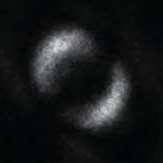
\includegraphics[scale=1]{../Images/entanglement.jpeg}}{Science Advances, Vol. 5, no.7 (2019)}
	\caption{The first ever image of quantum entanglement, where two groups of particles are sharing the physical state $\Psi(\bs{x})$, was published by \citet{moreau_imaging_2019} under the title \textit{Imaging Bell-type nonlocal behavior} in July 2019.}
	\label{fig:entanglement}
\end{figure}

The quantum theory is a fundamental theory that describes nature at the smallest scales, typically used to explain the behavior of atoms and subatomic particles. Although the theory in principle holds for systems consisting of a large number of particles as well, the calculations become both comprehensive and expensive as the system size increases, and exact computations are therefore reserved small systems. For larger systems, we in practice need to rely on approximative estimates of the observable, which also fast becomes infeasible when the system size increase.

In the most general form, the theory is based on the time-dependent Schrödinger equation,
\begin{empheq}[box={\mybluebox[5pt]}]{equation}
i\hbar\frac{\partial}{\partial t}\ket{\Psi(\bs{x},t)}=\hat{\mathcal{H}}\ket{\Psi(\bs{x},t)}
\end{empheq}
which describes the state, or the wave function, $\Psi(\bs{x},t)$, of a system with Hamilton operator $\hat{\mathcal{H}}$, known as the Hamiltonian. $\bs{x}=(\bs{r},\sigma)$ specifies the coordinates and the spin of a particle, $\hbar$ is the reduced Planck's constant and $i$ is the solution of the equation $x^2=-1$. As we later will see, the quantum mechanical system is completely specified by the wave function, so by solving the equation we will in principle know anything about the system. 

\citet{schrodinger_undulatory_1926} introduced the now-called Schrödinger equation in a 1926 paper as one of many contributions to the quantum mechanics at that time. Other contributors include \citet{born_zur_1926} who suggested now-standard interpretation of the probability density function as $|\Psi(\bs{x},t)|^2$ in 1926 and his companion \citet{heisenberg_uber_1925}, who formulated the matrix mechanics representation in 1925. However, many physicists were skeptical about the new theory, including Albert Einstein and Schrödinger himself. The theory differed from the classical mechanics in the sense that it was based on a statistical interpretation, with some strange consequences. For instance, the theory allowed negative kinetic energies to occur with the consequence that a particle could \textit{go through} a potential wall, known as quantum tunneling. Later, Einstein \cite{einstein_can_1935} also pointed out that when pairs or groups of particles are generated in ways such that the wave function of each particle cannot be described independently of the other state, they will be affected by each other even at large distances. He called this \textit{"spooky action at a distance"}, and used the observation to argument that the quantum theory had to be incorrect. However, the observation was later proven to be correct and as late as in July 2019 the first image of quantum entanglement, as the phenomenon is called, was captured by \citet{moreau_imaging_2019}. See figure \eqref{fig:entanglement}.

Today, there is wide agreement in the physics society on the quantum theory. Actually, the theory is the most precisely tested in the history of science, where computed observable of atoms agree perfectly with experiments. Most notably, quantum electrodynamical calculations of the fine structure constant $\alpha$ are, by \citet{odom_new_2006}, found to agree with experiments within ten parts in a billion, $10^{-8}$.\bigskip

In this chapter, we will first state the postulates of quantum mechanics, and thereafter we discuss the time-independent Schrödinger equation and challenges related to solving it. As we will see, every observable in quantum mechanics is associated with an operator. The consequence is that all obtained values are identified with standard errors which are also important to specify in order to present the accuracy of the value. In that manner, quantum mechanics is based on statistics, and in section \ref{sec:statisticalinterpretation} we discuss the statistical interpretation of the theory. The variational principle states that the ground state energy is the lowest possible energy calculated, so by minimizing the energy in a variational scheme, a ground state energy estimation can be obtained. Other things discussed are the quantum numbers, which are the values that give acceptable solutions to the Schrödinger equation, and the virial theorem, which relates kinetic and potential energy. 

Albeit the quantum mechanics will make up the framework for this work, we will in this chapter only discuss the theory needed for the work, and this is therefore not meant as an encyclopedia to quantum mechanics. For a complete introduction to the topic, \textit{Introduction to Quantum Mechanics} written by \citet{griffiths_introduction_2005} serves as an excellent read. Before we get started, we make a few assumptions in order to simplify our problem. The most important ones are specified below with an explanation of why they are valid.

\begin{itemize}
	\item \textbf{Point-like particles:} First, all particles involved will be assumed to be point-like, i.e., they lack spatial extension. For electrons, this makes sense since they, as far as we know, do not extend. The assumption is also applied to the nucleus in atomic systems, but it still makes sense since the distance from the nucleus to the electrons is known to be much larger than the nucleus extension.
	
	\item \textbf{Non-relativistic spacetime:}  Second, we operate in the non-relativistic spacetime, which is an excellent approximation as long as we do not approach the speed of light and we do not involve strong forces. Applying classical physics, we can find that the speed of the electron in a hydrogen atom is about 1\% of the speed of light. Even though the electrons achieve higher velocities in heavy atoms, we do not need to worry about it as we will stick to the lighter atoms. In the quantum dots, this assumption holds even for large systems, as the velocity and density will still be sufficiently low.
	
	\item For specific systems, we might make new assumptions and approximations. For instance, for atomic systems, we will assume that the nucleus is at rest. Those approximations will be discussed consecutively. 
\end{itemize}

\section{The postulates of quantum mechanics} \label{sec:postulates}
Quantum mechanics is characterized by a set of fundamental axioms that make up the base of the theory. As we assume that they always hold, every statement in quantum mechanics is based on them, and it is, therefore, natural to list them now in the beginning. They can be formulated by six postulates, in the following way:

\begin{enumerate}
	\item \textit{"The state of a quantum mechanical system is completely specified by the wave function $\Psi(\bs{x},t)$."}
	
	\item \textit{"To every observable in classical mechanics, there corresponds a linear, Hermitian operator in quantum mechanics."}
	
	\item \textit{"In any measurement of the observable associated with an operator $\hat{O}$, the only values that will ever be observed are the eigenvalues $o$ which satisfy $\hat{O}\Psi(\bs{x},t)=o\Psi(\bs{x},t)$."}
	
	\item \textit{"The expectation value of the observable corresponding to operator $\hat{O}$ is given by
		$$\langle\hat{O}\rangle=\frac{\int d\tau\Psi^*(\bs{x},t)\hat{O}\Psi(\bs{x},t)}{\int d\tau\Psi^*(\bs{x},t)\Psi(\bs{x},t)}.\textit{"}$$}
	
	\item \textit{"The wave function evolves in time according to the time-dependent Schrödinger equation,
		$$\hat{\mathcal{H}}\Psi(\bs{x},t)=i\hbar\frac{\partial\Psi(\bs{x},t)}{\partial t}.\textit{"}$$}
	
	\item \textit{"The total wave function must be anti-symmetric concerning the interchange of all coordinates of one fermion with those of another. Electronic spin must be included in this set of coordinates."} 
\end{enumerate}
All the postulates will be used in this work, and they will be described in detail when we need them. Albeit we will look at stationary states only, even the time-dependent Schrödinger from the fifth postulate will be discussed due to the description of the diffusion Monte Carlo method in section \ref{sec:dmc}. The other will be covered in the current and the next chapter. The formulation of the presented postulates are taken from \cite{sherrill_david_postulates_2003}.

\section{The Schrödinger equation} \label{sec:schrodinger}
We have already presented the time-dependent Schrödinger equation on several occasions, but as mentioned above, we will in this work study stationary systems only. If we also recall that the particles are assumed to be non-relativistic, the focus will be on solving the time-independent non-relativistic Schrödinger equation. By defining $\Psi_n(\bs{x})$ as the wave function of a state $n$ with energy $\varepsilon_n$, the equation can be expressed as
\begin{empheq}[box={\mybluebox[5pt]}]{equation}
\label{eq:Energy}
\hat{\mathcal{H}}\psin=E_n\psin
\end{empheq}
where $\hat{\mathcal{H}}$ is the aforementioned Hamiltonian, the total energy operator. By analogy with the classical mechanics, the total mechanical energy is the kinetic and potential energy summarized,
\begin{equation}
\hat{H}=\hat{T}+\hat{V}
\end{equation}
with $\hat{T}$ and $\hat{V}$ as the kinetic and potential energy operators respectively. 

Again from classical mechanics, the kinetic energy of a moving particle of mass $m$ yields $T=p^2/2m$ where $p$ is the (linear) momentum, such that the kinetic energy operator can be represented as 
\begin{equation}
\hat{T}=\frac{\hat{p}^2}{2m},
\end{equation}
according to Ehrenfest's theorem. Further, the momentum operator is $\hat{p}=-i\hbar\hat{\nabla}$ with $\hat{\nabla}$ as the differential operator and the factor $i\hbar$ arising from the canonical commutator relation between the position operator and the momentum operator,
\begin{equation}
[\hat{x},\hat{p}]=\hat{x}\hat{p}-\hat{p}\hat{x}=i\hbar,
\end{equation}
which indicates that the momentum and the position do not \textit{commute}. In other words, the order of the operators in an equation is not arbitrary. The potential, on the other hand, is obviously dependent on the system we want to study. For atomic systems, the potential as a function of the distance from the nucleus can be found from Coulomb's law and reads 
\begin{equation}
V(r)=\frac{1}{4\pi\epsilon_0}\frac{Ze^2}{r}
\label{eq:atompotential}
\end{equation}
where the nucleus is assumed to be at rest at the origin, $k_e=1/4\pi\epsilon_0$ is the Coulomb constant, $Z$ is the atomic number of the nucleus, and $e$ is the elementary charge. For a general potential, the Hamiltonian can be expressed as 
\begin{equation}
\hat{\mathcal{H}}=-\frac{\hbar^2}{2m}\nabla^2+V(r)
\label{eq:oneparticlehamiltonian}
\end{equation}
which is the farthest we can go without specifying the external potential $V(r)$.

By setting up equation \eqref{eq:Energy} with respect to the energies, we obtain an integral,
\begin{equation}
E_n=\frac{\int d\bs{r}\psinc\hat{\mathcal{H}}\psin}{\int d\bs{r}\psinc\psin},
\label{eq:energyintegral}
\end{equation}
which not necessarily is trivial to solve. For almost\footnote{Exceptions include quantum dots of two electrons in two and three dimensions, where Taut has presented semi-analytical energies for a few oscillator frequencies \cite{taut_two_1993,taut_two_1994}.} all many-electron systems, this becomes analytically infeasible due to a two-body interaction term. This will be covered in chapter \ref{chp:manybody}.

As suggested by Max Born, we get the probability density function if we take the dot product between the complex conjugate wave function and the wave function itself,
\begin{equation}
P(\bs{r})=\psinc\psin=|\psin|^2,
\label{eq:pdf}
\end{equation}
so the denominator in equation \eqref{eq:energyintegral} is basically the integral over all the probabilities. If the wave function is normalized correctly, this should always give 1. 

As a very brief example, we will below calculate the bounding energy of the Hydrogen atom.

\subsection{The Hydrogen atom} \label{sec:hydrogen}
We presented the one-particle Hamiltonian in equation \eqref{eq:oneparticlehamiltonian}, and the potential from the nucleus in equation \eqref{eq:atompotential}. By introducing the Bohr radius
\begin{equation}
a_0=\frac{4\pi\epsilon_0\hbar^2}{m_eZe^2}
\end{equation}
we can set up the total Hamiltonian as
\begin{equation}
\hat{\mathcal{H}}\cdot\frac{(4\pi\epsilon_0)^2\hbar^2}{m_eZ^2e^4}=-\frac{1}{2}a_0^2\nabla^2-\frac{a_0}{r}
\end{equation}
where we have multiplied all the terms by the factor $(4\pi\epsilon_0)^2\hbar^2/m_eZ^2e^4$ in order to make the equation dimensionless. We can further scale the energy as $E\leftarrow E\cdot (4\pi\epsilon_0)^2\hbar^2/m_eZ^2e^4$ and the distance as $r\leftarrow r/a_0$, which both are dimensionless, and obtain the Hamiltonian
\begin{equation}
\hat{\mathcal{H}}=-\frac{1}{2}\nabla^2-\frac{1}{r}
\end{equation}
where all quantities are in atomic units.

The Hydrogen ground state wave function is well-known and reads
\begin{equation}
\Psi(r)\propto e^{-r}
\end{equation}
in atomic units. The binding energy in Hydrogen is found from the Schrödinger equation in equation \eqref{eq:Energy}, and gives
\begin{equation}
\hat{\mathcal{H}}\Psi(r)=\bigg(-\frac{1}{2}\nabla^2-\frac{1}{r}\bigg)\Psi(r)=-\frac{1}{2}\Psi(r)
\end{equation}
which indicates that $E_0=-0.5$.


\section{Statistical interpretation} \label{sec:statisticalinterpretation}
In equation \eqref{eq:energyintegral}, we found the expectation value of the energy using the Hamiltonian, which is the energy operator. By the second postulate of quantum mechanics, every observable in the classical mechanics is associated with such a Hermitian operator $\hat{O}$ related to an expectation value $\langle \hat{O}\rangle$ is the same way,
\begin{equation}
\langle \hat{O}\rangle=\frac{\int d\bs{r}\psinc\hat{O}\psin}{\int d\bs{r}\psinc\psin}.
\label{eq:generalexp}
\end{equation}
As a consequence, there is always an uncertainty associated with a quantum mechanical calculation, such that we can only tell the probability of measuring something. The uncertainty is usually described by the variance, which for a set of independent measurements is given by
\begin{equation}
\sigma^2=\langle \hat{O}^2\rangle-\langle \hat{O}\rangle^2.
\label{eq:variance}
\end{equation}
If there are correlations between the measurements, this expression underestimates the actual sampling variance as the \textit{covariance} is not taken into account, which is detailed in section \ref{sec:variance}. If we take the square root of the variance, we obtain the standard deviation, which is the quantity given as the standard error in the results. From the standard deviation, a variety of mathematical inequalities follows, where Heisenberg's uncertainty principle is the most famous. It states that the more precisely the position of some particle is determined, the less precisely its momentum can be known, and is mathematically presented as
\begin{empheq}[box={\mybluebox[5pt]}]{equation}
\sigma_x\sigma_p\geq\frac{\hbar}{2}
\end{empheq}
where $\sigma_x$ is the standard deviation of the position and $\sigma_p$ is the standard deviation of the momentum.

The general expected value in equation \eqref{eq:generalexp} is expressed using the Schrödinger wave mechanics picture, but it can also be written in terms of, for instance, the Heisenberg picture applying matrices. However, the standard formalism today in most branches of the quantum mechanics is the Dirac notation, which relates the Schrödinger picture and the Heisenberg picture elegantly. Using this, the expectation value from equation \eqref{eq:generalexp} reads
\begin{equation}
\langle \hat{O}\rangle=\frac{\mel{\Psi}{\hat{O}}{\Psi}}{\braket{\Psi}{\Psi}}
\end{equation}
where $\bra{\Psi}$ is called the \textit{bra} and $\ket{\Psi}$ is called the \textit{ket}. For that reason, the formalism is also called bracket formalism. Usually, the wave function is assumed to be normalized, which further simplifies the expected value to
\begin{equation}
\langle \hat{O}\rangle=\mel{\Psi}{\hat{O}}{\Psi},
\end{equation}
and will henceforth be assumed. More information about the Dirac formalism can be found in Appendix \ref{app:dirac}. 

\section{The variational principle} \label{sec:variationalprinciple}
In the equations above, the presented wave functions are assumed to be the exact eigenfunctions of the Hamiltonian. However, often we do not know the exact wave functions, and we need to guess what the wave functions might be. In those cases, we apply the variational principle, which states that only the exact ground-state wave function can give the ground state energy. All other wave functions that fulfill the required properties (see section \ref{sec:wavefunction}) give higher energies, and mathematically we can express the statement as
\begin{empheq}[box={\mybluebox[5pt]}]{equation}
E_0\leq\mel{\Psi}{\hat{\mathcal{H}}}{\Psi}
\label{eq:variationalprinciple}
\end{empheq}
where $\Psi$ is an arbitrary wave function. The variational method is a way of finding approximations to the energy ground state, which is based on the variational principle. Most notably, the variational Monte Carlo method is named after the principle and attempts to solve the integrals directly by varying a trial wave function. The variational principle ensures that the obtained energy never goes below the ground state energy, as further described in chapter \ref{chp:methods}. Other methods that apply the variational method are the famous Hartree-Fock method and the infamous coupled cluster method.

\section{Quantum numbers}
Unlike in classical mechanics, all the observable in quantum mechanics are discrete or \textit{quantized}, which means that the $n$ associated with $E_n$ above cannot take any number. $n$ can only take positive integers and is named the principal quantum number. We also have other quantum numbers identified with the angular momentum and spin as described below.

\subsection*{Principal}
The \textbf{principal} quantum number describes the electron shell, and can take the numbers $n\in[1,2,3,\hdots)$. As $n$ increases, the electron excites to a higher shell such that also the energy increases. In general, $E_1<E_2<E_3\hdots$ as long as all other quantum numbers are fixed. The electron shells can again be split up in subshells, requiring more quantum numbers.

\subsection*{Angular}
An electron shell can possibly have more than one subshell, described by the \textbf{angular} quantum number $l$. $l$ can take the values $0,1,\hdots n-1$, such that the degeneracy of subshells in a shell is simply $n$. In atoms, the angular quantum number describes the shape of the shell, where $l=0$ gives a spherical shape, $l=1$ gives a polar shape while $l=2$ gives a cloverleaf shape. 

\subsection*{Magnetic}
We also have a \textbf{magnetic} quantum number $m_l$, which has the range $-l,-l+1,\hdots,l-1,l$. If $l$ describes the shape of a shell, $m_l$ specifies its orientation in space. This quantum number was first observed under the presence of a magnetic field, hence the name.

\subsection*{Spin}
The \textbf{spin} quantum number $s$ gives the spin of a particle, which can just be seen as a particle's property. Particles are often divided into two groups depending on the spin because of their different behavior: \textbf{bosons} have integer spin, while \textbf{fermions} have half-integer spin. Electrons and protons have spin $s=1/2$, which makes them fermions.

\subsection*{Spin projection}
The last number we will discuss is the \textbf{spin projection} quantum number $m_s$. It has the range $-s,-s+1,\hdots,s-1,s$, and is therefore related to the spin quantum number in the same way as the magnetic number $m_l$ is related to the angular number $l$. Electrons can for that reason take the values $m_s=+1/2$ or $m_s=-1/2$, such that there are two groups of electrons. The consequences will be discussed in the section \ref{sec:wavefunction}.

\section{The virial theorem} \label{sec:virial}
The virial theorem relates the kinetic energy to the potential energy, and makes it possible to find the (time) average of the kinetic energy even for complex systems. The classical statement of the theorem was formulated during the 19th century and named by \citet{clausius_xvi._1870} in 1870. It is in the most general form given by 
\begin{empheq}[box={\mybluebox[5pt]}]{equation}
\langle\hat{T}\rangle=-\frac{1}{2}\sum_{i=1}^N\langle\bs{F}_i\cdot\bs{r}_i\rangle_t,
\label{eq:virialtheorem}
\end{empheq}
where $\bs{F}_i$ represents the force on particle $i$ at position $\bs{r}_i$. The quantum mechanical version was proven by \citet{fock_bemerkung_1930} in a 1930 paper, where the expectation value of the force is represented with $d\langle p\rangle/dt$. For potential sources in the form of $V_i=ar^{n_i}$, we can use Ehrenfest's theorem to express the virial theorem in a simpler fashion,
\begin{equation}
2\langle \hat{T} \rangle = \sum_{i}n_i\langle \hat{V}_{i} \rangle.
\label{eq:simplevirial}
\end{equation}
The same expression can be found in classical physics as well, using the relation $\bs{F}=-\nabla V$. The virial theorem requires that the system is in a bound state. An example on a system that does not fulfill the requirements, is a comet that has enough kinetic energy to escape a planet's gravitational field. 

On the other hand, the Hydrogen atom, discussed in section \ref{sec:hydrogen}, satisfies the virial theorem as the potential is in the form of $V(r)\propto r^{-1}$ and the electron is bounded. For that particular case, the virial theorem reads $2\langle\hat{T}\rangle=-\langle\hat{V}\rangle$, which means that $\langle\hat{H}\rangle=\langle\hat{V}\rangle/2$. However, if we add another electron and get a Hydrogen anion, the simplified virial theorem in equation \eqref{eq:simplevirial} breaks down because of the interaction.

It is also important to emphasize that the expectation value discussed above is, in principle, the time average of the operator. However, if the ergodic hypothesis holds for the system, i.e., the ensemble average is equal to the time average, an ensemble average can also be taken \cite{flyvbjerg_error_1989}.

\iffalse
\subsubsection*{Angular Momentum and Spin}
Relation between the angular and spin quantum number

(One last analogy with the classical mechanics)

If we again go back to the classical mechanics, the angular momentum $\bs{L}_r=\bs{R}\cross\bs{p}$ around an axis at distance $|\bs{R}|$ from the mass center and the angular momentum $\bs{L}_c=I\bs{\omega}$ around its own mass center is a conserved quantity,
\begin{equation}
\bs{L}_{net} = \bs{L}_r+\bs{L}_c.
\end{equation}
Since the net angular momentum $\bs{L}_{new}$ is just a sum over the angular momentum of all points in a continua around the rotational axis given by the definition of $\bs{L}_r$, both of them are actually the same thing.

In quantum mechanics we have again an analogy, where we define a \textbf{spin} $s$ which describes a particles rotation around its own mass center and a \textbf{angular momentum} $l$ which describes a particles rotation around an external rotational axis. Like in classical physics, the total spin $S$ and the total angular momentum $L$ is a conserved quantity,
\begin{equation}
J=L+S,
\end{equation}
but the transition from $L$ to $S$ is rare compared to the transition from $L_c$ to $L_r$. Spin-orbit coupling. Azimuthal. Quantized.
\fi
    \chapter{Many-body Quantum Mechanics} \label{chp:manybody}
\epigraph{We have to remember that what we observe is not nature in itself but
	nature exposed to our method of questioning.}{Werner Heisenberg, \supercite{heisenberg_across_1990}}
\begin{figure}[H]
	\centering
	\captionsetup[subfigure]{labelformat=empty}
	\copyrightbox[l]{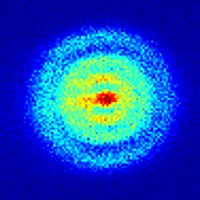
\includegraphics[scale=3]{../Images/art_quantum.jpg}}{Physical review letters,\\ 110, 213001 (2013)}
	\caption{The first photograph of a hydrogen atom was captured by an ultra sensitive camera in 2013. One can actually see the probability distribution $|\Psi(\bs{x})|^2$ with the naked eye. Published by \citet{stodolna_hydrogen_2013} with the title \textit{Hydrogen atoms under magnification}.}
\end{figure}

\sloppy
In the previous chapter, the quantum mechanics of single particles was discussed. We presented the time-independent Schrödinger equation, and from that, we obtained a general expression of the energy of a stationary particle. The energy expression of a stationary many-particle system is almost identical,
\begin{equation}
E_n=\mel{\Psi_n(\bs{X})}{\hat{\mathcal{H}}}{\Psi_n(\bs{X})},
\label{eq:energy}
\end{equation}
but we here use the many-body wave function $\Psi_n(\bs{X})$ of state $n$ with $\bs{X}=\{\bs{x}_1,\bs{x}_2,\cdots,\bs{x}_N\}=\{\{\bs{r}_1, \sigma_1\}, \{\bs{r}_2, \sigma_2\},\cdots,\{\bs{r}_N, \sigma_N\}\}$ denoting the collective coordinates and the spins of all the $N$ particles in the system. The Hamiltonian, $\hat{\mathcal{H}}$, defines the system and is given explicitly in the next section. As noted before, the wave function of large systems needs to store an immense amount of information and is therefore impractical or even impossible to deal with. In this section, we will first look at how the many-body Hamiltonian is composed, before we have an extensive discussion of how the many-body wave function is constructed.

\section{The electronic Hamiltonian} \label{sec:electronichamiltonian}
We have already seen what the one-body Hamiltonian looks like, and the many-body Hamiltonian is not very different. We recall that it can be split in a kinetic and a potential term,
\begin{equation}
\hat{H}=\hat{T}+\hat{V}
\end{equation}
where $\hat{T}$ is the kinetic energy and $\hat{V}$ is the potential energy. Nevertheless, as we study electrons, they are charged and will therefore interact with each other. For that reason, we need to add an interaction term to the Hamiltonian, which in general is included in the potential term $V=V_{\text{ext}}+V_{\text{int}}$ with $V_{\text{ext}}$ as the external potential and $V_{\text{int}}$ as the interaction potential. In the same way as the nucleus potential, the interaction potential is given by Coulomb's law, for two electrons given by 
\begin{equation}
V_{\text{int}} =k_e\frac{e^2}{r_{12}}
\end{equation}
where $r_{12}$ is the distance between the electrons. For a general system containing $N$ electrons, the total Hamiltonian can therefore be expressed as 
\begin{empheq}[box={\mybluebox[5pt]}]{equation}
\hat{\mathcal{H}}=-\sum_{i=1}^N\frac{\hbar^2}{2m_e}\nabla_i^2+\sum_{i=1}^{N}V_i + \sum_{i=1}^N\sum_{j>i}^Nk_e\frac{e^2}{r_{ij}}
\label{eq:ElectronicHamiltonian}
\end{empheq}
without specifying the external potential, $V_i$. The relative distance between particle $i$ and $j$ is defined by $r_{ij}\equiv|\bs{r}_i-\bs{r}_j|$. From now on, we will use atomic units setting $\hbar=m_e=k_e=e=1$, see appendix \ref{app:units} for details.

By putting the Hamiltonian in equation \eqref{eq:ElectronicHamiltonian} into equation \eqref{eq:energy}, the integral can be split in three terms,
\begin{equation}
\begin{aligned}
E_n&=\sum_{i=1}^N\bigg[-\frac{1}{2}\mel{\Psi_n(\bs{X})}{\nabla_i^2}{\Psi_n(\bs{X})}
+\mel{\Psi_n(\bs{X})}{V_i}{\Psi_n(\bs{X})}
+\sum_{j>i}^N\mel{\Psi_n(\bs{X})}{\frac{1}{r_{ij}}}{\Psi_n(\bs{X})}\bigg]
\end{aligned}
\end{equation}
where the two former ones are the one-body integrals, or \textit{matrix elements}, which in many cases can be solved analytically. However, the last term is often difficult to solve, and in fact there are analytical solutions available for the two-particle case only. In other words, a precise evaluation of this integral can usually only be found using numerical methods, which we will have a closer look at in chapter \ref{chp:methods} in conjunction with quantum Monte Carlo methods.

\section{The many-body wave function} \label{sec:wavefunction}
By the first postulate of quantum mechanics presented in section \ref{sec:postulates}, the wave function contains all the information specifying the state of the system. This means that all observable in classical mechanics can in principle also be estimated from the wave function, which makes finding the wave function our aim. As discussed in chapter \ref{chp:quantum}, we can define the wave function for a single particle, known as the \textit{single-particle function} (SPF), $\psi(\bs{r},\sigma)$. Can we combine the SPFs of the electrons in a system and obtain the many-body wave function? Possibly, the most straight-forward way of doing this is to simply multiply all the SPFs,
\begin{equation}
\Psi(\bs{X})=\psi(\bs{r}_1,\sigma_1)\psi(\bs{r}_2,\sigma_2)\cdots\psi(\bs{r}_N,\sigma_N),
\end{equation}
known as the \textit{Hartree product}. However, this product is generally not correct, as it does not include the required symmetry properties of the many-body wave function. Instead, we can take the symmetry into account by expressing the many-body wave function as a determinant or a permanent, as we will see in section \ref{sec:slater}. Together with the symmetry properties, there is an array of requirements the wave function needs to meet in order to be physically correct. Some of them are:

\iffalse
We will in this section discuss the symmetry properties of the wave function for bosonic and fermionic systems, and see how the wave function can be set up as a Slater determinant in order to meet these properties. Also, Jastrow factors will be touched, as they are used in quantum Monte Carlo methods to handle the correlations. With that in mind, we approximate the \textit{trial} wave function by a Slater-Jastrow function,
\begin{equation}
\Psi_T(\bs{r};\bs{\theta})=|\hat{D}(\bs{r};\bs{\theta})|J(\bs{r};\bs{\theta}),
\end{equation}
which is an educated guess of the form of the wave function. 
Here the first part, $|\hat{D}(\bs{r};\bs{\theta})|$, is the Slater determinant and $J(\bs{r};\bs{\theta})$ is a Jastrow factor with $\theta$ as some variational parameters. Other quantum many-body methods, such as full configuration interaction and coupled cluster use a linear expansion of Slater determinants to approximate the wave function, while the Hartree-Fock method relies on one single Slater determinant (without any Jastrow factor). Nevertheless, as we will focus on quantum Monte Carlo methods, this chapter will be tailored to the method. 

The trial wave function needs to satisfy some requirements in order to be used in the variational principle, and we thus need to make an educated guess on the wave function where the requirements are fulfilled. The requirements are the following:
\fi

\begin{enumerate}
	\item \textbf{Normalizability:} The wave function needs to be normalizable in order to make physical sense. The total probability should always be 1, and a wave function that cannot be normalized will not have a finite total probability. The consequence is that the wave function goes to zero when the positions get large, $\Psi(x\rightarrow\pm\infty)\rightarrow 0$. 
	
	\item \textbf{Cusp condition:} The cusp condition, or the Kato theorem, states that the wave function should have a cusp where the potential explodes. An example on this is when electrons come close to each other, i.e., the electron-electron cusp.
	
	\item \textbf{Symmetry and anti-symmetry:} The wave function needs to be either symmetric or anti-symmetric under the exchange of two coordinates, dependent on whether the electrons are fermions or bosons. This is the statement of the sixth postulate, which will be further explained in the next section.
\end{enumerate}

\subsection{Anti-symmetry and the Pauli principle} \label{sec:symmetry}
Symmetry and anti-symmetry are central concepts in quantum mechanics, and often one can use symmetry arguments to simplify expressions and calculations. Assume that we have a permutation operator, $\hat{P}(i\rightarrow j)$, which exchanges the coordinates of the particles $i$ and $j$ in the many-body wave function containing $M$ particles,
\begin{equation}
\hat{P}(i\rightarrow j)\Psi_n(\bs{x}_1,\cdots,\bs{x}_i,\cdots,\bs{x}_j,\cdots,\bs{x}_M)=p\Psi_n(\bs{x}_1,\cdots,\bs{x}_j,\cdots,\bs{x}_i,\cdots,\bs{x}_M),
\end{equation}
where $p$ is the eigenvalue coming from the transformation. If we again apply the $\hat{P}$ operator, we should switch the same coordinates back, and we expect to end up with the initial wave function. For that reason, $p$ must be either +1 or -1. \footnote{Actually, in two-dimensional systems a third possibility is allowed which gives an \textit{anyon}. The theory on this was developed by \citet{leinaas_one_1977} during the 1970s.} The particles that have an anti-symmetric wave function under the exchange of two coordinates are called fermions, named after Enrico Fermi, and as discussed before, they have half-integer spin. On the other hand, the particles that have a symmetric wave function under the exchange of two coordinates are called bosons, named after Satyendra Nath Bose, and have integer spin. A consequence of the anti-symmetric wave function is that two identical fermions cannot occupy the same state at the same time, known as the Pauli principle. This means that identical fermions even in the many-particle ground state (at zero temperature) spread over multiple states, and in the next section, we will see how this principle is included in the wave function through a Slater determinant. 

\subsection{The Slater determinant} \label{sec:slater}
For a system of many particles, we can define a many-body wave function, which is a composition of all the SPFs and contains all the information about the system as the first postulate, discussed in section \ref{sec:postulates}, requires. For fermions, we need to combine the SPFs such that the Pauli principle is fulfilled at all times, which can be accomplished by a determinant. 

Consider a system of two identical fermions with SPFs $\psi_1(\bs{r},\sigma)$ and $\psi_2(\bs{r},\sigma)$ with coordinates and spin $\boldsymbol{r}_1,\sigma_1$ and $\boldsymbol{r}_2,\sigma_2$ respectively. The way we define the wave function of the system is then
\begin{equation}
\begin{aligned}
\Psi(\bs{X})&=\frac{1}{\sqrt{2}}
\begin{vmatrix}
\psi_1(\boldsymbol{r}_1,\sigma_1) & \psi_2(\boldsymbol{r}_1,\sigma_1)\\
\psi_1(\boldsymbol{r}_2,\sigma_2) & \psi_2(\boldsymbol{r}_2,\sigma_2)
\end{vmatrix}\\
&=\frac{1}{\sqrt{2}}\Big[\psi_1(\boldsymbol{r}_1,\sigma_1)\psi_2(\boldsymbol{r}_2,\sigma_2)-\psi_2(\boldsymbol{r}_1,\sigma_1)\psi_1(\boldsymbol{r}_2,\sigma_2)\Big],
\end{aligned}
\end{equation}
which is equates to zero if the particles happen to be at the same position and have the same spin at the same time. If the particles, on the other hand, have different spins, they are allowed to appear at the same spatial state at the same time and the determinant will not equate to zero. For larger systems, the Slater determinant is constructed in the same way as above, and any pair of identical particles located in the same state will make the determinant collapse. A Slater determinant containing $N$ electrons reads
\begin{equation}
\Psi(\bs{X})=\frac{1}{\sqrt{N!}}
\begin{vmatrix}
\psi_1(\boldsymbol{r}_1,\sigma_1) & \psi_2(\boldsymbol{r}_1,\sigma_1) & \cdots & \psi_N(\boldsymbol{r}_1,\sigma_1)\\
\psi_1(\boldsymbol{r}_2,\sigma_2) & \psi_2(\boldsymbol{r}_2,\sigma_2) & \cdots & \psi_N(\boldsymbol{r}_2,\sigma_2)\\
\vdots & \vdots & \ddots & \vdots \\
\psi_1(\boldsymbol{r}_N,\sigma_N) & \psi_2(\boldsymbol{r}_N,\sigma_N) & \cdots & \psi_N(\boldsymbol{r}_N,\sigma_N)
\end{vmatrix}
\end{equation}
where the $\psi(\bs{r},\sigma)$ is the tensor product between the radial part $\phi(\bs{r})$ and the spin part $\xi(\sigma)$,
\begin{equation}
\psi(\bs{r},\sigma)=\phi(\bs{r})\otimes\xi(\sigma).
\end{equation}
In section \ref{sec:slaterdeterminant}, it is shown that the Slater determinant can be split in a spin-up part and a spin-down part such that the spin-dependency $\xi(\sigma)$ can be omitted. For that reason, we can define a basis set consisting of the spatial parts only, discussed in the next section. 

As a note, we will in the rest of this thesis use $\Psi$ as the many-particle wave function, $\psi$ are the SPFs, and $\phi$ is the spatial part of the SPF. We reserve $\xi$ for the spin part of the SPFs, but it will often be omitted as the spin-part can be factorized out. Sometimes it is appropriate to split up the many-particle wave function, and we will, in that case, denote each part by $\Psi_i$ where $i$ is an index associated with the particular element. Lastly, the basis functions will be denoted by $\varphi$, which we will discuss in the next section.

\subsection{Basis set} \label{sec:basisset}
In quantum chemistry, a basis set usually refers to a set of one-particle functions used to build the SPFs discussed above. The basis functions depict the eigenstates of atoms, and are therefore often called \textit{atomic orbitals}. On the other hand, the SPFs are linear combinations of the atomic orbitals suited for describing the the wave-like behavior of an electron in a molecule, hence named \textit{molecular orbitals}. Commonly used atomic orbitals are Pople basis sets \supercite{ditchfield_self-consistent_1971} (in the form of x-yz G), correlation-consistent basis sets \supercite{dunning_gaussian_1989} (in the form of cc-pVNZ) and Slater-type orbitals \supercite{slater_atomic_1930} (in the form of STO-nG), where all are built on Gaussian functions. Gaussian functions are preferred as they allow efficient implementations of post Hartree-Fock methods, defined as the methods developed to improve on the Hartree-Fock method.

In our work, however, the molecular orbitals correspond to the basis functions, as we in most of the cases do not expand our SPFs, $\psi(\bs{r},\sigma)$, in a basis set. Our SPFs are typically the solution of the non-interacting system, and as the Jastrow factor is supposed to deal with the interaction, we use the same functions for the interacting case as well.

A common notation is to use the Greek letter $\varphi$ for the atomic orbitals and $\psi$ for the molecular orbitals, such that single-particle functions can be obtained from an expansion of the $N$ basis functions $\{\varphi_1(\bs{r}),\varphi_2(\bs{r}),\cdots\varphi_N(\bs{r})\}$ in the manner of
\begin{equation}
\psi_i(\bs{r})=\sum_{j=1}^Nc_{ji}\varphi_j(\bs{r}),
\label{eq:expansion}
\end{equation}
where $c_{ij}$ are the coefficients to be found. There are different approaches to obtain these coefficients, where the popular Hartree-Fock algorithm generates $c_{ij}$'s in order to find the optimal Slater determinant. For a larger basis, the results will be more accurate, but at an increasing computational cost \supercite{daniel_crawford_introduction_2007}. The actual functions used in this work are presented in chapter \ref{chp:systems} and they are linked to their respective systems. 

\subsection{Modeling the cusp} \label{sec:cusp}
From electrostatics, we know that identical, charged particles will repulse each other. This means that the probability of finding two particles close to each other should be low, which needs to be included in the wave function. To estimate observables accurately, it is crucial to model the electron-electron cusp correctly.

Different methods address this challenge in different ways. The Hartree-Fock method attempts to construct an optimal single Slater determinant by expanding the molecular orbitals in atomic orbitals, like shown in equation \eqref{eq:expansion}. The coefficients are determined such that the energy is minimized, which is performed by the Hartree-Fock algorithm \supercite{hartree_wave_1928, fock_selfconsistent_1930}. Then, we only need to deal with a Slater determinant, and as the correlations are not given explicitly, the Hartree-Fock theory is often called a mean-field theory. Further, we have post Hartree-Fock methods, like configuration interaction and the coupled cluster method, which utilize the Hartree-Fock basis, but express the wave function as a linear combination of Slater determinants, where the correlations are determined by the coefficients \supercite{daniel_crawford_introduction_2007}. If a sufficient number of Slater determinants are included in the linear combination, both the methods are capable of providing exact results. However, since the scaling goes as $N!$ and $N^6$ respectively, this is possible only for very small systems.

The variational Monte Carlo (VMC) method, which we have implemented in this work, models the electron-electron cusp in a totally different way. We there define a \textit{trial wave function}, which consists of one or more Slater determinants and a Jastrow factor, where the latter is assumed to account for the correlations. In that way, the Slater determinants are used only to account for the Pauli principle. The Jastrow factor will be discussed further in section \ref{sec:jastrow}.

Our primary focus in this work is to see if we can use machine learning to reduce the need of physical intuition. Our hope is that the method will be able to model the cusp correctly without prior knowledge about the correlations. Initially, we will try to construct a flexible Slater determinant based on neural network, which also models the correlations.

\section{Electron density} \label{sec:electrondensity}
In quantum many-body computations, the electron density is frequently calculated, and there are several reasons for that. First, the electron density can be found experimentally, such that the calculations can be benchmarked. Second, the electron density is very informative, since information about all particles can be gathered in one plot. The $P$-body electron density is defined by the multi-dimensional integral over the probability density function of all the particles but $P$, for a normalized wave function represented by
\begin{empheq}[box={\mybluebox[5pt]}]{equation}
\label{eq:electron_density}
\rho_P(\bs{r}_1,\cdots,\bs{r}_P)=N\int_{-\infty}^{\infty}d\bs{r}_{P+1}\cdots d\bs{r}_N |\Psi(\bs{r}_1,\cdots \bs{r}_N)|^2
\end{empheq}
where $P\leq N$. This integral is in general difficult to solve, and it can be found analytically for just a few realistic systems. For other systems, we need to solve the integral numerically, and we will in chapter \ref{chp:methods} describe how this can be done using Monte Carlo integration. The density should not be normalized to unit both when it is calculated analytically and numerically, but to the number of particles, i.e.,
\begin{equation}
\int_{-\infty}^{\infty}d\bs{r}_{1}\cdots d\bs{r}_P\Big[\rho_P(\bs{r}_1,\cdots,\bs{r}_P)\Big]=N.
\end{equation}

As we cannot pinpoint a particle in quantum mechanics, i.e., it is impossible to distinguish two identical particles in any way, the electron density is the same no matter which particles we decide to leave out. The standard notation is to leave out the first $P$ particles, but we could also, for instance, have left out the $P$ last particles and so forth.

So, what does the electron density tell us? The one-body density, $\rho_1(\bs{r}_1)$, is sometimes simply referred to as the electron density. It gives the probability density of finding an electron throughout the space, and give insight about how the particles are distributed in the system. On the other hand, the two-body density. $\rho_2(\bs{r}_1,\bs{r}_2)$, becomes a two-dimensional function and is therefore often expressed as a matrix. It gives the probability density of finding an electron throughout the space, given the coordinates of another particle. It, therefore, contains information about how the particles distribute relative to each other and is essential when we want to study the pairwise interaction. In systems with strong forces, such as nuclear systems, the three-body interactions become important and then it also makes sense to look at the three-body density $\rho_3(\bs{r}_1, \bs{r}_2, \bs{r}_3)$. For closed-shell circular quantum dots the radial electron density profile is often preferred as the density then also is circular and independent of the angle. 

For non-interacting systems, the wave function is separable with respect to the different particles. In those cases one can easily find the electron density analytically, since the functions of coordinates which we do not integrate over can be factorized out of the integral,
\begin{equation}
\begin{aligned}
\rho_P(\bs{r}_1,\cdots,\bs{r}_P)&=\int_{-\infty}^{\infty}d\bs{r}_{P+1}\cdots d\bs{r}_N |\Psi(\bs{r}_1),\cdots \Psi(\bs{r}_N)|^2\\
&=\int_{-\infty}^{\infty}d\bs{r}_{P+1}\cdots d\bs{r}_N |\Psi(\bs{r}_1)|^2\cdots |\Psi(\bs{r}_N)|^2\\
&=|\Psi(\bs{r}_1)|^2\cdots |\Psi(\bs{r}_P)|^2\underbrace{\int_{-\infty}^{\infty}d\bs{r}_{P+1}|\Psi(\bs{r}_{P+1})|^2\cdots\int_{-\infty}^{\infty}d\bs{r}_{N}|\Psi(\bs{r}_{N})|^2}_{=1}\\
&=|\Psi(\bs{r}_1)|^2\cdots |\Psi(\bs{r}_P)|^2,
\end{aligned}
\end{equation}
where we have assumed that the wave functions are normalized. This result has no scientific importance, but will be used to validate the implementation of the electron density in the code, see section \ref{sec:norepulsive}.

\subsection{Wigner crystals} \label{sec:wigner}
A Wigner crystal is a solid phase where electrons maximize the distance to each other in order to minimize the potential energy. As Coulomb's law gives the interaction potential, the potential is minimized when the distances between the electrons are maximized. In one-dimensional systems, the electrons are thus found at discrete locations, such that they form an evenly spaced lattice. In two-dimensional systems, the Wigner crystals form triangular lattices which are known to be the configuration that maximizes the distance in a limited space, and in three-dimensional systems, the electrons form so-called body-centered cubics. The phenomenon occurs only when the potential energy dominates the kinetic energy since the electrons then are almost "at rest" and external forces are not strong enough to push the electrons close to each other. 

If the concept still is unclear, imagine Norwegians waiting for the metro. In the nature of the people, the Norwegians always want to maximize the distance to each other, meaning that they form triangular lattices on the metro station. In extreme cases, this is equivalent to the Wigner crystals.



    \chapter{Systems} \label{chp:systems}
\epigraph{We must be clear that when it comes to atoms, language can be used only as in poetry.}{Niels Bohr, \cite{heisenberg_physics_1971}}
\begin{figure}[H]
	\centering
	%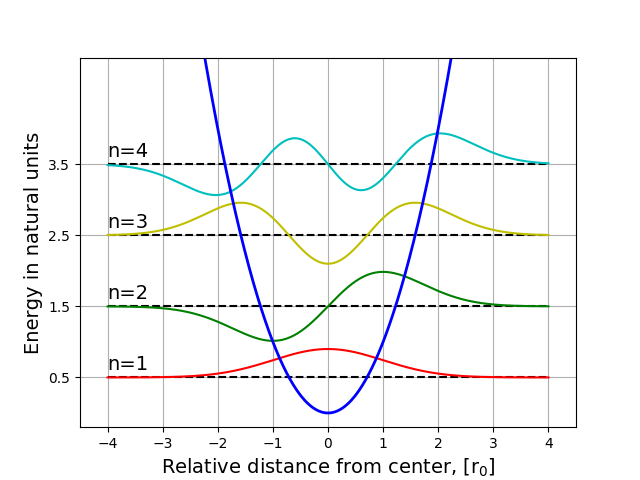
\includegraphics[scale=0.9]{Images/harmonicOscillator.png}
	% This file was created by matplotlib2tikz v0.7.4.
\begin{tikzpicture}

\begin{axis}[
%axis background/.style={fill=white!89.80392156862746!black},
axis line style={black},
tick align=outside,
tick pos=left,
tick align=outside,
tick pos=left,
x grid style={black},
xlabel={$r$},
xmajorgrids,
xmin=-4.5, xmax=4.5,
xtick={-4, -2, 0, 2, 4},
xticklabels={4, 2, 0, 2, 4},
ytick={0.5, 1.5, 2.5, 3.5},
xtick style={color=black},
y grid style={black},
ylabel={$E/\hbar\omega$},
ymajorgrids,
ymin=-0.2, ymax=5,
ytick style={color=black}
]
\addplot [semithick, black, dashed]
table {%
-4 0.5
-3.99199199199199 0.5
-3.98398398398398 0.5
-3.97597597597598 0.5
-3.96796796796797 0.5
-3.95995995995996 0.5
-3.95195195195195 0.5
-3.94394394394394 0.5
-3.93593593593594 0.5
-3.92792792792793 0.5
-3.91991991991992 0.5
-3.91191191191191 0.5
-3.9039039039039 0.5
-3.8958958958959 0.5
-3.88788788788789 0.5
-3.87987987987988 0.5
-3.87187187187187 0.5
-3.86386386386386 0.5
-3.85585585585586 0.5
-3.84784784784785 0.5
-3.83983983983984 0.5
-3.83183183183183 0.5
-3.82382382382382 0.5
-3.81581581581582 0.5
-3.80780780780781 0.5
-3.7997997997998 0.5
-3.79179179179179 0.5
-3.78378378378378 0.5
-3.77577577577578 0.5
-3.76776776776777 0.5
-3.75975975975976 0.5
-3.75175175175175 0.5
-3.74374374374374 0.5
-3.73573573573574 0.5
-3.72772772772773 0.5
-3.71971971971972 0.5
-3.71171171171171 0.5
-3.7037037037037 0.5
-3.6956956956957 0.5
-3.68768768768769 0.5
-3.67967967967968 0.5
-3.67167167167167 0.5
-3.66366366366366 0.5
-3.65565565565566 0.5
-3.64764764764765 0.5
-3.63963963963964 0.5
-3.63163163163163 0.5
-3.62362362362362 0.5
-3.61561561561562 0.5
-3.60760760760761 0.5
-3.5995995995996 0.5
-3.59159159159159 0.5
-3.58358358358358 0.5
-3.57557557557558 0.5
-3.56756756756757 0.5
-3.55955955955956 0.5
-3.55155155155155 0.5
-3.54354354354354 0.5
-3.53553553553554 0.5
-3.52752752752753 0.5
-3.51951951951952 0.5
-3.51151151151151 0.5
-3.5035035035035 0.5
-3.4954954954955 0.5
-3.48748748748749 0.5
-3.47947947947948 0.5
-3.47147147147147 0.5
-3.46346346346346 0.5
-3.45545545545546 0.5
-3.44744744744745 0.5
-3.43943943943944 0.5
-3.43143143143143 0.5
-3.42342342342342 0.5
-3.41541541541542 0.5
-3.40740740740741 0.5
-3.3993993993994 0.5
-3.39139139139139 0.5
-3.38338338338338 0.5
-3.37537537537538 0.5
-3.36736736736737 0.5
-3.35935935935936 0.5
-3.35135135135135 0.5
-3.34334334334334 0.5
-3.33533533533534 0.5
-3.32732732732733 0.5
-3.31931931931932 0.5
-3.31131131131131 0.5
-3.3033033033033 0.5
-3.2952952952953 0.5
-3.28728728728729 0.5
-3.27927927927928 0.5
-3.27127127127127 0.5
-3.26326326326326 0.5
-3.25525525525526 0.5
-3.24724724724725 0.5
-3.23923923923924 0.5
-3.23123123123123 0.5
-3.22322322322322 0.5
-3.21521521521522 0.5
-3.20720720720721 0.5
-3.1991991991992 0.5
-3.19119119119119 0.5
-3.18318318318318 0.5
-3.17517517517518 0.5
-3.16716716716717 0.5
-3.15915915915916 0.5
-3.15115115115115 0.5
-3.14314314314314 0.5
-3.13513513513514 0.5
-3.12712712712713 0.5
-3.11911911911912 0.5
-3.11111111111111 0.5
-3.1031031031031 0.5
-3.0950950950951 0.5
-3.08708708708709 0.5
-3.07907907907908 0.5
-3.07107107107107 0.5
-3.06306306306306 0.5
-3.05505505505506 0.5
-3.04704704704705 0.5
-3.03903903903904 0.5
-3.03103103103103 0.5
-3.02302302302302 0.5
-3.01501501501502 0.5
-3.00700700700701 0.5
-2.998998998999 0.5
-2.99099099099099 0.5
-2.98298298298298 0.5
-2.97497497497497 0.5
-2.96696696696697 0.5
-2.95895895895896 0.5
-2.95095095095095 0.5
-2.94294294294294 0.5
-2.93493493493493 0.5
-2.92692692692693 0.5
-2.91891891891892 0.5
-2.91091091091091 0.5
-2.9029029029029 0.5
-2.89489489489489 0.5
-2.88688688688689 0.5
-2.87887887887888 0.5
-2.87087087087087 0.5
-2.86286286286286 0.5
-2.85485485485485 0.5
-2.84684684684685 0.5
-2.83883883883884 0.5
-2.83083083083083 0.5
-2.82282282282282 0.5
-2.81481481481481 0.5
-2.80680680680681 0.5
-2.7987987987988 0.5
-2.79079079079079 0.5
-2.78278278278278 0.5
-2.77477477477477 0.5
-2.76676676676677 0.5
-2.75875875875876 0.5
-2.75075075075075 0.5
-2.74274274274274 0.5
-2.73473473473473 0.5
-2.72672672672673 0.5
-2.71871871871872 0.5
-2.71071071071071 0.5
-2.7027027027027 0.5
-2.69469469469469 0.5
-2.68668668668669 0.5
-2.67867867867868 0.5
-2.67067067067067 0.5
-2.66266266266266 0.5
-2.65465465465465 0.5
-2.64664664664665 0.5
-2.63863863863864 0.5
-2.63063063063063 0.5
-2.62262262262262 0.5
-2.61461461461461 0.5
-2.60660660660661 0.5
-2.5985985985986 0.5
-2.59059059059059 0.5
-2.58258258258258 0.5
-2.57457457457457 0.5
-2.56656656656657 0.5
-2.55855855855856 0.5
-2.55055055055055 0.5
-2.54254254254254 0.5
-2.53453453453453 0.5
-2.52652652652653 0.5
-2.51851851851852 0.5
-2.51051051051051 0.5
-2.5025025025025 0.5
-2.49449449449449 0.5
-2.48648648648649 0.5
-2.47847847847848 0.5
-2.47047047047047 0.5
-2.46246246246246 0.5
-2.45445445445445 0.5
-2.44644644644645 0.5
-2.43843843843844 0.5
-2.43043043043043 0.5
-2.42242242242242 0.5
-2.41441441441441 0.5
-2.40640640640641 0.5
-2.3983983983984 0.5
-2.39039039039039 0.5
-2.38238238238238 0.5
-2.37437437437437 0.5
-2.36636636636637 0.5
-2.35835835835836 0.5
-2.35035035035035 0.5
-2.34234234234234 0.5
-2.33433433433433 0.5
-2.32632632632633 0.5
-2.31831831831832 0.5
-2.31031031031031 0.5
-2.3023023023023 0.5
-2.29429429429429 0.5
-2.28628628628629 0.5
-2.27827827827828 0.5
-2.27027027027027 0.5
-2.26226226226226 0.5
-2.25425425425425 0.5
-2.24624624624625 0.5
-2.23823823823824 0.5
-2.23023023023023 0.5
-2.22222222222222 0.5
-2.21421421421421 0.5
-2.20620620620621 0.5
-2.1981981981982 0.5
-2.19019019019019 0.5
-2.18218218218218 0.5
-2.17417417417417 0.5
-2.16616616616617 0.5
-2.15815815815816 0.5
-2.15015015015015 0.5
-2.14214214214214 0.5
-2.13413413413413 0.5
-2.12612612612613 0.5
-2.11811811811812 0.5
-2.11011011011011 0.5
-2.1021021021021 0.5
-2.09409409409409 0.5
-2.08608608608609 0.5
-2.07807807807808 0.5
-2.07007007007007 0.5
-2.06206206206206 0.5
-2.05405405405405 0.5
-2.04604604604605 0.5
-2.03803803803804 0.5
-2.03003003003003 0.5
-2.02202202202202 0.5
-2.01401401401401 0.5
-2.00600600600601 0.5
-1.997997997998 0.5
-1.98998998998999 0.5
-1.98198198198198 0.5
-1.97397397397397 0.5
-1.96596596596597 0.5
-1.95795795795796 0.5
-1.94994994994995 0.5
-1.94194194194194 0.5
-1.93393393393393 0.5
-1.92592592592593 0.5
-1.91791791791792 0.5
-1.90990990990991 0.5
-1.9019019019019 0.5
-1.89389389389389 0.5
-1.88588588588589 0.5
-1.87787787787788 0.5
-1.86986986986987 0.5
-1.86186186186186 0.5
-1.85385385385385 0.5
-1.84584584584585 0.5
-1.83783783783784 0.5
-1.82982982982983 0.5
-1.82182182182182 0.5
-1.81381381381381 0.5
-1.80580580580581 0.5
-1.7977977977978 0.5
-1.78978978978979 0.5
-1.78178178178178 0.5
-1.77377377377377 0.5
-1.76576576576577 0.5
-1.75775775775776 0.5
-1.74974974974975 0.5
-1.74174174174174 0.5
-1.73373373373373 0.5
-1.72572572572573 0.5
-1.71771771771772 0.5
-1.70970970970971 0.5
-1.7017017017017 0.5
-1.69369369369369 0.5
-1.68568568568569 0.5
-1.67767767767768 0.5
-1.66966966966967 0.5
-1.66166166166166 0.5
-1.65365365365365 0.5
-1.64564564564565 0.5
-1.63763763763764 0.5
-1.62962962962963 0.5
-1.62162162162162 0.5
-1.61361361361361 0.5
-1.60560560560561 0.5
-1.5975975975976 0.5
-1.58958958958959 0.5
-1.58158158158158 0.5
-1.57357357357357 0.5
-1.56556556556557 0.5
-1.55755755755756 0.5
-1.54954954954955 0.5
-1.54154154154154 0.5
-1.53353353353353 0.5
-1.52552552552553 0.5
-1.51751751751752 0.5
-1.50950950950951 0.5
-1.5015015015015 0.5
-1.49349349349349 0.5
-1.48548548548549 0.5
-1.47747747747748 0.5
-1.46946946946947 0.5
-1.46146146146146 0.5
-1.45345345345345 0.5
-1.44544544544545 0.5
-1.43743743743744 0.5
-1.42942942942943 0.5
-1.42142142142142 0.5
-1.41341341341341 0.5
-1.40540540540541 0.5
-1.3973973973974 0.5
-1.38938938938939 0.5
-1.38138138138138 0.5
-1.37337337337337 0.5
-1.36536536536537 0.5
-1.35735735735736 0.5
-1.34934934934935 0.5
-1.34134134134134 0.5
-1.33333333333333 0.5
-1.32532532532533 0.5
-1.31731731731732 0.5
-1.30930930930931 0.5
-1.3013013013013 0.5
-1.29329329329329 0.5
-1.28528528528529 0.5
-1.27727727727728 0.5
-1.26926926926927 0.5
-1.26126126126126 0.5
-1.25325325325325 0.5
-1.24524524524525 0.5
-1.23723723723724 0.5
-1.22922922922923 0.5
-1.22122122122122 0.5
-1.21321321321321 0.5
-1.20520520520521 0.5
-1.1971971971972 0.5
-1.18918918918919 0.5
-1.18118118118118 0.5
-1.17317317317317 0.5
-1.16516516516517 0.5
-1.15715715715716 0.5
-1.14914914914915 0.5
-1.14114114114114 0.5
-1.13313313313313 0.5
-1.12512512512513 0.5
-1.11711711711712 0.5
-1.10910910910911 0.5
-1.1011011011011 0.5
-1.09309309309309 0.5
-1.08508508508509 0.5
-1.07707707707708 0.5
-1.06906906906907 0.5
-1.06106106106106 0.5
-1.05305305305305 0.5
-1.04504504504505 0.5
-1.03703703703704 0.5
-1.02902902902903 0.5
-1.02102102102102 0.5
-1.01301301301301 0.5
-1.00500500500501 0.5
-0.996996996996997 0.5
-0.988988988988989 0.5
-0.980980980980981 0.5
-0.972972972972973 0.5
-0.964964964964965 0.5
-0.956956956956957 0.5
-0.948948948948949 0.5
-0.940940940940941 0.5
-0.932932932932933 0.5
-0.924924924924925 0.5
-0.916916916916917 0.5
-0.908908908908909 0.5
-0.900900900900901 0.5
-0.892892892892893 0.5
-0.884884884884885 0.5
-0.876876876876877 0.5
-0.868868868868869 0.5
-0.860860860860861 0.5
-0.852852852852853 0.5
-0.844844844844845 0.5
-0.836836836836837 0.5
-0.828828828828829 0.5
-0.820820820820821 0.5
-0.812812812812813 0.5
-0.804804804804805 0.5
-0.796796796796797 0.5
-0.788788788788789 0.5
-0.780780780780781 0.5
-0.772772772772773 0.5
-0.764764764764765 0.5
-0.756756756756757 0.5
-0.748748748748749 0.5
-0.740740740740741 0.5
-0.732732732732733 0.5
-0.724724724724725 0.5
-0.716716716716717 0.5
-0.708708708708709 0.5
-0.700700700700701 0.5
-0.692692692692693 0.5
-0.684684684684685 0.5
-0.676676676676677 0.5
-0.668668668668669 0.5
-0.660660660660661 0.5
-0.652652652652653 0.5
-0.644644644644645 0.5
-0.636636636636636 0.5
-0.628628628628629 0.5
-0.620620620620621 0.5
-0.612612612612613 0.5
-0.604604604604605 0.5
-0.596596596596596 0.5
-0.588588588588589 0.5
-0.580580580580581 0.5
-0.572572572572573 0.5
-0.564564564564565 0.5
-0.556556556556556 0.5
-0.548548548548549 0.5
-0.54054054054054 0.5
-0.532532532532533 0.5
-0.524524524524525 0.5
-0.516516516516516 0.5
-0.508508508508509 0.5
-0.5005005005005 0.5
-0.492492492492492 0.5
-0.484484484484485 0.5
-0.476476476476476 0.5
-0.468468468468469 0.5
-0.46046046046046 0.5
-0.452452452452452 0.5
-0.444444444444445 0.5
-0.436436436436436 0.5
-0.428428428428429 0.5
-0.42042042042042 0.5
-0.412412412412412 0.5
-0.404404404404405 0.5
-0.396396396396396 0.5
-0.388388388388389 0.5
-0.38038038038038 0.5
-0.372372372372372 0.5
-0.364364364364365 0.5
-0.356356356356356 0.5
-0.348348348348348 0.5
-0.34034034034034 0.5
-0.332332332332332 0.5
-0.324324324324325 0.5
-0.316316316316316 0.5
-0.308308308308308 0.5
-0.3003003003003 0.5
-0.292292292292292 0.5
-0.284284284284285 0.5
-0.276276276276276 0.5
-0.268268268268268 0.5
-0.26026026026026 0.5
-0.252252252252252 0.5
-0.244244244244244 0.5
-0.236236236236236 0.5
-0.228228228228228 0.5
-0.22022022022022 0.5
-0.212212212212212 0.5
-0.204204204204204 0.5
-0.196196196196196 0.5
-0.188188188188188 0.5
-0.18018018018018 0.5
-0.172172172172172 0.5
-0.164164164164164 0.5
-0.156156156156156 0.5
-0.148148148148148 0.5
-0.14014014014014 0.5
-0.132132132132132 0.5
-0.124124124124124 0.5
-0.116116116116116 0.5
-0.108108108108108 0.5
-0.1001001001001 0.5
-0.0920920920920922 0.5
-0.084084084084084 0.5
-0.0760760760760761 0.5
-0.0680680680680683 0.5
-0.06006006006006 0.5
-0.0520520520520522 0.5
-0.0440440440440439 0.5
-0.0360360360360361 0.5
-0.0280280280280278 0.5
-0.02002002002002 0.5
-0.0120120120120122 0.5
-0.00400400400400391 0.5
0.00400400400400436 0.5
0.0120120120120122 0.5
0.02002002002002 0.5
0.0280280280280278 0.5
0.0360360360360357 0.5
0.0440440440440444 0.5
0.0520520520520522 0.5
0.06006006006006 0.5
0.0680680680680679 0.5
0.0760760760760757 0.5
0.0840840840840844 0.5
0.0920920920920922 0.5
0.1001001001001 0.5
0.108108108108108 0.5
0.116116116116116 0.5
0.124124124124124 0.5
0.132132132132132 0.5
0.14014014014014 0.5
0.148148148148148 0.5
0.156156156156156 0.5
0.164164164164164 0.5
0.172172172172172 0.5
0.18018018018018 0.5
0.188188188188188 0.5
0.196196196196196 0.5
0.204204204204204 0.5
0.212212212212212 0.5
0.22022022022022 0.5
0.228228228228228 0.5
0.236236236236236 0.5
0.244244244244245 0.5
0.252252252252252 0.5
0.26026026026026 0.5
0.268268268268268 0.5
0.276276276276276 0.5
0.284284284284285 0.5
0.292292292292292 0.5
0.3003003003003 0.5
0.308308308308308 0.5
0.316316316316316 0.5
0.324324324324325 0.5
0.332332332332332 0.5
0.34034034034034 0.5
0.348348348348348 0.5
0.356356356356356 0.5
0.364364364364365 0.5
0.372372372372372 0.5
0.38038038038038 0.5
0.388388388388388 0.5
0.396396396396397 0.5
0.404404404404405 0.5
0.412412412412412 0.5
0.42042042042042 0.5
0.428428428428428 0.5
0.436436436436437 0.5
0.444444444444445 0.5
0.452452452452452 0.5
0.46046046046046 0.5
0.468468468468468 0.5
0.476476476476477 0.5
0.484484484484485 0.5
0.492492492492492 0.5
0.5005005005005 0.5
0.508508508508508 0.5
0.516516516516517 0.5
0.524524524524525 0.5
0.532532532532533 0.5
0.54054054054054 0.5
0.548548548548548 0.5
0.556556556556557 0.5
0.564564564564565 0.5
0.572572572572573 0.5
0.58058058058058 0.5
0.588588588588588 0.5
0.596596596596597 0.5
0.604604604604605 0.5
0.612612612612613 0.5
0.62062062062062 0.5
0.628628628628628 0.5
0.636636636636637 0.5
0.644644644644645 0.5
0.652652652652653 0.5
0.66066066066066 0.5
0.668668668668668 0.5
0.676676676676677 0.5
0.684684684684685 0.5
0.692692692692693 0.5
0.7007007007007 0.5
0.708708708708708 0.5
0.716716716716717 0.5
0.724724724724725 0.5
0.732732732732733 0.5
0.74074074074074 0.5
0.748748748748748 0.5
0.756756756756757 0.5
0.764764764764765 0.5
0.772772772772773 0.5
0.780780780780781 0.5
0.788788788788788 0.5
0.796796796796797 0.5
0.804804804804805 0.5
0.812812812812813 0.5
0.820820820820821 0.5
0.828828828828828 0.5
0.836836836836837 0.5
0.844844844844845 0.5
0.852852852852853 0.5
0.860860860860861 0.5
0.868868868868869 0.5
0.876876876876877 0.5
0.884884884884885 0.5
0.892892892892893 0.5
0.900900900900901 0.5
0.908908908908909 0.5
0.916916916916917 0.5
0.924924924924925 0.5
0.932932932932933 0.5
0.940940940940941 0.5
0.948948948948949 0.5
0.956956956956957 0.5
0.964964964964965 0.5
0.972972972972973 0.5
0.980980980980981 0.5
0.988988988988989 0.5
0.996996996996997 0.5
1.00500500500501 0.5
1.01301301301301 0.5
1.02102102102102 0.5
1.02902902902903 0.5
1.03703703703704 0.5
1.04504504504505 0.5
1.05305305305305 0.5
1.06106106106106 0.5
1.06906906906907 0.5
1.07707707707708 0.5
1.08508508508509 0.5
1.09309309309309 0.5
1.1011011011011 0.5
1.10910910910911 0.5
1.11711711711712 0.5
1.12512512512513 0.5
1.13313313313313 0.5
1.14114114114114 0.5
1.14914914914915 0.5
1.15715715715716 0.5
1.16516516516517 0.5
1.17317317317317 0.5
1.18118118118118 0.5
1.18918918918919 0.5
1.1971971971972 0.5
1.20520520520521 0.5
1.21321321321321 0.5
1.22122122122122 0.5
1.22922922922923 0.5
1.23723723723724 0.5
1.24524524524525 0.5
1.25325325325325 0.5
1.26126126126126 0.5
1.26926926926927 0.5
1.27727727727728 0.5
1.28528528528529 0.5
1.29329329329329 0.5
1.3013013013013 0.5
1.30930930930931 0.5
1.31731731731732 0.5
1.32532532532533 0.5
1.33333333333333 0.5
1.34134134134134 0.5
1.34934934934935 0.5
1.35735735735736 0.5
1.36536536536537 0.5
1.37337337337337 0.5
1.38138138138138 0.5
1.38938938938939 0.5
1.3973973973974 0.5
1.40540540540541 0.5
1.41341341341341 0.5
1.42142142142142 0.5
1.42942942942943 0.5
1.43743743743744 0.5
1.44544544544545 0.5
1.45345345345345 0.5
1.46146146146146 0.5
1.46946946946947 0.5
1.47747747747748 0.5
1.48548548548549 0.5
1.49349349349349 0.5
1.5015015015015 0.5
1.50950950950951 0.5
1.51751751751752 0.5
1.52552552552553 0.5
1.53353353353353 0.5
1.54154154154154 0.5
1.54954954954955 0.5
1.55755755755756 0.5
1.56556556556557 0.5
1.57357357357357 0.5
1.58158158158158 0.5
1.58958958958959 0.5
1.5975975975976 0.5
1.60560560560561 0.5
1.61361361361361 0.5
1.62162162162162 0.5
1.62962962962963 0.5
1.63763763763764 0.5
1.64564564564565 0.5
1.65365365365365 0.5
1.66166166166166 0.5
1.66966966966967 0.5
1.67767767767768 0.5
1.68568568568569 0.5
1.69369369369369 0.5
1.7017017017017 0.5
1.70970970970971 0.5
1.71771771771772 0.5
1.72572572572573 0.5
1.73373373373373 0.5
1.74174174174174 0.5
1.74974974974975 0.5
1.75775775775776 0.5
1.76576576576577 0.5
1.77377377377377 0.5
1.78178178178178 0.5
1.78978978978979 0.5
1.7977977977978 0.5
1.80580580580581 0.5
1.81381381381381 0.5
1.82182182182182 0.5
1.82982982982983 0.5
1.83783783783784 0.5
1.84584584584585 0.5
1.85385385385385 0.5
1.86186186186186 0.5
1.86986986986987 0.5
1.87787787787788 0.5
1.88588588588589 0.5
1.89389389389389 0.5
1.9019019019019 0.5
1.90990990990991 0.5
1.91791791791792 0.5
1.92592592592593 0.5
1.93393393393393 0.5
1.94194194194194 0.5
1.94994994994995 0.5
1.95795795795796 0.5
1.96596596596597 0.5
1.97397397397397 0.5
1.98198198198198 0.5
1.98998998998999 0.5
1.997997997998 0.5
2.00600600600601 0.5
2.01401401401401 0.5
2.02202202202202 0.5
2.03003003003003 0.5
2.03803803803804 0.5
2.04604604604605 0.5
2.05405405405405 0.5
2.06206206206206 0.5
2.07007007007007 0.5
2.07807807807808 0.5
2.08608608608609 0.5
2.09409409409409 0.5
2.1021021021021 0.5
2.11011011011011 0.5
2.11811811811812 0.5
2.12612612612613 0.5
2.13413413413413 0.5
2.14214214214214 0.5
2.15015015015015 0.5
2.15815815815816 0.5
2.16616616616617 0.5
2.17417417417417 0.5
2.18218218218218 0.5
2.19019019019019 0.5
2.1981981981982 0.5
2.20620620620621 0.5
2.21421421421421 0.5
2.22222222222222 0.5
2.23023023023023 0.5
2.23823823823824 0.5
2.24624624624625 0.5
2.25425425425425 0.5
2.26226226226226 0.5
2.27027027027027 0.5
2.27827827827828 0.5
2.28628628628629 0.5
2.29429429429429 0.5
2.3023023023023 0.5
2.31031031031031 0.5
2.31831831831832 0.5
2.32632632632633 0.5
2.33433433433433 0.5
2.34234234234234 0.5
2.35035035035035 0.5
2.35835835835836 0.5
2.36636636636637 0.5
2.37437437437437 0.5
2.38238238238238 0.5
2.39039039039039 0.5
2.3983983983984 0.5
2.40640640640641 0.5
2.41441441441441 0.5
2.42242242242242 0.5
2.43043043043043 0.5
2.43843843843844 0.5
2.44644644644645 0.5
2.45445445445445 0.5
2.46246246246246 0.5
2.47047047047047 0.5
2.47847847847848 0.5
2.48648648648649 0.5
2.49449449449449 0.5
2.5025025025025 0.5
2.51051051051051 0.5
2.51851851851852 0.5
2.52652652652653 0.5
2.53453453453453 0.5
2.54254254254254 0.5
2.55055055055055 0.5
2.55855855855856 0.5
2.56656656656657 0.5
2.57457457457457 0.5
2.58258258258258 0.5
2.59059059059059 0.5
2.5985985985986 0.5
2.60660660660661 0.5
2.61461461461461 0.5
2.62262262262262 0.5
2.63063063063063 0.5
2.63863863863864 0.5
2.64664664664665 0.5
2.65465465465465 0.5
2.66266266266266 0.5
2.67067067067067 0.5
2.67867867867868 0.5
2.68668668668669 0.5
2.69469469469469 0.5
2.7027027027027 0.5
2.71071071071071 0.5
2.71871871871872 0.5
2.72672672672673 0.5
2.73473473473473 0.5
2.74274274274274 0.5
2.75075075075075 0.5
2.75875875875876 0.5
2.76676676676677 0.5
2.77477477477477 0.5
2.78278278278278 0.5
2.79079079079079 0.5
2.7987987987988 0.5
2.80680680680681 0.5
2.81481481481481 0.5
2.82282282282282 0.5
2.83083083083083 0.5
2.83883883883884 0.5
2.84684684684685 0.5
2.85485485485485 0.5
2.86286286286286 0.5
2.87087087087087 0.5
2.87887887887888 0.5
2.88688688688689 0.5
2.89489489489489 0.5
2.9029029029029 0.5
2.91091091091091 0.5
2.91891891891892 0.5
2.92692692692693 0.5
2.93493493493493 0.5
2.94294294294294 0.5
2.95095095095095 0.5
2.95895895895896 0.5
2.96696696696697 0.5
2.97497497497497 0.5
2.98298298298298 0.5
2.99099099099099 0.5
2.998998998999 0.5
3.00700700700701 0.5
3.01501501501502 0.5
3.02302302302302 0.5
3.03103103103103 0.5
3.03903903903904 0.5
3.04704704704705 0.5
3.05505505505506 0.5
3.06306306306306 0.5
3.07107107107107 0.5
3.07907907907908 0.5
3.08708708708709 0.5
3.0950950950951 0.5
3.1031031031031 0.5
3.11111111111111 0.5
3.11911911911912 0.5
3.12712712712713 0.5
3.13513513513514 0.5
3.14314314314314 0.5
3.15115115115115 0.5
3.15915915915916 0.5
3.16716716716717 0.5
3.17517517517518 0.5
3.18318318318318 0.5
3.19119119119119 0.5
3.1991991991992 0.5
3.20720720720721 0.5
3.21521521521522 0.5
3.22322322322322 0.5
3.23123123123123 0.5
3.23923923923924 0.5
3.24724724724725 0.5
3.25525525525526 0.5
3.26326326326326 0.5
3.27127127127127 0.5
3.27927927927928 0.5
3.28728728728729 0.5
3.2952952952953 0.5
3.3033033033033 0.5
3.31131131131131 0.5
3.31931931931932 0.5
3.32732732732733 0.5
3.33533533533534 0.5
3.34334334334334 0.5
3.35135135135135 0.5
3.35935935935936 0.5
3.36736736736737 0.5
3.37537537537538 0.5
3.38338338338338 0.5
3.39139139139139 0.5
3.3993993993994 0.5
3.40740740740741 0.5
3.41541541541542 0.5
3.42342342342342 0.5
3.43143143143143 0.5
3.43943943943944 0.5
3.44744744744745 0.5
3.45545545545546 0.5
3.46346346346346 0.5
3.47147147147147 0.5
3.47947947947948 0.5
3.48748748748749 0.5
3.4954954954955 0.5
3.5035035035035 0.5
3.51151151151151 0.5
3.51951951951952 0.5
3.52752752752753 0.5
3.53553553553554 0.5
3.54354354354354 0.5
3.55155155155155 0.5
3.55955955955956 0.5
3.56756756756757 0.5
3.57557557557558 0.5
3.58358358358358 0.5
3.59159159159159 0.5
3.5995995995996 0.5
3.60760760760761 0.5
3.61561561561562 0.5
3.62362362362362 0.5
3.63163163163163 0.5
3.63963963963964 0.5
3.64764764764765 0.5
3.65565565565566 0.5
3.66366366366366 0.5
3.67167167167167 0.5
3.67967967967968 0.5
3.68768768768769 0.5
3.6956956956957 0.5
3.7037037037037 0.5
3.71171171171171 0.5
3.71971971971972 0.5
3.72772772772773 0.5
3.73573573573574 0.5
3.74374374374374 0.5
3.75175175175175 0.5
3.75975975975976 0.5
3.76776776776777 0.5
3.77577577577578 0.5
3.78378378378378 0.5
3.79179179179179 0.5
3.7997997997998 0.5
3.80780780780781 0.5
3.81581581581582 0.5
3.82382382382382 0.5
3.83183183183183 0.5
3.83983983983984 0.5
3.84784784784785 0.5
3.85585585585586 0.5
3.86386386386386 0.5
3.87187187187187 0.5
3.87987987987988 0.5
3.88788788788789 0.5
3.8958958958959 0.5
3.9039039039039 0.5
3.91191191191191 0.5
3.91991991991992 0.5
3.92792792792793 0.5
3.93593593593594 0.5
3.94394394394394 0.5
3.95195195195195 0.5
3.95995995995996 0.5
3.96796796796797 0.5
3.97597597597598 0.5
3.98398398398398 0.5
3.99199199199199 0.5
4 0.5
};
\addplot [thick, color0]
table {%
-4 0.500134185051161
-3.99199199199199 0.500138548409832
-3.98398398398398 0.500143044480418
-3.97597597597598 0.500147676983603
-3.96796796796797 0.500152449734013
-3.95995995995996 0.500157366642269
-3.95195195195195 0.500162431717071
-3.94394394394394 0.500167649067314
-3.93593593593594 0.500173022904242
-3.92792792792793 0.500178557543638
-3.91991991991992 0.500184257408054
-3.91191191191191 0.500190127029069
-3.9039039039039 0.500196171049589
-3.8958958958959 0.500202394226187
-3.88788788788789 0.500208801431473
-3.87987987987988 0.500215397656508
-3.87187187187187 0.500222188013253
-3.86386386386386 0.500229177737055
-3.85585585585586 0.500236372189173
-3.84784784784785 0.500243776859346
-3.83983983983984 0.50025139736839
-3.83183183183183 0.500259239470843
-3.82382382382382 0.500267309057647
-3.81581581581582 0.500275612158868
-3.80780780780781 0.500284154946454
-3.7997997997998 0.500292943737036
-3.79179179179179 0.500301984994768
-3.78378378378378 0.500311285334202
-3.77577577577578 0.500320851523215
-3.76776776776777 0.50033069048596
-3.75975975975976 0.500340809305869
-3.75175175175175 0.500351215228693
-3.74374374374374 0.500361915665582
-3.73573573573574 0.500372918196203
-3.72772772772773 0.500384230571903
-3.71971971971972 0.500395860718907
-3.71171171171171 0.500407816741562
-3.7037037037037 0.500420106925616
-3.6956956956957 0.500432739741541
-3.68768768768769 0.500445723847895
-3.67967967967968 0.50045906809472
-3.67167167167167 0.500472781526987
-3.66366366366366 0.500486873388077
-3.65565565565566 0.500501353123298
-3.64764764764765 0.500516230383451
-3.63963963963964 0.500531515028423
-3.63163163163163 0.500547217130828
-3.62362362362362 0.500563346979685
-3.61561561561562 0.500579915084129
-3.60760760760761 0.500596932177168
-3.5995995995996 0.500614409219472
-3.59159159159159 0.500632357403198
-3.58358358358358 0.50065078815586
-3.57557557557558 0.500669713144229
-3.56756756756757 0.500689144278266
-3.55955955955956 0.5007090937151
-3.55155155155155 0.500729573863034
-3.54354354354354 0.500750597385586
-3.53553553553554 0.500772177205566
-3.52752752752753 0.500794326509187
-3.51951951951952 0.500817058750205
-3.51151151151151 0.500840387654094
-3.5035035035035 0.500864327222249
-3.4954954954955 0.500888891736227
-3.48748748748749 0.500914095762004
-3.47947947947948 0.500939954154279
-3.47147147147147 0.500966482060788
-3.46346346346346 0.500993694926657
-3.45545545545546 0.50102160849878
-3.44744744744745 0.501050238830214
-3.43943943943944 0.501079602284609
-3.43143143143143 0.501109715540654
-3.42342342342342 0.501140595596546
-3.41541541541542 0.501172259774486
-3.40740740740741 0.501204725725185
-3.3993993993994 0.501238011432397
-3.39139139139139 0.501272135217464
-3.38338338338338 0.501307115743881
-3.37537537537538 0.50134297202187
-3.36736736736737 0.501379723412978
-3.35935935935936 0.501417389634672
-3.35135135135135 0.501455990764958
-3.34334334334334 0.501495547247003
-3.33533533533534 0.50153607989376
-3.32732732732733 0.501577609892612
-3.31931931931932 0.501620158810002
-3.31131131131131 0.501663748596081
-3.3033033033033 0.501708401589352
-3.2952952952953 0.501754140521305
-3.28728728728729 0.501800988521064
-3.27927927927928 0.501848969120012
-3.27127127127127 0.501898106256427
-3.26326326326326 0.501948424280091
-3.25525525525526 0.501999947956906
-3.24724724724725 0.502052702473484
-3.23923923923924 0.502106713441724
-3.23123123123123 0.502162006903383
-3.22322322322322 0.502218609334608
-3.21521521521522 0.502276547650466
-3.20720720720721 0.502335849209435
-3.1991991991992 0.502396541817881
-3.19119119119119 0.502458653734492
-3.18318318318318 0.502522213674695
-3.17517517517518 0.502587250815029
-3.16716716716717 0.502653794797487
-3.15915915915916 0.502721875733817
-3.15115115115115 0.502791524209777
-3.14314314314314 0.502862771289357
-3.13513513513514 0.50293564851894
-3.12712712712713 0.503010187931424
-3.11911911911912 0.503086422050282
-3.11111111111111 0.503164383893572
-3.1031031031031 0.503244106977889
-3.0950950950951 0.503325625322249
-3.08708708708709 0.50340897345191
-3.07907907907908 0.503494186402132
-3.07107107107107 0.503581299721855
-3.06306306306306 0.503670349477308
-3.05505505505506 0.50376137225554
-3.04704704704705 0.503854405167869
-3.03903903903904 0.503949485853248
-3.03103103103103 0.504046652481539
-3.02302302302302 0.504145943756702
-3.01501501501502 0.504247398919882
-3.00700700700701 0.504351057752402
-2.998998998999 0.504456960578656
-2.99099099099099 0.504565148268889
-2.98298298298298 0.504675662241877
-2.97497497497497 0.504788544467485
-2.96696696696697 0.504903837469115
-2.95895895895896 0.505021584326029
-2.95095095095095 0.505141828675554
-2.94294294294294 0.505264614715149
-2.93493493493493 0.505389987204351
-2.92692692692693 0.505517991466574
-2.91891891891892 0.505648673390778
-2.91091091091091 0.505782079432989
-2.9029029029029 0.505918256617671
-2.89489489489489 0.506057252538947
-2.88688688688689 0.506199115361664
-2.87887887887888 0.506343893822299
-2.87087087087087 0.506491637229699
-2.86286286286286 0.506642395465651
-2.85485485485485 0.506796218985287
-2.84684684684685 0.506953158817304
-2.83883883883884 0.507113266564006
-2.83083083083083 0.507276594401161
-2.82282282282282 0.507443195077673
-2.81481481481481 0.507613121915051
-2.80680680680681 0.507786428806691
-2.7987987987988 0.507963170216947
-2.79079079079079 0.508143401180002
-2.78278278278278 0.508327177298524
-2.77477477477477 0.508514554742112
-2.76676676676677 0.508705590245519
-2.75875875875876 0.508900341106653
-2.75075075075075 0.509098865184351
-2.74274274274274 0.50930122089592
-2.73473473473473 0.509507467214445
-2.72672672672673 0.509717663665853
-2.71871871871872 0.509931870325737
-2.71071071071071 0.510150147815925
-2.7027027027027 0.510372557300803
-2.69469469469469 0.510599160483377
-2.68668668668669 0.510830019601076
-2.67867867867868 0.51106519742129
-2.67067067067067 0.511304757236637
-2.66266266266266 0.511548762859959
-2.65465465465465 0.511797278619037
-2.64664664664665 0.512050369351034
-2.63863863863864 0.51230810039664
-2.63063063063063 0.51257053759394
-2.62262262262262 0.512837747271982
-2.61461461461461 0.513109796244052
-2.60660660660661 0.513386751800649
-2.5985985985986 0.513668681702153
-2.59059059059059 0.513955654171188
-2.58258258258258 0.514247737884679
-2.57457457457457 0.514545001965581
-2.56656656656657 0.514847515974307
-2.55855855855856 0.515155349899824
-2.55055055055055 0.515468574150427
-2.54254254254254 0.515787259544187
-2.53453453453453 0.516111477299071
-2.52652652652653 0.516441299022719
-2.51851851851852 0.516776796701897
-2.51051051051051 0.517118042691604
-2.5025025025025 0.517465109703835
-2.49449449449449 0.517818070796006
-2.48648648648649 0.518176999359026
-2.47847847847848 0.518541969105024
-2.47047047047047 0.518913054054724
-2.46246246246246 0.51929032852446
-2.45445445445445 0.519673867112844
-2.44644644644645 0.520063744687069
-2.43843843843844 0.520460036368858
-2.43043043043043 0.520862817520047
-2.42242242242242 0.521272163727806
-2.41441441441441 0.521688150789501
-2.40640640640641 0.52211085469718
-2.3983983983984 0.522540351621702
-2.39039039039039 0.522976717896492
-2.38238238238238 0.523420030000932
-2.37437437437437 0.52387036454338
-2.36636636636637 0.524327798243817
-2.35835835835836 0.524792407916127
-2.35035035035035 0.525264270450008
-2.34234234234234 0.525743462792506
-2.33433433433433 0.526230061929185
-2.32632632632633 0.526724144864924
-2.31831831831832 0.527225788604341
-2.31031031031031 0.527735070131856
-2.3023023023023 0.528252066391376
-2.29429429429429 0.528776854265619
-2.28628628628629 0.529309510555072
-2.27827827827828 0.529850111956577
-2.27027027027027 0.530398735041561
-2.26226226226226 0.530955456233902
-2.25425425425425 0.531520351787435
-2.24624624624625 0.532093497763099
-2.23823823823824 0.532674970005729
-2.23023023023023 0.5332648441205
-2.22222222222222 0.533863195449012
-2.21421421421421 0.534470099045036
-2.20620620620621 0.535085629649913
-2.1981981981982 0.53570986166761
-2.19019019019019 0.536342869139442
-2.18218218218218 0.536984725718462
-2.17417417417417 0.537635504643515
-2.16616616616617 0.538295278712978
-2.15815815815816 0.538964120258167
-2.15015015015015 0.539642101116438
-2.14214214214214 0.540329292603971
-2.13413413413413 0.541025765488252
-2.12612612612613 0.541731589960251
-2.11811811811812 0.542446835606311
-2.11011011011011 0.543171571379737
-2.1021021021021 0.543905865572117
-2.09409409409409 0.544649785784352
-2.08608608608609 0.545403398897422
-2.07807807807808 0.546166771042894
-2.07007007007007 0.546939967573162
-2.06206206206206 0.547723053031446
-2.05405405405405 0.548516091121546
-2.04604604604605 0.549319144677364
-2.03803803803804 0.550132275632196
-2.03003003003003 0.550955544987809
-2.02202202202202 0.551789012783311
-2.01401401401401 0.552632738063809
-2.00600600600601 0.55348677884889
-1.997997997998 0.554351192100905
-1.98998998998999 0.555226033693089
-1.98198198198198 0.556111358377512
-1.97397397397397 0.557007219752874
-1.96596596596597 0.557913670232161
-1.95795795795796 0.558830761010163
-1.94994994994995 0.559758542030865
-1.94194194194194 0.560697061954736
-1.93393393393393 0.561646368125899
-1.92592592592593 0.562606506539228
-1.91791791791792 0.56357752180735
-1.90990990990991 0.564559457127588
-1.9019019019019 0.565552354248844
-1.89389389389389 0.566556253438438
-1.88588588588589 0.567571193448914
-1.87787787787788 0.568597211484827
-1.86986986986987 0.569634343169522
-1.86186186186186 0.570682622511919
-1.85385385385385 0.571742081873315
-1.84584584584585 0.572812751934218
-1.83783783783784 0.573894661661227
-1.82982982982983 0.574987838273968
-1.82182182182182 0.576092307212102
-1.81381381381381 0.577208092102423
-1.80580580580581 0.578335214726051
-1.7977977977978 0.57947369498574
-1.78978978978979 0.580623550873315
-1.78178178178178 0.581784798437253
-1.77377377377377 0.58295745175042
-1.76576576576577 0.584141522877981
-1.75775775775776 0.585337021845496
-1.74974974974975 0.586543956607217
-1.74174174174174 0.587762333014611
-1.73373373373373 0.588992154785101
-1.72572572572573 0.590233423471068
-1.71771771771772 0.591486138429111
-1.70970970970971 0.592750296789587
-1.7017017017017 0.594025893426443
-1.69369369369369 0.595312920927365
-1.68568568568569 0.59661136956425
-1.67767767767768 0.597921227264019
-1.66966966966967 0.599242479579787
-1.66166166166166 0.600575109662417
-1.65365365365365 0.601919098232451
-1.64564564564565 0.603274423552462
-1.63763763763764 0.604641061399814
-1.62962962962963 0.606018985039873
-1.62162162162162 0.607408165199669
-1.61361361361361 0.608808570042028
-1.60560560560561 0.610220165140195
-1.5975975975976 0.611642913452956
-1.58958958958959 0.613076775300287
-1.58158158158158 0.614521708339535
-1.57357357357357 0.615977667542151
-1.56556556556557 0.617444605170994
-1.55755755755756 0.618922470758217
-1.54954954954955 0.62041121108376
-1.54154154154154 0.621910770154447
-1.53353353353353 0.623421089183731
-1.52552552552553 0.624942106572076
-1.51751751751752 0.626473757888006
-1.50950950950951 0.628015975849834
-1.5015015015015 0.629568690308088
-1.49349349349349 0.63113182822864
-1.48548548548549 0.632705313676573
-1.47747747747748 0.63428906780077
-1.46946946946947 0.635883008819282
-1.46146146146146 0.63748705200544
-1.45345345345345 0.639101109674774
-1.44544544544545 0.640725091172717
-1.43743743743744 0.642358902863131
-1.42942942942943 0.644002448117651
-1.42142142142142 0.645655627305877
-1.41341341341341 0.647318337786421
-1.40540540540541 0.648990473898814
-1.3973973973974 0.650671926956306
-1.38938938938939 0.652362585239547
-1.38138138138138 0.654062333991184
-1.37337337337337 0.65577105541137
-1.36536536536537 0.657488628654211
-1.35735735735736 0.659214929825149
-1.34934934934935 0.660949831979298
-1.34134134134134 0.662693205120755
-1.33333333333333 0.664444916202875
-1.32532532532533 0.66620482912954
-1.31731731731732 0.667972804757422
-1.30930930930931 0.669748700899252
-1.3013013013013 0.67153237232811
-1.29329329329329 0.67332367078273
-1.28528528528529 0.67512244497385
-1.27727727727728 0.676928540591597
-1.26926926926927 0.678741800313927
-1.26126126126126 0.680562063816121
-1.25325325325325 0.682389167781342
-1.24524524524525 0.684222945912276
-1.23723723723724 0.686063228943837
-1.22922922922923 0.687909844656968
-1.22122122122122 0.689762617893524
-1.21321321321321 0.691621370572257
-1.20520520520521 0.693485921705899
-1.1971971971972 0.695356087419342
-1.18918918918919 0.697231680968938
-1.18118118118118 0.699112512762901
-1.17317317317317 0.700998390382827
-1.16516516516517 0.702889118606333
-1.15715715715716 0.704784499430803
-1.14914914914915 0.706684332098274
-1.14114114114114 0.708588413121419
-1.13313313313313 0.710496536310672
-1.12512512512513 0.712408492802458
-1.11711711711712 0.714324071088558
-1.10910910910911 0.716243057046578
-1.1011011011011 0.718165233971549
-1.09309309309309 0.720090382608638
-1.08508508508509 0.722018281186966
-1.07707707707708 0.723948705454546
-1.06906906906907 0.725881428714321
-1.06106106106106 0.727816221861305
-1.05305305305305 0.729752853420821
-1.04504504504505 0.73169108958783
-1.03703703703704 0.73363069426735
-1.02902902902903 0.735571429115948
-1.02102102102102 0.737513053584312
-1.01301301301301 0.739455324960882
-1.00500500500501 0.74139799841654
-0.996996996996997 0.74334082705035
-0.988988988988989 0.745283561936339
-0.980980980980981 0.7472259521713
-0.972972972972973 0.749167744923626
-0.964964964964965 0.751108685483145
-0.956956956956957 0.753048517311955
-0.948948948948949 0.754986982096241
-0.940940940940941 0.756923819799079
-0.932932932932933 0.758858768714181
-0.924924924924925 0.760791565520604
-0.916916916916917 0.762721945338383
-0.908908908908909 0.764649641785086
-0.900900900900901 0.766574387033274
-0.892892892892893 0.768495911868849
-0.884884884884885 0.770413945750269
-0.876876876876877 0.772328216868628
-0.868868868868869 0.774238452208571
-0.860860860860861 0.776144377610025
-0.852852852852853 0.778045717830743
-0.844844844844845 0.779942196609624
-0.836836836836837 0.781833536730808
-0.828828828828829 0.783719460088507
-0.820820820820821 0.785599687752568
-0.812812812812813 0.787473940034746
-0.804804804804805 0.789341936555654
-0.796796796796797 0.79120339631238
-0.788788788788789 0.793058037746751
-0.780780780780781 0.794905578814208
-0.772772772772773 0.796745737053285
-0.764764764764765 0.798578229655661
-0.756756756756757 0.800402773536761
-0.748748748748749 0.802219085406888
-0.740740740740741 0.80402688184285
-0.732732732732733 0.805825879360075
-0.724724724724725 0.807615794485176
-0.716716716716717 0.809396343828938
-0.708708708708709 0.811167244159718
-0.700700700700701 0.812928212477211
-0.692692692692693 0.814678966086577
-0.684684684684685 0.816419222672882
-0.676676676676677 0.818148700375839
-0.668668668668669 0.819867117864823
-0.660660660660661 0.821574194414123
-0.652652652652653 0.823269649978406
-0.644644644644645 0.824953205268379
-0.636636636636636 0.826624581826592
-0.628628628628629 0.82828350210339
-0.620620620620621 0.829929689532948
-0.612612612612613 0.831562868609395
-0.604604604604605 0.833182764962965
-0.596596596596596 0.834789105436179
-0.588588588588589 0.836381618159997
-0.580580580580581 0.837960032629937
-0.572572572572573 0.839524079782111
-0.564564564564565 0.841073492069166
-0.556556556556556 0.842608003536083
-0.548548548548549 0.844127349895818
-0.54054054054054 0.845631268604747
-0.532532532532533 0.847119498937894
-0.524524524524525 0.848591782063893
-0.516516516516516 0.850047861119682
-0.508508508508509 0.851487481284871
-0.5005005005005 0.852910389855775
-0.492492492492492 0.85431633631907
-0.484484484484485 0.855705072425046
-0.476476476476476 0.857076352260429
-0.468468468468469 0.85842993232074
-0.46046046046046 0.859765571582154
-0.452452452452452 0.861083031572851
-0.444444444444445 0.862382076443804
-0.436436436436436 0.863662473038987
-0.428428428428429 0.864923990964981
-0.42042042042042 0.866166402659931
-0.412412412412412 0.867389483461838
-0.404404404404405 0.868593011676162
-0.396396396396396 0.869776768642686
-0.388388388388389 0.870940538801638
-0.38038038038038 0.872084109759029
-0.372372372372372 0.873207272351178
-0.364364364364365 0.874309820708405
-0.356356356356356 0.875391552317859
-0.348348348348348 0.876452268085459
-0.34034034034034 0.87749177239691
-0.332332332332332 0.878509873177785
-0.324324324324325 0.879506381952634
-0.316316316316316 0.880481113903098
-0.308308308308308 0.881433887925009
-0.3003003003003 0.882364526684437
-0.292292292292292 0.883272856672679
-0.284284284284285 0.884158708260148
-0.276276276276276 0.88502191574915
-0.268268268268268 0.885862317425524
-0.26026026026026 0.886679755609117
-0.252252252252252 0.88747407670308
-0.244244244244244 0.888245131241956
-0.236236236236236 0.888992773938544
-0.228228228228228 0.889716863729518
-0.22022022022022 0.890417263819776
-0.212212212212212 0.891093841725509
-0.204204204204204 0.891746469315959
-0.196196196196196 0.892375022853858
-0.188188188188188 0.892979383034521
-0.18018018018018 0.893559435023591
-0.172172172172172 0.894115068493395
-0.164164164164164 0.894646177657922
-0.156156156156156 0.895152661306382
-0.148148148148148 0.895634422835354
-0.14014014014014 0.896091370279493
-0.132132132132132 0.896523416340787
-0.124124124124124 0.896930478416351
-0.116116116116116 0.89731247862475
-0.108108108108108 0.897669343830835
-0.1001001001001 0.898001005669071
-0.0920920920920922 0.898307400565373
-0.084084084084084 0.89858846975741
-0.0760760760760761 0.89884415931339
-0.0680680680680683 0.899074420149307
-0.06006006006006 0.899279208044645
-0.0520520520520522 0.899458483656529
-0.0440440440440439 0.899612212532328
-0.0360360360360361 0.899740365120681
-0.0280280280280278 0.899842916780972
-0.02002002002002 0.899919847791223
-0.0120120120120122 0.899971143354417
-0.00400400400400391 0.899996793603238
0.00400400400400436 0.899996793603238
0.0120120120120122 0.899971143354417
0.02002002002002 0.899919847791223
0.0280280280280278 0.899842916780972
0.0360360360360357 0.899740365120681
0.0440440440440444 0.899612212532328
0.0520520520520522 0.899458483656529
0.06006006006006 0.899279208044645
0.0680680680680679 0.899074420149307
0.0760760760760757 0.89884415931339
0.0840840840840844 0.89858846975741
0.0920920920920922 0.898307400565373
0.1001001001001 0.898001005669071
0.108108108108108 0.897669343830835
0.116116116116116 0.897312478624751
0.124124124124124 0.896930478416351
0.132132132132132 0.896523416340787
0.14014014014014 0.896091370279493
0.148148148148148 0.895634422835354
0.156156156156156 0.895152661306382
0.164164164164164 0.894646177657922
0.172172172172172 0.894115068493395
0.18018018018018 0.893559435023591
0.188188188188188 0.892979383034521
0.196196196196196 0.892375022853858
0.204204204204204 0.891746469315959
0.212212212212212 0.891093841725509
0.22022022022022 0.890417263819776
0.228228228228228 0.889716863729518
0.236236236236236 0.888992773938544
0.244244244244245 0.888245131241956
0.252252252252252 0.88747407670308
0.26026026026026 0.886679755609117
0.268268268268268 0.885862317425524
0.276276276276276 0.88502191574915
0.284284284284285 0.884158708260148
0.292292292292292 0.883272856672679
0.3003003003003 0.882364526684437
0.308308308308308 0.881433887925009
0.316316316316316 0.880481113903098
0.324324324324325 0.879506381952634
0.332332332332332 0.878509873177785
0.34034034034034 0.87749177239691
0.348348348348348 0.876452268085459
0.356356356356356 0.875391552317859
0.364364364364365 0.874309820708405
0.372372372372372 0.873207272351178
0.38038038038038 0.872084109759029
0.388388388388388 0.870940538801638
0.396396396396397 0.869776768642686
0.404404404404405 0.868593011676162
0.412412412412412 0.867389483461838
0.42042042042042 0.866166402659931
0.428428428428428 0.864923990964982
0.436436436436437 0.863662473038987
0.444444444444445 0.862382076443804
0.452452452452452 0.861083031572851
0.46046046046046 0.859765571582154
0.468468468468468 0.85842993232074
0.476476476476477 0.857076352260429
0.484484484484485 0.855705072425046
0.492492492492492 0.85431633631907
0.5005005005005 0.852910389855775
0.508508508508508 0.851487481284871
0.516516516516517 0.850047861119682
0.524524524524525 0.848591782063893
0.532532532532533 0.847119498937894
0.54054054054054 0.845631268604747
0.548548548548548 0.844127349895818
0.556556556556557 0.842608003536083
0.564564564564565 0.841073492069166
0.572572572572573 0.839524079782111
0.58058058058058 0.837960032629937
0.588588588588588 0.836381618159997
0.596596596596597 0.834789105436179
0.604604604604605 0.833182764962965
0.612612612612613 0.831562868609395
0.62062062062062 0.829929689532948
0.628628628628628 0.82828350210339
0.636636636636637 0.826624581826592
0.644644644644645 0.824953205268379
0.652652652652653 0.823269649978406
0.66066066066066 0.821574194414123
0.668668668668668 0.819867117864823
0.676676676676677 0.818148700375839
0.684684684684685 0.816419222672882
0.692692692692693 0.814678966086577
0.7007007007007 0.812928212477211
0.708708708708708 0.811167244159718
0.716716716716717 0.809396343828938
0.724724724724725 0.807615794485176
0.732732732732733 0.805825879360075
0.74074074074074 0.80402688184285
0.748748748748748 0.802219085406888
0.756756756756757 0.800402773536761
0.764764764764765 0.798578229655661
0.772772772772773 0.796745737053285
0.780780780780781 0.794905578814208
0.788788788788788 0.793058037746751
0.796796796796797 0.79120339631238
0.804804804804805 0.789341936555654
0.812812812812813 0.787473940034746
0.820820820820821 0.785599687752568
0.828828828828828 0.783719460088507
0.836836836836837 0.781833536730808
0.844844844844845 0.779942196609624
0.852852852852853 0.778045717830743
0.860860860860861 0.776144377610025
0.868868868868869 0.774238452208571
0.876876876876877 0.772328216868628
0.884884884884885 0.770413945750269
0.892892892892893 0.768495911868849
0.900900900900901 0.766574387033275
0.908908908908909 0.764649641785086
0.916916916916917 0.762721945338383
0.924924924924925 0.760791565520604
0.932932932932933 0.758858768714181
0.940940940940941 0.756923819799079
0.948948948948949 0.754986982096241
0.956956956956957 0.753048517311955
0.964964964964965 0.751108685483145
0.972972972972973 0.749167744923626
0.980980980980981 0.7472259521713
0.988988988988989 0.745283561936338
0.996996996996997 0.74334082705035
1.00500500500501 0.74139799841654
1.01301301301301 0.739455324960882
1.02102102102102 0.737513053584312
1.02902902902903 0.735571429115948
1.03703703703704 0.73363069426735
1.04504504504505 0.73169108958783
1.05305305305305 0.729752853420821
1.06106106106106 0.727816221861305
1.06906906906907 0.725881428714321
1.07707707707708 0.723948705454546
1.08508508508509 0.722018281186966
1.09309309309309 0.720090382608638
1.1011011011011 0.718165233971549
1.10910910910911 0.716243057046577
1.11711711711712 0.714324071088558
1.12512512512513 0.712408492802458
1.13313313313313 0.710496536310672
1.14114114114114 0.70858841312142
1.14914914914915 0.706684332098274
1.15715715715716 0.704784499430803
1.16516516516517 0.702889118606333
1.17317317317317 0.700998390382827
1.18118118118118 0.699112512762901
1.18918918918919 0.697231680968938
1.1971971971972 0.695356087419342
1.20520520520521 0.693485921705899
1.21321321321321 0.691621370572258
1.22122122122122 0.689762617893524
1.22922922922923 0.687909844656968
1.23723723723724 0.686063228943837
1.24524524524525 0.684222945912276
1.25325325325325 0.682389167781343
1.26126126126126 0.680562063816121
1.26926926926927 0.678741800313927
1.27727727727728 0.676928540591597
1.28528528528529 0.67512244497385
1.29329329329329 0.67332367078273
1.3013013013013 0.67153237232811
1.30930930930931 0.669748700899252
1.31731731731732 0.667972804757422
1.32532532532533 0.66620482912954
1.33333333333333 0.664444916202875
1.34134134134134 0.662693205120755
1.34934934934935 0.660949831979298
1.35735735735736 0.659214929825149
1.36536536536537 0.657488628654211
1.37337337337337 0.65577105541137
1.38138138138138 0.654062333991184
1.38938938938939 0.652362585239547
1.3973973973974 0.650671926956306
1.40540540540541 0.648990473898814
1.41341341341341 0.647318337786421
1.42142142142142 0.645655627305877
1.42942942942943 0.644002448117651
1.43743743743744 0.642358902863131
1.44544544544545 0.640725091172717
1.45345345345345 0.639101109674774
1.46146146146146 0.637487052005439
1.46946946946947 0.635883008819282
1.47747747747748 0.63428906780077
1.48548548548549 0.632705313676573
1.49349349349349 0.63113182822864
1.5015015015015 0.629568690308088
1.50950950950951 0.628015975849834
1.51751751751752 0.626473757888006
1.52552552552553 0.624942106572076
1.53353353353353 0.623421089183731
1.54154154154154 0.621910770154447
1.54954954954955 0.62041121108376
1.55755755755756 0.618922470758217
1.56556556556557 0.617444605170994
1.57357357357357 0.615977667542151
1.58158158158158 0.614521708339535
1.58958958958959 0.613076775300287
1.5975975975976 0.611642913452956
1.60560560560561 0.610220165140195
1.61361361361361 0.608808570042029
1.62162162162162 0.607408165199669
1.62962962962963 0.606018985039873
1.63763763763764 0.604641061399814
1.64564564564565 0.603274423552462
1.65365365365365 0.601919098232452
1.66166166166166 0.600575109662417
1.66966966966967 0.599242479579787
1.67767767767768 0.597921227264019
1.68568568568569 0.596611369564251
1.69369369369369 0.595312920927365
1.7017017017017 0.594025893426442
1.70970970970971 0.592750296789587
1.71771771771772 0.591486138429111
1.72572572572573 0.590233423471068
1.73373373373373 0.588992154785101
1.74174174174174 0.587762333014611
1.74974974974975 0.586543956607217
1.75775775775776 0.585337021845496
1.76576576576577 0.584141522877981
1.77377377377377 0.58295745175042
1.78178178178178 0.581784798437253
1.78978978978979 0.580623550873315
1.7977977977978 0.57947369498574
1.80580580580581 0.578335214726051
1.81381381381381 0.577208092102423
1.82182182182182 0.576092307212102
1.82982982982983 0.574987838273968
1.83783783783784 0.573894661661227
1.84584584584585 0.572812751934218
1.85385385385385 0.571742081873315
1.86186186186186 0.570682622511919
1.86986986986987 0.569634343169522
1.87787787787788 0.568597211484827
1.88588588588589 0.567571193448914
1.89389389389389 0.566556253438438
1.9019019019019 0.565552354248844
1.90990990990991 0.564559457127588
1.91791791791792 0.56357752180735
1.92592592592593 0.562606506539228
1.93393393393393 0.561646368125899
1.94194194194194 0.560697061954736
1.94994994994995 0.559758542030865
1.95795795795796 0.558830761010163
1.96596596596597 0.557913670232161
1.97397397397397 0.557007219752874
1.98198198198198 0.556111358377512
1.98998998998999 0.555226033693089
1.997997997998 0.554351192100905
2.00600600600601 0.55348677884889
2.01401401401401 0.552632738063809
2.02202202202202 0.551789012783311
2.03003003003003 0.550955544987809
2.03803803803804 0.550132275632196
2.04604604604605 0.549319144677364
2.05405405405405 0.548516091121546
2.06206206206206 0.547723053031446
2.07007007007007 0.546939967573162
2.07807807807808 0.546166771042894
2.08608608608609 0.545403398897422
2.09409409409409 0.544649785784352
2.1021021021021 0.543905865572117
2.11011011011011 0.543171571379737
2.11811811811812 0.542446835606311
2.12612612612613 0.541731589960251
2.13413413413413 0.541025765488252
2.14214214214214 0.540329292603971
2.15015015015015 0.539642101116438
2.15815815815816 0.538964120258167
2.16616616616617 0.538295278712978
2.17417417417417 0.537635504643515
2.18218218218218 0.536984725718462
2.19019019019019 0.536342869139442
2.1981981981982 0.53570986166761
2.20620620620621 0.535085629649913
2.21421421421421 0.534470099045036
2.22222222222222 0.533863195449012
2.23023023023023 0.5332648441205
2.23823823823824 0.532674970005729
2.24624624624625 0.532093497763099
2.25425425425425 0.531520351787435
2.26226226226226 0.530955456233902
2.27027027027027 0.530398735041561
2.27827827827828 0.529850111956577
2.28628628628629 0.529309510555072
2.29429429429429 0.528776854265619
2.3023023023023 0.528252066391376
2.31031031031031 0.527735070131856
2.31831831831832 0.527225788604341
2.32632632632633 0.526724144864924
2.33433433433433 0.526230061929185
2.34234234234234 0.525743462792506
2.35035035035035 0.525264270450008
2.35835835835836 0.524792407916127
2.36636636636637 0.524327798243817
2.37437437437437 0.52387036454338
2.38238238238238 0.523420030000932
2.39039039039039 0.522976717896492
2.3983983983984 0.522540351621702
2.40640640640641 0.52211085469718
2.41441441441441 0.521688150789501
2.42242242242242 0.521272163727806
2.43043043043043 0.520862817520047
2.43843843843844 0.520460036368858
2.44644644644645 0.520063744687069
2.45445445445445 0.519673867112844
2.46246246246246 0.51929032852446
2.47047047047047 0.518913054054724
2.47847847847848 0.518541969105024
2.48648648648649 0.518176999359026
2.49449449449449 0.517818070796006
2.5025025025025 0.517465109703835
2.51051051051051 0.517118042691604
2.51851851851852 0.516776796701897
2.52652652652653 0.516441299022719
2.53453453453453 0.516111477299071
2.54254254254254 0.515787259544187
2.55055055055055 0.515468574150427
2.55855855855856 0.515155349899824
2.56656656656657 0.514847515974307
2.57457457457457 0.514545001965581
2.58258258258258 0.514247737884679
2.59059059059059 0.513955654171188
2.5985985985986 0.513668681702153
2.60660660660661 0.513386751800649
2.61461461461461 0.513109796244052
2.62262262262262 0.512837747271982
2.63063063063063 0.51257053759394
2.63863863863864 0.51230810039664
2.64664664664665 0.512050369351034
2.65465465465465 0.511797278619037
2.66266266266266 0.511548762859959
2.67067067067067 0.511304757236637
2.67867867867868 0.51106519742129
2.68668668668669 0.510830019601076
2.69469469469469 0.510599160483377
2.7027027027027 0.510372557300803
2.71071071071071 0.510150147815925
2.71871871871872 0.509931870325737
2.72672672672673 0.509717663665853
2.73473473473473 0.509507467214445
2.74274274274274 0.50930122089592
2.75075075075075 0.509098865184351
2.75875875875876 0.508900341106653
2.76676676676677 0.508705590245519
2.77477477477477 0.508514554742112
2.78278278278278 0.508327177298524
2.79079079079079 0.508143401180002
2.7987987987988 0.507963170216947
2.80680680680681 0.507786428806691
2.81481481481481 0.507613121915051
2.82282282282282 0.507443195077673
2.83083083083083 0.507276594401161
2.83883883883884 0.507113266564006
2.84684684684685 0.506953158817304
2.85485485485485 0.506796218985287
2.86286286286286 0.506642395465651
2.87087087087087 0.506491637229699
2.87887887887888 0.506343893822299
2.88688688688689 0.506199115361664
2.89489489489489 0.506057252538947
2.9029029029029 0.505918256617671
2.91091091091091 0.505782079432989
2.91891891891892 0.505648673390778
2.92692692692693 0.505517991466574
2.93493493493493 0.505389987204351
2.94294294294294 0.505264614715149
2.95095095095095 0.505141828675554
2.95895895895896 0.505021584326029
2.96696696696697 0.504903837469115
2.97497497497497 0.504788544467485
2.98298298298298 0.504675662241877
2.99099099099099 0.50456514826889
2.998998998999 0.504456960578656
3.00700700700701 0.504351057752402
3.01501501501502 0.504247398919882
3.02302302302302 0.504145943756702
3.03103103103103 0.504046652481539
3.03903903903904 0.503949485853248
3.04704704704705 0.503854405167869
3.05505505505506 0.50376137225554
3.06306306306306 0.503670349477308
3.07107107107107 0.503581299721855
3.07907907907908 0.503494186402132
3.08708708708709 0.50340897345191
3.0950950950951 0.503325625322249
3.1031031031031 0.503244106977889
3.11111111111111 0.503164383893572
3.11911911911912 0.503086422050282
3.12712712712713 0.503010187931424
3.13513513513514 0.50293564851894
3.14314314314314 0.502862771289357
3.15115115115115 0.502791524209777
3.15915915915916 0.502721875733817
3.16716716716717 0.502653794797487
3.17517517517518 0.502587250815029
3.18318318318318 0.502522213674695
3.19119119119119 0.502458653734492
3.1991991991992 0.502396541817881
3.20720720720721 0.502335849209435
3.21521521521522 0.502276547650466
3.22322322322322 0.502218609334608
3.23123123123123 0.502162006903383
3.23923923923924 0.502106713441724
3.24724724724725 0.502052702473484
3.25525525525526 0.501999947956906
3.26326326326326 0.501948424280091
3.27127127127127 0.501898106256427
3.27927927927928 0.501848969120012
3.28728728728729 0.501800988521064
3.2952952952953 0.501754140521305
3.3033033033033 0.501708401589352
3.31131131131131 0.501663748596081
3.31931931931932 0.501620158810002
3.32732732732733 0.501577609892612
3.33533533533534 0.50153607989376
3.34334334334334 0.501495547247003
3.35135135135135 0.501455990764958
3.35935935935936 0.501417389634672
3.36736736736737 0.501379723412978
3.37537537537538 0.50134297202187
3.38338338338338 0.501307115743881
3.39139139139139 0.501272135217464
3.3993993993994 0.501238011432397
3.40740740740741 0.501204725725185
3.41541541541542 0.501172259774486
3.42342342342342 0.501140595596546
3.43143143143143 0.501109715540654
3.43943943943944 0.501079602284609
3.44744744744745 0.501050238830214
3.45545545545546 0.50102160849878
3.46346346346346 0.500993694926657
3.47147147147147 0.500966482060788
3.47947947947948 0.500939954154279
3.48748748748749 0.500914095762004
3.4954954954955 0.500888891736227
3.5035035035035 0.500864327222249
3.51151151151151 0.500840387654094
3.51951951951952 0.500817058750205
3.52752752752753 0.500794326509187
3.53553553553554 0.500772177205566
3.54354354354354 0.500750597385586
3.55155155155155 0.500729573863034
3.55955955955956 0.5007090937151
3.56756756756757 0.500689144278266
3.57557557557558 0.500669713144229
3.58358358358358 0.50065078815586
3.59159159159159 0.500632357403198
3.5995995995996 0.500614409219472
3.60760760760761 0.500596932177168
3.61561561561562 0.500579915084129
3.62362362362362 0.500563346979685
3.63163163163163 0.500547217130828
3.63963963963964 0.500531515028423
3.64764764764765 0.500516230383451
3.65565565565566 0.500501353123298
3.66366366366366 0.500486873388077
3.67167167167167 0.500472781526987
3.67967967967968 0.50045906809472
3.68768768768769 0.500445723847895
3.6956956956957 0.500432739741541
3.7037037037037 0.500420106925616
3.71171171171171 0.500407816741562
3.71971971971972 0.500395860718907
3.72772772772773 0.500384230571903
3.73573573573574 0.500372918196203
3.74374374374374 0.500361915665582
3.75175175175175 0.500351215228693
3.75975975975976 0.500340809305869
3.76776776776777 0.50033069048596
3.77577577577578 0.500320851523215
3.78378378378378 0.500311285334202
3.79179179179179 0.500301984994768
3.7997997997998 0.500292943737036
3.80780780780781 0.500284154946454
3.81581581581582 0.500275612158868
3.82382382382382 0.500267309057647
3.83183183183183 0.500259239470843
3.83983983983984 0.50025139736839
3.84784784784785 0.500243776859346
3.85585585585586 0.500236372189173
3.86386386386386 0.500229177737055
3.87187187187187 0.500222188013253
3.87987987987988 0.500215397656508
3.88788788788789 0.500208801431473
3.8958958958959 0.500202394226187
3.9039039039039 0.500196171049589
3.91191191191191 0.500190127029069
3.91991991991992 0.500184257408054
3.92792792792793 0.500178557543638
3.93593593593594 0.500173022904242
3.94394394394394 0.500167649067314
3.95195195195195 0.500162431717071
3.95995995995996 0.500157366642269
3.96796796796797 0.500152449734013
3.97597597597598 0.500147676983603
3.98398398398398 0.500143044480418
3.99199199199199 0.500138548409832
4 0.500134185051161
};
\addplot [semithick, black, dashed]
table {%
-4 1.5
-3.99199199199199 1.5
-3.98398398398398 1.5
-3.97597597597598 1.5
-3.96796796796797 1.5
-3.95995995995996 1.5
-3.95195195195195 1.5
-3.94394394394394 1.5
-3.93593593593594 1.5
-3.92792792792793 1.5
-3.91991991991992 1.5
-3.91191191191191 1.5
-3.9039039039039 1.5
-3.8958958958959 1.5
-3.88788788788789 1.5
-3.87987987987988 1.5
-3.87187187187187 1.5
-3.86386386386386 1.5
-3.85585585585586 1.5
-3.84784784784785 1.5
-3.83983983983984 1.5
-3.83183183183183 1.5
-3.82382382382382 1.5
-3.81581581581582 1.5
-3.80780780780781 1.5
-3.7997997997998 1.5
-3.79179179179179 1.5
-3.78378378378378 1.5
-3.77577577577578 1.5
-3.76776776776777 1.5
-3.75975975975976 1.5
-3.75175175175175 1.5
-3.74374374374374 1.5
-3.73573573573574 1.5
-3.72772772772773 1.5
-3.71971971971972 1.5
-3.71171171171171 1.5
-3.7037037037037 1.5
-3.6956956956957 1.5
-3.68768768768769 1.5
-3.67967967967968 1.5
-3.67167167167167 1.5
-3.66366366366366 1.5
-3.65565565565566 1.5
-3.64764764764765 1.5
-3.63963963963964 1.5
-3.63163163163163 1.5
-3.62362362362362 1.5
-3.61561561561562 1.5
-3.60760760760761 1.5
-3.5995995995996 1.5
-3.59159159159159 1.5
-3.58358358358358 1.5
-3.57557557557558 1.5
-3.56756756756757 1.5
-3.55955955955956 1.5
-3.55155155155155 1.5
-3.54354354354354 1.5
-3.53553553553554 1.5
-3.52752752752753 1.5
-3.51951951951952 1.5
-3.51151151151151 1.5
-3.5035035035035 1.5
-3.4954954954955 1.5
-3.48748748748749 1.5
-3.47947947947948 1.5
-3.47147147147147 1.5
-3.46346346346346 1.5
-3.45545545545546 1.5
-3.44744744744745 1.5
-3.43943943943944 1.5
-3.43143143143143 1.5
-3.42342342342342 1.5
-3.41541541541542 1.5
-3.40740740740741 1.5
-3.3993993993994 1.5
-3.39139139139139 1.5
-3.38338338338338 1.5
-3.37537537537538 1.5
-3.36736736736737 1.5
-3.35935935935936 1.5
-3.35135135135135 1.5
-3.34334334334334 1.5
-3.33533533533534 1.5
-3.32732732732733 1.5
-3.31931931931932 1.5
-3.31131131131131 1.5
-3.3033033033033 1.5
-3.2952952952953 1.5
-3.28728728728729 1.5
-3.27927927927928 1.5
-3.27127127127127 1.5
-3.26326326326326 1.5
-3.25525525525526 1.5
-3.24724724724725 1.5
-3.23923923923924 1.5
-3.23123123123123 1.5
-3.22322322322322 1.5
-3.21521521521522 1.5
-3.20720720720721 1.5
-3.1991991991992 1.5
-3.19119119119119 1.5
-3.18318318318318 1.5
-3.17517517517518 1.5
-3.16716716716717 1.5
-3.15915915915916 1.5
-3.15115115115115 1.5
-3.14314314314314 1.5
-3.13513513513514 1.5
-3.12712712712713 1.5
-3.11911911911912 1.5
-3.11111111111111 1.5
-3.1031031031031 1.5
-3.0950950950951 1.5
-3.08708708708709 1.5
-3.07907907907908 1.5
-3.07107107107107 1.5
-3.06306306306306 1.5
-3.05505505505506 1.5
-3.04704704704705 1.5
-3.03903903903904 1.5
-3.03103103103103 1.5
-3.02302302302302 1.5
-3.01501501501502 1.5
-3.00700700700701 1.5
-2.998998998999 1.5
-2.99099099099099 1.5
-2.98298298298298 1.5
-2.97497497497497 1.5
-2.96696696696697 1.5
-2.95895895895896 1.5
-2.95095095095095 1.5
-2.94294294294294 1.5
-2.93493493493493 1.5
-2.92692692692693 1.5
-2.91891891891892 1.5
-2.91091091091091 1.5
-2.9029029029029 1.5
-2.89489489489489 1.5
-2.88688688688689 1.5
-2.87887887887888 1.5
-2.87087087087087 1.5
-2.86286286286286 1.5
-2.85485485485485 1.5
-2.84684684684685 1.5
-2.83883883883884 1.5
-2.83083083083083 1.5
-2.82282282282282 1.5
-2.81481481481481 1.5
-2.80680680680681 1.5
-2.7987987987988 1.5
-2.79079079079079 1.5
-2.78278278278278 1.5
-2.77477477477477 1.5
-2.76676676676677 1.5
-2.75875875875876 1.5
-2.75075075075075 1.5
-2.74274274274274 1.5
-2.73473473473473 1.5
-2.72672672672673 1.5
-2.71871871871872 1.5
-2.71071071071071 1.5
-2.7027027027027 1.5
-2.69469469469469 1.5
-2.68668668668669 1.5
-2.67867867867868 1.5
-2.67067067067067 1.5
-2.66266266266266 1.5
-2.65465465465465 1.5
-2.64664664664665 1.5
-2.63863863863864 1.5
-2.63063063063063 1.5
-2.62262262262262 1.5
-2.61461461461461 1.5
-2.60660660660661 1.5
-2.5985985985986 1.5
-2.59059059059059 1.5
-2.58258258258258 1.5
-2.57457457457457 1.5
-2.56656656656657 1.5
-2.55855855855856 1.5
-2.55055055055055 1.5
-2.54254254254254 1.5
-2.53453453453453 1.5
-2.52652652652653 1.5
-2.51851851851852 1.5
-2.51051051051051 1.5
-2.5025025025025 1.5
-2.49449449449449 1.5
-2.48648648648649 1.5
-2.47847847847848 1.5
-2.47047047047047 1.5
-2.46246246246246 1.5
-2.45445445445445 1.5
-2.44644644644645 1.5
-2.43843843843844 1.5
-2.43043043043043 1.5
-2.42242242242242 1.5
-2.41441441441441 1.5
-2.40640640640641 1.5
-2.3983983983984 1.5
-2.39039039039039 1.5
-2.38238238238238 1.5
-2.37437437437437 1.5
-2.36636636636637 1.5
-2.35835835835836 1.5
-2.35035035035035 1.5
-2.34234234234234 1.5
-2.33433433433433 1.5
-2.32632632632633 1.5
-2.31831831831832 1.5
-2.31031031031031 1.5
-2.3023023023023 1.5
-2.29429429429429 1.5
-2.28628628628629 1.5
-2.27827827827828 1.5
-2.27027027027027 1.5
-2.26226226226226 1.5
-2.25425425425425 1.5
-2.24624624624625 1.5
-2.23823823823824 1.5
-2.23023023023023 1.5
-2.22222222222222 1.5
-2.21421421421421 1.5
-2.20620620620621 1.5
-2.1981981981982 1.5
-2.19019019019019 1.5
-2.18218218218218 1.5
-2.17417417417417 1.5
-2.16616616616617 1.5
-2.15815815815816 1.5
-2.15015015015015 1.5
-2.14214214214214 1.5
-2.13413413413413 1.5
-2.12612612612613 1.5
-2.11811811811812 1.5
-2.11011011011011 1.5
-2.1021021021021 1.5
-2.09409409409409 1.5
-2.08608608608609 1.5
-2.07807807807808 1.5
-2.07007007007007 1.5
-2.06206206206206 1.5
-2.05405405405405 1.5
-2.04604604604605 1.5
-2.03803803803804 1.5
-2.03003003003003 1.5
-2.02202202202202 1.5
-2.01401401401401 1.5
-2.00600600600601 1.5
-1.997997997998 1.5
-1.98998998998999 1.5
-1.98198198198198 1.5
-1.97397397397397 1.5
-1.96596596596597 1.5
-1.95795795795796 1.5
-1.94994994994995 1.5
-1.94194194194194 1.5
-1.93393393393393 1.5
-1.92592592592593 1.5
-1.91791791791792 1.5
-1.90990990990991 1.5
-1.9019019019019 1.5
-1.89389389389389 1.5
-1.88588588588589 1.5
-1.87787787787788 1.5
-1.86986986986987 1.5
-1.86186186186186 1.5
-1.85385385385385 1.5
-1.84584584584585 1.5
-1.83783783783784 1.5
-1.82982982982983 1.5
-1.82182182182182 1.5
-1.81381381381381 1.5
-1.80580580580581 1.5
-1.7977977977978 1.5
-1.78978978978979 1.5
-1.78178178178178 1.5
-1.77377377377377 1.5
-1.76576576576577 1.5
-1.75775775775776 1.5
-1.74974974974975 1.5
-1.74174174174174 1.5
-1.73373373373373 1.5
-1.72572572572573 1.5
-1.71771771771772 1.5
-1.70970970970971 1.5
-1.7017017017017 1.5
-1.69369369369369 1.5
-1.68568568568569 1.5
-1.67767767767768 1.5
-1.66966966966967 1.5
-1.66166166166166 1.5
-1.65365365365365 1.5
-1.64564564564565 1.5
-1.63763763763764 1.5
-1.62962962962963 1.5
-1.62162162162162 1.5
-1.61361361361361 1.5
-1.60560560560561 1.5
-1.5975975975976 1.5
-1.58958958958959 1.5
-1.58158158158158 1.5
-1.57357357357357 1.5
-1.56556556556557 1.5
-1.55755755755756 1.5
-1.54954954954955 1.5
-1.54154154154154 1.5
-1.53353353353353 1.5
-1.52552552552553 1.5
-1.51751751751752 1.5
-1.50950950950951 1.5
-1.5015015015015 1.5
-1.49349349349349 1.5
-1.48548548548549 1.5
-1.47747747747748 1.5
-1.46946946946947 1.5
-1.46146146146146 1.5
-1.45345345345345 1.5
-1.44544544544545 1.5
-1.43743743743744 1.5
-1.42942942942943 1.5
-1.42142142142142 1.5
-1.41341341341341 1.5
-1.40540540540541 1.5
-1.3973973973974 1.5
-1.38938938938939 1.5
-1.38138138138138 1.5
-1.37337337337337 1.5
-1.36536536536537 1.5
-1.35735735735736 1.5
-1.34934934934935 1.5
-1.34134134134134 1.5
-1.33333333333333 1.5
-1.32532532532533 1.5
-1.31731731731732 1.5
-1.30930930930931 1.5
-1.3013013013013 1.5
-1.29329329329329 1.5
-1.28528528528529 1.5
-1.27727727727728 1.5
-1.26926926926927 1.5
-1.26126126126126 1.5
-1.25325325325325 1.5
-1.24524524524525 1.5
-1.23723723723724 1.5
-1.22922922922923 1.5
-1.22122122122122 1.5
-1.21321321321321 1.5
-1.20520520520521 1.5
-1.1971971971972 1.5
-1.18918918918919 1.5
-1.18118118118118 1.5
-1.17317317317317 1.5
-1.16516516516517 1.5
-1.15715715715716 1.5
-1.14914914914915 1.5
-1.14114114114114 1.5
-1.13313313313313 1.5
-1.12512512512513 1.5
-1.11711711711712 1.5
-1.10910910910911 1.5
-1.1011011011011 1.5
-1.09309309309309 1.5
-1.08508508508509 1.5
-1.07707707707708 1.5
-1.06906906906907 1.5
-1.06106106106106 1.5
-1.05305305305305 1.5
-1.04504504504505 1.5
-1.03703703703704 1.5
-1.02902902902903 1.5
-1.02102102102102 1.5
-1.01301301301301 1.5
-1.00500500500501 1.5
-0.996996996996997 1.5
-0.988988988988989 1.5
-0.980980980980981 1.5
-0.972972972972973 1.5
-0.964964964964965 1.5
-0.956956956956957 1.5
-0.948948948948949 1.5
-0.940940940940941 1.5
-0.932932932932933 1.5
-0.924924924924925 1.5
-0.916916916916917 1.5
-0.908908908908909 1.5
-0.900900900900901 1.5
-0.892892892892893 1.5
-0.884884884884885 1.5
-0.876876876876877 1.5
-0.868868868868869 1.5
-0.860860860860861 1.5
-0.852852852852853 1.5
-0.844844844844845 1.5
-0.836836836836837 1.5
-0.828828828828829 1.5
-0.820820820820821 1.5
-0.812812812812813 1.5
-0.804804804804805 1.5
-0.796796796796797 1.5
-0.788788788788789 1.5
-0.780780780780781 1.5
-0.772772772772773 1.5
-0.764764764764765 1.5
-0.756756756756757 1.5
-0.748748748748749 1.5
-0.740740740740741 1.5
-0.732732732732733 1.5
-0.724724724724725 1.5
-0.716716716716717 1.5
-0.708708708708709 1.5
-0.700700700700701 1.5
-0.692692692692693 1.5
-0.684684684684685 1.5
-0.676676676676677 1.5
-0.668668668668669 1.5
-0.660660660660661 1.5
-0.652652652652653 1.5
-0.644644644644645 1.5
-0.636636636636636 1.5
-0.628628628628629 1.5
-0.620620620620621 1.5
-0.612612612612613 1.5
-0.604604604604605 1.5
-0.596596596596596 1.5
-0.588588588588589 1.5
-0.580580580580581 1.5
-0.572572572572573 1.5
-0.564564564564565 1.5
-0.556556556556556 1.5
-0.548548548548549 1.5
-0.54054054054054 1.5
-0.532532532532533 1.5
-0.524524524524525 1.5
-0.516516516516516 1.5
-0.508508508508509 1.5
-0.5005005005005 1.5
-0.492492492492492 1.5
-0.484484484484485 1.5
-0.476476476476476 1.5
-0.468468468468469 1.5
-0.46046046046046 1.5
-0.452452452452452 1.5
-0.444444444444445 1.5
-0.436436436436436 1.5
-0.428428428428429 1.5
-0.42042042042042 1.5
-0.412412412412412 1.5
-0.404404404404405 1.5
-0.396396396396396 1.5
-0.388388388388389 1.5
-0.38038038038038 1.5
-0.372372372372372 1.5
-0.364364364364365 1.5
-0.356356356356356 1.5
-0.348348348348348 1.5
-0.34034034034034 1.5
-0.332332332332332 1.5
-0.324324324324325 1.5
-0.316316316316316 1.5
-0.308308308308308 1.5
-0.3003003003003 1.5
-0.292292292292292 1.5
-0.284284284284285 1.5
-0.276276276276276 1.5
-0.268268268268268 1.5
-0.26026026026026 1.5
-0.252252252252252 1.5
-0.244244244244244 1.5
-0.236236236236236 1.5
-0.228228228228228 1.5
-0.22022022022022 1.5
-0.212212212212212 1.5
-0.204204204204204 1.5
-0.196196196196196 1.5
-0.188188188188188 1.5
-0.18018018018018 1.5
-0.172172172172172 1.5
-0.164164164164164 1.5
-0.156156156156156 1.5
-0.148148148148148 1.5
-0.14014014014014 1.5
-0.132132132132132 1.5
-0.124124124124124 1.5
-0.116116116116116 1.5
-0.108108108108108 1.5
-0.1001001001001 1.5
-0.0920920920920922 1.5
-0.084084084084084 1.5
-0.0760760760760761 1.5
-0.0680680680680683 1.5
-0.06006006006006 1.5
-0.0520520520520522 1.5
-0.0440440440440439 1.5
-0.0360360360360361 1.5
-0.0280280280280278 1.5
-0.02002002002002 1.5
-0.0120120120120122 1.5
-0.00400400400400391 1.5
0.00400400400400436 1.5
0.0120120120120122 1.5
0.02002002002002 1.5
0.0280280280280278 1.5
0.0360360360360357 1.5
0.0440440440440444 1.5
0.0520520520520522 1.5
0.06006006006006 1.5
0.0680680680680679 1.5
0.0760760760760757 1.5
0.0840840840840844 1.5
0.0920920920920922 1.5
0.1001001001001 1.5
0.108108108108108 1.5
0.116116116116116 1.5
0.124124124124124 1.5
0.132132132132132 1.5
0.14014014014014 1.5
0.148148148148148 1.5
0.156156156156156 1.5
0.164164164164164 1.5
0.172172172172172 1.5
0.18018018018018 1.5
0.188188188188188 1.5
0.196196196196196 1.5
0.204204204204204 1.5
0.212212212212212 1.5
0.22022022022022 1.5
0.228228228228228 1.5
0.236236236236236 1.5
0.244244244244245 1.5
0.252252252252252 1.5
0.26026026026026 1.5
0.268268268268268 1.5
0.276276276276276 1.5
0.284284284284285 1.5
0.292292292292292 1.5
0.3003003003003 1.5
0.308308308308308 1.5
0.316316316316316 1.5
0.324324324324325 1.5
0.332332332332332 1.5
0.34034034034034 1.5
0.348348348348348 1.5
0.356356356356356 1.5
0.364364364364365 1.5
0.372372372372372 1.5
0.38038038038038 1.5
0.388388388388388 1.5
0.396396396396397 1.5
0.404404404404405 1.5
0.412412412412412 1.5
0.42042042042042 1.5
0.428428428428428 1.5
0.436436436436437 1.5
0.444444444444445 1.5
0.452452452452452 1.5
0.46046046046046 1.5
0.468468468468468 1.5
0.476476476476477 1.5
0.484484484484485 1.5
0.492492492492492 1.5
0.5005005005005 1.5
0.508508508508508 1.5
0.516516516516517 1.5
0.524524524524525 1.5
0.532532532532533 1.5
0.54054054054054 1.5
0.548548548548548 1.5
0.556556556556557 1.5
0.564564564564565 1.5
0.572572572572573 1.5
0.58058058058058 1.5
0.588588588588588 1.5
0.596596596596597 1.5
0.604604604604605 1.5
0.612612612612613 1.5
0.62062062062062 1.5
0.628628628628628 1.5
0.636636636636637 1.5
0.644644644644645 1.5
0.652652652652653 1.5
0.66066066066066 1.5
0.668668668668668 1.5
0.676676676676677 1.5
0.684684684684685 1.5
0.692692692692693 1.5
0.7007007007007 1.5
0.708708708708708 1.5
0.716716716716717 1.5
0.724724724724725 1.5
0.732732732732733 1.5
0.74074074074074 1.5
0.748748748748748 1.5
0.756756756756757 1.5
0.764764764764765 1.5
0.772772772772773 1.5
0.780780780780781 1.5
0.788788788788788 1.5
0.796796796796797 1.5
0.804804804804805 1.5
0.812812812812813 1.5
0.820820820820821 1.5
0.828828828828828 1.5
0.836836836836837 1.5
0.844844844844845 1.5
0.852852852852853 1.5
0.860860860860861 1.5
0.868868868868869 1.5
0.876876876876877 1.5
0.884884884884885 1.5
0.892892892892893 1.5
0.900900900900901 1.5
0.908908908908909 1.5
0.916916916916917 1.5
0.924924924924925 1.5
0.932932932932933 1.5
0.940940940940941 1.5
0.948948948948949 1.5
0.956956956956957 1.5
0.964964964964965 1.5
0.972972972972973 1.5
0.980980980980981 1.5
0.988988988988989 1.5
0.996996996996997 1.5
1.00500500500501 1.5
1.01301301301301 1.5
1.02102102102102 1.5
1.02902902902903 1.5
1.03703703703704 1.5
1.04504504504505 1.5
1.05305305305305 1.5
1.06106106106106 1.5
1.06906906906907 1.5
1.07707707707708 1.5
1.08508508508509 1.5
1.09309309309309 1.5
1.1011011011011 1.5
1.10910910910911 1.5
1.11711711711712 1.5
1.12512512512513 1.5
1.13313313313313 1.5
1.14114114114114 1.5
1.14914914914915 1.5
1.15715715715716 1.5
1.16516516516517 1.5
1.17317317317317 1.5
1.18118118118118 1.5
1.18918918918919 1.5
1.1971971971972 1.5
1.20520520520521 1.5
1.21321321321321 1.5
1.22122122122122 1.5
1.22922922922923 1.5
1.23723723723724 1.5
1.24524524524525 1.5
1.25325325325325 1.5
1.26126126126126 1.5
1.26926926926927 1.5
1.27727727727728 1.5
1.28528528528529 1.5
1.29329329329329 1.5
1.3013013013013 1.5
1.30930930930931 1.5
1.31731731731732 1.5
1.32532532532533 1.5
1.33333333333333 1.5
1.34134134134134 1.5
1.34934934934935 1.5
1.35735735735736 1.5
1.36536536536537 1.5
1.37337337337337 1.5
1.38138138138138 1.5
1.38938938938939 1.5
1.3973973973974 1.5
1.40540540540541 1.5
1.41341341341341 1.5
1.42142142142142 1.5
1.42942942942943 1.5
1.43743743743744 1.5
1.44544544544545 1.5
1.45345345345345 1.5
1.46146146146146 1.5
1.46946946946947 1.5
1.47747747747748 1.5
1.48548548548549 1.5
1.49349349349349 1.5
1.5015015015015 1.5
1.50950950950951 1.5
1.51751751751752 1.5
1.52552552552553 1.5
1.53353353353353 1.5
1.54154154154154 1.5
1.54954954954955 1.5
1.55755755755756 1.5
1.56556556556557 1.5
1.57357357357357 1.5
1.58158158158158 1.5
1.58958958958959 1.5
1.5975975975976 1.5
1.60560560560561 1.5
1.61361361361361 1.5
1.62162162162162 1.5
1.62962962962963 1.5
1.63763763763764 1.5
1.64564564564565 1.5
1.65365365365365 1.5
1.66166166166166 1.5
1.66966966966967 1.5
1.67767767767768 1.5
1.68568568568569 1.5
1.69369369369369 1.5
1.7017017017017 1.5
1.70970970970971 1.5
1.71771771771772 1.5
1.72572572572573 1.5
1.73373373373373 1.5
1.74174174174174 1.5
1.74974974974975 1.5
1.75775775775776 1.5
1.76576576576577 1.5
1.77377377377377 1.5
1.78178178178178 1.5
1.78978978978979 1.5
1.7977977977978 1.5
1.80580580580581 1.5
1.81381381381381 1.5
1.82182182182182 1.5
1.82982982982983 1.5
1.83783783783784 1.5
1.84584584584585 1.5
1.85385385385385 1.5
1.86186186186186 1.5
1.86986986986987 1.5
1.87787787787788 1.5
1.88588588588589 1.5
1.89389389389389 1.5
1.9019019019019 1.5
1.90990990990991 1.5
1.91791791791792 1.5
1.92592592592593 1.5
1.93393393393393 1.5
1.94194194194194 1.5
1.94994994994995 1.5
1.95795795795796 1.5
1.96596596596597 1.5
1.97397397397397 1.5
1.98198198198198 1.5
1.98998998998999 1.5
1.997997997998 1.5
2.00600600600601 1.5
2.01401401401401 1.5
2.02202202202202 1.5
2.03003003003003 1.5
2.03803803803804 1.5
2.04604604604605 1.5
2.05405405405405 1.5
2.06206206206206 1.5
2.07007007007007 1.5
2.07807807807808 1.5
2.08608608608609 1.5
2.09409409409409 1.5
2.1021021021021 1.5
2.11011011011011 1.5
2.11811811811812 1.5
2.12612612612613 1.5
2.13413413413413 1.5
2.14214214214214 1.5
2.15015015015015 1.5
2.15815815815816 1.5
2.16616616616617 1.5
2.17417417417417 1.5
2.18218218218218 1.5
2.19019019019019 1.5
2.1981981981982 1.5
2.20620620620621 1.5
2.21421421421421 1.5
2.22222222222222 1.5
2.23023023023023 1.5
2.23823823823824 1.5
2.24624624624625 1.5
2.25425425425425 1.5
2.26226226226226 1.5
2.27027027027027 1.5
2.27827827827828 1.5
2.28628628628629 1.5
2.29429429429429 1.5
2.3023023023023 1.5
2.31031031031031 1.5
2.31831831831832 1.5
2.32632632632633 1.5
2.33433433433433 1.5
2.34234234234234 1.5
2.35035035035035 1.5
2.35835835835836 1.5
2.36636636636637 1.5
2.37437437437437 1.5
2.38238238238238 1.5
2.39039039039039 1.5
2.3983983983984 1.5
2.40640640640641 1.5
2.41441441441441 1.5
2.42242242242242 1.5
2.43043043043043 1.5
2.43843843843844 1.5
2.44644644644645 1.5
2.45445445445445 1.5
2.46246246246246 1.5
2.47047047047047 1.5
2.47847847847848 1.5
2.48648648648649 1.5
2.49449449449449 1.5
2.5025025025025 1.5
2.51051051051051 1.5
2.51851851851852 1.5
2.52652652652653 1.5
2.53453453453453 1.5
2.54254254254254 1.5
2.55055055055055 1.5
2.55855855855856 1.5
2.56656656656657 1.5
2.57457457457457 1.5
2.58258258258258 1.5
2.59059059059059 1.5
2.5985985985986 1.5
2.60660660660661 1.5
2.61461461461461 1.5
2.62262262262262 1.5
2.63063063063063 1.5
2.63863863863864 1.5
2.64664664664665 1.5
2.65465465465465 1.5
2.66266266266266 1.5
2.67067067067067 1.5
2.67867867867868 1.5
2.68668668668669 1.5
2.69469469469469 1.5
2.7027027027027 1.5
2.71071071071071 1.5
2.71871871871872 1.5
2.72672672672673 1.5
2.73473473473473 1.5
2.74274274274274 1.5
2.75075075075075 1.5
2.75875875875876 1.5
2.76676676676677 1.5
2.77477477477477 1.5
2.78278278278278 1.5
2.79079079079079 1.5
2.7987987987988 1.5
2.80680680680681 1.5
2.81481481481481 1.5
2.82282282282282 1.5
2.83083083083083 1.5
2.83883883883884 1.5
2.84684684684685 1.5
2.85485485485485 1.5
2.86286286286286 1.5
2.87087087087087 1.5
2.87887887887888 1.5
2.88688688688689 1.5
2.89489489489489 1.5
2.9029029029029 1.5
2.91091091091091 1.5
2.91891891891892 1.5
2.92692692692693 1.5
2.93493493493493 1.5
2.94294294294294 1.5
2.95095095095095 1.5
2.95895895895896 1.5
2.96696696696697 1.5
2.97497497497497 1.5
2.98298298298298 1.5
2.99099099099099 1.5
2.998998998999 1.5
3.00700700700701 1.5
3.01501501501502 1.5
3.02302302302302 1.5
3.03103103103103 1.5
3.03903903903904 1.5
3.04704704704705 1.5
3.05505505505506 1.5
3.06306306306306 1.5
3.07107107107107 1.5
3.07907907907908 1.5
3.08708708708709 1.5
3.0950950950951 1.5
3.1031031031031 1.5
3.11111111111111 1.5
3.11911911911912 1.5
3.12712712712713 1.5
3.13513513513514 1.5
3.14314314314314 1.5
3.15115115115115 1.5
3.15915915915916 1.5
3.16716716716717 1.5
3.17517517517518 1.5
3.18318318318318 1.5
3.19119119119119 1.5
3.1991991991992 1.5
3.20720720720721 1.5
3.21521521521522 1.5
3.22322322322322 1.5
3.23123123123123 1.5
3.23923923923924 1.5
3.24724724724725 1.5
3.25525525525526 1.5
3.26326326326326 1.5
3.27127127127127 1.5
3.27927927927928 1.5
3.28728728728729 1.5
3.2952952952953 1.5
3.3033033033033 1.5
3.31131131131131 1.5
3.31931931931932 1.5
3.32732732732733 1.5
3.33533533533534 1.5
3.34334334334334 1.5
3.35135135135135 1.5
3.35935935935936 1.5
3.36736736736737 1.5
3.37537537537538 1.5
3.38338338338338 1.5
3.39139139139139 1.5
3.3993993993994 1.5
3.40740740740741 1.5
3.41541541541542 1.5
3.42342342342342 1.5
3.43143143143143 1.5
3.43943943943944 1.5
3.44744744744745 1.5
3.45545545545546 1.5
3.46346346346346 1.5
3.47147147147147 1.5
3.47947947947948 1.5
3.48748748748749 1.5
3.4954954954955 1.5
3.5035035035035 1.5
3.51151151151151 1.5
3.51951951951952 1.5
3.52752752752753 1.5
3.53553553553554 1.5
3.54354354354354 1.5
3.55155155155155 1.5
3.55955955955956 1.5
3.56756756756757 1.5
3.57557557557558 1.5
3.58358358358358 1.5
3.59159159159159 1.5
3.5995995995996 1.5
3.60760760760761 1.5
3.61561561561562 1.5
3.62362362362362 1.5
3.63163163163163 1.5
3.63963963963964 1.5
3.64764764764765 1.5
3.65565565565566 1.5
3.66366366366366 1.5
3.67167167167167 1.5
3.67967967967968 1.5
3.68768768768769 1.5
3.6956956956957 1.5
3.7037037037037 1.5
3.71171171171171 1.5
3.71971971971972 1.5
3.72772772772773 1.5
3.73573573573574 1.5
3.74374374374374 1.5
3.75175175175175 1.5
3.75975975975976 1.5
3.76776776776777 1.5
3.77577577577578 1.5
3.78378378378378 1.5
3.79179179179179 1.5
3.7997997997998 1.5
3.80780780780781 1.5
3.81581581581582 1.5
3.82382382382382 1.5
3.83183183183183 1.5
3.83983983983984 1.5
3.84784784784785 1.5
3.85585585585586 1.5
3.86386386386386 1.5
3.87187187187187 1.5
3.87987987987988 1.5
3.88788788788789 1.5
3.8958958958959 1.5
3.9039039039039 1.5
3.91191191191191 1.5
3.91991991991992 1.5
3.92792792792793 1.5
3.93593593593594 1.5
3.94394394394394 1.5
3.95195195195195 1.5
3.95995995995996 1.5
3.96796796796797 1.5
3.97597597597598 1.5
3.98398398398398 1.5
3.99199199199199 1.5
4 1.5
};
\addplot [thick, color1]
table {%
-4 1.49892651959071
-3.99199199199199 1.4988938317149
-3.98398398398398 1.49886022616203
-3.97597597597598 1.49882567972198
-3.96796796796797 1.49879016867743
-3.95995995995996 1.49875366879516
-3.95195195195195 1.49871615531732
-3.94394394394394 1.49867760295252
-3.93593593593594 1.49863798586691
-3.92792792792793 1.4985972776752
-3.91991991991992 1.49855545143155
-3.91191191191191 1.49851247962042
-3.9039039039039 1.49846833414735
-3.8958958958959 1.49842298632969
-3.88788788788789 1.49837640688721
-3.87987987987988 1.49832856593268
-3.87187187187187 1.49827943296244
-3.86386386386386 1.49822897684678
-3.85585585585586 1.49817716582043
-3.84784784784785 1.49812396747282
-3.83983983983984 1.49806934873845
-3.83183183183183 1.49801327588712
-3.82382382382382 1.49795571451409
-3.81581581581582 1.49789662953032
-3.80780780780781 1.49783598515253
-3.7997997997998 1.49777374489331
-3.79179179179179 1.49770987155119
-3.78378378378378 1.49764432720063
-3.77577577577578 1.49757707318205
-3.76776776776777 1.49750807009179
-3.75975975975976 1.49743727777208
-3.75175175175175 1.49736465530102
-3.74374374374374 1.49729016098243
-3.73573573573574 1.49721375233587
-3.72772772772773 1.49713538608655
-3.71971971971972 1.49705501815524
-3.71171171171171 1.49697260364823
-3.7037037037037 1.49688809684729
-3.6956956956957 1.49680145119966
-3.68768768768769 1.49671261930802
-3.67967967967968 1.49662155292054
-3.67167167167167 1.49652820292094
-3.66366366366366 1.4964325193186
-3.65565565565566 1.49633445123867
-3.64764764764765 1.49623394691232
-3.63963963963964 1.49613095366698
-3.63163163163163 1.49602541791663
-3.62362362362362 1.49591728515223
-3.61561561561562 1.49580649993218
-3.60760760760761 1.49569300587284
-3.5995995995996 1.4955767456392
-3.59159159159159 1.49545766093559
-3.58358358358358 1.49533569249654
-3.57557557557558 1.49521078007771
-3.56756756756757 1.49508286244697
-3.55955955955956 1.49495187737558
-3.55155155155155 1.49481776162954
-3.54354354354354 1.49468045096101
-3.53553553553554 1.49453988009998
-3.52752752752753 1.49439598274599
-3.51951951951952 1.49424869156012
-3.51151151151151 1.49409793815703
-3.5035035035035 1.49394365309735
-3.4954954954955 1.49378576588007
-3.48748748748749 1.49362420493529
-3.47947947947948 1.49345889761707
-3.47147147147147 1.49328977019657
-3.46346346346346 1.49311674785539
-3.45545545545546 1.4929397546791
-3.44744744744745 1.49275871365113
-3.43943943943944 1.49257354664681
-3.43143143143143 1.49238417442771
-3.42342342342342 1.49219051663626
-3.41541541541542 1.4919924917907
-3.40740740740741 1.49179001728022
-3.3993993993994 1.49158300936052
-3.39139139139139 1.49137138314961
-3.38338338338338 1.49115505262399
-3.37537537537538 1.49093393061512
-3.36736736736737 1.49070792880629
-3.35935935935936 1.49047695772981
-3.35135135135135 1.49024092676461
-3.34334334334334 1.48999974413416
-3.33533533533534 1.48975331690489
-3.32732732732733 1.4895015509849
-3.31931931931932 1.48924435112319
-3.31131131131131 1.48898162090924
-3.3033033033033 1.48871326277305
-3.2952952952953 1.48843917798571
-3.28728728728729 1.48815926666031
-3.27927927927928 1.48787342775343
-3.27127127127127 1.48758155906706
-3.26326326326326 1.48728355725106
-3.25525525525526 1.48697931780609
-3.24724724724725 1.48666873508713
-3.23923923923924 1.48635170230747
-3.23123123123123 1.4860281115433
-3.22322322322322 1.48569785373886
-3.21521521521522 1.48536081871212
-3.20720720720721 1.4850168951611
-3.1991991991992 1.48466597067078
-3.19119119119119 1.4843079317206
-3.18318318318318 1.48394266369263
-3.17517517517518 1.48357005088034
-3.16716716716717 1.483189976498
-3.15915915915916 1.48280232269084
-3.15115115115115 1.48240697054579
-3.14314314314314 1.48200380010294
-3.13513513513514 1.48159269036773
-3.12712712712713 1.48117351932379
-3.11911911911912 1.48074616394659
-3.11111111111111 1.48031050021777
-3.1031031031031 1.47986640314023
-3.0950950950951 1.47941374675397
-3.08708708708709 1.47895240415277
-3.07907907907908 1.47848224750158
-3.07107107107107 1.47800314805475
-3.06306306306306 1.47751497617505
-3.05505505505506 1.47701760135354
-3.04704704704705 1.47651089223024
-3.03903903903904 1.47599471661569
-3.03103103103103 1.47546894151331
-3.02302302302302 1.47493343314266
-3.01501501501502 1.4743880569636
-3.00700700700701 1.47383267770127
-2.998998998999 1.47326715937207
-2.99099099099099 1.47269136531043
-2.98298298298298 1.47210515819661
-2.97497497497497 1.47150840008535
-2.96696696696697 1.47090095243552
-2.95895895895896 1.47028267614066
-2.95095095095095 1.46965343156049
-2.94294294294294 1.46901307855347
-2.93493493493493 1.4683614765102
-2.92692692692693 1.46769848438786
-2.91891891891892 1.46702396074573
-2.91091091091091 1.46633776378152
-2.9029029029029 1.46563975136887
-2.89489489489489 1.46492978109582
-2.88688688688689 1.46420771030422
-2.87887887887888 1.46347339613026
-2.87087087087087 1.46272669554599
-2.86286286286286 1.46196746540188
-2.85485485485485 1.46119556247039
-2.84684684684685 1.46041084349066
-2.83883883883884 1.45961316521417
-2.83083083083083 1.45880238445148
-2.82282282282282 1.45797835812004
-2.81481481481481 1.45714094329304
-2.80680680680681 1.45628999724932
-2.7987987987988 1.45542537752435
-2.79079079079079 1.45454694196227
-2.78278278278278 1.45365454876897
-2.77477477477477 1.45274805656629
-2.76676676676677 1.45182732444722
-2.75875875875876 1.45089221203216
-2.75075075075075 1.44994257952634
-2.74274274274274 1.44897828777814
-2.73473473473473 1.44799919833861
-2.72672672672673 1.44700517352195
-2.71871871871872 1.44599607646706
-2.71071071071071 1.44497177120015
-2.7027027027027 1.44393212269836
-2.69469469469469 1.44287699695445
-2.68668668668669 1.44180626104247
-2.67867867867868 1.44071978318444
-2.67067067067067 1.43961743281812
-2.66266266266266 1.43849908066568
-2.65465465465465 1.43736459880343
-2.64664664664665 1.43621386073246
-2.63863863863864 1.43504674145036
-2.63063063063063 1.43386311752378
-2.62262262262262 1.43266286716198
-2.61461461461461 1.43144587029136
-2.60660660660661 1.43021200863085
-2.5985985985986 1.42896116576819
-2.59059059059059 1.42769322723717
-2.58258258258258 1.42640808059565
-2.57457457457457 1.42510561550456
-2.56656656656657 1.42378572380756
-2.55855855855856 1.42244829961171
-2.55055055055055 1.42109323936879
-2.54254254254254 1.41972044195749
-2.53453453453453 1.41832980876627
-2.52652652652653 1.41692124377709
-2.51851851851852 1.4154946536497
-2.51051051051051 1.41404994780672
-2.5025025025025 1.41258703851934
-2.49449449449449 1.4111058409937
-2.48648648648649 1.40960627345782
-2.47847847847848 1.40808825724917
-2.47047047047047 1.40655171690278
-2.46246246246246 1.4049965802399
-2.45445445445445 1.40342277845707
-2.44644644644645 1.40183024621582
-2.43843843843844 1.40021892173266
-2.43043043043043 1.39858874686952
-2.42242242242242 1.39693966722464
-2.41441441441441 1.39527163222367
-2.40640640640641 1.39358459521117
-2.3983983983984 1.39187851354235
-2.39039039039039 1.39015334867503
-2.38238238238238 1.38840906626182
-2.37437437437437 1.38664563624245
-2.36636636636637 1.38486303293617
-2.35835835835836 1.38306123513434
-2.35035035035035 1.38124022619296
-2.34234234234234 1.3793999941252
-2.33433433433433 1.37754053169397
-2.32632632632633 1.37566183650434
-2.31831831831832 1.37376391109579
-2.31031031031031 1.37184676303439
-2.3023023023023 1.36991040500468
-2.29429429429429 1.3679548549013
-2.28628628628629 1.36598013592035
-2.27827827827828 1.36398627665031
-2.27027027027027 1.36197331116264
-2.26226226226226 1.35994127910186
-2.25425425425425 1.35789022577517
-2.24624624624625 1.35582020224145
-2.23823823823824 1.35373126539978
-2.23023023023023 1.35162347807713
-2.22222222222222 1.3494969091155
-2.21421421421421 1.34735163345822
-2.20620620620621 1.34518773223542
-2.1981981981982 1.34300529284871
-2.19019019019019 1.34080440905486
-2.18218218218218 1.33858518104856
-2.17417417417417 1.33634771554411
-2.16616616616617 1.33409212585609
-2.15815815815816 1.33181853197876
-2.15015015015015 1.32952706066445
-2.14214214214214 1.32721784550051
-2.13413413413413 1.32489102698508
-2.12612612612613 1.32254675260145
-2.11811811811812 1.32018517689098
-2.11011011011011 1.31780646152455
-2.1021021021021 1.31541077537248
-2.09409409409409 1.31299829457285
-2.08608608608609 1.31056920259814
-2.07807807807808 1.30812369032022
-2.07007007007007 1.30566195607347
-2.06206206206206 1.30318420571616
-2.05405405405405 1.30069065268986
-2.04604604604605 1.29818151807701
-2.03803803803804 1.29565703065636
-2.03003003003003 1.2931174269564
-2.02202202202202 1.29056295130673
-2.01401401401401 1.28799385588712
-2.00600600600601 1.28541040077442
-1.997997997998 1.28281285398717
-1.98998998998999 1.2802014915278
-1.98198198198198 1.27757659742247
-1.97397397397397 1.27493846375842
-1.96596596596597 1.27228739071879
-1.95795795795796 1.26962368661486
-1.94994994994995 1.26694766791566
-1.94194194194194 1.2642596592749
-1.93393393393393 1.26155999355508
-1.92592592592593 1.2588490118489
-1.91791791791792 1.25612706349773
-1.90990990990991 1.25339450610723
-1.9019019019019 1.25065170555995
-1.89389389389389 1.24789903602497
-1.88588588588589 1.24513687996446
-1.87787787787788 1.24236562813707
-1.86986986986987 1.23958567959826
-1.86186186186186 1.23679744169736
-1.85385385385385 1.23400133007131
-1.84584584584585 1.23119776863524
-1.83783783783784 1.22838718956954
-1.82982982982983 1.22557003330368
-1.82182182182182 1.22274674849645
-1.81381381381381 1.21991779201283
-1.80580580580581 1.2170836288973
-1.7977977977978 1.21424473234357
-1.78978978978979 1.21140158366069
-1.78178178178178 1.20855467223562
-1.77377377377377 1.205704495492
-1.76576576576577 1.20285155884533
-1.75775775775776 1.19999637565427
-1.74974974974975 1.19713946716834
-1.74174174174174 1.19428136247162
-1.73373373373373 1.19142259842283
-1.72572572572573 1.18856371959135
-1.71771771771772 1.18570527818948
-1.70970970970971 1.18284783400077
-1.7017017017017 1.1799919543044
-1.69369369369369 1.17713821379559
-1.68568568568569 1.17428719450211
-1.67767767767768 1.17143948569671
-1.66966966966967 1.16859568380564
-1.66166166166166 1.16575639231309
-1.65365365365365 1.16292222166164
-1.64564564564565 1.16009378914865
-1.63763763763764 1.15727171881863
-1.62962962962963 1.15445664135152
-1.62162162162162 1.15164919394702
-1.61361361361361 1.1488500202047
-1.60560560560561 1.14605977000026
-1.5975975975976 1.14327909935752
-1.58958958958959 1.1405086703166
-1.58158158158158 1.13774915079787
-1.57357357357357 1.13500121446194
-1.56556556556557 1.1322655405657
-1.55755755755756 1.12954281381424
-1.54954954954955 1.12683372420889
-1.54154154154154 1.12413896689119
-1.53353353353353 1.12145924198303
-1.52552552552553 1.11879525442273
-1.51751751751752 1.11614771379736
-1.50950950950951 1.11351733417107
-1.5015015015015 1.11090483390965
-1.49349349349349 1.10831093550124
-1.48548548548549 1.10573636537331
-1.47747747747748 1.10318185370583
-1.46946946946947 1.10064813424083
-1.46146146146146 1.0981359440882
-1.45345345345345 1.09564602352799
-1.44544544544545 1.093179115809
-1.43743743743744 1.09073596694403
-1.42942942942943 1.08831732550149
-1.42142142142142 1.0859239423937
-1.41341341341341 1.08355657066181
-1.40540540540541 1.08121596525739
-1.3973973973974 1.07890288282081
-1.38938938938939 1.07661808145647
-1.38138138138138 1.07436232050484
-1.37337337337337 1.07213636031151
-1.36536536536537 1.0699409619933
-1.35735735735736 1.0677768872014
-1.34934934934935 1.06564489788169
-1.34134134134134 1.06354575603241
-1.33333333333333 1.061480223459
-1.32532532532533 1.0594490615265
-1.31731731731732 1.05745303090938
-1.30930930930931 1.05549289133889
-1.3013013013013 1.05356940134826
-1.29329329329329 1.05168331801544
-1.28528528528529 1.04983539670386
-1.27727727727728 1.04802639080105
-1.26926926926927 1.04625705145534
-1.26126126126126 1.04452812731069
-1.25325325325325 1.04284036423976
-1.24524524524525 1.04119450507533
-1.23723723723724 1.03959128934017
-1.22922922922923 1.03803145297546
-1.22122122122122 1.03651572806787
-1.21321321321321 1.03504484257542
-1.20520520520521 1.03361952005225
-1.1971971971972 1.03224047937231
-1.18918918918919 1.03090843445226
-1.18118118118118 1.02962409397353
-1.17317317317317 1.02838816110376
-1.16516516516517 1.02720133321768
-1.15715715715716 1.0260643016176
-1.14914914914915 1.02497775125362
-1.14114114114114 1.02394236044361
-1.13313313313313 1.02295880059323
-1.12512512512513 1.02202773591599
-1.11711711711712 1.02114982315349
-1.10910910910911 1.02032571129608
-1.1011011011011 1.0195560413039
-1.09309309309309 1.01884144582856
-1.08508508508509 1.01818254893559
-1.07707707707708 1.01757996582764
-1.06906906906907 1.01703430256878
-1.06106106106106 1.01654615580984
-1.05305305305305 1.01611611251511
-1.04504504504505 1.0157447496903
-1.03703703703704 1.01543263411216
-1.02902902902903 1.01518032205967
-1.02102102102102 1.01498835904705
-1.01301301301301 1.01485727955873
-1.00500500500501 1.01478760678637
-0.996996996996997 1.01477985236807
-0.988988988988989 1.01483451612992
-0.980980980980981 1.01495208583008
-0.972972972972973 1.01513303690538
-0.964964964964965 1.01537783222072
-0.956956956956957 1.01568692182136
-0.948948948948949 1.01606074268821
-0.940940940940941 1.01649971849623
-0.932932932932933 1.01700425937614
-0.924924924924925 1.0175747616796
-0.916916916916917 1.01821160774783
-0.908908908908909 1.01891516568397
-0.900900900900901 1.01968578912924
-0.892892892892893 1.02052381704302
-0.884884884884885 1.02142957348701
-0.876876876876877 1.02240336741358
-0.868868868868869 1.02344549245838
-0.860860860860861 1.02455622673749
-0.852852852852853 1.02573583264906
-0.844844844844845 1.02698455667963
-0.836836836836837 1.0283026292153
-0.828828828828829 1.02969026435779
-0.820820820820821 1.03114765974553
-0.812812812812813 1.03267499637995
-0.804804804804805 1.03427243845697
-0.796796796796797 1.03594013320389
-0.788788788788789 1.03767821072184
-0.780780780780781 1.03948678383367
-0.772772772772773 1.04136594793767
-0.764764764764765 1.04331578086702
-0.756756756756757 1.04533634275517
-0.748748748748749 1.0474276759072
-0.740740740740741 1.04958980467726
-0.732732732732733 1.0518227353522
-0.724724724724725 1.05412645604151
-0.716716716716717 1.05650093657353
-0.708708708708709 1.05894612839824
-0.700700700700701 1.0614619644964
-0.692692692692693 1.06404835929547
-0.684684684684685 1.06670520859209
-0.676676676676677 1.06943238948135
-0.668668668668669 1.07222976029289
-0.660660660660661 1.07509716053389
-0.652652652652653 1.078034410839
-0.644644644644645 1.08104131292726
-0.636636636636636 1.08411764956614
-0.628628628628629 1.08726318454269
-0.620620620620621 1.09047766264179
-0.612612612612613 1.09376080963173
-0.604604604604605 1.097112332257
-0.596596596596596 1.10053191823831
-0.588588588588589 1.10401923628012
-0.580580580580581 1.10757393608536
-0.572572572572573 1.11119564837764
-0.564564564564565 1.11488398493091
-0.556556556556556 1.11863853860648
-0.548548548548549 1.12245888339758
-0.54054054054054 1.12634457448135
-0.532532532532533 1.13029514827836
-0.524524524524525 1.13431012251956
-0.516516516516516 1.13838899632081
-0.508508508508509 1.14253125026484
-0.5005005005005 1.14673634649072
-0.492492492492492 1.15100372879083
-0.484484484484485 1.15533282271527
-0.476476476476476 1.15972303568376
-0.468468468468469 1.16417375710489
-0.46046046046046 1.16868435850292
-0.452452452452452 1.17325419365179
-0.444444444444445 1.17788259871662
-0.436436436436436 1.18256889240241
-0.428428428428429 1.18731237611009
-0.42042042042042 1.19211233409976
-0.412412412412412 1.19696803366111
-0.404404404404405 1.20187872529095
-0.396396396396396 1.20684364287787
-0.388388388388389 1.21186200389382
-0.38038038038038 1.21693300959273
-0.372372372372372 1.22205584521594
-0.364364364364365 1.22722968020449
-0.356356356356356 1.2324536684181
-0.348348348348348 1.23772694836088
-0.34034034034034 1.24304864341351
-0.332332332332332 1.24841786207202
-0.324324324324325 1.25383369819289
-0.316316316316316 1.25929523124449
-0.308308308308308 1.26480152656476
-0.3003003003003 1.27035163562496
-0.292292292292292 1.27594459629945
-0.284284284284285 1.28157943314138
-0.276276276276276 1.28725515766413
-0.268268268268268 1.29297076862855
-0.26026026026026 1.29872525233559
-0.252252252252252 1.30451758292457
-0.244244244244244 1.3103467226766
-0.236236236236236 1.31621162232333
-0.228228228228228 1.3221112213607
-0.22022022022022 1.32804444836767
-0.212212212212212 1.33401022132971
-0.204204204204204 1.34000744796706
-0.196196196196196 1.34603502606736
-0.188188188188188 1.35209184382284
-0.18018018018018 1.35817678017168
-0.172172172172172 1.36428870514342
-0.164164164164164 1.37042648020841
-0.156156156156156 1.37658895863104
-0.148148148148148 1.38277498582656
-0.14014014014014 1.38898339972146
-0.132132132132132 1.39521303111715
-0.124124124124124 1.4014627040568
-0.116116116116116 1.40773123619525
-0.108108108108108 1.41401743917171
-0.1001001001001 1.42032011898517
-0.0920920920920922 1.42663807637234
-0.084084084084084 1.43297010718794
-0.0760760760760761 1.43931500278715
-0.0680680680680683 1.4456715504101
-0.06006006006006 1.45203853356821
-0.0520520520520522 1.45841473243215
-0.0440440440440439 1.46479892422138
-0.0360360360360361 1.47118988359491
-0.0280280280280278 1.47758638304331
-0.02002002002002 1.48398719328163
-0.0120120120120122 1.49039108364314
-0.00400400400400391 1.49679682247365
0.00400400400400436 1.50320317752635
0.0120120120120122 1.50960891635686
0.02002002002002 1.51601280671837
0.0280280280280278 1.52241361695669
0.0360360360360357 1.52881011640509
0.0440440440440444 1.53520107577862
0.0520520520520522 1.54158526756785
0.06006006006006 1.54796146643179
0.0680680680680679 1.5543284495899
0.0760760760760757 1.56068499721285
0.0840840840840844 1.56702989281206
0.0920920920920922 1.57336192362766
0.1001001001001 1.57967988101483
0.108108108108108 1.58598256082829
0.116116116116116 1.59226876380475
0.124124124124124 1.5985372959432
0.132132132132132 1.60478696888285
0.14014014014014 1.61101660027854
0.148148148148148 1.61722501417344
0.156156156156156 1.62341104136896
0.164164164164164 1.62957351979159
0.172172172172172 1.63571129485658
0.18018018018018 1.64182321982832
0.188188188188188 1.64790815617716
0.196196196196196 1.65396497393264
0.204204204204204 1.65999255203294
0.212212212212212 1.66598977867029
0.22022022022022 1.67195555163233
0.228228228228228 1.6778887786393
0.236236236236236 1.68378837767667
0.244244244244245 1.6896532773234
0.252252252252252 1.69548241707543
0.26026026026026 1.70127474766441
0.268268268268268 1.70702923137145
0.276276276276276 1.71274484233587
0.284284284284285 1.71842056685862
0.292292292292292 1.72405540370055
0.3003003003003 1.72964836437504
0.308308308308308 1.73519847343524
0.316316316316316 1.74070476875551
0.324324324324325 1.74616630180711
0.332332332332332 1.75158213792798
0.34034034034034 1.75695135658649
0.348348348348348 1.76227305163912
0.356356356356356 1.7675463315819
0.364364364364365 1.77277031979551
0.372372372372372 1.77794415478406
0.38038038038038 1.78306699040727
0.388388388388388 1.78813799610618
0.396396396396397 1.79315635712213
0.404404404404405 1.79812127470905
0.412412412412412 1.80303196633889
0.42042042042042 1.80788766590024
0.428428428428428 1.81268762388991
0.436436436436437 1.81743110759759
0.444444444444445 1.82211740128338
0.452452452452452 1.82674580634821
0.46046046046046 1.83131564149708
0.468468468468468 1.83582624289511
0.476476476476477 1.84027696431625
0.484484484484485 1.84466717728473
0.492492492492492 1.84899627120917
0.5005005005005 1.85326365350928
0.508508508508508 1.85746874973516
0.516516516516517 1.86161100367919
0.524524524524525 1.86568987748044
0.532532532532533 1.86970485172164
0.54054054054054 1.87365542551865
0.548548548548548 1.87754111660242
0.556556556556557 1.88136146139352
0.564564564564565 1.88511601506909
0.572572572572573 1.88880435162236
0.58058058058058 1.89242606391464
0.588588588588588 1.89598076371988
0.596596596596597 1.89946808176169
0.604604604604605 1.902887667743
0.612612612612613 1.90623919036827
0.62062062062062 1.90952233735821
0.628628628628628 1.91273681545731
0.636636636636637 1.91588235043386
0.644644644644645 1.91895868707274
0.652652652652653 1.921965589161
0.66066066066066 1.92490283946611
0.668668668668668 1.92777023970711
0.676676676676677 1.93056761051865
0.684684684684685 1.93329479140791
0.692692692692693 1.93595164070453
0.7007007007007 1.9385380355036
0.708708708708708 1.94105387160176
0.716716716716717 1.94349906342647
0.724724724724725 1.94587354395849
0.732732732732733 1.9481772646478
0.74074074074074 1.95041019532274
0.748748748748748 1.9525723240928
0.756756756756757 1.95466365724483
0.764764764764765 1.95668421913298
0.772772772772773 1.95863405206233
0.780780780780781 1.96051321616633
0.788788788788788 1.96232178927816
0.796796796796797 1.96405986679611
0.804804804804805 1.96572756154303
0.812812812812813 1.96732500362005
0.820820820820821 1.96885234025447
0.828828828828828 1.97030973564221
0.836836836836837 1.9716973707847
0.844844844844845 1.97301544332037
0.852852852852853 1.97426416735094
0.860860860860861 1.97544377326251
0.868868868868869 1.97655450754162
0.876876876876877 1.97759663258642
0.884884884884885 1.97857042651299
0.892892892892893 1.97947618295698
0.900900900900901 1.98031421087076
0.908908908908909 1.98108483431603
0.916916916916917 1.98178839225217
0.924924924924925 1.9824252383204
0.932932932932933 1.98299574062386
0.940940940940941 1.98350028150377
0.948948948948949 1.98393925731179
0.956956956956957 1.98431307817864
0.964964964964965 1.98462216777928
0.972972972972973 1.98486696309462
0.980980980980981 1.98504791416992
0.988988988988989 1.98516548387008
0.996996996996997 1.98522014763193
1.00500500500501 1.98521239321363
1.01301301301301 1.98514272044127
1.02102102102102 1.98501164095295
1.02902902902903 1.98481967794033
1.03703703703704 1.98456736588784
1.04504504504505 1.9842552503097
1.05305305305305 1.98388388748489
1.06106106106106 1.98345384419016
1.06906906906907 1.98296569743122
1.07707707707708 1.98242003417236
1.08508508508509 1.98181745106441
1.09309309309309 1.98115855417144
1.1011011011011 1.9804439586961
1.10910910910911 1.97967428870392
1.11711711711712 1.97885017684651
1.12512512512513 1.97797226408401
1.13313313313313 1.97704119940677
1.14114114114114 1.97605763955639
1.14914914914915 1.97502224874638
1.15715715715716 1.9739356983824
1.16516516516517 1.97279866678232
1.17317317317317 1.97161183889624
1.18118118118118 1.97037590602647
1.18918918918919 1.96909156554774
1.1971971971972 1.96775952062769
1.20520520520521 1.96638047994775
1.21321321321321 1.96495515742458
1.22122122122122 1.96348427193213
1.22922922922923 1.96196854702454
1.23723723723724 1.96040871065983
1.24524524524525 1.95880549492467
1.25325325325325 1.95715963576024
1.26126126126126 1.95547187268931
1.26926926926927 1.95374294854466
1.27727727727728 1.95197360919895
1.28528528528529 1.95016460329614
1.29329329329329 1.94831668198456
1.3013013013013 1.94643059865174
1.30930930930931 1.94450710866111
1.31731731731732 1.94254696909062
1.32532532532533 1.9405509384735
1.33333333333333 1.938519776541
1.34134134134134 1.93645424396759
1.34934934934935 1.93435510211831
1.35735735735736 1.9322231127986
1.36536536536537 1.9300590380067
1.37337337337337 1.92786363968849
1.38138138138138 1.92563767949516
1.38938938938939 1.92338191854353
1.3973973973974 1.92109711717919
1.40540540540541 1.91878403474261
1.41341341341341 1.91644342933819
1.42142142142142 1.9140760576063
1.42942942942943 1.91168267449851
1.43743743743744 1.90926403305597
1.44544544544545 1.906820884191
1.45345345345345 1.90435397647201
1.46146146146146 1.90186405591179
1.46946946946947 1.89935186575917
1.47747747747748 1.89681814629417
1.48548548548549 1.89426363462669
1.49349349349349 1.89168906449876
1.5015015015015 1.88909516609035
1.50950950950951 1.88648266582893
1.51751751751752 1.88385228620264
1.52552552552553 1.88120474557727
1.53353353353353 1.87854075801697
1.54154154154154 1.87586103310881
1.54954954954955 1.87316627579111
1.55755755755756 1.87045718618576
1.56556556556557 1.8677344594343
1.57357357357357 1.86499878553806
1.58158158158158 1.86225084920213
1.58958958958959 1.8594913296834
1.5975975975976 1.85672090064248
1.60560560560561 1.85394022999975
1.61361361361361 1.8511499797953
1.62162162162162 1.84835080605298
1.62962962962963 1.84554335864848
1.63763763763764 1.84272828118137
1.64564564564565 1.83990621085135
1.65365365365365 1.83707777833836
1.66166166166166 1.83424360768691
1.66966966966967 1.83140431619436
1.67767767767768 1.82856051430329
1.68568568568569 1.82571280549789
1.69369369369369 1.82286178620441
1.7017017017017 1.8200080456956
1.70970970970971 1.81715216599923
1.71771771771772 1.81429472181052
1.72572572572573 1.81143628040865
1.73373373373373 1.80857740157717
1.74174174174174 1.80571863752838
1.74974974974975 1.80286053283166
1.75775775775776 1.80000362434573
1.76576576576577 1.79714844115467
1.77377377377377 1.794295504508
1.78178178178178 1.79144532776438
1.78978978978979 1.78859841633931
1.7977977977978 1.78575526765643
1.80580580580581 1.7829163711027
1.81381381381381 1.78008220798717
1.82182182182182 1.77725325150355
1.82982982982983 1.77442996669632
1.83783783783784 1.77161281043046
1.84584584584585 1.76880223136476
1.85385385385385 1.76599866992869
1.86186186186186 1.76320255830264
1.86986986986987 1.76041432040174
1.87787787787788 1.75763437186293
1.88588588588589 1.75486312003554
1.89389389389389 1.75210096397503
1.9019019019019 1.74934829444005
1.90990990990991 1.74660549389277
1.91791791791792 1.74387293650227
1.92592592592593 1.7411509881511
1.93393393393393 1.73844000644492
1.94194194194194 1.7357403407251
1.94994994994995 1.73305233208434
1.95795795795796 1.73037631338514
1.96596596596597 1.72771260928121
1.97397397397397 1.72506153624158
1.98198198198198 1.72242340257753
1.98998998998999 1.7197985084722
1.997997997998 1.71718714601283
2.00600600600601 1.71458959922558
2.01401401401401 1.71200614411288
2.02202202202202 1.70943704869327
2.03003003003003 1.7068825730436
2.03803803803804 1.70434296934364
2.04604604604605 1.70181848192299
2.05405405405405 1.69930934731014
2.06206206206206 1.69681579428384
2.07007007007007 1.69433804392653
2.07807807807808 1.69187630967978
2.08608608608609 1.68943079740186
2.09409409409409 1.68700170542715
2.1021021021021 1.68458922462752
2.11011011011011 1.68219353847545
2.11811811811812 1.67981482310902
2.12612612612613 1.67745324739855
2.13413413413413 1.67510897301492
2.14214214214214 1.67278215449949
2.15015015015015 1.67047293933555
2.15815815815816 1.66818146802124
2.16616616616617 1.66590787414391
2.17417417417417 1.66365228445589
2.18218218218218 1.66141481895144
2.19019019019019 1.65919559094514
2.1981981981982 1.65699470715129
2.20620620620621 1.65481226776458
2.21421421421421 1.65264836654178
2.22222222222222 1.6505030908845
2.23023023023023 1.64837652192287
2.23823823823824 1.64626873460022
2.24624624624625 1.64417979775855
2.25425425425425 1.64210977422483
2.26226226226226 1.64005872089814
2.27027027027027 1.63802668883736
2.27827827827828 1.63601372334969
2.28628628628629 1.63401986407965
2.29429429429429 1.6320451450987
2.3023023023023 1.63008959499532
2.31031031031031 1.62815323696561
2.31831831831832 1.62623608890421
2.32632632632633 1.62433816349566
2.33433433433433 1.62245946830603
2.34234234234234 1.6206000058748
2.35035035035035 1.61875977380704
2.35835835835836 1.61693876486566
2.36636636636637 1.61513696706383
2.37437437437437 1.61335436375755
2.38238238238238 1.61159093373818
2.39039039039039 1.60984665132497
2.3983983983984 1.60812148645765
2.40640640640641 1.60641540478883
2.41441441441441 1.60472836777633
2.42242242242242 1.60306033277536
2.43043043043043 1.60141125313048
2.43843843843844 1.59978107826734
2.44644644644645 1.59816975378418
2.45445445445445 1.59657722154293
2.46246246246246 1.5950034197601
2.47047047047047 1.59344828309722
2.47847847847848 1.59191174275083
2.48648648648649 1.59039372654218
2.49449449449449 1.5888941590063
2.5025025025025 1.58741296148066
2.51051051051051 1.58595005219328
2.51851851851852 1.5845053463503
2.52652652652653 1.58307875622291
2.53453453453453 1.58167019123373
2.54254254254254 1.58027955804251
2.55055055055055 1.57890676063121
2.55855855855856 1.57755170038829
2.56656656656657 1.57621427619244
2.57457457457457 1.57489438449544
2.58258258258258 1.57359191940435
2.59059059059059 1.57230677276283
2.5985985985986 1.57103883423181
2.60660660660661 1.56978799136915
2.61461461461461 1.56855412970864
2.62262262262262 1.56733713283802
2.63063063063063 1.56613688247622
2.63863863863864 1.56495325854964
2.64664664664665 1.56378613926754
2.65465465465465 1.56263540119657
2.66266266266266 1.56150091933432
2.67067067067067 1.56038256718188
2.67867867867868 1.55928021681556
2.68668668668669 1.55819373895753
2.69469469469469 1.55712300304555
2.7027027027027 1.55606787730164
2.71071071071071 1.55502822879985
2.71871871871872 1.55400392353294
2.72672672672673 1.55299482647805
2.73473473473473 1.55200080166139
2.74274274274274 1.55102171222186
2.75075075075075 1.55005742047366
2.75875875875876 1.54910778796784
2.76676676676677 1.54817267555278
2.77477477477477 1.54725194343371
2.78278278278278 1.54634545123103
2.79079079079079 1.54545305803773
2.7987987987988 1.54457462247565
2.80680680680681 1.54371000275068
2.81481481481481 1.54285905670696
2.82282282282282 1.54202164187996
2.83083083083083 1.54119761554852
2.83883883883884 1.54038683478583
2.84684684684685 1.53958915650934
2.85485485485485 1.53880443752961
2.86286286286286 1.53803253459812
2.87087087087087 1.53727330445401
2.87887887887888 1.53652660386974
2.88688688688689 1.53579228969578
2.89489489489489 1.53507021890418
2.9029029029029 1.53436024863113
2.91091091091091 1.53366223621848
2.91891891891892 1.53297603925427
2.92692692692693 1.53230151561214
2.93493493493493 1.5316385234898
2.94294294294294 1.53098692144653
2.95095095095095 1.53034656843951
2.95895895895896 1.52971732385934
2.96696696696697 1.52909904756448
2.97497497497497 1.52849159991465
2.98298298298298 1.52789484180339
2.99099099099099 1.52730863468957
2.998998998999 1.52673284062793
3.00700700700701 1.52616732229873
3.01501501501502 1.5256119430364
3.02302302302302 1.52506656685734
3.03103103103103 1.52453105848669
3.03903903903904 1.52400528338431
3.04704704704705 1.52348910776976
3.05505505505506 1.52298239864646
3.06306306306306 1.52248502382495
3.07107107107107 1.52199685194525
3.07907907907908 1.52151775249842
3.08708708708709 1.52104759584723
3.0950950950951 1.52058625324603
3.1031031031031 1.52013359685977
3.11111111111111 1.51968949978223
3.11911911911912 1.51925383605341
3.12712712712713 1.51882648067621
3.13513513513514 1.51840730963227
3.14314314314314 1.51799619989706
3.15115115115115 1.51759302945421
3.15915915915916 1.51719767730916
3.16716716716717 1.516810023502
3.17517517517518 1.51642994911966
3.18318318318318 1.51605733630737
3.19119119119119 1.5156920682794
3.1991991991992 1.51533402932922
3.20720720720721 1.5149831048389
3.21521521521522 1.51463918128788
3.22322322322322 1.51430214626114
3.23123123123123 1.5139718884567
3.23923923923924 1.51364829769253
3.24724724724725 1.51333126491287
3.25525525525526 1.51302068219391
3.26326326326326 1.51271644274894
3.27127127127127 1.51241844093294
3.27927927927928 1.51212657224657
3.28728728728729 1.51184073333969
3.2952952952953 1.51156082201429
3.3033033033033 1.51128673722695
3.31131131131131 1.51101837909076
3.31931931931932 1.51075564887681
3.32732732732733 1.5104984490151
3.33533533533534 1.51024668309511
3.34334334334334 1.51000025586584
3.35135135135135 1.50975907323539
3.35935935935936 1.50952304227019
3.36736736736737 1.50929207119371
3.37537537537538 1.50906606938488
3.38338338338338 1.50884494737601
3.39139139139139 1.50862861685039
3.3993993993994 1.50841699063948
3.40740740740741 1.50820998271978
3.41541541541542 1.5080075082093
3.42342342342342 1.50780948336374
3.43143143143143 1.50761582557229
3.43943943943944 1.50742645335319
3.44744744744745 1.50724128634887
3.45545545545546 1.5070602453209
3.46346346346346 1.50688325214461
3.47147147147147 1.50671022980343
3.47947947947948 1.50654110238293
3.48748748748749 1.50637579506471
3.4954954954955 1.50621423411993
3.5035035035035 1.50605634690265
3.51151151151151 1.50590206184297
3.51951951951952 1.50575130843988
3.52752752752753 1.50560401725401
3.53553553553554 1.50546011990002
3.54354354354354 1.50531954903899
3.55155155155155 1.50518223837046
3.55955955955956 1.50504812262442
3.56756756756757 1.50491713755303
3.57557557557558 1.50478921992229
3.58358358358358 1.50466430750346
3.59159159159159 1.50454233906441
3.5995995995996 1.5044232543608
3.60760760760761 1.50430699412716
3.61561561561562 1.50419350006782
3.62362362362362 1.50408271484777
3.63163163163163 1.50397458208337
3.63963963963964 1.50386904633302
3.64764764764765 1.50376605308768
3.65565565565566 1.50366554876133
3.66366366366366 1.5035674806814
3.67167167167167 1.50347179707906
3.67967967967968 1.50337844707946
3.68768768768769 1.50328738069198
3.6956956956957 1.50319854880034
3.7037037037037 1.50311190315271
3.71171171171171 1.50302739635177
3.71971971971972 1.50294498184476
3.72772772772773 1.50286461391345
3.73573573573574 1.50278624766413
3.74374374374374 1.50270983901757
3.75175175175175 1.50263534469898
3.75975975975976 1.50256272222792
3.76776776776777 1.50249192990821
3.77577577577578 1.50242292681795
3.78378378378378 1.50235567279937
3.79179179179179 1.50229012844881
3.7997997997998 1.50222625510669
3.80780780780781 1.50216401484747
3.81581581581582 1.50210337046968
3.82382382382382 1.50204428548591
3.83183183183183 1.50198672411288
3.83983983983984 1.50193065126155
3.84784784784785 1.50187603252718
3.85585585585586 1.50182283417957
3.86386386386386 1.50177102315322
3.87187187187187 1.50172056703756
3.87987987987988 1.50167143406732
3.88788788788789 1.50162359311279
3.8958958958959 1.50157701367031
3.9039039039039 1.50153166585265
3.91191191191191 1.50148752037958
3.91991991991992 1.50144454856845
3.92792792792793 1.5014027223248
3.93593593593594 1.50136201413309
3.94394394394394 1.50132239704748
3.95195195195195 1.50128384468268
3.95995995995996 1.50124633120484
3.96796796796797 1.50120983132257
3.97597597597598 1.50117432027802
3.98398398398398 1.50113977383797
3.99199199199199 1.5011061682851
4 1.50107348040929
};
\addplot [semithick, black, dashed]
table {%
-4 2.5
-3.99199199199199 2.5
-3.98398398398398 2.5
-3.97597597597598 2.5
-3.96796796796797 2.5
-3.95995995995996 2.5
-3.95195195195195 2.5
-3.94394394394394 2.5
-3.93593593593594 2.5
-3.92792792792793 2.5
-3.91991991991992 2.5
-3.91191191191191 2.5
-3.9039039039039 2.5
-3.8958958958959 2.5
-3.88788788788789 2.5
-3.87987987987988 2.5
-3.87187187187187 2.5
-3.86386386386386 2.5
-3.85585585585586 2.5
-3.84784784784785 2.5
-3.83983983983984 2.5
-3.83183183183183 2.5
-3.82382382382382 2.5
-3.81581581581582 2.5
-3.80780780780781 2.5
-3.7997997997998 2.5
-3.79179179179179 2.5
-3.78378378378378 2.5
-3.77577577577578 2.5
-3.76776776776777 2.5
-3.75975975975976 2.5
-3.75175175175175 2.5
-3.74374374374374 2.5
-3.73573573573574 2.5
-3.72772772772773 2.5
-3.71971971971972 2.5
-3.71171171171171 2.5
-3.7037037037037 2.5
-3.6956956956957 2.5
-3.68768768768769 2.5
-3.67967967967968 2.5
-3.67167167167167 2.5
-3.66366366366366 2.5
-3.65565565565566 2.5
-3.64764764764765 2.5
-3.63963963963964 2.5
-3.63163163163163 2.5
-3.62362362362362 2.5
-3.61561561561562 2.5
-3.60760760760761 2.5
-3.5995995995996 2.5
-3.59159159159159 2.5
-3.58358358358358 2.5
-3.57557557557558 2.5
-3.56756756756757 2.5
-3.55955955955956 2.5
-3.55155155155155 2.5
-3.54354354354354 2.5
-3.53553553553554 2.5
-3.52752752752753 2.5
-3.51951951951952 2.5
-3.51151151151151 2.5
-3.5035035035035 2.5
-3.4954954954955 2.5
-3.48748748748749 2.5
-3.47947947947948 2.5
-3.47147147147147 2.5
-3.46346346346346 2.5
-3.45545545545546 2.5
-3.44744744744745 2.5
-3.43943943943944 2.5
-3.43143143143143 2.5
-3.42342342342342 2.5
-3.41541541541542 2.5
-3.40740740740741 2.5
-3.3993993993994 2.5
-3.39139139139139 2.5
-3.38338338338338 2.5
-3.37537537537538 2.5
-3.36736736736737 2.5
-3.35935935935936 2.5
-3.35135135135135 2.5
-3.34334334334334 2.5
-3.33533533533534 2.5
-3.32732732732733 2.5
-3.31931931931932 2.5
-3.31131131131131 2.5
-3.3033033033033 2.5
-3.2952952952953 2.5
-3.28728728728729 2.5
-3.27927927927928 2.5
-3.27127127127127 2.5
-3.26326326326326 2.5
-3.25525525525526 2.5
-3.24724724724725 2.5
-3.23923923923924 2.5
-3.23123123123123 2.5
-3.22322322322322 2.5
-3.21521521521522 2.5
-3.20720720720721 2.5
-3.1991991991992 2.5
-3.19119119119119 2.5
-3.18318318318318 2.5
-3.17517517517518 2.5
-3.16716716716717 2.5
-3.15915915915916 2.5
-3.15115115115115 2.5
-3.14314314314314 2.5
-3.13513513513514 2.5
-3.12712712712713 2.5
-3.11911911911912 2.5
-3.11111111111111 2.5
-3.1031031031031 2.5
-3.0950950950951 2.5
-3.08708708708709 2.5
-3.07907907907908 2.5
-3.07107107107107 2.5
-3.06306306306306 2.5
-3.05505505505506 2.5
-3.04704704704705 2.5
-3.03903903903904 2.5
-3.03103103103103 2.5
-3.02302302302302 2.5
-3.01501501501502 2.5
-3.00700700700701 2.5
-2.998998998999 2.5
-2.99099099099099 2.5
-2.98298298298298 2.5
-2.97497497497497 2.5
-2.96696696696697 2.5
-2.95895895895896 2.5
-2.95095095095095 2.5
-2.94294294294294 2.5
-2.93493493493493 2.5
-2.92692692692693 2.5
-2.91891891891892 2.5
-2.91091091091091 2.5
-2.9029029029029 2.5
-2.89489489489489 2.5
-2.88688688688689 2.5
-2.87887887887888 2.5
-2.87087087087087 2.5
-2.86286286286286 2.5
-2.85485485485485 2.5
-2.84684684684685 2.5
-2.83883883883884 2.5
-2.83083083083083 2.5
-2.82282282282282 2.5
-2.81481481481481 2.5
-2.80680680680681 2.5
-2.7987987987988 2.5
-2.79079079079079 2.5
-2.78278278278278 2.5
-2.77477477477477 2.5
-2.76676676676677 2.5
-2.75875875875876 2.5
-2.75075075075075 2.5
-2.74274274274274 2.5
-2.73473473473473 2.5
-2.72672672672673 2.5
-2.71871871871872 2.5
-2.71071071071071 2.5
-2.7027027027027 2.5
-2.69469469469469 2.5
-2.68668668668669 2.5
-2.67867867867868 2.5
-2.67067067067067 2.5
-2.66266266266266 2.5
-2.65465465465465 2.5
-2.64664664664665 2.5
-2.63863863863864 2.5
-2.63063063063063 2.5
-2.62262262262262 2.5
-2.61461461461461 2.5
-2.60660660660661 2.5
-2.5985985985986 2.5
-2.59059059059059 2.5
-2.58258258258258 2.5
-2.57457457457457 2.5
-2.56656656656657 2.5
-2.55855855855856 2.5
-2.55055055055055 2.5
-2.54254254254254 2.5
-2.53453453453453 2.5
-2.52652652652653 2.5
-2.51851851851852 2.5
-2.51051051051051 2.5
-2.5025025025025 2.5
-2.49449449449449 2.5
-2.48648648648649 2.5
-2.47847847847848 2.5
-2.47047047047047 2.5
-2.46246246246246 2.5
-2.45445445445445 2.5
-2.44644644644645 2.5
-2.43843843843844 2.5
-2.43043043043043 2.5
-2.42242242242242 2.5
-2.41441441441441 2.5
-2.40640640640641 2.5
-2.3983983983984 2.5
-2.39039039039039 2.5
-2.38238238238238 2.5
-2.37437437437437 2.5
-2.36636636636637 2.5
-2.35835835835836 2.5
-2.35035035035035 2.5
-2.34234234234234 2.5
-2.33433433433433 2.5
-2.32632632632633 2.5
-2.31831831831832 2.5
-2.31031031031031 2.5
-2.3023023023023 2.5
-2.29429429429429 2.5
-2.28628628628629 2.5
-2.27827827827828 2.5
-2.27027027027027 2.5
-2.26226226226226 2.5
-2.25425425425425 2.5
-2.24624624624625 2.5
-2.23823823823824 2.5
-2.23023023023023 2.5
-2.22222222222222 2.5
-2.21421421421421 2.5
-2.20620620620621 2.5
-2.1981981981982 2.5
-2.19019019019019 2.5
-2.18218218218218 2.5
-2.17417417417417 2.5
-2.16616616616617 2.5
-2.15815815815816 2.5
-2.15015015015015 2.5
-2.14214214214214 2.5
-2.13413413413413 2.5
-2.12612612612613 2.5
-2.11811811811812 2.5
-2.11011011011011 2.5
-2.1021021021021 2.5
-2.09409409409409 2.5
-2.08608608608609 2.5
-2.07807807807808 2.5
-2.07007007007007 2.5
-2.06206206206206 2.5
-2.05405405405405 2.5
-2.04604604604605 2.5
-2.03803803803804 2.5
-2.03003003003003 2.5
-2.02202202202202 2.5
-2.01401401401401 2.5
-2.00600600600601 2.5
-1.997997997998 2.5
-1.98998998998999 2.5
-1.98198198198198 2.5
-1.97397397397397 2.5
-1.96596596596597 2.5
-1.95795795795796 2.5
-1.94994994994995 2.5
-1.94194194194194 2.5
-1.93393393393393 2.5
-1.92592592592593 2.5
-1.91791791791792 2.5
-1.90990990990991 2.5
-1.9019019019019 2.5
-1.89389389389389 2.5
-1.88588588588589 2.5
-1.87787787787788 2.5
-1.86986986986987 2.5
-1.86186186186186 2.5
-1.85385385385385 2.5
-1.84584584584585 2.5
-1.83783783783784 2.5
-1.82982982982983 2.5
-1.82182182182182 2.5
-1.81381381381381 2.5
-1.80580580580581 2.5
-1.7977977977978 2.5
-1.78978978978979 2.5
-1.78178178178178 2.5
-1.77377377377377 2.5
-1.76576576576577 2.5
-1.75775775775776 2.5
-1.74974974974975 2.5
-1.74174174174174 2.5
-1.73373373373373 2.5
-1.72572572572573 2.5
-1.71771771771772 2.5
-1.70970970970971 2.5
-1.7017017017017 2.5
-1.69369369369369 2.5
-1.68568568568569 2.5
-1.67767767767768 2.5
-1.66966966966967 2.5
-1.66166166166166 2.5
-1.65365365365365 2.5
-1.64564564564565 2.5
-1.63763763763764 2.5
-1.62962962962963 2.5
-1.62162162162162 2.5
-1.61361361361361 2.5
-1.60560560560561 2.5
-1.5975975975976 2.5
-1.58958958958959 2.5
-1.58158158158158 2.5
-1.57357357357357 2.5
-1.56556556556557 2.5
-1.55755755755756 2.5
-1.54954954954955 2.5
-1.54154154154154 2.5
-1.53353353353353 2.5
-1.52552552552553 2.5
-1.51751751751752 2.5
-1.50950950950951 2.5
-1.5015015015015 2.5
-1.49349349349349 2.5
-1.48548548548549 2.5
-1.47747747747748 2.5
-1.46946946946947 2.5
-1.46146146146146 2.5
-1.45345345345345 2.5
-1.44544544544545 2.5
-1.43743743743744 2.5
-1.42942942942943 2.5
-1.42142142142142 2.5
-1.41341341341341 2.5
-1.40540540540541 2.5
-1.3973973973974 2.5
-1.38938938938939 2.5
-1.38138138138138 2.5
-1.37337337337337 2.5
-1.36536536536537 2.5
-1.35735735735736 2.5
-1.34934934934935 2.5
-1.34134134134134 2.5
-1.33333333333333 2.5
-1.32532532532533 2.5
-1.31731731731732 2.5
-1.30930930930931 2.5
-1.3013013013013 2.5
-1.29329329329329 2.5
-1.28528528528529 2.5
-1.27727727727728 2.5
-1.26926926926927 2.5
-1.26126126126126 2.5
-1.25325325325325 2.5
-1.24524524524525 2.5
-1.23723723723724 2.5
-1.22922922922923 2.5
-1.22122122122122 2.5
-1.21321321321321 2.5
-1.20520520520521 2.5
-1.1971971971972 2.5
-1.18918918918919 2.5
-1.18118118118118 2.5
-1.17317317317317 2.5
-1.16516516516517 2.5
-1.15715715715716 2.5
-1.14914914914915 2.5
-1.14114114114114 2.5
-1.13313313313313 2.5
-1.12512512512513 2.5
-1.11711711711712 2.5
-1.10910910910911 2.5
-1.1011011011011 2.5
-1.09309309309309 2.5
-1.08508508508509 2.5
-1.07707707707708 2.5
-1.06906906906907 2.5
-1.06106106106106 2.5
-1.05305305305305 2.5
-1.04504504504505 2.5
-1.03703703703704 2.5
-1.02902902902903 2.5
-1.02102102102102 2.5
-1.01301301301301 2.5
-1.00500500500501 2.5
-0.996996996996997 2.5
-0.988988988988989 2.5
-0.980980980980981 2.5
-0.972972972972973 2.5
-0.964964964964965 2.5
-0.956956956956957 2.5
-0.948948948948949 2.5
-0.940940940940941 2.5
-0.932932932932933 2.5
-0.924924924924925 2.5
-0.916916916916917 2.5
-0.908908908908909 2.5
-0.900900900900901 2.5
-0.892892892892893 2.5
-0.884884884884885 2.5
-0.876876876876877 2.5
-0.868868868868869 2.5
-0.860860860860861 2.5
-0.852852852852853 2.5
-0.844844844844845 2.5
-0.836836836836837 2.5
-0.828828828828829 2.5
-0.820820820820821 2.5
-0.812812812812813 2.5
-0.804804804804805 2.5
-0.796796796796797 2.5
-0.788788788788789 2.5
-0.780780780780781 2.5
-0.772772772772773 2.5
-0.764764764764765 2.5
-0.756756756756757 2.5
-0.748748748748749 2.5
-0.740740740740741 2.5
-0.732732732732733 2.5
-0.724724724724725 2.5
-0.716716716716717 2.5
-0.708708708708709 2.5
-0.700700700700701 2.5
-0.692692692692693 2.5
-0.684684684684685 2.5
-0.676676676676677 2.5
-0.668668668668669 2.5
-0.660660660660661 2.5
-0.652652652652653 2.5
-0.644644644644645 2.5
-0.636636636636636 2.5
-0.628628628628629 2.5
-0.620620620620621 2.5
-0.612612612612613 2.5
-0.604604604604605 2.5
-0.596596596596596 2.5
-0.588588588588589 2.5
-0.580580580580581 2.5
-0.572572572572573 2.5
-0.564564564564565 2.5
-0.556556556556556 2.5
-0.548548548548549 2.5
-0.54054054054054 2.5
-0.532532532532533 2.5
-0.524524524524525 2.5
-0.516516516516516 2.5
-0.508508508508509 2.5
-0.5005005005005 2.5
-0.492492492492492 2.5
-0.484484484484485 2.5
-0.476476476476476 2.5
-0.468468468468469 2.5
-0.46046046046046 2.5
-0.452452452452452 2.5
-0.444444444444445 2.5
-0.436436436436436 2.5
-0.428428428428429 2.5
-0.42042042042042 2.5
-0.412412412412412 2.5
-0.404404404404405 2.5
-0.396396396396396 2.5
-0.388388388388389 2.5
-0.38038038038038 2.5
-0.372372372372372 2.5
-0.364364364364365 2.5
-0.356356356356356 2.5
-0.348348348348348 2.5
-0.34034034034034 2.5
-0.332332332332332 2.5
-0.324324324324325 2.5
-0.316316316316316 2.5
-0.308308308308308 2.5
-0.3003003003003 2.5
-0.292292292292292 2.5
-0.284284284284285 2.5
-0.276276276276276 2.5
-0.268268268268268 2.5
-0.26026026026026 2.5
-0.252252252252252 2.5
-0.244244244244244 2.5
-0.236236236236236 2.5
-0.228228228228228 2.5
-0.22022022022022 2.5
-0.212212212212212 2.5
-0.204204204204204 2.5
-0.196196196196196 2.5
-0.188188188188188 2.5
-0.18018018018018 2.5
-0.172172172172172 2.5
-0.164164164164164 2.5
-0.156156156156156 2.5
-0.148148148148148 2.5
-0.14014014014014 2.5
-0.132132132132132 2.5
-0.124124124124124 2.5
-0.116116116116116 2.5
-0.108108108108108 2.5
-0.1001001001001 2.5
-0.0920920920920922 2.5
-0.084084084084084 2.5
-0.0760760760760761 2.5
-0.0680680680680683 2.5
-0.06006006006006 2.5
-0.0520520520520522 2.5
-0.0440440440440439 2.5
-0.0360360360360361 2.5
-0.0280280280280278 2.5
-0.02002002002002 2.5
-0.0120120120120122 2.5
-0.00400400400400391 2.5
0.00400400400400436 2.5
0.0120120120120122 2.5
0.02002002002002 2.5
0.0280280280280278 2.5
0.0360360360360357 2.5
0.0440440440440444 2.5
0.0520520520520522 2.5
0.06006006006006 2.5
0.0680680680680679 2.5
0.0760760760760757 2.5
0.0840840840840844 2.5
0.0920920920920922 2.5
0.1001001001001 2.5
0.108108108108108 2.5
0.116116116116116 2.5
0.124124124124124 2.5
0.132132132132132 2.5
0.14014014014014 2.5
0.148148148148148 2.5
0.156156156156156 2.5
0.164164164164164 2.5
0.172172172172172 2.5
0.18018018018018 2.5
0.188188188188188 2.5
0.196196196196196 2.5
0.204204204204204 2.5
0.212212212212212 2.5
0.22022022022022 2.5
0.228228228228228 2.5
0.236236236236236 2.5
0.244244244244245 2.5
0.252252252252252 2.5
0.26026026026026 2.5
0.268268268268268 2.5
0.276276276276276 2.5
0.284284284284285 2.5
0.292292292292292 2.5
0.3003003003003 2.5
0.308308308308308 2.5
0.316316316316316 2.5
0.324324324324325 2.5
0.332332332332332 2.5
0.34034034034034 2.5
0.348348348348348 2.5
0.356356356356356 2.5
0.364364364364365 2.5
0.372372372372372 2.5
0.38038038038038 2.5
0.388388388388388 2.5
0.396396396396397 2.5
0.404404404404405 2.5
0.412412412412412 2.5
0.42042042042042 2.5
0.428428428428428 2.5
0.436436436436437 2.5
0.444444444444445 2.5
0.452452452452452 2.5
0.46046046046046 2.5
0.468468468468468 2.5
0.476476476476477 2.5
0.484484484484485 2.5
0.492492492492492 2.5
0.5005005005005 2.5
0.508508508508508 2.5
0.516516516516517 2.5
0.524524524524525 2.5
0.532532532532533 2.5
0.54054054054054 2.5
0.548548548548548 2.5
0.556556556556557 2.5
0.564564564564565 2.5
0.572572572572573 2.5
0.58058058058058 2.5
0.588588588588588 2.5
0.596596596596597 2.5
0.604604604604605 2.5
0.612612612612613 2.5
0.62062062062062 2.5
0.628628628628628 2.5
0.636636636636637 2.5
0.644644644644645 2.5
0.652652652652653 2.5
0.66066066066066 2.5
0.668668668668668 2.5
0.676676676676677 2.5
0.684684684684685 2.5
0.692692692692693 2.5
0.7007007007007 2.5
0.708708708708708 2.5
0.716716716716717 2.5
0.724724724724725 2.5
0.732732732732733 2.5
0.74074074074074 2.5
0.748748748748748 2.5
0.756756756756757 2.5
0.764764764764765 2.5
0.772772772772773 2.5
0.780780780780781 2.5
0.788788788788788 2.5
0.796796796796797 2.5
0.804804804804805 2.5
0.812812812812813 2.5
0.820820820820821 2.5
0.828828828828828 2.5
0.836836836836837 2.5
0.844844844844845 2.5
0.852852852852853 2.5
0.860860860860861 2.5
0.868868868868869 2.5
0.876876876876877 2.5
0.884884884884885 2.5
0.892892892892893 2.5
0.900900900900901 2.5
0.908908908908909 2.5
0.916916916916917 2.5
0.924924924924925 2.5
0.932932932932933 2.5
0.940940940940941 2.5
0.948948948948949 2.5
0.956956956956957 2.5
0.964964964964965 2.5
0.972972972972973 2.5
0.980980980980981 2.5
0.988988988988989 2.5
0.996996996996997 2.5
1.00500500500501 2.5
1.01301301301301 2.5
1.02102102102102 2.5
1.02902902902903 2.5
1.03703703703704 2.5
1.04504504504505 2.5
1.05305305305305 2.5
1.06106106106106 2.5
1.06906906906907 2.5
1.07707707707708 2.5
1.08508508508509 2.5
1.09309309309309 2.5
1.1011011011011 2.5
1.10910910910911 2.5
1.11711711711712 2.5
1.12512512512513 2.5
1.13313313313313 2.5
1.14114114114114 2.5
1.14914914914915 2.5
1.15715715715716 2.5
1.16516516516517 2.5
1.17317317317317 2.5
1.18118118118118 2.5
1.18918918918919 2.5
1.1971971971972 2.5
1.20520520520521 2.5
1.21321321321321 2.5
1.22122122122122 2.5
1.22922922922923 2.5
1.23723723723724 2.5
1.24524524524525 2.5
1.25325325325325 2.5
1.26126126126126 2.5
1.26926926926927 2.5
1.27727727727728 2.5
1.28528528528529 2.5
1.29329329329329 2.5
1.3013013013013 2.5
1.30930930930931 2.5
1.31731731731732 2.5
1.32532532532533 2.5
1.33333333333333 2.5
1.34134134134134 2.5
1.34934934934935 2.5
1.35735735735736 2.5
1.36536536536537 2.5
1.37337337337337 2.5
1.38138138138138 2.5
1.38938938938939 2.5
1.3973973973974 2.5
1.40540540540541 2.5
1.41341341341341 2.5
1.42142142142142 2.5
1.42942942942943 2.5
1.43743743743744 2.5
1.44544544544545 2.5
1.45345345345345 2.5
1.46146146146146 2.5
1.46946946946947 2.5
1.47747747747748 2.5
1.48548548548549 2.5
1.49349349349349 2.5
1.5015015015015 2.5
1.50950950950951 2.5
1.51751751751752 2.5
1.52552552552553 2.5
1.53353353353353 2.5
1.54154154154154 2.5
1.54954954954955 2.5
1.55755755755756 2.5
1.56556556556557 2.5
1.57357357357357 2.5
1.58158158158158 2.5
1.58958958958959 2.5
1.5975975975976 2.5
1.60560560560561 2.5
1.61361361361361 2.5
1.62162162162162 2.5
1.62962962962963 2.5
1.63763763763764 2.5
1.64564564564565 2.5
1.65365365365365 2.5
1.66166166166166 2.5
1.66966966966967 2.5
1.67767767767768 2.5
1.68568568568569 2.5
1.69369369369369 2.5
1.7017017017017 2.5
1.70970970970971 2.5
1.71771771771772 2.5
1.72572572572573 2.5
1.73373373373373 2.5
1.74174174174174 2.5
1.74974974974975 2.5
1.75775775775776 2.5
1.76576576576577 2.5
1.77377377377377 2.5
1.78178178178178 2.5
1.78978978978979 2.5
1.7977977977978 2.5
1.80580580580581 2.5
1.81381381381381 2.5
1.82182182182182 2.5
1.82982982982983 2.5
1.83783783783784 2.5
1.84584584584585 2.5
1.85385385385385 2.5
1.86186186186186 2.5
1.86986986986987 2.5
1.87787787787788 2.5
1.88588588588589 2.5
1.89389389389389 2.5
1.9019019019019 2.5
1.90990990990991 2.5
1.91791791791792 2.5
1.92592592592593 2.5
1.93393393393393 2.5
1.94194194194194 2.5
1.94994994994995 2.5
1.95795795795796 2.5
1.96596596596597 2.5
1.97397397397397 2.5
1.98198198198198 2.5
1.98998998998999 2.5
1.997997997998 2.5
2.00600600600601 2.5
2.01401401401401 2.5
2.02202202202202 2.5
2.03003003003003 2.5
2.03803803803804 2.5
2.04604604604605 2.5
2.05405405405405 2.5
2.06206206206206 2.5
2.07007007007007 2.5
2.07807807807808 2.5
2.08608608608609 2.5
2.09409409409409 2.5
2.1021021021021 2.5
2.11011011011011 2.5
2.11811811811812 2.5
2.12612612612613 2.5
2.13413413413413 2.5
2.14214214214214 2.5
2.15015015015015 2.5
2.15815815815816 2.5
2.16616616616617 2.5
2.17417417417417 2.5
2.18218218218218 2.5
2.19019019019019 2.5
2.1981981981982 2.5
2.20620620620621 2.5
2.21421421421421 2.5
2.22222222222222 2.5
2.23023023023023 2.5
2.23823823823824 2.5
2.24624624624625 2.5
2.25425425425425 2.5
2.26226226226226 2.5
2.27027027027027 2.5
2.27827827827828 2.5
2.28628628628629 2.5
2.29429429429429 2.5
2.3023023023023 2.5
2.31031031031031 2.5
2.31831831831832 2.5
2.32632632632633 2.5
2.33433433433433 2.5
2.34234234234234 2.5
2.35035035035035 2.5
2.35835835835836 2.5
2.36636636636637 2.5
2.37437437437437 2.5
2.38238238238238 2.5
2.39039039039039 2.5
2.3983983983984 2.5
2.40640640640641 2.5
2.41441441441441 2.5
2.42242242242242 2.5
2.43043043043043 2.5
2.43843843843844 2.5
2.44644644644645 2.5
2.45445445445445 2.5
2.46246246246246 2.5
2.47047047047047 2.5
2.47847847847848 2.5
2.48648648648649 2.5
2.49449449449449 2.5
2.5025025025025 2.5
2.51051051051051 2.5
2.51851851851852 2.5
2.52652652652653 2.5
2.53453453453453 2.5
2.54254254254254 2.5
2.55055055055055 2.5
2.55855855855856 2.5
2.56656656656657 2.5
2.57457457457457 2.5
2.58258258258258 2.5
2.59059059059059 2.5
2.5985985985986 2.5
2.60660660660661 2.5
2.61461461461461 2.5
2.62262262262262 2.5
2.63063063063063 2.5
2.63863863863864 2.5
2.64664664664665 2.5
2.65465465465465 2.5
2.66266266266266 2.5
2.67067067067067 2.5
2.67867867867868 2.5
2.68668668668669 2.5
2.69469469469469 2.5
2.7027027027027 2.5
2.71071071071071 2.5
2.71871871871872 2.5
2.72672672672673 2.5
2.73473473473473 2.5
2.74274274274274 2.5
2.75075075075075 2.5
2.75875875875876 2.5
2.76676676676677 2.5
2.77477477477477 2.5
2.78278278278278 2.5
2.79079079079079 2.5
2.7987987987988 2.5
2.80680680680681 2.5
2.81481481481481 2.5
2.82282282282282 2.5
2.83083083083083 2.5
2.83883883883884 2.5
2.84684684684685 2.5
2.85485485485485 2.5
2.86286286286286 2.5
2.87087087087087 2.5
2.87887887887888 2.5
2.88688688688689 2.5
2.89489489489489 2.5
2.9029029029029 2.5
2.91091091091091 2.5
2.91891891891892 2.5
2.92692692692693 2.5
2.93493493493493 2.5
2.94294294294294 2.5
2.95095095095095 2.5
2.95895895895896 2.5
2.96696696696697 2.5
2.97497497497497 2.5
2.98298298298298 2.5
2.99099099099099 2.5
2.998998998999 2.5
3.00700700700701 2.5
3.01501501501502 2.5
3.02302302302302 2.5
3.03103103103103 2.5
3.03903903903904 2.5
3.04704704704705 2.5
3.05505505505506 2.5
3.06306306306306 2.5
3.07107107107107 2.5
3.07907907907908 2.5
3.08708708708709 2.5
3.0950950950951 2.5
3.1031031031031 2.5
3.11111111111111 2.5
3.11911911911912 2.5
3.12712712712713 2.5
3.13513513513514 2.5
3.14314314314314 2.5
3.15115115115115 2.5
3.15915915915916 2.5
3.16716716716717 2.5
3.17517517517518 2.5
3.18318318318318 2.5
3.19119119119119 2.5
3.1991991991992 2.5
3.20720720720721 2.5
3.21521521521522 2.5
3.22322322322322 2.5
3.23123123123123 2.5
3.23923923923924 2.5
3.24724724724725 2.5
3.25525525525526 2.5
3.26326326326326 2.5
3.27127127127127 2.5
3.27927927927928 2.5
3.28728728728729 2.5
3.2952952952953 2.5
3.3033033033033 2.5
3.31131131131131 2.5
3.31931931931932 2.5
3.32732732732733 2.5
3.33533533533534 2.5
3.34334334334334 2.5
3.35135135135135 2.5
3.35935935935936 2.5
3.36736736736737 2.5
3.37537537537538 2.5
3.38338338338338 2.5
3.39139139139139 2.5
3.3993993993994 2.5
3.40740740740741 2.5
3.41541541541542 2.5
3.42342342342342 2.5
3.43143143143143 2.5
3.43943943943944 2.5
3.44744744744745 2.5
3.45545545545546 2.5
3.46346346346346 2.5
3.47147147147147 2.5
3.47947947947948 2.5
3.48748748748749 2.5
3.4954954954955 2.5
3.5035035035035 2.5
3.51151151151151 2.5
3.51951951951952 2.5
3.52752752752753 2.5
3.53553553553554 2.5
3.54354354354354 2.5
3.55155155155155 2.5
3.55955955955956 2.5
3.56756756756757 2.5
3.57557557557558 2.5
3.58358358358358 2.5
3.59159159159159 2.5
3.5995995995996 2.5
3.60760760760761 2.5
3.61561561561562 2.5
3.62362362362362 2.5
3.63163163163163 2.5
3.63963963963964 2.5
3.64764764764765 2.5
3.65565565565566 2.5
3.66366366366366 2.5
3.67167167167167 2.5
3.67967967967968 2.5
3.68768768768769 2.5
3.6956956956957 2.5
3.7037037037037 2.5
3.71171171171171 2.5
3.71971971971972 2.5
3.72772772772773 2.5
3.73573573573574 2.5
3.74374374374374 2.5
3.75175175175175 2.5
3.75975975975976 2.5
3.76776776776777 2.5
3.77577577577578 2.5
3.78378378378378 2.5
3.79179179179179 2.5
3.7997997997998 2.5
3.80780780780781 2.5
3.81581581581582 2.5
3.82382382382382 2.5
3.83183183183183 2.5
3.83983983983984 2.5
3.84784784784785 2.5
3.85585585585586 2.5
3.86386386386386 2.5
3.87187187187187 2.5
3.87987987987988 2.5
3.88788788788789 2.5
3.8958958958959 2.5
3.9039039039039 2.5
3.91191191191191 2.5
3.91991991991992 2.5
3.92792792792793 2.5
3.93593593593594 2.5
3.94394394394394 2.5
3.95195195195195 2.5
3.95995995995996 2.5
3.96796796796797 2.5
3.97597597597598 2.5
3.98398398398398 2.5
3.99199199199199 2.5
4 2.5
};
\addplot [thick, color2]
table {%
-4 2.50415973658599
-3.99199199199199 2.50427726652609
-3.98398398398398 2.50439779623541
-3.97597597597598 2.5045213922299
-3.96796796796797 2.5046481222006
-3.95995995995996 2.50477805502574
-3.95195195195195 2.50491126078264
-3.94394394394394 2.50504781075959
-3.93593593593594 2.50518777746743
-3.92792792792793 2.50533123465106
-3.91991991991992 2.5054782573007
-3.91191191191191 2.50562892166303
-3.9039039039039 2.50578330525203
-3.8958958958959 2.50594148685974
-3.88788788788789 2.50610354656661
-3.87987987987988 2.50626956575182
-3.87187187187187 2.50643962710315
-3.86386386386386 2.50661381462672
-3.85585585585586 2.50679221365638
-3.84784784784785 2.50697491086286
-3.83983983983984 2.50716199426253
-3.83183183183183 2.50735355322597
-3.82382382382382 2.50754967848607
-3.81581581581582 2.50775046214586
-3.80780780780781 2.50795599768595
-3.7997997997998 2.50816637997165
-3.79179179179179 2.50838170525957
-3.78378378378378 2.50860207120395
-3.77577577577578 2.50882757686249
-3.76776776776777 2.50905832270175
-3.75975975975976 2.50929441060209
-3.75175175175175 2.50953594386219
-3.74374374374374 2.50978302720301
-3.73573573573574 2.51003576677128
-3.72772772772773 2.51029427014249
-3.71971971971972 2.51055864632326
-3.71171171171171 2.51082900575331
-3.7037037037037 2.51110546030664
-3.6956956956957 2.51138812329235
-3.68768768768769 2.51167710945467
-3.67967967967968 2.51197253497244
-3.67167167167167 2.51227451745797
-3.66366366366366 2.5125831759552
-3.65565565565566 2.51289863093714
-3.64764764764765 2.51322100430274
-3.63963963963964 2.51355041937285
-3.63163163163163 2.51388700088566
-3.62362362362362 2.5142308749912
-3.61561561561562 2.51458216924516
-3.60760760760761 2.51494101260189
-3.5995995995996 2.51530753540659
-3.59159159159159 2.5156818693867
-3.58358358358358 2.51606414764234
-3.57557557557558 2.51645450463599
-3.56756756756757 2.51685307618121
-3.55955955955956 2.51725999943047
-3.55155155155155 2.51767541286208
-3.54354354354354 2.51809945626607
-3.53553553553554 2.51853227072923
-3.52752752752753 2.51897399861906
-3.51951951951952 2.51942478356674
-3.51151151151151 2.51988477044913
-3.5035035035035 2.52035410536961
-3.4954954954955 2.52083293563793
-3.48748748748749 2.52132140974895
-3.47947947947948 2.5218196773603
-3.47147147147147 2.52232788926882
-3.46346346346346 2.52284619738602
-3.45545545545546 2.52337475471218
-3.44744744744745 2.52391371530942
-3.43943943943944 2.5244632342735
-3.43143143143143 2.52502346770442
-3.42342342342342 2.52559457267571
-3.41541541541542 2.52617670720263
-3.40740740740741 2.52677003020889
-3.3993993993994 2.52737470149221
-3.39139139139139 2.52799088168856
-3.38338338338338 2.52861873223501
-3.37537537537538 2.52925841533129
-3.36736736736737 2.52991009389996
-3.35935935935936 2.53057393154525
-3.35135135135135 2.53125009251042
-3.34334334334334 2.53193874163379
-3.33533533533534 2.53264004430336
-3.32732732732733 2.53335416640988
-3.31931931931932 2.5340812742986
-3.31131131131131 2.53482153471948
-3.3033033033033 2.53557511477595
-3.2952952952953 2.53634218187213
-3.28728728728729 2.53712290365865
-3.27927927927928 2.53791744797684
-3.27127127127127 2.53872598280147
-3.26326326326326 2.53954867618192
-3.25525525525526 2.54038569618183
-3.24724724724725 2.54123721081717
-3.23923923923924 2.54210338799275
-3.23123123123123 2.54298439543717
-3.22322322322322 2.54388040063622
-3.21521521521522 2.54479157076462
-3.20720720720721 2.54571807261623
-3.1991991991992 2.54666007253267
-3.19119119119119 2.5476177363303
-3.18318318318318 2.54859122922563
-3.17517517517518 2.54958071575912
-3.16716716716717 2.55058635971736
-3.15915915915916 2.55160832405368
-3.15115115115115 2.55264677080709
-3.14314314314314 2.55370186101972
-3.13513513513514 2.55477375465252
-3.12712712712713 2.5558626104995
-3.11911911911912 2.55696858610029
-3.11111111111111 2.55809183765113
-3.1031031031031 2.5592325199143
-3.0950950950951 2.56039078612593
-3.08708708708709 2.5615667879023
-3.07907907907908 2.56276067514455
-3.07107107107107 2.56397259594183
-3.06306306306306 2.56520269647299
-3.05505505505506 2.56645112090662
-3.04704704704705 2.56771801129974
-3.03903903903904 2.56900350749485
-3.03103103103103 2.57030774701565
-3.02302302302302 2.57163086496118
-3.01501501501502 2.57297299389859
-3.00700700700701 2.57433426375449
-2.998998998999 2.57571480170492
-2.99099099099099 2.57711473206389
-2.98298298298298 2.57853417617065
-2.97497497497497 2.57997325227559
-2.96696696696697 2.58143207542489
-2.95895895895896 2.58291075734386
-2.95095095095095 2.58440940631911
-2.94294294294294 2.58592812707943
-2.93493493493493 2.58746702067563
-2.92692692692693 2.58902618435914
-2.91891891891892 2.59060571145953
-2.91091091091091 2.59220569126106
-2.9029029029029 2.59382620887809
-2.89489489489489 2.5954673451296
-2.88688688688689 2.59712917641273
-2.87887887887888 2.59881177457546
-2.87087087087087 2.60051520678841
-2.86286286286286 2.60223953541586
-2.85485485485485 2.60398481788603
-2.84684684684685 2.60575110656063
-2.83883883883884 2.60753844860377
-2.83083083083083 2.6093468858503
-2.82282282282282 2.61117645467355
-2.81481481481481 2.61302718585268
-2.80680680680681 2.61489910443945
-2.7987987987988 2.6167922296248
-2.79079079079079 2.61870657460497
-2.78278278278278 2.62064214644747
-2.77477477477477 2.62259894595682
-2.76676676676677 2.62457696754016
-2.75875875875876 2.62657619907289
-2.75075075075075 2.62859662176423
-2.74274274274274 2.6306382100229
-2.73473473473473 2.632700931323
-2.72672672672673 2.63478474607008
-2.71871871871872 2.63688960746752
-2.71071071071071 2.63901546138327
-2.7027027027027 2.64116224621714
-2.69469469469469 2.64332989276848
-2.68668668668669 2.64551832410465
-2.67867867867868 2.64772745543
-2.67067067067067 2.64995719395581
-2.66266266266266 2.65220743877095
-2.65465465465465 2.6544780807136
-2.64664664664665 2.65676900224393
-2.63863863863864 2.65908007731791
-2.63063063063063 2.66141117126243
-2.62262262262262 2.66376214065156
-2.61461461461461 2.66613283318434
-2.60660660660661 2.66852308756398
-2.5985985985986 2.6709327333787
-2.59059059059059 2.67336159098418
-2.58258258258258 2.67580947138781
-2.57457457457457 2.6782761761348
-2.56656656656657 2.68076149719628
-2.55855855855856 2.6832652168594
-2.55055055055055 2.68578710761966
-2.54254254254254 2.68832693207542
-2.53453453453453 2.69088444282485
-2.52652652652653 2.69345938236529
-2.51851851851852 2.69605148299515
-2.51051051051051 2.69866046671855
-2.5025025025025 2.70128604515266
-2.49449449449449 2.70392791943792
-2.48648648648649 2.70658578015126
-2.47847847847848 2.70925930722236
-2.47047047047047 2.71194816985311
-2.46246246246246 2.71465202644036
-2.45445445445445 2.71737052450203
-2.44644644644645 2.72010330060675
-2.43843843843844 2.72284998030707
-2.43043043043043 2.72561017807635
-2.42242242242242 2.72838349724954
-2.41441441441441 2.73116952996777
-2.40640640640641 2.73396785712699
-2.3983983983984 2.73677804833078
-2.39039039039039 2.73959966184728
-2.38238238238238 2.7424322445705
-2.37437437437437 2.74527533198607
-2.36636636636637 2.74812844814146
-2.35835835835836 2.7509911056209
-2.35035035035035 2.75386280552491
-2.34234234234234 2.75674303745478
-2.33433433433433 2.7596312795019
-2.32632632632633 2.7625269982421
-2.31831831831832 2.76542964873516
-2.31031031031031 2.76833867452944
-2.3023023023023 2.77125350767193
-2.29429429429429 2.77417356872359
-2.28628628628629 2.77709826678018
-2.27827827827828 2.78002699949877
-2.27027027027027 2.78295915312974
-2.26226226226226 2.78589410255467
-2.25425425425425 2.78883121133001
-2.24624624624625 2.79176983173658
-2.23823823823824 2.79470930483521
-2.23023023023023 2.79764896052831
-2.22222222222222 2.80058811762765
-2.21421421421421 2.80352608392836
-2.20620620620621 2.80646215628916
-2.1981981981982 2.80939562071902
-2.19019019019019 2.81232575247014
-2.18218218218218 2.81525181613754
-2.17417417417417 2.81817306576508
-2.16616616616617 2.82108874495812
-2.15815815815816 2.82399808700288
-2.15015015015015 2.82690031499244
-2.14214214214214 2.82979464195951
-2.13413413413413 2.83268027101606
-2.12612612612613 2.83555639549972
-2.11811811811812 2.8384221991271
-2.11011011011011 2.84127685615404
-2.1021021021021 2.84411953154279
-2.09409409409409 2.84694938113618
-2.08608608608609 2.84976555183878
-2.07807807807808 2.85256718180517
-2.07007007007007 2.8553534006351
-2.06206206206206 2.85812332957588
-2.05405405405405 2.86087608173171
-2.04604604604605 2.86361076228018
-2.03803803803804 2.86632646869579
-2.03003003003003 2.86902229098058
-2.02202202202202 2.87169731190178
-2.01401401401401 2.87435060723661
-2.00600600600601 2.87698124602404
-1.997997997998 2.87958829082362
-1.98998998998999 2.88217079798131
-1.98198198198198 2.88472781790227
-1.97397397397397 2.8872583953306
-1.96596596596597 2.88976156963601
-1.95795795795796 2.89223637510729
-1.94994994994995 2.8946818412527
-1.94194194194194 2.89709699310702
-1.93393393393393 2.89948085154536
-1.92592592592593 2.90183243360363
-1.91791791791792 2.90415075280561
-1.90990990990991 2.90643481949644
-1.9019019019019 2.90868364118268
-1.89389389389389 2.91089622287863
-1.88588588588589 2.91307156745896
-1.87787787787788 2.91520867601754
-1.86986986986987 2.91730654823232
-1.86186186186186 2.91936418273624
-1.85385385385385 2.92138057749398
-1.84584584584585 2.92335473018452
-1.83783783783784 2.92528563858934
-1.82982982982983 2.92717230098617
-1.82182182182182 2.92901371654813
-1.81381381381381 2.93080888574818
-1.80580580580581 2.93255681076871
-1.7977977977978 2.93425649591612
-1.78978978978979 2.93590694804029
-1.78178178178178 2.93750717695875
-1.77377377377377 2.93905619588539
-1.76576576576577 2.9405530218636
-1.75775775775776 2.94199667620365
-1.74974974974975 2.94338618492406
-1.74174174174174 2.94472057919697
-1.73373373373373 2.94599889579714
-1.72572572572573 2.94722017755447
-1.71771771771772 2.94838347380998
-1.70970970970971 2.94948784087476
-1.7017017017017 2.950532342492
-1.69369369369369 2.95151605030172
-1.68568568568569 2.95243804430807
-1.67767767767768 2.95329741334892
-1.66966966966967 2.95409325556756
-1.66166166166166 2.9548246788864
-1.65365365365365 2.95549080148223
-1.64564564564565 2.95609075226297
-1.63763763763764 2.95662367134566
-1.62962962962963 2.95708871053542
-1.62162162162162 2.95748503380517
-1.61361361361361 2.95781181777581
-1.60560560560561 2.95806825219673
-1.5975975975976 2.95825354042632
-1.58958958958959 2.95836689991216
-1.58158158158158 2.95840756267085
-1.57357357357357 2.95837477576699
-1.56556556556557 2.95826780179122
-1.55755755755756 2.95808591933692
-1.54954954954955 2.95782842347544
-1.54154154154154 2.9574946262295
-1.53353353353353 2.95708385704449
-1.52552552552553 2.95659546325751
-1.51751751751752 2.95602881056364
-1.50950950950951 2.95538328347952
-1.5015015015015 2.95465828580355
-1.49349349349349 2.95385324107281
-1.48548548548549 2.95296759301613
-1.47747747747748 2.95200080600323
-1.46946946946947 2.95095236548949
-1.46146146146146 2.94982177845624
-1.45345345345345 2.94860857384611
-1.44544544544545 2.94731230299325
-1.43743743743744 2.94593254004815
-1.42942942942943 2.94446888239674
-1.42142142142142 2.94292095107344
-1.41341341341341 2.94128839116806
-1.40540540540541 2.93957087222594
-1.3973973973974 2.93776808864143
-1.38938938938939 2.93587976004415
-1.38138138138138 2.93390563167781
-1.37337337337337 2.93184547477142
-1.36536536536537 2.92969908690248
-1.35735735735736 2.92746629235193
-1.34934934934935 2.92514694245061
-1.34134134134134 2.92274091591685
-1.33333333333333 2.92024811918512
-1.32532532532533 2.91766848672522
-1.31731731731732 2.91500198135195
-1.30930930930931 2.9122485945249
-1.3013013013013 2.90940834663812
-1.29329329329329 2.9064812872994
-1.28528528528529 2.90346749559897
-1.27727727727728 2.90036708036723
-1.26926926926927 2.89718018042144
-1.26126126126126 2.89390696480103
-1.25325325325325 2.89054763299125
-1.24524524524525 2.88710241513506
-1.23723723723724 2.88357157223288
-1.22922922922923 2.87995539633015
-1.22122122122122 2.87625421069226
-1.21321321321321 2.87246836996687
-1.20520520520521 2.86859826033323
-1.1971971971972 2.86464429963844
-1.18918918918919 2.86060693752027
-1.18118118118118 2.85648665551662
-1.17317317317317 2.85228396716111
-1.16516516516517 2.84799941806496
-1.15715715715716 2.84363358598467
-1.14914914914915 2.83918708087555
-1.14114114114114 2.83466054493092
-1.13313313313313 2.83005465260671
-1.12512512512513 2.8253701106314
-1.11711711711712 2.82060765800123
-1.10910910910911 2.81576806596037
-1.1011011011011 2.8108521379661
-1.09309309309309 2.80586070963882
-1.08508508508509 2.80079464869673
-1.07707707707708 2.79565485487524
-1.06906906906907 2.79044225983077
-1.06106106106106 2.78515782702915
-1.05305305305305 2.77980255161832
-1.04504504504505 2.77437746028537
-1.03703703703704 2.76888361109781
-1.02902902902903 2.76332209332916
-1.02102102102102 2.75769402726855
-1.01301301301301 2.75200056401466
-1.00500500500501 2.74624288525361
-0.996996996996997 2.74042220302112
-0.988988988988989 2.73453975944868
-0.980980980980981 2.72859682649388
-0.972972972972973 2.72259470565493
-0.964964964964965 2.71653472766924
-0.956956956956957 2.71041825219633
-0.948948948948949 2.70424666748491
-0.940940940940941 2.69802139002429
-0.932932932932933 2.69174386418015
-0.924924924924925 2.68541556181478
-0.916916916916917 2.67903798189183
-0.908908908908909 2.67261265006572
-0.900900900900901 2.6661411182557
-0.892892892892893 2.65962496420485
-0.884884884884885 2.65306579102399
-0.876876876876877 2.64646522672067
-0.868868868868869 2.63982492371348
-0.860860860860861 2.63314655833167
-0.852852852852853 2.62643183030039
-0.844844844844845 2.61968246221159
-0.836836836836837 2.61290019898091
-0.828828828828829 2.60608680729062
-0.820820820820821 2.59924407501887
-0.812812812812813 2.59237381065542
-0.804804804804805 2.58547784270421
-0.796796796796797 2.5785580190727
-0.788788788788789 2.57161620644863
-0.780780780780781 2.56465428966401
-0.772772772772773 2.55767417104694
-0.764764764764765 2.55067776976135
-0.756756756756757 2.543667021135
-0.748748748748749 2.53664387597591
-0.740740740740741 2.5296102998777
-0.732732732732733 2.52256827251399
-0.724724724724725 2.51551978692218
-0.716716716716717 2.50846684877702
-0.708708708708709 2.50141147565414
-0.700700700700701 2.49435569628407
-0.692692692692693 2.48730154979684
-0.684684684684685 2.48025108495776
-0.676676676676677 2.47320635939454
-0.668668668668669 2.46616943881621
-0.660660660660661 2.45914239622415
-0.652652652652653 2.45212731111566
-0.644644644644645 2.44512626868042
-0.636636636636636 2.43814135899016
-0.628628628628629 2.43117467618209
-0.620620620620621 2.42422831763631
-0.612612612612613 2.41730438314774
-0.604604604604605 2.41040497409287
-0.596596596596596 2.40353219259181
-0.588588588588589 2.39668814066612
-0.580580580580581 2.38987491939258
-0.572572572572573 2.38309462805371
-0.564564564564565 2.37634936328515
-0.556556556556556 2.36964121822047
-0.548548548548549 2.36297228163384
-0.54054054054054 2.35634463708101
-0.532532532532533 2.349760362039
-0.524524524524525 2.34322152704497
-0.516516516516516 2.33673019483473
-0.508508508508509 2.33028841948136
-0.5005005005005 2.32389824553426
-0.492492492492492 2.31756170715932
-0.484484484484485 2.31128082728047
-0.476476476476476 2.30505761672309
-0.468468468468469 2.29889407335985
-0.46046046046046 2.29279218125934
-0.452452452452452 2.28675390983795
-0.444444444444445 2.28078121301548
-0.436436436436436 2.27487602837498
-0.428428428428429 2.26904027632719
-0.42042042042042 2.26327585928011
-0.412412412412412 2.25758466081406
-0.404404404404405 2.25196854486283
-0.396396396396396 2.24642935490122
-0.388388388388389 2.2409689131395
-0.38038038038038 2.23558901972522
-0.372372372372372 2.2302914519528
-0.364364364364365 2.22507796348135
-0.356356356356356 2.21995028356118
-0.348348348348348 2.21491011626931
-0.34034034034034 2.20995913975465
-0.332332332332332 2.20509900549297
-0.324324324324325 2.20033133755238
-0.316316316316316 2.19565773186942
-0.308308308308308 2.19107975553651
-0.3003003003003 2.18659894610086
-0.292292292292292 2.18221681087543
-0.284284284284285 2.17793482626222
-0.276276276276276 2.17375443708839
-0.268268268268268 2.16967705595541
-0.26026026026026 2.16570406260184
-0.252252252252252 2.16183680327991
-0.244244244244244 2.15807659014634
-0.236236236236236 2.15442470066776
-0.228228228228228 2.15088237704101
-0.22022022022022 2.14745082562879
-0.212212212212212 2.14413121641073
-0.204204204204204 2.14092468245053
-0.196196196196196 2.13783231937917
-0.188188188188188 2.13485518489471
-0.18018018018018 2.13199429827881
-0.172172172172172 2.12925063993036
-0.164164164164164 2.12662515091647
-0.156156156156156 2.12411873254102
-0.148148148148148 2.12173224593108
-0.14014014014014 2.11946651164142
-0.132132132132132 2.11732230927737
-0.124124124124124 2.11530037713616
-0.116116116116116 2.11340141186709
-0.108108108108108 2.1116260681506
-0.1001001001001 2.10997495839648
-0.0920920920920922 2.1084486524614
-0.084084084084084 2.10704767738595
-0.0760760760760761 2.10577251715125
-0.0680680680680683 2.10462361245541
-0.06006006006006 2.10360136050982
-0.0520520520520522 2.10270611485551
-0.0440440440440439 2.10193818519966
-0.0360360360360361 2.1012978372723
-0.0280280280280278 2.1007852927033
-0.02002002002002 2.10040072891986
-0.0120120120120122 2.10014427906428
-0.00400400400400391 2.1000160319324
0.00400400400400436 2.1000160319324
0.0120120120120122 2.10014427906428
0.02002002002002 2.10040072891986
0.0280280280280278 2.1007852927033
0.0360360360360357 2.1012978372723
0.0440440440440444 2.10193818519966
0.0520520520520522 2.10270611485551
0.06006006006006 2.10360136050982
0.0680680680680679 2.10462361245541
0.0760760760760757 2.10577251715125
0.0840840840840844 2.10704767738595
0.0920920920920922 2.1084486524614
0.1001001001001 2.10997495839648
0.108108108108108 2.1116260681506
0.116116116116116 2.11340141186709
0.124124124124124 2.11530037713616
0.132132132132132 2.11732230927737
0.14014014014014 2.11946651164142
0.148148148148148 2.12173224593108
0.156156156156156 2.12411873254102
0.164164164164164 2.12662515091647
0.172172172172172 2.12925063993036
0.18018018018018 2.13199429827881
0.188188188188188 2.13485518489471
0.196196196196196 2.13783231937917
0.204204204204204 2.14092468245053
0.212212212212212 2.14413121641073
0.22022022022022 2.14745082562879
0.228228228228228 2.15088237704101
0.236236236236236 2.15442470066776
0.244244244244245 2.15807659014634
0.252252252252252 2.16183680327991
0.26026026026026 2.16570406260184
0.268268268268268 2.16967705595541
0.276276276276276 2.17375443708839
0.284284284284285 2.17793482626222
0.292292292292292 2.18221681087543
0.3003003003003 2.18659894610086
0.308308308308308 2.19107975553651
0.316316316316316 2.19565773186942
0.324324324324325 2.20033133755238
0.332332332332332 2.20509900549297
0.34034034034034 2.20995913975465
0.348348348348348 2.21491011626931
0.356356356356356 2.21995028356117
0.364364364364365 2.22507796348135
0.372372372372372 2.2302914519528
0.38038038038038 2.23558901972522
0.388388388388388 2.2409689131395
0.396396396396397 2.24642935490122
0.404404404404405 2.25196854486283
0.412412412412412 2.25758466081406
0.42042042042042 2.26327585928011
0.428428428428428 2.26904027632719
0.436436436436437 2.27487602837498
0.444444444444445 2.28078121301548
0.452452452452452 2.28675390983795
0.46046046046046 2.29279218125934
0.468468468468468 2.29889407335985
0.476476476476477 2.30505761672309
0.484484484484485 2.31128082728047
0.492492492492492 2.31756170715932
0.5005005005005 2.32389824553426
0.508508508508508 2.33028841948136
0.516516516516517 2.33673019483474
0.524524524524525 2.34322152704497
0.532532532532533 2.349760362039
0.54054054054054 2.35634463708101
0.548548548548548 2.36297228163384
0.556556556556557 2.36964121822047
0.564564564564565 2.37634936328515
0.572572572572573 2.38309462805371
0.58058058058058 2.38987491939258
0.588588588588588 2.39668814066612
0.596596596596597 2.40353219259181
0.604604604604605 2.41040497409287
0.612612612612613 2.41730438314774
0.62062062062062 2.42422831763631
0.628628628628628 2.43117467618209
0.636636636636637 2.43814135899016
0.644644644644645 2.44512626868042
0.652652652652653 2.45212731111566
0.66066066066066 2.45914239622415
0.668668668668668 2.46616943881621
0.676676676676677 2.47320635939454
0.684684684684685 2.48025108495776
0.692692692692693 2.48730154979684
0.7007007007007 2.49435569628407
0.708708708708708 2.50141147565414
0.716716716716717 2.50846684877702
0.724724724724725 2.51551978692218
0.732732732732733 2.52256827251399
0.74074074074074 2.5296102998777
0.748748748748748 2.53664387597591
0.756756756756757 2.543667021135
0.764764764764765 2.55067776976135
0.772772772772773 2.55767417104694
0.780780780780781 2.56465428966401
0.788788788788788 2.57161620644863
0.796796796796797 2.5785580190727
0.804804804804805 2.58547784270421
0.812812812812813 2.59237381065542
0.820820820820821 2.59924407501887
0.828828828828828 2.60608680729062
0.836836836836837 2.61290019898091
0.844844844844845 2.61968246221159
0.852852852852853 2.62643183030039
0.860860860860861 2.63314655833167
0.868868868868869 2.63982492371348
0.876876876876877 2.64646522672067
0.884884884884885 2.65306579102399
0.892892892892893 2.65962496420485
0.900900900900901 2.6661411182557
0.908908908908909 2.67261265006572
0.916916916916917 2.67903798189183
0.924924924924925 2.68541556181478
0.932932932932933 2.69174386418015
0.940940940940941 2.69802139002429
0.948948948948949 2.70424666748491
0.956956956956957 2.71041825219633
0.964964964964965 2.71653472766924
0.972972972972973 2.72259470565493
0.980980980980981 2.72859682649388
0.988988988988989 2.73453975944868
0.996996996996997 2.74042220302112
1.00500500500501 2.74624288525361
1.01301301301301 2.75200056401466
1.02102102102102 2.75769402726855
1.02902902902903 2.76332209332916
1.03703703703704 2.76888361109781
1.04504504504505 2.77437746028537
1.05305305305305 2.77980255161832
1.06106106106106 2.78515782702915
1.06906906906907 2.79044225983077
1.07707707707708 2.79565485487524
1.08508508508509 2.80079464869673
1.09309309309309 2.80586070963882
1.1011011011011 2.8108521379661
1.10910910910911 2.81576806596037
1.11711711711712 2.82060765800123
1.12512512512513 2.8253701106314
1.13313313313313 2.83005465260671
1.14114114114114 2.83466054493092
1.14914914914915 2.83918708087555
1.15715715715716 2.84363358598467
1.16516516516517 2.84799941806496
1.17317317317317 2.85228396716111
1.18118118118118 2.85648665551662
1.18918918918919 2.86060693752027
1.1971971971972 2.86464429963844
1.20520520520521 2.86859826033323
1.21321321321321 2.87246836996687
1.22122122122122 2.87625421069226
1.22922922922923 2.87995539633015
1.23723723723724 2.88357157223288
1.24524524524525 2.88710241513506
1.25325325325325 2.89054763299125
1.26126126126126 2.89390696480103
1.26926926926927 2.89718018042144
1.27727727727728 2.90036708036723
1.28528528528529 2.90346749559897
1.29329329329329 2.9064812872994
1.3013013013013 2.90940834663812
1.30930930930931 2.9122485945249
1.31731731731732 2.91500198135195
1.32532532532533 2.91766848672522
1.33333333333333 2.92024811918512
1.34134134134134 2.92274091591685
1.34934934934935 2.92514694245061
1.35735735735736 2.92746629235193
1.36536536536537 2.92969908690248
1.37337337337337 2.93184547477142
1.38138138138138 2.93390563167781
1.38938938938939 2.93587976004415
1.3973973973974 2.93776808864143
1.40540540540541 2.93957087222594
1.41341341341341 2.94128839116806
1.42142142142142 2.94292095107344
1.42942942942943 2.94446888239674
1.43743743743744 2.94593254004815
1.44544544544545 2.94731230299325
1.45345345345345 2.94860857384611
1.46146146146146 2.94982177845624
1.46946946946947 2.95095236548949
1.47747747747748 2.95200080600323
1.48548548548549 2.95296759301613
1.49349349349349 2.95385324107281
1.5015015015015 2.95465828580355
1.50950950950951 2.95538328347952
1.51751751751752 2.95602881056364
1.52552552552553 2.95659546325751
1.53353353353353 2.95708385704449
1.54154154154154 2.9574946262295
1.54954954954955 2.95782842347544
1.55755755755756 2.95808591933692
1.56556556556557 2.95826780179122
1.57357357357357 2.95837477576699
1.58158158158158 2.95840756267085
1.58958958958959 2.95836689991216
1.5975975975976 2.95825354042632
1.60560560560561 2.95806825219673
1.61361361361361 2.95781181777581
1.62162162162162 2.95748503380517
1.62962962962963 2.95708871053542
1.63763763763764 2.95662367134566
1.64564564564565 2.95609075226297
1.65365365365365 2.95549080148223
1.66166166166166 2.9548246788864
1.66966966966967 2.95409325556756
1.67767767767768 2.95329741334892
1.68568568568569 2.95243804430807
1.69369369369369 2.95151605030172
1.7017017017017 2.950532342492
1.70970970970971 2.94948784087476
1.71771771771772 2.94838347380998
1.72572572572573 2.94722017755447
1.73373373373373 2.94599889579714
1.74174174174174 2.94472057919697
1.74974974974975 2.94338618492406
1.75775775775776 2.94199667620365
1.76576576576577 2.9405530218636
1.77377377377377 2.93905619588539
1.78178178178178 2.93750717695875
1.78978978978979 2.93590694804029
1.7977977977978 2.93425649591612
1.80580580580581 2.93255681076871
1.81381381381381 2.93080888574818
1.82182182182182 2.92901371654813
1.82982982982983 2.92717230098617
1.83783783783784 2.92528563858934
1.84584584584585 2.92335473018452
1.85385385385385 2.92138057749398
1.86186186186186 2.91936418273624
1.86986986986987 2.91730654823232
1.87787787787788 2.91520867601754
1.88588588588589 2.91307156745896
1.89389389389389 2.91089622287863
1.9019019019019 2.90868364118268
1.90990990990991 2.90643481949644
1.91791791791792 2.90415075280561
1.92592592592593 2.90183243360363
1.93393393393393 2.89948085154536
1.94194194194194 2.89709699310702
1.94994994994995 2.8946818412527
1.95795795795796 2.89223637510729
1.96596596596597 2.88976156963601
1.97397397397397 2.8872583953306
1.98198198198198 2.88472781790227
1.98998998998999 2.88217079798131
1.997997997998 2.87958829082362
2.00600600600601 2.87698124602404
2.01401401401401 2.87435060723661
2.02202202202202 2.87169731190178
2.03003003003003 2.86902229098058
2.03803803803804 2.86632646869579
2.04604604604605 2.86361076228018
2.05405405405405 2.86087608173171
2.06206206206206 2.85812332957588
2.07007007007007 2.8553534006351
2.07807807807808 2.85256718180517
2.08608608608609 2.84976555183878
2.09409409409409 2.84694938113618
2.1021021021021 2.84411953154279
2.11011011011011 2.84127685615404
2.11811811811812 2.8384221991271
2.12612612612613 2.83555639549972
2.13413413413413 2.83268027101606
2.14214214214214 2.82979464195951
2.15015015015015 2.82690031499244
2.15815815815816 2.82399808700288
2.16616616616617 2.82108874495812
2.17417417417417 2.81817306576508
2.18218218218218 2.81525181613754
2.19019019019019 2.81232575247014
2.1981981981982 2.80939562071902
2.20620620620621 2.80646215628916
2.21421421421421 2.80352608392836
2.22222222222222 2.80058811762765
2.23023023023023 2.79764896052831
2.23823823823824 2.79470930483521
2.24624624624625 2.79176983173658
2.25425425425425 2.78883121133001
2.26226226226226 2.78589410255467
2.27027027027027 2.78295915312974
2.27827827827828 2.78002699949877
2.28628628628629 2.77709826678018
2.29429429429429 2.77417356872359
2.3023023023023 2.77125350767193
2.31031031031031 2.76833867452944
2.31831831831832 2.76542964873516
2.32632632632633 2.7625269982421
2.33433433433433 2.7596312795019
2.34234234234234 2.75674303745478
2.35035035035035 2.75386280552491
2.35835835835836 2.7509911056209
2.36636636636637 2.74812844814146
2.37437437437437 2.74527533198607
2.38238238238238 2.7424322445705
2.39039039039039 2.73959966184728
2.3983983983984 2.73677804833078
2.40640640640641 2.73396785712699
2.41441441441441 2.73116952996777
2.42242242242242 2.72838349724954
2.43043043043043 2.72561017807635
2.43843843843844 2.72284998030707
2.44644644644645 2.72010330060675
2.45445445445445 2.71737052450203
2.46246246246246 2.71465202644036
2.47047047047047 2.71194816985311
2.47847847847848 2.70925930722236
2.48648648648649 2.70658578015126
2.49449449449449 2.70392791943792
2.5025025025025 2.70128604515266
2.51051051051051 2.69866046671855
2.51851851851852 2.69605148299515
2.52652652652653 2.69345938236528
2.53453453453453 2.69088444282485
2.54254254254254 2.68832693207542
2.55055055055055 2.68578710761966
2.55855855855856 2.6832652168594
2.56656656656657 2.68076149719628
2.57457457457457 2.6782761761348
2.58258258258258 2.67580947138781
2.59059059059059 2.67336159098418
2.5985985985986 2.6709327333787
2.60660660660661 2.66852308756398
2.61461461461461 2.66613283318434
2.62262262262262 2.66376214065156
2.63063063063063 2.66141117126243
2.63863863863864 2.65908007731791
2.64664664664665 2.65676900224393
2.65465465465465 2.6544780807136
2.66266266266266 2.65220743877095
2.67067067067067 2.64995719395581
2.67867867867868 2.64772745543
2.68668668668669 2.64551832410465
2.69469469469469 2.64332989276848
2.7027027027027 2.64116224621714
2.71071071071071 2.63901546138327
2.71871871871872 2.63688960746752
2.72672672672673 2.63478474607008
2.73473473473473 2.632700931323
2.74274274274274 2.6306382100229
2.75075075075075 2.62859662176423
2.75875875875876 2.62657619907289
2.76676676676677 2.62457696754016
2.77477477477477 2.62259894595682
2.78278278278278 2.62064214644747
2.79079079079079 2.61870657460497
2.7987987987988 2.6167922296248
2.80680680680681 2.61489910443945
2.81481481481481 2.61302718585268
2.82282282282282 2.61117645467355
2.83083083083083 2.6093468858503
2.83883883883884 2.60753844860377
2.84684684684685 2.60575110656063
2.85485485485485 2.60398481788603
2.86286286286286 2.60223953541586
2.87087087087087 2.60051520678841
2.87887887887888 2.59881177457546
2.88688688688689 2.59712917641273
2.89489489489489 2.5954673451296
2.9029029029029 2.59382620887809
2.91091091091091 2.59220569126106
2.91891891891892 2.59060571145953
2.92692692692693 2.58902618435914
2.93493493493493 2.58746702067563
2.94294294294294 2.58592812707943
2.95095095095095 2.58440940631911
2.95895895895896 2.58291075734386
2.96696696696697 2.58143207542489
2.97497497497497 2.57997325227559
2.98298298298298 2.57853417617065
2.99099099099099 2.57711473206389
2.998998998999 2.57571480170492
3.00700700700701 2.57433426375449
3.01501501501502 2.57297299389859
3.02302302302302 2.57163086496118
3.03103103103103 2.57030774701565
3.03903903903904 2.56900350749485
3.04704704704705 2.56771801129974
3.05505505505506 2.56645112090662
3.06306306306306 2.56520269647299
3.07107107107107 2.56397259594183
3.07907907907908 2.56276067514454
3.08708708708709 2.5615667879023
3.0950950950951 2.56039078612593
3.1031031031031 2.5592325199143
3.11111111111111 2.55809183765113
3.11911911911912 2.55696858610029
3.12712712712713 2.5558626104995
3.13513513513514 2.55477375465252
3.14314314314314 2.55370186101972
3.15115115115115 2.55264677080709
3.15915915915916 2.55160832405368
3.16716716716717 2.55058635971736
3.17517517517518 2.54958071575912
3.18318318318318 2.54859122922563
3.19119119119119 2.5476177363303
3.1991991991992 2.54666007253267
3.20720720720721 2.54571807261623
3.21521521521522 2.54479157076462
3.22322322322322 2.54388040063622
3.23123123123123 2.54298439543717
3.23923923923924 2.54210338799275
3.24724724724725 2.54123721081717
3.25525525525526 2.54038569618183
3.26326326326326 2.53954867618192
3.27127127127127 2.53872598280147
3.27927927927928 2.53791744797684
3.28728728728729 2.53712290365865
3.2952952952953 2.53634218187213
3.3033033033033 2.53557511477595
3.31131131131131 2.53482153471948
3.31931931931932 2.5340812742986
3.32732732732733 2.53335416640988
3.33533533533534 2.53264004430336
3.34334334334334 2.53193874163379
3.35135135135135 2.53125009251042
3.35935935935936 2.53057393154525
3.36736736736737 2.52991009389996
3.37537537537538 2.52925841533129
3.38338338338338 2.52861873223501
3.39139139139139 2.52799088168856
3.3993993993994 2.52737470149221
3.40740740740741 2.52677003020889
3.41541541541542 2.52617670720263
3.42342342342342 2.52559457267571
3.43143143143143 2.52502346770442
3.43943943943944 2.5244632342735
3.44744744744745 2.52391371530942
3.45545545545546 2.52337475471218
3.46346346346346 2.52284619738602
3.47147147147147 2.52232788926882
3.47947947947948 2.5218196773603
3.48748748748749 2.52132140974895
3.4954954954955 2.52083293563793
3.5035035035035 2.52035410536961
3.51151151151151 2.51988477044913
3.51951951951952 2.51942478356674
3.52752752752753 2.51897399861906
3.53553553553554 2.51853227072923
3.54354354354354 2.51809945626607
3.55155155155155 2.51767541286208
3.55955955955956 2.51725999943047
3.56756756756757 2.51685307618121
3.57557557557558 2.51645450463599
3.58358358358358 2.51606414764234
3.59159159159159 2.5156818693867
3.5995995995996 2.51530753540659
3.60760760760761 2.51494101260189
3.61561561561562 2.51458216924516
3.62362362362362 2.5142308749912
3.63163163163163 2.51388700088566
3.63963963963964 2.51355041937285
3.64764764764765 2.51322100430274
3.65565565565566 2.51289863093714
3.66366366366366 2.5125831759552
3.67167167167167 2.51227451745797
3.67967967967968 2.51197253497244
3.68768768768769 2.51167710945467
3.6956956956957 2.51138812329235
3.7037037037037 2.51110546030664
3.71171171171171 2.51082900575331
3.71971971971972 2.51055864632326
3.72772772772773 2.51029427014249
3.73573573573574 2.51003576677128
3.74374374374374 2.50978302720301
3.75175175175175 2.50953594386219
3.75975975975976 2.50929441060209
3.76776776776777 2.50905832270175
3.77577577577578 2.50882757686249
3.78378378378378 2.50860207120395
3.79179179179179 2.50838170525957
3.7997997997998 2.50816637997165
3.80780780780781 2.50795599768595
3.81581581581582 2.50775046214586
3.82382382382382 2.50754967848607
3.83183183183183 2.50735355322597
3.83983983983984 2.50716199426253
3.84784784784785 2.50697491086286
3.85585585585586 2.50679221365638
3.86386386386386 2.50661381462672
3.87187187187187 2.50643962710315
3.87987987987988 2.50626956575182
3.88788788788789 2.50610354656661
3.8958958958959 2.50594148685974
3.9039039039039 2.50578330525203
3.91191191191191 2.50562892166303
3.91991991991992 2.5054782573007
3.92792792792793 2.50533123465106
3.93593593593594 2.50518777746743
3.94394394394394 2.50504781075959
3.95195195195195 2.50491126078264
3.95995995995996 2.50477805502574
3.96796796796797 2.5046481222006
3.97597597597598 2.5045213922299
3.98398398398398 2.50439779623541
3.99199199199199 2.50427726652609
4 2.50415973658599
};
\addplot [semithick, black, dashed]
table {%
-4 3.5
-3.99199199199199 3.5
-3.98398398398398 3.5
-3.97597597597598 3.5
-3.96796796796797 3.5
-3.95995995995996 3.5
-3.95195195195195 3.5
-3.94394394394394 3.5
-3.93593593593594 3.5
-3.92792792792793 3.5
-3.91991991991992 3.5
-3.91191191191191 3.5
-3.9039039039039 3.5
-3.8958958958959 3.5
-3.88788788788789 3.5
-3.87987987987988 3.5
-3.87187187187187 3.5
-3.86386386386386 3.5
-3.85585585585586 3.5
-3.84784784784785 3.5
-3.83983983983984 3.5
-3.83183183183183 3.5
-3.82382382382382 3.5
-3.81581581581582 3.5
-3.80780780780781 3.5
-3.7997997997998 3.5
-3.79179179179179 3.5
-3.78378378378378 3.5
-3.77577577577578 3.5
-3.76776776776777 3.5
-3.75975975975976 3.5
-3.75175175175175 3.5
-3.74374374374374 3.5
-3.73573573573574 3.5
-3.72772772772773 3.5
-3.71971971971972 3.5
-3.71171171171171 3.5
-3.7037037037037 3.5
-3.6956956956957 3.5
-3.68768768768769 3.5
-3.67967967967968 3.5
-3.67167167167167 3.5
-3.66366366366366 3.5
-3.65565565565566 3.5
-3.64764764764765 3.5
-3.63963963963964 3.5
-3.63163163163163 3.5
-3.62362362362362 3.5
-3.61561561561562 3.5
-3.60760760760761 3.5
-3.5995995995996 3.5
-3.59159159159159 3.5
-3.58358358358358 3.5
-3.57557557557558 3.5
-3.56756756756757 3.5
-3.55955955955956 3.5
-3.55155155155155 3.5
-3.54354354354354 3.5
-3.53553553553554 3.5
-3.52752752752753 3.5
-3.51951951951952 3.5
-3.51151151151151 3.5
-3.5035035035035 3.5
-3.4954954954955 3.5
-3.48748748748749 3.5
-3.47947947947948 3.5
-3.47147147147147 3.5
-3.46346346346346 3.5
-3.45545545545546 3.5
-3.44744744744745 3.5
-3.43943943943944 3.5
-3.43143143143143 3.5
-3.42342342342342 3.5
-3.41541541541542 3.5
-3.40740740740741 3.5
-3.3993993993994 3.5
-3.39139139139139 3.5
-3.38338338338338 3.5
-3.37537537537538 3.5
-3.36736736736737 3.5
-3.35935935935936 3.5
-3.35135135135135 3.5
-3.34334334334334 3.5
-3.33533533533534 3.5
-3.32732732732733 3.5
-3.31931931931932 3.5
-3.31131131131131 3.5
-3.3033033033033 3.5
-3.2952952952953 3.5
-3.28728728728729 3.5
-3.27927927927928 3.5
-3.27127127127127 3.5
-3.26326326326326 3.5
-3.25525525525526 3.5
-3.24724724724725 3.5
-3.23923923923924 3.5
-3.23123123123123 3.5
-3.22322322322322 3.5
-3.21521521521522 3.5
-3.20720720720721 3.5
-3.1991991991992 3.5
-3.19119119119119 3.5
-3.18318318318318 3.5
-3.17517517517518 3.5
-3.16716716716717 3.5
-3.15915915915916 3.5
-3.15115115115115 3.5
-3.14314314314314 3.5
-3.13513513513514 3.5
-3.12712712712713 3.5
-3.11911911911912 3.5
-3.11111111111111 3.5
-3.1031031031031 3.5
-3.0950950950951 3.5
-3.08708708708709 3.5
-3.07907907907908 3.5
-3.07107107107107 3.5
-3.06306306306306 3.5
-3.05505505505506 3.5
-3.04704704704705 3.5
-3.03903903903904 3.5
-3.03103103103103 3.5
-3.02302302302302 3.5
-3.01501501501502 3.5
-3.00700700700701 3.5
-2.998998998999 3.5
-2.99099099099099 3.5
-2.98298298298298 3.5
-2.97497497497497 3.5
-2.96696696696697 3.5
-2.95895895895896 3.5
-2.95095095095095 3.5
-2.94294294294294 3.5
-2.93493493493493 3.5
-2.92692692692693 3.5
-2.91891891891892 3.5
-2.91091091091091 3.5
-2.9029029029029 3.5
-2.89489489489489 3.5
-2.88688688688689 3.5
-2.87887887887888 3.5
-2.87087087087087 3.5
-2.86286286286286 3.5
-2.85485485485485 3.5
-2.84684684684685 3.5
-2.83883883883884 3.5
-2.83083083083083 3.5
-2.82282282282282 3.5
-2.81481481481481 3.5
-2.80680680680681 3.5
-2.7987987987988 3.5
-2.79079079079079 3.5
-2.78278278278278 3.5
-2.77477477477477 3.5
-2.76676676676677 3.5
-2.75875875875876 3.5
-2.75075075075075 3.5
-2.74274274274274 3.5
-2.73473473473473 3.5
-2.72672672672673 3.5
-2.71871871871872 3.5
-2.71071071071071 3.5
-2.7027027027027 3.5
-2.69469469469469 3.5
-2.68668668668669 3.5
-2.67867867867868 3.5
-2.67067067067067 3.5
-2.66266266266266 3.5
-2.65465465465465 3.5
-2.64664664664665 3.5
-2.63863863863864 3.5
-2.63063063063063 3.5
-2.62262262262262 3.5
-2.61461461461461 3.5
-2.60660660660661 3.5
-2.5985985985986 3.5
-2.59059059059059 3.5
-2.58258258258258 3.5
-2.57457457457457 3.5
-2.56656656656657 3.5
-2.55855855855856 3.5
-2.55055055055055 3.5
-2.54254254254254 3.5
-2.53453453453453 3.5
-2.52652652652653 3.5
-2.51851851851852 3.5
-2.51051051051051 3.5
-2.5025025025025 3.5
-2.49449449449449 3.5
-2.48648648648649 3.5
-2.47847847847848 3.5
-2.47047047047047 3.5
-2.46246246246246 3.5
-2.45445445445445 3.5
-2.44644644644645 3.5
-2.43843843843844 3.5
-2.43043043043043 3.5
-2.42242242242242 3.5
-2.41441441441441 3.5
-2.40640640640641 3.5
-2.3983983983984 3.5
-2.39039039039039 3.5
-2.38238238238238 3.5
-2.37437437437437 3.5
-2.36636636636637 3.5
-2.35835835835836 3.5
-2.35035035035035 3.5
-2.34234234234234 3.5
-2.33433433433433 3.5
-2.32632632632633 3.5
-2.31831831831832 3.5
-2.31031031031031 3.5
-2.3023023023023 3.5
-2.29429429429429 3.5
-2.28628628628629 3.5
-2.27827827827828 3.5
-2.27027027027027 3.5
-2.26226226226226 3.5
-2.25425425425425 3.5
-2.24624624624625 3.5
-2.23823823823824 3.5
-2.23023023023023 3.5
-2.22222222222222 3.5
-2.21421421421421 3.5
-2.20620620620621 3.5
-2.1981981981982 3.5
-2.19019019019019 3.5
-2.18218218218218 3.5
-2.17417417417417 3.5
-2.16616616616617 3.5
-2.15815815815816 3.5
-2.15015015015015 3.5
-2.14214214214214 3.5
-2.13413413413413 3.5
-2.12612612612613 3.5
-2.11811811811812 3.5
-2.11011011011011 3.5
-2.1021021021021 3.5
-2.09409409409409 3.5
-2.08608608608609 3.5
-2.07807807807808 3.5
-2.07007007007007 3.5
-2.06206206206206 3.5
-2.05405405405405 3.5
-2.04604604604605 3.5
-2.03803803803804 3.5
-2.03003003003003 3.5
-2.02202202202202 3.5
-2.01401401401401 3.5
-2.00600600600601 3.5
-1.997997997998 3.5
-1.98998998998999 3.5
-1.98198198198198 3.5
-1.97397397397397 3.5
-1.96596596596597 3.5
-1.95795795795796 3.5
-1.94994994994995 3.5
-1.94194194194194 3.5
-1.93393393393393 3.5
-1.92592592592593 3.5
-1.91791791791792 3.5
-1.90990990990991 3.5
-1.9019019019019 3.5
-1.89389389389389 3.5
-1.88588588588589 3.5
-1.87787787787788 3.5
-1.86986986986987 3.5
-1.86186186186186 3.5
-1.85385385385385 3.5
-1.84584584584585 3.5
-1.83783783783784 3.5
-1.82982982982983 3.5
-1.82182182182182 3.5
-1.81381381381381 3.5
-1.80580580580581 3.5
-1.7977977977978 3.5
-1.78978978978979 3.5
-1.78178178178178 3.5
-1.77377377377377 3.5
-1.76576576576577 3.5
-1.75775775775776 3.5
-1.74974974974975 3.5
-1.74174174174174 3.5
-1.73373373373373 3.5
-1.72572572572573 3.5
-1.71771771771772 3.5
-1.70970970970971 3.5
-1.7017017017017 3.5
-1.69369369369369 3.5
-1.68568568568569 3.5
-1.67767767767768 3.5
-1.66966966966967 3.5
-1.66166166166166 3.5
-1.65365365365365 3.5
-1.64564564564565 3.5
-1.63763763763764 3.5
-1.62962962962963 3.5
-1.62162162162162 3.5
-1.61361361361361 3.5
-1.60560560560561 3.5
-1.5975975975976 3.5
-1.58958958958959 3.5
-1.58158158158158 3.5
-1.57357357357357 3.5
-1.56556556556557 3.5
-1.55755755755756 3.5
-1.54954954954955 3.5
-1.54154154154154 3.5
-1.53353353353353 3.5
-1.52552552552553 3.5
-1.51751751751752 3.5
-1.50950950950951 3.5
-1.5015015015015 3.5
-1.49349349349349 3.5
-1.48548548548549 3.5
-1.47747747747748 3.5
-1.46946946946947 3.5
-1.46146146146146 3.5
-1.45345345345345 3.5
-1.44544544544545 3.5
-1.43743743743744 3.5
-1.42942942942943 3.5
-1.42142142142142 3.5
-1.41341341341341 3.5
-1.40540540540541 3.5
-1.3973973973974 3.5
-1.38938938938939 3.5
-1.38138138138138 3.5
-1.37337337337337 3.5
-1.36536536536537 3.5
-1.35735735735736 3.5
-1.34934934934935 3.5
-1.34134134134134 3.5
-1.33333333333333 3.5
-1.32532532532533 3.5
-1.31731731731732 3.5
-1.30930930930931 3.5
-1.3013013013013 3.5
-1.29329329329329 3.5
-1.28528528528529 3.5
-1.27727727727728 3.5
-1.26926926926927 3.5
-1.26126126126126 3.5
-1.25325325325325 3.5
-1.24524524524525 3.5
-1.23723723723724 3.5
-1.22922922922923 3.5
-1.22122122122122 3.5
-1.21321321321321 3.5
-1.20520520520521 3.5
-1.1971971971972 3.5
-1.18918918918919 3.5
-1.18118118118118 3.5
-1.17317317317317 3.5
-1.16516516516517 3.5
-1.15715715715716 3.5
-1.14914914914915 3.5
-1.14114114114114 3.5
-1.13313313313313 3.5
-1.12512512512513 3.5
-1.11711711711712 3.5
-1.10910910910911 3.5
-1.1011011011011 3.5
-1.09309309309309 3.5
-1.08508508508509 3.5
-1.07707707707708 3.5
-1.06906906906907 3.5
-1.06106106106106 3.5
-1.05305305305305 3.5
-1.04504504504505 3.5
-1.03703703703704 3.5
-1.02902902902903 3.5
-1.02102102102102 3.5
-1.01301301301301 3.5
-1.00500500500501 3.5
-0.996996996996997 3.5
-0.988988988988989 3.5
-0.980980980980981 3.5
-0.972972972972973 3.5
-0.964964964964965 3.5
-0.956956956956957 3.5
-0.948948948948949 3.5
-0.940940940940941 3.5
-0.932932932932933 3.5
-0.924924924924925 3.5
-0.916916916916917 3.5
-0.908908908908909 3.5
-0.900900900900901 3.5
-0.892892892892893 3.5
-0.884884884884885 3.5
-0.876876876876877 3.5
-0.868868868868869 3.5
-0.860860860860861 3.5
-0.852852852852853 3.5
-0.844844844844845 3.5
-0.836836836836837 3.5
-0.828828828828829 3.5
-0.820820820820821 3.5
-0.812812812812813 3.5
-0.804804804804805 3.5
-0.796796796796797 3.5
-0.788788788788789 3.5
-0.780780780780781 3.5
-0.772772772772773 3.5
-0.764764764764765 3.5
-0.756756756756757 3.5
-0.748748748748749 3.5
-0.740740740740741 3.5
-0.732732732732733 3.5
-0.724724724724725 3.5
-0.716716716716717 3.5
-0.708708708708709 3.5
-0.700700700700701 3.5
-0.692692692692693 3.5
-0.684684684684685 3.5
-0.676676676676677 3.5
-0.668668668668669 3.5
-0.660660660660661 3.5
-0.652652652652653 3.5
-0.644644644644645 3.5
-0.636636636636636 3.5
-0.628628628628629 3.5
-0.620620620620621 3.5
-0.612612612612613 3.5
-0.604604604604605 3.5
-0.596596596596596 3.5
-0.588588588588589 3.5
-0.580580580580581 3.5
-0.572572572572573 3.5
-0.564564564564565 3.5
-0.556556556556556 3.5
-0.548548548548549 3.5
-0.54054054054054 3.5
-0.532532532532533 3.5
-0.524524524524525 3.5
-0.516516516516516 3.5
-0.508508508508509 3.5
-0.5005005005005 3.5
-0.492492492492492 3.5
-0.484484484484485 3.5
-0.476476476476476 3.5
-0.468468468468469 3.5
-0.46046046046046 3.5
-0.452452452452452 3.5
-0.444444444444445 3.5
-0.436436436436436 3.5
-0.428428428428429 3.5
-0.42042042042042 3.5
-0.412412412412412 3.5
-0.404404404404405 3.5
-0.396396396396396 3.5
-0.388388388388389 3.5
-0.38038038038038 3.5
-0.372372372372372 3.5
-0.364364364364365 3.5
-0.356356356356356 3.5
-0.348348348348348 3.5
-0.34034034034034 3.5
-0.332332332332332 3.5
-0.324324324324325 3.5
-0.316316316316316 3.5
-0.308308308308308 3.5
-0.3003003003003 3.5
-0.292292292292292 3.5
-0.284284284284285 3.5
-0.276276276276276 3.5
-0.268268268268268 3.5
-0.26026026026026 3.5
-0.252252252252252 3.5
-0.244244244244244 3.5
-0.236236236236236 3.5
-0.228228228228228 3.5
-0.22022022022022 3.5
-0.212212212212212 3.5
-0.204204204204204 3.5
-0.196196196196196 3.5
-0.188188188188188 3.5
-0.18018018018018 3.5
-0.172172172172172 3.5
-0.164164164164164 3.5
-0.156156156156156 3.5
-0.148148148148148 3.5
-0.14014014014014 3.5
-0.132132132132132 3.5
-0.124124124124124 3.5
-0.116116116116116 3.5
-0.108108108108108 3.5
-0.1001001001001 3.5
-0.0920920920920922 3.5
-0.084084084084084 3.5
-0.0760760760760761 3.5
-0.0680680680680683 3.5
-0.06006006006006 3.5
-0.0520520520520522 3.5
-0.0440440440440439 3.5
-0.0360360360360361 3.5
-0.0280280280280278 3.5
-0.02002002002002 3.5
-0.0120120120120122 3.5
-0.00400400400400391 3.5
0.00400400400400436 3.5
0.0120120120120122 3.5
0.02002002002002 3.5
0.0280280280280278 3.5
0.0360360360360357 3.5
0.0440440440440444 3.5
0.0520520520520522 3.5
0.06006006006006 3.5
0.0680680680680679 3.5
0.0760760760760757 3.5
0.0840840840840844 3.5
0.0920920920920922 3.5
0.1001001001001 3.5
0.108108108108108 3.5
0.116116116116116 3.5
0.124124124124124 3.5
0.132132132132132 3.5
0.14014014014014 3.5
0.148148148148148 3.5
0.156156156156156 3.5
0.164164164164164 3.5
0.172172172172172 3.5
0.18018018018018 3.5
0.188188188188188 3.5
0.196196196196196 3.5
0.204204204204204 3.5
0.212212212212212 3.5
0.22022022022022 3.5
0.228228228228228 3.5
0.236236236236236 3.5
0.244244244244245 3.5
0.252252252252252 3.5
0.26026026026026 3.5
0.268268268268268 3.5
0.276276276276276 3.5
0.284284284284285 3.5
0.292292292292292 3.5
0.3003003003003 3.5
0.308308308308308 3.5
0.316316316316316 3.5
0.324324324324325 3.5
0.332332332332332 3.5
0.34034034034034 3.5
0.348348348348348 3.5
0.356356356356356 3.5
0.364364364364365 3.5
0.372372372372372 3.5
0.38038038038038 3.5
0.388388388388388 3.5
0.396396396396397 3.5
0.404404404404405 3.5
0.412412412412412 3.5
0.42042042042042 3.5
0.428428428428428 3.5
0.436436436436437 3.5
0.444444444444445 3.5
0.452452452452452 3.5
0.46046046046046 3.5
0.468468468468468 3.5
0.476476476476477 3.5
0.484484484484485 3.5
0.492492492492492 3.5
0.5005005005005 3.5
0.508508508508508 3.5
0.516516516516517 3.5
0.524524524524525 3.5
0.532532532532533 3.5
0.54054054054054 3.5
0.548548548548548 3.5
0.556556556556557 3.5
0.564564564564565 3.5
0.572572572572573 3.5
0.58058058058058 3.5
0.588588588588588 3.5
0.596596596596597 3.5
0.604604604604605 3.5
0.612612612612613 3.5
0.62062062062062 3.5
0.628628628628628 3.5
0.636636636636637 3.5
0.644644644644645 3.5
0.652652652652653 3.5
0.66066066066066 3.5
0.668668668668668 3.5
0.676676676676677 3.5
0.684684684684685 3.5
0.692692692692693 3.5
0.7007007007007 3.5
0.708708708708708 3.5
0.716716716716717 3.5
0.724724724724725 3.5
0.732732732732733 3.5
0.74074074074074 3.5
0.748748748748748 3.5
0.756756756756757 3.5
0.764764764764765 3.5
0.772772772772773 3.5
0.780780780780781 3.5
0.788788788788788 3.5
0.796796796796797 3.5
0.804804804804805 3.5
0.812812812812813 3.5
0.820820820820821 3.5
0.828828828828828 3.5
0.836836836836837 3.5
0.844844844844845 3.5
0.852852852852853 3.5
0.860860860860861 3.5
0.868868868868869 3.5
0.876876876876877 3.5
0.884884884884885 3.5
0.892892892892893 3.5
0.900900900900901 3.5
0.908908908908909 3.5
0.916916916916917 3.5
0.924924924924925 3.5
0.932932932932933 3.5
0.940940940940941 3.5
0.948948948948949 3.5
0.956956956956957 3.5
0.964964964964965 3.5
0.972972972972973 3.5
0.980980980980981 3.5
0.988988988988989 3.5
0.996996996996997 3.5
1.00500500500501 3.5
1.01301301301301 3.5
1.02102102102102 3.5
1.02902902902903 3.5
1.03703703703704 3.5
1.04504504504505 3.5
1.05305305305305 3.5
1.06106106106106 3.5
1.06906906906907 3.5
1.07707707707708 3.5
1.08508508508509 3.5
1.09309309309309 3.5
1.1011011011011 3.5
1.10910910910911 3.5
1.11711711711712 3.5
1.12512512512513 3.5
1.13313313313313 3.5
1.14114114114114 3.5
1.14914914914915 3.5
1.15715715715716 3.5
1.16516516516517 3.5
1.17317317317317 3.5
1.18118118118118 3.5
1.18918918918919 3.5
1.1971971971972 3.5
1.20520520520521 3.5
1.21321321321321 3.5
1.22122122122122 3.5
1.22922922922923 3.5
1.23723723723724 3.5
1.24524524524525 3.5
1.25325325325325 3.5
1.26126126126126 3.5
1.26926926926927 3.5
1.27727727727728 3.5
1.28528528528529 3.5
1.29329329329329 3.5
1.3013013013013 3.5
1.30930930930931 3.5
1.31731731731732 3.5
1.32532532532533 3.5
1.33333333333333 3.5
1.34134134134134 3.5
1.34934934934935 3.5
1.35735735735736 3.5
1.36536536536537 3.5
1.37337337337337 3.5
1.38138138138138 3.5
1.38938938938939 3.5
1.3973973973974 3.5
1.40540540540541 3.5
1.41341341341341 3.5
1.42142142142142 3.5
1.42942942942943 3.5
1.43743743743744 3.5
1.44544544544545 3.5
1.45345345345345 3.5
1.46146146146146 3.5
1.46946946946947 3.5
1.47747747747748 3.5
1.48548548548549 3.5
1.49349349349349 3.5
1.5015015015015 3.5
1.50950950950951 3.5
1.51751751751752 3.5
1.52552552552553 3.5
1.53353353353353 3.5
1.54154154154154 3.5
1.54954954954955 3.5
1.55755755755756 3.5
1.56556556556557 3.5
1.57357357357357 3.5
1.58158158158158 3.5
1.58958958958959 3.5
1.5975975975976 3.5
1.60560560560561 3.5
1.61361361361361 3.5
1.62162162162162 3.5
1.62962962962963 3.5
1.63763763763764 3.5
1.64564564564565 3.5
1.65365365365365 3.5
1.66166166166166 3.5
1.66966966966967 3.5
1.67767767767768 3.5
1.68568568568569 3.5
1.69369369369369 3.5
1.7017017017017 3.5
1.70970970970971 3.5
1.71771771771772 3.5
1.72572572572573 3.5
1.73373373373373 3.5
1.74174174174174 3.5
1.74974974974975 3.5
1.75775775775776 3.5
1.76576576576577 3.5
1.77377377377377 3.5
1.78178178178178 3.5
1.78978978978979 3.5
1.7977977977978 3.5
1.80580580580581 3.5
1.81381381381381 3.5
1.82182182182182 3.5
1.82982982982983 3.5
1.83783783783784 3.5
1.84584584584585 3.5
1.85385385385385 3.5
1.86186186186186 3.5
1.86986986986987 3.5
1.87787787787788 3.5
1.88588588588589 3.5
1.89389389389389 3.5
1.9019019019019 3.5
1.90990990990991 3.5
1.91791791791792 3.5
1.92592592592593 3.5
1.93393393393393 3.5
1.94194194194194 3.5
1.94994994994995 3.5
1.95795795795796 3.5
1.96596596596597 3.5
1.97397397397397 3.5
1.98198198198198 3.5
1.98998998998999 3.5
1.997997997998 3.5
2.00600600600601 3.5
2.01401401401401 3.5
2.02202202202202 3.5
2.03003003003003 3.5
2.03803803803804 3.5
2.04604604604605 3.5
2.05405405405405 3.5
2.06206206206206 3.5
2.07007007007007 3.5
2.07807807807808 3.5
2.08608608608609 3.5
2.09409409409409 3.5
2.1021021021021 3.5
2.11011011011011 3.5
2.11811811811812 3.5
2.12612612612613 3.5
2.13413413413413 3.5
2.14214214214214 3.5
2.15015015015015 3.5
2.15815815815816 3.5
2.16616616616617 3.5
2.17417417417417 3.5
2.18218218218218 3.5
2.19019019019019 3.5
2.1981981981982 3.5
2.20620620620621 3.5
2.21421421421421 3.5
2.22222222222222 3.5
2.23023023023023 3.5
2.23823823823824 3.5
2.24624624624625 3.5
2.25425425425425 3.5
2.26226226226226 3.5
2.27027027027027 3.5
2.27827827827828 3.5
2.28628628628629 3.5
2.29429429429429 3.5
2.3023023023023 3.5
2.31031031031031 3.5
2.31831831831832 3.5
2.32632632632633 3.5
2.33433433433433 3.5
2.34234234234234 3.5
2.35035035035035 3.5
2.35835835835836 3.5
2.36636636636637 3.5
2.37437437437437 3.5
2.38238238238238 3.5
2.39039039039039 3.5
2.3983983983984 3.5
2.40640640640641 3.5
2.41441441441441 3.5
2.42242242242242 3.5
2.43043043043043 3.5
2.43843843843844 3.5
2.44644644644645 3.5
2.45445445445445 3.5
2.46246246246246 3.5
2.47047047047047 3.5
2.47847847847848 3.5
2.48648648648649 3.5
2.49449449449449 3.5
2.5025025025025 3.5
2.51051051051051 3.5
2.51851851851852 3.5
2.52652652652653 3.5
2.53453453453453 3.5
2.54254254254254 3.5
2.55055055055055 3.5
2.55855855855856 3.5
2.56656656656657 3.5
2.57457457457457 3.5
2.58258258258258 3.5
2.59059059059059 3.5
2.5985985985986 3.5
2.60660660660661 3.5
2.61461461461461 3.5
2.62262262262262 3.5
2.63063063063063 3.5
2.63863863863864 3.5
2.64664664664665 3.5
2.65465465465465 3.5
2.66266266266266 3.5
2.67067067067067 3.5
2.67867867867868 3.5
2.68668668668669 3.5
2.69469469469469 3.5
2.7027027027027 3.5
2.71071071071071 3.5
2.71871871871872 3.5
2.72672672672673 3.5
2.73473473473473 3.5
2.74274274274274 3.5
2.75075075075075 3.5
2.75875875875876 3.5
2.76676676676677 3.5
2.77477477477477 3.5
2.78278278278278 3.5
2.79079079079079 3.5
2.7987987987988 3.5
2.80680680680681 3.5
2.81481481481481 3.5
2.82282282282282 3.5
2.83083083083083 3.5
2.83883883883884 3.5
2.84684684684685 3.5
2.85485485485485 3.5
2.86286286286286 3.5
2.87087087087087 3.5
2.87887887887888 3.5
2.88688688688689 3.5
2.89489489489489 3.5
2.9029029029029 3.5
2.91091091091091 3.5
2.91891891891892 3.5
2.92692692692693 3.5
2.93493493493493 3.5
2.94294294294294 3.5
2.95095095095095 3.5
2.95895895895896 3.5
2.96696696696697 3.5
2.97497497497497 3.5
2.98298298298298 3.5
2.99099099099099 3.5
2.998998998999 3.5
3.00700700700701 3.5
3.01501501501502 3.5
3.02302302302302 3.5
3.03103103103103 3.5
3.03903903903904 3.5
3.04704704704705 3.5
3.05505505505506 3.5
3.06306306306306 3.5
3.07107107107107 3.5
3.07907907907908 3.5
3.08708708708709 3.5
3.0950950950951 3.5
3.1031031031031 3.5
3.11111111111111 3.5
3.11911911911912 3.5
3.12712712712713 3.5
3.13513513513514 3.5
3.14314314314314 3.5
3.15115115115115 3.5
3.15915915915916 3.5
3.16716716716717 3.5
3.17517517517518 3.5
3.18318318318318 3.5
3.19119119119119 3.5
3.1991991991992 3.5
3.20720720720721 3.5
3.21521521521522 3.5
3.22322322322322 3.5
3.23123123123123 3.5
3.23923923923924 3.5
3.24724724724725 3.5
3.25525525525526 3.5
3.26326326326326 3.5
3.27127127127127 3.5
3.27927927927928 3.5
3.28728728728729 3.5
3.2952952952953 3.5
3.3033033033033 3.5
3.31131131131131 3.5
3.31931931931932 3.5
3.32732732732733 3.5
3.33533533533534 3.5
3.34334334334334 3.5
3.35135135135135 3.5
3.35935935935936 3.5
3.36736736736737 3.5
3.37537537537538 3.5
3.38338338338338 3.5
3.39139139139139 3.5
3.3993993993994 3.5
3.40740740740741 3.5
3.41541541541542 3.5
3.42342342342342 3.5
3.43143143143143 3.5
3.43943943943944 3.5
3.44744744744745 3.5
3.45545545545546 3.5
3.46346346346346 3.5
3.47147147147147 3.5
3.47947947947948 3.5
3.48748748748749 3.5
3.4954954954955 3.5
3.5035035035035 3.5
3.51151151151151 3.5
3.51951951951952 3.5
3.52752752752753 3.5
3.53553553553554 3.5
3.54354354354354 3.5
3.55155155155155 3.5
3.55955955955956 3.5
3.56756756756757 3.5
3.57557557557558 3.5
3.58358358358358 3.5
3.59159159159159 3.5
3.5995995995996 3.5
3.60760760760761 3.5
3.61561561561562 3.5
3.62362362362362 3.5
3.63163163163163 3.5
3.63963963963964 3.5
3.64764764764765 3.5
3.65565565565566 3.5
3.66366366366366 3.5
3.67167167167167 3.5
3.67967967967968 3.5
3.68768768768769 3.5
3.6956956956957 3.5
3.7037037037037 3.5
3.71171171171171 3.5
3.71971971971972 3.5
3.72772772772773 3.5
3.73573573573574 3.5
3.74374374374374 3.5
3.75175175175175 3.5
3.75975975975976 3.5
3.76776776776777 3.5
3.77577577577578 3.5
3.78378378378378 3.5
3.79179179179179 3.5
3.7997997997998 3.5
3.80780780780781 3.5
3.81581581581582 3.5
3.82382382382382 3.5
3.83183183183183 3.5
3.83983983983984 3.5
3.84784784784785 3.5
3.85585585585586 3.5
3.86386386386386 3.5
3.87187187187187 3.5
3.87987987987988 3.5
3.88788788788789 3.5
3.8958958958959 3.5
3.9039039039039 3.5
3.91191191191191 3.5
3.91991991991992 3.5
3.92792792792793 3.5
3.93593593593594 3.5
3.94394394394394 3.5
3.95195195195195 3.5
3.95995995995996 3.5
3.96796796796797 3.5
3.97597597597598 3.5
3.98398398398398 3.5
3.99199199199199 3.5
4 3.5
};
\addplot [thick, color3]
table {%
-4 3.48754762725226
-3.99199199199199 3.48722508365227
-3.98398398398398 3.48689521925702
-3.97597597597598 3.48655789871518
-3.96796796796797 3.4862129850555
-3.95995995995996 3.48586033969315
-3.95195195195195 3.48549982243694
-3.94394394394394 3.48513129149762
-3.93593593593594 3.4847546034971
-3.92792792792793 3.48436961347884
-3.91991991991992 3.48397617491918
-3.91191191191191 3.48357413973981
-3.9039039039039 3.48316335832141
-3.8958958958959 3.48274367951835
-3.88788788788789 3.48231495067464
-3.87987987987988 3.48187701764099
-3.87187187187187 3.48142972479322
-3.86386386386386 3.48097291505179
-3.85585585585586 3.48050642990271
-3.84784784784785 3.48003010941969
-3.83983983983984 3.47954379228765
-3.83183183183183 3.47904731582762
-3.82382382382382 3.47854051602293
-3.81581581581582 3.47802322754691
-3.80780780780781 3.47749528379199
-3.7997997997998 3.47695651690026
-3.79179179179179 3.47640675779548
-3.78378378378378 3.47584583621672
-3.77577577577578 3.47527358075341
-3.76776776776777 3.47468981888203
-3.75975975975976 3.4740943770044
-3.75175175175175 3.47348708048752
-3.74374374374374 3.47286775370514
-3.73573573573574 3.47223622008091
-3.72772772772773 3.47159230213326
-3.71971971971972 3.47093582152205
-3.71171171171171 3.47026659909682
-3.7037037037037 3.46958445494693
-3.6956956956957 3.46888920845339
-3.68768768768769 3.46818067834258
-3.67967967967968 3.4674586827417
-3.67167167167167 3.46672303923614
-3.66366366366366 3.46597356492869
-3.65565565565566 3.4652100765006
-3.64764764764765 3.46443239027461
-3.63963963963964 3.46364032227988
-3.63163163163163 3.4628336883188
-3.62362362362362 3.46201230403585
-3.61561561561562 3.46117598498838
-3.60760760760761 3.46032454671939
-3.5995995995996 3.45945780483229
-3.59159159159159 3.45857557506776
-3.58358358358358 3.45767767338249
-3.57557557557558 3.45676391603014
-3.56756756756757 3.45583411964418
-3.55955955955956 3.45488810132294
-3.55155155155155 3.45392567871665
-3.54354354354354 3.45294667011655
-3.53553553553554 3.45195089454612
-3.52752752752753 3.45093817185441
-3.51951951951952 3.44990832281143
-3.51151151151151 3.44886116920565
-3.5035035035035 3.44779653394363
-3.4954954954955 3.44671424115168
-3.48748748748749 3.44561411627971
-3.47947947947948 3.44449598620713
-3.47147147147147 3.44335967935083
-3.46346346346346 3.44220502577525
-3.45545545545546 3.44103185730462
-3.44744744744745 3.43984000763714
-3.43943943943944 3.43862931246132
-3.43143143143143 3.43739960957436
-3.42342342342342 3.43615073900255
-3.41541541541542 3.4348825431237
-3.40740740740741 3.43359486679161
-3.3993993993994 3.43228755746251
-3.39139139139139 3.43096046532348
-3.38338338338338 3.42961344342287
-3.37537537537538 3.42824634780251
-3.36736736736737 3.42685903763206
-3.35935935935936 3.42545137534499
-3.35135135135135 3.42402322677661
-3.34334334334334 3.42257446130379
-3.33533533533534 3.42110495198657
-3.32732732732733 3.41961457571143
-3.31931931931932 3.41810321333636
-3.31131131131131 3.41657074983754
-3.3033033033033 3.41501707445774
-3.2952952952953 3.41344208085624
-3.28728728728729 3.41184566726034
-3.27927927927928 3.41022773661838
-3.27127127127127 3.4085881967542
-3.26326326326326 3.40692696052302
-3.25525525525526 3.40524394596868
-3.24724724724725 3.40353907648213
-3.23923923923924 3.40181228096121
-3.23123123123123 3.40006349397161
-3.22322322322322 3.3982926559089
-3.21521521521522 3.39649971316168
-3.20720720720721 3.39468461827561
-3.1991991991992 3.39284733011851
-3.19119119119119 3.39098781404615
-3.18318318318318 3.38910604206891
-3.17517517517518 3.38720199301911
-3.16716716716717 3.38527565271893
-3.15915915915916 3.3833270141489
-3.15115115115115 3.38135607761684
-3.14314314314314 3.37936285092713
-3.13513513513514 3.37734734955032
-3.12712712712713 3.37530959679288
-3.11911911911912 3.37324962396705
-3.11111111111111 3.37116747056074
-3.1031031031031 3.36906318440728
-3.0950950950951 3.36693682185499
-3.08708708708709 3.36478844793649
-3.07907907907908 3.36261813653758
-3.07107107107107 3.36042597056557
-3.06306306306306 3.35821204211714
-3.05505505505506 3.35597645264529
-3.04704704704705 3.35371931312559
-3.03903903903904 3.35144074422146
-3.03103103103103 3.34914087644829
-3.02302302302302 3.34681985033651
-3.01501501501502 3.34447781659326
-3.00700700700701 3.34211493626262
-2.998998998999 3.33973138088438
-2.99099099099099 3.33732733265104
-2.98298298298298 3.33490298456301
-2.97497497497497 3.33245854058193
-2.96696696696697 3.32999421578181
-2.95895895895896 3.32751023649812
-2.95095095095095 3.32500684047435
-2.94294294294294 3.32248427700625
-2.93493493493493 3.31994280708337
-2.92692692692693 3.31738270352786
-2.91891891891892 3.31480425113035
-2.91091091091091 3.31220774678287
-2.9029029029029 3.30959349960844
-2.89489489489489 3.30696183108747
-2.88688688688689 3.3043130751806
-2.87887887887888 3.30164757844793
-2.87087087087087 3.29896570016448
-2.86286286286286 3.29626781243176
-2.85485485485485 3.29355430028518
-2.84684684684685 3.29082556179732
-2.83883883883884 3.28808200817678
-2.83083083083083 3.28532406386253
-2.82282282282282 3.28255216661354
-2.81481481481481 3.27976676759361
-2.80680680680681 3.27696833145122
-2.7987987987988 3.27415733639418
-2.79079079079079 3.27133427425908
-2.78278278278278 3.26849965057523
-2.77477477477477 3.265653984623
-2.76676676676677 3.26279780948646
-2.75875875875876 3.25993167210008
-2.75075075075075 3.25705613328936
-2.74274274274274 3.25417176780532
-2.73473473473473 3.25127916435258
-2.72672672672673 3.24837892561094
-2.71871871871872 3.24547166825036
-2.71071071071071 3.24255802293906
-2.7027027027027 3.2396386343448
-2.69469469469469 3.23671416112892
-2.68668668668669 3.23378527593329
-2.67867867867868 3.23085266535981
-2.67067067067067 3.22791702994242
-2.66266266266266 3.22497908411151
-2.65465465465465 3.22203955615047
-2.64664664664665 3.21909918814441
-2.63863863863864 3.21615873592077
-2.63063063063063 3.21321896898184
-2.62262262262262 3.21028067042891
-2.61461461461461 3.20734463687803
-2.60660660660661 3.20441167836731
-2.5985985985986 3.20148261825543
-2.59059059059059 3.19855829311152
-2.58258258258258 3.19563955259611
-2.57457457457457 3.19272725933313
-2.56656656656657 3.18982228877277
-2.55855855855856 3.18692552904527
-2.55055055055055 3.18403788080536
-2.54254254254254 3.1811602570674
-2.53453453453453 3.17829358303101
-2.52652652652653 3.17543879589726
-2.51851851851852 3.1725968446752
-2.51051051051051 3.16976868997875
-2.5025025025025 3.16695530381384
-2.49449449449449 3.16415766935575
-2.48648648648649 3.16137678071664
-2.47847847847848 3.15861364270311
-2.47047047047047 3.15586927056387
-2.46246246246246 3.15314468972737
-2.45445445445445 3.15044093552945
-2.44644644644645 3.14775905293092
-2.43843843843844 3.14510009622508
-2.43043043043043 3.14246512873511
-2.42242242242242 3.13985522250146
-2.41441441441441 3.137271457959
-2.40640640640641 3.13471492360421
-2.3983983983984 3.13218671565216
-2.39039039039039 3.12968793768356
-2.38238238238238 3.1272197002816
-2.37437437437437 3.12478312065894
-2.36636636636637 3.12237932227455
-2.35835835835836 3.12000943444081
-2.35035035035035 3.11767459192052
-2.34234234234234 3.11537593451431
-2.33433433433433 3.11311460663807
-2.32632632632633 3.11089175689091
-2.31831831831832 3.10870853761336
-2.31031031031031 3.1065661044362
-2.3023023023023 3.10446561581973
-2.29429429429429 3.1024082325839
-2.28628628628629 3.10039511742914
-2.27827827827828 3.09842743444816
-2.27027027027027 3.09650634862885
-2.26226226226226 3.09463302534829
-2.25425425425425 3.09280862985821
-2.24624624624625 3.09103432676189
-2.23823823823824 3.08931127948276
-2.23023023023023 3.08764064972483
-2.22222222222222 3.08602359692511
-2.21421421421421 3.08446127769826
-2.20620620620621 3.08295484527367
-2.1981981981982 3.08150544892507
-2.19019019019019 3.08011423339302
-2.18218218218218 3.07878233830042
-2.17417417417417 3.07751089756131
-2.16616616616617 3.0763010387831
-2.15815815815816 3.07515388266266
-2.15015015015015 3.07407054237634
-2.14214214214214 3.07305212296428
-2.13413413413413 3.07209972070924
-2.12612612612613 3.0712144225103
-2.11811811811812 3.07039730525162
-2.11011011011011 3.06964943516657
-2.1021021021021 3.06897186719762
-2.09409409409409 3.06836564435223
-2.08608608608609 3.067831797055
-2.07807807807808 3.06737134249655
-2.07007007007007 3.06698528397935
-2.06206206206206 3.06667461026086
-2.05405405405405 3.06644029489439
-2.04604604604605 3.06628329556787
-2.03803803803804 3.06620455344118
-2.03003003003003 3.06620499248204
-2.02202202202202 3.06628551880119
-2.01401401401401 3.06644701998696
-2.00600600600601 3.06669036443978
-1.997997997998 3.067016400707
-1.98998998998999 3.06742595681832
-1.98198198198198 3.06791983962239
-1.97397397397397 3.06849883412484
-1.96596596596597 3.06916370282828
-1.95795795795796 3.06991518507459
-1.94994994994995 3.07075399638998
-1.94194194194194 3.07168082783324
-1.93393393393393 3.07269634534763
-1.92592592592593 3.07380118911677
-1.91791791791792 3.0749959729251
-1.90990990990991 3.07628128352326
-1.9019019019019 3.07765767999881
-1.89389389389389 3.0791256931529
-1.88588588588589 3.08068582488315
-1.87787787787788 3.08233854757331
-1.86986986986987 3.08408430349018
-1.86186186186186 3.08592350418813
-1.85385385385385 3.08785652992185
-1.84584584584585 3.08988372906758
-1.83783783783784 3.09200541755355
-1.82982982982983 3.09422187829983
-1.82182182182182 3.09653336066824
-1.81381381381381 3.09894007992271
-1.80580580580581 3.10144221670058
-1.7977977977978 3.10403991649524
-1.78978978978979 3.1067332891507
-1.78178178178178 3.10952240836841
-1.77377377377377 3.1124073112269
-1.76576576576577 3.11538799771461
-1.75775775775776 3.11846443027649
-1.74974974974975 3.12163653337463
-1.74174174174174 3.12490419306355
-1.73373373373373 3.12826725658054
-1.72572572572573 3.13172553195142
-1.71771771771772 3.13527878761224
-1.70970970970971 3.13892675204736
-1.7017017017017 3.14266911344425
-1.69369369369369 3.14650551936552
-1.68568568568569 3.15043557643852
-1.67767767767768 3.15445885006303
-1.66966966966967 3.15857486413732
-1.66166166166166 3.16278310080304
-1.65365365365365 3.16708300020931
-1.64564564564565 3.17147396029644
-1.63763763763764 3.17595533659956
-1.62962962962963 3.1805264420726
-1.62162162162162 3.18518654693298
-1.61361361361361 3.18993487852725
-1.60560560560561 3.19477062121817
-1.5975975975976 3.19969291629344
-1.58958958958959 3.20470086189646
-1.58158158158158 3.20979351297938
-1.57357357357357 3.21496988127873
-1.56556556556557 3.22022893531404
-1.55755755755756 3.22556960040947
-1.54954954954955 3.23099075873901
-1.54154154154154 3.23649124939521
-1.53353353353353 3.24206986848191
-1.52552552552553 3.24772536923103
-1.51751751751752 3.2534564621437
-1.50950950950951 3.25926181515594
-1.5015015015015 3.26514005382897
-1.49349349349349 3.27108976156446
-1.48548548548549 3.27710947984474
-1.47747747747748 3.28319770849819
-1.46946946946947 3.28935290598986
-1.46146146146146 3.29557348973755
-1.45345345345345 3.30185783645324
-1.44544544544545 3.30820428251015
-1.43743743743744 3.31461112433535
-1.42942942942943 3.32107661882801
-1.42142142142142 3.32759898380332
-1.41341341341341 3.3341763984621
-1.40540540540541 3.34080700388601
-1.3973973973974 3.34748890355841
-1.38938938938939 3.35422016391087
-1.38138138138138 3.36099881489513
-1.37337337337337 3.36782285058051
-1.36536536536537 3.37469022977674
-1.35735735735736 3.38159887668195
-1.34934934934935 3.38854668155577
-1.34134134134134 3.39553150141745
-1.33333333333333 3.40255116076867
-1.32532532532533 3.409603452341
-1.31731731731732 3.41668613786776
-1.30930930930931 3.42379694887998
-1.3013013013013 3.43093358752636
-1.29329329329329 3.43809372741681
-1.28528528528529 3.4452750144895
-1.27727727727728 3.45247506790084
-1.26926926926927 3.45969148093832
-1.26126126126126 3.46692182195582
-1.25325325325325 3.47416363533088
-1.24524524524525 3.48141444244383
-1.23723723723724 3.48867174267814
-1.22922922922923 3.49593301444171
-1.22122122122122 3.50319571620872
-1.21321321321321 3.51045728758143
-1.20520520520521 3.51771515037164
-1.1971971971972 3.5249667097013
-1.18918918918919 3.53220935512161
-1.18118118118118 3.53944046175042
-1.17317317317317 3.54665739142704
-1.16516516516517 3.55385749388422
-1.15715715715716 3.56103810793653
-1.14914914914915 3.56819656268469
-1.14114114114114 3.5753301787352
-1.13313313313313 3.58243626943469
-1.12512512512513 3.5895121421183
-1.11711711711712 3.5965550993716
-1.10910910910911 3.6035624403052
-1.1011011011011 3.6105314618416
-1.09309309309309 3.61745946001335
-1.08508508508509 3.62434373127214
-1.07707707707708 3.63118157380775
-1.06906906906907 3.6379702888765
-1.06106106106106 3.64470718213819
-1.05305305305305 3.65138956500094
-1.04504504504505 3.65801475597314
-1.03703703703704 3.66458008202171
-1.02902902902903 3.67108287993595
-1.02102102102102 3.67752049769616
-1.01301301301301 3.68389029584624
-1.00500500500501 3.6901896488695
-0.996996996996997 3.69641594656677
-0.988988988988989 3.70256659543616
-0.980980980980981 3.70863902005345
-0.972972972972973 3.71463066445241
-0.964964964964965 3.72053899350419
-0.956956956956957 3.72636149429491
-0.948948948948949 3.73209567750052
-0.940940940940941 3.73773907875831
-0.932932932932933 3.7432892600339
-0.924924924924925 3.74874381098316
-0.916916916916917 3.75410035030791
-0.908908908908909 3.75935652710474
-0.900900900900901 3.76451002220602
-0.892892892892893 3.76955854951215
-0.884884884884885 3.77449985731433
-0.876876876876877 3.77933172960683
-0.868868868868869 3.78405198738801
-0.860860860860861 3.78865848994915
-0.852852852852853 3.79314913615028
-0.844844844844845 3.79752186568206
-0.836836836836837 3.80177466031301
-0.828828828828829 3.80590554512107
-0.820820820820821 3.8099125897087
-0.812812812812813 3.81379390940078
-0.804804804804805 3.81754766642427
-0.796796796796797 3.82117207106902
-0.788788788788789 3.82466538282871
-0.780780780780781 3.82802591152131
-0.772772772772773 3.83125201838802
-0.764764764764765 3.83434211717011
-0.756756756756757 3.83729467516278
-0.748748748748749 3.84010821424523
-0.740740740740741 3.84278131188622
-0.732732732732733 3.84531260212445
-0.724724724724725 3.84770077652282
-0.716716716716717 3.84994458509605
-0.708708708708709 3.85204283721083
-0.700700700700701 3.85399440245786
-0.692692692692693 3.85579821149502
-0.684684684684685 3.85745325686118
-0.676676676676677 3.8589585937597
-0.668668668668669 3.86031334081135
-0.660660660660661 3.86151668077574
-0.652652652652653 3.86256786124079
-0.644644644644645 3.86346619527967
-0.636636636636636 3.86421106207462
-0.628628628628629 3.86480190750711
-0.620620620620621 3.86523824471379
-0.612612612612613 3.86551965460779
-0.604604604604605 3.8656457863649
-0.596596596596596 3.86561635787404
-0.588588588588589 3.86543115615174
-0.580580580580581 3.86509003772015
-0.572572572572573 3.86459292894816
-0.564564564564565 3.86393982635531
-0.556556556556556 3.86313079687811
-0.548548548548549 3.86216597809848
-0.54054054054054 3.86104557843394
-0.532532532532533 3.85976987728943
-0.524524524524525 3.85833922517029
-0.516516516516516 3.85675404375639
-0.508508508508509 3.85501482593706
-0.5005005005005 3.85312213580672
-0.492492492492492 3.85107660862108
-0.484484484484485 3.84887895071367
-0.476476476476476 3.84652993937276
-0.468468468468469 3.84403042267852
-0.46046046046046 3.84138131930033
-0.452452452452452 3.83858361825434
-0.444444444444445 3.8356383786212
-0.436436436436436 3.83254672922403
-0.428428428428429 3.82930986826665
-0.42042042042042 3.82592906293229
-0.412412412412412 3.82240564894267
-0.404404404404405 3.81874103007788
-0.396396396396396 3.81493667765696
-0.388388388388389 3.81099412997954
-0.38038038038038 3.80691499172875
-0.372372372372372 3.8027009333356
-0.364364364364365 3.79835369030511
-0.356356356356356 3.79387506250453
-0.348348348348348 3.78926691341402
-0.34034034034034 3.78453116934
-0.332332332332332 3.7796698185917
-0.324324324324325 3.77468491062129
-0.316316316316316 3.76957855512795
-0.308308308308308 3.76435292112638
-0.3003003003003 3.7590102359803
-0.292292292292292 3.75355278440138
-0.284284284284285 3.74798290741405
-0.276276276276276 3.742303001287
-0.268268268268268 3.73651551643166
-0.26026026026026 3.73062295626848
-0.252252252252252 3.72462787606151
-0.244244244244244 3.71853288172202
-0.236236236236236 3.7123406285817
-0.228228228228228 3.70605382013638
-0.22022022022022 3.69967520676066
-0.212212212212212 3.69320758439443
-0.204204204204204 3.686653793202
-0.196196196196196 3.68001671620452
-0.188188188188188 3.67329927788651
-0.18018018018018 3.66650444277742
-0.172172172172172 3.65963521400897
-0.164164164164164 3.65269463184905
-0.156156156156156 3.64568577221317
-0.148148148148148 3.63861174515433
-0.14014014014014 3.6314756933321
-0.132132132132132 3.62428079046195
-0.124124124124124 3.61703023974564
-0.116116116116116 3.60972727228377
-0.108108108108108 3.60237514547123
-0.1001001001001 3.59497714137671
-0.0920920920920922 3.58753656510717
-0.084084084084084 3.58005674315822
-0.0760760760760761 3.57254102175146
-0.0680680680680683 3.56499276515983
-0.06006006006006 3.55741535402184
-0.0520520520520522 3.54981218364588
-0.0440440440440439 3.54218666230555
-0.0360360360360361 3.53454220952704
-0.0280280280280278 3.5268822543696
-0.02002002002002 3.5192102337003
-0.0120120120120122 3.51152959046385
-0.00400400400400391 3.50384377194883
0.00400400400400436 3.49615622805117
0.0120120120120122 3.48847040953615
0.02002002002002 3.4807897662997
0.0280280280280278 3.4731177456304
0.0360360360360357 3.46545779047296
0.0440440440440444 3.45781333769445
0.0520520520520522 3.45018781635412
0.06006006006006 3.44258464597816
0.0680680680680679 3.43500723484017
0.0760760760760757 3.42745897824854
0.0840840840840844 3.41994325684178
0.0920920920920922 3.41246343489283
0.1001001001001 3.40502285862329
0.108108108108108 3.39762485452877
0.116116116116116 3.39027272771623
0.124124124124124 3.38296976025436
0.132132132132132 3.37571920953805
0.14014014014014 3.3685243066679
0.148148148148148 3.36138825484567
0.156156156156156 3.35431422778683
0.164164164164164 3.34730536815095
0.172172172172172 3.34036478599103
0.18018018018018 3.33349555722258
0.188188188188188 3.32670072211349
0.196196196196196 3.31998328379548
0.204204204204204 3.31334620679799
0.212212212212212 3.30679241560557
0.22022022022022 3.30032479323934
0.228228228228228 3.29394617986362
0.236236236236236 3.2876593714183
0.244244244244245 3.28146711827798
0.252252252252252 3.27537212393849
0.26026026026026 3.26937704373152
0.268268268268268 3.26348448356834
0.276276276276276 3.257696998713
0.284284284284285 3.25201709258595
0.292292292292292 3.24644721559862
0.3003003003003 3.2409897640197
0.308308308308308 3.23564707887362
0.316316316316316 3.23042144487205
0.324324324324325 3.22531508937871
0.332332332332332 3.2203301814083
0.34034034034034 3.21546883066
0.348348348348348 3.21073308658598
0.356356356356356 3.20612493749547
0.364364364364365 3.20164630969489
0.372372372372372 3.1972990666644
0.38038038038038 3.19308500827125
0.388388388388388 3.18900587002046
0.396396396396397 3.18506332234304
0.404404404404405 3.18125896992212
0.412412412412412 3.17759435105733
0.42042042042042 3.17407093706771
0.428428428428428 3.17069013173335
0.436436436436437 3.16745327077597
0.444444444444445 3.1643616213788
0.452452452452452 3.16141638174566
0.46046046046046 3.15861868069967
0.468468468468468 3.15596957732148
0.476476476476477 3.15347006062724
0.484484484484485 3.15112104928633
0.492492492492492 3.14892339137892
0.5005005005005 3.14687786419328
0.508508508508508 3.14498517406294
0.516516516516517 3.14324595624361
0.524524524524525 3.14166077482971
0.532532532532533 3.14023012271057
0.54054054054054 3.13895442156606
0.548548548548548 3.13783402190152
0.556556556556557 3.13686920312189
0.564564564564565 3.13606017364469
0.572572572572573 3.13540707105184
0.58058058058058 3.13490996227985
0.588588588588588 3.13456884384826
0.596596596596597 3.13438364212596
0.604604604604605 3.1343542136351
0.612612612612613 3.13448034539221
0.62062062062062 3.13476175528621
0.628628628628628 3.13519809249289
0.636636636636637 3.13578893792538
0.644644644644645 3.13653380472033
0.652652652652653 3.13743213875921
0.66066066066066 3.13848331922426
0.668668668668668 3.13968665918865
0.676676676676677 3.1410414062403
0.684684684684685 3.14254674313882
0.692692692692693 3.14420178850498
0.7007007007007 3.14600559754214
0.708708708708708 3.14795716278917
0.716716716716717 3.15005541490395
0.724724724724725 3.15229922347718
0.732732732732733 3.15468739787555
0.74074074074074 3.15721868811378
0.748748748748748 3.15989178575477
0.756756756756757 3.16270532483722
0.764764764764765 3.16565788282989
0.772772772772773 3.16874798161198
0.780780780780781 3.17197408847869
0.788788788788788 3.17533461717129
0.796796796796797 3.17882792893098
0.804804804804805 3.18245233357573
0.812812812812813 3.18620609059922
0.820820820820821 3.1900874102913
0.828828828828828 3.19409445487893
0.836836836836837 3.19822533968699
0.844844844844845 3.20247813431794
0.852852852852853 3.20685086384972
0.860860860860861 3.21134151005085
0.868868868868869 3.21594801261199
0.876876876876877 3.22066827039317
0.884884884884885 3.22550014268567
0.892892892892893 3.23044145048785
0.900900900900901 3.23548997779398
0.908908908908909 3.24064347289526
0.916916916916917 3.24589964969209
0.924924924924925 3.25125618901684
0.932932932932933 3.2567107399661
0.940940940940941 3.26226092124169
0.948948948948949 3.26790432249948
0.956956956956957 3.27363850570509
0.964964964964965 3.27946100649581
0.972972972972973 3.28536933554759
0.980980980980981 3.29136097994655
0.988988988988989 3.29743340456384
0.996996996996997 3.30358405343323
1.00500500500501 3.3098103511305
1.01301301301301 3.31610970415376
1.02102102102102 3.32247950230384
1.02902902902903 3.32891712006405
1.03703703703704 3.33541991797829
1.04504504504505 3.34198524402686
1.05305305305305 3.34861043499906
1.06106106106106 3.35529281786181
1.06906906906907 3.3620297111235
1.07707707707708 3.36881842619225
1.08508508508509 3.37565626872786
1.09309309309309 3.38254053998665
1.1011011011011 3.3894685381584
1.10910910910911 3.3964375596948
1.11711711711712 3.4034449006284
1.12512512512513 3.4104878578817
1.13313313313313 3.41756373056531
1.14114114114114 3.4246698212648
1.14914914914915 3.43180343731531
1.15715715715716 3.43896189206347
1.16516516516517 3.44614250611578
1.17317317317317 3.45334260857296
1.18118118118118 3.46055953824958
1.18918918918919 3.46779064487839
1.1971971971972 3.4750332902987
1.20520520520521 3.48228484962836
1.21321321321321 3.48954271241857
1.22122122122122 3.49680428379128
1.22922922922923 3.50406698555829
1.23723723723724 3.51132825732186
1.24524524524525 3.51858555755617
1.25325325325325 3.52583636466912
1.26126126126126 3.53307817804418
1.26926926926927 3.54030851906168
1.27727727727728 3.54752493209916
1.28528528528529 3.5547249855105
1.29329329329329 3.56190627258319
1.3013013013013 3.56906641247364
1.30930930930931 3.57620305112002
1.31731731731732 3.58331386213224
1.32532532532533 3.590396547659
1.33333333333333 3.59744883923133
1.34134134134134 3.60446849858255
1.34934934934935 3.61145331844423
1.35735735735736 3.61840112331805
1.36536536536537 3.62530977022326
1.37337337337337 3.63217714941949
1.38138138138138 3.63900118510487
1.38938938938939 3.64577983608913
1.3973973973974 3.65251109644159
1.40540540540541 3.65919299611399
1.41341341341341 3.66582360153789
1.42142142142142 3.67240101619668
1.42942942942943 3.67892338117199
1.43743743743744 3.68538887566465
1.44544544544545 3.69179571748985
1.45345345345345 3.69814216354676
1.46146146146146 3.70442651026245
1.46946946946947 3.71064709401014
1.47747747747748 3.71680229150181
1.48548548548549 3.72289052015526
1.49349349349349 3.72891023843553
1.5015015015015 3.73485994617103
1.50950950950951 3.74073818484406
1.51751751751752 3.7465435378563
1.52552552552553 3.75227463076897
1.53353353353353 3.75793013151809
1.54154154154154 3.76350875060479
1.54954954954955 3.76900924126099
1.55755755755756 3.77443039959053
1.56556556556557 3.77977106468596
1.57357357357357 3.78503011872127
1.58158158158158 3.79020648702063
1.58958958958959 3.79529913810354
1.5975975975976 3.80030708370656
1.60560560560561 3.80522937878183
1.61361361361361 3.81006512147275
1.62162162162162 3.81481345306702
1.62962962962963 3.8194735579274
1.63763763763764 3.82404466340044
1.64564564564565 3.82852603970356
1.65365365365365 3.83291699979069
1.66166166166166 3.83721689919696
1.66966966966967 3.84142513586268
1.67767767767768 3.84554114993697
1.68568568568569 3.84956442356148
1.69369369369369 3.85349448063448
1.7017017017017 3.85733088655575
1.70970970970971 3.86107324795264
1.71771771771772 3.86472121238776
1.72572572572573 3.86827446804858
1.73373373373373 3.87173274341946
1.74174174174174 3.87509580693645
1.74974974974975 3.87836346662537
1.75775775775776 3.88153556972351
1.76576576576577 3.88461200228539
1.77377377377377 3.8875926887731
1.78178178178178 3.89047759163159
1.78978978978979 3.8932667108493
1.7977977977978 3.89596008350476
1.80580580580581 3.89855778329942
1.81381381381381 3.90105992007729
1.82182182182182 3.90346663933176
1.82982982982983 3.90577812170017
1.83783783783784 3.90799458244645
1.84584584584585 3.91011627093242
1.85385385385385 3.91214347007815
1.86186186186186 3.91407649581187
1.86986986986987 3.91591569650982
1.87787787787788 3.91766145242669
1.88588588588589 3.91931417511685
1.89389389389389 3.9208743068471
1.9019019019019 3.92234232000119
1.90990990990991 3.92371871647674
1.91791791791792 3.9250040270749
1.92592592592593 3.92619881088323
1.93393393393393 3.92730365465237
1.94194194194194 3.92831917216676
1.94994994994995 3.92924600361002
1.95795795795796 3.93008481492541
1.96596596596597 3.93083629717172
1.97397397397397 3.93150116587516
1.98198198198198 3.93208016037761
1.98998998998999 3.93257404318168
1.997997997998 3.932983599293
2.00600600600601 3.93330963556022
2.01401401401401 3.93355298001304
2.02202202202202 3.93371448119881
2.03003003003003 3.93379500751796
2.03803803803804 3.93379544655882
2.04604604604605 3.93371670443213
2.05405405405405 3.93355970510561
2.06206206206206 3.93332538973914
2.07007007007007 3.93301471602065
2.07807807807808 3.93262865750345
2.08608608608609 3.932168202945
2.09409409409409 3.93163435564777
2.1021021021021 3.93102813280238
2.11011011011011 3.93035056483343
2.11811811811812 3.92960269474838
2.12612612612613 3.9287855774897
2.13413413413413 3.92790027929076
2.14214214214214 3.92694787703572
2.15015015015015 3.92592945762366
2.15815815815816 3.92484611733734
2.16616616616617 3.9236989612169
2.17417417417417 3.92248910243869
2.18218218218218 3.92121766169958
2.19019019019019 3.91988576660698
2.1981981981982 3.91849455107493
2.20620620620621 3.91704515472633
2.21421421421421 3.91553872230174
2.22222222222222 3.91397640307489
2.23023023023023 3.91235935027517
2.23823823823824 3.91068872051724
2.24624624624625 3.90896567323811
2.25425425425425 3.90719137014179
2.26226226226226 3.90536697465171
2.27027027027027 3.90349365137115
2.27827827827828 3.90157256555184
2.28628628628629 3.89960488257086
2.29429429429429 3.8975917674161
2.3023023023023 3.89553438418027
2.31031031031031 3.8934338955638
2.31831831831832 3.89129146238664
2.32632632632633 3.88910824310909
2.33433433433433 3.88688539336193
2.34234234234234 3.88462406548569
2.35035035035035 3.88232540807948
2.35835835835836 3.87999056555919
2.36636636636637 3.87762067772545
2.37437437437437 3.87521687934106
2.38238238238238 3.8727802997184
2.39039039039039 3.87031206231644
2.3983983983984 3.86781328434784
2.40640640640641 3.8652850763958
2.41441441441441 3.862728542041
2.42242242242242 3.86014477749854
2.43043043043043 3.85753487126489
2.43843843843844 3.85489990377492
2.44644644644645 3.85224094706908
2.45445445445445 3.84955906447055
2.46246246246246 3.84685531027263
2.47047047047047 3.84413072943613
2.47847847847848 3.84138635729689
2.48648648648649 3.83862321928336
2.49449449449449 3.83584233064425
2.5025025025025 3.83304469618616
2.51051051051051 3.83023131002125
2.51851851851852 3.8274031553248
2.52652652652653 3.82456120410274
2.53453453453453 3.82170641696899
2.54254254254254 3.8188397429326
2.55055055055055 3.81596211919464
2.55855855855856 3.81307447095473
2.56656656656657 3.81017771122723
2.57457457457457 3.80727274066687
2.58258258258258 3.80436044740389
2.59059059059059 3.80144170688848
2.5985985985986 3.79851738174457
2.60660660660661 3.79558832163269
2.61461461461461 3.79265536312197
2.62262262262262 3.78971932957109
2.63063063063063 3.78678103101816
2.63863863863864 3.78384126407923
2.64664664664665 3.78090081185559
2.65465465465465 3.77796044384953
2.66266266266266 3.77502091588849
2.67067067067067 3.77208297005758
2.67867867867868 3.76914733464019
2.68668668668669 3.76621472406671
2.69469469469469 3.76328583887108
2.7027027027027 3.7603613656552
2.71071071071071 3.75744197706094
2.71871871871872 3.75452833174965
2.72672672672673 3.75162107438906
2.73473473473473 3.74872083564742
2.74274274274274 3.74582823219468
2.75075075075075 3.74294386671064
2.75875875875876 3.74006832789992
2.76676676676677 3.73720219051354
2.77477477477477 3.734346015377
2.78278278278278 3.73150034942477
2.79079079079079 3.72866572574092
2.7987987987988 3.72584266360582
2.80680680680681 3.72303166854878
2.81481481481481 3.72023323240639
2.82282282282282 3.71744783338646
2.83083083083083 3.71467593613747
2.83883883883884 3.71191799182322
2.84684684684685 3.70917443820268
2.85485485485485 3.70644569971482
2.86286286286286 3.70373218756824
2.87087087087087 3.70103429983552
2.87887887887888 3.69835242155207
2.88688688688689 3.6956869248194
2.89489489489489 3.69303816891253
2.9029029029029 3.69040650039156
2.91091091091091 3.68779225321713
2.91891891891892 3.68519574886965
2.92692692692693 3.68261729647214
2.93493493493493 3.68005719291663
2.94294294294294 3.67751572299375
2.95095095095095 3.67499315952565
2.95895895895896 3.67248976350188
2.96696696696697 3.67000578421819
2.97497497497497 3.66754145941807
2.98298298298298 3.66509701543699
2.99099099099099 3.66267266734896
2.998998998999 3.66026861911562
3.00700700700701 3.65788506373738
3.01501501501502 3.65552218340674
3.02302302302302 3.65318014966349
3.03103103103103 3.65085912355171
3.03903903903904 3.64855925577854
3.04704704704705 3.64628068687441
3.05505505505506 3.64402354735471
3.06306306306306 3.64178795788286
3.07107107107107 3.63957402943443
3.07907907907908 3.63738186346242
3.08708708708709 3.63521155206351
3.0950950950951 3.63306317814501
3.1031031031031 3.63093681559272
3.11111111111111 3.62883252943926
3.11911911911912 3.62675037603295
3.12712712712713 3.62469040320712
3.13513513513514 3.62265265044968
3.14314314314314 3.62063714907287
3.15115115115115 3.61864392238316
3.15915915915916 3.6166729858511
3.16716716716717 3.61472434728107
3.17517517517518 3.61279800698089
3.18318318318318 3.61089395793109
3.19119119119119 3.60901218595385
3.1991991991992 3.60715266988149
3.20720720720721 3.60531538172439
3.21521521521522 3.60350028683832
3.22322322322322 3.6017073440911
3.23123123123123 3.59993650602839
3.23923923923924 3.59818771903879
3.24724724724725 3.59646092351787
3.25525525525526 3.59475605403132
3.26326326326326 3.59307303947698
3.27127127127127 3.5914118032458
3.27927927927928 3.58977226338162
3.28728728728729 3.58815433273966
3.2952952952953 3.58655791914376
3.3033033033033 3.58498292554226
3.31131131131131 3.58342925016246
3.31931931931932 3.58189678666364
3.32732732732733 3.58038542428857
3.33533533533534 3.57889504801343
3.34334334334334 3.57742553869621
3.35135135135135 3.57597677322339
3.35935935935936 3.57454862465501
3.36736736736737 3.57314096236794
3.37537537537538 3.57175365219749
3.38338338338338 3.57038655657713
3.39139139139139 3.56903953467652
3.3993993993994 3.56771244253749
3.40740740740741 3.56640513320839
3.41541541541542 3.5651174568763
3.42342342342342 3.56384926099745
3.43143143143143 3.56260039042564
3.43943943943944 3.56137068753868
3.44744744744745 3.56015999236286
3.45545545545546 3.55896814269538
3.46346346346346 3.55779497422475
3.47147147147147 3.55664032064917
3.47947947947948 3.55550401379287
3.48748748748749 3.55438588372029
3.4954954954955 3.55328575884832
3.5035035035035 3.55220346605637
3.51151151151151 3.55113883079435
3.51951951951952 3.55009167718857
3.52752752752753 3.54906182814559
3.53553553553554 3.54804910545388
3.54354354354354 3.54705332988345
3.55155155155155 3.54607432128335
3.55955955955956 3.54511189867706
3.56756756756757 3.54416588035582
3.57557557557558 3.54323608396986
3.58358358358358 3.54232232661751
3.59159159159159 3.54142442493224
3.5995995995996 3.54054219516771
3.60760760760761 3.53967545328061
3.61561561561562 3.53882401501162
3.62362362362362 3.53798769596415
3.63163163163163 3.5371663116812
3.63963963963964 3.53635967772012
3.64764764764765 3.53556760972539
3.65565565565566 3.5347899234994
3.66366366366366 3.53402643507131
3.67167167167167 3.53327696076386
3.67967967967968 3.5325413172583
3.68768768768769 3.53181932165742
3.6956956956957 3.53111079154661
3.7037037037037 3.53041554505307
3.71171171171171 3.52973340090318
3.71971971971972 3.52906417847795
3.72772772772773 3.52840769786674
3.73573573573574 3.52776377991909
3.74374374374374 3.52713224629486
3.75175175175175 3.52651291951248
3.75975975975976 3.5259056229956
3.76776776776777 3.52531018111797
3.77577577577578 3.52472641924659
3.78378378378378 3.52415416378328
3.79179179179179 3.52359324220452
3.7997997997998 3.52304348309974
3.80780780780781 3.52250471620801
3.81581581581582 3.52197677245309
3.82382382382382 3.52145948397707
3.83183183183183 3.52095268417238
3.83983983983984 3.52045620771235
3.84784784784785 3.51996989058031
3.85585585585586 3.51949357009729
3.86386386386386 3.51902708494821
3.87187187187187 3.51857027520678
3.87987987987988 3.51812298235901
3.88788788788789 3.51768504932536
3.8958958958959 3.51725632048165
3.9039039039039 3.51683664167859
3.91191191191191 3.51642586026019
3.91991991991992 3.51602382508082
3.92792792792793 3.51563038652116
3.93593593593594 3.5152453965029
3.94394394394394 3.51486870850238
3.95195195195195 3.51450017756306
3.95995995995996 3.51413966030685
3.96796796796797 3.5137870149445
3.97597597597598 3.51344210128482
3.98398398398398 3.51310478074298
3.99199199199199 3.51277491634773
4 3.51245237274774
};
\addplot [thick, black]
table {%
-4 16
-3.99199199199199 15.9360000641282
-3.98398398398398 15.8721283846409
-3.97597597597598 15.8083849615381
-3.96796796796797 15.7447697948198
-3.95995995995996 15.6812828844861
-3.95195195195195 15.6179242305368
-3.94394394394394 15.5546938329721
-3.93593593593594 15.4915916917919
-3.92792792792793 15.4286178069962
-3.91991991991992 15.365772178585
-3.91191191191191 15.3030548065583
-3.9039039039039 15.2404656909161
-3.8958958958959 15.1780048316585
-3.88788788788789 15.1156722287853
-3.87987987987988 15.0534678822967
-3.87187187187187 14.9913917921926
-3.86386386386386 14.929443958473
-3.85585585585586 14.8676243811379
-3.84784784784785 14.8059330601873
-3.83983983983984 14.7443699956212
-3.83183183183183 14.6829351874397
-3.82382382382382 14.6216286356426
-3.81581581581582 14.5604503402301
-3.80780780780781 14.4994003012021
-3.7997997997998 14.4384785185586
-3.79179179179179 14.3776849922996
-3.78378378378378 14.3170197224251
-3.77577577577578 14.2564827089352
-3.76776776776777 14.1960739518297
-3.75975975975976 14.1357934511088
-3.75175175175175 14.0756412067723
-3.74374374374374 14.0156172188204
-3.73573573573574 13.955721487253
-3.72772772772773 13.8959540120701
-3.71971971971972 13.8363147932718
-3.71171171171171 13.7768038308579
-3.7037037037037 13.7174211248285
-3.6956956956957 13.6581666751837
-3.68768768768769 13.5990404819234
-3.67967967967968 13.5400425450476
-3.67167167167167 13.4811728645562
-3.66366366366366 13.4224314404495
-3.65565565565566 13.3638182727272
-3.64764764764765 13.3053333613894
-3.63963963963964 13.2469767064362
-3.63163163163163 13.1887483078674
-3.62362362362362 13.1306481656832
-3.61561561561562 13.0726762798835
-3.60760760760761 13.0148326504683
-3.5995995995996 12.9571172774376
-3.59159159159159 12.8995301607914
-3.58358358358358 12.8420713005298
-3.57557557557558 12.7847406966526
-3.56756756756757 12.72753834916
-3.55955955955956 12.6704642580518
-3.55155155155155 12.6135184233282
-3.54354354354354 12.5567008449891
-3.53553553553554 12.5000115230345
-3.52752752752753 12.4434504574645
-3.51951951951952 12.3870176482789
-3.51151151151151 12.3307130954779
-3.5035035035035 12.2745367990613
-3.4954954954955 12.2184887590293
-3.48748748748749 12.1625689753818
-3.47947947947948 12.1067774481188
-3.47147147147147 12.0511141772403
-3.46346346346346 11.9955791627463
-3.45545545545546 11.9401724046369
-3.44744744744745 11.8848939029119
-3.43943943943944 11.8297436575715
-3.43143143143143 11.7747216686156
-3.42342342342342 11.7198279360442
-3.41541541541542 11.6650624598573
-3.40740740740741 11.6104252400549
-3.3993993993994 11.555916276637
-3.39139139139139 11.5015355696036
-3.38338338338338 11.4472831189548
-3.37537537537538 11.3931589246905
-3.36736736736737 11.3391629868106
-3.35935935935936 11.2852953053153
-3.35135135135135 11.2315558802045
-3.34334334334334 11.1779447114782
-3.33533533533534 11.1244617991365
-3.32732732732733 11.0711071431792
-3.31931931931932 11.0178807436065
-3.31131131131131 10.9647826004182
-3.3033033033033 10.9118127136145
-3.2952952952953 10.8589710831953
-3.28728728728729 10.8062577091606
-3.27927927927928 10.7536725915104
-3.27127127127127 10.7012157302448
-3.26326326326326 10.6488871253636
-3.25525525525526 10.596686776867
-3.24724724724725 10.5446146847548
-3.23923923923924 10.4926708490272
-3.23123123123123 10.4408552696841
-3.22322322322322 10.3891679467255
-3.21521521521522 10.3376088801514
-3.20720720720721 10.2861780699619
-3.1991991991992 10.2348755161568
-3.19119119119119 10.1837012187363
-3.18318318318318 10.1326551777002
-3.17517517517518 10.0817373930487
-3.16716716716717 10.0309478647817
-3.15915915915916 9.9802865928992
-3.15115115115115 9.92975357740123
-3.14314314314314 9.87934881828776
-3.13513513513514 9.8290723155588
-3.12712712712713 9.77892406921436
-3.11911911911912 9.72890407925443
-3.11111111111111 9.67901234567901
-3.1031031031031 9.62924886848811
-3.0950950950951 9.57961364768172
-3.08708708708709 9.53010668325984
-3.07907907907908 9.48072797522247
-3.07107107107107 9.43147752356962
-3.06306306306306 9.38235532830127
-3.05505505505506 9.33336138941745
-3.04704704704705 9.28449570691813
-3.03903903903904 9.23575828080333
-3.03103103103103 9.18714911107304
-3.02302302302302 9.13866819772726
-3.01501501501502 9.09031554076599
-3.00700700700701 9.04209114018924
-2.998998998999 8.993994995997
-2.99099099099099 8.94602710818927
-2.98298298298298 8.89818747676605
-2.97497497497497 8.85047610172735
-2.96696696696697 8.80289298307316
-2.95895895895896 8.75543812080349
-2.95095095095095 8.70811151491832
-2.94294294294294 8.66091316541767
-2.93493493493493 8.61384307230153
-2.92692692692693 8.5669012355699
-2.91891891891892 8.52008765522279
-2.91091091091091 8.47340233126019
-2.9029029029029 8.4268452636821
-2.89489489489489 8.38041645248853
-2.88688688688689 8.33411589767946
-2.87887887887888 8.28794359925491
-2.87087087087087 8.24189955721487
-2.86286286286286 8.19598377155935
-2.85485485485485 8.15019624228833
-2.84684684684685 8.10453696940183
-2.83883883883884 8.05900595289985
-2.83083083083083 8.01360319278237
-2.82282282282282 7.96832868904941
-2.81481481481481 7.92318244170096
-2.80680680680681 7.87816445073702
-2.7987987987988 7.8332747161576
-2.79079079079079 7.78851323796269
-2.78278278278278 7.74388001615229
-2.77477477477477 7.6993750507264
-2.76676676676677 7.65499834168503
-2.75875875875876 7.61074988902817
-2.75075075075075 7.56662969275582
-2.74274274274274 7.52263775286798
-2.73473473473473 7.47877406936466
-2.72672672672673 7.43503864224585
-2.71871871871872 7.39143147151155
-2.71071071071071 7.34795255716176
-2.7027027027027 7.30460189919649
-2.69469469469469 7.26137949761573
-2.68668668668669 7.21828535241949
-2.67867867867868 7.17531946360775
-2.67067067067067 7.13248183118053
-2.66266266266266 7.08977245513782
-2.65465465465465 7.04719133547962
-2.64664664664665 7.00473847220594
-2.63863863863864 6.96241386531677
-2.63063063063063 6.92021751481211
-2.62262262262262 6.87814942069196
-2.61461461461461 6.83620958295633
-2.60660660660661 6.79439800160521
-2.5985985985986 6.7527146766386
-2.59059059059059 6.7111596080565
-2.58258258258258 6.66973279585892
-2.57457457457457 6.62843424004585
-2.56656656656657 6.5872639406173
-2.55855855855856 6.54622189757325
-2.55055055055055 6.50530811091372
-2.54254254254254 6.4645225806387
-2.53453453453453 6.42386530674819
-2.52652652652653 6.38333628924219
-2.51851851851852 6.34293552812071
-2.51051051051051 6.30266302338374
-2.5025025025025 6.26251877503129
-2.49449449449449 6.22250278306334
-2.48648648648649 6.18261504747991
-2.47847847847848 6.14285556828099
-2.47047047047047 6.10322434546659
-2.46246246246246 6.06372137903669
-2.45445445445445 6.02434666899131
-2.44644644644645 5.98510021533045
-2.43843843843844 5.94598201805409
-2.43043043043043 5.90699207716225
-2.42242242242242 5.86813039265492
-2.41441441441441 5.8293969645321
-2.40640640640641 5.79079179279379
-2.3983983983984 5.75231487744
-2.39039039039039 5.71396621847072
-2.38238238238238 5.67574581588596
-2.37437437437437 5.6376536696857
-2.36636636636637 5.59968977986996
-2.35835835835836 5.56185414643873
-2.35035035035035 5.52414676939201
-2.34234234234234 5.48656764872981
-2.33433433433433 5.44911678445212
-2.32632632632633 5.41179417655894
-2.31831831831832 5.37459982505027
-2.31031031031031 5.33753372992612
-2.3023023023023 5.30059589118648
-2.29429429429429 5.26378630883135
-2.28628628628629 5.22710498286074
-2.27827827827828 5.19055191327463
-2.27027027027027 5.15412710007305
-2.26226226226226 5.11783054325597
-2.25425425425425 5.08166224282341
-2.24624624624625 5.04562219877535
-2.23823823823824 5.00971041111181
-2.23023023023023 4.97392687983279
-2.22222222222222 4.93827160493827
-2.21421421421421 4.90274458642827
-2.20620620620621 4.86734582430278
-2.1981981981982 4.8320753185618
-2.19019019019019 4.79693306920534
-2.18218218218218 4.76191907623339
-2.17417417417417 4.72703333964595
-2.16616616616617 4.69227585944303
-2.15815815815816 4.65764663562461
-2.15015015015015 4.62314566819071
-2.14214214214214 4.58877295714133
-2.13413413413413 4.55452850247645
-2.12612612612613 4.52041230419609
-2.11811811811812 4.48642436230024
-2.11011011011011 4.4525646767889
-2.1021021021021 4.41883324766208
-2.09409409409409 4.38523007491977
-2.08608608608609 4.35175515856197
-2.07807807807808 4.31840849858868
-2.07007007007007 4.2851900949999
-2.06206206206206 4.25209994779564
-2.05405405405405 4.2191380569759
-2.04604604604605 4.18630442254066
-2.03803803803804 4.15359904448993
-2.03003003003003 4.12102192282372
-2.02202202202202 4.08857305754203
-2.01401401401401 4.05625244864484
-2.00600600600601 4.02406009613217
-1.997997997998 3.99199600000401
-1.98998998998999 3.96006016026036
-1.98198198198198 3.92825257690123
-1.97397397397397 3.8965732499266
-1.96596596596597 3.86502217933649
-1.95795795795796 3.8335993651309
-1.94994994994995 3.80230480730981
-1.94194194194194 3.77113850587324
-1.93393393393393 3.74010046082118
-1.92592592592593 3.70919067215364
-1.91791791791792 3.6784091398706
-1.90990990990991 3.64775586397208
-1.9019019019019 3.61723084445807
-1.89389389389389 3.58683408132858
-1.88588588588589 3.55656557458359
-1.87787787787788 3.52642532422312
-1.86986986986987 3.49641333024716
-1.86186186186186 3.46652959265572
-1.85385385385385 3.43677411144879
-1.84584584584585 3.40714688662637
-1.83783783783784 3.37764791818846
-1.82982982982983 3.34827720613506
-1.82182182182182 3.31903475046618
-1.81381381381381 3.28992055118181
-1.80580580580581 3.26093460828196
-1.7977977977978 3.23207692176661
-1.78978978978979 3.20334749163578
-1.78178178178178 3.17474631788946
-1.77377377377377 3.14627340052765
-1.76576576576577 3.11792873955036
-1.75775775775776 3.08971233495758
-1.74974974974975 3.06162418674931
-1.74174174174174 3.03366429492556
-1.73373373373373 3.00583265948631
-1.72572572572573 2.97812928043158
-1.71771771771772 2.95055415776136
-1.70970970970971 2.92310729147566
-1.7017017017017 2.89578868157447
-1.69369369369369 2.86859832805779
-1.68568568568569 2.84153623092562
-1.67767767767768 2.81460239017797
-1.66966966966967 2.78779680581482
-1.66166166166166 2.76111947783619
-1.65365365365365 2.73457040624208
-1.64564564564565 2.70814959103247
-1.63763763763764 2.68185703220738
-1.62962962962963 2.6556927297668
-1.62162162162162 2.62965668371074
-1.61361361361361 2.60374889403918
-1.60560560560561 2.57796936075214
-1.5975975975976 2.55231808384962
-1.58958958958959 2.5267950633316
-1.58158158158158 2.5014002991981
-1.57357357357357 2.47613379144911
-1.56556556556557 2.45099554008463
-1.55755755755756 2.42598554510466
-1.54954954954955 2.40110380650921
-1.54154154154154 2.37635032429827
-1.53353353353353 2.35172509847185
-1.52552552552553 2.32722812902993
-1.51751751751752 2.30285941597253
-1.50950950950951 2.27861895929964
-1.5015015015015 2.25450675901126
-1.49349349349349 2.2305228151074
-1.48548548548549 2.20666712758805
-1.47747747747748 2.18293969645321
-1.46946946946947 2.15934052170288
-1.46146146146146 2.13586960333707
-1.45345345345345 2.11252694135577
-1.44544544544545 2.08931253575898
-1.43743743743744 2.06622638654671
-1.42942942942943 2.04326849371894
-1.42142142142142 2.02043885727569
-1.41341341341341 1.99773747721696
-1.40540540540541 1.97516435354273
-1.3973973973974 1.95271948625302
-1.38938938938939 1.93040287534782
-1.38138138138138 1.90821452082713
-1.37337337337337 1.88615442269096
-1.36536536536537 1.8642225809393
-1.35735735735736 1.84241899557215
-1.34934934934935 1.82074366658951
-1.34134134134134 1.79919659399139
-1.33333333333333 1.77777777777778
-1.32532532532533 1.75648721794868
-1.31731731731732 1.73532491450409
-1.30930930930931 1.71429086744402
-1.3013013013013 1.69338507676846
-1.29329329329329 1.67260754247741
-1.28528528528529 1.65195826457088
-1.27727727727728 1.63143724304885
-1.26926926926927 1.61104447791134
-1.26126126126126 1.59077996915835
-1.25325325325325 1.57064371678986
-1.24524524524525 1.55063572080589
-1.23723723723724 1.53075598120643
-1.22922922922923 1.51100449799148
-1.22122122122122 1.49138127116105
-1.21321321321321 1.47188630071513
-1.20520520520521 1.45251958665372
-1.1971971971972 1.43328112897683
-1.18918918918919 1.41417092768444
-1.18118118118118 1.39518898277657
-1.17317317317317 1.37633529425321
-1.16516516516517 1.35760986211437
-1.15715715715716 1.33901268636003
-1.14914914914915 1.32054376699021
-1.14114114114114 1.30220310400491
-1.13313313313313 1.28399069740411
-1.12512512512513 1.26590654718783
-1.11711711711712 1.24795065335606
-1.10910910910911 1.2301230159088
-1.1011011011011 1.21242363484606
-1.09309309309309 1.19485251016783
-1.08508508508509 1.17740964187411
-1.07707707707708 1.1600950299649
-1.06906906906907 1.14290867444021
-1.06106106106106 1.12585057530002
-1.05305305305305 1.10892073254436
-1.04504504504505 1.0921191461732
-1.03703703703704 1.07544581618656
-1.02902902902903 1.05890074258443
-1.02102102102102 1.04248392536681
-1.01301301301301 1.0261953645337
-1.00500500500501 1.01003506008511
-0.996996996996997 0.99400301202103
-0.988988988988989 0.978099220341462
-0.980980980980981 0.962323685046408
-0.972972972972973 0.946676406135865
-0.964964964964965 0.931157383609836
-0.956956956956957 0.91576661746832
-0.948948948948949 0.900504107711315
-0.940940940940941 0.885369854338824
-0.932932932932933 0.870363857350844
-0.924924924924925 0.855486116747378
-0.916916916916917 0.840736632528425
-0.908908908908909 0.826115404693983
-0.900900900900901 0.811622433244055
-0.892892892892893 0.797257718178639
-0.884884884884885 0.783021259497736
-0.876876876876877 0.768913057201346
-0.868868868868869 0.754933111289468
-0.860860860860861 0.741081421762103
-0.852852852852853 0.72735798861925
-0.844844844844845 0.71376281186091
-0.836836836836837 0.700295891487083
-0.828828828828829 0.686957227497768
-0.820820820820821 0.673746819892966
-0.812812812812813 0.660664668672676
-0.804804804804805 0.6477107738369
-0.796796796796797 0.634885135385636
-0.788788788788789 0.622187753318884
-0.780780780780781 0.609618627636646
-0.772772772772773 0.597177758338919
-0.764764764764765 0.584865145425706
-0.756756756756757 0.572680788897005
-0.748748748748749 0.560624688752817
-0.740740740740741 0.548696844993142
-0.732732732732733 0.536897257617978
-0.724724724724725 0.525225926627328
-0.716716716716717 0.51368285202119
-0.708708708708709 0.502268033799565
-0.700700700700701 0.490981471962453
-0.692692692692693 0.479823166509853
-0.684684684684685 0.468793117441766
-0.676676676676677 0.457891324758191
-0.668668668668669 0.44711778845913
-0.660660660660661 0.436472508544581
-0.652652652652653 0.425955485014544
-0.644644644644645 0.41556671786902
-0.636636636636636 0.405306207108009
-0.628628628628629 0.39517395273151
-0.620620620620621 0.385169954739525
-0.612612612612613 0.375294213132051
-0.604604604604605 0.36554672790909
-0.596596596596596 0.355927499070642
-0.588588588588589 0.346436526616707
-0.580580580580581 0.337073810547284
-0.572572572572573 0.327839350862374
-0.564564564564565 0.318733147561977
-0.556556556556556 0.309755200646091
-0.548548548548549 0.300905510114719
-0.54054054054054 0.29218407596786
-0.532532532532533 0.283590898205513
-0.524524524524525 0.275125976827679
-0.516516516516516 0.266789311834357
-0.508508508508509 0.258580903225548
-0.5005005005005 0.250500751001251
-0.492492492492492 0.242548855161468
-0.484484484484485 0.234725215706197
-0.476476476476476 0.227029832635438
-0.468468468468469 0.219462705949193
-0.46046046046046 0.212023835647459
-0.452452452452452 0.204713221730239
-0.444444444444445 0.197530864197531
-0.436436436436436 0.190476763049336
-0.428428428428429 0.183550918285653
-0.42042042042042 0.176753329906483
-0.412412412412412 0.170083997911826
-0.404404404404405 0.163542922301681
-0.396396396396396 0.157130103076049
-0.388388388388389 0.15084554023493
-0.38038038038038 0.144689233778323
-0.372372372372372 0.138661183706229
-0.364364364364365 0.132761390018647
-0.356356356356356 0.126989852715578
-0.348348348348348 0.121346571797022
-0.34034034034034 0.115831547262979
-0.332332332332332 0.110444779113448
-0.324324324324325 0.10518626734843
-0.316316316316316 0.100056011967924
-0.308308308308308 0.095054012971931
-0.3003003003003 0.0901802703604505
-0.292292292292292 0.0854347841334829
-0.284284284284285 0.0808175542910279
-0.276276276276276 0.0763285808330853
-0.268268268268268 0.0719678637596556
-0.26026026026026 0.0677354030707384
-0.252252252252252 0.0636311987663339
-0.244244244244244 0.059655250846442
-0.236236236236236 0.0558075593110628
-0.228228228228228 0.0520881241601963
-0.22022022022022 0.0484969453938423
-0.212212212212212 0.045034023012001
-0.204204204204204 0.0416993570146723
-0.196196196196196 0.0384929474018563
-0.188188188188188 0.035414794173553
-0.18018018018018 0.0324648973297622
-0.172172172172172 0.0296432568704841
-0.164164164164164 0.0269498727957186
-0.156156156156156 0.0243847451054658
-0.148148148148148 0.0219478737997257
-0.14014014014014 0.0196392588784981
-0.132132132132132 0.0174589003417833
-0.124124124124124 0.0154067981895809
-0.116116116116116 0.0134829524218914
-0.108108108108108 0.0116873630387144
-0.1001001001001 0.0100200300400501
-0.0920920920920922 0.0084809534258984
-0.084084084084084 0.0070701331962593
-0.0760760760760761 0.00578756935113292
-0.0680680680680683 0.00463326189051918
-0.06006006006006 0.00360721081441802
-0.0520520520520522 0.00270941612282955
-0.0440440440440439 0.00193987781575368
-0.0360360360360361 0.00129859589319049
-0.0280280280280278 0.000785570355139914
-0.02002002002002 0.000400801201602002
-0.0120120120120122 0.000144288432576725
-0.00400400400400391 1.60320480640794e-05
0.00400400400400436 1.60320480640829e-05
0.0120120120120122 0.000144288432576725
0.02002002002002 0.000400801201602002
0.0280280280280278 0.000785570355139914
0.0360360360360357 0.00129859589319046
0.0440440440440444 0.00193987781575372
0.0520520520520522 0.00270941612282955
0.06006006006006 0.00360721081441802
0.0680680680680679 0.00463326189051912
0.0760760760760757 0.00578756935113286
0.0840840840840844 0.00707013319625938
0.0920920920920922 0.0084809534258984
0.1001001001001 0.0100200300400501
0.108108108108108 0.0116873630387143
0.116116116116116 0.0134829524218913
0.124124124124124 0.015406798189581
0.132132132132132 0.0174589003417833
0.14014014014014 0.0196392588784981
0.148148148148148 0.0219478737997256
0.156156156156156 0.0243847451054657
0.164164164164164 0.0269498727957187
0.172172172172172 0.0296432568704841
0.18018018018018 0.0324648973297622
0.188188188188188 0.0354147941735528
0.196196196196196 0.0384929474018561
0.204204204204204 0.0416993570146724
0.212212212212212 0.045034023012001
0.22022022022022 0.0484969453938423
0.228228228228228 0.0520881241601961
0.236236236236236 0.0558075593110626
0.244244244244245 0.0596552508464422
0.252252252252252 0.0636311987663339
0.26026026026026 0.0677354030707384
0.268268268268268 0.0719678637596554
0.276276276276276 0.0763285808330851
0.284284284284285 0.0808175542910279
0.292292292292292 0.0854347841334829
0.3003003003003 0.0901802703604505
0.308308308308308 0.0950540129719307
0.316316316316316 0.100056011967924
0.324324324324325 0.10518626734843
0.332332332332332 0.110444779113448
0.34034034034034 0.115831547262979
0.348348348348348 0.121346571797022
0.356356356356356 0.126989852715578
0.364364364364365 0.132761390018647
0.372372372372372 0.138661183706229
0.38038038038038 0.144689233778323
0.388388388388388 0.150845540234929
0.396396396396397 0.157130103076049
0.404404404404405 0.163542922301681
0.412412412412412 0.170083997911826
0.42042042042042 0.176753329906483
0.428428428428428 0.183550918285653
0.436436436436437 0.190476763049336
0.444444444444445 0.197530864197531
0.452452452452452 0.204713221730239
0.46046046046046 0.212023835647459
0.468468468468468 0.219462705949192
0.476476476476477 0.227029832635439
0.484484484484485 0.234725215706197
0.492492492492492 0.242548855161468
0.5005005005005 0.250500751001251
0.508508508508508 0.258580903225547
0.516516516516517 0.266789311834357
0.524524524524525 0.275125976827679
0.532532532532533 0.283590898205513
0.54054054054054 0.29218407596786
0.548548548548548 0.300905510114719
0.556556556556557 0.309755200646092
0.564564564564565 0.318733147561977
0.572572572572573 0.327839350862374
0.58058058058058 0.337073810547284
0.588588588588588 0.346436526616706
0.596596596596597 0.355927499070643
0.604604604604605 0.36554672790909
0.612612612612613 0.375294213132051
0.62062062062062 0.385169954739524
0.628628628628628 0.39517395273151
0.636636636636637 0.405306207108009
0.644644644644645 0.41556671786902
0.652652652652653 0.425955485014544
0.66066066066066 0.43647250854458
0.668668668668668 0.447117788459129
0.676676676676677 0.457891324758192
0.684684684684685 0.468793117441766
0.692692692692693 0.479823166509853
0.7007007007007 0.490981471962453
0.708708708708708 0.502268033799565
0.716716716716717 0.513682852021191
0.724724724724725 0.525225926627328
0.732732732732733 0.536897257617978
0.74074074074074 0.548696844993141
0.748748748748748 0.560624688752816
0.756756756756757 0.572680788897005
0.764764764764765 0.584865145425706
0.772772772772773 0.597177758338919
0.780780780780781 0.609618627636645
0.788788788788788 0.622187753318884
0.796796796796797 0.634885135385636
0.804804804804805 0.6477107738369
0.812812812812813 0.660664668672676
0.820820820820821 0.673746819892966
0.828828828828828 0.686957227497767
0.836836836836837 0.700295891487083
0.844844844844845 0.71376281186091
0.852852852852853 0.72735798861925
0.860860860860861 0.741081421762102
0.868868868868869 0.754933111289468
0.876876876876877 0.768913057201346
0.884884884884885 0.783021259497736
0.892892892892893 0.797257718178639
0.900900900900901 0.811622433244054
0.908908908908909 0.826115404693984
0.916916916916917 0.840736632528425
0.924924924924925 0.855486116747378
0.932932932932933 0.870363857350844
0.940940940940941 0.885369854338823
0.948948948948949 0.900504107711316
0.956956956956957 0.91576661746832
0.964964964964965 0.931157383609836
0.972972972972973 0.946676406135865
0.980980980980981 0.962323685046407
0.988988988988989 0.978099220341463
0.996996996996997 0.99400301202103
1.00500500500501 1.01003506008511
1.01301301301301 1.0261953645337
1.02102102102102 1.04248392536681
1.02902902902903 1.05890074258443
1.03703703703704 1.07544581618656
1.04504504504505 1.0921191461732
1.05305305305305 1.10892073254436
1.06106106106106 1.12585057530002
1.06906906906907 1.14290867444021
1.07707707707708 1.1600950299649
1.08508508508509 1.17740964187411
1.09309309309309 1.19485251016783
1.1011011011011 1.21242363484606
1.10910910910911 1.2301230159088
1.11711711711712 1.24795065335606
1.12512512512513 1.26590654718783
1.13313313313313 1.28399069740411
1.14114114114114 1.3022031040049
1.14914914914915 1.32054376699021
1.15715715715716 1.33901268636003
1.16516516516517 1.35760986211437
1.17317317317317 1.37633529425321
1.18118118118118 1.39518898277657
1.18918918918919 1.41417092768444
1.1971971971972 1.43328112897683
1.20520520520521 1.45251958665372
1.21321321321321 1.47188630071513
1.22122122122122 1.49138127116105
1.22922922922923 1.51100449799149
1.23723723723724 1.53075598120643
1.24524524524525 1.55063572080589
1.25325325325325 1.57064371678986
1.26126126126126 1.59077996915835
1.26926926926927 1.61104447791135
1.27727727727728 1.63143724304885
1.28528528528529 1.65195826457088
1.29329329329329 1.67260754247741
1.3013013013013 1.69338507676846
1.30930930930931 1.71429086744402
1.31731731731732 1.73532491450409
1.32532532532533 1.75648721794868
1.33333333333333 1.77777777777778
1.34134134134134 1.79919659399139
1.34934934934935 1.82074366658951
1.35735735735736 1.84241899557215
1.36536536536537 1.8642225809393
1.37337337337337 1.88615442269096
1.38138138138138 1.90821452082713
1.38938938938939 1.93040287534782
1.3973973973974 1.95271948625302
1.40540540540541 1.97516435354273
1.41341341341341 1.99773747721696
1.42142142142142 2.0204388572757
1.42942942942943 2.04326849371894
1.43743743743744 2.06622638654671
1.44544544544545 2.08931253575898
1.45345345345345 2.11252694135577
1.46146146146146 2.13586960333707
1.46946946946947 2.15934052170288
1.47747747747748 2.18293969645321
1.48548548548549 2.20666712758805
1.49349349349349 2.2305228151074
1.5015015015015 2.25450675901126
1.50950950950951 2.27861895929964
1.51751751751752 2.30285941597253
1.52552552552553 2.32722812902993
1.53353353353353 2.35172509847184
1.54154154154154 2.37635032429827
1.54954954954955 2.40110380650921
1.55755755755756 2.42598554510466
1.56556556556557 2.45099554008463
1.57357357357357 2.47613379144911
1.58158158158158 2.5014002991981
1.58958958958959 2.5267950633316
1.5975975975976 2.55231808384962
1.60560560560561 2.57796936075214
1.61361361361361 2.60374889403918
1.62162162162162 2.62965668371074
1.62962962962963 2.6556927297668
1.63763763763764 2.68185703220738
1.64564564564565 2.70814959103247
1.65365365365365 2.73457040624208
1.66166166166166 2.7611194778362
1.66966966966967 2.78779680581482
1.67767767767768 2.81460239017797
1.68568568568569 2.84153623092562
1.69369369369369 2.86859832805779
1.7017017017017 2.89578868157447
1.70970970970971 2.92310729147566
1.71771771771772 2.95055415776136
1.72572572572573 2.97812928043158
1.73373373373373 3.00583265948631
1.74174174174174 3.03366429492556
1.74974974974975 3.06162418674931
1.75775775775776 3.08971233495758
1.76576576576577 3.11792873955036
1.77377377377377 3.14627340052765
1.78178178178178 3.17474631788946
1.78978978978979 3.20334749163578
1.7977977977978 3.23207692176661
1.80580580580581 3.26093460828195
1.81381381381381 3.28992055118181
1.82182182182182 3.31903475046618
1.82982982982983 3.34827720613506
1.83783783783784 3.37764791818846
1.84584584584585 3.40714688662636
1.85385385385385 3.43677411144878
1.86186186186186 3.46652959265572
1.86986986986987 3.49641333024716
1.87787787787788 3.52642532422312
1.88588588588589 3.55656557458359
1.89389389389389 3.58683408132858
1.9019019019019 3.61723084445807
1.90990990990991 3.64775586397208
1.91791791791792 3.6784091398706
1.92592592592593 3.70919067215363
1.93393393393393 3.74010046082118
1.94194194194194 3.77113850587324
1.94994994994995 3.80230480730981
1.95795795795796 3.8335993651309
1.96596596596597 3.86502217933649
1.97397397397397 3.8965732499266
1.98198198198198 3.92825257690123
1.98998998998999 3.96006016026036
1.997997997998 3.99199600000401
2.00600600600601 4.02406009613217
2.01401401401401 4.05625244864484
2.02202202202202 4.08857305754203
2.03003003003003 4.12102192282372
2.03803803803804 4.15359904448993
2.04604604604605 4.18630442254066
2.05405405405405 4.2191380569759
2.06206206206206 4.25209994779564
2.07007007007007 4.2851900949999
2.07807807807808 4.31840849858868
2.08608608608609 4.35175515856196
2.09409409409409 4.38523007491977
2.1021021021021 4.41883324766208
2.11011011011011 4.4525646767889
2.11811811811812 4.48642436230024
2.12612612612613 4.52041230419609
2.13413413413413 4.55452850247645
2.14214214214214 4.58877295714133
2.15015015015015 4.62314566819071
2.15815815815816 4.65764663562461
2.16616616616617 4.69227585944302
2.17417417417417 4.72703333964595
2.18218218218218 4.76191907623339
2.19019019019019 4.79693306920534
2.1981981981982 4.8320753185618
2.20620620620621 4.86734582430278
2.21421421421421 4.90274458642827
2.22222222222222 4.93827160493827
2.23023023023023 4.97392687983279
2.23823823823824 5.00971041111181
2.24624624624625 5.04562219877535
2.25425425425425 5.08166224282341
2.26226226226226 5.11783054325597
2.27027027027027 5.15412710007305
2.27827827827828 5.19055191327463
2.28628628628629 5.22710498286074
2.29429429429429 5.26378630883135
2.3023023023023 5.30059589118648
2.31031031031031 5.33753372992612
2.31831831831832 5.37459982505027
2.32632632632633 5.41179417655894
2.33433433433433 5.44911678445212
2.34234234234234 5.48656764872981
2.35035035035035 5.52414676939201
2.35835835835836 5.56185414643873
2.36636636636637 5.59968977986996
2.37437437437437 5.6376536696857
2.38238238238238 5.67574581588596
2.39039039039039 5.71396621847072
2.3983983983984 5.75231487744
2.40640640640641 5.79079179279379
2.41441441441441 5.8293969645321
2.42242242242242 5.86813039265492
2.43043043043043 5.90699207716225
2.43843843843844 5.94598201805409
2.44644644644645 5.98510021533045
2.45445445445445 6.02434666899131
2.46246246246246 6.06372137903669
2.47047047047047 6.10322434546659
2.47847847847848 6.14285556828099
2.48648648648649 6.18261504747991
2.49449449449449 6.22250278306334
2.5025025025025 6.26251877503129
2.51051051051051 6.30266302338374
2.51851851851852 6.34293552812071
2.52652652652653 6.3833362892422
2.53453453453453 6.42386530674819
2.54254254254254 6.4645225806387
2.55055055055055 6.50530811091372
2.55855855855856 6.54622189757325
2.56656656656657 6.5872639406173
2.57457457457457 6.62843424004585
2.58258258258258 6.66973279585892
2.59059059059059 6.7111596080565
2.5985985985986 6.7527146766386
2.60660660660661 6.79439800160521
2.61461461461461 6.83620958295633
2.62262262262262 6.87814942069196
2.63063063063063 6.92021751481211
2.63863863863864 6.96241386531677
2.64664664664665 7.00473847220594
2.65465465465465 7.04719133547962
2.66266266266266 7.08977245513782
2.67067067067067 7.13248183118053
2.67867867867868 7.17531946360775
2.68668668668669 7.21828535241949
2.69469469469469 7.26137949761573
2.7027027027027 7.30460189919649
2.71071071071071 7.34795255716176
2.71871871871872 7.39143147151155
2.72672672672673 7.43503864224585
2.73473473473473 7.47877406936466
2.74274274274274 7.52263775286798
2.75075075075075 7.56662969275582
2.75875875875876 7.61074988902817
2.76676676676677 7.65499834168503
2.77477477477477 7.6993750507264
2.78278278278278 7.74388001615229
2.79079079079079 7.78851323796269
2.7987987987988 7.8332747161576
2.80680680680681 7.87816445073702
2.81481481481481 7.92318244170096
2.82282282282282 7.96832868904941
2.83083083083083 8.01360319278237
2.83883883883884 8.05900595289984
2.84684684684685 8.10453696940183
2.85485485485485 8.15019624228833
2.86286286286286 8.19598377155935
2.87087087087087 8.24189955721487
2.87887887887888 8.28794359925491
2.88688688688689 8.33411589767946
2.89489489489489 8.38041645248853
2.9029029029029 8.4268452636821
2.91091091091091 8.47340233126019
2.91891891891892 8.52008765522279
2.92692692692693 8.5669012355699
2.93493493493493 8.61384307230153
2.94294294294294 8.66091316541767
2.95095095095095 8.70811151491832
2.95895895895896 8.75543812080349
2.96696696696697 8.80289298307316
2.97497497497497 8.85047610172735
2.98298298298298 8.89818747676605
2.99099099099099 8.94602710818927
2.998998998999 8.993994995997
3.00700700700701 9.04209114018924
3.01501501501502 9.09031554076599
3.02302302302302 9.13866819772726
3.03103103103103 9.18714911107303
3.03903903903904 9.23575828080333
3.04704704704705 9.28449570691813
3.05505505505506 9.33336138941745
3.06306306306306 9.38235532830127
3.07107107107107 9.43147752356961
3.07907907907908 9.48072797522247
3.08708708708709 9.53010668325984
3.0950950950951 9.57961364768172
3.1031031031031 9.62924886848811
3.11111111111111 9.67901234567901
3.11911911911912 9.72890407925443
3.12712712712713 9.77892406921436
3.13513513513514 9.8290723155588
3.14314314314314 9.87934881828776
3.15115115115115 9.92975357740122
3.15915915915916 9.98028659289921
3.16716716716717 10.0309478647817
3.17517517517518 10.0817373930487
3.18318318318318 10.1326551777002
3.19119119119119 10.1837012187363
3.1991991991992 10.2348755161568
3.20720720720721 10.2861780699619
3.21521521521522 10.3376088801514
3.22322322322322 10.3891679467255
3.23123123123123 10.4408552696841
3.23923923923924 10.4926708490272
3.24724724724725 10.5446146847548
3.25525525525526 10.596686776867
3.26326326326326 10.6488871253636
3.27127127127127 10.7012157302448
3.27927927927928 10.7536725915104
3.28728728728729 10.8062577091606
3.2952952952953 10.8589710831953
3.3033033033033 10.9118127136145
3.31131131131131 10.9647826004182
3.31931931931932 11.0178807436065
3.32732732732733 11.0711071431792
3.33533533533534 11.1244617991365
3.34334334334334 11.1779447114782
3.35135135135135 11.2315558802045
3.35935935935936 11.2852953053153
3.36736736736737 11.3391629868106
3.37537537537538 11.3931589246905
3.38338338338338 11.4472831189548
3.39139139139139 11.5015355696036
3.3993993993994 11.555916276637
3.40740740740741 11.6104252400549
3.41541541541542 11.6650624598573
3.42342342342342 11.7198279360441
3.43143143143143 11.7747216686156
3.43943943943944 11.8297436575715
3.44744744744745 11.8848939029119
3.45545545545546 11.9401724046369
3.46346346346346 11.9955791627463
3.47147147147147 12.0511141772403
3.47947947947948 12.1067774481188
3.48748748748749 12.1625689753818
3.4954954954955 12.2184887590293
3.5035035035035 12.2745367990613
3.51151151151151 12.3307130954779
3.51951951951952 12.3870176482789
3.52752752752753 12.4434504574645
3.53553553553554 12.5000115230345
3.54354354354354 12.5567008449891
3.55155155155155 12.6135184233282
3.55955955955956 12.6704642580518
3.56756756756757 12.72753834916
3.57557557557558 12.7847406966526
3.58358358358358 12.8420713005298
3.59159159159159 12.8995301607914
3.5995995995996 12.9571172774376
3.60760760760761 13.0148326504683
3.61561561561562 13.0726762798835
3.62362362362362 13.1306481656832
3.63163163163163 13.1887483078674
3.63963963963964 13.2469767064362
3.64764764764765 13.3053333613894
3.65565565565566 13.3638182727272
3.66366366366366 13.4224314404495
3.67167167167167 13.4811728645562
3.67967967967968 13.5400425450476
3.68768768768769 13.5990404819234
3.6956956956957 13.6581666751837
3.7037037037037 13.7174211248285
3.71171171171171 13.7768038308579
3.71971971971972 13.8363147932718
3.72772772772773 13.8959540120701
3.73573573573574 13.955721487253
3.74374374374374 14.0156172188204
3.75175175175175 14.0756412067723
3.75975975975976 14.1357934511088
3.76776776776777 14.1960739518297
3.77577577577578 14.2564827089352
3.78378378378378 14.3170197224251
3.79179179179179 14.3776849922996
3.7997997997998 14.4384785185586
3.80780780780781 14.4994003012021
3.81581581581582 14.5604503402301
3.82382382382382 14.6216286356426
3.83183183183183 14.6829351874397
3.83983983983984 14.7443699956212
3.84784784784785 14.8059330601873
3.85585585585586 14.8676243811379
3.86386386386386 14.929443958473
3.87187187187187 14.9913917921926
3.87987987987988 15.0534678822967
3.88788788788789 15.1156722287853
3.8958958958959 15.1780048316585
3.9039039039039 15.2404656909161
3.91191191191191 15.3030548065583
3.91991991991992 15.365772178585
3.92792792792793 15.4286178069962
3.93593593593594 15.4915916917919
3.94394394394394 15.5546938329721
3.95195195195195 15.6179242305368
3.95995995995996 15.6812828844861
3.96796796796797 15.7447697948198
3.97597597597598 15.8083849615381
3.98398398398398 15.8721283846409
3.99199199199199 15.936000064128
4 16
};
\node at (axis cs:-4,0.6)[
  scale=0.7,
  anchor=base west,
  text=black,
  rotate=0.0
]{n=1};
\node at (axis cs:-4,1.6)[
  scale=0.7,
  anchor=base west,
  text=black,
  rotate=0.0
]{n=2};
\node at (axis cs:-4,2.6)[
  scale=0.7,
  anchor=base west,
  text=black,
  rotate=0.0
]{n=3};
\node at (axis cs:-4,3.6)[
  scale=0.7,
  anchor=base west,
  text=black,
  rotate=0.0
]{n=4};
\end{axis}

\end{tikzpicture}
	\caption{The quantum harmonic oscillator, with the Hermite functions represented up to 4th order. As in classical mechanics, the harmonic oscillator is able to describe various quantum systems, such as lattice vibration (phonons) and quantum fields.}
	\label{fig:harmonicoscillator}
\end{figure}

In quantum physics, as in classical physics, there are many different systems with various complexities. If a system gets very complex, it is often beneficial to approximate it with a simpler system which hopefully catches the most important features in the system. This is especially advantageous in quantum mechanics, as only a few systems can be solved analytically. We have already seen that the atomic system can be solved analytically for the non-interacting case, and additionally harmonic systems can be solved analytically. Our circular quantum dots form a harmonic potential, and for non-interacting quantum dots we can also find analytical expressions. 

We will in this chapter give explicit expressions of the quantum dot systems and the atomic system. This includes defining the potential and thereby the Hamiltonian, and thereafter we present an appropriate set of single-particle functions. Also double quantum dots will be covered, as one can find analytical solutions by an expansion of single quantum dot functions.

\section{Quantum dots} \label{sec:quantumdots}
The harmonic oscillator is often the first system that one is introduced to when attending an introduction course to quantum mechanics, for several reasons. Firstly, many systems can be approximated with the harmonic oscillator potential, including our circular quantum dots. Secondly, the harmonic oscillator behaves nicely and has neat equations for the non-interacting case. 

Quantum dots are very small particles, and consist of fermions or bosons hold together by an external potential which is not created by a nucleus. Similar to atoms, these dots have discrete electronic states with a well-defined shell structure, and are therefore often called artificial atoms. In this thesis we will study circular quantum dots with electrons affected by a harmonic oscillator potential. For an electron $i$, the potential reads
\begin{equation}
V_i(r)=\frac{1}{2}m\omega^2r_i^2,
\end{equation}
where $m$ is the electron mass, $\omega$ is the oscillator frequency and $r_i$ is the relative distance from particle $i$ to the center of the dot. Using natural units as described in Appendix B, we can write the Hamiltonian as
\begin{empheq}[box={\mybluebox[5pt]}]{equation}
\label{eq:HOHamiltonian}
\hat{\mathcal{H}} = \sum_{i=1}^{N} \Big(-\frac{1}{2} \nabla_i^2 + \frac{1}{2} \omega^2r_i ^2\Big) + \sum_{i<j} \frac{1}{r_{ij}} 
\end{empheq}
where the energy is given in Hartrees and the lengths are scaled with respect to $\sqrt{\hbar/m}$.

The exact solutions of the non-interacting Hamiltonian are the Hermite functions, 
\begin{equation}
\phi_n(x)=H_n(\sqrt{\omega}x)\exp(-\omega x^2/2)
\end{equation}
which are natural choices of single particle functions also for systems with interaction. $H_n(x)$ is the Hermite polynomial of $n$'th degree, and the first four Hermite functions are illustrated in figure \eqref{fig:harmonicoscillator}. The energy of a particle with principal quantum number $n$ in a certain dimension is given by
\begin{equation}
E_n=\omega\Big(n+\frac{1}{2}\Big)\quad\quad\forall\quad n\in\{0,1,2...\}
\label{eq:HOenergies}
\end{equation}
where we in multi-dimensional potentials need to summarize the contribution from all the dimensions.

We will study closed-shell systems only, since the Slater determinant in that case is unambiguous. \iffalse For open shells, the total Slater determinant is a linear combination of all the possible Slater determinants, and one can for instance use . \fi The number of particles in closed-shell systems are called magic numbers, which in two dimensions are $N=2,6,12,\hdots$. In general, the magic numbers are given by
\begin{equation}
N=s\binom{n+D}{D} \quad\quad\forall\quad n\in\{0,1,2...\}
\label{eq:HOclosedshell}
\end{equation}
where $s$ is the number of spin configurations (2), $n$ is the principal quantum number and $D$ is the number of dimensions. This is a direct consequence of the Pauli principle, where we in the ground state can have two particles with spatial wave functions $\phi_{n_x=0,n_y=0}$, in the next energy level we can have 4 particles with spatial wave functions $\phi_{n_x=1,n_y=0}$ and $\phi_{n_x=0,n_y=1}$ with degeneracy 2 and so on. See figure \eqref{fig:hostates} for a schematic of the first few states in a two-dimensional quantum dot. 

\begin{figure}
	\begin{center}
		\begin{tikzpicture}[scale=0.7]
		\begin{scope}
		\foreach \i in {0,...,3}
		{
			\draw (-1,\i) node[anchor=east] {$\i$} --(2,\i);
		}
		\filldraw[color=color0] (0,0) node[anchor=north,inner sep=.4cm, color=black] {$n_x$} circle (0.25cm); 
		\filldraw[color=color0] (1,0) node[anchor=north,inner sep=.4cm, color=black] {$n_y$} circle (0.25cm);
		\node[] at (0.5,3.8) {$n=0$};
		\end{scope}
		\begin{scope}[xshift=5cm]
		\foreach \i in {0,...,3}
		{
			\draw (-1,\i) --(2,\i);
		}
		\draw[color=color1] (0,0) node[anchor=north,inner sep=.4cm, color=black] {$n_x$} circle (0.25cm); 
		\filldraw[color=color0] (1,0) node[anchor=north,inner sep=.4cm, color=black] {$n_y$} circle (0.25cm);
		\filldraw[color=color0] (0,3) circle (0.25cm);
		\end{scope}
		\begin{scope}[xshift=9cm]
		\foreach \i in {0,...,3}
		{
			\draw (-1,\i) --(2,\i);
		}
		\draw[color=color1] (0,0) node[anchor=north,inner sep=.4cm, color=black] {$n_x$} circle (0.25cm); 
		\draw[color=color1] (1,0) node[anchor=north,inner sep=.4cm, color=black] {$n_y$} circle (0.25cm);
		\filldraw[color=color0] (0,2) circle (0.25cm); 
		\filldraw[color=color0] (1,1) circle (0.25cm); 
		\node[] at (2.5,3.8) {$n=3$};
		\end{scope}
		\begin{scope}[xshift=13cm]
		\foreach \i in {0,...,3}
		{
			\draw (-1,\i) --(2,\i);
		}
		\draw[color=color1] (0,0) node[anchor=north,inner sep=.4cm, color=black] {$n_x$} circle (0.25cm); 
		\draw[color=color1] (1,0) node[anchor=north,inner sep=.4cm, color=black] {$n_y$} circle (0.25cm);
		\filldraw[color=color0] (0,1) circle (0.25cm); 
		\filldraw[color=color0] (1,2) circle (0.25cm); 
		\end{scope}
				\begin{scope}[xshift=17cm]
		\foreach \i in {0,...,3}
		{
			\draw (-1,\i) --(2,\i);
		}
		\filldraw[color=color0] (0,0) node[anchor=north,inner sep=.4cm, color=black] {$n_x$} circle (0.25cm); 
		\draw[color=color1] (1,0) node[anchor=north,inner sep=.4cm, color=black] {$n_y$} circle (0.25cm);
		\filldraw[color=color0] (1,3) circle (0.25cm); 
		\end{scope}
		\end{tikzpicture}
	\end{center}

	\begin{center}
		\begin{tikzpicture}[scale=0.7]
		\begin{scope}
		\foreach \i in {0,...,3}
		{
			\draw (-1,\i) node[anchor=east] {$\i$} --(2,\i);
		}
		\draw[color=color1] (0,0) node[anchor=north,inner sep=.4cm, color=black] {$n_x$} circle (0.25cm); 
		\filldraw[color=color0] (1,0) node[anchor=north,inner sep=.4cm, color=black] {$n_y$} circle (0.25cm);
		\filldraw[color=color0] (0,1) circle (0.25cm);
		\node[] at (2.5,3.8) {$n=1$};
		\end{scope}
		\begin{scope}[xshift=4cm]
		\foreach \i in {1,...,4}
		{
			\draw (-1,\i-1) --(2,\i-1);
		}
		\filldraw[color=color0] (0,0) node[anchor=north,inner sep=.4cm, color=black] {$n_x$} circle (0.25cm); 
		\draw[color=color1] (1,0) node[anchor=north,inner sep=.4cm, color=black] {$n_y$} circle (0.25cm);
		\filldraw[color=color0] (1,1) circle (0.25cm); 
		\end{scope}
		\begin{scope}[xshift=9cm]
		\foreach \i in {1,...,4}
		{
			\draw (-1,\i-1) --(2,\i-1);
		}
		\draw[color=color1] (0,0) node[anchor=north,inner sep=.4cm, color=black] {$n_x$} circle (0.25cm); 
		\filldraw[color=color0] (1,0) node[anchor=north,inner sep=.4cm, color=black] {$n_y$} circle (0.25cm);
		\filldraw[color=color0] (0,2) circle (0.25cm);
		\end{scope}
		\begin{scope}[xshift=13cm]
		\foreach \i in {1,...,4}
		{
			\draw (-1,\i-1) --(2,\i-1);
		}
		\draw[color=color1] (0,0) node[anchor=north,inner sep=.4cm, color=black] {$n_x$} circle (0.25cm); 
		\draw[color=color1] (1,0) node[anchor=north,inner sep=.4cm, color=black] {$n_y$} circle (0.25cm);
		\filldraw[color=color0] (0,1) circle (0.25cm); 
		\filldraw[color=color0] (1,1) circle (0.25cm);
		\node[] at (0.5,3.8) {$n=2$};
		\end{scope}
		\begin{scope}[xshift=17cm]
		\foreach \i in {1,...,4}
		{
			\draw (-1,\i-1) --(2,\i-1);
		}
		\filldraw[color=color0] (0,0) node[anchor=north,inner sep=.4cm, color=black] {$n_x$} circle (0.25cm); 
		\draw[color=color1] (1,0) node[anchor=north,inner sep=.4cm,color=black] {$n_y$} circle (0.25cm); 
		\filldraw[color=color0] (1,2) circle (0.25cm);
		\end{scope}
		\end{tikzpicture}
	\end{center}
	\caption{The possible states of a two-dimensional quantum dot for $n=n_x+n_y=0,1,2,3$. Recalling that the electrons can take spins $+1$ and $-1$, one can use this schematic to determine the maximal number of electrons in each shell and thus reveal the magic numbers.}
	\label{fig:hostates}
\end{figure}
%\begin{figure} [H]
	\begin{center}
		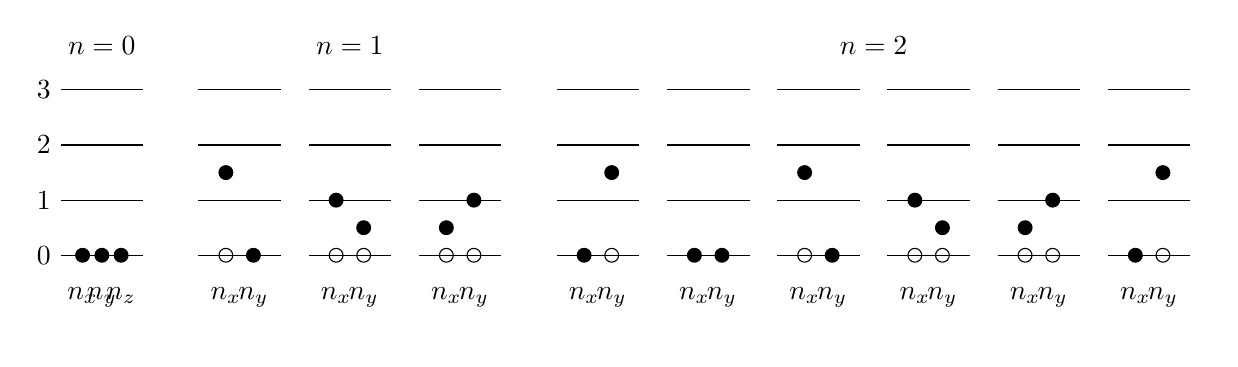
\begin{tikzpicture}[scale=0.35]
		\begin{scope}
		\foreach \i in {0,...,3}
		{
			\draw (-1,2*\i) node[anchor=east] {$\i$} --(2,2*\i);
		}
		\filldraw (-0.2,0) node[anchor=north,inner sep=.4cm] {$n_x$} circle (0.25cm); 
		\filldraw (0.5,0) node[anchor=north,inner sep=.4cm] {$n_y$} circle (0.25cm);
		\filldraw (1.2,0) node[anchor=north,inner sep=.4cm] {$n_z$} circle (0.25cm);
		\node[] at (0.5,7.6) {$n=0$};
		\end{scope}
		\begin{scope}[xshift=5cm]
		\foreach \i in {0,...,3}
		{
			\draw (-1,2*\i) --(2,2*\i);
		}
		\draw (0,0) node[anchor=north,inner sep=.4cm] {$n_x$} circle (0.25cm); 
		\filldraw (1,0) node[anchor=north,inner sep=.4cm] {$n_y$} circle (0.25cm);
		\filldraw (0,3) circle (0.25cm);
		\end{scope}
		\begin{scope}[xshift=9cm]
		\foreach \i in {0,...,3}
		{
			\draw (-1,2*\i) --(2,2*\i);
		}
		\draw (0,0) node[anchor=north,inner sep=.4cm] {$n_x$} circle (0.25cm); 
		\draw (1,0) node[anchor=north,inner sep=.4cm] {$n_y$} circle (0.25cm);
		\filldraw (0,2) circle (0.25cm); 
		\filldraw (1,1) circle (0.25cm); 
		\node[] at (0.5,7.6) {$n=1$};
		\end{scope}
		\begin{scope}[xshift=13cm]
		\foreach \i in {0,...,3}
		{
			\draw (-1,2*\i) --(2,2*\i);
		}
		\draw (0,0) node[anchor=north,inner sep=.4cm] {$n_x$} circle (0.25cm); 
		\draw (1,0) node[anchor=north,inner sep=.4cm] {$n_y$} circle (0.25cm);
		\filldraw (0,1) circle (0.25cm); 
		\filldraw (1,2) circle (0.25cm); 
		\end{scope}
		\begin{scope}[xshift=18cm]
		\foreach \i in {0,...,3}
		{
			\draw (-1,2*\i) --(2,2*\i);
		}
		\filldraw (0,0) node[anchor=north,inner sep=.4cm] {$n_x$} circle (0.25cm); 
		\draw (1,0) node[anchor=north,inner sep=.4cm] {$n_y$} circle (0.25cm);
		\filldraw (1,3) circle (0.25cm); 
		\end{scope}
		\begin{scope}[xshift=22cm]
		\foreach \i in {0,...,3}
		{
			\draw (-1,2*\i) --(2,2*\i);
		}
		\filldraw (0,0) node[anchor=north,inner sep=.4cm] {$n_x$} circle (0.25cm); 
		\filldraw (1,0) node[anchor=north,inner sep=.4cm] {$n_y$} circle (0.25cm);
		\end{scope}
		\begin{scope}[xshift=26cm]
		\foreach \i in {0,...,3}
		{
			\draw (-1,2*\i) --(2,2*\i);
		}
		\draw (0,0) node[anchor=north,inner sep=.4cm] {$n_x$} circle (0.25cm); 
		\filldraw (1,0) node[anchor=north,inner sep=.4cm] {$n_y$} circle (0.25cm);
		\filldraw (0,3) circle (0.25cm);
		\node[] at (2.5,7.6) {$n=2$};
		\end{scope}
		\begin{scope}[xshift=30cm]
		\foreach \i in {0,...,3}
		{
			\draw (-1,2*\i) --(2,2*\i);
		}
		\draw (0,0) node[anchor=north,inner sep=.4cm] {$n_x$} circle (0.25cm); 
		\draw (1,0) node[anchor=north,inner sep=.4cm] {$n_y$} circle (0.25cm);
		\filldraw (0,2) circle (0.25cm); 
		\filldraw (1,1) circle (0.25cm); 
		\end{scope}
		\begin{scope}[xshift=34cm]
		\foreach \i in {0,...,3}
		{
			\draw (-1,2*\i) --(2,2*\i);
		}
		\draw (0,0) node[anchor=north,inner sep=.4cm] {$n_x$} circle (0.25cm); 
		\draw (1,0) node[anchor=north,inner sep=.4cm] {$n_y$} circle (0.25cm);
		\filldraw (0,1) circle (0.25cm); 
		\filldraw (1,2) circle (0.25cm); 
		\end{scope}
		\begin{scope}[xshift=38cm]
		\foreach \i in {0,...,3}
		{
			\draw (-1,2*\i) --(2,2*\i);
		}
		\filldraw (0,0) node[anchor=north,inner sep=.4cm] {$n_x$} circle (0.25cm); 
		\draw (1,0) node[anchor=north,inner sep=.4cm] {$n_y$} circle (0.25cm);
		\filldraw (1,3) circle (0.25cm); 
		\end{scope}
		\end{tikzpicture}
	\end{center}

	\begin{center}
		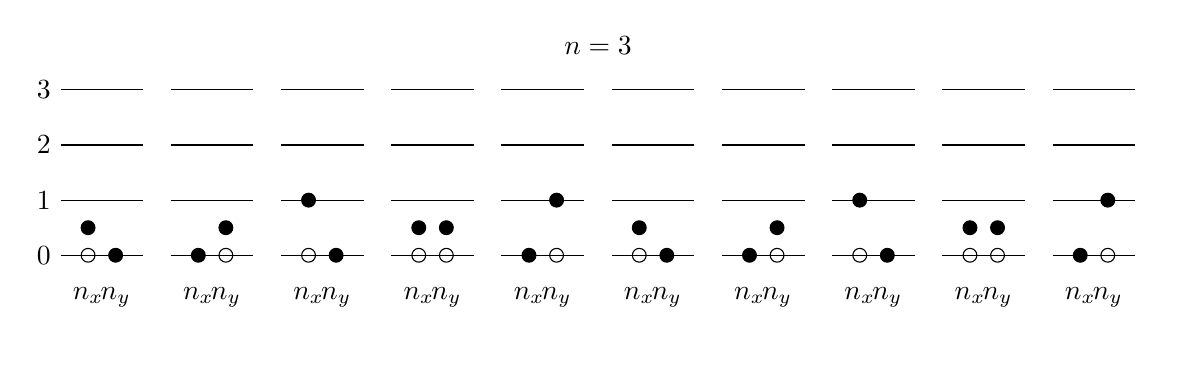
\begin{tikzpicture}[scale=0.35]
		\begin{scope}
		\foreach \i in {0,...,3}
		{
			\draw (-1,2*\i) node[anchor=east] {$\i$} --(2,2*\i);
		}
		\draw (0,0) node[anchor=north,inner sep=.4cm] {$n_x$} circle (0.25cm); 
		\filldraw (1,0) node[anchor=north,inner sep=.4cm] {$n_y$} circle (0.25cm);
		\filldraw (0,1) circle (0.25cm);
		\end{scope}
		\begin{scope}[xshift=4cm]
		\foreach \i in {0,...,3}
		{
			\draw (-1,2*\i) --(2,2*\i);
		}
		\filldraw (0,0) node[anchor=north,inner sep=.4cm] {$n_x$} circle (0.25cm); 
		\draw (1,0) node[anchor=north,inner sep=.4cm] {$n_y$} circle (0.25cm);
		\filldraw (1,1) circle (0.25cm); 
		\end{scope}
		\begin{scope}[xshift=8cm]
		\foreach \i in {0,...,3}
		{
			\draw (-1,2*\i) --(2,2*\i);
		}
		\draw (0,0) node[anchor=north,inner sep=.4cm] {$n_x$} circle (0.25cm); 
		\filldraw (1,0) node[anchor=north,inner sep=.4cm] {$n_y$} circle (0.25cm);
		\filldraw (0,2) circle (0.25cm);
		\end{scope}
		\begin{scope}[xshift=12cm]
		\foreach \i in {0,...,3}
		{
			\draw (-1,2*\i) --(2,2*\i);
		}
		\draw (0,0) node[anchor=north,inner sep=.4cm] {$n_x$} circle (0.25cm); 
		\draw (1,0) node[anchor=north,inner sep=.4cm] {$n_y$} circle (0.25cm);
		\filldraw (0,1) circle (0.25cm); 
		\filldraw (1,1) circle (0.25cm);
		\end{scope}
		\begin{scope}[xshift=16cm]
		\foreach \i in {0,...,3}
		{
			\draw (-1,2*\i) --(2,2*\i);
		}
		\filldraw (0,0) node[anchor=north,inner sep=.4cm] {$n_x$} circle (0.25cm); 
		\draw (1,0) node[anchor=north,inner sep=.4cm] {$n_y$} circle (0.25cm); 
		\filldraw (1,2) circle (0.25cm);
		\node[] at (2.5,7.6) {$n=3$};
		\end{scope}
		\begin{scope}[xshift=20cm]
		\foreach \i in {0,...,3}
		{
			\draw (-1,2*\i) --(2,2*\i);
		}
		\draw (0,0) node[anchor=north,inner sep=.4cm] {$n_x$} circle (0.25cm); 
		\filldraw (1,0) node[anchor=north,inner sep=.4cm] {$n_y$} circle (0.25cm);
		\filldraw (0,1) circle (0.25cm);
		\end{scope}
		\begin{scope}[xshift=24cm]
		\foreach \i in {0,...,3}
		{
			\draw (-1,2*\i) --(2,2*\i);
		}
		\filldraw (0,0) node[anchor=north,inner sep=.4cm] {$n_x$} circle (0.25cm); 
		\draw (1,0) node[anchor=north,inner sep=.4cm] {$n_y$} circle (0.25cm);
		\filldraw (1,1) circle (0.25cm); 
		\end{scope}
		\begin{scope}[xshift=28cm]
		\foreach \i in {0,...,3}
		{
			\draw (-1,2*\i) --(2,2*\i);
		}
		\draw (0,0) node[anchor=north,inner sep=.4cm] {$n_x$} circle (0.25cm); 
		\filldraw (1,0) node[anchor=north,inner sep=.4cm] {$n_y$} circle (0.25cm);
		\filldraw (0,2) circle (0.25cm);
		\end{scope}
		\begin{scope}[xshift=32cm]
		\foreach \i in {0,...,3}
		{
			\draw (-1,2*\i) --(2,2*\i);
		}
		\draw (0,0) node[anchor=north,inner sep=.4cm] {$n_x$} circle (0.25cm); 
		\draw (1,0) node[anchor=north,inner sep=.4cm] {$n_y$} circle (0.25cm);
		\filldraw (0,1) circle (0.25cm); 
		\filldraw (1,1) circle (0.25cm);
		\end{scope}
		\begin{scope}[xshift=36cm]
		\foreach \i in {0,...,3}
		{
			\draw (-1,2*\i) --(2,2*\i);
		}
		\filldraw (0,0) node[anchor=north,inner sep=.4cm] {$n_x$} circle (0.25cm); 
		\draw (1,0) node[anchor=north,inner sep=.4cm] {$n_y$} circle (0.25cm); 
		\filldraw (1,2) circle (0.25cm);
		\end{scope}
		\end{tikzpicture}
	\end{center}
	\caption{Possible states of a three dimensional harmonic oscillator.}
	\label{fig:schematic_3d}
\end{figure}

\section{Quantum double dots} \label{sec:doubledots}
Another historically important quantum system is the double dot, which similarly to the single dot can be solved analytically. For the same reason as the single dot often is called an artificial atom, the double dots are called artificial molecules. 

The potential of symmetrical quantum dots can in principle have a variety of different shapes, but the most used one-dimensional potentials can be derived from
\begin{equation}
V_i(x)=\frac{1}{2}\omega^2\bigg[|x_i|^a-\Big(\frac{b}{2}\Big)^a\bigg]^2
\label{eq:doublewell}
\end{equation}
with $b$ as the distance between the bottoms of the wells and $a$ as an arbitrary integer \cite{jelic_double_2012}. Setting $a=1$ gives two parabolic wells with a sharp local maximum at $x=0$, while $a=2$ gives a smoother but steeper well. In figure \eqref{fig:doublewell} the potential is plotted for $a=1,2$ and $3$.

\begin{figure}
	\centering
	% This file was created by matplotlib2tikz v0.7.4.
\begin{tikzpicture}

\begin{axis}[
legend cell align={left},
legend style={at={(0.5,0.91)}, anchor=north, draw=white!80.0!black},
%axis background/.style={fill=white!89.80392156862746!black},
axis line style={black},
tick align=outside,
tick pos=left,
%x grid style={black},
xlabel={$x$},
xmajorgrids,
xmin=-3.2, xmax=3.2,
xtick style={color=black},
%y grid style={black},
ylabel={$V_i^{\text{DW}}(x)$},
ymajorgrids,
ymin=0, ymax=8,
ytick style={color=black}
]
\addplot [thick, color0]
table {%
-3 8
-2.99399399399399 7.95202409616824
-2.98798798798799 7.90419248076906
-2.98198198198198 7.85650515380245
-2.97597597597598 7.80896211526842
-2.96996996996997 7.76156336516697
-2.96396396396396 7.71430890349809
-2.95795795795796 7.66719873026179
-2.95195195195195 7.62023284545807
-2.94594594594595 7.57341124908693
-2.93993993993994 7.52673394114836
-2.93393393393393 7.48020092164236
-2.92792792792793 7.43381219056895
-2.92192192192192 7.38756774792811
-2.91591591591592 7.34146759371985
-2.90990990990991 7.29551172794416
-2.9039039039039 7.24970015060105
-2.8978978978979 7.20403286169052
-2.89189189189189 7.15850986121257
-2.88588588588589 7.11313114916719
-2.87987987987988 7.06789672555438
-2.87387387387387 7.02280659037416
-2.86786786786787 6.97786074362651
-2.86186186186186 6.93305918531144
-2.85585585585586 6.88840191542894
-2.84984984984985 6.84388893397902
-2.84384384384384 6.79952024096168
-2.83783783783784 6.75529583637692
-2.83183183183183 6.71121572022473
-2.82582582582583 6.66727989250512
-2.81981981981982 6.62348835321808
-2.81381381381381 6.57984110236362
-2.80780780780781 6.53633813994174
-2.8018018018018 6.49297946595244
-2.7957957957958 6.44976508039571
-2.78978978978979 6.40669498327156
-2.78378378378378 6.36376917457999
-2.77777777777778 6.32098765432099
-2.77177177177177 6.27835042249457
-2.76576576576577 6.23585747910072
-2.75975975975976 6.19350882413946
-2.75375375375375 6.15130445761076
-2.74774774774775 6.10924437951465
-2.74174174174174 6.06732858985111
-2.73573573573574 6.02555708862015
-2.72972972972973 5.98392987582177
-2.72372372372372 5.94244695145596
-2.71771771771772 5.90110831552273
-2.71171171171171 5.85991396802207
-2.70570570570571 5.818863908954
-2.6996996996997 5.7779581383185
-2.69369369369369 5.73719665611558
-2.68768768768769 5.69657946234523
-2.68168168168168 5.65610655700746
-2.67567567567568 5.61577794010226
-2.66966966966967 5.57559361162965
-2.66366366366366 5.53555357158961
-2.65765765765766 5.49565781998214
-2.65165165165165 5.45590635680726
-2.64564564564565 5.41629918206495
-2.63963963963964 5.37683629575522
-2.63363363363363 5.33751769787806
-2.62762762762763 5.29834338843348
-2.62162162162162 5.25931336742147
-2.61561561561562 5.22042763484205
-2.60960960960961 5.1816861906952
-2.6036036036036 5.14308903498093
-2.5975975975976 5.10463616769923
-2.59159159159159 5.06632758885011
-2.58558558558559 5.02816329843357
-2.57957957957958 4.9901432964496
-2.57357357357357 4.95226758289821
-2.56756756756757 4.9145361577794
-2.56156156156156 4.87694902109316
-2.55555555555556 4.8395061728395
-2.54954954954955 4.80220761301842
-2.54354354354354 4.76505334162992
-2.53753753753754 4.72804335867399
-2.53153153153153 4.69117766415064
-2.52552552552553 4.65445625805986
-2.51951951951952 4.61787914040166
-2.51351351351351 4.58144631117604
-2.50750750750751 4.545157770383
-2.5015015015015 4.50901351802253
-2.4954954954955 4.47301355409463
-2.48948948948949 4.43715787859932
-2.48348348348348 4.40144649153658
-2.47747747747748 4.36587939290642
-2.47147147147147 4.33045658270883
-2.46546546546547 4.29517806094383
-2.45945945945946 4.2600438276114
-2.45345345345345 4.22505388271154
-2.44744744744745 4.19020822624426
-2.44144144144144 4.15550685820956
-2.43543543543544 4.12094977860743
-2.42942942942943 4.08653698743789
-2.42342342342342 4.05226848470092
-2.41741741741742 4.01814427039652
-2.41141141141141 3.9841643445247
-2.40540540540541 3.95032870708546
-2.3993993993994 3.9166373580788
-2.39339339339339 3.88309029750471
-2.38738738738739 3.8496875253632
-2.38138138138138 3.81642904165427
-2.37537537537538 3.78331484637791
-2.36936936936937 3.75034493953413
-2.36336336336336 3.71751932112293
-2.35735735735736 3.6848379911443
-2.35135135135135 3.65230094959825
-2.34534534534535 3.61990819648477
-2.33933933933934 3.58765973180388
-2.33333333333333 3.55555555555556
-2.32732732732733 3.52359566773981
-2.32132132132132 3.49178006835664
-2.31531531531532 3.46010875740605
-2.30930930930931 3.42858173488804
-2.3033033033033 3.39719900080261
-2.2972972972973 3.36596055514974
-2.29129129129129 3.33486639792946
-2.28528528528529 3.30391652914175
-2.27927927927928 3.27311094878663
-2.27327327327327 3.24244965686407
-2.26726726726727 3.2119326533741
-2.26126126126126 3.1815599383167
-2.25525525525526 3.15133151169187
-2.24924924924925 3.12124737349963
-2.24324324324324 3.09130752373995
-2.23723723723724 3.06151196241286
-2.23123123123123 3.03186068951835
-2.22522522522523 3.00235370505641
-2.21921921921922 2.97299100902705
-2.21321321321321 2.94377260143026
-2.20720720720721 2.91469848226605
-2.2012012012012 2.88576865153442
-2.1951951951952 2.85698310923536
-2.18918918918919 2.82834185536888
-2.18318318318318 2.79984488993498
-2.17717717717718 2.77149221293365
-2.17117117117117 2.74328382436491
-2.16516516516517 2.71521972422873
-2.15915915915916 2.68729991252514
-2.15315315315315 2.65952438925412
-2.14714714714715 2.63189315441568
-2.14114114114114 2.60440620800981
-2.13513513513514 2.57706355003652
-2.12912912912913 2.54986518049581
-2.12312312312312 2.52281109938767
-2.11711711711712 2.49590130671212
-2.11111111111111 2.46913580246914
-2.10510510510511 2.44251458665873
-2.0990990990991 2.4160376592809
-2.09309309309309 2.38970502033565
-2.08708708708709 2.36351666982298
-2.08108108108108 2.33747260774288
-2.07507507507508 2.31157283409536
-2.06906906906907 2.28581734888041
-2.06306306306306 2.26020615209804
-2.05705705705706 2.23473924374825
-2.05105105105105 2.20941662383104
-2.04504504504505 2.1842382923464
-2.03903903903904 2.15920424929434
-2.03303303303303 2.13431449467485
-2.02702702702703 2.10956902848795
-2.02102102102102 2.08496785073362
-2.01501501501502 2.06051096141186
-2.00900900900901 2.03619836052268
-2.003003003003 2.01203004806608
-1.996996996997 1.98800602404206
-1.99099099099099 1.96412628845061
-1.98498498498498 1.94039084129174
-1.97897897897898 1.91679968256545
-1.97297297297297 1.89335281227173
-1.96696696696697 1.87005023041059
-1.96096096096096 1.84689193698203
-1.95495495495495 1.82387793198604
-1.94894894894895 1.80100821542263
-1.94294294294294 1.7782827872918
-1.93693693693694 1.75570164759354
-1.93093093093093 1.73326479632786
-1.92492492492492 1.71097223349476
-1.91891891891892 1.68882395909423
-1.91291291291291 1.66681997312628
-1.90690690690691 1.64496027559091
-1.9009009009009 1.62324486648811
-1.89489489489489 1.60167374581789
-1.88888888888889 1.58024691358025
-1.88288288288288 1.55896436977518
-1.87687687687688 1.53782611440269
-1.87087087087087 1.51683214746278
-1.86486486486486 1.49598246895544
-1.85885885885886 1.47527707888068
-1.85285285285285 1.4547159772385
-1.84684684684685 1.43429916402889
-1.84084084084084 1.41402663925186
-1.83483483483483 1.39389840290741
-1.82882882882883 1.37391445499554
-1.82282282282282 1.35407479551624
-1.81681681681682 1.33437942446951
-1.81081081081081 1.31482834185537
-1.8048048048048 1.2954215476738
-1.7987987987988 1.27615904192481
-1.79279279279279 1.25704082460839
-1.78678678678679 1.23806689572455
-1.78078078078078 1.21923725527329
-1.77477477477477 1.20055190325461
-1.76876876876877 1.1820108396685
-1.76276276276276 1.16361406451497
-1.75675675675676 1.14536157779401
-1.75075075075075 1.12725337950563
-1.74474474474474 1.10928946964983
-1.73873873873874 1.0914698482266
-1.73273273273273 1.07379451523596
-1.72672672672673 1.05626347067789
-1.72072072072072 1.03887671455239
-1.71471471471471 1.02163424685947
-1.70870870870871 1.00453606759913
-1.7027027027027 0.987582176771366
-1.6966966966967 0.970772574376178
-1.69069069069069 0.954107260413567
-1.68468468468468 0.937586234883532
-1.67867867867868 0.921209497786074
-1.67267267267267 0.904977049121193
-1.66666666666667 0.888888888888889
-1.66066066066066 0.872945017089161
-1.65465465465465 0.857145433722011
-1.64864864864865 0.841490138787436
-1.64264264264264 0.825979132285439
-1.63663663663664 0.810612414216018
-1.63063063063063 0.795389984579174
-1.62462462462462 0.780311843374906
-1.61861861861862 0.765377990603216
-1.61261261261261 0.750588426264102
-1.60660660660661 0.735943150357565
-1.6006006006006 0.721442162883604
-1.59459459459459 0.70708546384222
-1.58858858858859 0.692873053233414
-1.58258258258258 0.678804931057183
-1.57657657657658 0.66488109731353
-1.57057057057057 0.651101552002453
-1.56456456456456 0.637466295123953
-1.55855855855856 0.62397532667803
-1.55255255255255 0.610628646664683
-1.54654654654655 0.597426255083913
-1.54054054054054 0.58436815193572
-1.53453453453453 0.571454337220103
-1.52852852852853 0.558684810937063
-1.52252252252252 0.5460595730866
-1.51651651651652 0.533578623668714
-1.51051051051051 0.521241962683404
-1.5045045045045 0.509049590130671
-1.4984984984985 0.497001506010515
-1.49249249249249 0.485097710322936
-1.48648648648649 0.473338203067933
-1.48048048048048 0.461722984245507
-1.47447447447447 0.450252053855657
-1.46846846846847 0.438925411898385
-1.46246246246246 0.427743058373689
-1.45645645645646 0.41670499328157
-1.45045045045045 0.405811216622028
-1.44444444444444 0.395061728395062
-1.43843843843844 0.384456528600673
-1.43243243243243 0.373995617238861
-1.42642642642643 0.363678994309625
-1.42042042042042 0.353506659812966
-1.41441441441441 0.343478613748884
-1.40840840840841 0.333594856117379
-1.4024024024024 0.32385538691845
-1.3963963963964 0.314260206152098
-1.39039039039039 0.304809313818323
-1.38438438438438 0.295502709917124
-1.37837837837838 0.286340394448502
-1.37237237237237 0.277322367412458
-1.36636636636637 0.268448628808989
-1.36036036036036 0.259719178638098
-1.35435435435435 0.251134016899783
-1.34834834834835 0.242693143594044
-1.34234234234234 0.234396558720883
-1.33633633633634 0.226244262280298
-1.33033033033033 0.21823625427229
-1.32432432432432 0.210372534696859
-1.31831831831832 0.202653103554004
-1.31231231231231 0.195077960843727
-1.30630630630631 0.187647106566025
-1.3003003003003 0.180360540720901
-1.29429429429429 0.173218263308353
-1.28828828828829 0.166220274328382
-1.28228228228228 0.159366573780988
-1.27627627627628 0.152657161666171
-1.27027027027027 0.14609203798393
-1.26426426426426 0.139671202734266
-1.25825825825826 0.133394655917178
-1.25225225225225 0.127262397532668
-1.24624624624625 0.121274427580734
-1.24024024024024 0.115430746061377
-1.23423423423423 0.109731352974596
-1.22822822822823 0.104176248320392
-1.22222222222222 0.0987654320987655
-1.21621621621622 0.0934989043097151
-1.21021021021021 0.0883766649532415
-1.2042042042042 0.0833987140293447
-1.1981981981982 0.0785650515380245
-1.19219219219219 0.0738756774792812
-1.18618618618619 0.0693305918531144
-1.18018018018018 0.0649297946595243
-1.17417417417417 0.0606732858985112
-1.16816816816817 0.0565610655700746
-1.16216216216216 0.0525931336742148
-1.15615615615616 0.0487694902109317
-1.15015015015015 0.0450901351802252
-1.14414414414414 0.0415550685820957
-1.13813813813814 0.0381642904165427
-1.13213213213213 0.0349178006835664
-1.12612612612613 0.031815599383167
-1.12012012012012 0.0288576865153442
-1.11411411411411 0.0260440620800982
-1.10810810810811 0.0233747260774288
-1.1021021021021 0.0208496785073361
-1.0960960960961 0.0184689193698203
-1.09009009009009 0.0162324486648811
-1.08408408408408 0.0141402663925187
-1.07807807807808 0.0121923725527329
-1.07207207207207 0.0103887671455239
-1.06606606606607 0.00872945017089163
-1.06006006006006 0.00721442162883604
-1.05405405405405 0.00584368151935722
-1.04804804804805 0.00461722984245507
-1.04204204204204 0.00353506659812965
-1.03603603603604 0.00259719178638099
-1.03003003003003 0.00180360540720901
-1.02402402402402 0.00115430746061378
-1.01801801801802 0.000649297946595247
-1.01201201201201 0.000288576865153439
-1.00600600600601 7.21442162883625e-05
-1 0
-0.993993993993994 7.21442162883625e-05
-0.987987987987988 0.00028857686515345
-0.981981981981982 0.000649297946595231
-0.975975975975976 0.00115430746061376
-0.96996996996997 0.00180360540720901
-0.963963963963964 0.00259719178638099
-0.957957957957958 0.00353506659812969
-0.951951951951952 0.00461722984245503
-0.945945945945946 0.00584368151935717
-0.93993993993994 0.00721442162883604
-0.933933933933934 0.00872945017089163
-0.927927927927928 0.0103887671455239
-0.921921921921922 0.0121923725527328
-0.915915915915916 0.0141402663925186
-0.90990990990991 0.0162324486648811
-0.903903903903904 0.0184689193698203
-0.897897897897898 0.0208496785073362
-0.891891891891892 0.0233747260774287
-0.885885885885886 0.0260440620800981
-0.87987987987988 0.0288576865153442
-0.873873873873874 0.031815599383167
-0.867867867867868 0.0349178006835665
-0.861861861861862 0.0381642904165425
-0.855855855855856 0.0415550685820955
-0.84984984984985 0.0450901351802252
-0.843843843843844 0.0487694902109317
-0.837837837837838 0.0525931336742148
-0.831831831831832 0.0565610655700744
-0.825825825825826 0.060673285898511
-0.81981981981982 0.0649297946595243
-0.813813813813814 0.0693305918531144
-0.807807807807808 0.0738756774792812
-0.801801801801802 0.0785650515380247
-0.795795795795796 0.0833987140293445
-0.78978978978979 0.0883766649532415
-0.783783783783784 0.0934989043097151
-0.777777777777778 0.0987654320987655
-0.771771771771772 0.104176248320393
-0.765765765765766 0.109731352974596
-0.75975975975976 0.115430746061377
-0.753753753753754 0.121274427580734
-0.747747747747748 0.127262397532668
-0.741741741741742 0.133394655917179
-0.735735735735736 0.139671202734266
-0.72972972972973 0.14609203798393
-0.723723723723724 0.152657161666171
-0.717717717717718 0.159366573780988
-0.711711711711712 0.166220274328383
-0.705705705705706 0.173218263308353
-0.6996996996997 0.180360540720901
-0.693693693693694 0.187647106566025
-0.687687687687688 0.195077960843727
-0.681681681681682 0.202653103554005
-0.675675675675676 0.210372534696859
-0.66966966966967 0.21823625427229
-0.663663663663664 0.226244262280298
-0.657657657657658 0.234396558720883
-0.651651651651652 0.242693143594045
-0.645645645645646 0.251134016899782
-0.63963963963964 0.259719178638097
-0.633633633633634 0.268448628808989
-0.627627627627628 0.277322367412458
-0.621621621621621 0.286340394448503
-0.615615615615616 0.295502709917124
-0.60960960960961 0.304809313818323
-0.603603603603604 0.314260206152098
-0.597597597597598 0.32385538691845
-0.591591591591591 0.333594856117379
-0.585585585585586 0.343478613748884
-0.57957957957958 0.353506659812966
-0.573573573573574 0.363678994309625
-0.567567567567568 0.373995617238861
-0.561561561561561 0.384456528600673
-0.555555555555555 0.395061728395062
-0.54954954954955 0.405811216622027
-0.543543543543544 0.41670499328157
-0.537537537537538 0.427743058373689
-0.531531531531531 0.438925411898385
-0.525525525525525 0.450252053855658
-0.51951951951952 0.461722984245506
-0.513513513513514 0.473338203067933
-0.507507507507508 0.485097710322936
-0.501501501501501 0.497001506010515
-0.495495495495495 0.509049590130672
-0.48948948948949 0.521241962683404
-0.483483483483484 0.533578623668714
-0.477477477477477 0.5460595730866
-0.471471471471471 0.558684810937063
-0.465465465465465 0.571454337220103
-0.45945945945946 0.584368151935719
-0.453453453453454 0.597426255083913
-0.447447447447447 0.610628646664683
-0.441441441441441 0.62397532667803
-0.435435435435435 0.637466295123953
-0.42942942942943 0.651101552002452
-0.423423423423424 0.66488109731353
-0.417417417417417 0.678804931057183
-0.411411411411411 0.692873053233414
-0.405405405405405 0.707085463842221
-0.3993993993994 0.721442162883604
-0.393393393393394 0.735943150357564
-0.387387387387387 0.750588426264102
-0.381381381381381 0.765377990603216
-0.375375375375375 0.780311843374907
-0.36936936936937 0.795389984579173
-0.363363363363364 0.810612414216017
-0.357357357357357 0.825979132285439
-0.351351351351351 0.841490138787436
-0.345345345345345 0.857145433722011
-0.33933933933934 0.872945017089161
-0.333333333333333 0.888888888888889
-0.327327327327327 0.904977049121193
-0.321321321321321 0.921209497786074
-0.315315315315315 0.937586234883532
-0.30930930930931 0.954107260413566
-0.303303303303303 0.970772574376178
-0.297297297297297 0.987582176771366
-0.291291291291291 1.00453606759913
-0.285285285285285 1.02163424685947
-0.279279279279279 1.03887671455239
-0.273273273273273 1.05626347067788
-0.267267267267267 1.07379451523596
-0.261261261261261 1.0914698482266
-0.255255255255255 1.10928946964983
-0.249249249249249 1.12725337950563
-0.243243243243243 1.14536157779401
-0.237237237237237 1.16361406451497
-0.231231231231231 1.1820108396685
-0.225225225225225 1.20055190325461
-0.219219219219219 1.21923725527329
-0.213213213213213 1.23806689572455
-0.207207207207207 1.25704082460839
-0.201201201201201 1.27615904192481
-0.195195195195195 1.2954215476738
-0.189189189189189 1.31482834185537
-0.183183183183183 1.33437942446951
-0.177177177177177 1.35407479551624
-0.171171171171171 1.37391445499554
-0.165165165165165 1.39389840290741
-0.159159159159159 1.41402663925187
-0.153153153153153 1.43429916402889
-0.147147147147147 1.4547159772385
-0.141141141141141 1.47527707888068
-0.135135135135135 1.49598246895544
-0.129129129129129 1.51683214746278
-0.123123123123123 1.53782611440269
-0.117117117117117 1.55896436977518
-0.111111111111111 1.58024691358025
-0.105105105105105 1.60167374581789
-0.099099099099099 1.62324486648811
-0.0930930930930933 1.64496027559091
-0.0870870870870872 1.66681997312628
-0.0810810810810811 1.68882395909423
-0.075075075075075 1.71097223349476
-0.069069069069069 1.73326479632786
-0.0630630630630633 1.75570164759354
-0.0570570570570572 1.7782827872918
-0.0510510510510511 1.80100821542263
-0.045045045045045 1.82387793198604
-0.0390390390390389 1.84689193698203
-0.0330330330330328 1.87005023041059
-0.0270270270270272 1.89335281227173
-0.0210210210210211 1.91679968256545
-0.015015015015015 1.94039084129174
-0.00900900900900892 1.96412628845061
-0.00300300300300282 1.98800602404206
0.00300300300300282 1.98800602404206
0.00900900900900892 1.96412628845061
0.015015015015015 1.94039084129174
0.0210210210210211 1.91679968256545
0.0270270270270272 1.89335281227173
0.0330330330330328 1.87005023041059
0.0390390390390389 1.84689193698203
0.045045045045045 1.82387793198604
0.0510510510510511 1.80100821542263
0.0570570570570572 1.7782827872918
0.0630630630630629 1.75570164759354
0.069069069069069 1.73326479632786
0.075075075075075 1.71097223349476
0.0810810810810811 1.68882395909423
0.0870870870870872 1.66681997312628
0.0930930930930929 1.64496027559091
0.099099099099099 1.62324486648811
0.105105105105105 1.60167374581789
0.111111111111111 1.58024691358025
0.117117117117117 1.55896436977518
0.123123123123123 1.53782611440269
0.129129129129129 1.51683214746278
0.135135135135135 1.49598246895544
0.141141141141141 1.47527707888068
0.147147147147147 1.4547159772385
0.153153153153153 1.43429916402889
0.159159159159159 1.41402663925187
0.165165165165165 1.39389840290741
0.171171171171171 1.37391445499554
0.177177177177177 1.35407479551624
0.183183183183183 1.33437942446952
0.189189189189189 1.31482834185537
0.195195195195195 1.2954215476738
0.201201201201201 1.27615904192481
0.207207207207207 1.25704082460839
0.213213213213213 1.23806689572455
0.219219219219219 1.21923725527329
0.225225225225225 1.20055190325461
0.231231231231231 1.1820108396685
0.237237237237237 1.16361406451497
0.243243243243243 1.14536157779401
0.249249249249249 1.12725337950563
0.255255255255255 1.10928946964983
0.261261261261261 1.0914698482266
0.267267267267267 1.07379451523596
0.273273273273273 1.05626347067788
0.279279279279279 1.03887671455239
0.285285285285285 1.02163424685947
0.291291291291291 1.00453606759913
0.297297297297297 0.987582176771366
0.303303303303303 0.970772574376178
0.309309309309309 0.954107260413567
0.315315315315315 0.937586234883532
0.321321321321321 0.921209497786074
0.327327327327327 0.904977049121193
0.333333333333333 0.888888888888889
0.339339339339339 0.872945017089162
0.345345345345345 0.857145433722011
0.351351351351351 0.841490138787436
0.357357357357357 0.825979132285439
0.363363363363364 0.810612414216017
0.369369369369369 0.795389984579174
0.375375375375375 0.780311843374907
0.381381381381381 0.765377990603216
0.387387387387387 0.750588426264102
0.393393393393394 0.735943150357564
0.399399399399399 0.721442162883605
0.405405405405405 0.707085463842221
0.411411411411411 0.692873053233414
0.417417417417417 0.678804931057183
0.423423423423424 0.66488109731353
0.429429429429429 0.651101552002453
0.435435435435435 0.637466295123953
0.441441441441441 0.62397532667803
0.447447447447447 0.610628646664683
0.453453453453454 0.597426255083913
0.45945945945946 0.584368151935719
0.465465465465465 0.571454337220103
0.471471471471471 0.558684810937063
0.477477477477477 0.5460595730866
0.483483483483484 0.533578623668714
0.48948948948949 0.521241962683404
0.495495495495495 0.509049590130672
0.501501501501501 0.497001506010515
0.507507507507508 0.485097710322936
0.513513513513514 0.473338203067933
0.51951951951952 0.461722984245506
0.525525525525525 0.450252053855658
0.531531531531531 0.438925411898385
0.537537537537538 0.427743058373689
0.543543543543544 0.41670499328157
0.54954954954955 0.405811216622027
0.555555555555555 0.395061728395062
0.561561561561561 0.384456528600673
0.567567567567568 0.373995617238861
0.573573573573574 0.363678994309625
0.57957957957958 0.353506659812966
0.585585585585585 0.343478613748884
0.591591591591591 0.333594856117379
0.597597597597598 0.32385538691845
0.603603603603604 0.314260206152098
0.60960960960961 0.304809313818323
0.615615615615615 0.295502709917125
0.621621621621621 0.286340394448503
0.627627627627628 0.277322367412458
0.633633633633634 0.268448628808989
0.63963963963964 0.259719178638097
0.645645645645645 0.251134016899783
0.651651651651652 0.242693143594045
0.657657657657658 0.234396558720883
0.663663663663664 0.226244262280298
0.66966966966967 0.21823625427229
0.675675675675675 0.210372534696859
0.681681681681682 0.202653103554005
0.687687687687688 0.195077960843727
0.693693693693694 0.187647106566025
0.6996996996997 0.180360540720901
0.705705705705705 0.173218263308354
0.711711711711712 0.166220274328383
0.717717717717718 0.159366573780988
0.723723723723724 0.152657161666171
0.72972972972973 0.14609203798393
0.735735735735736 0.139671202734266
0.741741741741742 0.133394655917179
0.747747747747748 0.127262397532668
0.753753753753754 0.121274427580734
0.75975975975976 0.115430746061377
0.765765765765766 0.109731352974596
0.771771771771772 0.104176248320393
0.777777777777778 0.0987654320987655
0.783783783783784 0.0934989043097151
0.78978978978979 0.0883766649532415
0.795795795795796 0.0833987140293445
0.801801801801802 0.0785650515380247
0.807807807807808 0.0738756774792812
0.813813813813814 0.0693305918531144
0.81981981981982 0.0649297946595243
0.825825825825826 0.060673285898511
0.831831831831832 0.0565610655700747
0.837837837837838 0.0525931336742148
0.843843843843844 0.0487694902109317
0.84984984984985 0.0450901351802252
0.855855855855856 0.0415550685820955
0.861861861861862 0.0381642904165428
0.867867867867868 0.0349178006835665
0.873873873873874 0.031815599383167
0.87987987987988 0.0288576865153442
0.885885885885886 0.0260440620800981
0.891891891891892 0.0233747260774289
0.897897897897898 0.0208496785073362
0.903903903903904 0.0184689193698203
0.90990990990991 0.0162324486648811
0.915915915915916 0.0141402663925186
0.921921921921922 0.012192372552733
0.927927927927928 0.0103887671455239
0.933933933933934 0.00872945017089163
0.93993993993994 0.00721442162883604
0.945945945945946 0.00584368151935717
0.951951951951952 0.00461722984245512
0.957957957957958 0.00353506659812969
0.963963963963964 0.00259719178638099
0.96996996996997 0.00180360540720901
0.975975975975976 0.00115430746061376
0.981981981981982 0.000649297946595231
0.987987987987988 0.00028857686515345
0.993993993993994 7.21442162883625e-05
1 0
1.00600600600601 7.21442162883518e-05
1.01201201201201 0.00028857686515345
1.01801801801802 0.000649297946595231
1.02402402402402 0.0011543074606138
1.03003003003003 0.00180360540720901
1.03603603603604 0.00259719178638092
1.04204204204204 0.00353506659812969
1.04804804804805 0.00461722984245503
1.05405405405405 0.00584368151935727
1.06006006006006 0.00721442162883604
1.06606606606607 0.00872945017089151
1.07207207207207 0.0103887671455239
1.07807807807808 0.0121923725527328
1.08408408408408 0.0141402663925188
1.09009009009009 0.0162324486648811
1.0960960960961 0.0184689193698201
1.1021021021021 0.0208496785073362
1.10810810810811 0.0233747260774287
1.11411411411411 0.0260440620800983
1.12012012012012 0.0288576865153442
1.12612612612613 0.0318155993831667
1.13213213213213 0.0349178006835665
1.13813813813814 0.0381642904165425
1.14414414414414 0.0415550685820958
1.15015015015015 0.0450901351802252
1.15615615615616 0.0487694902109314
1.16216216216216 0.0525931336742148
1.16816816816817 0.0565610655700744
1.17417417417417 0.0606732858985113
1.18018018018018 0.0649297946595243
1.18618618618619 0.0693305918531141
1.19219219219219 0.0738756774792812
1.1981981981982 0.0785650515380243
1.2042042042042 0.0833987140293449
1.21021021021021 0.0883766649532415
1.21621621621622 0.0934989043097147
1.22222222222222 0.0987654320987655
1.22822822822823 0.104176248320392
1.23423423423423 0.109731352974596
1.24024024024024 0.115430746061377
1.24624624624625 0.121274427580733
1.25225225225225 0.127262397532668
1.25825825825826 0.133394655917178
1.26426426426426 0.139671202734266
1.27027027027027 0.14609203798393
1.27627627627628 0.15265716166617
1.28228228228228 0.159366573780988
1.28828828828829 0.166220274328382
1.29429429429429 0.173218263308354
1.3003003003003 0.180360540720901
1.30630630630631 0.187647106566025
1.31231231231231 0.195077960843727
1.31831831831832 0.202653103554004
1.32432432432432 0.210372534696859
1.33033033033033 0.21823625427229
1.33633633633634 0.226244262280298
1.34234234234234 0.234396558720883
1.34834834834835 0.242693143594044
1.35435435435435 0.251134016899783
1.36036036036036 0.259719178638097
1.36636636636637 0.26844862880899
1.37237237237237 0.277322367412458
1.37837837837838 0.286340394448502
1.38438438438438 0.295502709917125
1.39039039039039 0.304809313818323
1.3963963963964 0.314260206152099
1.4024024024024 0.32385538691845
1.40840840840841 0.333594856117378
1.41441441441441 0.343478613748884
1.42042042042042 0.353506659812966
1.42642642642643 0.363678994309626
1.43243243243243 0.373995617238861
1.43843843843844 0.384456528600672
1.44444444444444 0.395061728395062
1.45045045045045 0.405811216622027
1.45645645645646 0.416704993281571
1.46246246246246 0.427743058373689
1.46846846846847 0.438925411898384
1.47447447447447 0.450252053855658
1.48048048048048 0.461722984245506
1.48648648648649 0.473338203067934
1.49249249249249 0.485097710322936
1.4984984984985 0.497001506010514
1.5045045045045 0.509049590130672
1.51051051051051 0.521241962683404
1.51651651651652 0.533578623668714
1.52252252252252 0.5460595730866
1.52852852852853 0.558684810937062
1.53453453453453 0.571454337220103
1.54054054054054 0.584368151935719
1.54654654654655 0.597426255083913
1.55255255255255 0.610628646664683
1.55855855855856 0.623975326678029
1.56456456456456 0.637466295123953
1.57057057057057 0.651101552002452
1.57657657657658 0.664881097313531
1.58258258258258 0.678804931057183
1.58858858858859 0.692873053233413
1.59459459459459 0.707085463842221
1.6006006006006 0.721442162883604
1.60660660660661 0.735943150357566
1.61261261261261 0.750588426264102
1.61861861861862 0.765377990603215
1.62462462462462 0.780311843374907
1.63063063063063 0.795389984579173
1.63663663663664 0.810612414216019
1.64264264264264 0.825979132285439
1.64864864864865 0.841490138787435
1.65465465465465 0.857145433722011
1.66066066066066 0.872945017089161
1.66666666666667 0.88888888888889
1.67267267267267 0.904977049121193
1.67867867867868 0.921209497786073
1.68468468468468 0.937586234883532
1.69069069069069 0.954107260413566
1.6966966966967 0.970772574376179
1.7027027027027 0.987582176771366
1.70870870870871 1.00453606759913
1.71471471471471 1.02163424685947
1.72072072072072 1.03887671455239
1.72672672672673 1.05626347067789
1.73273273273273 1.07379451523596
1.73873873873874 1.0914698482266
1.74474474474474 1.10928946964983
1.75075075075075 1.12725337950563
1.75675675675676 1.14536157779401
1.76276276276276 1.16361406451497
1.76876876876877 1.1820108396685
1.77477477477477 1.20055190325461
1.78078078078078 1.21923725527329
1.78678678678679 1.23806689572455
1.79279279279279 1.25704082460839
1.7987987987988 1.27615904192481
1.8048048048048 1.2954215476738
1.81081081081081 1.31482834185537
1.81681681681682 1.33437942446952
1.82282282282282 1.35407479551624
1.82882882882883 1.37391445499553
1.83483483483483 1.39389840290741
1.84084084084084 1.41402663925186
1.84684684684685 1.43429916402889
1.85285285285285 1.4547159772385
1.85885885885886 1.47527707888068
1.86486486486486 1.49598246895544
1.87087087087087 1.51683214746278
1.87687687687688 1.53782611440269
1.88288288288288 1.55896436977518
1.88888888888889 1.58024691358025
1.89489489489489 1.60167374581789
1.9009009009009 1.62324486648811
1.90690690690691 1.64496027559091
1.91291291291291 1.66681997312628
1.91891891891892 1.68882395909423
1.92492492492492 1.71097223349476
1.93093093093093 1.73326479632786
1.93693693693694 1.75570164759354
1.94294294294294 1.7782827872918
1.94894894894895 1.80100821542263
1.95495495495495 1.82387793198604
1.96096096096096 1.84689193698203
1.96696696696697 1.87005023041059
1.97297297297297 1.89335281227173
1.97897897897898 1.91679968256545
1.98498498498498 1.94039084129174
1.99099099099099 1.96412628845061
1.996996996997 1.98800602404206
2.003003003003 2.01203004806608
2.00900900900901 2.03619836052269
2.01501501501502 2.06051096141186
2.02102102102102 2.08496785073361
2.02702702702703 2.10956902848795
2.03303303303303 2.13431449467485
2.03903903903904 2.15920424929434
2.04504504504505 2.1842382923464
2.05105105105105 2.20941662383104
2.05705705705706 2.23473924374825
2.06306306306306 2.26020615209804
2.06906906906907 2.28581734888041
2.07507507507508 2.31157283409536
2.08108108108108 2.33747260774288
2.08708708708709 2.36351666982298
2.09309309309309 2.38970502033565
2.0990990990991 2.4160376592809
2.10510510510511 2.44251458665873
2.11111111111111 2.46913580246913
2.11711711711712 2.49590130671212
2.12312312312312 2.52281109938767
2.12912912912913 2.54986518049581
2.13513513513514 2.57706355003652
2.14114114114114 2.60440620800981
2.14714714714715 2.63189315441568
2.15315315315315 2.65952438925412
2.15915915915916 2.68729991252514
2.16516516516517 2.71521972422873
2.17117117117117 2.7432838243649
2.17717717717718 2.77149221293365
2.18318318318318 2.79984488993498
2.18918918918919 2.82834185536888
2.1951951951952 2.85698310923536
2.2012012012012 2.88576865153442
2.20720720720721 2.91469848226605
2.21321321321321 2.94377260143026
2.21921921921922 2.97299100902705
2.22522522522523 3.00235370505641
2.23123123123123 3.03186068951835
2.23723723723724 3.06151196241286
2.24324324324324 3.09130752373995
2.24924924924925 3.12124737349963
2.25525525525526 3.15133151169187
2.26126126126126 3.18155993831669
2.26726726726727 3.2119326533741
2.27327327327327 3.24244965686407
2.27927927927928 3.27311094878663
2.28528528528529 3.30391652914175
2.29129129129129 3.33486639792946
2.2972972972973 3.36596055514974
2.3033033033033 3.3971990008026
2.30930930930931 3.42858173488804
2.31531531531532 3.46010875740605
2.32132132132132 3.49178006835664
2.32732732732733 3.52359566773981
2.33333333333333 3.55555555555555
2.33933933933934 3.58765973180388
2.34534534534535 3.61990819648477
2.35135135135135 3.65230094959824
2.35735735735736 3.6848379911443
2.36336336336336 3.71751932112292
2.36936936936937 3.75034493953413
2.37537537537538 3.78331484637791
2.38138138138138 3.81642904165426
2.38738738738739 3.8496875253632
2.39339339339339 3.88309029750471
2.3993993993994 3.9166373580788
2.40540540540541 3.95032870708546
2.41141141141141 3.98416434452471
2.41741741741742 4.01814427039652
2.42342342342342 4.05226848470092
2.42942942942943 4.08653698743789
2.43543543543544 4.12094977860743
2.44144144144144 4.15550685820956
2.44744744744745 4.19020822624426
2.45345345345345 4.22505388271154
2.45945945945946 4.2600438276114
2.46546546546547 4.29517806094383
2.47147147147147 4.33045658270884
2.47747747747748 4.36587939290642
2.48348348348348 4.40144649153658
2.48948948948949 4.43715787859932
2.4954954954955 4.47301355409463
2.5015015015015 4.50901351802253
2.50750750750751 4.545157770383
2.51351351351351 4.58144631117604
2.51951951951952 4.61787914040166
2.52552552552553 4.65445625805986
2.53153153153153 4.69117766415064
2.53753753753754 4.72804335867399
2.54354354354354 4.76505334162992
2.54954954954955 4.80220761301842
2.55555555555556 4.8395061728395
2.56156156156156 4.87694902109317
2.56756756756757 4.9145361577794
2.57357357357357 4.95226758289821
2.57957957957958 4.9901432964496
2.58558558558559 5.02816329843357
2.59159159159159 5.06632758885011
2.5975975975976 5.10463616769923
2.6036036036036 5.14308903498092
2.60960960960961 5.1816861906952
2.61561561561562 5.22042763484205
2.62162162162162 5.25931336742148
2.62762762762763 5.29834338843348
2.63363363363363 5.33751769787806
2.63963963963964 5.37683629575522
2.64564564564565 5.41629918206495
2.65165165165165 5.45590635680726
2.65765765765766 5.49565781998214
2.66366366366366 5.53555357158961
2.66966966966967 5.57559361162965
2.67567567567568 5.61577794010226
2.68168168168168 5.65610655700746
2.68768768768769 5.69657946234523
2.69369369369369 5.73719665611557
2.6996996996997 5.7779581383185
2.70570570570571 5.818863908954
2.71171171171171 5.85991396802208
2.71771771771772 5.90110831552273
2.72372372372372 5.94244695145596
2.72972972972973 5.98392987582177
2.73573573573574 6.02555708862015
2.74174174174174 6.06732858985111
2.74774774774775 6.10924437951465
2.75375375375375 6.15130445761076
2.75975975975976 6.19350882413946
2.76576576576577 6.23585747910072
2.77177177177177 6.27835042249457
2.77777777777778 6.32098765432099
2.78378378378378 6.36376917457998
2.78978978978979 6.40669498327156
2.7957957957958 6.44976508039571
2.8018018018018 6.49297946595244
2.80780780780781 6.53633813994174
2.81381381381381 6.57984110236362
2.81981981981982 6.62348835321808
2.82582582582583 6.66727989250512
2.83183183183183 6.71121572022473
2.83783783783784 6.75529583637692
2.84384384384384 6.79952024096168
2.84984984984985 6.84388893397902
2.85585585585586 6.88840191542894
2.86186186186186 6.93305918531144
2.86786786786787 6.97786074362651
2.87387387387387 7.02280659037415
2.87987987987988 7.06789672555438
2.88588588588589 7.11313114916718
2.89189189189189 7.15850986121257
2.8978978978979 7.20403286169052
2.9039039039039 7.24970015060105
2.90990990990991 7.29551172794416
2.91591591591592 7.34146759371984
2.92192192192192 7.38756774792811
2.92792792792793 7.43381219056895
2.93393393393393 7.48020092164237
2.93993993993994 7.52673394114836
2.94594594594595 7.57341124908692
2.95195195195195 7.62023284545807
2.95795795795796 7.66719873026179
2.96396396396396 7.7143089034981
2.96996996996997 7.76156336516697
2.97597597597598 7.80896211526842
2.98198198198198 7.85650515380245
2.98798798798799 7.90419248076906
2.99399399399399 7.95202409616824
3 8
};
\addlegendentry{$a=1$}
\addplot [thick, color1]
table {%
-3 64
-2.99399399399399 63.4252965745565
-2.98798798798799 62.8543290678273
-2.98198198198198 62.2870819279061
-2.97597597597598 61.7235396341151
-2.96996996996997 61.1636866970054
-2.96396396396396 60.6075076583569
-2.95795795795796 60.054987091178
-2.95195195195195 59.5061095997062
-2.94594594594595 58.9608598194072
-2.93993993993994 58.4192224169759
-2.93393393393393 57.8811820903356
-2.92792792792793 57.3467235686387
-2.92192192192192 56.8158316122659
-2.91591591591592 56.2884910128269
-2.90990990990991 55.7646865931601
-2.9039039039039 55.2444032073325
-2.8978978978979 54.7276257406399
-2.89189189189189 54.2143391096069
-2.88588588588589 53.7045282619868
-2.87987987987988 53.1981781767615
-2.87387387387387 52.6952738641418
-2.86786786786787 52.1958003655671
-2.86186186186186 51.6997427537056
-2.85585585585586 51.2070861324542
-2.84984984984985 50.7178156369385
-2.84384384384384 50.2319164335129
-2.83783783783784 49.7493737197605
-2.83183183183183 49.2701727244931
-2.82582582582583 48.7942987077512
-2.81981981981982 48.3217369608041
-2.81381381381381 47.8524728061498
-2.80780780780781 47.386491597515
-2.8018018018018 46.9237787198553
-2.7957957957958 46.4643195893547
-2.78978978978979 46.0080996534262
-2.78378378378378 45.5551043907114
-2.77777777777778 45.1053193110806
-2.77177177177177 44.658729955633
-2.76576576576577 44.2153218966965
-2.75975975975976 43.7750807378274
-2.75375375375375 43.3379921138112
-2.74774774774775 42.9040416906618
-2.74174174174174 42.4732151656219
-2.73573573573574 42.045498267163
-2.72972972972973 41.6208767549853
-2.72372372372372 41.1993364200177
-2.71771771771772 40.7808630844178
-2.71171171171171 40.3654426015721
-2.70570570570571 39.9530608560955
-2.6996996996997 39.543703763832
-2.69369369369369 39.1373572718541
-2.68768768768769 38.734007358463
-2.68168168168168 38.3336400331888
-2.67567567567568 37.9362413367901
-2.66966966966967 37.5417973412546
-2.66366366366366 37.1502941497983
-2.65765765765766 36.7617178968662
-2.65165165165165 36.3760547481319
-2.64564564564565 35.9932909004977
-2.63963963963964 35.6134125820949
-2.63363363363363 35.2364060522832
-2.62762762762763 34.8622576016512
-2.62162162162162 34.4909535520161
-2.61561561561562 34.1224802564239
-2.60960960960961 33.7568240991496
-2.6036036036036 33.3939714956963
-2.5975975975976 33.0339088927964
-2.59159159159159 32.6766227684108
-2.58558558558559 32.3220996317292
-2.57957957957958 31.9703260231699
-2.57357357357357 31.62128851438
-2.56756756756757 31.2749737082353
-2.56156156156156 30.9313682388405
-2.55555555555556 30.5904587715287
-2.54954954954955 30.2522320028621
-2.54354354354354 29.9166746606314
-2.53753753753754 29.5837735038559
-2.53153153153153 29.253515322784
-2.52552552552553 28.9258869388926
-2.51951951951952 28.6008752048872
-2.51351351351351 28.2784670047024
-2.50750750750751 27.9586492535011
-2.5015015015015 27.6414088976753
-2.4954954954955 27.3267329148455
-2.48948948948949 27.014608313861
-2.48348348348348 26.7050221347998
-2.47747747747748 26.3979614489686
-2.47147147147147 26.093413358903
-2.46546546546547 25.7913649983671
-2.45945945945946 25.491803532354
-2.45345345345345 25.1947161570851
-2.44744744744745 24.9000901000109
-2.44144144144144 24.6079126198106
-2.43543543543544 24.3181710063919
-2.42942942942943 24.0308525808915
-2.42342342342342 23.7459446956746
-2.41741741741742 23.4634347343352
-2.41141141141141 23.1833101116962
-2.40540540540541 22.9055582738089
-2.3993993993994 22.6301666979537
-2.39339339339339 22.3571228926393
-2.38738738738739 22.0864143976036
-2.38138138138138 21.8180287838128
-2.37537537537538 21.5519536534622
-2.36936936936937 21.2881766399755
-2.36336336336336 21.0266854080053
-2.35735735735736 20.7674676534329
-2.35135135135135 20.5105111033684
-2.34534534534535 20.2558035161505
-2.33933933933934 20.0033326813466
-2.33333333333333 19.7530864197531
-2.32732732732733 19.5050525833948
-2.32132132132132 19.2592190555254
-2.31531531531532 19.0155737506273
-2.30930930930931 18.7741046144116
-2.3033033033033 18.5347996238182
-2.2972972972973 18.2976467870156
-2.29129129129129 18.0626341434012
-2.28528528528529 17.829749763601
-2.27927927927928 17.5989817494697
-2.27327327327327 17.3703182340909
-2.26726726726727 17.1437473817767
-2.26126126126126 16.9192573880681
-2.25525525525526 16.6968364797347
-2.24924924924925 16.476472914775
-2.24324324324324 16.2581549824161
-2.23723723723724 16.0418710031139
-2.23123123123123 15.8276093285528
-2.22522522522523 15.6153583416464
-2.21921921921922 15.4051064565364
-2.21321321321321 15.1968421185938
-2.20720720720721 14.9905538044181
-2.2012012012012 14.7862300218374
-2.1951951951952 14.5838593099086
-2.18918918918919 14.3834302389176
-2.18318318318318 14.1849314103786
-2.17717717717718 13.9883514570348
-2.17117117117117 13.7936790428581
-2.16516516516517 13.600902863049
-2.15915915915916 13.4100116440369
-2.15315315315315 13.2209941434798
-2.14714714714715 13.0338391502645
-2.14114114114114 12.8485354845064
-2.13513513513514 12.6650719975498
-2.12912912912913 12.4834375719677
-2.12312312312312 12.3036211215617
-2.11711711711712 12.1256115913622
-2.11111111111111 11.9493979576284
-2.10510510510511 11.7749692278481
-2.0990990990991 11.602314440738
-2.09309309309309 11.4314226662432
-2.08708708708709 11.262283005538
-2.08108108108108 11.094884591025
-2.07507507507508 10.9292165863358
-2.06906906906907 10.7652681863305
-2.06306306306306 10.6030286170982
-2.05705705705706 10.4424871359565
-2.05105105105105 10.2836330314519
-2.04504504504505 10.1264556233594
-2.03903903903904 9.97094426268296
-2.03303303303303 9.81708833165516
-2.02702702702703 9.66487724373734
-2.02102102102102 9.51430044361951
-2.01501501501502 9.36534740722047
-2.00900900900901 9.21800764168771
-2.003003003003 9.07227068539748
-1.996996996997 8.92812610795475
-1.99099099099099 8.78556351019318
-1.98498498498498 8.6445725241752
-1.97897897897898 8.50514281319195
-1.97297297297297 8.36726407176331
-1.96696696696697 8.23092602563787
-1.96096096096096 8.09611843179296
-1.95495495495495 7.96283107843463
-1.94894894894895 7.83105378499766
-1.94294294294294 7.70077640214557
-1.93693693693694 7.57198881177059
-1.93093093093093 7.44468092699369
-1.92492492492492 7.31884269216456
-1.91891891891892 7.19446408286161
-1.91291291291291 7.071535105892
-1.90690690690691 6.9500457992916
-1.9009009009009 6.82998623232502
-1.89489489489489 6.71134650548558
-1.88888888888889 6.59411675049535
-1.88288288288288 6.47828713030511
-1.87687687687688 6.36384783909437
-1.87087087087087 6.25078910227138
-1.86486486486486 6.1391011764731
-1.85885885885886 6.02877434956523
-1.85285285285285 5.9197989406422
-1.84684684684685 5.81216530002716
-1.84084084084084 5.70586380927198
-1.83483483483483 5.60088488115728
-1.82882882882883 5.49721895969239
-1.82282282282282 5.39485652011537
-1.81681681681682 5.29378806889302
-1.81081081081081 5.19400414372084
-1.8048048048048 5.0954953135231
-1.7987987987988 4.99825217845275
-1.79279279279279 4.90226536989151
-1.78678678678679 4.80752555044979
-1.78078078078078 4.71402341396676
-1.77477477477477 4.62174968551031
-1.76876876876877 4.53069512137703
-1.76276276276276 4.44085050909227
-1.75675675675676 4.35220666741011
-1.75075075075075 4.26475444631333
-1.74474474474474 4.17848472701345
-1.73873873873874 4.09338842195073
-1.73273273273273 4.00945647479414
-1.72672672672673 3.9266798604414
-1.72072072072072 3.84504958501892
-1.71471471471471 3.76455668588188
-1.70870870870871 3.68519223161415
-1.7027027027027 3.60694732202836
-1.6966966966967 3.52981308816586
-1.69069069069069 3.4537806922967
-1.68468468468468 3.3788413279197
-1.67867867867868 3.30498621976237
-1.67267267267267 3.23220662378097
-1.66666666666667 3.16049382716049
-1.66066066066066 3.08983914831463
-1.65465465465465 3.02023393688584
-1.64864864864865 2.95166957374527
-1.64264264264264 2.88413747099281
-1.63663663663664 2.8176290719571
-1.63063063063063 2.75213585119547
-1.62462462462462 2.687649314494
-1.61861861861862 2.6241609988675
-1.61261261261261 2.56166247255949
-1.60660660660661 2.50014533504224
-1.6006006006006 2.43960121701673
-1.59459459459459 2.38002178041268
-1.58858858858859 2.32139871838852
-1.58258258258258 2.26372375533142
-1.57657657657658 2.2069886468573
-1.57057057057057 2.15118517981075
-1.56456456456456 2.09630517226515
-1.55855855855856 2.04234047352257
-1.55255255255255 1.98928296411381
-1.54654654654655 1.93712455579842
-1.54054054054054 1.88585719156465
-1.53453453453453 1.8354728456295
-1.52852852852853 1.78596352343868
-1.52252252252252 1.73732126166664
-1.51651651651652 1.68953812821656
-1.51051051051051 1.64260622222033
-1.5045045045045 1.59651767403858
-1.4984984984985 1.55126464526068
-1.49249249249249 1.5068393287047
-1.48648648648649 1.46323394841745
-1.48048048048048 1.42044075967448
-1.47447447447447 1.37845204898006
-1.46846846846847 1.33726013406717
-1.46246246246246 1.29685736389754
-1.45645645645646 1.25723611866162
-1.45045045045045 1.21838880977859
-1.44444444444444 1.18030787989636
-1.43843843843844 1.14298580289155
-1.43243243243243 1.10641508386953
-1.42642642642643 1.07058825916438
-1.42042042042042 1.03549789633893
-1.41441441441441 1.00113659418472
-1.40840840840841 0.967496982722013
-1.4024024024024 0.934571723199813
-1.3963963963964 0.902353508095846
-1.39039039039039 0.870835061116569
-1.38438438438438 0.840009137197162
-1.37837837837838 0.809868522501535
-1.37237237237237 0.780406034422327
-1.36636636636637 0.7516145215809
-1.36036036036036 0.723486863827351
-1.35435435435435 0.696015972240497
-1.34834834834835 0.669194789127886
-1.34234234234234 0.643016288025797
-1.33633633633634 0.617473473699231
-1.33033033033033 0.59255938214192
-1.32432432432432 0.568267080576322
-1.31831831831832 0.544589667453623
-1.31231231231231 0.52152027245374
-1.30630630630631 0.499052056485311
-1.3003003003003 0.477178211685709
-1.29429429429429 0.455891961421028
-1.28828828828829 0.435186560286093
-1.28228228228228 0.41505529410446
-1.27627627627628 0.395491479928404
-1.27027027027027 0.376488466038937
-1.26426426426426 0.358039631945792
-1.25825825825826 0.340138388387433
-1.25225225225225 0.322778177331051
-1.24624624624625 0.305952471972562
-1.24024024024024 0.289654776736615
-1.23423423423423 0.273878627276583
-1.22822822822823 0.258617590474567
-1.22222222222222 0.243865264441396
-1.21621621621622 0.229615278516627
-1.21021021021021 0.215861293268544
-1.2042042042042 0.202597000494159
-1.1981981981982 0.189816123219212
-1.19219219219219 0.177512415698171
-1.18618618618619 0.165679663414229
-1.18018018018018 0.154311683079311
-1.17417417417417 0.143402322634066
-1.16816816816817 0.132945461247873
-1.16216216216216 0.122935009318837
-1.15615615615616 0.113364908473791
-1.15015015015015 0.104229131568296
-1.14414414414414 0.0955216826866418
-1.13813813813814 0.0872365971418436
-1.13213213213213 0.079367941475646
-1.12612612612613 0.0719098134585207
-1.12012012012012 0.0648563420896666
-1.11411411411411 0.0582016875970111
-1.10810810810811 0.0519400414372085
-1.1021021021021 0.0460656262956412
-1.0960960960961 0.0405726960864194
-1.09009009009009 0.0354555359523805
-1.08408408408408 0.03070846226509
-1.07807807807808 0.0263258226248406
-1.07207207207207 0.0223019958606531
-1.06606606606607 0.0186313920302759
-1.06006006006006 0.0153084524201847
-1.05405405405405 0.0123276495455834
-1.04804804804805 0.00968348715040297
-1.04204204204204 0.00737050020730256
-1.03603603603604 0.00538325491766884
-1.03003003003003 0.00371634871161587
-1.02402402402402 0.00236441024798577
-1.01801801801802 0.00132209941434798
-1.01201201201201 0.000584107326999874
-1.00600600600601 0.000145156330966366
-1 0
-0.993993993993994 0.000143423136581059
-0.987987987987988 0.000570241771917451
-0.981981981981982 0.00127530316594469
-0.975975975975976 0.00225348580732613
-0.96996996996997 0.00349969941345262
-0.963963963963964 0.00500888493044274
-0.957957957957958 0.0067760145331427
-0.951951951951952 0.00879609162512626
-0.945945945945946 0.0110641508386952
-0.93993993993994 0.0135752580348787
-0.933933933933934 0.0163245103034337
-0.927927927927928 0.0193070359628445
-0.921921921921922 0.0225179945603233
-0.915915915915916 0.0259525768718103
-0.90990990990991 0.0296060049019729
-0.903903903903904 0.0334735318842062
-0.897897897897898 0.0375504422806332
-0.891891891891892 0.041832051782104
-0.885885885885886 0.0463137073081973
-0.87987987987988 0.0509907870072189
-0.873873873873874 0.0558587002562022
-0.867867867867868 0.0609128876609084
-0.861861861861862 0.0661488210558259
-0.855855855855856 0.071562003504172
-0.84984984984985 0.0771479692978904
-0.843843843843844 0.0829022839576531
-0.837837837837838 0.0888205442328595
-0.831831831831832 0.0948983781016363
-0.825825825825826 0.101131444770839
-0.81981981981982 0.10751543467605
-0.813813813813814 0.11404606948158
-0.807807807807808 0.120719102080465
-0.801801801801802 0.127530316594472
-0.795795795795796 0.134475528374094
-0.78978978978979 0.141550583998551
-0.783783783783784 0.148751361275792
-0.777777777777778 0.156073769242494
-0.771771771771772 0.163513748164059
-0.765765765765766 0.171067269534619
-0.75975975975976 0.178730336077034
-0.753753753753754 0.186498981742891
-0.747747747747748 0.194369271712503
-0.741741741741742 0.202337302394912
-0.735735735735736 0.210399201427889
-0.72972972972973 0.218551127677932
-0.723723723723724 0.226789271240264
-0.717717717717718 0.235109853438839
-0.711711711711712 0.243509126826338
-0.705705705705706 0.251983375184167
-0.6996996996997 0.260528913522464
-0.693693693693694 0.269142088080091
-0.687687687687688 0.27781927632464
-0.681681681681682 0.286556886952429
-0.675675675675676 0.295351359888504
-0.66966966966967 0.304199166286641
-0.663663663663664 0.31309680852934
-0.657657657657658 0.322040820227831
-0.651651651651652 0.331027766222071
-0.645645645645646 0.340054242580744
-0.63963963963964 0.349116876601264
-0.633633633633634 0.358212326809769
-0.627627627627628 0.367337282961129
-0.621621621621621 0.376488466038937
-0.615615615615616 0.385662628255517
-0.60960960960961 0.394856553051921
-0.603603603603604 0.404067055097925
-0.597597597597598 0.413290980292037
-0.591591591591591 0.42252520576149
-0.585585585585586 0.431766639862244
-0.57957957957958 0.44101222217899
-0.573573573573574 0.450258923525145
-0.567567567567568 0.459503745942851
-0.561561561561561 0.468743722702982
-0.555555555555555 0.477975918305137
-0.54954954954955 0.487197428477642
-0.543543543543544 0.496405380177554
-0.537537537537538 0.505596931590655
-0.531531531531531 0.514769272131456
-0.525525525525525 0.523919622443193
-0.51951951951952 0.533045234397833
-0.513513513513514 0.542143391096069
-0.507507507507508 0.551211406867322
-0.501501501501501 0.560246627269742
-0.495495495495495 0.569246429090203
-0.48948948948949 0.57820822034431
-0.483483483483484 0.587129440276394
-0.477477477477477 0.596007559359516
-0.471471471471471 0.604840079295462
-0.465465465465465 0.613624533014746
-0.45945945945946 0.62235848467661
-0.453453453453454 0.631039529669025
-0.447447447447447 0.639665294608689
-0.441441441441441 0.648233437341026
-0.435435435435435 0.656741646940189
-0.42942942942943 0.665187643709059
-0.423423423423424 0.673569179179245
-0.417417417417417 0.681884036111082
-0.411411411411411 0.690130028493634
-0.405405405405405 0.698305001544692
-0.3993993993994 0.706406831710773
-0.393393393393394 0.714433426667128
-0.387387387387387 0.722382725317728
-0.381381381381381 0.730252697795275
-0.375375375375375 0.738041345461199
-0.36936936936937 0.745746700905658
-0.363363363363364 0.753366827947536
-0.357357357357357 0.760899821634446
-0.351351351351351 0.768343808242729
-0.345345345345345 0.77569694527745
-0.33933933933934 0.782957421472407
-0.333333333333333 0.790123456790123
-0.327327327327327 0.797193302421849
-0.321321321321321 0.804165240787562
-0.315315315315315 0.81103758553597
-0.30930930930931 0.817808681544505
-0.303303303303303 0.824476904919331
-0.297297297297297 0.831040662995335
-0.291291291291291 0.837498394336135
-0.285285285285285 0.843848568734074
-0.279279279279279 0.850089687210226
-0.273273273273273 0.85622028201439
-0.267267267267267 0.862238916625094
-0.261261261261261 0.868144185749593
-0.255255255255255 0.873934715323868
-0.249249249249249 0.879609162512633
-0.243243243243243 0.885166215709323
-0.237237237237237 0.890604594536105
-0.231231231231231 0.895923049843873
-0.225225225225225 0.901120363712247
-0.219219219219219 0.906195349449577
-0.213213213213213 0.911146851592938
-0.207207207207207 0.915973745908136
-0.201201201201201 0.920674939389701
-0.195195195195195 0.925249370260894
-0.189189189189189 0.929696007973701
-0.183183183183183 0.934013853208837
-0.177177177177177 0.938201937875745
-0.171171171171171 0.942259325112595
-0.165165165165165 0.946185109286284
-0.159159159159159 0.949978415992437
-0.153153153153153 0.953638402055409
-0.147147147147147 0.95716425552828
-0.141141141141141 0.960555195692857
-0.135135135135135 0.963810473059678
-0.129129129129129 0.966929369368006
-0.123123123123123 0.969911197585833
-0.117117117117117 0.972755301909876
-0.111111111111111 0.975461057765584
-0.105105105105105 0.978027871807131
-0.099099099099099 0.980455181917418
-0.0930930930930933 0.982742457208076
-0.0870870870870872 0.984889198019462
-0.0810810810810811 0.98689493592066
-0.075075075075075 0.988759233709484
-0.069069069069069 0.990481685412474
-0.0630630630630633 0.992061916284897
-0.0570570570570572 0.993499582810751
-0.0510510510510511 0.994794372702757
-0.045045045045045 0.995946004902368
-0.0390390390390389 0.996954229579762
-0.0330330330330328 0.997818828133844
-0.0270270270270272 0.99853961319225
-0.0210210210210211 0.99911642861134
-0.015015015015015 0.999549149476205
-0.00900900900900892 0.999837682100661
-0.00300300300300282 0.999981964027253
0.00300300300300282 0.999981964027253
0.00900900900900892 0.999837682100661
0.015015015015015 0.999549149476205
0.0210210210210211 0.99911642861134
0.0270270270270272 0.99853961319225
0.0330330330330328 0.997818828133844
0.0390390390390389 0.996954229579762
0.045045045045045 0.995946004902368
0.0510510510510511 0.994794372702757
0.0570570570570572 0.993499582810751
0.0630630630630629 0.992061916284897
0.069069069069069 0.990481685412474
0.075075075075075 0.988759233709484
0.0810810810810811 0.98689493592066
0.0870870870870872 0.984889198019462
0.0930930930930929 0.982742457208076
0.099099099099099 0.980455181917418
0.105105105105105 0.978027871807131
0.111111111111111 0.975461057765584
0.117117117117117 0.972755301909876
0.123123123123123 0.969911197585833
0.129129129129129 0.966929369368006
0.135135135135135 0.963810473059678
0.141141141141141 0.960555195692857
0.147147147147147 0.95716425552828
0.153153153153153 0.95363840205541
0.159159159159159 0.949978415992437
0.165165165165165 0.946185109286284
0.171171171171171 0.942259325112595
0.177177177177177 0.938201937875745
0.183183183183183 0.934013853208838
0.189189189189189 0.929696007973701
0.195195195195195 0.925249370260894
0.201201201201201 0.920674939389701
0.207207207207207 0.915973745908136
0.213213213213213 0.911146851592938
0.219219219219219 0.906195349449577
0.225225225225225 0.901120363712247
0.231231231231231 0.895923049843873
0.237237237237237 0.890604594536105
0.243243243243243 0.885166215709323
0.249249249249249 0.879609162512633
0.255255255255255 0.873934715323868
0.261261261261261 0.868144185749593
0.267267267267267 0.862238916625094
0.273273273273273 0.85622028201439
0.279279279279279 0.850089687210226
0.285285285285285 0.843848568734074
0.291291291291291 0.837498394336135
0.297297297297297 0.831040662995335
0.303303303303303 0.824476904919331
0.309309309309309 0.817808681544506
0.315315315315315 0.81103758553597
0.321321321321321 0.804165240787562
0.327327327327327 0.797193302421849
0.333333333333333 0.790123456790123
0.339339339339339 0.782957421472408
0.345345345345345 0.77569694527745
0.351351351351351 0.768343808242729
0.357357357357357 0.760899821634446
0.363363363363364 0.753366827947536
0.369369369369369 0.745746700905659
0.375375375375375 0.738041345461199
0.381381381381381 0.730252697795275
0.387387387387387 0.722382725317728
0.393393393393394 0.714433426667128
0.399399399399399 0.706406831710774
0.405405405405405 0.698305001544692
0.411411411411411 0.690130028493634
0.417417417417417 0.681884036111082
0.423423423423424 0.673569179179245
0.429429429429429 0.66518764370906
0.435435435435435 0.656741646940189
0.441441441441441 0.648233437341026
0.447447447447447 0.639665294608689
0.453453453453454 0.631039529669025
0.45945945945946 0.62235848467661
0.465465465465465 0.613624533014746
0.471471471471471 0.604840079295462
0.477477477477477 0.596007559359516
0.483483483483484 0.587129440276394
0.48948948948949 0.57820822034431
0.495495495495495 0.569246429090203
0.501501501501501 0.560246627269742
0.507507507507508 0.551211406867322
0.513513513513514 0.542143391096069
0.51951951951952 0.533045234397833
0.525525525525525 0.523919622443193
0.531531531531531 0.514769272131456
0.537537537537538 0.505596931590655
0.543543543543544 0.496405380177554
0.54954954954955 0.487197428477642
0.555555555555555 0.477975918305137
0.561561561561561 0.468743722702982
0.567567567567568 0.459503745942851
0.573573573573574 0.450258923525145
0.57957957957958 0.44101222217899
0.585585585585585 0.431766639862245
0.591591591591591 0.42252520576149
0.597597597597598 0.413290980292037
0.603603603603604 0.404067055097925
0.60960960960961 0.394856553051921
0.615615615615615 0.385662628255518
0.621621621621621 0.376488466038937
0.627627627627628 0.367337282961129
0.633633633633634 0.358212326809769
0.63963963963964 0.349116876601264
0.645645645645645 0.340054242580745
0.651651651651652 0.331027766222071
0.657657657657658 0.322040820227831
0.663663663663664 0.31309680852934
0.66966966966967 0.304199166286641
0.675675675675675 0.295351359888505
0.681681681681682 0.286556886952429
0.687687687687688 0.27781927632464
0.693693693693694 0.269142088080091
0.6996996996997 0.260528913522464
0.705705705705705 0.251983375184167
0.711711711711712 0.243509126826338
0.717717717717718 0.235109853438839
0.723723723723724 0.226789271240264
0.72972972972973 0.218551127677932
0.735735735735736 0.210399201427889
0.741741741741742 0.202337302394912
0.747747747747748 0.194369271712503
0.753753753753754 0.186498981742891
0.75975975975976 0.178730336077034
0.765765765765766 0.171067269534619
0.771771771771772 0.163513748164059
0.777777777777778 0.156073769242494
0.783783783783784 0.148751361275792
0.78978978978979 0.141550583998551
0.795795795795796 0.134475528374094
0.801801801801802 0.127530316594472
0.807807807807808 0.120719102080465
0.813813813813814 0.11404606948158
0.81981981981982 0.10751543467605
0.825825825825826 0.101131444770839
0.831831831831832 0.0948983781016367
0.837837837837838 0.0888205442328595
0.843843843843844 0.0829022839576531
0.84984984984985 0.0771479692978904
0.855855855855856 0.071562003504172
0.861861861861862 0.0661488210558263
0.867867867867868 0.0609128876609084
0.873873873873874 0.0558587002562022
0.87987987987988 0.0509907870072189
0.885885885885886 0.0463137073081973
0.891891891891892 0.0418320517821043
0.897897897897898 0.0375504422806332
0.903903903903904 0.0334735318842062
0.90990990990991 0.0296060049019729
0.915915915915916 0.0259525768718103
0.921921921921922 0.0225179945603235
0.927927927927928 0.0193070359628445
0.933933933933934 0.0163245103034337
0.93993993993994 0.0135752580348787
0.945945945945946 0.0110641508386952
0.951951951951952 0.00879609162512641
0.957957957957958 0.0067760145331427
0.963963963963964 0.00500888493044274
0.96996996996997 0.00349969941345262
0.975975975975976 0.00225348580732613
0.981981981981982 0.00127530316594469
0.987987987987988 0.000570241771917451
0.993993993993994 0.000143423136581059
1 0
1.00600600600601 0.000145156330966345
1.01201201201201 0.000584107326999895
1.01801801801802 0.00132209941434795
1.02402402402402 0.00236441024798581
1.03003003003003 0.00371634871161587
1.03603603603604 0.00538325491766868
1.04204204204204 0.00737050020730264
1.04804804804805 0.00968348715040289
1.05405405405405 0.0123276495455835
1.06006006006006 0.0153084524201847
1.06606606606607 0.0186313920302756
1.07207207207207 0.0223019958606532
1.07807807807808 0.0263258226248404
1.08408408408408 0.0307084622650902
1.09009009009009 0.0354555359523805
1.0960960960961 0.040572696086419
1.1021021021021 0.0460656262956414
1.10810810810811 0.0519400414372083
1.11411411411411 0.0582016875970113
1.12012012012012 0.0648563420896666
1.12612612612613 0.0719098134585201
1.13213213213213 0.0793679414756463
1.13813813813814 0.0872365971418433
1.14414414414414 0.0955216826866421
1.15015015015015 0.104229131568296
1.15615615615616 0.11336490847379
1.16216216216216 0.122935009318837
1.16816816816817 0.132945461247873
1.17417417417417 0.143402322634067
1.18018018018018 0.154311683079311
1.18618618618619 0.165679663414229
1.19219219219219 0.177512415698171
1.1981981981982 0.189816123219212
1.2042042042042 0.20259700049416
1.21021021021021 0.215861293268544
1.21621621621622 0.229615278516626
1.22222222222222 0.243865264441396
1.22822822822823 0.258617590474566
1.23423423423423 0.273878627276584
1.24024024024024 0.289654776736615
1.24624624624625 0.305952471972561
1.25225225225225 0.322778177331051
1.25825825825826 0.340138388387432
1.26426426426426 0.358039631945793
1.27027027027027 0.376488466038937
1.27627627627628 0.395491479928403
1.28228228228228 0.41505529410446
1.28828828828829 0.435186560286093
1.29429429429429 0.455891961421028
1.3003003003003 0.477178211685708
1.30630630630631 0.49905205648531
1.31231231231231 0.52152027245374
1.31831831831832 0.544589667453623
1.32432432432432 0.568267080576323
1.33033033033033 0.592559382141919
1.33633633633634 0.617473473699229
1.34234234234234 0.643016288025797
1.34834834834835 0.669194789127886
1.35435435435435 0.696015972240497
1.36036036036036 0.72348686382735
1.36636636636637 0.751614521580902
1.37237237237237 0.780406034422327
1.37837837837838 0.809868522501534
1.38438438438438 0.840009137197163
1.39039039039039 0.870835061116568
1.3963963963964 0.902353508095848
1.4024024024024 0.934571723199813
1.40840840840841 0.96749698272201
1.41441441441441 1.00113659418472
1.42042042042042 1.03549789633893
1.42642642642643 1.07058825916439
1.43243243243243 1.10641508386953
1.43843843843844 1.14298580289155
1.44444444444444 1.18030787989636
1.45045045045045 1.21838880977859
1.45645645645646 1.25723611866162
1.46246246246246 1.29685736389754
1.46846846846847 1.33726013406717
1.47447447447447 1.37845204898006
1.48048048048048 1.42044075967448
1.48648648648649 1.46323394841745
1.49249249249249 1.5068393287047
1.4984984984985 1.55126464526068
1.5045045045045 1.59651767403859
1.51051051051051 1.64260622222033
1.51651651651652 1.68953812821656
1.52252252252252 1.73732126166664
1.52852852852853 1.78596352343868
1.53453453453453 1.8354728456295
1.54054054054054 1.88585719156465
1.54654654654655 1.93712455579842
1.55255255255255 1.98928296411381
1.55855855855856 2.04234047352256
1.56456456456456 2.09630517226515
1.57057057057057 2.15118517981075
1.57657657657658 2.2069886468573
1.58258258258258 2.26372375533142
1.58858858858859 2.32139871838851
1.59459459459459 2.38002178041268
1.6006006006006 2.43960121701673
1.60660660660661 2.50014533504224
1.61261261261261 2.56166247255949
1.61861861861862 2.62416099886749
1.62462462462462 2.687649314494
1.63063063063063 2.75213585119546
1.63663663663664 2.8176290719571
1.64264264264264 2.88413747099281
1.64864864864865 2.95166957374526
1.65465465465465 3.02023393688584
1.66066066066066 3.08983914831463
1.66666666666667 3.1604938271605
1.67267267267267 3.23220662378097
1.67867867867868 3.30498621976237
1.68468468468468 3.3788413279197
1.69069069069069 3.4537806922967
1.6966966966967 3.52981308816586
1.7027027027027 3.60694732202836
1.70870870870871 3.68519223161415
1.71471471471471 3.76455668588188
1.72072072072072 3.84504958501892
1.72672672672673 3.9266798604414
1.73273273273273 4.00945647479414
1.73873873873874 4.09338842195073
1.74474474474474 4.17848472701345
1.75075075075075 4.26475444631332
1.75675675675676 4.35220666741011
1.76276276276276 4.44085050909227
1.76876876876877 4.53069512137702
1.77477477477477 4.62174968551031
1.78078078078078 4.71402341396676
1.78678678678679 4.80752555044979
1.79279279279279 4.9022653698915
1.7987987987988 4.99825217845274
1.8048048048048 5.0954953135231
1.81081081081081 5.19400414372084
1.81681681681682 5.29378806889302
1.82282282282282 5.39485652011537
1.82882882882883 5.49721895969238
1.83483483483483 5.60088488115728
1.84084084084084 5.70586380927198
1.84684684684685 5.81216530002716
1.85285285285285 5.9197989406422
1.85885885885886 6.02877434956522
1.86486486486486 6.1391011764731
1.87087087087087 6.25078910227137
1.87687687687688 6.36384783909437
1.88288288288288 6.47828713030511
1.88888888888889 6.59411675049536
1.89489489489489 6.71134650548558
1.9009009009009 6.82998623232501
1.90690690690691 6.95004579929161
1.91291291291291 7.071535105892
1.91891891891892 7.19446408286162
1.92492492492492 7.31884269216456
1.93093093093093 7.44468092699368
1.93693693693694 7.5719888117706
1.94294294294294 7.70077640214557
1.94894894894895 7.83105378499767
1.95495495495495 7.96283107843463
1.96096096096096 8.09611843179295
1.96696696696697 8.23092602563788
1.97297297297297 8.36726407176331
1.97897897897898 8.50514281319196
1.98498498498498 8.6445725241752
1.99099099099099 8.78556351019317
1.996996996997 8.92812610795475
2.003003003003 9.07227068539748
2.00900900900901 9.21800764168772
2.01501501501502 9.36534740722047
2.02102102102102 9.5143004436195
2.02702702702703 9.66487724373734
2.03303303303303 9.81708833165516
2.03903903903904 9.97094426268297
2.04504504504505 10.1264556233594
2.05105105105105 10.2836330314519
2.05705705705706 10.4424871359565
2.06306306306306 10.6030286170982
2.06906906906907 10.7652681863305
2.07507507507508 10.9292165863358
2.08108108108108 11.094884591025
2.08708708708709 11.262283005538
2.09309309309309 11.4314226662432
2.0990990990991 11.602314440738
2.10510510510511 11.7749692278481
2.11111111111111 11.9493979576284
2.11711711711712 12.1256115913622
2.12312312312312 12.3036211215617
2.12912912912913 12.4834375719677
2.13513513513514 12.6650719975498
2.14114114114114 12.8485354845064
2.14714714714715 13.0338391502645
2.15315315315315 13.2209941434798
2.15915915915916 13.4100116440369
2.16516516516517 13.600902863049
2.17117117117117 13.7936790428581
2.17717717717718 13.9883514570348
2.18318318318318 14.1849314103786
2.18918918918919 14.3834302389176
2.1951951951952 14.5838593099086
2.2012012012012 14.7862300218373
2.20720720720721 14.9905538044181
2.21321321321321 15.1968421185938
2.21921921921922 15.4051064565364
2.22522522522523 15.6153583416464
2.23123123123123 15.8276093285528
2.23723723723724 16.0418710031139
2.24324324324324 16.2581549824161
2.24924924924925 16.476472914775
2.25525525525526 16.6968364797347
2.26126126126126 16.919257388068
2.26726726726727 17.1437473817767
2.27327327327327 17.3703182340908
2.27927927927928 17.5989817494697
2.28528528528529 17.829749763601
2.29129129129129 18.0626341434012
2.2972972972973 18.2976467870156
2.3033033033033 18.5347996238182
2.30930930930931 18.7741046144116
2.31531531531532 19.0155737506273
2.32132132132132 19.2592190555254
2.32732732732733 19.5050525833948
2.33333333333333 19.7530864197531
2.33933933933934 20.0033326813466
2.34534534534535 20.2558035161505
2.35135135135135 20.5105111033684
2.35735735735736 20.7674676534329
2.36336336336336 21.0266854080053
2.36936936936937 21.2881766399755
2.37537537537538 21.5519536534622
2.38138138138138 21.8180287838128
2.38738738738739 22.0864143976036
2.39339339339339 22.3571228926393
2.3993993993994 22.6301666979537
2.40540540540541 22.9055582738089
2.41141141141141 23.1833101116962
2.41741741741742 23.4634347343352
2.42342342342342 23.7459446956745
2.42942942942943 24.0308525808915
2.43543543543544 24.3181710063919
2.44144144144144 24.6079126198106
2.44744744744745 24.9000901000109
2.45345345345345 25.1947161570851
2.45945945945946 25.491803532354
2.46546546546547 25.7913649983671
2.47147147147147 26.093413358903
2.47747747747748 26.3979614489686
2.48348348348348 26.7050221347998
2.48948948948949 27.014608313861
2.4954954954955 27.3267329148455
2.5015015015015 27.6414088976753
2.50750750750751 27.9586492535011
2.51351351351351 28.2784670047024
2.51951951951952 28.6008752048872
2.52552552552553 28.9258869388926
2.53153153153153 29.253515322784
2.53753753753754 29.5837735038559
2.54354354354354 29.9166746606313
2.54954954954955 30.2522320028621
2.55555555555556 30.5904587715287
2.56156156156156 30.9313682388405
2.56756756756757 31.2749737082353
2.57357357357357 31.6212885143799
2.57957957957958 31.9703260231699
2.58558558558559 32.3220996317292
2.59159159159159 32.6766227684109
2.5975975975976 33.0339088927964
2.6036036036036 33.3939714956963
2.60960960960961 33.7568240991496
2.61561561561562 34.1224802564239
2.62162162162162 34.4909535520161
2.62762762762763 34.8622576016512
2.63363363363363 35.2364060522832
2.63963963963964 35.6134125820949
2.64564564564565 35.9932909004977
2.65165165165165 36.3760547481319
2.65765765765766 36.7617178968662
2.66366366366366 37.1502941497983
2.66966966966967 37.5417973412546
2.67567567567568 37.9362413367901
2.68168168168168 38.3336400331888
2.68768768768769 38.734007358463
2.69369369369369 39.137357271854
2.6996996996997 39.543703763832
2.70570570570571 39.9530608560955
2.71171171171171 40.3654426015721
2.71771771771772 40.7808630844178
2.72372372372372 41.1993364200177
2.72972972972973 41.6208767549853
2.73573573573574 42.045498267163
2.74174174174174 42.4732151656219
2.74774774774775 42.9040416906618
2.75375375375375 43.3379921138112
2.75975975975976 43.7750807378274
2.76576576576577 44.2153218966965
2.77177177177177 44.6587299556331
2.77777777777778 45.1053193110806
2.78378378378378 45.5551043907113
2.78978978978979 46.0080996534262
2.7957957957958 46.4643195893547
2.8018018018018 46.9237787198553
2.80780780780781 47.386491597515
2.81381381381381 47.8524728061498
2.81981981981982 48.3217369608041
2.82582582582583 48.7942987077511
2.83183183183183 49.2701727244931
2.83783783783784 49.7493737197605
2.84384384384384 50.2319164335129
2.84984984984985 50.7178156369385
2.85585585585586 51.2070861324541
2.86186186186186 51.6997427537056
2.86786786786787 52.1958003655671
2.87387387387387 52.6952738641418
2.87987987987988 53.1981781767615
2.88588588588589 53.7045282619868
2.89189189189189 54.2143391096069
2.8978978978979 54.7276257406399
2.9039039039039 55.2444032073325
2.90990990990991 55.7646865931601
2.91591591591592 56.2884910128269
2.92192192192192 56.8158316122659
2.92792792792793 57.3467235686387
2.93393393393393 57.8811820903357
2.93993993993994 58.4192224169759
2.94594594594595 58.9608598194072
2.95195195195195 59.5061095997062
2.95795795795796 60.054987091178
2.96396396396396 60.6075076583569
2.96996996996997 61.1636866970054
2.97597597597598 61.723539634115
2.98198198198198 62.2870819279061
2.98798798798799 62.8543290678273
2.99399399399399 63.4252965745566
3 64
};
\addlegendentry{$a=2$}
\addplot [thick, color2]
table {%
-3 676
-2.99399399399399 667.610629499215
-2.98798798798799 659.306918736437
-2.98198198198198 651.088174670475
-2.97597597597598 642.953708442327
-2.96996996996997 634.902835358386
-2.96396396396396 626.934874873678
-2.95795795795796 619.049150575133
-2.95195195195195 611.244990164892
-2.94594594594595 603.521725443642
-2.93993993993994 595.878692293996
-2.93393393393393 588.315230663893
-2.92792792792793 580.830684550043
-2.92192192192192 573.424401981401
-2.91591591591592 566.095735002672
-2.90990990990991 558.844039657858
-2.9039039039039 551.668675973828
-2.8978978978979 544.569007943935
-2.89189189189189 537.544403511653
-2.88588588588589 530.594234554255
-2.87987987987988 523.717876866528
-2.87387387387387 516.914710144514
-2.86786786786787 510.18411796929
-2.86186186186186 503.525487790783
-2.85585585585586 496.938210911608
-2.84984984984985 490.421682470959
-2.84384384384384 483.975301428513
-2.83783783783784 477.598470548385
-2.83183183183183 471.290596383105
-2.82582582582583 465.051089257633
-2.81981981981982 458.879363253412
-2.81381381381381 452.774836192447
-2.80780780780781 446.736929621421
-2.8018018018018 440.765068795849
-2.7957957957958 434.858682664259
-2.78978978978979 429.017203852413
-2.78378378378378 423.240068647553
-2.77777777777778 417.526716982694
-2.77177177177177 411.876592420938
-2.76576576576577 406.289142139829
-2.75975975975976 400.763816915738
-2.75375375375375 395.300071108288
-2.74774774774775 389.897362644804
-2.74174174174174 384.555153004804
-2.73573573573574 379.27290720452
-2.72972972972973 374.050093781453
-2.72372372372372 368.886184778965
-2.71771771771772 363.7806557309
-2.71171171171171 358.732985646245
-2.70570570570571 353.742656993815
-2.6996996996997 348.809155686984
-2.69369369369369 343.931971068439
-2.68768768768769 339.110595894976
-2.68168168168168 334.344526322324
-2.67567567567568 329.633261890005
-2.66966966966967 324.976305506231
-2.66366366366366 320.373163432826
-2.65765765765766 315.823345270192
-2.65165165165165 311.326363942304
-2.64564564564565 306.881735681735
-2.63963963963964 302.488980014723
-2.63363363363363 298.147619746267
-2.62762762762763 293.857180945255
-2.62162162162162 289.61719292963
-2.61561561561562 285.427188251589
-2.60960960960961 281.286702682811
-2.6036036036036 277.195275199728
-2.5975975975976 273.152447968818
-2.59159159159159 269.157766331945
-2.58558558558559 265.210778791719
-2.57957957957958 261.311036996904
-2.57357357357357 257.458095727844
-2.56756756756757 253.651512881941
-2.56156156156156 249.890849459149
-2.55555555555556 246.175669547513
-2.54954954954955 242.505540308742
-2.54354354354354 238.880031963804
-2.53753753753754 235.298717778575
-2.53153153153153 231.761174049498
-2.52552552552553 228.266980089298
-2.51951951951952 224.815718212713
-2.51351351351351 221.406973722271
-2.50750750750751 218.040334894096
-2.5015015015015 214.715392963747
-2.4954954954955 211.431742112089
-2.48948948948949 208.188979451209
-2.48348348348348 204.986705010347
-2.47747747747748 201.824521721879
-2.47147147147147 198.702035407323
-2.46546546546547 195.618854763382
-2.45945945945946 192.574591348021
-2.45345345345345 189.568859566577
-2.44744744744745 186.601276657905
-2.44144144144144 183.671462680552
-2.43543543543544 180.779040498973
-2.42942942942943 177.923635769775
-2.42342342342342 175.104876927996
-2.41741741741742 172.322395173418
-2.41141141141141 169.575824456915
-2.40540540540541 166.864801466835
-2.3993993993994 164.18896561541
-2.39339339339339 161.547959025208
-2.38738738738739 158.941426515616
-2.38138138138138 156.369015589353
-2.37537537537538 153.830376419022
-2.36936936936937 151.325161833692
-2.36336336336336 148.853027305517
-2.35735735735736 146.413630936384
-2.35135135135135 144.006633444603
-2.34534534534535 141.631698151621
-2.33933933933934 139.288490968777
-2.33333333333333 136.976680384088
-2.32732732732733 134.695937449068
-2.32132132132132 132.445935765583
-2.31531531531532 130.226351472739
-2.30930930930931 128.036863233802
-2.3033033033033 125.877152223156
-2.2972972972973 123.746902113288
-2.29129129129129 121.645799061814
-2.28528528528529 119.573531698535
-2.27927927927928 117.529791112529
-2.27327327327327 115.51427083927
-2.26726726726727 113.526666847792
-2.26126126126126 111.56667752788
-2.25525525525526 109.63400367729
-2.24924924924925 107.728348489016
-2.24324324324324 105.849417538579
-2.23723723723724 103.996918771354
-2.23123123123123 102.170562489933
-2.22522522522523 100.370061341516
-2.21921921921922 98.5951303053453
-2.21321321321321 96.845486680161
-2.20720720720721 95.120850071702
-2.2012012012012 93.4209423802327
-2.1951951951952 91.7454877881088
-2.18918918918919 90.0942127473732
-2.18318318318318 88.4668459673879
-2.17717717717718 86.8631184024988
-2.17117117117117 85.2827632397342
-2.16516516516517 83.725515886538
-2.15915915915916 82.1911139585354
-2.15315315315315 80.6792972673336
-2.14714714714715 79.1898078083554
-2.14114114114114 77.7223897487067
-2.13513513513514 76.2767894150791
-2.12912912912913 74.8527552816837
-2.12312312312312 73.4500379582218
-2.11711711711712 72.0683901778867
-2.11111111111111 70.7075667854005
-2.10510510510511 69.3673247250854
-2.0990990990991 68.0474230289673
-2.09309309309309 66.7476228049141
-2.08708708708709 65.4676872248078
-2.08108108108108 64.2073815127496
-2.07507507507508 62.9664729333001
-2.06906906906907 61.7447307797522
-2.06306306306306 60.5419263624381
-2.05705705705706 59.3578329970707
-2.05105105105105 58.1922259931172
-2.04504504504505 57.0448826422089
-2.03903903903904 55.9155822065824
-2.03303303303303 54.8041059075562
-2.02702702702703 53.7102369140404
-2.02102102102102 52.63376033108
-2.01501501501502 51.5744631884329
-2.00900900900901 50.532134429181
-2.003003003003 49.5065648983747
-1.996996996997 48.4975473317126
-1.99099099099099 47.5048763442532
-1.98498498498498 46.5283484191618
-1.97897897897898 45.5677618964907
-1.97297297297297 44.6229169619932
-1.96696696696697 43.6936156359711
-1.96096096096096 42.7796617621566
-1.95495495495495 41.8808609966274
-1.94894894894895 40.9970207967564
-1.94294294294294 40.1279504101939
-1.93693693693694 39.273460863885
-1.93093093093093 38.4333649531198
-1.92492492492492 37.6074772306178
-1.91891891891892 36.7956139956464
-1.91291291291291 35.9975932831723
-1.90690690690691 35.2132348530474
-1.9009009009009 34.4423601792287
-1.89489489489489 33.6847924390312
-1.88888888888889 32.9403565024151
-1.88288288288288 32.2088789213068
-1.87687687687688 31.4901879189536
-1.87087087087087 30.7841133793122
-1.86486486486486 30.0904868364708
-1.85885885885886 29.4091414641056
-1.85285285285285 28.7399120649703
-1.84684684684685 28.0826350604199
-1.84084084084084 27.4371484799683
-1.83483483483483 26.8032919508794
-1.82882882882883 26.1809066877923
-1.82282282282282 25.5698354823801
-1.81681681681682 24.9699226930423
-1.81081081081081 24.3810142346319
-1.8048048048048 23.8029575682149
-1.7987987987988 23.2356016908648
-1.79279279279279 22.6787971254903
-1.78678678678679 22.1323959106968
-1.78078078078078 21.5962515906822
-1.77477477477477 21.0702192051656
-1.76876876876877 20.5541552793508
-1.76276276276276 20.0479178139227
-1.75675675675676 19.5513662750782
-1.75075075075075 19.0643615845902
-1.74474474474474 18.5867661099065
-1.73873873873874 18.1184436542808
-1.73273273273273 17.6592594469396
-1.72672672672673 17.2090801332807
-1.72072072072072 16.7677737651072
-1.71471471471471 16.3352097908947
-1.70870870870871 15.9112590460918
-1.7027027027027 15.4957937434552
-1.6966966966967 15.0886874634183
-1.69069069069069 14.6898151444931
-1.68468468468468 14.299053073707
-1.67867867867868 13.916278877072
-1.67267267267267 13.5413715100891
-1.66666666666667 13.1742112482853
-1.66066066066066 12.8146796777852
-1.65465465465465 12.4626596859159
-1.64864864864865 12.1180354518462
-1.64264264264264 11.7806924372589
-1.63663663663664 11.4505173770578
-1.63063063063063 11.1273982701074
-1.62462462462462 10.8112243700074
-1.61861861861862 10.5018861759004
-1.61261261261261 10.1992754233137
-1.60660660660661 9.9032850750346
-1.6006006006006 9.61380931201972
-1.59459459459459 9.3307435243381
-1.58858858858859 9.05398430214801
-1.58258258258258 8.78342942670759
-1.57657657657658 8.51897786141928
-1.57057057057057 8.26052974290804
-1.56456456456456 8.00798637213344
-1.55855855855856 7.76125020553542
-1.55255255255255 7.52022484621389
-1.54654654654655 7.28481503514219
-1.54054054054054 7.05492664241427
-1.53453453453453 6.83046665852569
-1.52852852852853 6.61134318568841
-1.52252252252252 6.39746542917936
-1.51651651651652 6.18874368872287
-1.51051051051051 5.98508934990681
-1.5045045045045 5.78641487563255
-1.4984984984985 5.59263379759875
-1.49249249249249 5.40366070781892
-1.48648648648649 5.21941125017277
-1.48048048048048 5.03980211199136
-1.47447447447447 4.86475101567602
-1.46846846846847 4.69417671035113
-1.46246246246246 4.52799896355062
-1.45645645645646 4.36613855293832
-1.45045045045045 4.20851725806207
-1.44444444444444 4.05505785214163
-1.43843843843844 3.90568409389042
-1.43243243243243 3.76032071937098
-1.42642642642643 3.61889343388432
-1.42042042042042 3.48132890389298
-1.41441441441441 3.34755474897794
-1.40840840840841 3.21749953382928
-1.4024024024024 3.09109276027069
-1.3963963963964 2.96826485931773
-1.39039039039039 2.84894718326988
-1.38438438438438 2.73307199783642
-1.37837837837838 2.62057247429611
-1.37237237237237 2.51138268169059
-1.36636636636637 2.40543757905167
-1.36036036036036 2.30267300766235
-1.35435435435435 2.20302568335166
-1.34834834834835 2.10643318882328
-1.34234234234234 2.012833966018
-1.33633633633634 1.92216730850988
-1.33033033033033 1.83437335393634
-1.32432432432432 1.74939307646188
-1.31831831831832 1.66716827927577
-1.31231231231231 1.58764158712337
-1.30630630630631 1.5107564388714
-1.3003003003003 1.43645708010685
-1.29429429429429 1.36468855576982
-1.28828828828829 1.29539670282005
-1.28228228228228 1.22852814293734
-1.27627627627628 1.16403027525566
-1.27027027027027 1.10185126913117
-1.26426426426426 1.04194005694391
-1.25825825825826 0.984246326933402
-1.25225225225225 0.928720516067968
-1.24624624624625 0.875313802947867
-1.24024024024024 0.823978100742235
-1.23423423423423 0.774666050159815
-1.22822822822823 0.727331012453463
-1.22222222222222 0.681927062458486
-1.21621621621622 0.638408981664732
-1.21021021021021 0.596732251322511
-1.2042042042042 0.556853045582289
-1.1981981981982 0.518728224668178
-1.19219219219219 0.482315328085234
-1.18618618618619 0.447572567860534
-1.18018018018018 0.414458821818058
-1.17417417417417 0.382933626887363
-1.16816816816817 0.352957172446044
-1.16216216216216 0.324490293696003
-1.15615615615616 0.297494465073501
-1.15015015015015 0.271931793693013
-1.14414414414414 0.247765012824874
-1.13813813813814 0.224957475406711
-1.13213213213213 0.203473147588691
-1.12612612612613 0.183276602312541
-1.12012012012012 0.164333012924374
-1.11411411411411 0.146608146821313
-1.10810810810811 0.130068359131895
-1.1021021021021 0.114680586430288
-1.0960960960961 0.100412340484289
-1.09009009009009 0.0872317020371191
-1.08408408408408 0.0751073146230201
-1.07807807807808 0.0640083784166366
-1.07207207207207 0.0539046441161997
-1.06606606606607 0.044766406860501
-1.06006006006006 0.0365645001796614
-1.05405405405405 0.0292702899796984
-1.04804804804805 0.0228556685608826
-1.04204204204204 0.017293048669893
-1.03603603603604 0.0125553575857651
-1.03003003003003 0.00861603123963275
-1.02402402402402 0.00544900836826681
-1.01801801801802 0.00302872470140641
-1.01201201201201 0.00133010718288599
-1.00600600600601 0.000328568225556275
-1 0
-0.993993993993994 0.000320768757042436
-0.987987987987988 0.0012677091840562
-0.981981981981982 0.00281811879506067
-0.975975975975976 0.00494975235461655
-0.96996996996997 0.00764081633551391
-0.963963963963964 0.0108699634102558
-0.957957957957958 0.0146162869763361
-0.951951951951952 0.0188593157153114
-0.945945945945946 0.0235790081856697
-0.93993993993994 0.0287557474494894
-0.933933933933934 0.0343703357328975
-0.927927927927928 0.0404039891203195
-0.921921921921922 0.0468383322825245
-0.915915915915916 0.0536553932384668
-0.90990990990991 0.0608375981509178
-0.903903903903904 0.0683677661558969
-0.897897897897898 0.0762291042258943
-0.891891891891892 0.0844052020668893
-0.885885885885886 0.0928800270491648
-0.87987987987988 0.101637919171912
-0.873873873873874 0.110663586061633
-0.867867867867868 0.11994209800434
-0.861861861861862 0.129458883011542
-0.855855855855856 0.139199721920036
-0.84984984984985 0.149150743525481
-0.843843843843844 0.159298419749778
-0.837837837837838 0.169629560842237
-0.831831831831832 0.180131310614542
-0.825825825825826 0.190791141709509
-0.81981981981982 0.20159685090364
-0.813813813813814 0.212536554443469
-0.807807807807808 0.223598683415707
-0.801801801801802 0.234771979151177
-0.795795795795796 0.246045488662545
-0.78978978978979 0.25740856011585
-0.783783783783784 0.268850838335819
-0.777777777777778 0.280362260344987
-0.771771771771772 0.291933050936604
-0.765765765765766 0.30355371828134
-0.75975975975976 0.315215049567788
-0.753753753753754 0.32690810667675
-0.747747747747748 0.338624221889331
-0.741741741741742 0.35035499362882
-0.735735735735736 0.362092282236366
-0.72972972972973 0.373828205780455
-0.723723723723724 0.385555135900169
-0.717717717717718 0.397265693682252
-0.711711711711712 0.408952745571966
-0.705705705705706 0.420609399317737
-0.6996996996997 0.432228999949607
-0.693693693693694 0.443805125791465
-0.687687687687688 0.455331584507087
-0.681681681681682 0.466802409179962
-0.675675675675676 0.478211854426915
-0.66966966966967 0.489554392545528
-0.663663663663664 0.500824709695349
-0.657657657657658 0.512017702112898
-0.651651651651652 0.523128472360472
-0.645645645645646 0.534152325608737
-0.63963963963964 0.545084765953126
-0.633633633633634 0.555921492764014
-0.627627627627628 0.566658397070705
-0.621621621621621 0.577291557979205
-0.615615615615616 0.587817239123788
-0.60960960960961 0.598231885152365
-0.603603603603604 0.608532118245638
-0.597597597597598 0.618714734670052
-0.591591591591591 0.628776701364546
-0.585585585585586 0.638715152561092
-0.57957957957958 0.648527386439033
-0.573573573573574 0.658210861813212
-0.567567567567568 0.667763194855902
-0.561561561561561 0.677182155852519
-0.555555555555555 0.686465665991145
-0.54954954954955 0.69561179418583
-0.543543543543544 0.704618753933703
-0.537537537537538 0.713484900205864
-0.531531531531531 0.72220872637208
-0.525525525525525 0.730788861159274
-0.51951951951952 0.739224065643805
-0.513513513513514 0.747513230277547
-0.507507507507508 0.755655371947757
-0.501501501501501 0.763649631070745
-0.495495495495495 0.771495268719332
-0.48948948948949 0.779191663784107
-0.483483483483484 0.786738310168474
-0.477477477477477 0.794134814017499
-0.471471471471471 0.801380890980549
-0.465465465465465 0.808476363507723
-0.45945945945946 0.815421158180081
-0.453453453453454 0.822215303073669
-0.447447447447447 0.828858925157335
-0.441441441441441 0.835352247724337
-0.435435435435435 0.841695587857756
-0.42942942942943 0.847889353929691
-0.423423423423424 0.85393404313426
-0.417417417417417 0.859830239054387
-0.411411411411411 0.865578609262384
-0.405405405405405 0.871179902954337
-0.3993993993994 0.876634948618275
-0.393393393393394 0.88194465173614
-0.387387387387387 0.887109992519549
-0.381381381381381 0.892132023679354
-0.375375375375375 0.897011868228992
-0.36936936936937 0.901750717321631
-0.363363363363364 0.906349828121118
-0.357357357357357 0.910810521706703
-0.351351351351351 0.915134181011581
-0.345345345345345 0.919322248795212
-0.33933933933934 0.92337622564944
-0.333333333333333 0.927297668038409
-0.327327327327327 0.931088186372272
-0.321321321321321 0.934749443114693
-0.315315315315315 0.938283150924147
-0.30930930930931 0.94169107082901
-0.303303303303303 0.94497501043645
-0.297297297297297 0.948136822175103
-0.291291291291291 0.951178401571558
-0.285285285285285 0.954101685560616
-0.279279279279279 0.956908650829369
-0.273273273273273 0.959601312195048
-0.267267267267267 0.962181721016687
-0.261261261261261 0.964651963640567
-0.255255255255255 0.96701415987946
-0.249249249249249 0.96927046152567
-0.243243243243243 0.971423050897864
-0.237237237237237 0.9734741394217
-0.231231231231231 0.975425966244251
-0.225225225225225 0.977280796882218
-0.219219219219219 0.979040921903946
-0.213213213213213 0.980708655645223
-0.207207207207207 0.982286334958889
-0.201201201201201 0.983776317998225
-0.195195195195195 0.985180983034147
-0.189189189189189 0.986502727306183
-0.183183183183183 0.987743965907262
-0.177177177177177 0.988907130702279
-0.171171171171171 0.989994669280466
-0.165165165165165 0.991009043941556
-0.159159159159159 0.991952730715737
-0.153153153153153 0.992828218417408
-0.147147147147147 0.99363800773272
-0.141141141141141 0.994384610340922
-0.135135135135135 0.995070548069492
-0.129129129129129 0.995698352083071
-0.123123123123123 0.996270562106184
-0.117117117117117 0.996789725679763
-0.111111111111111 0.997258397451458
-0.105105105105105 0.997679138499744
-0.099099099099099 0.998054515691831
-0.0930930930930933 0.998387101075352
-0.0870870870870872 0.998679471303863
-0.0810810810810811 0.998934207096124
-0.075075075075075 0.999153892729184
-0.069069069069069 0.999341115565256
-0.0630630630630633 0.999498465612387
-0.0570570570570572 0.999628535118923
-0.0510510510510511 0.999733918201767
-0.045045045045045 0.999817210508438
-0.0390390390390389 0.999881008912914
-0.0330330330330328 0.99992791124528
-0.0270270270270272 0.999960516055163
-0.0210210210210211 0.999981422408965
-0.015015015015015 0.999993229720892
-0.00900900900900892 0.999998537617772
-0.00300300300300282 0.999999945837676
0.00300300300300282 0.999999945837676
0.00900900900900892 0.999998537617772
0.015015015015015 0.999993229720892
0.0210210210210211 0.999981422408965
0.0270270270270272 0.999960516055163
0.0330330330330328 0.99992791124528
0.0390390390390389 0.999881008912914
0.045045045045045 0.999817210508438
0.0510510510510511 0.999733918201767
0.0570570570570572 0.999628535118923
0.0630630630630629 0.999498465612387
0.069069069069069 0.999341115565256
0.075075075075075 0.999153892729184
0.0810810810810811 0.998934207096124
0.0870870870870872 0.998679471303863
0.0930930930930929 0.998387101075352
0.099099099099099 0.998054515691831
0.105105105105105 0.997679138499744
0.111111111111111 0.997258397451458
0.117117117117117 0.996789725679763
0.123123123123123 0.996270562106184
0.129129129129129 0.995698352083071
0.135135135135135 0.995070548069492
0.141141141141141 0.994384610340922
0.147147147147147 0.99363800773272
0.153153153153153 0.992828218417408
0.159159159159159 0.991952730715737
0.165165165165165 0.991009043941556
0.171171171171171 0.989994669280466
0.177177177177177 0.988907130702279
0.183183183183183 0.987743965907262
0.189189189189189 0.986502727306183
0.195195195195195 0.985180983034147
0.201201201201201 0.983776317998225
0.207207207207207 0.982286334958889
0.213213213213213 0.980708655645223
0.219219219219219 0.979040921903946
0.225225225225225 0.977280796882218
0.231231231231231 0.975425966244251
0.237237237237237 0.9734741394217
0.243243243243243 0.971423050897864
0.249249249249249 0.96927046152567
0.255255255255255 0.96701415987946
0.261261261261261 0.964651963640567
0.267267267267267 0.962181721016687
0.273273273273273 0.959601312195048
0.279279279279279 0.956908650829369
0.285285285285285 0.954101685560616
0.291291291291291 0.951178401571558
0.297297297297297 0.948136822175103
0.303303303303303 0.94497501043645
0.309309309309309 0.94169107082901
0.315315315315315 0.938283150924147
0.321321321321321 0.934749443114693
0.327327327327327 0.931088186372272
0.333333333333333 0.927297668038409
0.339339339339339 0.92337622564944
0.345345345345345 0.919322248795212
0.351351351351351 0.915134181011581
0.357357357357357 0.910810521706703
0.363363363363364 0.906349828121118
0.369369369369369 0.901750717321632
0.375375375375375 0.897011868228992
0.381381381381381 0.892132023679354
0.387387387387387 0.887109992519549
0.393393393393394 0.88194465173614
0.399399399399399 0.876634948618275
0.405405405405405 0.871179902954337
0.411411411411411 0.865578609262384
0.417417417417417 0.859830239054387
0.423423423423424 0.85393404313426
0.429429429429429 0.847889353929691
0.435435435435435 0.841695587857756
0.441441441441441 0.835352247724337
0.447447447447447 0.828858925157335
0.453453453453454 0.822215303073669
0.45945945945946 0.815421158180081
0.465465465465465 0.808476363507723
0.471471471471471 0.801380890980549
0.477477477477477 0.794134814017499
0.483483483483484 0.786738310168474
0.48948948948949 0.779191663784107
0.495495495495495 0.771495268719332
0.501501501501501 0.763649631070745
0.507507507507508 0.755655371947757
0.513513513513514 0.747513230277547
0.51951951951952 0.739224065643805
0.525525525525525 0.730788861159274
0.531531531531531 0.72220872637208
0.537537537537538 0.713484900205864
0.543543543543544 0.704618753933703
0.54954954954955 0.69561179418583
0.555555555555555 0.686465665991145
0.561561561561561 0.677182155852519
0.567567567567568 0.667763194855902
0.573573573573574 0.658210861813212
0.57957957957958 0.648527386439033
0.585585585585585 0.638715152561093
0.591591591591591 0.628776701364546
0.597597597597598 0.618714734670052
0.603603603603604 0.608532118245638
0.60960960960961 0.598231885152365
0.615615615615615 0.587817239123789
0.621621621621621 0.577291557979205
0.627627627627628 0.566658397070705
0.633633633633634 0.555921492764014
0.63963963963964 0.545084765953126
0.645645645645645 0.534152325608738
0.651651651651652 0.523128472360472
0.657657657657658 0.512017702112898
0.663663663663664 0.500824709695349
0.66966966966967 0.489554392545528
0.675675675675675 0.478211854426916
0.681681681681682 0.466802409179962
0.687687687687688 0.455331584507087
0.693693693693694 0.443805125791465
0.6996996996997 0.432228999949607
0.705705705705705 0.420609399317738
0.711711711711712 0.408952745571966
0.717717717717718 0.397265693682252
0.723723723723724 0.385555135900169
0.72972972972973 0.373828205780455
0.735735735735736 0.362092282236366
0.741741741741742 0.35035499362882
0.747747747747748 0.338624221889331
0.753753753753754 0.32690810667675
0.75975975975976 0.315215049567788
0.765765765765766 0.30355371828134
0.771771771771772 0.291933050936604
0.777777777777778 0.280362260344987
0.783783783783784 0.268850838335819
0.78978978978979 0.25740856011585
0.795795795795796 0.246045488662545
0.801801801801802 0.234771979151177
0.807807807807808 0.223598683415707
0.813813813813814 0.212536554443469
0.81981981981982 0.20159685090364
0.825825825825826 0.190791141709509
0.831831831831832 0.180131310614543
0.837837837837838 0.169629560842237
0.843843843843844 0.159298419749778
0.84984984984985 0.149150743525481
0.855855855855856 0.139199721920036
0.861861861861862 0.129458883011543
0.867867867867868 0.11994209800434
0.873873873873874 0.110663586061633
0.87987987987988 0.101637919171912
0.885885885885886 0.0928800270491648
0.891891891891892 0.0844052020668899
0.897897897897898 0.0762291042258943
0.903903903903904 0.0683677661558969
0.90990990990991 0.0608375981509178
0.915915915915916 0.0536553932384668
0.921921921921922 0.046838332282525
0.927927927927928 0.0404039891203195
0.933933933933934 0.0343703357328975
0.93993993993994 0.0287557474494894
0.945945945945946 0.0235790081856697
0.951951951951952 0.0188593157153118
0.957957957957958 0.0146162869763361
0.963963963963964 0.0108699634102558
0.96996996996997 0.00764081633551391
0.975975975975976 0.00494975235461655
0.981981981981982 0.00281811879506067
0.987987987987988 0.0012677091840562
0.993993993993994 0.000320768757042436
1 0
1.00600600600601 0.000328568225556227
1.01201201201201 0.00133010718288603
1.01801801801802 0.00302872470140633
1.02402402402402 0.00544900836826694
1.03003003003003 0.00861603123963275
1.03603603603604 0.0125553575857648
1.04204204204204 0.0172930486698932
1.04804804804805 0.0228556685608823
1.05405405405405 0.0292702899796987
1.06006006006006 0.0365645001796614
1.06606606606607 0.0447664068605004
1.07207207207207 0.0539046441162001
1.07807807807808 0.0640083784166362
1.08408408408408 0.0751073146230204
1.09009009009009 0.0872317020371191
1.0960960960961 0.100412340484288
1.1021021021021 0.114680586430289
1.10810810810811 0.130068359131895
1.11411411411411 0.146608146821314
1.12012012012012 0.164333012924374
1.12612612612613 0.183276602312539
1.13213213213213 0.203473147588691
1.13813813813814 0.22495747540671
1.14414414414414 0.247765012824875
1.15015015015015 0.271931793693013
1.15615615615616 0.297494465073499
1.16216216216216 0.324490293696003
1.16816816816817 0.352957172446043
1.17417417417417 0.382933626887365
1.18018018018018 0.414458821818058
1.18618618618619 0.447572567860531
1.19219219219219 0.482315328085234
1.1981981981982 0.518728224668176
1.2042042042042 0.55685304558229
1.21021021021021 0.596732251322511
1.21621621621622 0.638408981664729
1.22222222222222 0.681927062458486
1.22822822822823 0.727331012453462
1.23423423423423 0.774666050159816
1.24024024024024 0.823978100742235
1.24624624624625 0.875313802947863
1.25225225225225 0.928720516067968
1.25825825825826 0.984246326933399
1.26426426426426 1.04194005694391
1.27027027027027 1.10185126913117
1.27627627627628 1.16403027525566
1.28228228228228 1.22852814293734
1.28828828828829 1.29539670282005
1.29429429429429 1.36468855576982
1.3003003003003 1.43645708010685
1.30630630630631 1.5107564388714
1.31231231231231 1.58764158712337
1.31831831831832 1.66716827927576
1.32432432432432 1.74939307646188
1.33033033033033 1.83437335393633
1.33633633633634 1.92216730850988
1.34234234234234 2.012833966018
1.34834834834835 2.10643318882328
1.35435435435435 2.20302568335166
1.36036036036036 2.30267300766235
1.36636636636637 2.40543757905168
1.37237237237237 2.51138268169059
1.37837837837838 2.6205724742961
1.38438438438438 2.73307199783642
1.39039039039039 2.84894718326987
1.3963963963964 2.96826485931774
1.4024024024024 3.09109276027069
1.40840840840841 3.21749953382927
1.41441441441441 3.34755474897794
1.42042042042042 3.48132890389298
1.42642642642643 3.61889343388433
1.43243243243243 3.76032071937098
1.43843843843844 3.90568409389041
1.44444444444444 4.05505785214164
1.45045045045045 4.20851725806206
1.45645645645646 4.36613855293833
1.46246246246246 4.52799896355062
1.46846846846847 4.69417671035112
1.47447447447447 4.86475101567603
1.48048048048048 5.03980211199136
1.48648648648649 5.21941125017279
1.49249249249249 5.40366070781892
1.4984984984985 5.59263379759874
1.5045045045045 5.78641487563255
1.51051051051051 5.98508934990681
1.51651651651652 6.18874368872289
1.52252252252252 6.39746542917936
1.52852852852853 6.6113431856884
1.53453453453453 6.8304666585257
1.54054054054054 7.05492664241427
1.54654654654655 7.2848150351422
1.55255255255255 7.52022484621389
1.55855855855856 7.7612502055354
1.56456456456456 8.00798637213345
1.57057057057057 8.26052974290803
1.57657657657658 8.51897786141928
1.58258258258258 8.78342942670759
1.58858858858859 9.053984302148
1.59459459459459 9.33074352433811
1.6006006006006 9.61380931201971
1.60660660660661 9.90328507503461
1.61261261261261 10.1992754233137
1.61861861861862 10.5018861759004
1.62462462462462 10.8112243700074
1.63063063063063 11.1273982701074
1.63663663663664 11.4505173770578
1.64264264264264 11.7806924372589
1.64864864864865 12.1180354518462
1.65465465465465 12.4626596859159
1.66066066066066 12.8146796777852
1.66666666666667 13.1742112482853
1.67267267267267 13.5413715100891
1.67867867867868 13.916278877072
1.68468468468468 14.299053073707
1.69069069069069 14.6898151444931
1.6966966966967 15.0886874634183
1.7027027027027 15.4957937434552
1.70870870870871 15.9112590460918
1.71471471471471 16.3352097908947
1.72072072072072 16.7677737651072
1.72672672672673 17.2090801332807
1.73273273273273 17.6592594469396
1.73873873873874 18.1184436542808
1.74474474474474 18.5867661099065
1.75075075075075 19.0643615845902
1.75675675675676 19.5513662750782
1.76276276276276 20.0479178139227
1.76876876876877 20.5541552793508
1.77477477477477 21.0702192051656
1.78078078078078 21.5962515906822
1.78678678678679 22.1323959106968
1.79279279279279 22.6787971254902
1.7987987987988 23.2356016908647
1.8048048048048 23.8029575682149
1.81081081081081 24.3810142346319
1.81681681681682 24.9699226930424
1.82282282282282 25.5698354823801
1.82882882882883 26.1809066877923
1.83483483483483 26.8032919508794
1.84084084084084 27.4371484799682
1.84684684684685 28.0826350604199
1.85285285285285 28.7399120649702
1.85885885885886 29.4091414641055
1.86486486486486 30.0904868364708
1.87087087087087 30.7841133793121
1.87687687687688 31.4901879189537
1.88288288288288 32.2088789213068
1.88888888888889 32.9403565024152
1.89489489489489 33.6847924390312
1.9009009009009 34.4423601792287
1.90690690690691 35.2132348530474
1.91291291291291 35.9975932831722
1.91891891891892 36.7956139956465
1.92492492492492 37.6074772306178
1.93093093093093 38.4333649531197
1.93693693693694 39.273460863885
1.94294294294294 40.1279504101939
1.94894894894895 40.9970207967565
1.95495495495495 41.8808609966274
1.96096096096096 42.7796617621565
1.96696696696697 43.6936156359711
1.97297297297297 44.6229169619932
1.97897897897898 45.5677618964908
1.98498498498498 46.5283484191618
1.99099099099099 47.5048763442531
1.996996996997 48.4975473317127
2.003003003003 49.5065648983747
2.00900900900901 50.532134429181
2.01501501501502 51.5744631884329
2.02102102102102 52.6337603310799
2.02702702702703 53.7102369140404
2.03303303303303 54.8041059075562
2.03903903903904 55.9155822065825
2.04504504504505 57.0448826422089
2.05105105105105 58.1922259931171
2.05705705705706 59.3578329970707
2.06306306306306 60.5419263624381
2.06906906906907 61.7447307797523
2.07507507507508 62.9664729333001
2.08108108108108 64.2073815127495
2.08708708708709 65.4676872248078
2.09309309309309 66.7476228049141
2.0990990990991 68.0474230289674
2.10510510510511 69.3673247250854
2.11111111111111 70.7075667854004
2.11711711711712 72.0683901778867
2.12312312312312 73.4500379582218
2.12912912912913 74.8527552816838
2.13513513513514 76.2767894150791
2.14114114114114 77.7223897487066
2.14714714714715 79.1898078083554
2.15315315315315 80.6792972673336
2.15915915915916 82.1911139585355
2.16516516516517 83.725515886538
2.17117117117117 85.2827632397341
2.17717717717718 86.8631184024988
2.18318318318318 88.4668459673879
2.18918918918919 90.0942127473733
2.1951951951952 91.7454877881088
2.2012012012012 93.4209423802326
2.20720720720721 95.120850071702
2.21321321321321 96.845486680161
2.21921921921922 98.5951303053453
2.22522522522523 100.370061341516
2.23123123123123 102.170562489932
2.23723723723724 103.996918771354
2.24324324324324 105.849417538579
2.24924924924925 107.728348489016
2.25525525525526 109.63400367729
2.26126126126126 111.56667752788
2.26726726726727 113.526666847792
2.27327327327327 115.51427083927
2.27927927927928 117.529791112529
2.28528528528529 119.573531698535
2.29129129129129 121.645799061814
2.2972972972973 123.746902113288
2.3033033033033 125.877152223156
2.30930930930931 128.036863233802
2.31531531531532 130.226351472739
2.32132132132132 132.445935765583
2.32732732732733 134.695937449068
2.33333333333333 136.976680384088
2.33933933933934 139.288490968777
2.34534534534535 141.631698151621
2.35135135135135 144.006633444603
2.35735735735736 146.413630936384
2.36336336336336 148.853027305516
2.36936936936937 151.325161833692
2.37537537537538 153.830376419022
2.38138138138138 156.369015589353
2.38738738738739 158.941426515616
2.39339339339339 161.547959025208
2.3993993993994 164.18896561541
2.40540540540541 166.864801466835
2.41141141141141 169.575824456916
2.41741741741742 172.322395173418
2.42342342342342 175.104876927995
2.42942942942943 177.923635769775
2.43543543543544 180.779040498973
2.44144144144144 183.671462680552
2.44744744744745 186.601276657905
2.45345345345345 189.568859566577
2.45945945945946 192.574591348021
2.46546546546547 195.618854763382
2.47147147147147 198.702035407323
2.47747747747748 201.824521721879
2.48348348348348 204.986705010347
2.48948948948949 208.188979451209
2.4954954954955 211.431742112089
2.5015015015015 214.715392963747
2.50750750750751 218.040334894096
2.51351351351351 221.406973722271
2.51951951951952 224.815718212713
2.52552552552553 228.266980089298
2.53153153153153 231.761174049499
2.53753753753754 235.298717778575
2.54354354354354 238.880031963804
2.54954954954955 242.505540308742
2.55555555555556 246.175669547513
2.56156156156156 249.890849459149
2.56756756756757 253.651512881941
2.57357357357357 257.458095727844
2.57957957957958 261.311036996904
2.58558558558559 265.210778791719
2.59159159159159 269.157766331945
2.5975975975976 273.152447968818
2.6036036036036 277.195275199728
2.60960960960961 281.286702682811
2.61561561561562 285.427188251589
2.62162162162162 289.61719292963
2.62762762762763 293.857180945255
2.63363363363363 298.147619746267
2.63963963963964 302.488980014723
2.64564564564565 306.881735681735
2.65165165165165 311.326363942304
2.65765765765766 315.823345270192
2.66366366366366 320.373163432826
2.66966966966967 324.976305506231
2.67567567567568 329.633261890005
2.68168168168168 334.344526322324
2.68768768768769 339.110595894976
2.69369369369369 343.931971068438
2.6996996996997 348.809155686984
2.70570570570571 353.742656993815
2.71171171171171 358.732985646245
2.71771771771772 363.7806557309
2.72372372372372 368.886184778964
2.72972972972973 374.050093781453
2.73573573573574 379.272907204519
2.74174174174174 384.555153004804
2.74774774774775 389.897362644804
2.75375375375375 395.300071108287
2.75975975975976 400.763816915738
2.76576576576577 406.289142139828
2.77177177177177 411.876592420938
2.77777777777778 417.526716982694
2.78378378378378 423.240068647553
2.78978978978979 429.017203852413
2.7957957957958 434.858682664259
2.8018018018018 440.765068795849
2.80780780780781 446.736929621421
2.81381381381381 452.774836192446
2.81981981981982 458.879363253412
2.82582582582583 465.051089257633
2.83183183183183 471.290596383105
2.83783783783784 477.598470548385
2.84384384384384 483.975301428512
2.84984984984985 490.421682470959
2.85585585585586 496.938210911608
2.86186186186186 503.525487790783
2.86786786786787 510.18411796929
2.87387387387387 516.914710144513
2.87987987987988 523.717876866528
2.88588588588589 530.594234554255
2.89189189189189 537.544403511653
2.8978978978979 544.569007943935
2.9039039039039 551.668675973829
2.90990990990991 558.844039657858
2.91591591591592 566.095735002672
2.92192192192192 573.424401981401
2.92792792792793 580.830684550043
2.93393393393393 588.315230663893
2.93993993993994 595.878692293996
2.94594594594595 603.521725443642
2.95195195195195 611.244990164892
2.95795795795796 619.049150575133
2.96396396396396 626.934874873679
2.96996996996997 634.902835358386
2.97597597597598 642.953708442327
2.98198198198198 651.088174670475
2.98798798798799 659.306918736437
2.99399399399399 667.610629499215
3 676
};
\addlegendentry{$a=3$}
\end{axis}
\end{tikzpicture}
	\caption{One-dimensional double-well potentials plotted with $a=1,2$ and 3, and $b=2$. For $a=1$ the potential was multiplied with 2 to make it comparable to the others. }
	\label{fig:doublewell}
\end{figure}

For reference and benchmark purposes, we will focus on the case with $a=1$ and $b=2$, which can be written out as
\begin{equation}
V_i(x)=\frac{1}{2}\omega^2\bigg[x_i^2+\frac{1}{4}b^2-b|x_i|\bigg],
\label{eq:doublewell2}
\end{equation}
still in one dimension. For more than one dimension, we assume that the double dot expands in the $x$-direction, which gives us the general expression
\begin{equation}
V_i^{\text{DW}}=\frac{1}{2}\omega^2\bigg[r_i^2+\frac{1}{4}b^2-b|x_i|\bigg]=V_i^{\text{HO}}+\frac{1}{2}\omega^2\bigg[\frac{1}{4}b^2-b|x_i|\bigg]
\label{eq:doublewell3}
\end{equation}
where HO means harmonic oscillator potential and DW means double-well potential. What we actually observe, is that the potential separates in a single-dot part and a double-dot part, which makes the double-dot Hamiltonian similar to the single-dot Hamiltonian,
\begin{empheq}[box={\mybluebox[5pt]}]{equation}
\label{eq:DWHamiltonian}
\hat{\mathcal{H}} = \sum_{i=1}^{N} \bigg(-\frac{1}{2} \nabla_i^2 + \frac{1}{2} \omega^2r_i ^2 + \frac{1}{2} \omega^2\Big(\frac{1}{4}b^2-b|x_i|\Big)\bigg) + \sum_{i<j} \frac{1}{r_{ij}}.
\end{empheq}

What is remaining is to find an appropriate set of single-particle functions. Based on the observations above, a reasonable set should be similar to the Hermite functions which we found to be the analytical single-particle functions of the single dot. For that reason, we will use the single-particle functions 
\begin{equation}
\ket{\phi_n^{\text{DW}}(x)}=\sum_{\lambda=1}^{L}C_{n\lambda}\ket{\phi_{\lambda}^{\text{HO}}(x)},
\end{equation}
where $L\in[1,\infty\rangle$ is the number of basis functions used and $C_{n\lambda}$ is the coefficient associated with the double-dot function $n$ and the single-dot function $\lambda$, which is what we want to find. Inserting this into the double-dot Schrödinger equation and multiplying with $\bra{\phi_{\nu}^{\text{HO}}(x)}$ on the left-hand-side gives
\begin{equation}
\label{eq:doublewellsums}
\sum_{\lambda=1}^LC_{n\lambda}\mel{\phi_{\nu}^{\text{HO}}(x)}{\hat{\mathcal{H}}_{\text{DW}}}{\phi_{\lambda}^{\text{HO}}(x)}=\epsilon_n\sum_{\lambda=1}^LC_{n\lambda}\braket{\phi_{\nu}^{\text{HO}}(x)}{\phi_{\lambda}^{\text{HO}}(x)}
\end{equation}
where the right-hand-side sum collapses because the overlap is just the Kronecker delta, $\braket{\phi_{\nu}^{\text{HO}}(x)}{\phi_{\lambda}^{\text{HO}}(x)}=\delta_{\nu\lambda}$. By defining the matrix elements
\begin{equation}
\hat{h}_{\nu\lambda}\equiv\mel{\phi_{\nu}^{\text{HO}}(x)}{\hat{\mathcal{H}}_{\text{DW}}}{\phi_{\lambda}^{\text{HO}}(x)},
\end{equation}
we can set up equation \eqref{eq:doublewellsums} as an eigenvalue problem in the form of
\begin{equation}
\hat{h}\hat{C}=\epsilon\hat{C}
\end{equation}
where our targets, $\hat{C}$, are just the eigenvectors of the $\hat{h}$-matrix. Now recall that the double dot Hamiltonian is just an extension of the single dot Hamiltonian, such that we can rewrite
\begin{equation}
\hat{h}_{\nu\lambda}=\mel{\phi_{\nu}^{\text{HO}}(x)}{\hat{\mathcal{H}}_{\text{HO}}}{\phi_{\lambda}^{\text{HO}}(x)}+\mel{\phi_{\nu}^{\text{HO}}(x)}{\hat{\mathcal{H}}_{\text{+}}}{\phi_{\lambda}^{\text{HO}}(x)}
\end{equation}
with $\hat{\mathcal{H}}_{\text{+}}=(1/2)\omega\sum_{i=1}^N\Big((1/4)b^2-b|x_i|\Big)$ as the extension. The former integrals are just the harmonic oscillator energies, presented in \eqref{eq:HOenergies}, while the latter integrals are trivial to calculate. However, since we need to calculate a relatively large number of matrix elements, we decided to do it using numerical integration on the computer. The script doing this is given the creative name \lstinline|doublewell_functions.py|, found on \url{http://www.github.com/evenmn/VMC/scripts}.

\section{Atoms} \label{sec:atomic}
Although we will focus on quantum dots in this work, atoms are relevant as they behave similar to quantum dots and can be studied with the same code framework with few modifications. When defining the atomic Hamiltonian, one often freezes out the nucleonic degrees of freedom known as the Born-Oppenheimer approximation. The electrons will in fact affect the nucleus, but due to the mass difference this effect is negligible.

We again have Coulomb interaction between the electrons and the nucleus, and since we assume the latter to be at rest at the origin, the external potential affecting particle $i$ is
\begin{equation}
V_i(r)=- \frac{1}{2} k_e\frac{Ze^2}{r_i},
\end{equation}
where $Z$ is the atomic number (number of protons in the nucleus). The total Hamiltonian is given in (Hartree) atomic units, 
\begin{empheq}[box={\mybluebox[5pt]}]{equation}
\label{eq:AtomicHamiltonian}
\hat{\mathcal{H}} = \sum_{i=1}^{N} \Big(-\frac{1}{2} \nabla_i^2 - \frac{Z}{r_i}\Big) + \sum_{i<j} \frac{1}{r_{ij}},
\end{empheq}
which also is discussed in Appendix B. For the non-interacting case, the energy of a particle in shell $n$ is given by the Bohr formula
\begin{equation}
E_n=-\frac{Z^2}{2n^2},
\label{eq:bohrformula}
\end{equation}
which means that to find the binding energy of an atom, we need to summarize the energy of all the electrons. 

Also for this system, we need to specify a basis set to use. For atoms where the electrons do not interact, the wave functions are given by the \textit{Hydrogen-like orbitals}, which in spherical coordinates can be split in a radial part and an angular part,
\begin{equation}
\psi_{nlm_l}(r,\theta,\phi)=R_{nl}(r)Y_l^{m_l}(\theta,\phi).
\label{eq:hydrogenlike}
\end{equation}
where $n$ again is the principal quantum number, $l$ is the angular quantum number and $m_l$ is the magnetic quantum number. Henceforth $m_l$ will simply be displayed as $m$ to make the expressions neater. Since we are physicists, we use $\theta$ as the polar angle and $\phi$ as the azimuthal angle.

The radial part can be presented as a function of the \textit{associated Laguerre polynomials} or \textit{generalized Laguerre polynomials}, $L_{q}^p(x)$ and the Hydrogen wave function presented in section \ref{sec:hydrogen}, and reads
\begin{equation}
R_{nl}(r)\propto r^le^{-Zr/n}\Big[L_{n-l-1}^{2l+1}\Big(\frac{2r}{n}Z\Big)\Big].
\end{equation}
The angular part is given by the \textit{spherical harmonics},
\begin{equation}
Y_l^m(\theta,\phi)\propto P_l^m(\cos\theta)e^{im\phi}
\end{equation}
where $P_l^m(x)$ are the \textit{associated Legendre polynomials}. The complex part in the spherical harmonics can be avoided by introducing the real solid harmonics instead
\begin{equation}
\label{eq:V_ext}
S_l^m(\theta,\phi)\propto P_l^{|m|}(\cos\theta)
\begin{cases} 
\cos(m\phi) & \text{if} \quad m\geq0 \\
\sin(|m|\phi) & \text{if} \quad m<0,
\end{cases}
\end{equation}
such that
\begin{equation}
\psi_{nlm}(r,\theta,\phi)= R_{nl}(r)S_l^m(\theta,\phi).
\label{eq:hydrogenlikesolid}
\end{equation}
The real solid harmonics do not alter any physical quantities that are degenerate in the subspace consisting of opposite magnetic quantum numbers, and for that reason they will give the same energies as the spherical harmonics as long as there is no magnetic field present \cite{morten_hjorth-jensen_computational_2019}.

For atomic systems it is also common to use a Hartree-Fock basis, based on Gaussian functions as discussed in section \ref{sec:basisset}. Actually, more or less all electronic structure studies of atoms nowadays use these expansions, as they provide very precise results and high performance due to the evaluation properties of the Gaussian functions. Even though the Gaussian functions do not have the correct shape, an expansion can be fitted pretty well \cite{hehre_selfconsistent_1969}.

As for the quantum dot systems we will study closed shells only, but for atoms we will introduce subshells as well which are dependent on $l$ and $m$ in addition to the principal quantum number $n$. Traditionally, the first few subshells are denoted by $s, p, d$ and $f$, and the meaning can be found in table \eqref{tab:subshells}, together with number of electrons in each subshell.

\begin{table} [H]
	\caption{Degeneracy and naming conversations of the first subshells.  \vspace{2mm}}
	\begin{tabularx}{\textwidth}{X|X:X:X} \hline\hline
		\label{tab:subshells}
		Subshell label & $l$ & Max electrons & Name \\ \hline
		$s$ & 0 & 2 & sharp\\ 
		$p$ & 1 & 6 & principal\\
		$d$ & 2 & 10 & diffuse \\
		$f$ & 3 & 14 & fundamental \\
		$g$ & 4 & 18 & \textit{alphabetic hereafter} \\ \hline\hline
	\end{tabularx}
\end{table}

For Helium, we have two electrons with $n=1$, which means that both have $l=0$ and both electrons are in the $s$-subshell, or the so-called $s$-wave. We can thus write the electron configuration as $1s^2$. 

Similarly to the principal quantum number $n$, we can use the rule of tumble that the lower $l$ the lower energy, such that for Beryllium all four electrons are still in the $s$-subshell. Beryllium therefore has electron configuration $1s^2 2s^2$ or [He] $2s^2$. Since both subshells are fully occupied, Beryllium can be included in our closed-shell calculations. 

If we continue with the same rules, we see that the next closed-shell atom has a fully occupied $p$-subshell as well, which is Neon with 10 electrons. This is a noble gas, and we can write the electron configuration as [Be] $2p^6$. All noble gases have endings $Xs^2 Xp^6$, which is the reason why they always have 8 valence electrons.

We can now compare this to the periodic table, and observe that the first two rows agree with the theory presented above: The first row has two elements and the second has eight. However, the third one also has eight elements, which does not fit our theory. It must be something we have overlooked. 

The reason is that the angular momentum contribution is not taken into account, i.e., we need to include the Hamiltonian term
\begin{equation}
V_L=\frac{l(l+1)}{2r^2}
\end{equation}
as well. If we do so, we see that the rule of thumb defined above not always holds. Sometimes a low $l$ in a higher $n$ causes lower energy than a high $l$ in a lower $n$.


    
    \part{Machine Learning Theory} \label{part:machinelearningtheory}
    \chapter{Supervised Learning} \label{chp:machinelearning}
\epigraph{People worry that computers will get too smart and take over the world, but the real problem is that they're too stupid and they've already taken over the world.}{Pedro Domingos, \cite{domingos_master_2015}}
\begin{figure}[H]
	\centering
	\copyrightbox[r]{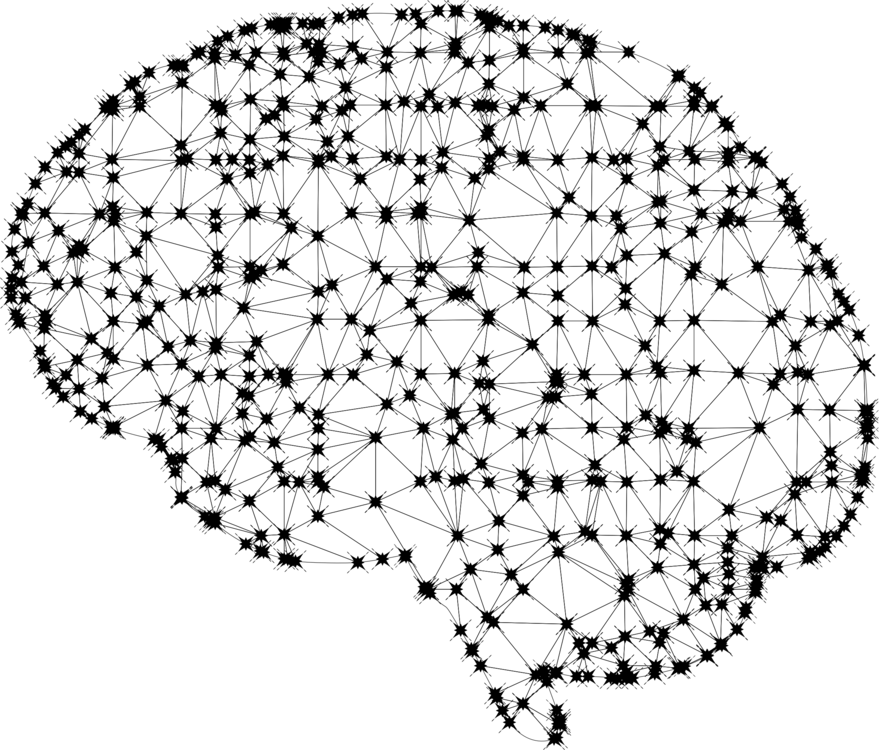
\includegraphics[scale=0.25]{../Images/brain.png}}{© Copyright trzcacak.rs}
	\caption{Artificial neural networks are inspired by neural networks in the brain.}
\end{figure}

% History
The use of the term \textit{machine learning} has exploded over the past years, and sometimes it even sounds like it is a new field. However, the truth is that many of the methods are relatively old, where for instance \textit{linear regression} was known in the early 19th-century when \citet{legendre_nouvelles_1805} and \citet{gauss_theoria_1809} independently developed the concepts of mean square error (MSE). Those methods have just recently been taken under the machine learning umbrella, which is one of the reasons why the term is used more frequently than before. Another essential contributor to the booming popularity is the dramatically improvement of a majority of the machine learning algorithms, most notably neural networks, as discussed in the introduction.

% What is Machine Learning?
Unlike traditional algorithms, machine learning algorithms are not explicitly told what to do, but they use optimization tools to minimize a \textit{cost function} and fit a model to data sets. As a consequence, we often do not know precisely what the algorithms do and why they behave as they do. Because of this behavior and the fact that artificial neural networks are inspired by the human brain, the processing is often called artificial intelligence. As a definition of the term machine learning, we use the definition by Stanford \cite{noauthor_machine_nodate}:

\begin{shadequote}{}
	Machine learning is the science of getting computers to act without being explicitly programmed.
\end{shadequote}

% Why Machine Learning?
In our search for a technique to solve quantum mechanical problems where less physical intuition is needed, machine learning appears as a natural tool. First, machine learning has proven an impressive ability of ... Second, ... With methods that do not require all the physical intuition about the system, we might be able to study complex systems that are out of reach with the current methods, like complex nuclear systems.

% How do we use Machine Learning?
We typically classify the machine learning methods as either supervised or unsupervised, based on the way we define the cost function. Supervised models are provided with \textit{targets}, which are outputs that the model should obtain with a certain input data set. We then define the cost function as the error between the output from the model and the targets, and the model is trained until it is able to reproduce the targets. On the other hand, unsupervised models are not provided with targets, and the cost function thus needs to be defined in another way. In our work, we aim to construct a robust method for the study of the ground state of complex systems, and as targets for those systems usually are unavailable, we will use unsupervised algorithms. More precisely, we will rely on restricted Boltzmann machines (RBM), where the cost function is defined as a system energy that we want to minimize. As there are many common concepts in supervised and unsupervised learning, we will in this chapter stick to supervised learning where we introduce essential concepts like artificial neurons, weights and optimization schemes. The Boltzmann machines, which are the models that we actually use in the work, are discussed in chapter \ref{chp:restricted}.

% The goal of supervised learning


As hinted above, in machine learning, we want to fit a model to a data set in the best possible way. In supervised learning, we have prior knowledge about what kind of results the model should give in some specific cases, which we can use to train our model. After training, we want the model to
\begin{enumerate}
	\item be able to reproduce the \textit{targets}, the prior known results.
	\item be able to fit future observations.
\end{enumerate}
In this chapter, we will examine how a model that satisfies both the requirements can be found, possible challenges and when the ansatz will break down. Subsequently, we will see that there is no guaranty that the second point is satisfied even when the first point is satisfied. First, the polynomial regression is presented to explain fundamental concepts of machine learning in an intuitive way, and thereafter we generalize the theory in form of linear regression. In the end, we go thorough neural networks which have many common features with the restricted Boltzmann machines discussed in the next chapter. 

\section{Polynomial regression}
The polynomial regression is perhaps the most intuitive example on supervised learning, as it can be used to solve problems everyone is familiar with. In general, polynomial regression finds the $p$'th degree polynomial, $f(x;\bs{c})=\sum_{i=0}^pc_ix^i$, that fits a set of points in the best possible way. In two dimensions, the data set consists of some $n$ number of $x$- and $y$-coordinates,
\begin{align*}
\bs{x}&=(x_1,x_2,\hdots,x_n)\\
\bs{y}&=(y_1,y_2,\hdots,y_n),
\end{align*}
henceforth denoted by $\mathcal{D}=\{\bs{x},\bs{y}\}$. The data set can for instance be fitted to a second-order polynomial,
\begin{equation}
f(x;a,b,c)=ax^2+bx+c,
\end{equation}
where the parameters $a$, $b$ and $c$ are our \textit{estimators}. The polynomial is now our model, and by evaluating it on all values in the $\bs{x}$-vector we obtain a set of $n$ equations
\begin{equation}
\mqty{
	\tilde{y}_1&=&ax_1^2&+&bx_1&+&c\\
	\tilde{y}_2&=&ax_2^2&+&bx_2&+&c\\
	\vdots&&\vdots&&\vdots&&\vdots\\
	\tilde{y}_n&=&ax_n^2&+&bx_n&+&c
}
\label{eq:lineareqs}
\end{equation}
where $\tilde{y}_i=f(x_i)$ is the output from the model with $x_i$ as the input. What we want to do is to determine the estimators $a$, $b$ and $c$ such that the mean squared error (MSE) of all these equations,
\begin{equation}
\min_{a,b,c}\frac{1}{n}\sum_{i=0}^{n-1}(y_i-f(x_i;a,b,c))^2,
\end{equation}
is minimized. The MSE is then defined as our cost function $\mathcal{C}(\bs{\theta})$ (also called the loss function), which is always the function that we try to minimize in machine learning. For our choice of model, the cost function reads
\begin{empheq}[box={\mybluebox[5pt]}]{equation}
\mathcal{C}(a,b,c)=\frac{1}{n}\sum_{i=0}^{n-1}\Big(y_i-(ax_i^2+bx_i+c)\Big)^2,
\end{empheq}
which can be minimized in several ways. Before we proceed to the minimization, we will introduce a more general notation, where the estimators are collected in a column vector 
\begin{equation}
\bs{\theta}\equiv(a,b,c)^T
\end{equation}
and the $x_i^j$'s are collected in a row vector
\begin{equation}
\bs{X}_i\equiv(x_i^2, x_i^1, x_i^0)=(x_i^2, x_i, 1).
\end{equation}
Using this, the cost function can be written as
\begin{equation}
\begin{aligned}
\mathcal{C}(\bs{\theta})&=\frac{1}{n}\sum_{i=0}^{n-1}\Big(y_i-\sum_{j=0}^2X_{ij}\theta_j\Big)^2\\
&=\frac{1}{n}\sum_{i=0}^{n-1}\Big(y_i-\bs{X}_i\bs{\theta}\Big)^2\\
&=\frac{1}{n}(\bs{y}-\bs{X}\bs{\theta})^T(\bs{y}-\bs{X}\bs{\theta})
\end{aligned}
\label{eq:polynomialcost}
\end{equation}
where we in the last step have collected all the vectors $\bs{X}_i$ in a matrix $\bs{X}=[\bs{X}_1,\bs{X}_2,\hdots,\bs{X}_n]$. As the minimum of the cost function with respect to an estimator $\theta_j$ is found when the derivative is zero, we need to solve
\begin{equation}
\begin{aligned}
\frac{\partial \mathcal{C}(\bs{\theta})}{\partial\theta_j} &=\frac{\partial}{\partial\theta_j}\bigg(\frac{1}{n}\sum_{i=0}^{n-1}\Big(y_i-\sum_{j=0}^2X_{ij}\theta_j\Big)^2\bigg)\\
&=\frac{2}{n}\sum_{i=0}^{n-1}X_{ij}\Big(y_i-\sum_{j=0}^2X_{ij}\theta_j\Big)=0.
\end{aligned}
\end{equation}
We can go further and write it on matrix-vector form as
\begin{equation}
\frac{\partial \mathcal{C}(\bs{\theta})}{\partial\bs{\theta}}=\frac{2}{n}\bs{X}^T(\bs{y}-\bs{X}\bs{\theta})=0
\end{equation}
where the differentiating is done element-wise, $\partial\mathcal{C(\bs{\theta})}/\partial\theta_j$. This is satisfied if and only if
\begin{equation}
\bs{\theta}=(\bs{X}^T\bs{X})^{-1}\bs{X}^T\bs{y}
\label{eq:polynomialestimators}
\end{equation}
which is the equation we seek to solve to find the best fitting polynomial. Before we proceed to the general case, let us take a quick look at an example.

\subsection{Example} \label{sec:example}
In this example, we will do the polynomial regression on an actual two-dimensional data set consisting of 10 points,
\begin{align}
\bs{x}&=(1,2,4,6,7,9,10,11,13,16)\notag\\
\bs{y}&=(15,30,50,60,65,63,60,55,40,0),
\label{eq:datapoints}
\end{align}
which is nothing else than a second-order polynomial with some noise. The data points are plotted in figure (\ref{fig:polynomials} a), and we want to fit a $p$'th degree polynomial to the points. The first thing we need to realize is that in order to validate our models, we cannot use all points for the training. There is no strict rule on how much of the data set that should be used for training and validation, but at least the training data set should be larger than the validation data set. For this particular problem, we decide to leave out $\{(1,15),(9,63),(10,60)\}$ from the training, which we later will use for validation.

Furthermore, we use equation \eqref{eq:polynomialestimators} to find the best fitting first-, second- and sixth-order polynomials, and obtain the functions presented in table \eqref{tab:example} with the respective training and prediction errors. The polynomials are also plotted in figure (\ref{fig:polynomials} b) together with the actual data points.

\begin{figure}[H]
	\centering
	\subfloat[Data set]{{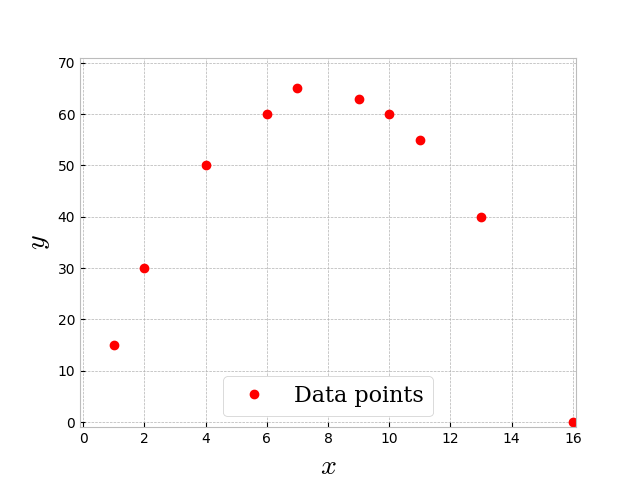
\includegraphics[width=8cm]{../Images/datapoints.png}}}
	\subfloat[Data set with fitted polynomials]{{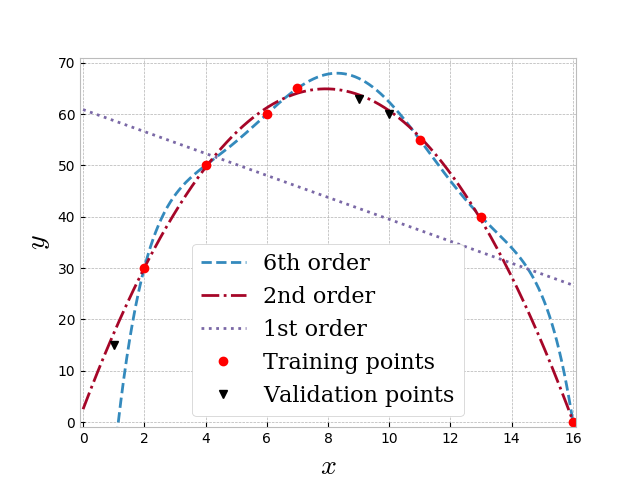
\includegraphics[width=8cm]{../Images/datacurve.png} }}
	\caption{Figure (a) presents the data points given in equation \eqref{eq:datapoints}, while the figure (b) illustrates how a first-, second- and sixth order polynomial can be fitted to the training set in the best possible way.}%
	\label{fig:polynomials}
\end{figure}

\begin{table}[H]
	\caption{Best fitting polynomials of first-, second- and sixth-order degree to the data set in equation \eqref{eq:datapoints}. $f(x)$ gives the actual form of the polynomial, the training error is the MSE of the training data set and the prediction error is the MSE of the validation data set.}
	\label{tab:example}
	\begin{tabularx}{\textwidth}{llR{6.5cm}R{3cm}R{3cm}} \hline\hline
		Order & \makecell{\\ \phantom{=}} & \multicolumn{1}{c}{$f(x)$} & Training error & Prediction error \\ \hline \\
		
		1st && $-2.14x+60.87$ & 327.22 & 927.87 \\
		2nd && $-x^2+15.74x + 2.51$ & 0.47 & 2.04 \\
		6th && $-0.001x^6+0.04x^5-0.90x^4+9.04x^3-47.52x^2+129.74x-98.67$ & 2.54E-11 & 187.53 \\ \hline\hline
	\end{tabularx}
\end{table}

What we immediately observe, is that the more complex model (higher degree polynomial), the lower the training error. The polynomial of sixth-order reproduces the points entirely. The first-order polynomial is quite bad, while the second-order polynomial is intermediate. However, what is most important is the prediction error as it shows the ability to reproduce data that is not prior known, and for that, we can see that the sixth order polynomial performs terribly. When a model can reproduce the training set very well but is not able to reproduce the training set, we say that it overfits the data set. This means that the model is too complicated for the purpose. On the other hand, we see that the first-order polynomial also has a significant prediction error, which means that it is not able to reproduce the validation set either. We say that it is under fitted, and we are in need of a more complex model.

Finally, we have the second-order polynomial, which is miles ahead of its competitors when it comes to the prediction error. It turns out that the second-order model has an appropriate complexity, which we could have guessed just by looking at the data points. The natural question now is \textit{"How do we find a correct model complexity?"}. The answer is that there no easy way of doing this, which is one reason why machine learning is difficult. The trail and error method is the standard approach, where one examines various complexities and calculate the prediction error for each model. To find the prediction error precisely, one typically uses $K$ cross-validation resampling, which evaluates $K$ different choices of validation set to make the most use of the data. More about resampling analysis can be found in section \eqref{sec:resampling}. A deeper understanding of the prediction error and how to reveal if a model overfits or under its will hopefully be gained in the next section, on bias-variance tradeoff. 

\section{Bias-variance tradeoff}
Up to this point, we have skipped some important terms in the statistics behind machine learning. First, we have the \textit{bias}, which describes the best our model could do if we had an infinite amount of training data. We also have the \textit{variance}, which is a measure of the fluctuations in the predictions. In figure (\ref{fig:bias_variance} a), an example of high variance low-bias and a low variance high bias models are presented. What we actually want is a low variance low-bias model, but this model is normally infeasible, and we need to find the optimal tradeoff between bias and variance. This is known as the bias-variance tradeoff. 

In figure (\ref{fig:bias_variance} b), the bias-variance tradeoff is illustrated as a function of the model complexity. We observe that the prediction error is large when the model complexity is too low, which corresponds to a low variance. This substantiates what we discussed in the example in section \ref{sec:example}, where we claimed that a too low model complexity under its data set. Therefore, a too low variance is associated with underfitting. On the other side of the plot, we can see that also a too complex model causes a large prediction error, which corresponds to a low bias. As discussed before, a too complex model overfits the model, which is associated with low bias. 

\begin{figure}
	\centering
	\subfloat[Illustration of bias and variance]{{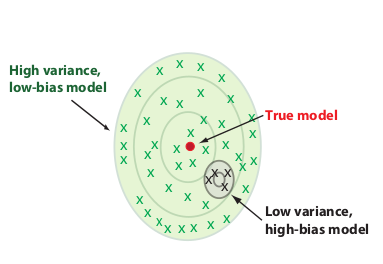
\includegraphics[width=8cm]{../Images/bias_variance.png}}}
	\subfloat[Bias-variance trade-off]{{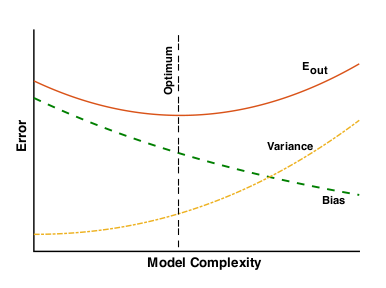
\includegraphics[width=8cm]{../Images/bias_variance_tradeoff.png} }}
	\caption{Examples of high variance, low-bias and low variance high-bias (a) and illustration of the bias-variance trade-off (b). Figures are taken from \citet{mehta_high-bias_2019}.}%
	\label{fig:bias_variance}
\end{figure}

To minimize the prediction error, we should therefore neither minimize the bias nor the variance. Instead, we should find the bias and variance which corresponds to the lowest error. To see how the error is distributed between the bias and variance, we can perform a so-called bias-variance decomposition. This is easiest if we assume that the true data is generated from a noisy model
\begin{equation}
y=f(x)+\epsilon
\end{equation}
where $\epsilon$ is normally distributed with mean zero and standard deviation $\sigma_{\epsilon}$. In that case, it can be shown that
\begin{equation}
\langle\langle(y_{\epsilon}-\tilde{y})^2\rangle\rangle_{\epsilon}=\underbrace{\sum_i(f(x_i)-\langle \tilde{y}\rangle)^2}_{\text{bias}^2}+\underbrace{\sum_i\langle(\tilde{y}-\langle \tilde{y}\rangle)^2\rangle}_{\text{variance}}+\underbrace{\sum_i\sigma_{\epsilon}^2}_{\text{noise}}
\end{equation}
where the expectation values are over the data set $\mathcal{D}$ if nothing else is specified. This decomposition is shown carefully by \citet{mehta_high-bias_2019}.

\section{Linear regression}
Polynomial regression, as already discussed, is an example on a linear regression method, and was meant as a motivation before we study linear regression in general. Instead of fitting a polynomial to a set of points, we can fit a general function in the form of
\begin{equation}
f(x_i)=\sum_{j=0}^pX_{ij}(x_i)\theta_j
\label{eq:targets}
\end{equation}
where we have $p+1$ estimators $\theta_j$. The matrix $\bs{X}$ is called the \textit{design matrix}, and in the case where $X_{ij}(x_i)=x_i^j$ corresponds to polynomial regression, but it can in principle be an arbitrary function of $x_i$. The cost function for \textit{the ordinary least square regression} (OLS) case is already found in equation \eqref{eq:costols}, and we can recall it as
\begin{empheq}[box={\mybluebox[5pt]}]{equation}
\mathcal{C}(\bs{\theta})=\sum_{i=1}^{n}\Big(y_i-\sum_{j=0}^pX_{ij}\theta_j\Big)^2,\qquad\qquad\qquad\text{OLS}
\end{empheq}
which is minimized when
\begin{equation}
\bs{\theta}=(\bs{X}^T\bs{X})^{-1}\bs{X}^T\bs{y}.
\label{eq:ols}
\end{equation}

To solve this equation, we need to find the inverse of the matrix $\bs{X}^T\bs{X}$, which is typically done by \textit{lower-upper} decomposition (LU) or \textit{singular values decomposition} (SVD). However, quite often, when we deal with large data sets, the matrix above is singular, which means that the determinant of the matrix is zero. In those cases, we cannot find the inverse, and LU decomposition does not work. Fortunately, SVD \textit{always} works, and in cases where the matrix is singular, it turns out to be a good idea to perform such decomposition.

\subsection{Singular value decomposition}
Singular value decomposition is a method which decomposes an $m\times n$ matrix $\bs{X}$ into a product of three matrices, written as
\begin{equation}
\bs{X}=\bs{U}\bs{\Sigma}\bs{V}^T
\end{equation}
where $\bs{U}$ is a unitary $m\times m$ matrix, $\bs{V}$ is a unitary $n\times n$ matrix and $\bs{\Sigma}$ is a diagonal $m\times n$ matrix. This might sounds like a bad idea, but especially for singular matrices this often makes life easier. The reason for this, is that only $\bs{\Sigma}$ is singular after the decomposition. For our case, we can thus write the matrix $\bs{X}^T\bs{X}$ as 
\begin{equation}
\bs{X}^T\bs{X}=\bs{V}\bs{\Sigma}^T\bs{\Sigma}\bs{V}^T=\bs{V}\bs{D}\bs{V}^T
\end{equation}
where we exploit that $\bs{U}^T\bs{U}=\mathbb{1}$ and $\bs{\Sigma}^T\bs{\Sigma}=\bs{D}$ by definition. Further we can multiply by $\bs{V}$ on the right-hand-side
\begin{equation}
(\bs{X}^T\bs{X})\bs{V}=\bs{V}\bs{D}
\end{equation}
to get rid of the $\bs{V}^T$. A similar exercise can be done on $\bs{X}\bs{X}^T$, and we will obtain
\begin{equation}
(\bs{X}\bs{X}^T)\bs{U}=\bs{U}\bs{D}.
\end{equation}
By using the former of the two expressions, one can show that
\begin{equation}
\bs{X}\bs{\theta}=\bs{U}\bs{U}^T\bs{y}
\end{equation}
which is solvable even when $\bs{X}^T\bs{X}$ is singular.

\subsection{Ridge regression}
So, how can we avoid non-singular values in our matrix $\bs{X}^T\bs{X}$? We can remove them by introducing a penalty $\lambda$ to ensure that all the diagonal values are non-zero, which can be accomplished by adding a small value to all diagonal elements. By doing this, all diagonal elements will get a non-zero value and the matrix is guaranteed to be non-singular. Still using the matrix-vector form, this can be written as 
\begin{equation}
\bs{\theta}=(\bs{X}^T\bs{X}+\lambda\bs{I})^{-1}\bs{X}^T\bs{y}
\label{eq:ridgetheta}
\end{equation}
where $\bs{I}$ is the identity matrix. The penalty $\lambda$ is also a \textit{hyper-parameter}, which is a parameter that is specified before the training begins, in contrast to the estimators which are determined throughout training. This method is called Ridge regression, and has a cost function given by 
\begin{empheq}[box={\mybluebox[5pt]}]{equation}
\mathcal{C}(\bs{\theta})=\sum_{i=1}^{n}\Big(y_i-\sum_{j=0}^pX_{ij}\theta_j\Big)^2+\lambda\sum_{j=1}^p|\theta_j|^2\qquad\text{Ridge}
\label{eq:ridge}
\end{empheq}
where we in principle just add the L2-norm of the estimator vector to the OLS cost function. The link between equation \eqref{eq:ridgetheta} and \eqref{eq:ridge} can be easiest found by going from the latter to the former, similarly to what we did for the polynomial regression in equations (\ref{eq:polynomialcost}-\ref{eq:polynomialestimators}).

\subsection{LASSO regression}
Finally, we introduce the \textit{least absolute shrinkage and selection operator} (LASSO) regression, which in the same way as Ridge regression is based on regularization. Instead of adding the L2-norm of the estimator matrix, we add the the L1-norm $|\theta_j|$, and the cost function expresses
\begin{empheq}[box={\mybluebox[5pt]}]{equation}
\mathcal{C}(\bs{\theta})=\sum_{i=1}^{n}\Big(y_i-\sum_{j=0}^pX_{ij}\theta_j\Big)^2+\lambda\sum_{j=1}^p|\theta_j|.\qquad\text{Lasso}
\end{empheq}
For LASSO regression, we cannot set $\partial\mathcal{C}(\bs{\theta})/\partial\theta_j=0$ and find a closed-form expression of $\bs{\theta}$, which means that we need to use an iterative optimization algorithm in order to obtain the optimal estimators. Such optimization methods are essential in non-linear problems such as deep neural networks and variational Monte-Carlo. They will therefore be familiar to the reader throughout this thesis. In section \ref{sec:optimizationalgorithms} we present various optimization methods, but for now on we will stick to one of the most basic methods, \textit{gradient descent}, which can be written as  
\begin{equation}
\theta_j^+=\theta_j-\eta \frac{\partial\mathcal{C}(\bs{\theta})}{\partial\theta_j},
\end{equation}
where $\theta_j^+$ is the updated version of $\theta_j$ and $\mathcal{C}(\bs{\theta})$ is an arbitrary cost function. Here we are introduced to a new hyper-parameter, $\eta$, known as the \textit{learning rate}, which controls how much the estimators should be changed for each iteration. It has to be specified carefully, where a too large $\eta$ will make the cost function diverge and a too small $\eta$ will make the training too slow. Typically, to choose an $\eta$ in the range 0.01-0.0001 is a good choice. For ordinary least squares, the vectorized parameter update can be written as
\begin{equation}
\bs{\theta}^+=\bs{\theta}-\eta\bs{X}^T(\bs{y}-\bs{X}\bs{\theta}).
\label{eq:olsupdate}
\end{equation}

\section{Logistic regression}
So far, we have discussed polynomial regression and linear regression, which consist of models giving continuous outputs. However, what do we do if we want discrete outputs, for example, in the form of classification? This is what logistic regression is all about, where the name comes from the logistic function (sigmoid function) which is used to fire or not fire the neurons. As for the linear regression, we also need a cost function in logistic regression, which we will motivate in the following.

Consider a system that can take two possible energies $\varepsilon_0$ and $\varepsilon_1$. From elementary statistical mechanics, we know that the probability of finding a system in a state of a certain energy is given by the Boltzmann distribution, such that
\begin{align}
P(y_i=0)&=\frac{\exp(-\varepsilon_0/k_BT)}{\exp(-\varepsilon_0/k_BT)+\exp(-\varepsilon_1/k_BT)}\\
&=\frac{1}{1+\exp(-(\varepsilon_1-\varepsilon_0)/k_BT)}
\end{align}
which is the \textit{sigmoid function}, in the most general given by
\begin{equation}
f(x)=\frac{1}{1+\exp(-x)}.
\end{equation}
The first denominator is known as the \textit{partition function},
\begin{equation}
Z=\sum_{i=0}^1\exp(-\varepsilon_i/k_BT)
\label{eq:partition}
\end{equation}
where $k_B$ is Boltzmann's constant and $T$ is the system temperature. The probability of finding the system in the second state is given by
\begin{align}
P(y_i=1)&=1-P(y_i=0)\\
&=\frac{1}{1+\exp(-(\varepsilon_0-\varepsilon_1)/k_BT)}.
\end{align}
Notice that the only thing we need is the energy difference between the two states rather than the energy itself. This is often the case in physics, where we for instance have no absolute potential energy. If we now assume that the energy difference can be written as a function of the coordinates that specify the state $i$ stored in the row vector $\bs{X}_i$, and a column vector with parameters, $\bs{w}$, known as the \textit{weights}, the difference can be written as
\begin{figure}
	\centering
	\begin{tikzpicture}
\node[functions] (center) {};
\node[below of=center,text width=4em] {Activation function};
\draw[thick] (0.5em,0.5em) -- (0,0.5em) -- (0,-0.5em) -- (-0.5em,-0.5em);
\draw (0em,0.75em) -- (0em,-0.75em);
\draw (0.75em,0em) -- (-0.75em,0em);
\node[right of=center] (right) {};
\path[draw,->] (center) -- (right);
\node[functions,left=3em of center] (left) {$\sum$};
\path[draw,->] (left) -- (center);
\node[weights,left=3em of left] (2) {$w_2$} -- (2) node[input,left=2em of 2] (l2) {$X_{i2}$};
\path[draw,->] (l2) -- (2);
\path[draw,->] (2) -- (left);
\node[below of=2] (dots) {$\vdots$} -- (dots) node[left=2em of dots] (ldots) {$\vdots$};
\node[weights,below of=dots] (n) {$w_n$} -- (n) node[input,left=2em of n] (ln) {$X_{in}$};
\path[draw,->] (ln) -- (n);
\path[draw,->] (n) -- (left);
\node[weights,above of=2] (1) {$w_1$} -- (1) node[input,left=2em of 1] (l1) {$X_{i1}$};
\path[draw,->] (l1) -- (1);
\path[draw,->] (1) -- (left);
\node[weights,above of=1] (0) {$b$} -- (0) node[input,left=2em of 0] (l0) {$B$};
\node[right of=0] {bias};
\path[draw,->] (l0) -- (0);
\path[draw,->] (0) -- (left);
\node[below of=ln] {inputs};
\node[below of=n] {weights}; 
\end{tikzpicture}
	\caption{Logistic regression model with $n$ inputs. Each input $X_{ij}$ is multiplied with a weight $w_j$, and the contributions from all units are summarized. The output is obtained after the sum is activated by an activation function.}
	\label{fig:single_perceptron}
\end{figure}
\begin{equation}
\varepsilon_1-\varepsilon_0=\bs{X}_i\bs{w}\equiv\tilde{y}_i,
\end{equation}
giving the conditional probability
\begin{equation}
P(\bs{X}_i,y_i|\bs{w})=\big(f(\bs{X}_i\bs{w})\big)^{y_i}\big(1-f(\bs{X}_i\bs{w})\big)^{1-y_i}.
\end{equation}
If we have a set of multiple states stored in a  $\mathcal{D}=\{(\bs{X}_i,y_i)\}$, the joint probability yields
\begin{equation}
P(\mathcal{D}|\bs{w})=\prod_{i=1}^n\big(f(\bs{X}_i\bs{w})\big)^{y_i}\big(1-f(\bs{X}_i\bs{w})\big)^{1-y_i}
\end{equation}
which is known as the \textit{likelihood}. The \textit{log-likelihood} function is simply the log of the likelihood, and is given by 
\begin{equation}
l(\bs{w})=\sum_{i=1}^n\bigg[y_i\log f(\bs{X}_i\bs{w})+(1-y_i)\log(1-f(\bs{X}_i\bs{w}))\bigg].
\end{equation}
As in linear regression, we want to find a cost function which we can minimize in order to fit the model to the data set. Since the log-likelihood function is at its maximum at the highest probability, a natural choice is to set the cost function to the negative log-likelihood function,
\begin{equation}
\mathcal{C}(\bs{w})=-l(\bs{w})=-\sum_{i=1}^n\Big[y_i\log f(\bs{X}_i\bs{w})+(1-y_i)\log(1-f(\bs{X}_i\bs{w}))\Big],
\end{equation}
which is the \textit{cross entropy}. To clarify things, we will try to illustrate how this works. In figure (\ref{fig:single_perceptron}), we have an input set $\bs{X}_i$ where each unit is multiplied with a parameter from $\bs{w}$ and summarized. This corresponds to the inner product $\bs{X}_i\bs{w}$. Further, the sum (or the inner product) is \textit{activated} by an \textit{activation function}, which we above have assumed to be the sigmoid function. The output is then given by
\begin{eqnarray}
a_i=f(\bs{X}_i\bs{w}).
\end{eqnarray}
where the bias node is included in the $\bs{X}_i$'s and the bias weights are included in the $\bs{w}$'s. The bias node is added in order to shift the activation function to the left or right, and works in the same way as a constant term in a function. 

The output from the activation is used further in the cost function to calculate the cost. As for LASSO regression, the cost function is then minimized in an iterative scheme, where for example the gradient descent method gives the weight update
\begin{empheq}[box={\mybluebox[5pt]}]{align}
\bs{w}^+= \bs{w} - \eta\bs{X}[\bs{y}-f(\bs{X}\bs{w})].
\end{empheq}
where $\bs{X}$ is a matrix containing all the column vectors $\bs{X}_i$. This expression is extremely similar, not to say identical to the estimator update for ordinary least square presented in equation \eqref{eq:olsupdate}. The difference is that we now denote the parameters by $\bs{w}$ instead of $\bs{\theta}$ to prepare for the neural networks, but they are basically the same thing. 

\section{Neural networks} \label{sec:neural_network}
Now we know enough to dive into the field of artificial neural networks. Neural networks can give either continuous or discrete outputs and are therefore, competitors to both linear and logistic regression. The great strength of neural networks is that one can add multiple \textit{layers}, which potentially makes the model extremely flexible. According to \textbf{the universal approximation theorem}, a neural network with only one hidden layer with a finite number of units can approximate any continuous function \cite{hornik_multilayer_1989}. However, often, multiple layers are used since those networks are in general known to be easier to train and work better for complex systems. Neural networks of more than one layer are called \textit{deep} networks, and as more layers are added, the network gets \textit{deeper}.

In figure \eqref{fig:neural_network}, we have illustrated a deep neural network with an unspecified number of layers and five hidden units in each layer. It has some similarities with the logistic regression model in figure \eqref{fig:single_perceptron}, but with multiple hidden layers and multiple outputs, this model is more complicated. We decided to drop the representation of the weights (apart from some selected labeled ones), but each line corresponds to a weight.

Without a hidden layer, we have seen that the update of weights is quite straight forward. For a neural network consisting of multiple layers, the question is: \textit{How do we update the weights when we do not know the values of the hidden units?} This will be explained in section \ref{sec:backward}, where backward propagation, the most popular technique for weight update in a neural network, is discussed. Before that, we will generalize the forward phase presented in logistic regression.

\begin{figure}
	\centering
	\begin{tikzpicture}

% Define outputs
\node[] (center) {};
\node[input, above=0.3em of center] (y1) {$y_1$};
\node[input, below=0.3em of center] (y2) {$y_2$};

% Draw lines from output nodes
\node[right of=y1] (righty1) {};
\node[right of=y2] (righty2) {};
\path[draw,->] (y1) -- (righty1);
\path[draw,->] (y2) -- (righty2);

% Hidden nodes L
\node[input,left=5em of center] (aL3) {$a_3^{(L)}$};
\node[input,above of=aL3] (aL2) {$a_2^{(L)}$};
\node[input,above of=aL2] (aL1) {$a_1^{(L)}$};
\node[input,below of=aL3] (aL4) {$a_4^{(L)}$};
\node[input,below of=aL4] (aL5) {$a_5^{(L)}$};
\node[input,above of=aL1] (bL) {$B_L$};

% Hidden nodes 1
\node[input,left=25em of center] (a13) {$a_3^{(1)}$};
\node[input,above of=a13] (a12) {$a_2^{(1)}$};
\node[input,above of=a12] (a11) {$a_1^{(1)}$};
\node[input,below of=a13] (a14) {$a_4^{(1)}$};
\node[input,below of=a14] (a15) {$a_5^{(1)}$};
\node[input,above of=a11] (b1) {$B_1$};

% Hidden nodes l
\node[input,left=15em of center] (al3) {$a_3^{(l)}$};
\node[input,above of=al3] (al2) {$a_2^{(l)}$};
\node[input,above of=al2] (al1) {$a_1^{(l)}$};
\node[input,below of=al3] (al4) {$a_4^{(l)}$};
\node[input,below of=al4] (al5) {$a_5^{(l)}$};
\node[input,above of=al1] (bl) {$B_l$};

% Draw lines from hidden nodes
\path[draw,->] (aL1) -- (y1);
\path[draw,->] (aL2) -- (y1);
\path[draw,->] (aL3) -- (y1);
\path[draw,->] (aL4) -- (y1);
\path[draw,->] (aL5) -- (y1);
\path[draw,->] (bL) -- (y1);

\path[draw,->] (aL1) -- (y2);
\path[draw,->] (aL2) -- (y2);
\path[draw,->] (aL3) -- (y2);
\path[draw,->] (aL4) -- (y2);
\path[draw,->] (aL5) -- (y2) node[midway,below] {$w_{52}^{(L+1)}$};
\path[draw,->] (bL) -- (y2);

% Define place left of left
\node[input,left=5em of a13] (x2) {$x_2$};
\node[input,above of=x2] (x1) {$x_1$};
\node[input,below of=x2] (x3) {$x_3$};
\node[input,above of=x1] (b0) {$B_0$};

% Draw lines from input nodes
\path[draw,->] (x1) -- (a11);
\path[draw,->] (x1) -- (a12);
\path[draw,->] (x1) -- (a13);
\path[draw,->] (x1) -- (a14);
\path[draw,->] (x1) -- (a15);

\path[draw,->] (x2) -- (a11);
\path[draw,->] (x2) -- (a12);
\path[draw,->] (x2) -- (a13);
\path[draw,->] (x2) -- (a14);
\path[draw,->] (x2) -- (a15);

\path[draw,->] (x3) -- (a11);
\path[draw,->] (x3) -- (a12);
\path[draw,->] (x3) -- (a13);
\path[draw,->] (x3) -- (a14);
\path[draw,->] (x3) -- (a15) node[midway,below] {$w_{35}^{(1)}$};

\path[draw,->] (b0) -- (a11);
\path[draw,->] (b0) -- (a12);
\path[draw,->] (b0) -- (a13);
\path[draw,->] (b0) -- (a14);
\path[draw,->] (b0) -- (a15);

% Draw lines from first hidden layer
\path[draw,dashed,->] (a11) -- (al1);
\path[draw,dashed,->] (a11) -- (al2);
\path[draw,dashed,->] (a11) -- (al3);
\path[draw,dashed,->] (a11) -- (al4);
\path[draw,dashed,->] (a11) -- (al5);

\path[draw,dashed,->] (a12) -- (al1);
\path[draw,dashed,->] (a12) -- (al2);
\path[draw,dashed,->] (a12) -- (al3);
\path[draw,dashed,->] (a12) -- (al4);
\path[draw,dashed,->] (a12) -- (al5);

\path[draw,dashed,->] (a13) -- (al1);
\path[draw,dashed,->] (a13) -- (al2);
\path[draw,dashed,->] (a13) -- (al3);
\path[draw,dashed,->] (a13) -- (al4);
\path[draw,dashed,->] (a13) -- (al5);

\path[draw,dashed,->] (a14) -- (al1);
\path[draw,dashed,->] (a14) -- (al2);
\path[draw,dashed,->] (a14) -- (al3);
\path[draw,dashed,->] (a14) -- (al4);
\path[draw,dashed,->] (a14) -- (al5);

\path[draw,dashed,->] (a15) -- (al1);
\path[draw,dashed,->] (a15) -- (al2);
\path[draw,dashed,->] (a15) -- (al3);
\path[draw,dashed,->] (a15) -- (al4);
\path[draw,dashed,->] (a15) -- (al5) node[midway,below] {$w_{55}^{(l)}$};

\path[draw,dashed,->] (b1) -- (al1);
\path[draw,dashed,->] (b1) -- (al2);
\path[draw,dashed,->] (b1) -- (al3);
\path[draw,dashed,->] (b1) -- (al4);
\path[draw,dashed,->] (b1) -- (al5);

% Draw lines to last hidden layer
\path[draw,dashed,->] (al1) -- (aL1);
\path[draw,dashed,->] (al1) -- (aL2);
\path[draw,dashed,->] (al1) -- (aL3);
\path[draw,dashed,->] (al1) -- (aL4);
\path[draw,dashed,->] (al1) -- (aL5);

\path[draw,dashed,->] (al2) -- (aL1);
\path[draw,dashed,->] (al2) -- (aL2);
\path[draw,dashed,->] (al2) -- (aL3);
\path[draw,dashed,->] (al2) -- (aL4);
\path[draw,dashed,->] (al2) -- (aL5);

\path[draw,dashed,->] (al3) -- (aL1);
\path[draw,dashed,->] (al3) -- (aL2);
\path[draw,dashed,->] (al3) -- (aL3);
\path[draw,dashed,->] (al3) -- (aL4);
\path[draw,dashed,->] (al3) -- (aL5);

\path[draw,dashed,->] (al4) -- (aL1);
\path[draw,dashed,->] (al4) -- (aL2);
\path[draw,dashed,->] (al4) -- (aL3);
\path[draw,dashed,->] (al4) -- (aL4);
\path[draw,dashed,->] (al4) -- (aL5);

\path[draw,dashed,->] (al5) -- (aL1);
\path[draw,dashed,->] (al5) -- (aL2);
\path[draw,dashed,->] (al5) -- (aL3);
\path[draw,dashed,->] (al5) -- (aL4);
\path[draw,dashed,->] (al5) -- (aL5) node[midway,below] {$w_{55}^{(L)}$};

\path[draw,dashed,->] (bl) -- (aL1);
\path[draw,dashed,->] (bl) -- (aL2);
\path[draw,dashed,->] (bl) -- (aL3);
\path[draw,dashed,->] (bl) -- (aL4);
\path[draw,dashed,->] (bl) -- (aL5);

% Draw lines towards input nodes
\node[left of=x1] (leftx1) {};
\node[left of=x2] (leftx2) {};
\node[left of=x3] (leftx3) {};
\path[draw,->] (leftx1) -- (x1);
\path[draw,->] (leftx2) -- (x2);
\path[draw,->] (leftx3) -- (x3); 

% Add some text
\node[below=6.1em of x2] {input};
\node[below=6em of a13] {hidden 1};
\node[below=6em of al3] {hidden l};
\node[below=6em of aL3] {hidden L};
\node[below=6.8em of center] {output};
\end{tikzpicture}
	\caption{Neural network with 3 input units, $L$ hidden layers with 5 hidden units each and two outputs. $B_0$, $B_1$, $B_l$ and $B_L$ are bias units for their respective layers, and the dashed lines indicate that it might be more layers between the two layers. We have labeled a few of the lines to relate them to the weights. }
	\label{fig:neural_network}
\end{figure}

\subsection{Forward phase}
In the previous section, we saw how the output is found for a single perceptron. For a neural network, the net output to the first layer is similar, and given by
\begin{equation*}
z_j^{(1)}=\sum_{i=1}^{N_0}x_iw_{ij}^{(1)}=\bs{X}\bs{w}_j^{(1)}
\end{equation*}
where $N_0$ is the number of units in layer 0 (the input layer), $\bs{X}$ is the input vector which is assumed to be a row vector and $\bs{w}_j^{(1)}$ is the $i$'th column of the $\bs{w}$-matrix associated with the first layer. We have again assumed that the bias node is included in $\bs{X}$ and the first set of bias weights are included in $\bs{w}^{(1)}$. The same applies for the other layers as well. If we let the activation function, $f(x)$, act on the net output, we get the real output given by
\begin{equation*}
a_j^{(1)}=f(z_j^{(1)})=f\Big(\sum_{i=1}^{N_0}x_iw_{ij}^{(1)}\Big).
\end{equation*}
This is then again the input to the next layer with $N_1$ units, so the output from the second layer is simply
\begin{equation*}
a_j^{(2)}=f\Big(\sum_{i=1}^{N_1}a_i^{(1)}w_{ij}^{(2)}\Big).
\end{equation*}
For a neural network of multiple layers, the same procedure applies for all the layers and we can find a general formula for the output at a layer $l$. The net output to a node $z_j^{(l)}$ in layer $l$ can be found to be
\begin{empheq}[box={\mybluebox[5pt]}]{equation}
z_j^{(l)}=\sum_{i=1}^{N_{l-1}}a_i^{(l-1)}w_{ij}^{(l)}
\label{eq:netoutput}
\end{empheq}
where layer $l-1$ has $N_{l-1}$ units and we need to be aware that $a_j^{(0)}=x_j$. After activation, the output is obviously found to be
\begin{empheq}[box={\mybluebox[5pt]}]{equation}
a_j^{(l)}=f\Big(\sum_{i=1}^{N_{l-1}}a_i^{(l-1)}w_{ij}^{(l)}\Big)
\label{eq:output}
\end{empheq}
which is the only formula needed for the forward phase. In practice, the operation is always implemented in a vectorized fashion, reading $\bs{a}^{(l)}=f(\bs{a}^{(l-1)}\bs{w}^{(l)})$. The activation function $f(x)$ is not explicitly defined, because it is often expedient having the chance to experiment with multiple activation functions. 

\subsection{Activation function}
The task of the activation function is to define the output from a unit given an input. There are multiple reasons to do this, where the most important include filter the intensity of the output and make the output non-linear. Without an activation function, all of our layers would simply stack one affine transformation after another, resulting in a composition of transformations equal to such transformation. In other words, the deep networks would have lost their clout without the activation functions. 

Yet, we have only discussed the sigmoid activation function, but there plenty of other activation functions available. The sigmoid function has lost its popularity, and is today superseded by the more advanced functions based on \textit{rectified linear units} (ReLU). Some popular choices are the \textit{leaky} ReLU and \textit{exponential linear units} (ELU), which are linear for positive numbers. The pure linear activation function is still widely used, especially on the output layer. In figure (\ref{fig:activation_functions}), standard RELU, leaky RELU and ELU are plotted along with the sigmoid function.

\begin{figure}
	\centering
	\subfloat{{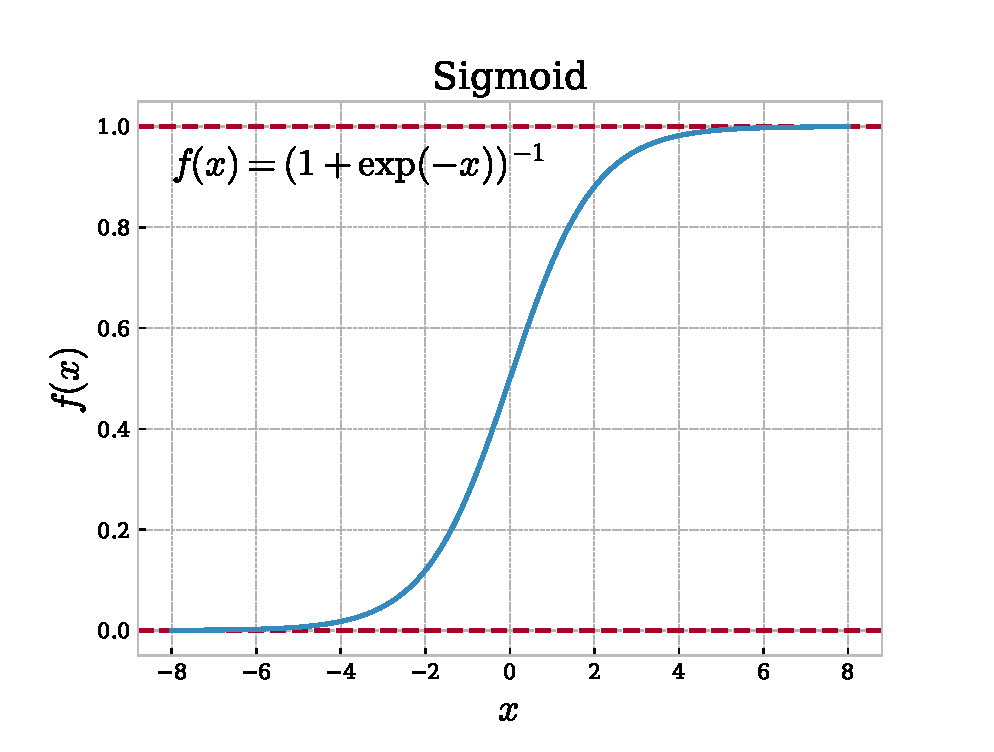
\includegraphics[width=7cm]{../Images/sigmoid.eps}}}
	\subfloat{{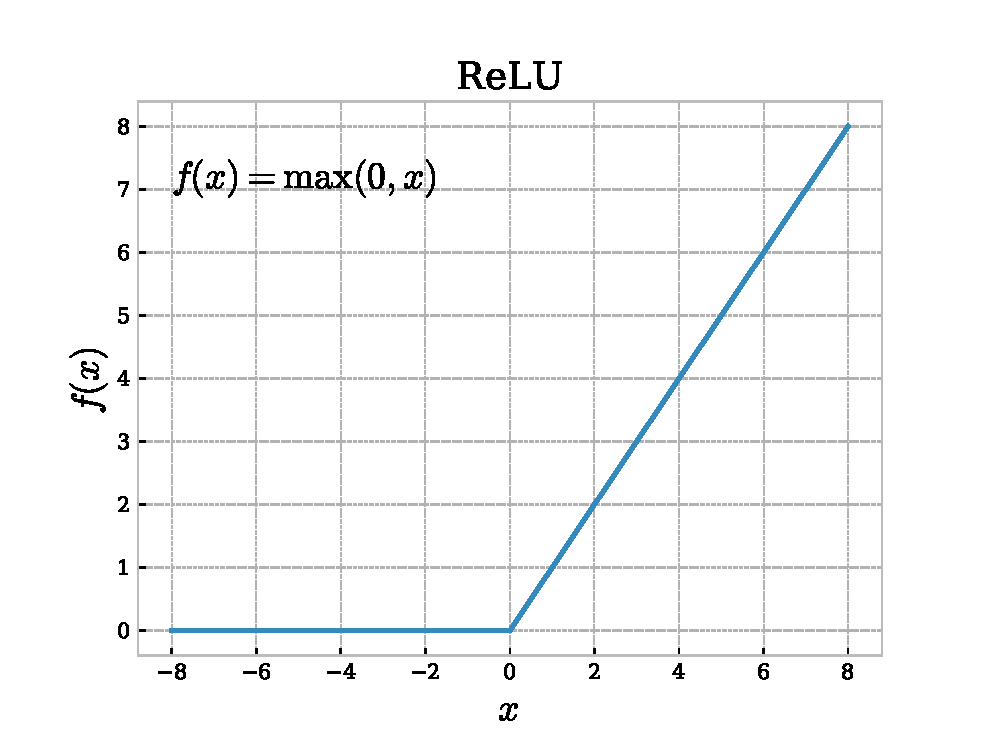
\includegraphics[width=7cm]{../Images/ReLU.eps}}}\\
	
	\subfloat{{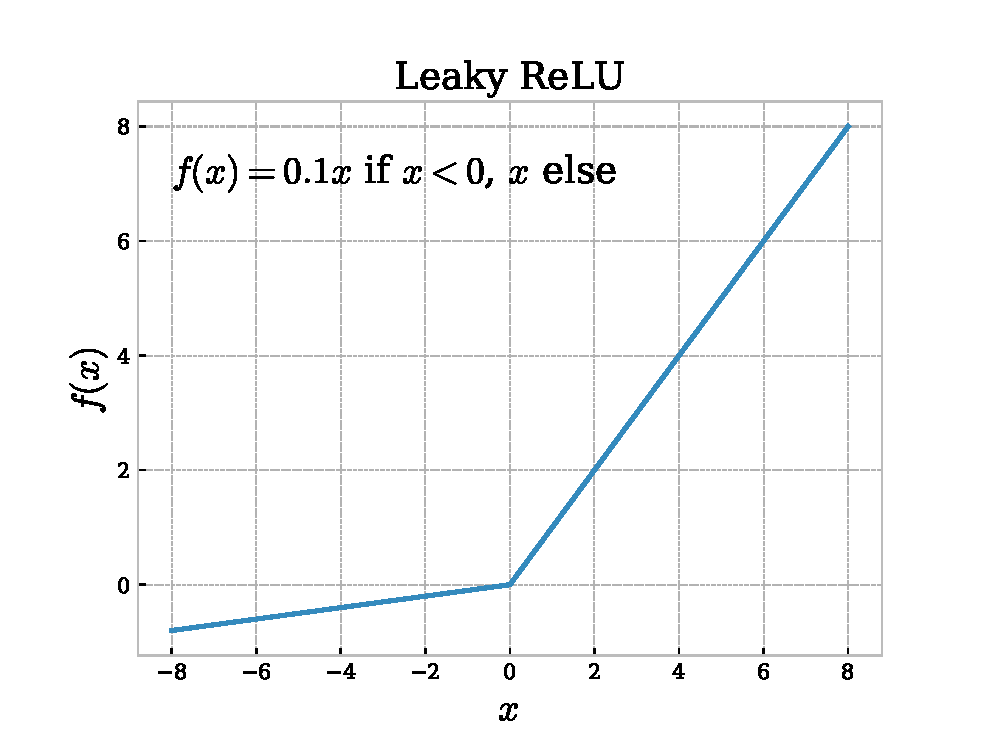
\includegraphics[width=7cm]{../Images/LeakyReLU.eps}}}
	\subfloat{{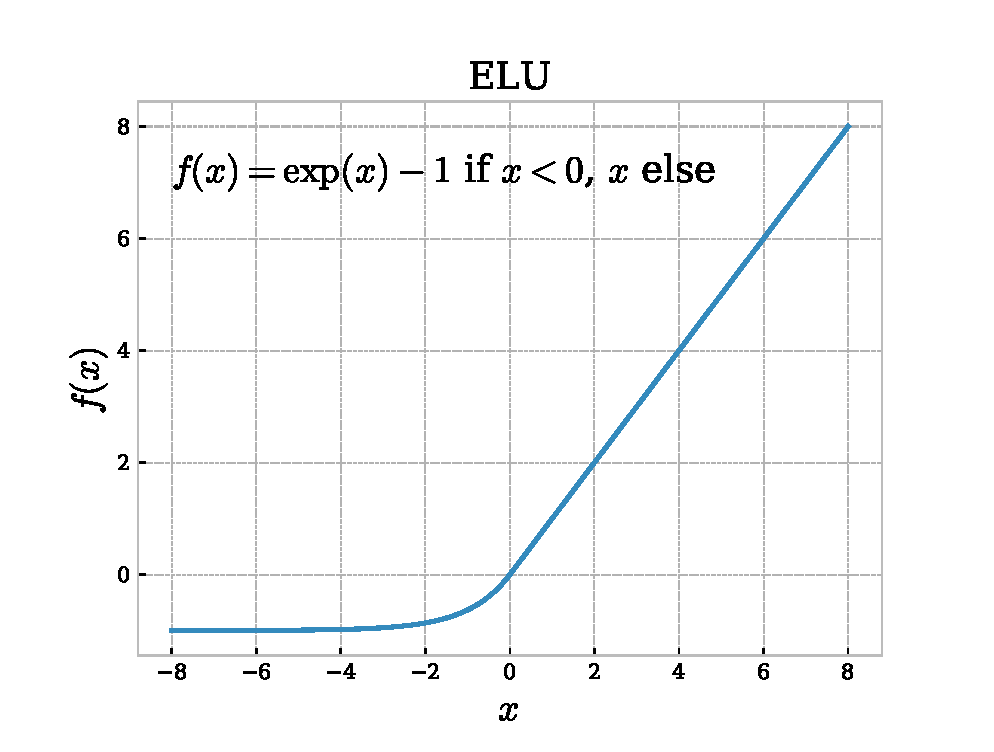
\includegraphics[width=7cm]{../Images/ELU.eps}}}
	\caption{Some well-known activation functions. The sigmoid function stands out from the others since it maps between 0 and 1, and it is not linear for positive numbers.}%
	\label{fig:activation_functions}%
\end{figure}


\subsection{Backward propagation} \label{sec:backward}
Backward propagation is the most robust technique for updating the weights in a neural network and is again based on the weight update presented for linear and logistic regression. The algorithm for this was presented in 1986, which made the deep neural networks able to solve relatively complicated problems for the first time \cite{rumelhart_learning_1986}. To update the weights, one starts with the outputs and updates the weights layer-wise until one gets to the inputs, hence the backward propagation name. 

As observed above, a node is dependent on all the units in the previous layers, and so are the weights. This means that the units are dependent on a large number of parameters, which makes the training scheme quite complex. Nevertheless, it is possible to generalize this to express the updating formulas on a relatively simple form, like the forward phase. From the linear and logistic regression, we know that we need the derivative of the cost function in order to implement the weight update regime. Again, we define the cost function as the mean square error,
\begin{equation}
\mathcal{C}(\bs{w})=\frac{1}{2}\sum_{i=1}^{N_L}(y_i-a_i^{(L)})^2
\end{equation}
where we have $L+1$ layers ($L$ is the last layer) and $N_L$ output units. The derivative of this with respect to one of the weights between the $L-1$'th and $L$'th layer can be written as a sum using the chain rule
\begin{equation}
\frac{\partial\mathcal{C}(\bs{w})}{\partial w_{jk}^{(L)}}=\frac{\partial\mathcal{C}(\bs{w})}{\partial a_j^{(L)}}\frac{\partial a_j^{(L)}}{\partial z_j^{(L)}}\frac{\partial z_j^{(L)}}{\partial w_{jk}^{(L)}}.
\end{equation}
where $z_j^{(L)}$ and $a_j^{(L)}$ are found from equations \eqref{eq:netoutput} and \eqref{eq:output} respectively. If we start with the first factor, it can easily be obtained as
\begin{equation}
\frac{\partial\mathcal{C}(\bs{w})}{\partial a_j^{(L)}}=-(y_j-a_j^{(L)})
\end{equation}
using the definition of the cost function. The second factor is the derivative of the activation function with respect to its argument, and is for the sigmoid function given by
\begin{equation}
\frac{\partial a_j^{(L)}}{\partial z_j^{(L)}}=a_j^{(L)}(1-a_j^{(L)}).
\end{equation}
Finally, the last factor is found from equation \eqref{eq:netoutput}, and we obtain
\begin{equation}
\frac{\partial z_j^{(L)}}{\partial w_{jk}^{(L)}}=a_k^{(L-1)}.
\end{equation}
Collecting all the factors, the update of the last set of weights can be found by
\begin{equation}
\frac{\partial\mathcal{C}(\bs{w})}{\partial w_{jk}^{(L)}}=-(y_j-a_j^{(L)})a_j^{(L)}(1-a_j^{(L)})a_k^{(L-1)}.
\end{equation}
when the sigmoid function is used in the activation. In the next step, we can define
\begin{equation}
\delta_j^{(L)}=-a_j^{(L)}(1-a_j^{(L)})(y_j-a_j^{(L)})=f'(a_j^{(L)})\frac{\partial \mathcal{C}(\bs{w})}{\partial a_j^{(L)}}=\frac{\partial \mathcal{C}(\bs{w})}{\partial z_j^{(L)}}
\end{equation}
such that the weight update can be expressed on a neater form
\begin{equation}
\frac{\partial\mathcal{C}(\bs{w})}{\partial w_{jk}^{(L)}}=\delta_j^{(L)}a_k^{(L-1)}.
\end{equation}

For a general layer $l$, the derivative of the cost function with respect to a weight $w_{jk}^{(l)}$ is similar, and given by
\begin{empheq}[box={\mybluebox[5pt]}]{equation}
\frac{\partial\mathcal{C}(\bs{w})}{\partial w_{jk}^{(l)}}=\delta_j^{(l)}a_k^{(l-1)}.
\end{empheq}
Our goal is to find the general relation between layer $l$ and $l+1$, and therefore we use the chain rule and sum over all the net outputs in layer $l+1$,
\begin{equation}
\delta_j^{(l)}=\frac{\partial \mathcal{C}(\bs{w})}{\partial z_j^{(l)}}=\sum_k\frac{\partial\mathcal{C}(\bs{w})}{\partial z_k^{(l+1)}}\frac{\partial z_k^{(l+1)}}{\partial z_j^{(l)}}.
\end{equation}
We now recognize that the first factor in the sum is just $\delta_k^{(l+1)}$ and the last factor can be found from equation \eqref{eq:netoutput}. We obtain the final expression, 
\begin{empheq}[box={\mybluebox[5pt]}]{equation}
\delta_j^{(l)}=\sum_k\delta_k^{(l+1)}w_{kj}^{(l+1)}f'(z_j^{(l)})
\end{empheq}
where we use the expression of $\delta_j^{(L)}$ as our initial condition. As for several of the methods discussed above, a solution of the weight update does not exist in closed form and we need to rely on iterative optimization methods. Using gradient descent, a new weight $w_{ij}^{(l)+}$ is found from
\begin{equation}
w_{ij}^{(l)+}=w_{ij}^{(l)}-\eta\frac{\partial\mathcal{C}(\bs{w})}{\partial w_{ij}^{(l)}},
\end{equation}
where other optimization methods will be discussed in the following section.

\section{Optimization algorithms} \label{sec:optimizationalgorithms}
We have above discussed the gradient descent optimization algorithm, which is among the most basic optimization methods available. That method is based on the gradient, which is the slope of the cost function. However, many other methods are also in need of the Hessian matrix, which gives the curvature of the cost function. We will barely scratch the surface of this field, limiting us to the gradient methods. 

To have the method fresh in mind, we will start with reintroducing the gradient descent method before we move on to its stochastic brother. We will then take a look at how momentum can be added, and finally, we examine the stochastic and momentum-based ADAM optimizer. Given a cost function $\mathcal{C}(\bs{\theta})$, the gradient with respect to a parameter $\theta$ can be found from
\begin{equation}
\nabla_{\theta} \mathcal{C}(\bs{\theta})\equiv\frac{\partial \mathcal{C}(\bs{\theta})}{\partial \bs{\theta}},
\end{equation}
where we henceforth use the short-hand notation with $\nabla_{\theta}$ representing the multi-dimensional derivative $\partial/\partial\bs{\theta}$. Differentiating with respect to the vector implies that the operation shall be done element-wise.

\subsection{Gradient descent} \label{sec:gd}
Perhaps the simplest and most intuitive method for finding the minimum is the gradient descent method, which reads
\begin{empheq}[box={\mybluebox[5pt]}]{align}
\label{eq:GD}
\bs{\theta}_t=\bs{\theta}_{t-1} - \eta\nabla_{\theta} \mathcal{C}(\bs{\theta}_{t-1})
\end{empheq}
where $\bs{\theta}_t$ is the parameter vector at time step (iteration) $t$ and $\eta$ is the learning rate. $\nabla_{\theta} \mathcal{C}(\bs{\theta}_{t-1})$ is the gradient of the cost function with respect to all the parameters $\theta$ at time $t-1$. 

The idea is to find the direction where the cost function $\mathcal{C}(\bs{\theta})$ has the steepest slope, and move in the direction which minimizes the cost function. For every time step, the cost function is thus minimized, and when the gradient approaches zero, the minimum is found. A possible, but basic, stop criterion is
\begin{equation}
\nabla_{\theta} \mathcal{C}(\bs{\theta}_t)<\varepsilon.
\end{equation}
where $\varepsilon$ is a tolerance. More robust methods are based on comparing the value of the cost function for several past iterations. In cases where the cost function is not strictly decreasing, we will have both local and global minima. Often, it is hard to say whether we are stuck in a local or global minimum, and this is where the stochasticity enters the game.

\subsection{Stochastic gradient descent}\label{sec:sgd}
Stochastic gradient descent is closely related to the gradient descent method, but the method uses randomly selected batches to evaluate the gradients, hence the stochasticity. By introducing this randomness, the parameters will not always be updated in order to minimize the energy, which makes us less likely to be stuck in a local minimum.

In practice, one splits the data set in $n$ batches, and select one of them to be used in the parameter update. Our hope is that this batch is representative of the entire data set, such that the new parameters provide a lower cost function. If that is the case, we have reduced the cost of an iteration significantly, since we only need to care about a batch. We are not guaranteed that updating the parameters with respect to a batch gives a lower cost function, and when it is not, we need to run more batches in order to minimize the cost function. Since each iteration is faster than for standard gradient descent, this is acceptable. As long as the batch is slightly representative of the entire data set, the cost function will be minimized in the end. After each batch in the data set has had an opportunity to update the internal parameters, we say that we have gone through an \textit{epoch}. Mathematically, the method can be expressed as 
\begin{empheq}[box={\mybluebox[5pt]}]{align}
\label{eq:SGD}
\bs{\theta}_t=\bs{\theta}_{t-1} - \eta\nabla_{\theta} \mathcal{C}_i(\bs{\theta}_{t-1})
\end{empheq}
where we use the $i$'th batch in the parameter update. Standard gradient descent is just a special case of this, where we only have one batch ($i$ includes the whole data set). If we still get stuck in local minima after adding the stochasticity, it might be a good idea to add momentum as well.

\subsection{Adding momentum} \label{sec:momentum}
If we now recall what we learned in an introductory mechanics course, we might remember that momentum is a quantity that maintains the motion of a body. Imagine a ball that rolls down a steep hill, but then there is a local minimum that it needs to escape to keep rolling. If it has enough momentum, it will be able to escape.

The same idea lies behind the momentum used in optimization algorithms; the momentum will try to maintain the motion towards the global minimum, which makes the system less likely to be stuck in a local minimum. Momentum can be added to most optimization algorithms, also gradient descent and stochastic gradient descent. The way we do it is to save the direction we were moving during the previous iteration, and use it as a contribution to the next gradient update. A typical implementation of the first-order momentum applied on gradient descent looks like
\begin{empheq}[box={\mybluebox[5pt]}]{equation}
\begin{aligned}
\bs{m}_t &= \gamma\bs{m}_{t-1} + \eta\nabla_{\theta} \mathcal{C}_i(\bs{\theta}_{t-1})\\
\bs{\theta}_t&=\bs{\theta}_{t-1}-\bs{m}_t
\end{aligned}
\end{empheq}
where $\gamma$ is the momentum parameter, which is just another hyper-parameter usually initialized to a small number. $\bs{m}_t$ is the momentum vector and can be initialized as the zero vector, corresponding to no initial momentum.

\IncMargin{1em}
\begin{algorithm}
	\SetAlgoLined
	\Parameter{$\eta$: Learning rate}
	\Parameter{$\gamma$: Momentum parameter}
	\Parameter{$\lambda$: Monotonic decay rate}
	\Require{$\mathcal{C}(\bs{\theta})$: Cost function}
	\Data{$\bs{\theta}_0$: Initial parameters}
	
	$\bs{m}_0\leftarrow 0$ (Initialize momentum vector)\;
	$t\leftarrow 0$ (Initialize time step)\;
	\While{$\bs{\theta}_t$ not converged}{
		$t\leftarrow t+1$ (Increase time for each iteration)\;
		$\bs{g}_t\leftarrow \nabla_{\theta}\mathcal{C}_t(\bs{\theta}_{t-1})$ (Get gradients from a given batch at time $t$)\;
		$\bs{m}_t\leftarrow \gamma\bs{m}_{t-1}+\eta\cdot\bs{g}_t$ (Update first momentum estimate)\;
		$\bs{\theta}_t=\bs{\theta}_{t-1}-\eta\cdot\bs{m}_t/\lambda^t$ (Update parameters with monotonic, adaptive step)\;
	}
	\KwResult{Converged parameters $\bs{\theta}_t$.}
	\caption{Adaptive stochastic gradient descent with momentum. See sections (\ref{sec:sgd}-\ref{sec:momentum}) for details. Robust default settings for the hyper-parameters are $\eta=0.001$, $\gamma=0.01$ and $\lambda=0.1$. All the operations are element-wise.}
	\label{alg:asgd}
\end{algorithm}\DecMargin{1em}

The optimization algorithm can be modified further in unlimited ways. A common improvement is to add higher-order momentum; another is to make the learning-rate adaptive. We have implemented the most basic version of this, with monotonic adaptivity. Many algorithms, such as the conjugate gradient method, also make use of the Hessian as discussed in the introductory word to this section, but that is another level of complexity. We will end this section by setting up the algorithm of a stochastic gradient descent optimization with momentum and monotonic adaptivity. The algorithm is found in algorithm \ref{alg:asgd}.

\subsection{ADAM} \label{sec:adam}
ADAM is a first-order stochastic optimization method which is widely used in machine learning. It was discovered by \citet{kingma_adam:_2014}, and published in a 2014 paper. The article has already more than 25000 citations! So what makes this method so popular? 

The main reason why it is widely used, is obviously that it provides good performance. The fact that it only requires the gradient makes it efficient, and the way the momentum is implemented still makes it capable of handle a large number of parameters. The optimization algorithm can be expressed as a set of equations
\begin{empheq}[box={\mybluebox[5pt]}]{equation}
\begin{aligned}
\bs{g}_t&=\nabla_{\theta} \mathcal{C}_t(\bs{\theta}_{t-1})\\
\bs{m}_t&=\gamma_1\bs{m}_{t-1}+(1-\gamma_1)\bs{g}_t\\
\bs{v}_t&=\gamma_2\bs{v}_{t-1}+(1-\gamma_2)\bs{g}_t^2\\
\hat{\bs{m}}_t&=\bs{m}_t/(1-\gamma_1^t)\\
\hat{\bs{v}}_t&=\bs{v}_t/(1-\gamma_2^t)\\
\bs{\theta}_t&=\bs{\theta}_{t-1}-\eta\hat{\bs{m}}_t/(\sqrt{\hat{\bs{v}}_t}+\bs{\varepsilon})
\end{aligned}
\end{empheq}
where $\bs{m}_t$ is the biased first momentum estimate of the parameter vector $\bs{\theta}$ and $\bs{v}_t$ is the biased second raw moment estimate. The momentum parameters need to be in the range $\gamma_1,\gamma_2\in[0,1)$, and are often set to values close to 1. This makes the optimization adaptive, as the time goes the factors $1-\gamma_1^t$ and $1-\gamma_2^t$ approach 1 from below. $\eta$ is the learning rate, and should be a small number. Finally, the parameter $\varepsilon$ is added to avoid division by zero. We can set up the algorithm in a way similar to the adaptive stochastic gradient descent algorithm presented above, which gives the algorithm \ref{alg:adam}.

\IncMargin{1em}
\begin{algorithm}
	\SetAlgoLined
	\Parameter{$\eta$: Learning rate}
	\Parameter{$\gamma_1,\gamma_2\in [0,1)$: Momentum parameters}
	\Parameter{$\varepsilon$: Division parameter}
	\Require{$\mathcal{C}(\bs{\theta})$: Cost function}
	\Data{$\bs{\theta}_0$: Initial parameters}
	
	$\bs{m}_0\leftarrow 0$ (Initialize 1$^{\text{st}}$ momentum vector)\;
	$\bs{v}_0\leftarrow 0$ (Initialize 2$^{\text{st}}$ momentum vector)\;
	$t\leftarrow 0$ (Initialize time step)\;
	\While{$\bs{\theta}_t$ not converged}{
		$t\leftarrow t+1$ (Increase time for each iteration)\;
		$\bs{g}_t\leftarrow \nabla_{\theta}\mathcal{C}_t(\bs{\theta}_{t-1})$ (Get gradients from a given batch at time $t$)\;
		$\bs{m}_t\leftarrow \gamma_1\bs{m}_{t-1}+(1-\gamma_1)\cdot\bs{g}_t$ (Update first momentum estimate)\;
		$\bs{v}_t\leftarrow \gamma_2\bs{v}_{t-1}+(1-\gamma_2)\cdot\bs{g}_t^2$ (Update second raw momentum estimate)\;
		$\hat{\bs{m}}_t\leftarrow\bs{m}_t/(1-\gamma_1^t)$ (Bias-corrected first momentum estimate)\;
		$\hat{\bs{v}}_t\leftarrow\bs{v}_t/(1-\gamma_2^t)$ (Bias-corrected second momentum estimate) \;
		$\bs{\theta}_t\leftarrow\bs{\theta}_{t-1}-\eta\cdot\hat{\bs{m}}_t/(\sqrt{\hat{\bs{v}}_t}+\bs{\varepsilon})$ (Update parameters) \;
	}
	\KwResult{Converged parameters $\bs{\theta}_t$.}
	\caption{ADAM optimizer. Robust default settings for the hyper-parameters are $\eta=0.001$, $\gamma=0.01$ and $\lambda=0.1$. All the operations are element-wise, and for in-depth information see the original paper, \cite{kingma_adam:_2014}.}
	\label{alg:adam}
\end{algorithm}\DecMargin{1em}
    \chapter{Boltzmann Machines} \label{chp:restricted}
\epigraph{Available energy is the main object at stake in the struggle for existence and the evolution of the world.}{Ludwig Boltzmann, \cite{rajasekar_ludwig_2006}}
\iffalse
\begin{figure}[H]
	\centering
	
\includegraphics[scale=0.25]{Images/example.png}
	\caption{Caption}
\end{figure}
\fi

% What is a Boltzmann machine?
Boltzmann machines are generative, energy-based neural network models that fall under the category unsupervised learning. In unsupervised learning, unlike supervised learning which we discussed in chapter \ref{chp:machinelearning}, the network is fed with an input data set only, i.e., we do not have any targets for supervising the network during the training. The task is then to find structures in the data, comparing data sets to each other and categorize the data sets concerning their similarities and differences (clustering).

% History
They were invented by \citet{ackley_learning_1985} in 1985, where Hinton often is referred to as "The Godfather of Deep Learning"\footnote{Hinton's contribution to machine learning can hardly be overstated. He was co-author of the paper popularizing the backpropagation algorithm \cite{rumelhart_learning_1986}, supervisor of Krizhevsky who designed AlexNet \cite{krizhevsky_imagenet_2012} and the main author of the paper introducing the regularization technique \textit{dropout} \cite{hinton_improving_2012}.}, and are based on the Boltzmann distribution, hence the name. Boltzmann machines with constrained connectivity, known as restricted Boltzmann machines (RBM), have found applications in classification \cite{larochelle_classification_2008}, feature learning \cite{coates_analysis_2011} and many-body quantum mechanics in the form of the Ising model \cite{carleo_solving_2017}, as discussed above. The RBM is well-suited for simulating the Ising model for two reasons: The model takes binary spins and the system energy of a Boltzmann machine takes the same form as the Ising energy. On the other hand, problems in electronic structure require wave functions that obey Fermi-Dirac statistics, which is a challenging task for machine learning. Our approach is to let the statistics be controlled by a Slater determinant, like in traditional variational Monte Carlo (VMC), and then let the single-particle functions be determined by Boltzmann machines. This is similar to the approach of \citet{pfau2019abinitio}, who invented a so-called fermionic neural network consisting of a Slater determinant with the multi-electron functions controlled by a deep neural network. 

In this chapter, we will focus exclusively on the Boltzmann machines, and move the detailed description of how they actually are used to after the discussion of quantum Monte Carlo methods in chapter \ref{chp:methods}.

In the previous chapter, we saw how the weights in supervised learning can be adjusted using the backward propagation algorithm, but it does not work when we do not have prior known targets. Instead, a set of probabilities controls the weights, and we let the log-likelihood function define the cost function. This is known as Bayesian statistics and is presented in the next section.

\section{Statistical foundation} \label{sec:bayes}
In this section, we will use Bayesian statistics to exploit the link between some data $\bs{x}$, called the \textit{hypothesis}, and some other data $\bs{y}$ called the \textit{evidence}.  We will first do it in a general way before we link it to machine learning in the next section. Bayesian statistics appear in many fields of science, as it is a basic and often useful probability theory. It is based on Bayes' theorem, which gives rise to some marginal and conditional distributions. The expressions can either be set up in the continuous space or the discrete space, but here we will stick to the latter as we in practice will deal with discrete data. 

We start expressing the joint probability distribution of measuring both $\bs{x}$ and $\bs{y}$ using the general relation,
\begin{equation}
P(\bs{x},\bs{y})=P(\bs{x}|\bs{y})P(\bs{y})=P(\bs{y}|\bs{x})P(\bs{x}),
\label{eq:jointprob}
\end{equation}
which basically states that the probability of observing $\bs{x}$ \textit{and} $\bs{y}$ is just the probability of observing $\bs{x}$ multiplied with the probability of observing $\bs{y}$ given $\bs{x}$. 
$p(\bs{x}|\bs{y})$ is the conditional distribution of $\bs{x}$ and gives the probability of $\bs{x}$ given that $\bs{y}$ is true. The opposite applies for $P(\bs{y}|\bs{x})$. $P(\bs{x})$ and $P(\bs{y})$ are called the marginal probabilities for $\bs{x}$ and $\bs{y}$, and by reordering equation \eqref{eq:jointprob}, we obtain Bayes' theorem
\begin{empheq}[box={\mybluebox[5pt]}]{equation}
P(\bs{x}|\bs{y})=\frac{P(\bs{y}|\bs{x})P(\bs{x})}{P(\bs{y})}.
\end{empheq}
The marginal probability of $\bs{y}$, $P(\bs{y})$, is given by the sum over all the possible joint probabilities when $\bs{y}$ is fixed,
\begin{equation}
P(\bs{y})=\sum_i P(x_i,\bs{y}) = \sum_i P(\bs{y}|x_i)P(x_i),
\end{equation}
and from this we observe that Bayes' theorem gives us the \textit{posterior} probability, $P(\bs{x}|\bs{y})$, given the \textit{prior} probability, $P(\bs{x})$, and the \textit{likelihood}, $P(\bs{y}|\bs{x})$, seen from
\begin{equation}
P(\bs{x}|\bs{y})=\frac{P(\bs{y}|\bs{x})P(\bs{x})}{\sum_i P(\bs{y}|x_i)P(x_i)}.
\end{equation}
However, the summation gets extremely expensive quickly, and is intractable even for small systems. This was a big problem for a long time, but with the advent of powerful computers, algorithms like Markov chain Monte-Carlo can be used to estimate the posterior without knowing the \textit{normalization constant}, $P(\bs{y})$. More about that in chapter \ref{chp:methods}. 

In the section on supervised learning, the cost function was an important concept, and so is the case in unsupervised learning. However, how do we define a cost function when we do not have any targets? We find the answer by revealing the similarities between logistic regression and Bayesian statistics. In logistic regression, we find the probability that a system is in a particular state and define the cost function as the log-likelihood. We can do the same in unsupervised learning, and define the cost function as
\begin{equation}
\mathcal{C}(\bs{y})=\ln\prod_{i=1}^lP(\bs{x}_i|\bs{y})=\sum_{i=1}^l\ln P(\bs{x}_i|\bs{y}),
\end{equation}
which is the log-likelihood. Maximizing the likelihood is the same as maximizing the log-likelihood, which again corresponds to minimizing the distance between the unknown distribution $Q$ underlying $\bs{x}$ and the distribution $P$ of the Markov random field $\bs{y}$. This distance is expressed in terms of the Kullback-Leibler divergence (KL divergence), which for a finite state space $\Omega$ is given by
\begin{equation}
\text{KL}(Q||P)=\sum_{\bs{x}\in\Omega}Q(\bs{x})\frac{Q(\bs{x})}{P(\bs{x})}.
\end{equation}
The KL divergence is a measure of the difference between two \textit{probability density functions} (PDFs), and is zero for two identical PDFs. The divergence is often called a distance, but that is an unsatisfying description as it is non-symmetric ($\text{KL}(Q||P))\neq\text{KL}(P||Q)$) in general. 

To proceed further, we will introduce latent variables in form of hidden units. Suppose we want to model an $m$-dimensional unknown probability distribution $Q$. Typically, not all the variables $\bs{s}$ are observed components, they can also be latent variables. If we split $\bs{s}$ into \textit{visible} variables $\bs{x}$ and hidden variables $\bs{h}$, and under the assumption that $\bs{x}$ and $\bs{h}$ are variables in an energy function $E(\bs{x},\bs{h})$, we can express the joint probability as the Boltzmann distribution
\begin{equation}
P(\bs{x},\bs{h})=\frac{\exp(-E(\bs{x},\bs{h}))}{Z}
\end{equation}
where $Z$ is the partition function, which is the sum of the probability of all possible states, which was already introduced in equation \eqref{eq:partition}. We have ignored the factor $k_BT$ by setting it to 1. Where the visible units correspond to components of an observation, the hidden units introduce the system to more degrees of freedom. This allows us to describe complex distributions over the visible variables by means of simple conditional distributions \cite{fischer_training_2014}. Those conditional distributions will be described later, but let us first take a look at the marginal distributions.

\subsection{Marginal distributions}
We have already used the term marginal distribution, which means that we get rid of a set of variables by integrating the joint probability over all of them. The marginal probability of $\bs{x}$ is given by
\begin{equation}
P(\bs{x})=\sum_{\bs{h}}P(\bs{x},\bs{h})=\frac{1}{Z}\sum_{\bs{h}}\exp(-E(\bs{x},\bs{h})).
\end{equation}
The sum over the $\bs{h}$ vector is just a short-hand notation where we sum over all the possible values of all the variables in $\bs{h}$. Further, the marginal probability of $\bs{h}$ is expressed similarly, with
\begin{equation}
P(\bs{h})=\sum_{\bs{x}}P(\bs{x},\bs{h})=\frac{1}{Z}\sum_{\bs{x}}\exp(-E(\bs{x},\bs{h})).
\end{equation}
$P(\bs{x})$ is important as it gives the probability of a particular set of visible units $\bs{x}$, while $P(\bs{h})$ will not be used in the same scope in this work. 

\subsection{Conditional distributions}
The conditional distributions can be found from Bayes' theorem, and read
\begin{equation}
P(\bs{h}|\bs{x})=\frac{P(\bs{x},\bs{h})}{P(\bs{x})}=\frac{\exp(-E(\bs{x},\bs{h}))}{\sum_{\bs{h}}\exp(-E(\bs{x},\bs{h}))}
\end{equation}
and
\begin{equation}
P(\bs{x}|\bs{h})=\frac{P(\bs{x},\bs{h})}{P(\bs{h})}=\frac{\exp(-E(\bs{x},\bs{h}))}{\sum_{\bs{x}}\exp(-E(\bs{x},\bs{h}))}.
\end{equation}
The conditional probabilities are especially important in Gibbs sampling, where we want to update the visible units $\bs{x}$ given the hidden units $\bs{h}$ and \textit{vice versa}. 

\subsection{Maximum log-likelihood estimate}
Now suppose that the energy function also is a function of some parameters $\bs{\theta}$. We have already expressed the log-likelihood function, 
\begin{equation}
\ln P(\bs{x}|\bs{\theta})=\ln\bigg[\frac{1}{Z}\sum_{\bs{h}}\exp(-E(\bs{x},\bs{h}))\bigg]=\ln\sum_{\bs{h}}\exp(-E(\bs{x},\bs{h}))-\ln\sum_{\bs{x},\bs{h}}\exp(-E(\bs{x},\bs{h}))
\end{equation}
and by maximizing this we find the maximum log-likelihood estimate. This estimate is important in neural networks since we always seek to maximize the likelihood in the training process. The function is maximized when 
\begin{equation}
\begin{aligned}
\frac{\partial\ln P(\bs{x}|\bs{\theta})}{\partial\bs{\theta}}&=\frac{\partial}{\partial\bs{\theta}}\bigg(\ln\sum_{\bs{h}}\exp(-E(\bs{x},\bs{h}))\bigg)-\frac{\partial}{\partial\bs{\theta}}\bigg(\ln\sum_{\bs{x},\bs{h}}\exp(-E(\bs{x},\bs{h}))\bigg)\\
&=-\sum_{\bs{h}}P(\bs{h}|\bs{x})\frac{\partial E(\bs{x},\bs{h})}{\partial\bs{\theta}}+\sum_{\bs{x},\bs{h}}P(\bs{x},\bs{h})\frac{\partial E(\bs{x},\bs{h})}{\partial\bs{\theta}}=0.
\end{aligned}
\end{equation}
Similarly to the neural networks presented in chapter \ref{chp:machinelearning}, we cannot find a closed-form expression for this, and we need to solve it iteratively. 

\section{Unrestricted Boltzmann machines}
Unrestricted Boltzmann machines, or merely Boltzmann machines, are energy-based, generative neural networks based on the more primitive Hopfield network. They consist of a set of units, and similarly to the feed-forward neural networks presented in section \ref{sec:neural_network}, a weight matrix is connecting the units. However, in a standard unrestricted Boltzmann machine, we only have one layer where all the units connect to all other units, and a bias unit is commonly added to work as a constant term. In figure \eqref{fig:boltzmann_machine}, we illustrate a plain Boltzmann machine consisting of $N=6$ units and one bias unit. 

\begin{figure}
	\centering
	\begin{tikzpicture}

% Define visible units
\node[input] (s2) {$s_2$};
\node[input] at (1,+3/2) (s1) {$s_1$};
\node[input] at (1,-3/2) (s3) {$s_3$};

% Define hidden units
\node[input] at (3,+3/2) (s6) {$s_6$};
\node[input] at (4,0) (s5) {$s_5$};
\node[input] at (3,-3/2) (s4) {$s_4$};

% Define biases
\node[input] at (2,7/2) (b) {$1$};

% Define paths
\path[draw,thick,-] (s1) -- (s2);
\path[draw,thick,-] (s2) -- (s3);
\path[draw,thick,-] (s3) -- (s4);
\path[draw,thick,-] (s4) -- (s5);
\path[draw,thick,-] (s5) -- (s6);
\path[draw,thick,-] (s6) -- (s1)  node[midway,above] {$w_{16}$};

\path[draw,thick,-] (s1) -- (s4);
\path[draw,thick,-] (s2) -- (s5);
\path[draw,thick,-] (s3) -- (s6);

\path[draw,thick,-] (s1) -- (s5);
\path[draw,thick,-] (s6) -- (s4);
\path[draw,thick,-] (s5) -- (s3);
\path[draw,thick,-] (s4) -- (s2);
\path[draw,thick,-] (s3) -- (s1);
\path[draw,thick,-] (s2) -- (s6);

\draw[color1,thick,-] (b) to [out=315,in=90] (s6); 
\draw[color1,thick,-] (b) to [out=225,in=90] (s1);
\draw[color1,thick,-] (b) to [out=337.5,in=90] (s5);
\draw[color1,thick,-] (b) to [out=202.5,in=90] (s2);
\draw[color1,thick,-] (b) to [out=0,in=0,distance=3cm] (s4);
\draw[color1,thick,-] (b) to [out=180,in=180,distance=3cm] (s3) node[] at (-1.5,0) {$b_3$};


% Add some text
%\node[below=1em of x3,font=\scriptsize] {visible};
%\node[below=1em of h3,font=\scriptsize] {hidden};
%\node[below=5.8em of center,font=\scriptsize] {output};
\end{tikzpicture}
	\caption{Unrestricted Boltzmann machine. Black lines are connections between all the units, where for instance the line between $s_1$ and $s_6$ is related to the weight $w_{16}$. The blue lines are related to the bias weights, and for instance, the line going from the bias unit to $s_3$ is related to $b_3$.}
	\label{fig:boltzmann_machine}
\end{figure}

By multiplying each unit with all the other units and the weight connecting them, one obtains the system energy, which should not be confused with the physical energy of a quantum state. For the simplest case, the energy reads
\begin{equation}
E(\bs{s})=- \sum_{i=1}^Ns_ib_i-\sum_{i=1}^N\sum_{j=i}^N s_iw_{ij}s_j,
\label{eq:unrestrictedboltzmannmachine}
\end{equation}
where $\bs{s}$ are the units and $w_{ij}$ is the weight connecting the units $s_i$ and $s_j$. The bias unit is fixed to 1, as always, and the weight between the bias unit and the unit $s_i$ is denoted by $b_i$. In its most simple form, the units can only take binary values, and we, therefore, call it a binary-unit Boltzmann machine. The energy formula is then identical to the system energy of Hopfield networks, but what distinguishes a Boltzmann machine from a Hopfield network is that the units are \textit{stochastic}. By stochastic, we mean that their values are randomly determined, introducing some randomness to the system. Also, the energy of an Ising model takes the same form as equation \eqref{eq:unrestrictedboltzmannmachine}. Other architectures are also available, and for the restricted Boltzmann machine we will look at the Gaussian-binary unit model.

The reader has might already foreseen the next step, which is to use the Boltzmann distribution to define the probability of finding the system in a particular state $E(\bs{s};\bs{w},\bs{b})$, as discussed in the previous section. The probability distribution function (PDF) is then given by
\begin{empheq}[box={\mybluebox[5pt]}]{equation}
P(\bs{s})=\frac{1}{Z}\exp(-E(\bs{s})),
\label{eq:boltzmanndist}
\end{empheq}
where $Z$ again is the partition function. The PDF contains weights, which can be adjusted to change the distribution. In a supervised scheme, one can update the parameters in order to minimize the Kullback-Leibler divergence to a prior known distribution and in that manner reproduce the known distribution. In unsupervised learning, we cannot do this, but hopefully, we can obtain a reasonable distribution by minimizing the system energy.

A Boltzmann machine is also a Markov random field, as the stochastic processes satisfy the Markov property. Loosely speaking, this means that all the probabilities of going from one state to another are known, making it possible to predict the future of the process based solely on its present state. The property is also determined by "memorylessness", meaning that the next state of the system depends only on the current state and not on the sequence of events that preceded it \cite{fischer_training_2014}. The Markov chain is an essential part of the sampling methods that will we discuss in chapter \ref{chp:methods}.

\section{Restricted Boltzmann machines} \label{sec:RBM}
When there is an unrestricted guy, a restricted guy must exist as well. What the term restricted means in this context, is that we ignore all the connections between units in the same layer, and keep only the inter-layer ones. In a restricted Boltzmann machine (RBM), only the units in the first layer are the observable, while the units in the next layer are latent or hidden. In the same manner as in equation \eqref{eq:unrestrictedboltzmannmachine}, we can look at the linear case and multiply each unit with the corresponding weight, but now we need to distinguish between a visible unit $x_i$ and a hidden unit $h_j$. For the same reason, we divide all the bias weights into a group connected to the visible units, $a_i$, and a group connected to the hidden units, $b_j$. The system energy then reads
\begin{equation}
E(\bs{x},\bs{h})=- \sum_{i=1}^Fx_ia_i- \sum_{j=1}^Hh_jb_j-\sum_{i=1}^F\sum_{j=i}^H x_iw_{ij}h_j,
\label{eq:binarybinary}
\end{equation}
which is called a binary-binary unit or Bernoulli-Bernoulli unit RBM. $H$ is the number of hidden units, and $F$ is the number of visible units, later known as the degrees of freedom. In figure \eqref{fig:restricted_boltzmann_machine}, a restricted Boltzmann machine with three visible units and three hidden units is illustrated.

\begin{figure}
	\centering
	\begin{tikzpicture}

% Define visible units
\node[input] (x2) {$x_2$};
\node[input] at (1,+3/2) (x1) {$x_1$};
\node[input] at (1,-3/2) (x3) {$x_3$};

% Define hidden units
\node[input] at (3,+3/2) (h1) {$h_1$};
\node[input] at (4,0) (h2) {$h_2$};
\node[input] at (3,-3/2) (h3) {$h_3$};

% Define biases
\node[input] at (0,7/2) (a) {$1$};
\node[input] at (4,7/2) (b) {$1$};

% Define paths
\path[draw,thick,-] (x1) -- (h1) node[midway,above] {$w_{11}$};
\path[draw,thick,-] (x1) -- (h2);
\path[draw,thick,-] (x1) -- (h3);

\path[draw,thick,-] (x2) -- (h1);
\path[draw,thick,-] (x2) -- (h2);
\path[draw,thick,-] (x2) -- (h3);

\path[draw,thick,-] (x3) -- (h1);
\path[draw,thick,-] (x3) -- (h2);
\path[draw,thick,-] (x3) -- (h3);

\draw[color3,thick,-] (b) to [out=270,in=90] (h1);
\draw[color3,thick,-] (b) to [out=315,in=45] (h2);
\draw[color3,thick,-] (b) to [out=0,in=0] (h3) node[] at (6,1) {$b_3$};

\draw[color1,thick,-] (a) to [out=270,in=90] (x1);
\draw[color1,thick,-] (a) to [out=225,in=135] (x2);
\draw[color1,thick,-] (a) to  [out=180,in=180] (x3) node[] at (-2,1) {$a_3$};


% Add some text
\node[below=1em of x3] {visible};
\node[below=1em of h3] {hidden};
\end{tikzpicture}

	\caption{Restricted Boltzmann machine. Black lines represent the inter-layer connections, where for instance the line between $x_1$ and $h_1$ is related to the weight $w_{11}$. The red lines are related to the input bias weights, and for instance, the line going from the bias unit to $x_3$ is called $a_3$. Similarly, the blue lines are connections between the hidden units and the bias, and for instance, the line going from the bias unit to $h_3$ is denoted by $b_3$.}
	\label{fig:restricted_boltzmann_machine}
\end{figure}

\subsection{Gaussian-binary units}
So far, we have discussed the linear models only, but as for feed-forward neural networks, we need non-linear models to solve non-linear problems. A natural next step is the model with Gaussian-binary units, which has a Gaussian mapping between the visible unit bias and the visible units and possibly also between the two layers. The energy expression of an architecture with Gaussian mapping between the visible units and the bias only takes the form
\begin{equation}
E(\bs{x},\bs{h})= \sum_{i=1}^F\frac{(x_i-a_i)^2}{2\sigma_i^2} - \sum_{j=1}^Hh_jb_j-\sum_{i=1}^F\sum_{j=i}^H \frac{x_iw_{ij}h_j}{\sigma_i^2},
\label{eq:gaussianbinary}
\end{equation}
where $\sigma_i$ is the width of the Gaussian distribution, which can take an arbitrary number. Inserting the energy expression into equation \eqref{eq:boltzmanndist}, we obtain the Gaussian-binary joint probability distribution,
\begin{equation}
P(\bs{x},\bs{h})=\frac{1}{Z}\exp\Big(-\sum_{i=1}^F\frac{(x_i-a_i)^2}{2\sigma^2}\Big)\prod_{j=1}^H\exp\Big(h_jb_j+\sum_{i=1}^F\frac{h_jw_{ij}x_i}{\sigma^2}\Big),
\label{eq:RBMWF1}
\end{equation}
where the first factor (the exponential function) is actually the definition of a Gaussian function and the product has a complexity proportional to the number of hidden nodes. Generative sampling algorithms, as Gibbs sampling, use this distribution directly, while other sampling tools, like Metropolis sampling, need the marginal distribution. To find the marginal distribution of the visible units, we just need to take the sum over $h=0$ and $h=1$ as the hidden units are binary. The final expression is given by
\begin{empheq}[box={\mybluebox[5pt]}]{equation}
P(\bs{x})=\frac{1}{Z}\exp\Big(-\sum_{i=1}^F\frac{(x_i-a_i)^2}{2\sigma^2}\Big)\prod_{j=1}^H\bigg(1+\exp\Big(b_j+\sum_{i=1}^F\frac{w_{ij}x_i}{\sigma^2}\Big)\bigg),
\label{eq:RBMWF2}
\end{empheq}
were the transition from equation \eqref{eq:gaussianbinary} is shown thoroughly in appendix \ref{app:rbmderive}. Since the visible units take continuous values, we need to integrate to find the marginal distribution of the hidden units. The derivation is shown in appendix \ref{app:rbmderive}, and the final expression result reads
\begin{equation}
P(\bs{h})=\frac{1}{Z}\exp(\sum_{j=1}^Hh_jb_j)\prod_{i=1}^F\sqrt{2\pi\sigma_i^2}\exp(\frac{2a_i\sum_{j=1}^Hh_jw_{ij}+(\sum_{j=1}^Hh_jw_{ij})^2}{2\sigma_i^2})
\end{equation}
where 

The conditional distributions are important in Gibbs sampling as they are used to determine the value of the hidden and visible nodes and update the weights. The distribution of $h$ given $x$ is used to update the hidden units and reads
\begin{equation}
P(\bs{h}|\bs{x})=\frac{P(\bs{x},\bs{h})}{P(\bs{x})}=\prod_{j=1}^H\frac{\exp(h_jb_j+\sum_{i=1}^Fx_iw_{ij}h_j/\sigma^2)}{1+\exp(b_j+\sum_{i=1}^Fx_iw_{ij}/\sigma^2)}.
\end{equation}
Similarly, the conditional distribution of $x$ given $h$ is used to update the visible units and turns out to be just the normal distribution,
\begin{equation}
P(\bs{x}|\bs{h})=\mathcal{N}(\bs{x};\bs{a}+\bs{w}^T\bs{h},\sigma^2),
\label{eq:normal}
\end{equation}
with the width of the Gaussian distribution determining the variance. Note that the mean is $\bs{\mu}=\bs{a}+\bs{w}^T\bs{h}$, which is the vector obtained when going backwards in the restricted Boltzmann machine (multiplying the hidden units with the weights).

In Metropolis sampling, we only use the marginal distribution of the visible units, so the weights to the hidden units are additional variational parameters. For completeness reasons, we will discuss the Gibbs sampling, but we will in practice stick to the Metropolis sampling. More about the different sampling tools can be found in chapter \ref{chp:methods}. We also need the gradient of the log-likelihood function in order to train the network. The likelihood function is defined as the probability of $\bs{x}$ given a set of parameters $\bs{\theta}$, which relate to our problem as $P(\bs{x}|\bs{a},\bs{b},\bs{w})$. We therefore get three maximum log-likelihood estimates,
\begin{equation}
\begin{aligned}
\frac{\partial\ln P(\bs{x}|\bs{a},\bs{b},\bs{w})}{\partial\bs{a}}&=\frac{\bs{x}-\bs{a}}{\sigma^2}\\
\frac{\partial\ln P(\bs{x}|\bs{a},\bs{b},\bs{w})}{\partial\bs{b}}&=\bs{n}\\
\frac{\partial\ln P(\bs{x}|\bs{a},\bs{b},\bs{w})}{\partial\bs{w}}&=\frac{\bs{x}\bs{n}^T}{\sigma^2}
\end{aligned}
\label{eq:loglikelihood}
\end{equation}
where we have defined a vector $\bs{n}$ as the (element-wise) logistic function
\begin{equation}
\bs{n}(\bs{v})\equiv\frac{1}{1+\exp(-\bs{v})}
\end{equation}
with $\bs{v}$ as the vector containing all the elements in the last exponent in equation \eqref{eq:RBMWF2},
\begin{equation}
\bs{v}\equiv\bs{b}+\frac{\bs{w}^T\bs{x}}{\sigma^2}.
\end{equation}
We decided to set up the vectorized expressions as that is what we will use in practice. In addition to $\bs{n}$, we will later introduce the its counterpart, $\bs{p}(\bs{v})=\bs{n}(-\bs{v})$, and the names make sense as $\bs{n}$ has a negative expression in the exponent, while $\bs{p}$ has a positive expression in the exponent. The expressions in equation \eqref{eq:loglikelihood} will later be used to maximize the likelihood with respect to the respective set of parameters. 

\section{Partly restricted Boltzmann machines}
One can also imagine a partly restricted architecture, where we have intern connections between the visible units, but not the hidden units. This is what we have decided to call a partly restricted Boltzmann machine, and are very similar to restricted Boltzmann machines but with another level of flexibility. A such neural network with three visible units and three hidden units is illustrated in figure \eqref{fig:partly_restricted_boltzmann_machine}. Compared to a standard restricted Boltzmann machine, we get an extra term in the energy expression where the visible units are connected. It is easy to see that the expression should be
\begin{figure}
	\centering
	\begin{tikzpicture}

% Define visible units
\node[input] (x2) {$x_2$};
\node[input] at (1,+3/2) (x1) {$x_1$};
\node[input] at (1,-3/2) (x3) {$x_3$};

% Define hidden units
\node[input] at (3,+3/2) (h1) {$h_1$};
\node[input] at (4,0) (h2) {$h_2$};
\node[input] at (3,-3/2) (h3) {$h_3$};

% Define biases
\node[input] at (0,7/2) (a) {$1$};
\node[input] at (4,7/2) (b) {$1$}; 

% Define paths
\path[draw,thick,-] (x1) -- (h1) node[midway,above] {$w_{11}$};
\path[draw,thick,-] (x1) -- (h2);
\path[draw,thick,-] (x1) -- (h3);

\path[draw,thick,-] (x2) -- (h1);
\path[draw,thick,-] (x2) -- (h2);
\path[draw,thick,-] (x2) -- (h3);

\path[draw,thick,-] (x3) -- (h1);
\path[draw,thick,-] (x3) -- (h2);
\path[draw,thick,-] (x3) -- (h3);

\path[draw,color3,thick,-] (x1) -- (x2) node[midway, above left] {$c_{12}$};
\path[draw,color3,thick,-] (x2) -- (x3);
\path[draw,color3,thick,-] (x3) -- (x1); 

\draw[color2,thick,-] (b) to [out=270,in=90] (h1);
\draw[color2,thick,-] (b) to [out=315,in=45] (h2);
\draw[color2,thick,-] (b) to [out=0,in=0] (h3)  node[] at (6,1) {$b_3$};

\draw[color1,thick,-] (a) to [out=270,in=90] (x1);
\draw[color1,thick,-] (a) to [out=225,in=135] (x2);
\draw[color1,thick,-] (a) to [out=180,in=180] (x3) node[] at (-2,1) {$a_3$};

% Add some text
\node[below=1em of x3] {visible};
\node[below=1em of h3] {hidden};
\end{tikzpicture}

	\caption{Partly restricted Boltzmann machine. Black lines represent inter-layer connections, where for instance the line between $x_1$ and $h_1$ is related to the weight $w_{11}$. The red lines are related to the input bias weights, and for instance, the line going from the bias unit to $x_3$ is related to $a_3$. Similarly, the blue lines are related to the hidden units bias weights, and for instance, the line going from the bias unit to $h_3$ is related to $b_3$. Finally, the purple lines are the intra-layer connections related to the intra-layer weights. The weight between unit $x_1$ and $x_2$ is called $c_{12}$. }
	\label{fig:partly_restricted_boltzmann_machine}
\end{figure}
\begin{equation}
E(\bs{x},\bs{h})= \sum_{i=1}^F\frac{(x_i-a_i)^2}{2\sigma_i^2} - \sum_{i=1}^F\sum_{j>i}^Fx_ic_{ij}x_j- \sum_{j=1}^Hh_jb_j-\sum_{i=1}^F\sum_{j=i}^H \frac{x_iw_{ij}h_j}{\sigma_i^2} 
\label{eq:partlygaussianbinary}
\end{equation}
with $c_{ij}$ as the weights between the visible units. In the rest of this project, we are interested in the marginal distribution of the visible units only, which becomes
\begin{empheq}[box={\mybluebox[5pt]}]{equation}
P(\bs{x})=\frac{1}{Z}\exp\Big(-\sum_{i=1}^F\frac{(x_i-a_i)^2}{2\sigma^2}+\sum_{i=1}^F\sum_{j>i}^Fx_ic_{ij}x_j\Big)\prod_{j=1}^H\bigg(1+\exp\Big(b_j+\sum_{i=1}^F\frac{w_{ij}x_i}{\sigma^2}\Big)\bigg)
\label{eq:PRBMWF}
\end{empheq}
by again using the approach detailed in appendix \ref{app:rbmderive}. In chapter \ref{chp:rbmimplementation}, we utilize that this marginal distribution can be split in a Gaussian part, a \textit{partly restricted} part and a product part. Then we see that the expression of the gradient of the log-likelihood function becomes the same with respect to $\bs{a},\bs{b}$ and $\bs{w}$ compared to the restricted Boltzmann machine, which means that we only need to calculate the expression of the gradient of the log-likelihood with respect to $\bs{c}$. This is given by the outer product
\begin{equation}
\frac{\partial\ln P(\bs{x}|\bs{a},\bs{b},\bs{c},\bs{w})}{\partial \bs{c}}=\bs{x}\bs{x}^T,
\label{eq:partlyparty}
\end{equation}
which also is written on a vectorized form.

\section{Deep Boltzmann machines}
We can also construct deep Boltzmann machines, also known as deep belief networks, where we stack single-layer Boltzmann machines. There are many ways to construct those networks, where the number of layers, unit types, number of units, and the degree of restriction can be chosen as the programmer wants. The number of combinations is endless, but in order to make use of the dept, all the layers should have different configurations. Otherwise, the deep network can be reduced to a shallower network. In figure \eqref{fig:deep_restricted_boltzmann_machine}, a restricted Boltzmann machine of two hidden layers is illustrated. We have chosen three hidden units in each layer and three visible units. It should be trivial to imagine how the network can be expanded to more layers. As the main focus so far has been on restricted Boltzmann machines, also the deep networks will be assumed to be restricted, although both partly restricted and unrestricted can be constructed. The system energy of a deep restricted Boltzmann machine of $L$ layers can be expressed as
\begin{figure}
	\centering
	
\begin{tikzpicture}
	
% Define first hidden units
\node[input] (h12) {$h_2^{(1)}$};
\node[input] at (1,+3/2) (h11) {$h_1^{(1)}$};
\node[input] at (1,-3/2) (h13) {$h_3^{(1)}$};

% Define last hidden units
\node[input] at (6,+3/2) (h21) {$h_1^{(2)}$};
\node[input] at (7,0) (h22) {$h_2^{(2)}$};
\node[input] at (6,-3/2) (h23) {$h_3^{(2)}$};

% Define visible units
\node[input] at (3.5,+3/2) (x1) {$x_1$};
\node[input] at (3.5,0) (x2) {$x_2$};
\node[input] at (3.5,-3/2) (x3) {$x_3$};

% Define biases
\node[input] at (0,7/2) (a) {$1$};
\node[input] at (7,7/2) (b) {$1$};
\node[input] at (3.5,7/2) (c) {$1$};

% Define paths
\path[draw,thick,-] (x1) -- (h11) node[midway,above] {$w_{21}^{(1)}$};
\path[draw,thick,-] (x1) -- (h12);
\path[draw,thick,-] (x1) -- (h13);

\path[draw,thick,-] (x2) -- (h11);
\path[draw,thick,-] (x2) -- (h12);
\path[draw,thick,-] (x2) -- (h13);

\path[draw,thick,-] (x3) -- (h11);
\path[draw,thick,-] (x3) -- (h12);
\path[draw,thick,-] (x3) -- (h13);

\path[draw,thick,-] (x1) -- (h21) node[midway,above] {$w_{11}^{(2)}$};
\path[draw,thick,-] (x1) -- (h22);
\path[draw,thick,-] (x1) -- (h23);

\path[draw,thick,-] (x2) -- (h21);
\path[draw,thick,-] (x2) -- (h22);
\path[draw,thick,-] (x2) -- (h23);

\path[draw,thick,-] (x3) -- (h21);
\path[draw,thick,-] (x3) -- (h22);
\path[draw,thick,-] (x3) -- (h23);

\draw[color2,thick,-] (b) to [out=270,in=90] (h21);
\draw[color2,thick,-] (b) to [out=315,in=45] (h22);
\draw[color2,thick,-] (b) to [out=0,in=0] (h23) node[] at (9,1) {$b_3^{(2)}$};

\draw[color1,thick,-] (a) to [out=270,in=90] (h11);
\draw[color1,thick,-] (a) to [out=225,in=135] (h12);
\draw[color1,thick,-] (a) to [out=180,in=180] (h13) node[] at (-2,1) {$b_3^{(1)}$};

\draw[color3,thick,-] (c) to [out=235,in=125] (x1);
\draw[color3,thick,-] (c) to [out=305,in=55] (x2);
\draw[color3,thick,-] (c) to [out=190,in=170] (x3) node[] at (1.8,3.2) {$a_3$};

% Add some text
\node[below=1em of x3] {visible};
\node[below=1em of h13] {hidden 1};
\node[below=1em of h23] {hidden 2};
\end{tikzpicture}
	\caption{Deep restricted Boltzmann machine. Black lines represent the inter-layer connections, where for instance the line between $x_1^{(1)}$ and $h_1^{(1)}$ is related to the weight $w_{11}^{(1)}$ and similar for the other layer. The purple lines are related to the input bias weights, and for instance, the line going from the bias unit to $x_3$ is related to $a_3$. The red lines are related to the left-hand side hidden units bias weights, the line going from the bias unit to $h_3^{(1)}$ is related to $b_3^{(1)}$. The same applies for the right-hand side bias weights.}
	\label{fig:deep_restricted_boltzmann_machine}
\end{figure}
\begin{equation}
E(\bs{x},\bs{h})= \sum_{i=1}^F\frac{(x_i-a_i)^2}{2\sigma_i^2} - \sum_{l=1}^L\sum_{j=1}^{H_L}h_j^{(l)}b_j^{(l)}-\sum_{l=1}^L\sum_{i=1}^F\sum_{j=i}^{H_L} \frac{x_iw_{ij}^{(l)}h_j^{(l)}}{\sigma_i^2}
\label{eq:deepgaussianbinary}
\end{equation}
where $H_L$ is the number of hidden units in layer $L$. The marginal probability distribution of the visible units read
\begin{empheq}[box={\mybluebox[5pt]}]{equation}
P(\bs{x})=\frac{1}{Z}\exp\Big(-\sum_{i=1}^F\frac{(x_i-a_i)^2}{2\sigma^2}\Big)\prod_{l=1}^L\prod_{j=1}^{H_L}\bigg(1+\exp\Big(b_j^{(l)}+\sum_{i=1}^F\frac{w_{ij}^{(l)}x_i}{\sigma^2}\Big)\bigg).
\label{eq:DRBMWF}
\end{empheq}
which again can be obtained from the general expressions in appendix \ref{app:rbmderive}.
    
    \part{Methods} \label{part:methods}
    \chapter{Quantum Monte Carlo Methods} \label{chp:methods}
%\epigraph{Great quote.}{Author}
\begin{figure}[H]
	\centering
	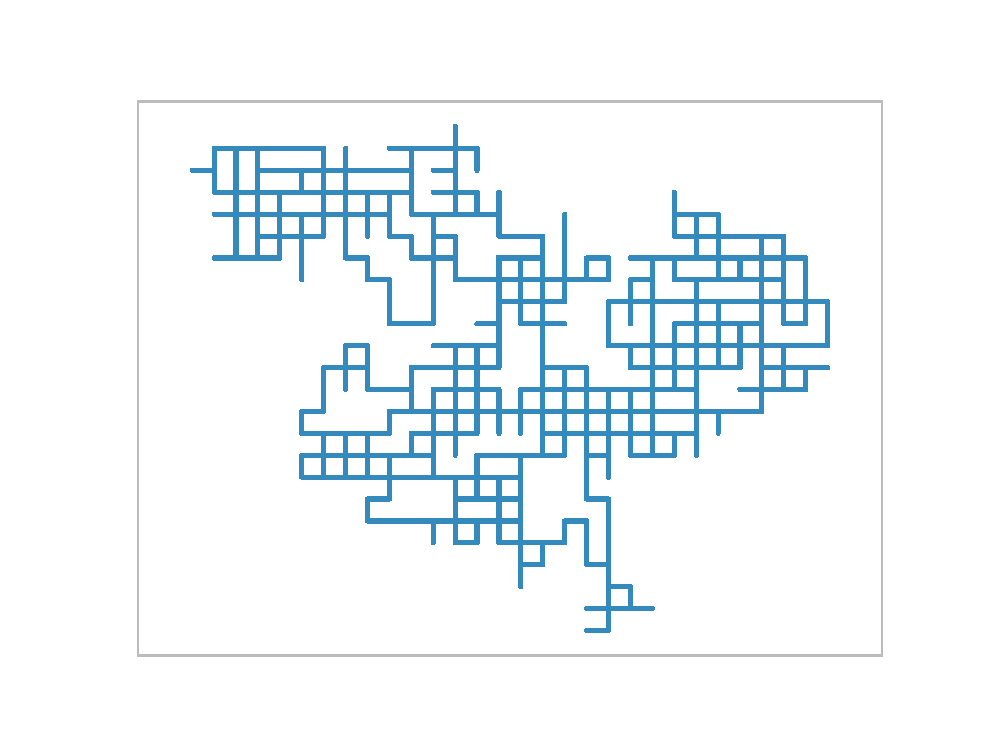
\includegraphics[scale=0.6]{../Images/randomwalk.eps}
	\caption{Random walker on a two-dimensional grid, 1000 moves.}
\end{figure}

Quantum Monte Carlo methods (QMC) represent a variety \textit{ab initio} methods that attempt to solve the Schrödinger equation using stochastic Monte Carlo integration. \textit{Ab initio} reads "from first principles", which implies that the methods constitute a fundamental approach to the problem. They all seek to evaluate the multi-dimensional integrals that represent various quantum mechanical expectation values. The expression for the energy reads
\begin{empheq}[box={\mybluebox[5pt]}]{equation}
E_0= \mel{\Psi_0}{\hat{\mathcal{H}}}{\Psi_0}= \frac{\int d\bs{X}\Psi_0(\bs{X})^*\hat{\mathcal{H}}\Psi_0(\bs{X})}{\int d\bs{X}\Psi_0(\bs{X})^*\Psi_0(\bs{X})},
\label{eq:schrodingergroundstate}
\end{empheq}
which provides the ground state energy expectation value for the exact ground state wave function $\Psi_0(\bs{X})$ with $\bs{X}=\{\{\bs{r}_1,\sigma_1\},\{\bs{r}_2,\sigma_2\},\hdots,\{\bs{r}_N,\sigma_N\}\}$ as the collective coordinates of the $N$ particles. As aforementioned, this integral is analytically infeasible for more or less all interesting systems, evokes the need for numerical methods like QMC. As we will stick to ground state calculations, the wave function $\Psi(\bs{X})$ implies the many-body ground state wave function from this point.

In Monte Carlo integration, we use random numbers to evaluate integrals numerically. Typically, we want to estimate an expectation value $\langle\hat{O}\rangle$ by approximating the integral with the sum,
\begin{equation}
\langle \hat{O}\rangle\equiv\int_{-\infty}^{\infty}d\bs{x}P(\bs{x})\hat{O}(\bs{x})\approx\frac{1}{M}\sum_{i=1}^M\hat{O}(\bs{x}_i),
\label{eq:montecarlointegration}
\end{equation}
where $M$ is the number of \textit{Monte Carlo cycles} and the coordinates $\bs{x}_i$ are drawn randomly from the probability density function $P(\bs{x})$. A great advantage of the QMC methods, is that we obtain approximative ground state wave functions when solving equation \eqref{eq:schrodingergroundstate}, which by the fourth postulate of quantum mechanics allows estimations of the ground state expectation values associated with other operators as well. 

Two widely used QMC methods are the variational Monte Carlo method (VMC) and the diffusion Monte Carlo method (DMC), where the former is arguably the simplest of all the QMC methods. It attempts to solve the integrals in equation \eqref{eq:schrodingergroundstate} directly by varying parameters, with the support of the variational principle presented in section \ref{sec:variationalprinciple}. This makes VMC a comparably computationally cheap method, but the performance is usually not in the league of the best methods. Diffusion Monte Carlo, on the other hand, is computationally expensive, but is also potentially numerically exact, making it a preferred method when high accuracy is needed. At first glance, it might seems like a tradeoff where VMC is used when computational time is more important than the accuracy and DMC is used when the opposite is true. However, DMC requires a wave function input which is close to the exact wave function, forcing us first to run a VMC calculation to obtain this wave function before the DMC machinery can be started.

As VMC is our main focus in this work, it will be explained thoroughly in this chapter. After that, we will briefly explain the idea behind the DMC method, but since this method is not implemented, it will not be our main priority. To reveal the uncertainty of our results, we will also discuss some methods to estimate the errors, in particular, the blocking method.

\section{Variational Monte Carlo} \label{sec:vmc}
The variational Monte Carlo method (hereafter the VMC method) is today widely used when it comes to the study of ground state properties of quantum many-body systems. It makes use of Markov chain Monte Carlo methods, often abbreviated MCMC, where the particles are assumed to be moving in Markov chains controlled by Monte Carlo simulations. Going back to the variational principle in equation \eqref{eq:variationalprinciple}, one observes that by choosing an approved wave function, one gets an energy larger or equal to the ground state energy.

Before we present the mathematical framework of the method, we will restate the two big challenges in many-body physics, mentioned in the introduction:
\begin{enumerate}
	\item The correct many-body wave function is generally unavailable.
	\item The many-body energy expectation value is analytically infeasible for most systems.
\end{enumerate}
In this section, we will look at how the VMC method tackles these challenges. We start with discussing the trial wave function, and set up our trial wave function ansatz. Then, we define the local energy and explain how it is used to solve the energy integral using Monte Carlo integration. In the end, we will mention some common extensions to the VMC method. 

\subsection{The trial wave function} \label{sec:trial}
The trial wave function was mentioned in section \ref{sec:cusp}, but a detailed description of it will first be presented here. In VMC, we start from a wave function ansatz, which is our ground state wave function guess. This function is equipped with variational parameters, and in order to estimate the wave function accurately, the trial wave function needs to be able to approach the correct wave function as we vary the parameters. However, as the many-body wave function is NP-hard to calculate \supercite{troyer_computational_2005}, we will only be able to approximate it and for that reason the wave function is by many considered as the root of all evil in many-body physics. For fermionic systems, the standard trial wave function used in VMC is the Slater-Jastrow wave function. Given a set of variational parameters $\bs{\theta}$, it can be expressed as
\begin{empheq}[box={\mybluebox[5pt]}]{equation}
\Psi_T(\bs{X};\bs{\theta})=|\hat{S}(\bs{X};\bs{\theta})|J(\bs{X};\bs{\theta}),
\end{empheq}
where $|\hat{S}(\bs{X};\bs{\theta})|$ is a Slater determinant used to bake in the anti-symmetry discussed in section \ref{sec:symmetry} and $J(\bs{R};\bs{\theta})$ is a Jastrow factor used to model the electron-electron correlations. Recall that the general Slater determinant has the form
\begin{equation}
|\hat{S}(\bs{X};\bs{\theta})|=\frac{1}{\sqrt{N!}}
\begin{vmatrix}
\psi_1(\boldsymbol{r}_1,\sigma_1;\bs{\theta}) & \psi_2(\boldsymbol{r}_1,\sigma_1;\bs{\theta}) & \hdots & \psi_N(\boldsymbol{r}_1,\sigma_1;\bs{\theta})\\
\psi_1(\boldsymbol{r}_2,\sigma_2;\bs{\theta}) & \psi_2(\boldsymbol{r}_2,\sigma_2;\bs{\theta}) & \hdots & \psi_N(\boldsymbol{r}_2,\sigma_2;\bs{\theta})\\
\vdots & \vdots & \ddots & \vdots \\
\psi_1(\boldsymbol{r}_N,\sigma_N;\bs{\theta}) & \psi_2(\boldsymbol{r}_N,\sigma_N;\bs{\theta}) & \hdots & \psi_N(\boldsymbol{r}_N,\sigma_N;\bs{\theta})
\end{vmatrix},
\label{eq:variationalslater}
\end{equation}
where the single-particle function $\psi(\bs{r},\sigma;\bs{\theta})$ can be decomposed in a spatial part, $\phi(\bs{r};\bs{\theta})$ and a spin part, $\xi(\sigma)$, 
\begin{equation}
\psi(\bs{r},\sigma;\bs{\theta})=\phi(\bs{r};\bs{\theta})\otimes\xi(\sigma).
\end{equation}
\iffalse
This question was answered already in the introductory words to this chapter, where we claimed that the wave function is estimated as we estimate the ground state energy. This is a fundamental part of the theory where the wave function is optimized in order to minimize the energy, and for that reason, a precise wave function estimate is essential to obtain precise estimates of the observable.
Consequently, the trial wave function converges towards the correct wave function as the energy converges towards the minimum. The convergence of the model is dependent on the initial trial wave function guess, which hopefully is close to the exact wave function. The parameters $\bs{\theta}$ are then updated to minimize $\langle E_L\rangle$, such that the energy gets lower for each \textit{iteration}.

As a notice, the term \textit{iterations} should not be confused with the term \textit{cycles}. For each iteration, we run $M$ Monte Carlo cycles and then update the parameters. The parameter update is discussed in section \ref{sec:parameterupdate}.

\subsection{Splitting up the Slater determinant} \label{sec:splittingofslater}
In order to reduce the computational cost of the Slater determinant, we will split it up in a spin-up part and a spin-down part. The splitting was explained thoroughly by \citet{nissenbaum_stochastic_2008}, appendix I, and this section is heavily inspired by it. In real life, we cannot immediately tell if an electron has spin-up or spin-down, but since we in the code need to know which particles that have spin-up and spin-down, we simply decide that the first $N_{\uparrow}$ particles have spin up and the remaining particles have spin down. 

In addition to reduce the computational cost, splitting up the Slater determinant also makes it possible to factorize out the spin-part from the single-particle functions. Only the spatial part of the single particle functions contribute to the energies, such that we with advantage can get rid of the spin parts. Recall that the single-particle functions $\psi(\bs{r},\sigma)$, can be written as a tensor product between the spatial part $\phi(\bs{r})$ and the spin part $\xi(\sigma)$, 
\begin{equation}
\psi(\bs{r},\sigma)=\phi(\bs{r})\otimes\xi(\sigma) 
\end{equation}
\fi
The tensor product is denoted by $\otimes$, and the factorization is only possible if the orbital and spin angular momenta of the particle are separable in the Hamiltonian underlying the system's dynamics. We will skip the tensor product notation in the following, but it is implicit that it is there. We also drop the $\bs{\theta}$ argument of the single-particle functions. As we in the ground state have double degeneracy, the spatial part will be the same for pairwise spin-up and spin-down particles, and we arrange them as
\begin{equation}
\psi_j(\bs{r}_i,\sigma_i)=
\begin{cases}
\phi_j(\bs{r}_i)\xi_{\uparrow}(\sigma_i)\quad\quad&\text{if } j<N_{\uparrow}\\
\phi_j(\bs{r}_i)\xi_{\downarrow}(\sigma_i)\quad\quad&\text{if } j\geq N_{\uparrow}
\end{cases}.
\end{equation}
Since the first $N_{\uparrow}$ particles have spin up, $\sigma_i=\,\uparrow\quad\forall\quad i\in\{1,2,...,N_{\uparrow}\}$, and the remaining have spin down, we can now set up the Slater determinant in equation \eqref{eq:variationalslater} where each single-particle function is split in a spatial part and a spin part,
\begin{equation*}
|\hat{S}(\bs{X})|=\frac{1}{\sqrt{N!}}
\begin{vmatrix}
\phi_1(\boldsymbol{r}_1)\xi_{\uparrow}(\uparrow) & \hdots & \phi_{N_{\uparrow}}(\boldsymbol{r}_1)\xi_{\uparrow}(\uparrow) & \phi_{1}(\boldsymbol{r}_1)\xi_{\downarrow}(\uparrow) & \hdots & \phi_{N_{\downarrow}}(\boldsymbol{r}_1)\xi_{\downarrow}(\uparrow)\\
\vdots & & \vdots & \vdots & & \vdots \\
\phi_1(\boldsymbol{r}_{N_{\uparrow}})\xi_{\uparrow}(\uparrow) & \hdots & \phi_{N_{\uparrow}}(\boldsymbol{r}_{N_{\uparrow}})\xi_{\uparrow}(\uparrow) & \phi_{1}(\boldsymbol{r}_{N_{\uparrow}})\xi_{\downarrow}(\uparrow) & \hdots & \phi_{N_{\downarrow}}(\boldsymbol{r}_{N_{\uparrow}})\xi_{\downarrow}(\uparrow)\\
\phi_1(\boldsymbol{r}_{N_{\uparrow}+1})\xi_{\uparrow}(\downarrow) & \hdots & \phi_{N_{\uparrow}}(\boldsymbol{r}_{N_{\uparrow}+1})\xi_{\uparrow}(\downarrow) & \phi_{1}(\boldsymbol{r}_{N_{\uparrow}+1})\xi_{\downarrow}(\downarrow) & \hdots & \phi_{N_{\downarrow}}(\boldsymbol{r}_{N_{\uparrow}+1})\xi_{\downarrow}(\downarrow)\\
\vdots & & \vdots & \vdots & & \vdots \\
\phi_1(\boldsymbol{r}_N)\xi_{\uparrow}(\downarrow) & \hdots & \phi_{N_{\uparrow}}(\boldsymbol{r}_N)\xi_{\uparrow}(\downarrow) & \phi_{1}(\boldsymbol{r}_N)\xi_{\downarrow}(\downarrow) & \hdots & \phi_{N_{\downarrow}}(\boldsymbol{r}_N)\xi_{\downarrow}(\downarrow)\\
\end{vmatrix}.
\end{equation*}
We observe that the the spin-up particles sometimes occupy spin-down states, which they are not allowed to. Therefore, half of the elements become zero and the determinant can be further expressed as
\begin{equation*}
|\hat{S}(\bs{X})|=\frac{1}{\sqrt{N!}}
\begin{vmatrix}
\phi_1(\boldsymbol{r}_1)\xi_{\uparrow}(\uparrow) & \hdots & \phi_{N_{\uparrow}}(\boldsymbol{r}_1)\xi_{\uparrow}(\uparrow) & 0 & \hdots & 0\\
\vdots & & \vdots & \vdots & & \vdots \\
\phi_1(\boldsymbol{r}_{N_{\uparrow}})\xi_{\uparrow}(\uparrow) & \hdots & \phi_{N_{\uparrow}}(\boldsymbol{r}_{N_{\uparrow}})\xi_{\uparrow}(\uparrow) & 0 & \hdots & 0\\
0 & \hdots & 0 & \phi_{1}(\boldsymbol{r}_{N_{\uparrow}+1})\xi_{\downarrow}(\downarrow) & \hdots & \phi_{N_{\downarrow}}(\boldsymbol{r}_{N_{\uparrow}+1})\xi_{\downarrow}(\downarrow)\\
\vdots & & \vdots & \vdots & & \vdots \\
0 & \hdots & 0 & \phi_{1}(\boldsymbol{r}_N)\xi_{\downarrow}(\downarrow) & \hdots & \phi_{N_{\downarrow}}(\boldsymbol{r}_N)\xi_{\downarrow}(\downarrow)\\
\end{vmatrix},
\end{equation*}
where the Slater matrix now is block diagonal! For a general block diagonal matrix, the determinant is given by the product of the determinant of each block
\begin{equation}
|\hat{S}(\bs{X})|=\frac{1}{\sqrt{N!}}|\hat{S}_{\uparrow}(\bs{X}^{\uparrow})|\cdot |\hat{S}_{\downarrow}(\bs{X}^{\downarrow})|,
\end{equation}
which can be seen by writing the total matrix as a product over all the block diagonal matrix. $\hat{S}_{\sigma}$ is the matrix containing all spin-$\sigma$ states with collective coordinates $\bs{X}^{\sigma}=\{\{\bs{r}_1^{\sigma},\xi_{\sigma}(\sigma)\},\{\bs{r}_2^{\sigma},\xi_{\sigma}(\sigma)\},\hdots,\{\bs{r}_N^{\sigma},\xi_{\sigma}(\sigma)\}\}$. Since all elements in the respective matrices contain the same spin function, it can be factorized out \supercite{nissenbaum_stochastic_2008},
\begin{equation}
\begin{aligned}
|\hat{S}(\bs{X})|=\frac{1}{\sqrt{N!}}&|\hat{D}_{\uparrow}(\bs{r}_1, \bs{r}_2,\hdots,\bs{r}_{N_{\uparrow}})|\{\xi_{\uparrow}(\sigma_1^{\uparrow})\xi_{\uparrow}(\sigma_2^{\uparrow})\hdots\xi_{\uparrow}(\sigma_{N_{\uparrow}}^{\uparrow})\}, \\ \times&|\hat{D}_{\downarrow}(\bs{r}_{N_{\uparrow}+1}, \hdots,\bs{r}_{N-1},\bs{r}_{N})|\{\xi_{\downarrow}(\sigma_{N_{\uparrow}+1}^{\downarrow})\hdots\xi_{\downarrow}(\sigma_{N-1}^{\downarrow})\xi_{\downarrow}(\sigma_{N}^{\downarrow})\},
\end{aligned}
\end{equation}
and omitted in the future study. We can then define a set, $\bs{R}^{\sigma}=\{\bs{r}_1^{\sigma},\bs{r}_2^{\sigma},\hdots,\bs{r}_N^{\sigma}\}$, containing the spatial coordinates of the spin-$\sigma$ particles and $\bs{R}=\{\bs{r}_1,\bs{r}_2,\hdots,\bs{r}_N\}$ containing the collective spatial coordinates. The Slater determinant we are left with is thus
\begin{empheq}[box={\mybluebox[5pt]}]{equation}
|\hat{S}(\bs{R})|=\frac{1}{\sqrt{N!}}|\hat{S}_{\uparrow}(\bs{R}^{\uparrow})|\cdot |\hat{S}_{\downarrow}(\bs{R}^{\downarrow})|,
\end{empheq}
which is independent of spin, i.e. the matrices now consist of the spatial functions $\phi_j(\bs{r}_i)$ as the elements,
\begin{equation}
|\hat{S}_{\sigma}(\bs{R}^{\sigma})|=
\begin{vmatrix}
\phi_1(\boldsymbol{r}_1^{\sigma}) & \phi_2(\boldsymbol{r}_1^{\sigma}) & \hdots & \phi_{N}(\boldsymbol{r}_1^{\sigma})\\
\phi_1(\boldsymbol{r}_2^{\sigma}) & \phi_2(\boldsymbol{r}_2^{\sigma}) & \hdots & \phi_{N}(\boldsymbol{r}_2^{\sigma})\\
\vdots & \vdots & & \vdots \\
\phi_1(\boldsymbol{r}_{N}^{\sigma}) & \phi_2(\boldsymbol{r}_{N}^{\sigma}) & \hdots & \phi_{N}(\boldsymbol{r}_{N}^{\sigma})
\end{vmatrix}.
\end{equation}

It is also worth to notice that the number of spin-up particles determines the size of the spin-up matrix, and the number of spin-down particles determines the size of the spin-down matrix. In other words, we can change the ratio between spin-up particles and spin-down particles by adjusting the relative sizes of the determinants. In the implementation, however, we stick to the magic quantum numbers, where $N_{\uparrow}=N_{\downarrow}$.

\subsection{The Jastrow factor} \label{sec:jastrow}
The second factor in our trial wave function ansatz is the Jastrow factor, which is added in order to account for the electron-electron correlations. As discussed the section \ref{sec:cusp}, it is crucial to model the so-called cusps correctly, which is the task of the Jastrow factor. We will first discuss a simple Jastrow factor, and then move on the the more complex Padé-Jastrow factor. 

\subsubsection{Simple Jastrow} \label{sec:simplejastrow}
The simple Jastrow factor is just an exponential function with the sum over all particle distances. In addition, each distance $r_{ij}$ is weighted by a parameter $\beta_{ij}$, and the factor becomes
\begin{equation}
J(\bs{r}; \bs{\beta}) = \exp(\sum_{i=1}^N\sum_{j>i}^N{\beta_{ij}r_{ij}}).
\label{eq:SimpleJastrow}
\end{equation}
All the $\beta_{ij}$ are free variational parameters, which are expected to be symmetric since the distance matrix is symmetric. 

\subsubsection{Padé-Jastrow} \label{sec:padejastrow}
The Padé-Jastrow factor is closely related to the simple Jastrow above, but a numerator makes it more complex. It reads
\begin{equation}
J(\bs{r};\beta) = \exp(\sum_{i=1}^N\sum_{j>i}^N\frac{a_{ij}r_{ij}}{1+\beta r_{ij}}).
\label{eq:PadeJastrow}
\end{equation}
where $\beta$ is a variational parameter. In addition, the fractions are multiplied with factors $a_{ij}$ which depend on the particles $i$ and $j$ in the following way:
\begin{equation}
\label{eq:ajastrow}
a_{ij}=
\begin{cases} 
1/(d+1) & \text{if $i,j$ are particles of same spin}, \\
1/(d-1) & \text{if $i,j$ are particles of opposite spin},
\end{cases}
\end{equation}
for dimensions $d\in\{2,3\}$ where the natural units are used. For two dimensions, this gives $a_{ij}=1/3$ (same spin) or $a_{ij}=1$ (opposite spin) and for three dimensions $a_{ij}=1/4$ (same spin) and $a_{ij}=1/2$ (opposite spin) \supercite{hogberget_quantum_2013,mariadason_quantum_2018}. These values are determined by the cusp condition\supercite{bingel_a_physical_1967}.

\subsection{The local energy}
We have now seen how we approximate the wave function by a trial wave function, and in this section we will describe how to find the energy. In chapter \ref{chp:quantum}, we saw that the two-body interaction term makes the integral impossible to solve analytically for many particles, such that we need to rely on numerical methods. 

As we have seen, in VMC, we start with a trial wave function guess $\Psi_T(\bs{R};\bs{\theta})$ where the parameters $\bs{\theta}$ are varied to minimize the energy. According to the variational principle, the obtained energy will always be higher or equal to the true ground state energy, where the equality is the case if and only if the wave function is the exact ground state wave function. Denoting the exact ground state energy by $E_0$ and the obtained energy as $E$, we can summarize this by
\begin{equation}
E_0 \leq E = \frac{\int d\bs{R}\Psi_T(\bs{R})^*\hat{\mathcal{H}}\Psi_T(\bs{R})}{\int d\bs{R}\Psi_T(\bs{R})^*\Psi_T(\bs{R})}.
\end{equation}
Furthermore, the integral can be written in the form of a general expectation value,
\begin{equation}
E = \int d\bs{R} E_L(\bs{R})P(\bs{R}),
\end{equation}
defining the local energy as
\begin{equation}
E_L(\bs{R})\equiv\frac{1}{\Psi_T(\bs{R})}\hat{\mathcal{H}}\Psi_T(\bs{R})
\label{eq:localenergy}.
\end{equation}
$P(\bs{R})$ is called the probability density function (PDF) and was first introduced in equation \eqref{eq:pdf}. In a more general scheme the PDF reads
\begin{equation}
P(\bs{R})=\frac{|\Psi_T(\bs{R})|^2}{\int d\bs{R}|\Psi_T(\bs{R})|^2},
\label{eq:probvmc}
\end{equation}
where the wave function is not necessarily normalized. Since the energy expectation value now is in the form of a general expectation value, we can use the approximation set up by Monte Carlo integration in equation \eqref{eq:montecarlointegration}, yielding 
\begin{empheq}[box={\mybluebox[5pt]}]{equation}
E \approx \frac{1}{M}\sum_{i=1}^ME_L(\bs{R}_i),
\label{eq:energysum}
\end{empheq}
where the local energies $E_L(\bs{R}_i)$ are still evaluated with particle coordinates $\bs{R}_i$ drawn from $P(\bs{R})$. In this manner, the obtained energy is guaranteed to approach the exact energy as the number of Monte Carlo cycles, $M$, increases. Actually, the standard error goes as $\mathcal{O}(1/\sqrt{M})$, making the method pretty accurate for large $M$'s. In the limit $M\rightarrow\infty$, the error goes to zero,
\begin{equation}
\langle E_L\rangle=\lim_{M\to\infty} \frac{1}{M}\sum_{i=1}^ME_L(\bs{R}_i),
\end{equation}
indicating the need for a large number of cycles. This is associated with a zero-variance property governing the quantum Monte Carlo methods, stating that the variance in the true ground state should be zero \supercite{deb_variational_2014, assaraf_zero-variance_2003}. Various sampling regimes are described in section \ref{sec:metropolis}.

\subsection{Parameter update} \label{sec:parameterupdate}
Above we have discussed the sampling in detail, which is a central part of the VMC method. Another important part is the update of the parameters, which we need in order to find an approximative wave function. In section \ref{sec:optimizationalgorithms}, we discussed various gradient-based optimization algorithms for iterative minimization of the cost function $\mathcal{C}(\bs{\theta})$ in machine learning, and the same methods can be used in VMC.

However, we need to define a cost function for VMC which is minimized when the ground state energy is obtained. According to the variational principle, the ground state energy is the lowest energy we can obtain, so an obvious cost function is the energy expectation value. We therefore set
\begin{equation}
\mathcal{C}(\bs{\theta})=\langle E_L\rangle,
\end{equation}
since we get the expectation value of the local energy from the Metropolis sampling. Further, we use the definition of the gradient of an expectation value from \citet{umrigar_energy_2005} and obtain
\begin{empheq}[box={\mybluebox[5pt]}]{equation}
\nabla_{\theta_j} \langle E_L\rangle=2\Big(\langle E_L\nabla_{\theta_j}\ln\Psi_T\rangle - \langle E_L\rangle\langle\nabla_{\theta_j}\ln\Psi_T\rangle\Big),
\label{eq:gradientenergy}
\end{empheq}
which means that we need to calculate the expectation values $\langle E_L\nabla_{\theta_j}\ln\Psi_T\rangle$ and $\langle\nabla_{\theta_j}\ln\Psi_T\rangle$ in addition to the expectation value of the local energy. These expectation values are found from the integrals
\begin{equation}
\langle\nabla_{\theta_j}\ln\Psi_T\rangle = \int_{-\infty}^{\infty}d\bs{R}\nabla_{\theta_j}\ln\Psi_T(\bs{R})P(\bs{R}),
\end{equation}
and
\begin{equation}
\langle E_L\nabla_{\theta_j}\ln\Psi_T\rangle = \int_{-\infty}^{\infty}d\bs{R}E_L(\bs{R})\nabla_{\theta_j}\ln\Psi_T(\bs{R})P(\bs{R}),
\end{equation}
which can be found by Monte Carlo integration in the same way as the local energy:
\begin{equation}
\langle\nabla_{\theta_j}\ln\Psi_T\rangle\approx \frac{1}{M}\sum_{i=1}^M\nabla_{\theta_j}\ln\Psi_T(\bs{R}_i)
\end{equation}
and
\begin{equation}
\langle E_L\nabla_{\theta_j}\ln\Psi_T\rangle\approx \frac{1}{M}\sum_{i=1}^ME_L(\bs{R}_i)\nabla_{\theta_j}\ln\Psi_T(\bs{R}_i).
\end{equation}
Note that the only closed-form expression needed, in addition to the local energy, is the expression of $\nabla_{\theta_j}\ln\Psi_T(\bs{R}_i)$. This will later be found for the various wave functions. 

We want to stress that the local energy is not the only possible choice of cost function. By taking advantage of the zero-variance property of the expectation value of the local energy in the minimum, one can also minimize the variance. Variance minimization requires the calculation of a few additional expectation values, but it is a fully manageable task to do. See for instance \citet{bajdich_electronic_2010} for more information.

\subsection{The electron density} \label{sec:electrondensityqmc}
In section \ref{sec:electrondensity}, we introduced the electron density and defined the $P$-body density as an integral over all particles but $P$,
\begin{equation}
\rho_P(\bs{r}_1,\hdots,\bs{r}_P)=N\int_{-\infty}^{\infty}d\bs{r}_{P+1}\hdots d\bs{r}_N |\Psi(\bs{r}_1,\hdots \bs{r}_N)|^2.
\end{equation}
Not surprising, also this integral will be solved using Monte Carlo integration, but in a slightly different way than the integrals above since this integral returns a distribution rather than an expected value. First, we divide the space into bins which either have equal sizes or known sizes. After that, we sample the particles and count the number of times a particle occurs in each bin. We want to find the relative number of particles in each bin concerning the size of the bin, so if the bins are of different sizes, we need to standardize them all by dividing by their respective sizes. In the end, we normalize the density such that the sum of all densities becomes equal to $N$. This method and the particular implementation is detailed in section \ref{sec:electrondensityimplementation}.

\subsection{Common extensions}
This finalizes the essential theory behind the VMC method. However, a sampling algorithm is needed to draw samples randomly from $P(\bs{R})$, and in section \ref{sec:metropolis} some popular sampling techniques are described. Before we jump into this field, we will discuss some natural extensions and improvements to the VMC method.

Initially, the particle configuration $\bs{R}$ might not be representative for a configuration in equilibrium, making the first cycles a poor estimate of the expectation value. An easy fix to this problem is to basically ignore the first sampling period, known as the \textit{burn-in period}. With this in mind, we can implement an equilibration fraction describing the fraction of the total number of cycles that are used in the burn-in period. When running multiple parallel processes, the burn-in period should be the same for all the processes.

We also have a technique called \textit{thinning}, which means picking every $n$'th sample in the chain and ignore the rest. This is shown to give a more or less identical expectation value and makes the program less memory-requiring, but due to worse statistics, this should be avoided as long as there is no lack of memory. 

\section{Unifying Quantum Mechanics and Machine Learning} \label{sec:unifying}
Now as we have introduced the necessary theory, both in the form of quantum theory and machine learning theory, in addition to detailing the variational Monte Carlo (VMC) method, we are ready to unify the machine learning and quantum mechanics. As hinted above, the way we do this is to let a restricted Boltzmann machine define our single-particle functions in the trial wave function, and then just update the function in a normal VMC scheme. This is very similar to the approach of \citet{pfau2019abinitio}, but an essential difference is that they also used the relative distances between the particles as inputs to the neural network. Further, we investigate how the results change when Jastrow factors with increasing amount of physical intuition are added. As the main goal is to find a method that requires less physical intuition in order to provide accurate results compared to the traditional methods, adding a simple Jastrow factor is also very interesting. We look at three different trial wave function ansätze for the Boltzmann machines: a Slater determinant where the single-particle functions are given by the marginal distribution of the visible units of a Gaussian-binary restricted Boltzmann machine (RBM), an RBM with a simple Jastrow added (RBM+SJ) and an RBM with a Padé-Jastrow factor added (RBM+PJ). They are detailed in respective sections below.

\subsection{Restricted Boltzmann machine without Jastrow factor (RBM)} \label{sec:rbm}
In section \ref{sec:trial}, we saw how the VMC method attempts to solve the time-independent Schrödinger equation directly by varying the parameters in a trial wave function. In order to satisfy the anti-symmetry properties of a fermionic many-body wave function, the trial wave function was composed as a Slater determinant,
\begin{equation}
|\hat{S}(\bs{R})|=\frac{1}{\sqrt{N!}}|\hat{S}_{\uparrow}(\bs{R}^{\uparrow})|\cdot |\hat{S}_{\downarrow}(\bs{R}^{\downarrow})|,
\end{equation}
where
\begin{equation}
|\hat{S}_{\sigma}(\bs{R})|=
\begin{vmatrix}
\phi_1(\boldsymbol{r}_1) & \phi_2(\boldsymbol{r}_1) & \hdots & \phi_N(\boldsymbol{r}_1)\\
\phi_1(\boldsymbol{r}_2) & \phi_2(\boldsymbol{r}_2) & \hdots & \phi_N(\boldsymbol{r}_2)\\
\vdots & \vdots & \ddots & \vdots \\
\phi_1(\boldsymbol{r}_N) & \phi_2(\boldsymbol{r}_N) & \hdots & \phi_N(\boldsymbol{r}_N)
\end{vmatrix}.
\end{equation}
Even though we want a method which requires as little physical intuition as possible, the wave function needs to obey Fermi-Dirac statistics, and we therefore also approximate the trial wave function with the Slater determinant for the machine learning methods. Further, we use the same framework as we did for VMC, but the single-particle functions (SPFs) $\phi_j(\bs{r}_i)$ are given by the marginal distribution of the visible units from a restricted Boltzmann machine, $P(\bs{r})$. For quantum dots, we also add the Hermite polynomials, $H_n(\bs{r})$ to get a unique SPF for each state. We then have
\begin{equation}
\phi_j(\bs{r}_i)=H_j(\bs{r}_i)P(\bs{r}_i),
\end{equation}
where the marginal distribution is the distribution obtained in equation \eqref{eq:RBMWF2}. The RBM trial wave function is then simply
\begin{equation}
\Psi_T(\bs{R})=|\hat{S}_{\uparrow}(\bs{R}^{\uparrow})|\cdot |\hat{S}_{\downarrow}(\bs{R}^{\downarrow})|,
\end{equation}
where we omit the normalization factor, $Z$, as it is not required by the method, as we will see in section \ref{sec:metropolis}.

\subsection{RBM with a simple Jastrow factor (RBM+SJ)} \label{sec:rbmsj}
This method, abbreviated RBM+SJ, is just an extension of the RBM method described in the previous section, where we add the simple Jastrow factor described in section \ref{sec:jastrow} to help modeling the electron-electron cusp. When adding a Jastrow factor we also add some more physical intuition to the trial wave function, but the Jastrow factor used here still contains a minimum of physical intuition. The trial wave function using this method thus takes the form
\begin{equation}
\Psi_T(\bs{R})=|\hat{D}_{\uparrow}(\bs{R}^{\uparrow})|\cdot|\hat{D}_{\downarrow}(\bs{R}^{\downarrow})|J(\bs{R};\bs{\beta}),
\end{equation}
where $\bs{\beta}$ is a set of variational parameters and where the normalization factor, $Z$, again is omitted.  

\subsection{RBM with a Padé-Jastrow factor (RBM+PJ)} \label{sec:rbmpj}
Lastly, we add the well-known Padé-Jastrow factor to the RBM, abbreviated RBM+PJ, to see how much the results change when a more advanced correlation factor is added. As discussed in section \ref{sec:jastrow}, the Padé-Jastrow factor is constructed to model the electron-electron cusp correctly, and it is also interesting to see how an increased amount of physical intuition in the trial wave function affects the results. The RBM+PJ trial wave function then reads
\begin{equation}
\Psi_T(\bs{R})=|\hat{D}_{\uparrow}(\bs{R}_{\uparrow})|\cdot|\hat{D}_{\downarrow}(\bs{R}_{\downarrow})|J(\bs{R};\beta),
\end{equation}
where we recall that the Padé-Jastrow factor contains the variational parameter $\beta$.

\section{The Metropolis Algorithm} \label{sec:metropolis}
Metropolis sampling is a Markov chain Monte Carlo method, which generates a Markov chain using a proposal density for new steps, and the method also rejects unsatisfying moves. In its most simple form, a particle is moved in a random direction, which was the original method invented by \citet{metropolis_equation_1953} back in 1953. Later, the method was improved by \citet{hastings_monte_1970}, giving rise to the more general Metropolis-Hastings algorithm. The genius of the Metropolis algorithms is that the acceptance of a move is not based on the probabilities themselves, but rather the ratio between the new and the old probabilities. In that way, we avoid calculating the normalizing factor, which is often computationally intractable.

We will first discuss Markov chains in general, before we connect them to the original Metropolis algorithm, henceforth called \textit{brute-force sampling}, and then the Metropolis-Hastings algorithm, also called \textit{importance sampling}. If we denote the current state by $\bs{R}$, and the proposed state by $\bs{R}'$, we have a transition rule $P(\bs{R}'|\bs{R})$ for going from $\bs{R}$ to $\bs{R}'$ and a transition rule $P(\bs{R}|\bs{R}')$ for going the opposite way. If we then assume that the rules satisfy \textit{ergodicity} and \textit{detailed balance}, we have the following relationship:
\begin{equation}
P(\bs{R}'|\bs{R})P(\bs{R})=P(\bs{R}|\bs{R}')P(\bs{R}'),
\end{equation}
which is actually a restatement of Bayes' theorem presented in section \ref{sec:bayes}. The next step is to rewrite the transition rules in terms of a proposal distribution $T(\bs{R}'|\bs{R})$ and an acceptance probability $A(\bs{R}',\bs{R})$,
\begin{equation}
P(\bs{R}'|\bs{R})=T(\bs{R}'|\bs{R})A(\bs{R}',\bs{R}).
\end{equation}
In order to satisfy the detailed balance, we need to choose $A(\bs{R}',\bs{R})$ such that
\begin{empheq}[box={\mybluebox[5pt]}]{equation}
A(\bs{R}',\bs{R})=\text{min }\left[1,\frac{T(\bs{R}|\bs{R}')P(\bs{R}')}{T(\bs{R}'|\bs{R})P(\bs{R})}\right],
\label{eq:acceptance}
\end{empheq}
where we limit $A$ to maximum 1 as the probability should not exceed 1. We want to accept a move with probability $A(\bs{R}',\bs{R})$. One way to do that is to draw a number from a uniform distribution between 0 and 1. If this number is lower than the acceptance, the move should be accepted and if not, the move should be rejected.

\subsection{Brute-force sampling} \label{sec:bruteforce}
In its simplest form, the move is proposed randomly both in magnitude and direction. Mathematically, we can write this as
\begin{equation}
\bs{R}'=\bs{R}+\Delta xd\bs{R},
\end{equation}
where $\Delta x$ is the step length and $d\bs{r}$ has a random magnitude and direction (typically which particle to move). We obtain the naïve acceptance probability when requiring $T(\bs{R}'|\bs{R})=T(\bs{R}|\bs{R}')$, such that it simplifies to
\begin{empheq}[box={\mybluebox[5pt]}]{equation}
A(\bs{R}',\bs{R})=\text{min }\left[1,\frac{P(\bs{R}')}{P(\bs{R})}\right].
\end{empheq}
However, with this approach, an unsatisfying number of moves will be rejected as the particles can be moved in all directions, which results in a significant waste of computing power. A better method is \textbf{importance sampling}, since the particles are moved according to the so-called quantum force to be defined below. 

\subsection{Importance sampling} \label{sec:importancesampling}
Importance sampling is a more intelligent sampling method than the brute-force sampling, since the new position is based on an educated guess. To understand how it works, we need to take a quick look at diffusion processes. We start from the Fokker-Planck equation,
\begin{equation}
\frac{\partial P(\bs{R},t)}{\partial t}=D\nabla\left(\nabla-\bs{F}\right)P(\bs{R},t),
\label{eq:fokkerplanck}
\end{equation}
which describes how a probability distribution $P(\bs{R},t)$ evolves in appearance of a drift force $\bs{F}$. In the case $\bs{F}=\bs{0}$, the equation reduces to the diffusion equation with $D$ as the diffusion constant. This simplifies to $D=1/2$ in natural units. 

The Langevin equation states that a diffusion particle tends to move parallel to the drift force in the coordinate space, with $\bs{\eta}$ introducing some random noise. The equation reads
\begin{equation}
\frac{\partial \bs{R}(t)}{\partial t}=D\bs{F}(\bs{R}(t))+\bs{\eta}.
\label{eq:langevin}
\end{equation}
Given a position $\bs{R}$, the new position $\bs{R}'$ can be be found by applying forward-Euler on the Langevin equation, obtaining
\begin{equation}
\bs{R}'=\bs{R}+D\Delta t\bs{F}(\bs{R}) + \bs{\xi}\sqrt{\Delta t},
\end{equation}
where $\Delta t$ is a fictive time step and $\bs{\xi}$ is a Gaussian random variable. Further, we want to find an expression of the drift force $\bs{F}$ which makes the system converge to a stationary state. A stationary state is found when the probability density function, $P(\bs{R})$, is constant in time, i.e. when the left-hand side of the Fokker-Planck equation is zero. In that case, we can rewrite the equation as
\begin{equation}
\nabla^2P(\bs{R})=P(\bs{R})\nabla\bs{F}(\bs{R})+\bs{F}(\bs{R})\nabla P(\bs{R}),
\end{equation}
where the parenthesis are written out and we have moved the term that is independent of the force $\bs{F}$ to the left-hand side. Moreover, we assume that the drift force takes the form $\bs{F}(\bs{R})=g(\bs{R})\nabla P(\bs{R})$ based on the fact that the force should point in the direction of the steepest slope. We can then go ahead and write
\begin{equation}
\nabla^2 P(\bs{R})\big(1-P(\bs{R})g(\bs{R})\big)=\nabla\big(g(\bs{R})P(\bs{R})\big)\nabla P(\bs{R}),
\end{equation}
where the quantity $\nabla^2 P(\bs{R})$ is factorized out from two of the terms. The equation is satisfied when $g(\bs{R})=1/P(\bs{R})$, such that the drift force evolves to the well-known form
\begin{equation}
\bs{F}(\bs{R})=\frac{\nabla P(\bs{R})}{P(\bs{R})}=2\frac{\nabla\Psi_T(\bs{R})}{\Psi_T(\bs{R})}=2\nabla\ln\Psi_T(\bs{R}),
\end{equation}
which is also known as the \textit{quantum force}. 

The remaining part concerns the acceptance of the moves. For this, we need to find the sampling distributions $T(\bs{R}'|\bs{R})$ from equation \eqref{eq:acceptance}, which are just the solutions of the Fokker-Planck equation. The solutions read
\begin{equation}
G(\bs{R}',\bs{R},\Delta t)\frac{1}{(4\pi D\Delta t)^{3N/2}}\exp\Big(-\big(\bs{R}'-\bs{R}-D\Delta t\bs{F}(\bs{R})\big)^2/4D\Delta t\Big),
\end{equation}
which is categorized as a Green's function. In general, the essential property of any Green's function is that it provides a way to describe the response of an arbitrary differential equation solution. For our particular case, it correspond to $\mathcal{N}(\bs{R}'|\bs{R}+D\Delta t \bs{F}(\bs{R}),2D\Delta t)$ which is the normal distribution with mean $\bs{\mu}=\bs{R}+D\Delta t \bs{F}(\bs{R})$ and variance $\sigma=2D\Delta t$. By using this, the acceptance probability of the importance sampling can finally be written as
\begin{empheq}[box={\mybluebox[5pt]}]{equation}
A(\bs{R}'|\bs{R})=\text{min }\left[1,\frac{G(\bs{R},\bs{R}',\Delta t)P(\bs{R}')}{G(\bs{R}',\bs{R}, \Delta t)P(\bs{R})}\right],
\end{empheq}
where the marginal probabilities are still given by equation \eqref{eq:probvmc}. 

\subsection{Gibbs sampling}
Gibbs sampling has, throughout the years, gained high popularity in the machine learning community when it comes to training Boltzmann machines. There are probably many factors that contribute to this, where the performance is one of them. Another proper motivation is the absence of tuning parameters, which makes the method more comfortable to deal with compared to many of its competitors. The method is an instance of the Metropolis-Hastings algorithm and is therefore classified as another Markov chain Monte Carlo method. It differs from the Metropolis methods discussed above by the fact that all the moves are accepted, such that we do not waste computational time on rejected moves. Nevertheless, we should not use this argument alone to motivate the use of Gibbs sampling, as the algorithm usually and preferably rejects less than 1\% of the moves in importance sampling.

We will in the following briefly describe the mathematical foundation of the method, before we, for the sake of clarity, connect it to the restricted Boltzmann machines. The method is built on the concept that, given a multivariate distribution, it is simpler to sample from a conditional distribution than to marginalize by integrating over a joint distribution. This is the reason why we do not need the marginal distributions in Gibbs sampling, but rather the conditional distributions. In the most general case, Gibbs sampling proposes a rule for going from a sample $\bs{x}^{(i)}=\{x_1^{(i)},x_2^{(i)},\hdots,x_n^{(i)}\}$ to another sample $\bs{x}^{(i+1)}=\{x_1^{(i+1)},x_2^{(i+1)},\hdots,x_n^{(i+1)}\}$, similar to the Metropolis algorithm. However, in Gibbs sampling the transition from $x_j^{(i)}$ to $x_j^{(i+1)}$ is performed according to the conditional distribution specified by
\begin{equation}
P\big(x_j^{(i+1)}|x_1^{(i+1)},\hdots,x_{j-1}^{(i+1)},x_{j+1}^{(i)},\hdots,x_n^{(i)}\big).
\end{equation}
The marginal distribution of a subset of variables can then be approximated by simply considering the samples for that subset of variables, ignoring the rest. 

For a restricted Boltzmann machine, this becomes a two-step sampling process as we have two layers, such that we use the conditional probabilities $P(\bs{x}|\bs{h})$ and $P(\bs{h}|\bs{x})$ to update the visible and hidden units respectively. For the restricted Boltzmann machine with Gaussian-binary units presented in section \ref{sec:RBM}, the conditional probability of $h_j=0$ given a set of visible nodes $\bs{x}$ is
\begin{equation}
P(h_j=0|\bs{x})=\frac{1}{1+\exp(+b_j+\sum_{i=1}^Nx_iw_{ij}/\sigma_i^2)},
\end{equation}
and the corresponding conditional probability of $h_j=1$ is
\begin{equation}
P(h_j=1|\bs{x})=\frac{1}{1+\exp(-b_j-\sum_{i=1}^Nx_iw_{ij}/\sigma_i^2)},
\end{equation}
which is by the way again the sigmoid. Note that $P(h_j=0|\bs{x})+P(h_j=1|\bs{x})=1$, indicating that a hidden node, $h_j$, can only take the values 0 or 1. When updating the hidden node, we typically calculate the sigmoid $P(h_j=1|\bs{x})$ and set $h_j$ to 1 if this probability is larger than 1/2, and set it to 0 otherwise. 

For the update of the visible nodes, we see from equation \eqref{eq:normal} that the visible nodes are chosen after the normal distribution,
\begin{equation}
P(x_i|\bs{h})=\mathcal{N}\left(a_i+\sum_{j=1}^Hw_{ij}h_j,\sigma_i^2\right),
\end{equation}
which introduces some stochasticity to the system. By going back and forth in the Boltzmann machine multiple times (a round trip corresponds to an iteration), the hope is that the expectation values can be approximated by averaging over all the iterations. 

As pointed out earlier, the Gibbs sampling will not be implemented in this work, but we describe it for completeness purposes. The reason for this is that the method has not shown promising results for our specific problem, and we will instead rely on Metropolis sampling. We have already tested the Gibbs sampling in another similar project on small quantum dots \supercite{nordhagen_computational_2018}, and so have others like \citet{flugsrud_vilde_moe_solving_nodate}. The results are matching and show poor performance compared to the Metropolis-Hastings algorithm.

However, the Gibbs sampling method should not be underestimated. \citet{carleo_solving_2017} showed its importance when solving the Ising model using a restricted Boltzmann machine and Gibbs sampling, and in traditional Boltzmann machines, the Gibbs sampling is the preferred tool.

\section{Diffusion Monte Carlo} \label{sec:dmc}
The second and last quantum Monte Carlo method we will discuss is the diffusion Monte Carlo (DMC) method. DMC belongs to a class of projection and Green's function approaches and provides in principle an exact solution of the Schrödinger equation. However, for fermionic systems, the method is plagued by the occurrence of a sign-problem, known as the fermion sign problem \supercite{troyer_computational_2005}, and we need to use approximations to bypass the problem. The most common fix is the fixed-node approximation, which introduces errors to the computations. The problem is also attempted to solve using shadow wave functions, for instance, by \citet{calcavecchia_sign_2014}, which have many commonalities with our restricted Boltzmann machine (RBM) approach. The idea is that the RBMs can also contribute to solve the sign problem, but we leave this for later studies. 

Since the DMC method is used as a reference for more or less all the produced results, it is natural to give a brief discussion of the idea behind the method. By the fifth postulate of quantum mechanics discussed in section \ref{sec:postulates}, the motion of a particle that moves in a potential $V(\bs{R})$ is described by the time-dependent Schrödinger equation,
\begin{equation}
i\frac{\partial\Psi(\bs{R},t)}{\partial t}=\hat{\mathcal{H}}\Psi(\bs{R},t),
\end{equation}
with $\Psi(\bs{R},t)$ as the many-body wave function, $t$ as the time and $i$ as the solution of $x^2=-1$. In natural units, the Hamiltonian is given by
\begin{equation}
\hat{\mathcal{H}}=-\frac{1}{2}\nabla^2 + V(\bs{R}).
\end{equation}
Further, we assume that the potential becomes infinite as $x\rightarrow \pm\infty$, such that the particle motion is confined to a finite spatial domain. The formal solution of the time-dependent Schrödinger equation is then given by an expansion of the eigenfunctions of $\hat{\mathcal{H}}$, $\phi_n(\bs{r})$, given by
\begin{equation}
\Psi(\bs{R},t)=\sum_{n=0}^{\infty}c_n\phi_n(\bs{R})e^{-E_nt/\hbar}.
\end{equation}
$\hbar$ is the reduced Planck's constant and the coefficients can be obtained by integrating up the eigenfunction and the many-body wave function,
\begin{equation}
c_n=\int_{-\infty}^{\infty}d\bs{R}\phi_n(\bs{R})\Psi(\bs{R},0),
\end{equation}
under the assumption that the eigenfunctions are orthonormal and that the energies $E_n$ are sorted in increasing order. The DMC method is based on the time-imaginary Schrödinger equation, which is obtained by a \textbf{shift of energy scale}, setting $V(\bs{R})\rightarrow V(\bs{R}) - E_R$ and $E_n\rightarrow E_n -E_R$, which does not change any physical quantity. By further using the \textbf{Wick rotation of time} setting $\tau=it$, we obtain the time-imaginary Schrödinger equation \supercite{kosztin_introduction_1996},
\begin{empheq}[box={\mybluebox[5pt]}]{equation}
-\frac{\partial\Psi(\bs{R},\tau)}{\partial\tau}=-\frac{1}{2}\nabla^2\Psi(\bs{R},\tau)+[V(\bs{r})-E_R]\Psi(\bs{R},\tau),
\label{eq:timeimaginary}
\end{empheq}
which gives the expansion
\begin{equation}
\Psi(\bs{R},\tau)=\sum_{n=0}^{\infty}c_n\phi_n(\bs{R})e^{-(E_n-E_R)\tau}.
\end{equation}
The time-imaginary Schrödinger equation is similar to the Fokker-Planck equation presented in equation \eqref{eq:fokkerplanck}, which was noticed by Fermi already around 1945 \supercite{metropolis_monte_1949,ceperley_quantum_1986}. Since we have analytical solutions of the Fokker-Planck equation, the idea is to apply the same solutions to equation \eqref{eq:timeimaginary}. To clarify this, consider the time-imaginary Schrödinger equation for non-interacting particles,
\begin{equation}
\frac{\partial\Psi(\bs{R},\tau)}{\partial\tau}=\frac{1}{2}\nabla^2\Psi(\bs{R},\tau),
\end{equation}
which is really similar to the diffusion equation,
\begin{equation}
\frac{\partial\phi(\bs{R},t)}{\partial t}=D\nabla^2\phi(\bs{R},t),
\end{equation}
where $D$ is the diffusion constant set to $1/2$ in our calculations. We end our motivation of the DMC method here, and relegate the reader to \citet{kosztin_introduction_1996} for a thorough and comprehensive explanation of the method. The last section of this chapter is about error estimation, which is very important in experimental physics, also when it comes to computer experiments. 

\section{Error estimation} \label{sec:variance}
In experiments, we have two main classes of errors; systematical errors and statistical errors. The former is a result of external factors such as uncertainties in the apparatus. They are often difficult to quantify. Statistical errors, however, can be found by estimating the variance of the sample mean, which we want to find accurately and efficiently. Monte Carlo simulations can be treated as computer experiments, and therefore we can use the same analyzing tools as we do for real experiments.

There are many ways to estimate the variance, where the simplest approach ignores correlation effects between the measurements. More accurate standard error estimations can be performed by resampling methods like blocking\supercite{flyvbjerg_error_1989}, bootstrap\supercite{efron_bootstrap_1979}, or jackknife\supercite{quenouille_problems_1949}. We will cover the blocking method only since we stick to that method in our particular implementations. To save computational time, we resample the final iteration only; for the others, we use the simple estimation method.

\subsection{Central concepts of statistics}
Before we go through the blocking method, we will give a brief introduction to some useful statistical quantities. We start with the \textit{moments}, which are given by
\begin{equation}
\langle x^n\rangle=\int dxp(x)x^n,
\end{equation}
where $p(x)$ is the true probability density function. In order to make physical sense, this function needs to be normalized such that the integral over all possible outcomes gives a total probability of 1. This is associated with the zero'th moment, where we get $\int dxp(x)=1$. The first moment is the \textit{mean} of $p(x)$, and is often denoted by the letter $\mu$,
\begin{equation}
\langle x\rangle=\mu=\int dxp(x)x.
\end{equation}
Moreover, we can define the \textit{central moments} given by
\begin{equation}
\langle(x-\langle x\rangle)^n\rangle=\int dx(x-\langle x\rangle)^np(x),
\end{equation}
which is centered around the mean. With $n=0$ and $n=1$, this is easy to find, but what is the central moment with $n=2$? The central moment with $n=2$ is what we call the \textit{variance}, and is often denoted as $\sigma^2$ as we did in the equation \eqref{eq:variance}. One can show that
\begin{equation}
\sigma^2=\langle(x-\langle x\rangle)^2\rangle=\langle x^2\rangle - \langle x \rangle^2,
\label{eq:variance2}
\end{equation}
which was already stated in chapter \ref{chp:quantum}. The \textit{standard deviation} is defined as the square-root of the variance, $\sigma$, and will be presented as the measure of the uncertainty in the last digit of numerical results. By using the expressions above, we can calculate the mean and the variance of a probability density function $p(x)$, but things get harder when $p(x)$ is unknown. If the probability density function is unavailable, we cannot find the exact sample mean and sample mean variance. However, we can make an estimate, writing
\begin{empheq}[box={\mybluebox[5pt]}]{equation}
\langle X\rangle\approx \frac{1}{n}\sum_{i=1}^n X_i\equiv\overline{X},
\end{empheq}
for the sample mean given a sample $X$ containing $n$ points. Assuming that the measurements $X_i$ are \textit{independent} with identical variance $\sigma^2$ for each $i \in \{1,\cdots,n\}$ \supercite{devore_modern_2012}, 
\begin{equation}
\mathrm{var}(\overline X) = \mathrm{var}\Big( \frac{1}{n}\sum_{i = 1}^n X_i \Big) = \frac{1}{n^2}\sum_{i = 1}^n \underbrace{\mathrm{var}( X_i)}_{= \sigma^2} = \frac{1}{n^2}n \sigma^2 = \frac{\sigma^2}{n}.
\label{eq:samplevariance}
\end{equation}
Furthermore, in this case, the following is an unbiased estimator of the variance $\sigma^2$:
\begin{equation}
S_ n^2 = \frac{1}{n-1}\sum_{i = 1}^n (X_i - \overline X)^2.
\end{equation}
The law of large numbers states that the estimated sample mean approaches the true sample mean as $n$ goes to infinity. This is closely related to the central limit theorem, which states that the probability distribution of $X$, $p_X(x)$, can be approximated as a normal distribution $\mathcal{N}(\mu,\sigma)$ with $\mu=\overline{X}_n$ and $\sigma=\text{var}(\overline{X})$ as the number of sampling points, $n$, goes to infinity. 

On the other hand, if the samples are \textit{correlated}, equation \eqref{eq:samplevariance} becomes an underestimation of the \textit{sample error} $\text{err}_X^2$, and is thus more a guideline for the size of the uncertainty, more than an actual estimate of it. In that case, we need to estimate the \textit{covariance} given by
\begin{equation}
\mathrm{cov}(X_i,X_j) = \langle (X_i - \mu)(X_j - \mu) \rangle; \qquad i,j \in \{1,\cdots,n\}.
\end{equation}
Usually, the covariance is not known from the data, and we are advised to use
\begin{equation}
G_{ij} = (X_i - \overline{X})(X_j - \overline{X}),
\end{equation}
in order to obtain an estimate \supercite{shumway_time_2017}. Note that the variance is just the special case where $X_i$ and $X_j$ are independent. We define the sample error as
\begin{equation}
\text{err}_{X}^2=\frac{1}{n^2}\sum_{i=1}^n\sum_{j=1}^n\text{cov}(X_i,X_j),
\end{equation}
with an ability to be further expressed as a function of the \textit{autocovariance}, defined as 
\begin{equation}
\gamma(h)=\text{cov}(X_i,X_{i+h}),
\end{equation}
and is thus just a measure of the correlation of a section of a time series with another section of the same time series. If $h=0$, this is just the variance $\gamma(0)=\sigma^2/n$ and the sample error simplifies to
\begin{empheq}[box={\mybluebox[5pt]}]{equation}
\text{err}_X^2=\frac{\sigma^2}{n}+\frac{2}{n}\sum_{h=1}^{n-1}\left(1-\frac{h}{n}\right)\gamma(h).
\label{eq:samplevariance2}
\end{empheq}

A problem with this definition of the sampling error is that it turns out to be very expensive to calculate as the number of samples gets large. We require a cheaper method, which is the task of the resampling methods. We will, in the following, discuss the blocking algorithm, which is the resampling method of choice in this work. 

\subsection{Blocking}\label{sec:resampling}
Above, we have described the need for a proper uncertainty estimation in computational simulations, where the covariance was included in
the calculation of $\sigma^2$. A quick and easy way to get a proper estimate of the uncertainty is by using the blocking method.

When the blocking method was made accessible by \citet{flyvbjerg_error_1989} in 1989, the method required hyper-parameters which had to be carefully adjusted for each particular data set. In 2018, \citet{jonsson_standard_2018} reinvented the algorithm and made it automated, with no need for external parameters. Despite this, no compromise was made on performance. The method scales as $12n+\mathcal{O}(\log_2n)$ for small data sets, but reduces to $n+\mathcal{O}(1)$ for large data sets, which makes it preferred over bootstrap and jackknife for large data sets. We will now go through the idea behind the blocking method.

Consider a stationary time series $\{x_1, x_2, \hdots, x_n\}$ with $n=2^d$ data point for some integer $d>1$. For this series, an autocovariance function $\gamma(h)$ is guaranteed to exist \supercite{jonsson_standard_2018}. We arrange the data in a vector
\begin{equation}
X=(x_1,x_2,\hdots,x_n),
\end{equation}
which we assume to be asymptotically uncorrelated. The idea is to take the mean of subsequent pairs of elements from $X$, and form a new vector $X_1$. We then repeat the operation on $X_1$ and form a new vector $X_2$ and so on. This is the reason why we require $n=2^d$ with $d$ as an integer. If $k$ denotes an element in vector $X_i$, we can write the procedure recursively as
\begin{equation}
\begin{aligned}
(X_0)_k&\equiv(X)_k,\\
(X_{i+1})_k&\equiv\frac{1}{2}\Big((X_i)_{2k-1}+(X_i)_{2k}\Big),
\end{aligned}
\end{equation}
which are known as the \textit{blocking transformations} where $1\leq i\leq d-1$ and $1\leq k\leq n/2^i$. According to equation \eqref{eq:samplevariance2}, we can express the sample mean variance of $X_k$ as
\begin{equation}
\text{var}(\overline{X}_k)=\frac{\sigma_k^2}{n_k}+\frac{2}{n_k}\sum_{h=1}^{n_k-1}\Big(1-\frac{h}{n_k}\Big)\gamma_k(h),
\end{equation}
where we define the last term as the \textit{truncation error}, $e_k$, as it is intractable. It can be shown that the sample variance of all pairs $(X_i)_k$ and $(X_j)_k$ after a while will be identical \supercite{flyvbjerg_error_1989},
\begin{equation}
\text{var}(\overline{X}_i)=\text{var}(\overline{X}_j)\quad\quad\forall\quad i,j\in\{0,1,\cdots,d-1\},
\label{eq:varivarj}
\end{equation}
with the consequence that the sample mean variance of the entire set of samples is also given by
\begin{empheq}[box={\mybluebox[5pt]}]{equation}
\text{var}(\overline{X})=\frac{\sigma_k^2}{n_k}+e_k\quad\quad\forall\quad k\in\{0,1,\cdots,d-1\}.
\end{empheq}
In the original (manual) blocking method, we had to know exactly where to stop the procedure in order to satisfy equation \eqref{eq:varivarj}. If we do not continue long enough, the sample variance has not converged, while if we keep on going for too long, the standard error of $\text{var}(\hat{\sigma}_k^2/n_k)$ get very large. If one plots the sample variance as a function of the iterations, one will see that the curve forms a plateau before it gets very noisy, but by using Jonsson's automated method, we do not need to worry about this. 

\iffalse
We will end this section by scratching the most basic blocking algorithm, which is given in algorithm \ref{alg:blocking}. In our work, we will consequently use the automated blocking algorithm and code developed by \citet{jonsson_standard_2018}, available on \url{https://github.com/computative/block}.

\IncMargin{1em}
\begin{algorithm}
	\SetAlgoLined
	\Data{$\bs{X}$: Initial samples}
	\BlankLine
	$\bs{X}_0\leftarrow \bs{X}$ (Redefine initial data set)\;
	$i\leftarrow 0$ (Initialize step)\;
	\While{$\text{var}(\bs{X}_{i+1})\neq \text{var}(\bs{X}_{i})$}{
		$n_i\leftarrow n/2^i$ (Number of elements in $\bs{X}_i$)\;
		$\text{var}(\bs{X}_i)\leftarrow\sigma_i^2/n_i$ (Estimate the variance of $\bs{X}_i$)\;
		\For{$k\leftarrow 1$ \KwTo $n_i$}{
			$(\bs{X}_{i+1})_k\leftarrow0.5\big((\bs{X}_i)_{2k-1}+(\bs{X}_i)_{2k}\big)$ (The blocking transformations)\;
		}
		$i\leftarrow i+1$ (Increase $i$ for each iteration)\;
	}
	\KwResult{The sample mean variance of the initial data set $\bs{X}$.}
	\caption{Sketch of the blocking method. Here we find the sample mean variance of the data set $\bs{X}$ containing $n$ samples. See section \ref{sec:variance} for details.}
	\label{alg:blocking}
\end{algorithm}\DecMargin{1em}
\fi

    
    \part{Implementation} \label{part:implementation}
    \chapter{Scientific Programming} \label{chp:scientificprogramming}
\epigraph{Always code as if the guy who ends up maintaining your code will be a violent psychopath who knows where you live.}{John F. Woods, \supercite{woods_usage_nodate}}
\begin{figure}[H]
	\centering
	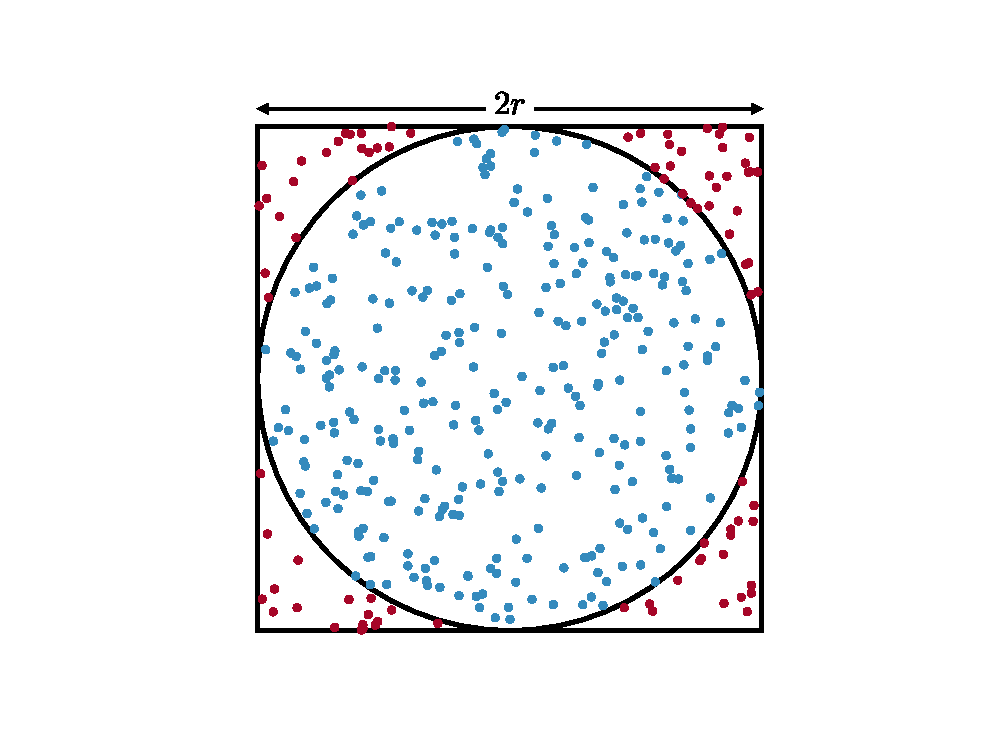
\includegraphics[scale=0.7]{../Images/montecarlointegration.eps}
	\caption{The value of $\pi$ can be estimated using Monte Carlo integration. Here we approximate the ratio between the area of a circle of radius $r$, $A_{\text{circle}}$, and the area of a square of side lengths $2r$, $A_{\text{square}}$, by counting the number of random points occurring inside the circle and inside the square. The estimate of $\pi$ is found from $\pi=4\cdot A_{\text{circle}}/A_{\text{square}}$.}
	\label{fig:montecarlointegration}
\end{figure}

Since we base this scientific work on solving equations numerically on the computer, software development is a significant part of the work. We will in this chapter go through the main concepts of scientific programming, and directly relate them to our code in the next chapters on implementation. As a motivation, we will provide a brief recap of some historical milestones in scientific computing.

Computers have long been used for solving complex scientific problems. Actually, for a long time, science was the primary motivation for developing computers. Already in 1929, Egil Hylleraas used his mechanical desk calculator to calculate the ground state energy of the helium atom, which remains a milestone in computational quantum chemistry as well as quantum chemistry in general \supercite{helgaker_perspective_2000}. Later, pioneers like Alan Turing and John von Neumann contributed to the invention of the first electronic computer, which made numerical solutions of ordinary differential equations possible \supercite{gustafsson_scientific_2018}. 

Also on the software side, big breakthroughs have been made since the advent of the electronic computer. The programming language Fortran was released in 1957, which provided a new basis of scientific programming \supercite{allen_history_1981}. Later, Ole Johan Dahl and Kristen Nygaard developed the language SIMULA, which is considered as the first object-oriented language \supercite{holmevik_compiling_1994}. The language that we mostly will rely on in this work, C++, is an extension of the language C which was developed in the early 1970s and is, together with Fortran, one of few languages that have survived the ravages of time. 

The computers used today, including both the hardware and the software, have become possible due to the heroic effort of an array of scientists, engineers, and mechanics over a long period. The computers are stronger than ever, have more memory than ever, are compacter than ever. Last but not least, they are more user-friendly than ever. All this has made heavy computations possible that were unthinkable just decades ago and has contributed to the development of virtually all branches of science. Due to the user-friendliness, advanced simulations have also been available for young and curious students like the author. We should not take this for granted. 

The computer's language itself is binary and is the lowest level. To translate commands to this language, we need a "translator", which is a language that fills the gap between the binary language and human commands. We categorize this language in levels based on how similar they are to the binary language. Low-level languages are more similar to the binary language than a high-level language, and the result is that low-level languages, in general, are more demanding to deal with, but they are typically faster than high-level languages. In our work, we use the low-level language C++ for the main code, but for scripting, including plotting and solving less expensive problems, the high-level language Python has been used. 

In this chapter, we will explain the essentials behind scientific programming, using examples from both C++ and Python. We will begin from the very basic, so if the reader is an experienced programmer, this chapter will probably be perceived as old news. Programs are often either classified as \textit{procedural programming} or \textit{object-oriented programming}, based on whether the code is written in the same order as the program flow goes (procedural) or is based on objects (object-oriented). We will explain the basics of object-oriented programming in the following.

\section{Object-oriented programming in Python}
In everyday life, we are all the time surrounded by objects that we categorize based on properties like their function, behavior, or expression. For instance, a \textit{circle} is an object with properties like area, circumference \textit{et cetera}, and can be categorized as a \textit{shape}. Other members of the shape class might be squares and triangles. In object-oriented programming, we create similar objects, or classes, to make the program flow more intuitive for the reader. The main class is called the parent class, while the sub-classes are called the children. The reason for this analogy is that the sub-classes always inherit from their main class, but not the other way around. The example with the shapes can therefore be implemented with \texttt{Shapes} being the parent, and \texttt{Circle}, \texttt{Square} and \texttt{Triangle} being its children. In the high-level language Python, this can be implemented in the following way:

\lstset{basicstyle=\scriptsize}
\begin{lstlisting}[language=python, caption={Geometric shapes implemented in object-oriented Python.}, label={lst:python}]
import numpy as np

class Shapes:
	def __init__(self, r):
		self.r = r

	def getArea(self):
		raise NotImplementedError("Class {} has no instance 'getArea'.".format(self.__class__.__name__))


class Circle(Shapes):
	def getArea(self):
		'''Returns the area of the circle. '''
		return np.pi*self.r**2

	def getCircumference(self):
		'''Returns the circumference of the circle. '''
		return 2*np.pi*self.r

	def contains(self, x, y):
		'''Returns True if the point (x,y) is inside the circle. '''
		if np.linalg.norm([x,y]) < self.r:
			return True
		return False

class Square(Shapes):
	def getArea(self):
		'''Returns the area of the square. '''
		return 4*self.r**2

	def getCircumference(self):
		'''Returns the circumference of the square. '''
		return 8*self.r

	def contains(self, x, y):
		'''Returns True if the point (x,y) is inside the square. '''
		if abs(x) < self.r and abs(y) < self.r:
			return True
	return False

class Triangle(Shapes):
	def getCircumference(self):
		'''Returns the circumference of the equilateral triangle. '''
		return 6*self.r
\end{lstlisting}
We give the children the properties area, circumference and extent. The length \texttt{r} means the radius of a circle, half the side length of a square and also half a side length of the equilateral triangle, as illustrated in figure \eqref{fig:montecarlointegration}. We can implement a circle, square and triangle of \texttt{r}=1, respectively named "circ", "squr" and "tria" by these three lines
\lstset{basicstyle=\scriptsize}
\begin{lstlisting}[language=python]
circ = Circle(1)
squr = Square(1)
tria = Triangle(1)
\end{lstlisting}
Moreover, we can easily get their areas by calling the \texttt{getArea()} function,
\lstset{basicstyle=\scriptsize}
\begin{lstlisting}
>>> circ.getArea()
3.141592653589793

>>> squr.getArea()
4

>>> tria.getArea()
NotImplementedError: Class Triangle has no instance 'getArea'.
\end{lstlisting}

As we can see, the area of the circle and the square were calculated successfully, giving $\pi r^2$ and $4r$ respectively. On the other hand, the area of the triangle raised an error, which is because we do not have defined the area of the triangle! This example illustrates that the properties of the children overwrites the properties of the parent, but if a child does not have the called property, it will instead return the parent's property. 

\subsection{An example based on Monte Carlo simulations}
Up to this point, we have talked a lot about Monte Carlo simulations without giving an illustrating example of what it is. Methods where we draw numbers randomly from a function to reveal properties of a function, are in general classified as Monte Carlo simulations and in that manner, the name might sound more complicated than it is. 

Suppose we did not know the value of $\pi$, what could we do to approximate its value? There are many ways to do this, where the most intuitive might be to measure the ratio between the diameter and the circumference in a circle. It is not possible to do this very accurate manually. A more accurate solution would be to use Monte Carlo simulations, where we, for instance, can take the starting point on the relation
\begin{empheq}[box={\mybluebox[5pt]}]{equation}
\pi=4\frac{\text{A}_{\text{circle}}}{\text{A}_{\text{square}}},
\end{empheq}
which is derived from the ratio between the area of a circle of radius $r$ and the area of a square of side lengths $2r$. By drawing random numbers from a uniform distribution and count the number of points that are in the square and the circle, we can approximate $\text{A}_{\text{circle}}/\text{A}_{\text{square}}$. We can do this by using the \texttt{getExtent()} function of the square class and circle class,
\lstset{basicstyle=\scriptsize}
\begin{lstlisting}[language=python]
for i in range(1,10):                      # Iteration loop
	M = 10**i
	A_square = 0
	A_circle = 0
	for _ in range(int(M)):                # Monte Carlo loop
		x = np.random.uniform(-1,1)
		y = np.random.uniform(-1,1)
		if circ.contains(x,y):
			A_circle += 1
		if squr.contains(x,y):
			A_square += 1
	print("MC = 10^", i, "Pi: ", 4 * A_circle/A_square)
\end{lstlisting}
which gives a output similar to
\begin{lstlisting}
MC = 10^1 Pi:  2.4
MC = 10^2 Pi:  3.32
MC = 10^3 Pi:  3.156
MC = 10^4 Pi:  3.1296
MC = 10^5 Pi:  3.14168
MC = 10^6 Pi:  3.140044
MC = 10^7 Pi:  3.1420708
MC = 10^8 Pi:  3.1416844
MC = 10^9 Pi:  3.141615628
\end{lstlisting}
Note that the value of $\pi$ was never used in this calculation. Considering the fact that $\pi=3.141592653589793...$, the obtained result is quite acceptable. However, to run the program with $M=10^9$ Monte Carlo cycles, the program is quite slow. Is it possible to do this faster? The answer is yes, by switching partly or entirely to a low-level language.

\section{Low-level programming with C++}
Above, we looked at how inheritance can be implemented in the high-level language Python, and we observed the main weakness of high-level languages: the computational time. In this section, we will repeat the implementation above using C++. Using a low-level language will, hopefully, provide a significant speed-up. A similar C++ class structure as the Python class presented listing \ref{lst:python} looks like
\lstset{basicstyle=\scriptsize}
\begin{lstlisting}[language=c++, caption={Geometric shapes implemented in object-oriented C++.}, label={lst:cpp}]
class Shapes {
	public:
		Shapes();
		virtual double getArea() = 0;
		virtual double getCircumference() = 0;
		virtual bool contains(double x, double y) = 0;
		virtual ~Shapes();
	private:
		double m_r;
};

class Circle : public Shapes {
	public:
		Circle(double r);
		double getArea() {
			/* Returns the area of the circle. */
			return M_PI * m_r * m_r;
		}
		double getCircumference() {
			/* Returns the circumference of the circle. */
			return 2 * M_PI * m_r;
		}
		bool contains(double x, double y) {
			/* Returns true if the point (x,y) is inside the circle. */
			if(sqrt(x*x+y*y) < m_r) {
				return true;
			}
			return false;
		}
};

Circle::Circle(double r) : Shapes() {
	m_r = r;
}

class Square: public Shapes {
	public:
		Square(double r);
		double getArea() {
			/* Returns the area of the square. */
			return 4 * m_r * m_r;
		}
		double getCircumference() {
			/* Returns the circumference of the square. */
			return 8 * m_r;
		}
		bool contains(double x, double y) {
			/* Returns true if the point (x,y) is inside the square. */
			if(fabs(x) < m_r && fabs(y) < m_r) {
				return true;
			}
			return false;
		}
};

Square::Square(double r) : Shapes() {
	m_r = r;
}
\end{lstlisting}
This looks different from the implementation in Python presented in listing \eqref{lst:python}. We will go thoroughly through the different parts of the code. One of the first thing we observe, is that we here need to \textit{declare} all the variables, meaning that we need to specify the variable type. In the following we will have a look at some standard \textit{data types}.

\subsection{Built-in data types}
In low-level languages, we need to specify the data types manually, enhancing the control. The most fundamental data types are \texttt{int} representing an integer number, \texttt{float} representing a floating number, \texttt{bool} representing a Boolean number and \texttt{char} representing a character. Often, these four data types are not sufficient for the task we want to implement, and we need to introduce more data types. An especially common error is \textit{overflow}, meaning that the number computed is out of the range of our data type. To avoid this, we can switch to data types of longer range, replacing \texttt{int} with a \texttt{long long int} (or just a \texttt{long long}), and replacing \texttt{float} with a \texttt{double}.

\begin{table}
	\caption{Built-in data types in C++, with their memory occupation and range in a 64-bit processor, taken from \supercite{noauthor_c++_2017}. Extensions in the parenthesis are optional.}
	\label{tab:datatypes}
	\begin{tabularx}{\textwidth}{R{0.5cm}L{7cm}R{1.5cm}R{5cm}R{0.3cm}} \hline\hline
		&\makecell{\\ Data types \\ \phantom{=}} & Size [bytes] & Range & \\ \hline \\
		&(\texttt{signed}) \texttt{char} & 1 & $-2^7$ to $2^{7}-1$ & \\ 
		&(\texttt{signed}) \texttt{short} (\texttt{int}) & 2 & $-2^{15}$ to $2^{15}-1$ & \\
		&(\texttt{signed}) \texttt{int} / \texttt{long} (\texttt{int}) & 4 & $-2^{31}$ to $2^{31}-1$ & \\ 
		&(\texttt{signed}) \texttt{long long} (\texttt{int}) & 8 & $-2^{63}$ to $2^{63}-1$ & \\ \\
		&\texttt{unsigned char} & 1 & 0 to $2^{8}$ & \\ 
		&\texttt{unsigned short} (\texttt{int}) & 2 & 0 to $2^{16}$ & \\
		&\texttt{unsigned int} / \texttt{unsigned long} (\texttt{int}) & 4 & 0 to $2^{32}$ & \\ 
		&\texttt{unsigned long long} (\texttt{int}) & 8 & 0 to $2^{64}$ & \\ \\
		&\texttt{float} & 4 & $\sim$ $\pm$3.4E38 ($\sim$ 7 digits) & \\
		&(\texttt{long}) \texttt{double} & 8 & $\sim$ $\pm$1.7E308 ($\sim$ 15 digits) & \\
		\hline\hline
	\end{tabularx}
\end{table} 

Some languages also deal with \texttt{long int} and \texttt{long double}, but in C++ an \texttt{int} and a \texttt{long int} is the same. Additionally, a \texttt{long double} is the same as a \texttt{double}. As lack of memory is typically not the largest problem when performing simulations, it is common to declare all floating numbers as \texttt{double}s. In table \eqref{tab:datatypes}, the most common data types are listed with their range and memory occupation in C++. For integers, it is also possible to "move" the range from its zero-centered default to only include positive numbers. This is done by declaring an \texttt{unsigned} data type. By using unsigned data types, the range doubles in the positive direction, but it should not be done if we, by any chance, can get negative numbers, as we then get \textit{underflow}.  

\subsection{Access modifiers}
Another thing that we observe from the code example in listing \eqref{lst:cpp}, is that we define the functions as \texttt{private} or \texttt{public}, which are called access modifiers. The access modifiers specify how much access the environment should have to the function: \texttt{private} means that the function can only be called from the particular class, while \texttt{public} means that also sub-classes (children) and other classes have access to the function. We also have a third access modifier in C++, called \texttt{protected}. \texttt{protected} members of a class A are not accessible outside of A's code, but any class that inherits from A has access to the protected member. 

\subsection{Virtual functions}
In the Python example in listing \eqref{lst:python}, we saw how a parent's function was overwritten by a function of the child. This works as long as the child's function has an identical name and identical arguments as the parent's function; otherwise it all will fail. In C++, a safer method exists based on virtual functions, where a child is \textit{forced} to have the same virtual functions as its parent. The virtual functions of the parent therefore serves as a template of its children, such that all the children have the same features. If the parent function is empty, the function is called pure virtual. This is often very useful, as the children tend to have the same features. Taking it back to the \texttt{Shapes} class, all the shapes ought to have features area and circumference, which can be forced by using virtual functions, as done in the example above, where all functions are pure virtual.

\subsection{Constructors and destructors}
In the C++ example in \eqref{lst:cpp}, we observe that the class \texttt{Shapes} has a function with the same name, \texttt{Shapes} and another virtual function $\sim$\texttt{Shapes}. The former one is used to create the object and is hence named a \textit{constructor}. This function is called automatically when the object of a class is created. Similarly, the latter one destructs an object when we are done evaluating the object. It is therefore named a \textit{destructor} and is also called automatically when an object is deleted or goes out of scope.

\subsection{Pointers}
In the C++ example in \eqref{lst:cpp}, we have not directly used any pointer. However, pointers are important in low-level languages, and we will here give a very brief introduction to pointers. For a C++ program, the memory of a computer is like a succession of memory cells, each with a unique address and of size one byte. When declaring a variable of size larger than one byte, the object will occupy memory cells that have consecutive addresses. Often, it is useful to know this address, which allows us to change the object directly in the memory. The address of a variable is given by the address-of operator, \&, working as
\lstset{basicstyle=\scriptsize}
\begin{lstlisting}[language=C++]
address=&variable
\end{lstlisting}
By doing this, we say that we \textit{point to the address}, and a variable that stores the address of another variable is thereby called a pointer. Furthermore, the dereference operator, *, gives the value of the address to where a pointer points. Thus, the following is true
\begin{lstlisting}[language=C++]
variable=*address
\end{lstlisting}

\subsection{Back to the Monte Carlo example}
We can now call the class above from the \texttt{main} function. We start defining the children \texttt{circ} and \texttt{squr}, and use the \texttt{contains()} function to approximate the area ratio between them. The code looks like 
\begin{lstlisting}[language=c++]
int main() {   
	class Shapes* circ = new Circle(1);
	class Shapes* squr = new Square(1);

	for(int i=1; i<10; i++) {
		int M = int(pow(10,i));
		long long A_square = 0;
		long long A_circle = 0;
		for(int m=0; i<M; i++) {
			double x = uniform(gen);
			double y = uniform(gen);
			if(circ->contains(x, y)) {
				A_circle ++;
			}
			if(squr->contains(x, y)) {
				A_square ++;
			}
		}
		std::cout << std::fixed;
		std::cout << std::setprecision(10);
		std::cout << "MC = 10^" << i << "Pi: " << 4 * double(A_circle)/A_square << std::endl;
	}
	return 0;
}
\end{lstlisting}
This gives a similar output as the Python script, but is much faster.

\iffalse
\subsection{Data types in Eigen}
The open source template library for linear algebra, Eigen, will be used throughout the coding, and it comes with arrays of various properties. The most relevant ones are \texttt{VectorXi}, which has dynamic length and \texttt{int} data type and \texttt{VectorXd}, which has dynamic length and \texttt{double} data type. The Matrix class has equivalent objects. 

In cases where we have \textit{a priori} knowledge of the array size, we can replace the \texttt{X} with the actual size. A fixed $3\times 3$ matrix of type \texttt{double} can for example be declared as \texttt{Matrix3d}. According to the Eigen documentation, using fixed size is \textit{"...hugely beneficial to performance"}. \url{https://eigen.tuxfamily.org/dox/group__TutorialMatrixClass.html}.
\fi
    \chapter{Implementation: Variational Monte Carlo} \label{chp:WFE}
\epigraph{There are only two hard things in Computer Science: cache invalidation and naming things.}{Phil Karlton, \cite{fowler_bliki:_nodate}}
\iffalse
\begin{figure}[H]
	\centering
	
\includegraphics[scale=0.4]{Images/example.png}
	\caption{Caption}
\end{figure}
\fi

In this chapter de will describe the implemented variational Monte Carlo (VMC) code, which was developed from scratch in C++. As the code itself is around 7000 significant\footnote{Significant lines of code in this sense means lines that are not blank or commented. Counted by the cloc program \cite{aldanial_cloc_2019}.} lines of code, we will just go through selected and often not obvious parts. As often said, \textit{good planning is half the battle}, which largely relates to writing VMC code. The code was rewritten and restructured several times before we ended on the final version. As a starting point, we used the VMC framework implemented by \citet{ledum_simple_2016}, which was meant as an example implementation in the course \textit{FYS4411 - Computational Physics II: Quantum Mechanical Systems}. The entire source code can be found on the authors GitHub account, \url{github.com/evenmn/VMC}.

The code was developed with focus on three main goals: it should be efficient, flexible and readable. It needs to be flexible in order to support the Boltzmann machines as our trial wave function guess, and since we will try out various Jastrow factors it should be easy to add and remove wave function elements. Since quantum mechanical simulations in general are very expensive, it is important to develop efficient code to be able to study systems of some size. Lastly, we aim to write readable code such that others can reuse the code in its entirety or parts of it later.  How we work to achieve the goals will be illustrated by code mainly picked from the \lstinline{WaveFunction} class, which is the heart of the code.

For all matrix operations, the open source template library for linear algebra Eigen was used throughout the code. Eigen provides an elegant interface, with support for all the needed matrix and vector operations. In addition, Eigen is built on the standard software libraries for numerical linear algebra, BLAS and LAPACK, which are incredibly fast. These contribute greatly to the performance of the code. 

\section{Flexibility and readability}
We have done several things in order to keep the code as readable as possible. Firstly, the code was written in an object orientated scheme which makes it more intuitive to a human as discussed in chapter \ref{chp:scientificprogramming}. Actually, the Hamiltonians, optimizers, wave functions, sampling methods and even the random number generator were treated as objects, making the code more or less as object orientated as possible. This makes it also easier to define a system, since we simply can set the preferred object. Below, we define a two-dimensional quantum dot system of 6 electrons with frequency $\omega=1.0$, learning rate $\eta=0.1$, number of Metropolis cycles $M=2^{20}=1048576$ and max number of iterations set to 1000.

\begin{lstlisting}[language={C++}, caption={Example on how a quantum dot system can be initialized.}, label={lst:qd}]
System *QD = new System();

QD->setNumberOfDimensions(2);
QD->setNumberOfParticles(6);
QD->setNumberOfMetropolisSteps(int(pow(2, 20)));
QD->setFrequency(1.0);
QD->setLearningRate(0.1);

QD->setBasis(new Hermite(QD));
QD->setHamiltonian(new HarmonicOscillator(QD));

QD->setWaveFunctionElement(new Gaussian(QD));
QD->setWaveFunctionElement(new SlaterDeterminant(QD));
QD->setWaveFunctionElement(new PadeJastrow(QD));

QD->runIterations(1000);
\end{lstlisting}
We observe that one first needs to define an object to represent the system, and then the various settings can be connected to this object. As you might notice, we use the \textbf{lowerCamelCase} naming convention for function and variable names, which means that each word begins with a capital letter except the initial word. For classes, we use the \textbf{UpperCamelCase} to distinguish from function names. This is known to be easy to read, and apart from for example the popular \textbf{snake\_case}, we do not need delimiters between the words, which saves some space. After the naming convention is decided, we are still responsible for giving reasonable names, which is not always an easy task, as Karlton points out. When one sees the name, one should know exactly what the variable/function/class is or does. In addition, as a code format we use the ClangFormat, which provides a consequent way of formatting the code. 

The snippet above also demonstrates how the code is made flexible when it comes to the wave function. One can simply construct a wave function consisting of various elements by calling the \lstinline{setWaveFunctionElement} multiple times. This creates a wave function vector, \lstinline{m_waveFunctionVector}, in the background containing all the elements, which makes it easy to compose the wave function in whatever way you want, all the elements can be combined. The reader might stubs on the use of the element \lstinline{Gaussian}, isn't the trial wave function defined by the Slater determinant multiplied with a Padé-Jastrow factor? It is, but as we will see later in section \ref{sec:factorizing}, the Gaussian part can be factorized out of the Slater determinant when using a Hermite basis. However, we will now start from the fundamental assumption that the trial wave function consists of a Slater determinant and a Jastrow factor, and take it from there. 

\section{Splitting the wave function in elements}
In a standard VMC calculation, the trial wave function, $\Psi_T(\bs{r})$, is assumed to consist of a single Slater determinant and a Jastrow factor to take care of the repulsive interactions. Mathematically it can be expressed as
\begin{equation}
\Psi_T(\bs{r})=|\hat{D}(\bs{r})|J(\bs{r}_{ij})
\end{equation}
where $\bs{r}$ is the set of coordinates of all the particles and $\bs{r}_{ij}$ are the distances between all the particles. $J(\bs{r}_{ij})$ is an arbitrary Jastrow factor, while the Slater determinant is the determinant of the matrix $\hat{D}(\bs{r})$, henceforth the Slater matrix. To convince the reader that the Slater determinant and the Jastrow factor can be treated separately, we will consider a general trial wave function consisting of $p$ wave function elements $\{\Psi_1, \Psi_2\hdots\Psi_p\}$,
\begin{empheq}[box={\mybluebox[5pt]}]{equation}
\Psi_T(\bs{r}) = \prod_{i=1}^p\Psi_i(\bs{r}),
\label{eq:elementproduct}
\end{empheq}
where $\Psi_i(\bs{r})$ in principle can be any function of the coordinates $\bs{r}$. However, we will later see that the parameter update simplifies if we restrict each variational parameter $\theta_j$ to appear in an element only. Before that, we will look at how the kinetic energy can be expressed in terms of independent factors.

\subsection{Kinetic energy computations} \label{sec:kinetic}
The local energy computation is the heart of the VMC code, and the aim for an efficient and flexible code starts here. It was first defined in equation \eqref{eq:localenergy}, and by inserting a general Hamiltonian $\hat{\mathcal{H}}=-1/2\nabla^2+V$ with $V$ covering all the potential energy, we obtain
\begin{equation}
E_L=\sum_{k=1}^F\Big[-\frac{1}{2}\Big(\frac{1}{\Psi_T(\bs{r})}\nabla_k^2\Psi_T(\bs{r})\Big) + V\Big],
\end{equation}
where we have $F=ND$ degrees of freedom. As always, $N$ is the number of particles and $D$ is the number of dimensions. The first term, which is the kinetic energy term, is the only wave function-dependent one, and we will in this section split it up with respect to the elements. The potential energy term, $V$, is not directly dependent on the wave function and will therefore not be further touched here. 

From the definition of the derivative of a logarithm, we have that
\begin{equation}
\frac{1}{\Psi_T(\bs{r})}\nabla_k\Psi_T(\bs{r})=\nabla_k\ln\Psi_T(\bs{r}),
\label{eq:derlogdef}
\end{equation}
which can be used to prove the following relation 
\begin{equation}
\frac{1}{\Psi_T(\bs{r})}\nabla_k^2\Psi_T(\bs{r})=\nabla_k^2\ln\Psi_T(\bs{r}) + (\nabla_k\ln\Psi_T(\bs{r}))^2.
\label{eq:secderlogdef}
\end{equation}
Expressing the kinetic energy in terms of this relation is useful because most of the elements can be treated easily in the log-space. By using the fact that the trial wave function is a product of all the elements, the term above is calculated by
\begin{equation}
\frac{1}{\Psi_T(\bs{r})}\nabla_k^2\Psi_T(\bs{r})=\sum_{i=1}^p\nabla_k^2\ln\Psi_i(\bs{r}) + \Big(\sum_{i=1}^p\nabla_k\ln\Psi_i(\bs{r})\Big)^2
\end{equation}
such that the total kinetic energy is given by
\begin{empheq}[box={\mybluebox[5pt]}]{equation}
-\frac{1}{2}\frac{1}{\Psi_T(\bs{r})}\nabla^2\Psi_T(\bs{r})=-\frac{1}{2}\bigg[\sum_{i=1}^p\nabla^2\ln\Psi_i(\bs{r}) + \sum_{k=1}^{F}\Big(\sum_{i=1}^p\nabla_k\ln\Psi_i(\bs{r})\Big)^2\bigg].
\label{eq:splittedkineticenergy}
\end{empheq}
This can be found when all local derivatives $\nabla^2\ln\Psi_i(\bs{r})$ and $\nabla_k\ln\Psi_i(\bs{r})$ are given. By assuming that the former is returned by a function \lstinline{computeLaplacian()} and the latter is returned by a function \lstinline{computeGradient(k)}, we compute the kinetic energy using the following function
\lstset{basicstyle=\scriptsize}
\begin{lstlisting}[language=c++]
double System::getKineticEnergy()
{
	double kineticEnergy = 0;
	for (auto &i : m_waveFunctionElements) {
		kineticEnergy += i->computeLaplacian();
	}
	for (int k = 0; k < m_degreesOfFreedom; k++) {
		double nablaLnPsi = 0;
		for (auto &i : m_waveFunctionElements) {
			nablaLnPsi += i->computeGradient(k);
		}
		kineticEnergy += nablaLnPsi * nablaLnPsi;
	}
	return -0.5 * kineticEnergy;
}
\end{lstlisting}
Note that some of the variables are declared globally, here the vector \lstinline{m_waveFunctionElements} and the integer \lstinline{m_degreesOfFreedom} are denoted by an \lstinline{m_} to distinguish them from the variables declared locally. 

\subsection{Parameter gradients}
In section \ref{sec:parameterupdate}, we presented how the parameters can be updated by minimizing the energy expectation value. We recall that the only closed-form expression needed in addition to the local energy is $\nabla_{\theta_j}\ln\Psi_T(\bs{r}_i)$, which needs to be found. By applying equation \eqref{eq:elementproduct}, we find that
\begin{empheq}[box={\mybluebox[5pt]}]{equation}
\nabla_{\theta_j}\ln\Psi_T(\bs{r})=\sum_{i=1}^p\nabla_{\theta_j}\ln\Psi_i(\bs{r})=\nabla_{\theta_j}\ln\Psi_{\theta_j}(\bs{r}),
\end{empheq}
where $\Psi_{\theta_j}(\bs{r})$ is the only element which contains the parameter $\theta_j$. With this in mind, we need to find closed-form expressions of $\nabla_{\theta_j}\ln\Psi_{\theta_j}(\bs{r})$ for all wave function elements $\Psi_{\theta_j}(\bs{r})$ that are associated with a variational parameter $\theta_{j}$.

In the code, we store all the parameters in a \textit{parameter matrix} where each element has its own row of parameters. Similarly, we create a \textit{gradient matrix} of the same dimensions to store the gradients $\nabla_{\theta_j}\ln\Psi_{\theta_j}(\bs{r})$ for each variational parameter. The function which collect all the gradients is implemented straight-forwardly, and is given by
\begin{lstlisting}[language=c++]
Eigen::MatrixXd System::getAllParameterGradients()
{
	for (int i = 0; i < m_numberOfElements; i++) {
		m_gradients.row(i) = m_waveFunctionElements[i]->computeParameterGradient();
	}
	return m_gradients;
}
\end{lstlisting}
where \lstinline{m_gradients} has the same number of rows as the number of elements and the same number of columns as the maximum number of parameters in an element $i$. The function \lstinline{computeParameterGradient()} returns a vector with all the gradients $\nabla_{\theta_j}\ln\Psi_i(\bs{r})$ of the respective element. Even though the gradients are used to update the parameters, we will postpone the discussion of the parameter update to section \ref{sec:update}.

\subsection{Probability ratio} \label{sec:probabilityratio}
In the two previous sections, we have seen how the derivatives of the wave function elements can be used in order to obtain the local energy and the parameter update. However, we also need the evaluation of the wave function elements themselves to decide whether or not a move should be accepted. If we go back to equation \eqref{eq:acceptance}, we see that what is actually needed is the ratio between the present and the previous probability, $P(\bs{r}_{\text{new}})/P(\bs{r}_{\text{old}})$. Further, we can write this as the product of the probability ratios of all the wave function elements, 
\begin{empheq}[box={\mybluebox[5pt]}]{equation}
\frac{P(\bs{r}_{\text{new}})}{P(\bs{r}_{\text{old}})}=\frac{|\Psi_T(\bs{r}_{\text{new}})|^2}{|\Psi_T(\bs{r}_{\text{old}})|^2}=\prod_{i=1}^p\frac{|\Psi_i(\bs{r}_{\text{new}})|^2}{|\Psi_i(\bs{r}_{\text{old}})|^2},
\end{empheq}
again utilizing equation \eqref{eq:elementproduct}. Finding closed-form expressions for those ratios is not only beneficial because it is needed in the actual implementation, as we work in the log-space those ratios often take clean forms which are cheap to evaluate. Below, we will calculate those ratios for all the elements since we are going to use that directly in the sampling. We name the function returning the ratio for a particular element \lstinline{evaluateRatio()}, and we obtain the total probability ratio in the following way
\begin{lstlisting}[language=c++]
double System::evaluateProbabilityRatio()
{
	double ratio = 1;
	for (auto &i : m_waveFunctionElements) {
		ratio *= i->evaluateRatio();
	}
	return ratio;
}
\end{lstlisting}

With this, we have introduced the four central functions of the wave function elements: \lstinline{computeLaplacian()}, \lstinline{computeGradient(k)}, \lstinline{computeParameterGradient()} and \lstinline{evaluateRatio()}. In the following, we will evaluate the Slater determinant and see how it can be split further in more elements. 

\section{Slater determinant}
As we have seen above, the Slater determinant is the fundamental part of the trial wave function, together with the Jastrow factor. The main problem with the Slater determinant, is that it is very expensive to deal with as the number of particles increases. To find the gradient of the Slater determinant, as requested by equation \eqref{eq:splittedkineticenergy}, we need to compute the inverse of the Slater matrix, which by standard LU decomposition scales as $\sim N^3$ for an $N\times N$ matrix \cite{trahan_computational_2006}. Fortunately, there exist algorithms that let us obtain the inverse of the matrix by recursive relations, scaling as $\sim N^2$. This will be detailed in section \ref{sec:efficientcalculationsofslaterdeterminant}.

Additionally, the Slater determinant can be split in a spin-up part and a spin-down part, which reduces the Slater matrix to two $N/2\times N/2$ matrices. Also factorizing out common functions from the Slater determinant will give some speed-up. In this section, we will mostly discuss the various methods to make the update of the Slater matrix more efficient. Before we proceed further, we will reintroduce the Slater determinant from section \ref{sec:slater},
\begin{equation}
\Psi_{sd}(\bs{r},\bs{\sigma})=|\hat{D}(\bs{r},\bs{\sigma})|\propto
\begin{vmatrix}
\phi_1(\boldsymbol{r}_1,\sigma_1) & \phi_2(\boldsymbol{r}_1,\sigma_2) & \hdots & \phi_N(\boldsymbol{r}_1,\sigma_N)\\
\phi_1(\boldsymbol{r}_2,\sigma_1) & \phi_2(\boldsymbol{r}_2,\sigma_2) & \hdots & \phi_N(\boldsymbol{r}_2,\sigma_N)\\
\vdots & \vdots & \ddots & \vdots \\
\phi_1(\boldsymbol{r}_N,\sigma_1) & \phi_2(\boldsymbol{r}_N,\sigma_2) & \hdots & \phi_N(\boldsymbol{r}_N,\sigma_N),
\end{vmatrix}
\label{eq:generalslater}
\end{equation}
as it is the starting point of our optimizations. We also recall that $\sigma_i$ is the spin and $\phi_j(\bs{r}_i,\sigma_j)$ is the single-particle function occupying the matrix element $D_{ij}$.

\subsection{Splitting up the Slater determinant} \label{sec:splittingofslater}
In order to reduce the computational cost of the Slater determinant, we will split it up in a spin-up part and a spin-down part. The splitting was explained thoroughly by Daniel Nissenbaum in his doctoral dissertation, appendix I in \cite{nissenbaum_stochastic_2008}, and this section is heavily inspired by it. In real life, we cannot immediately tell if an electron has spin-up or spin-down, but since we in the code need to know which particles that have spin-up and spin-down, we simply decide that the first $N_{\uparrow}$ particles have spin up and the remaining particles have spin down. 

In addition to reduce the computational cost, splitting up the Slater determinant also makes it possible to factorize out the spin-part from the single-particle functions. Only the spatial part of the single particle functions contribute to the energies, such that we with advantage can get rid of the spin parts. Recall that the single-particle functions $\psi(\bs{r},\sigma)$, can be written as a tensor product between the spatial part $\phi(\bs{r})$ and the spin part $\xi(\sigma)$, 
\begin{equation}
\psi(\bs{r},\sigma)=\phi(\bs{r})\otimes\xi(\sigma) 
\end{equation}
where only the spatial part is dependent on the coordinates. As we in the ground state have double degeneracy, the spatial part will be the same for pairwise spin-up and spin-down particles, and we arrange them as
\begin{equation}
\psi_j(\bs{r}_i,\sigma_i)=
\begin{cases}
\phi_j(\bs{r}_i)\xi_{\uparrow}(\sigma_i)\quad\quad&\text{if } j<N_{\uparrow}\\
\phi_j(\bs{r}_i)\xi_{\downarrow}(\sigma_i)\quad\quad&\text{if } j\geq N_{\uparrow}.
\end{cases}
\end{equation}
Since the first $N_{\uparrow}$ particles have spin up, $\sigma_i=\,\uparrow\quad\forall\quad i\in\{1,2,...,N_{\uparrow}\}$, and the remaining have spin down, we can now set up the Slater determinant in equation \eqref{eq:generalslater} where each single particle function is split in a spatial part and a spin part,
\begin{equation*}
\Psi_{sd}(\boldsymbol{r},\bs{\sigma})\propto
\begin{vmatrix}
\phi_1(\boldsymbol{r}_1)\xi_{\uparrow}(\uparrow) & \hdots & \phi_{N_{\uparrow}}(\boldsymbol{r}_1)\xi_{\uparrow}(\uparrow) & \phi_{1}(\boldsymbol{r}_1)\xi_{\downarrow}(\uparrow) & \hdots & \phi_{N_{\downarrow}}(\boldsymbol{r}_1)\xi_{\downarrow}(\uparrow)\\
\vdots & & \vdots & \vdots & & \vdots \\
\phi_1(\boldsymbol{r}_{N_{\uparrow}})\xi_{\uparrow}(\uparrow) & \hdots & \phi_{N_{\uparrow}}(\boldsymbol{r}_{N_{\uparrow}})\xi_{\uparrow}(\uparrow) & \phi_{1}(\boldsymbol{r}_{N_{\uparrow}})\xi_{\downarrow}(\uparrow) & \hdots & \phi_{N_{\downarrow}}(\boldsymbol{r}_{N_{\uparrow}})\xi_{\downarrow}(\uparrow)\\
\phi_1(\boldsymbol{r}_{N_{\uparrow}+1})\xi_{\uparrow}(\downarrow) & \hdots & \phi_{N_{\uparrow}}(\boldsymbol{r}_{N_{\uparrow}+1})\xi_{\uparrow}(\downarrow) & \phi_{1}(\boldsymbol{r}_{N_{\uparrow}+1})\xi_{\downarrow}(\downarrow) & \hdots & \phi_{N_{\downarrow}}(\boldsymbol{r}_{N_{\uparrow}+1})\xi_{\downarrow}(\downarrow)\\
\vdots & & \vdots & \vdots & & \vdots \\
\phi_1(\boldsymbol{r}_N)\xi_{\uparrow}(\downarrow) & \hdots & \phi_{N_{\uparrow}}(\boldsymbol{r}_N)\xi_{\uparrow}(\downarrow) & \phi_{1}(\boldsymbol{r}_N)\xi_{\downarrow}(\downarrow) & \hdots & \phi_{N_{\downarrow}}(\boldsymbol{r}_N)\xi_{\downarrow}(\downarrow)\\
\end{vmatrix}.
\end{equation*}
We observe that the the spin-up particles sometimes occupy spin-down states, which they are not allowed to. Therefore, half of the elements become zero and the determinant can be further expressed as
\begin{equation*}
\Psi_{sd}(\boldsymbol{r},\bs{\sigma})\propto
\begin{vmatrix}
\phi_1(\boldsymbol{r}_1)\xi_{\uparrow}(\uparrow) & \hdots & \phi_{N_{\uparrow}}(\boldsymbol{r}_1)\xi_{\uparrow}(\uparrow) & 0 & \hdots & 0\\
\vdots & & \vdots & \vdots & & \vdots \\
\phi_1(\boldsymbol{r}_{N_{\uparrow}})\xi_{\uparrow}(\uparrow) & \hdots & \phi_{N_{\uparrow}}(\boldsymbol{r}_{N_{\uparrow}})\xi_{\uparrow}(\uparrow) & 0 & \hdots & 0\\
0 & \hdots & 0 & \phi_{1}(\boldsymbol{r}_{N_{\uparrow}+1})\xi_{\downarrow}(\downarrow) & \hdots & \phi_{N_{\downarrow}}(\boldsymbol{r}_{N_{\uparrow}+1})\xi_{\downarrow}(\downarrow)\\
\vdots & & \vdots & \vdots & & \vdots \\
0 & \hdots & 0 & \phi_{1}(\boldsymbol{r}_N)\xi_{\downarrow}(\downarrow) & \hdots & \phi_{N_{\downarrow}}(\boldsymbol{r}_N)\xi_{\downarrow}(\downarrow)\\
\end{vmatrix}
\end{equation*}
where the Slater matrix now is block diagonal! For a general block diagonal matrix, the determinant is given by the product of the determinant of each block
\begin{equation}
\Psi_{sd}(\boldsymbol{r},\bs{\sigma})\propto|\hat{D}_{\uparrow}(\bs{r}_{\uparrow},\sigma_{\uparrow})|\cdot |\hat{D}_{\downarrow}(\bs{r}_{\downarrow},\sigma_{\downarrow})|
\end{equation}
which can be seen by writing the total matrix as a product over all the block diagonal matrix. $\hat{D}_{\uparrow}$ is the matrix containing all spin-up states and $\hat{D}_{\downarrow}$ is the matrix containing all spin-down states. Since all elements in the respective matrices contain the same spin function, it can be factorized out,
\begin{equation}
\Psi_{sd}(\boldsymbol{r},\bs{\sigma})\propto|\hat{D}_{\uparrow}(\bs{r}_{\uparrow})|\{\xi_{\uparrow}(\sigma_1^{\uparrow})\xi_{\uparrow}(\sigma_2^{\uparrow})\hdots\xi_{\uparrow}(\sigma_{N_{\uparrow}}^{\uparrow})\}\cdot |\hat{D}_{\downarrow}(\bs{r}_{\downarrow})|\{\xi_{\downarrow}(\sigma_{N_{\uparrow+1}}^{\downarrow})\hdots\xi_{\downarrow}(\sigma_{N-1}^{\downarrow})\xi_{\downarrow}(\sigma_{N}^{\downarrow})\}
\end{equation}
and omitted in the future study. We are then left with the Slater determinant
\begin{empheq}[box={\mybluebox[5pt]}]{equation}
\Psi_{sd}(\boldsymbol{r})\propto|\hat{D}_{\uparrow}(\bs{r}_{\uparrow})|\cdot |\hat{D}_{\downarrow}(\bs{r}_{\downarrow})|
\end{empheq}
which is independent of spin, i.e, the matrices now consist of the spatial functions $\phi_j(\bs{r}_i)$ as the elements. 

It is also worth to notice that the size of the spin-up matrix is determined by the number of spin-up particles, and it is similar for the spin-down matrix. This means that the we can change the total spin $S$ by adjusting the relative sizes of the determinants. In the implementation, however, we stick to the magic quantum numbers, where $N_{\uparrow}=N_{\downarrow}$. Otherwise, we get a spin dependent contribution in the Hamiltonian.

\subsection{Factorizing out elements} \label{sec:factorizing}
We have now seen how the Slater determinant can be split up in a spin-up part and a spin-down part. Before we evaluate these determinants, we should try to make the elements of the Slater matrices as simple as possible to save computational time. If all the elements have the same factor, the computations will get much cheaper if the factor is factorized out of the matrix. How this is possible can easiest be seen if we express the Slater determinant on a summation form,
\begin{equation}
\Psi_{sd}(\bs{r})\propto\sum_{q}(-1)^q\hat{P}\phi_1(\bs{r}_1)\phi_2(\bs{r}_2)\hdots\phi_N(\bs{r}_N),
\label{eq:slatersum}
\end{equation}
where the sum runs over all the possible permutations and $\hat{P}$ is the permutation operator, permuting coordinates pairwise. If all the (spatial) single particle functions $\phi_j(\bs{r}_i)$ can be split in two functions $f_j(\bs{r}_i)$ and $g(\bs{r}_i)$ where the latter is common for all the single particle functions,
\begin{equation}
\phi_j(\bs{r}_i)=f_j(\bs{r}_i)g(\bs{r}_i)
\end{equation}
the Slater determinant can be rewritten as
\begin{equation}
\begin{aligned}
\Psi_{sd}(\bs{r})&\propto\sum_{p}(-1)^p\hat{P}f_1(\bs{r}_1)g(\bs{r}_1)f_2(\bs{r}_2)g(\bs{r}_2)\hdots f_N(\bs{r}_N)g(\bs{r}_N)\\
&=g(\bs{r}_1)g(\bs{r}_2)\hdots g(\bs{r}_N)\sum_{p}(-1)^p\hat{P}f_1(\bs{r}_1)f_2(\bs{r}_2)\hdots f_N(\bs{r}_N)\\
&=\prod_{i=1}^Ng(\bs{r}_i)
\begin{vmatrix}
f_1(\boldsymbol{r}_1) & f_2(\boldsymbol{r}_1) & \hdots & f_N(\boldsymbol{r}_1)\\
f_1(\boldsymbol{r}_2) & f_2(\boldsymbol{r}_2) & \hdots & f_N(\boldsymbol{r}_2)\\
\vdots & \vdots & \ddots & \vdots \\
f_1(\boldsymbol{r}_N) & f_2(\boldsymbol{r}_N) & \hdots & f_N(\boldsymbol{r}_N)
\end{vmatrix}.
\end{aligned}
\end{equation}
This is very useful when dealing with some common basises. For instance, the Hermite basis is given by 
\begin{equation}
\phi_j(\bs{r}_i)\propto H_j(\bs{r}_i)\exp(-\frac{1}{2}\omega|\bs{r}_i|^2)
\end{equation}
where $H_j(\bs{r}_i)$ are the Hermite polynomials and the Gaussian part fulfills the requirement of $g(\bs{r}_i)$. Therefore, we can construct a Slater determinant containing the Hermite polynomials only, treating the Gaussian as an independent element. This is not only preferable from an efficiency point of view, by doing this the variational parameter in the Gaussian is also removed from the determinant, which means that we can implement the determinant without worrying about the variational parameters. With this in mind, we will first treat the Gaussian element, obtaining its derivative and optimization schemes. Moreover, in section \ref{sec:slaterdeterminant} we will discuss how the determinant can be treated efficiently. 

\subsection{Gaussian} \label{sec:simplegaussian}
When factorizing out the Gaussian part from the Slater determinant, we obtain the element
\begin{equation}
\Psi_{sg}(\bs{r}; \alpha)=\prod_{j=1}^Ng(\bs{r}_j)=\exp\Big(-\frac{1}{2}\omega\alpha\sum_{j=1}^Nr_j^2\Big)=\exp\Big(-\frac{1}{2}\omega\alpha\sum_{j=1}^{F}x_j^2\Big),
\end{equation}
with $N$ as number of particles, $D$ as the number of dimensions and $F=ND$ as the degrees of freedom. $\omega$ is the oscillator strength and $\alpha$ is a variational parameter, which for non-interacting atoms is 1. Because of the presence of $r_i^2$ the function can easily be treated both in Cartesian and spherical coordinates, but in this thesis we will focus on the former. We now use $j$ as our summation index, and reserve $i$ for the moved particle and $k$ as our the differentiating index. When changing a coordinate $x_i$ from $x_i^{\text{old}}$ to $x_i^{\text{new}}$, the probability ratio can easily be found to be 
\begin{empheq}[box={\mybluebox[5pt]}]{equation}
\label{eq:simplegaussianprobabilityratio}
\frac{|\Psi_{sg}(\bs{x}_{\text{new}})|^2}{|\Psi_{sg}(\bs{x}_{\text{old}})|^2}=\exp\Big(\omega\alpha\big((x_{i}^{\text{old}})^2-(x_{i}^{\text{new}})^2\big)\Big),
\end{empheq}
which is pretty cheap to evaluate. The gradient of $\ln\Psi_{sg}$ with respect to the coordinate $x_k$ is
\begin{empheq}[box={\mybluebox[5pt]}]{equation}
\nabla_k\ln\Psi_{sg}=-\omega\alpha x_k,
\end{empheq}
and the corresponding Laplacian is
\begin{empheq}[box={\mybluebox[5pt]}]{equation}
\nabla^2\ln\Psi_{sg}=-\omega\alpha F.
\end{empheq}
We observe that the factor $\omega\alpha$ is found in all the expressions above and only needs to be calculated again when the parameter $\alpha$ is updated, which is updated according to
\begin{empheq}[box={\mybluebox[5pt]}]{equation}
\nabla_{\alpha}\ln\Psi_{sg} = -\frac{1}{2}\omega\sum_{j=1}^Fx_j^2.
\end{empheq}
The implementation is very straight-forward, and looks like
\begin{lstlisting}[language=c++]
double Gaussian::evaluateRatio()
{
	return m_probabilityRatio;
}

double Gaussian::computeGradient(const int k)
{
	return -m_omegalpha * m_positions(k);
}

double Gaussian::computeLaplacian()
{
	return -m_omegalpha * m_degreesOfFreedom;
}

Eigen::VectorXd Gaussian::computeParameterGradient()
{
	m_gradients(0) = -0.5 * m_omega * m_positions.cwiseAbs2().sum();
	return m_gradients;
}
\end{lstlisting}
where \lstinline|m_omegalpha| is $\omega\alpha$. The probability ratio is calculated using
\begin{lstlisting}[language=c++]
double void Gaussian::updateProbabilityRatio(int changedCoord)
{
	m_probabilityRatio = exp(m_omegalpha * (m_positionsOld(changedCoord) * m_positionsOld(changedCoord) - m_positions(changedCoord) * m_positions(changedCoord)));
}
\end{lstlisting}
We see that matrix-vector operations are used when it is possible, which makes the computations very fast.

\iffalse
\subsection{Hydrogen-like orbitals} \label{sec:hydrogenlike}
The Hydrogen-like orbitals were presented in \eqref{eq:hydrogenlike}, but as we discussed earlier they cause some problems for atoms of the size of Neon and larger due to complex numbers. Instead, we decided to look at hydrogen-like orbitals with solid harmonics. Even though they do not have problems with complex numbers, they are quite complicated to differentiate, and the closed form will therefore be found by symbolic differentiating on the computer. However, we will do the exercise for the simplest case, which is sufficient for finding the Hydrogen and Helium ground states. This reads
\begin{equation}
\Psi_{hl}( \bs{r};\alpha)=\exp\Big(-Z\alpha\sum_{j=1}^Nr_j\Big)
\end{equation}
where $r_j$ is the distance from particle $j$ to the center. We then differentiate with respect to coordinate $x_k$, and obtain
\begin{equation}
\nabla_k\ln\Psi_{hl}=-Z\alpha\frac{x_k}{r_{k'}}
\end{equation}
The Laplacian is then given by
\begin{equation}
\nabla_k^2\ln\Psi_{hl}=-Z\alpha\Big(1-\frac{x_k^2}{r_{k'}^2}\Big)\frac{1}{r_{k'}}
\end{equation}
and the differentiation with respect to the variational parameter $\alpha$ is
\begin{equation}
\partial_{\alpha}\ln\Psi_{\text{hl}}=-Z\sum_{j=1}^Nr_j.
\end{equation}

For close-form expressions for higher order wave functions, please run the script \lstinline{generateHydrogenOrbitals.py}.
\fi

\subsection{The determinant} \label{sec:slaterdeterminant}
As discussed in section \ref{sec:splittingofslater}, the Slater determinant can be split in a spin-up part and a spin-down part, and further the common functions can be factorized out as shown in section \ref{sec:factorizing}. This means that the remaining determinant is not the full Slater determinant, and to distinguish it from the real Slater determinant, $\Psi_{sd}(\bs{r})$, we will denote the element by $det$, $\Psi_{det}(\bs{r})$. This determinant can of course still be splitted like the Slater determinant, 
\begin{equation}
\Psi_{det}(\bs{r})=
|\hat{D}_{\uparrow}(\bs{r}_{\uparrow})|\cdot |\hat{D}_{\downarrow}(\bs{r}_{\downarrow})|,
\end{equation}
where $r_{\uparrow}$ are the coordinates of particles with spin up (defined as the first $N_{\uparrow}$ coordinates) and $r_{\downarrow}$ are the coordinates of particles with spin down (defined as the last $N_{\downarrow}$ coordinates). 

We can now exploit the logarithmic scale, by using that the logarithm of a product corresponds to summarize the logarithm of each factor,
\begin{equation}
\ln\Psi_{det}=\ln|\hat{D}_{\uparrow}(\bs{r}_{\uparrow})|+\ln|\hat{D}_{\downarrow}(\bs{r}_{\downarrow})|
\end{equation}
such that we only need to care about one of the determinants when differentiating, dependent on whether the coordinate we differentiate with respect to is among the spin-up or the spin-down coordinates,
\begin{equation}
\nabla_k\ln\Psi_{det}=
\begin{cases} 
\nabla_k\ln|\hat{D}_{\uparrow}(\bs{r}_{\uparrow})| & \text{if} \quad k<N_{\uparrow}\\
\nabla_k\ln|\hat{D}_{\downarrow}(\bs{r}_{\downarrow})| & \text{if} \quad k\geq N_{\uparrow}.
\end{cases}
\end{equation}
Before we go further, we will introduce a more general notation which covers both the cases:
\begin{equation}
\hat{D}(\bs{r})\equiv \hat{D}_{\sigma}(\bs{r}_{\sigma})
\end{equation}
where $\sigma$ is the spin projection. When summarizing, the sum is always over all relevant coordinates. Furthermore, we have that
\begin{equation}
\nabla_k\ln|\hat{D}(\bs{r})|=\frac{\nabla_k|\hat{D}(\bs{r})|}{|\hat{D}(\bs{r})|}
\end{equation}
and
\begin{equation}
\nabla_k^2\ln|\hat{D}(\bs{r})|=\frac{\nabla_k^2|\hat{D}(\bs{r})|}{|\hat{D}(\bs{r})|}-\bigg(\frac{\nabla_k|\hat{D}(\bs{r})|}{|\hat{D}(\bs{r})|}\bigg)^2
\end{equation}
which are consistent with the equations \eqref{eq:derlogdef} and \eqref{eq:secderlogdef}. At this point, there are (at least) two possible paths to the final expressions. We can keep on using matrix operations and find the expressions of $\nabla_k|\hat{D}(\bs{r})|/|\hat{D}(\bs{r})|$ and $\nabla_k^2|\hat{D}(\bs{r})|/|\hat{D}(\bs{r})|$ using Jacobi's formula, or we can switch to element representations of the matrices. We choose the latter, because we believe that is the path of least resistance. 

The determinant of an arbitrary matrix $\hat{A}$ can be expressed by its comatrix $\hat{C}$ in the following way,
\begin{equation}
|\hat{A}|=\sum_{ij}a_{ij}c_{ji}
\end{equation}
where $a_{ij}$ are the matrix elements of $\hat{A}$ and $c_{ij}$ are the element of the comatrix. Going further, an element $c_{ij}$ can be expressed in terms of an element from the inverse of $\hat{A}$, $a_{ij}^{-1}$ \cite{morten_hjorth-jensen_computational_2019},
\begin{equation}
c_{ij}=a_{ij}^{-1}|\hat{A}|.
\end{equation}
Relating this to our particular problem, we can express 
\begin{equation}
\begin{aligned}
\frac{\nabla_k|\hat{D}(\bs{r})|}{|\hat{D}(\bs{r})|}&=\frac{\nabla_k\sum_{ij}d_{ij}c_{ji}}{\sum_{ij}d_{ij}c_{ji}}=\frac{\sum_j\nabla_kd_{kj}c_{jk}}{\sum_{ij}d_{ij}c_{ji}}\\
&=\frac{\sum_j\nabla_kd_{kj}d_{jk}^{-1}|\hat{D}|}{\sum_{ij}d_{ij}d_{ji}^{-1}|\hat{D}|}=\sum_j\nabla_kd_{kj}d_{jk}^{-1}
\end{aligned}
\label{eq:slaterelementshit}
\end{equation}
where $d_{ij}$ are elements of $\hat{D}$ and we have used the fact that the elements $\nabla_kd_{ij}$ contribute to the sum if and only if $i=k$, such that the sum over $i$ collapses. Moreover, we use that multiplying a matrix with its inverse is identity, i.e, $\sum_{ij}d_{ij}d_{ji}^{-1}=1$ and the determinants cancel. Similarly, we get 
\begin{equation}
\frac{\nabla_k^2|\hat{D}(\bs{r})|}{|\hat{D}(\bs{r})|}=\sum_j\nabla_k^2d_{kj}d_{jk}^{-1}
\end{equation}
for the Laplacian. We are then ready to write up the final expressions for the gradient and Laplacian of the logarithm of the Slater determinant,
\begin{equation}
\begin{aligned}
\nabla_k\ln|\hat{D}(\bs{r})|&=\sum_{j}d_{jk}^{-1}(\bs{r})\nabla_k\phi_{j}(\bs{r}_k)\\
\nabla_k^2\ln|\hat{D}(\bs{r})|&=\sum_jd_{jk}^{-1}(\bs{r})\nabla_k^2\phi_{j}(\bs{r}_k)-\Big(\sum_jd_{jk}^{-1}(\bs{r})\nabla_k\phi_{j}(\bs{r}_k)\Big)^2
\end{aligned}
\label{eq:derivativelndet}
\end{equation}
where we have used that $d_{ij}=\phi_j(\bs{r}_i)$ with $\phi_j(\bs{r}_i)$ as the spatial functions found in the Slater determinant, see above.

\subsubsection{Efficient calculation of the determinant} \label{sec:efficientcalculationsofslaterdeterminant}
As aforementioned, dealing with the Slater determinant is very computational expensive, mainly because of the requirement of the inverse Slater matrix. However, by revealing that only one row in the Slater matrix is updated for each step, we can update the inverse recursively. We use the same element representation as above, and express the ratio between the new and the old determinant as
\begin{equation}
R\equiv \frac{|\hat{D}(\bs{r}_{\text{new}})|}{|\hat{D}(\bs{r}_{\text{old}})|}=\frac{\sum_{j}d_{ij}(\bs{r}_{\text{new}})c_{ij}(\bs{r}_{\text{new}})}{\sum_{j}d_{ij}(\bs{r}_{\text{old}})c_{ij}(\bs{r}_{\text{old}})}=\sum_{j}d_{ij}(\bs{r}_{\text{new}})d_{ji}^{-1}(\bs{r}_{\text{old}})
\label{eq:slaterratio}
\end{equation}
which is very similar to the calculation given in equation \eqref{eq:slaterelementshit}. To calculate the inverse matrix $\hat{D}^{-1}$ efficiently, we need to calculate
\begin{equation}
S_j=\sum_{l=1}^Nd_{il}(\bs{r}_{\text{new}})d_{lj}^{-1}(\bs{r}_{\text{old}})
\label{eq:slaters}
\end{equation}
for all columns but the one associated with the moved particle, $i$. For all columns where $j\neq i$, we then find the new elements using
\begin{equation}
d_{kj}^{-1}(\bs{r}_{\text{new}})=d_{kj}^{-1}(\bs{r}_{\text{old}})-\frac{S_j}{R}d_{ki}^{-1}(\bs{r}_{\text{old}})
\label{eq:slaterinverse}
\end{equation}
while the remaining column, $i$, is updated using the simple formula \cite{morten_hjorth-jensen_computational_2019}
\begin{equation}
d_{ki}^{-1}(\bs{r}_{\text{new}})=\frac{1}{R}d_{ki}^{-1}(\bs{r}_{\text{old}}).
\label{eq:slaterinverse2}
\end{equation}
Those procedures makes the inverting scale as $\sim N^2$ instead of $\sim N^3$, which is largely beneficial for large systems.

We assume that we do not have any variational parameter in the determinant, and obtain three expressions of the case when a particle with spin up is moved and three of the case when a particle with spin down is moved,
\begin{empheq}[box={\mybluebox[5pt]}]{equation}
\begin{aligned}
&\quad\text{if}\quad k<N_{\uparrow}:\\
\frac{|\Psi_{sd}(\bs{r}_{\text{new}})|^2}{|\Psi_{sd}(\bs{r}_{\text{old}})|^2}&=
\frac{|\hat{D}_{\uparrow}(\bs{r}_{\uparrow}^{\text{new}})|^2}{|\hat{D}_{\uparrow}(\bs{r}_{\uparrow}^{\text{old}})|^2}\\
\nabla_k\ln|\hat{D}_{\uparrow}(\bs{r}_{\uparrow})|&=\sum_{j=1}^{N_{\uparrow}}\nabla_kd_{jk}(\bs{r}_{\uparrow})d_{kj}^{-1}(\bs{r}_{\uparrow})
\end{aligned}
\label{eq:slaterupdateup}
\end{empheq}

\begin{empheq}[box={\mybluebox[5pt]}]{equation}
\begin{aligned}
&\quad\text{if}\quad k\geq N_{\uparrow}:\\
\frac{|\Psi_{sd}(\bs{r}_{\text{new}})|^2}{|\Psi_{sd}(\bs{r}_{\text{old}})|^2}&=
\frac{|\hat{D}_{\downarrow}(\bs{r}_{\downarrow}^{\text{new}})|^2}{|\hat{D}_{\downarrow}(\bs{r}_{\downarrow}^{\text{old}})|^2}\\
\nabla_k\ln|\hat{D}_{\downarrow}(\bs{r}_{\downarrow})|&=\sum_{j=N_{\uparrow}}^{F}\nabla_kd_{jk}(\bs{r}_{\downarrow})d_{kj}^{-1}(\bs{r}_{\downarrow})
\end{aligned}
\end{empheq}

\begin{empheq}[box={\mybluebox[5pt]}]{equation}
\nabla^2\ln|\hat{D}(\bs{r})|=\sum_{k=1}^F\bigg[\sum_{j=1}^{F}\nabla_k^2d_{jk}(\bs{r})d_{kj}^{-1}(\bs{r})-\Big(\sum_{j=1}^{F}\nabla_kd_{ik}(\bs{r})d_{ki}^{-1}(\bs{r})\Big)^2\bigg]
\label{eq:slaterlaplacian}
\end{empheq}

We have now presented the theory behind finding the ratio between the new and the old probability and the gradients of the determinant (equation (\ref{eq:slaterupdateup}-\ref{eq:slaterlaplacian})), and we have described how we efficiently can find the inverse of the Slater matrix (equation (\ref{eq:slaterratio}-\ref{eq:slaterinverse2})). However, to make things more clear we will outline some selected parts of the Slater determinant implementation.

In the code, we create a Slater matrix, \lstinline{m_slaterMatrix} where all the elements are stored. This matrix contains both $\hat{D}_{\uparrow}$ and $\hat{D}_{\downarrow}$, and has therefore dimensions $N\times N/2$. Furthermore, we store the gradient of the elements with respect to all the $F$ elements in a matrix \lstinline{m_slaterMatrixDer}, which naturally gets the dimensions $F\times N/2$. We also create a matrix \lstinline{m_slaterMatrixSecDer} to store all the Laplacians of the elements which also has the dimensions $F\times N/2$. In all of them, we only need to update a row when a particle is moved, which makes it quite efficient. The \lstinline{m_slaterMatrixDer} is updated in the following way

\begin{lstlisting}[language={c++}]
void SlaterDeterminant::updateSlaterMatrixDerRow(const int row)
{
	int particle = int(row / m_numberOfDimensions);
	int dimension = row % m_numberOfDimensions;
	for (int col = 0; col < m_numberOfParticlesHalf; col++) {
		m_slaterMatrixDer(row, col) = m_basis->basisElementDer(col, dimension, m_positions.col(particle));
	}
}
\end{lstlisting}
where each element is taken from the \lstinline{basisElementDer} function in the \lstinline{Basis} class. This function returns just the derivative of the single particle function called for the chosen basis set. Note also that only the coordinates of the moved particle, stored in a column of the \lstinline{m_positions} matrix, is needed for the update. The update of \lstinline{m_slaterMatrix} and \lstinline{m_slaterMatrixSecDer} are very straight-forward and similar to the example above, so we will not discuss them further.

Something that might be less intuitive, is how to update the inverse of the Slater matrix. We also store this in a dedicated matrix \lstinline{m_slaterMatrixInverse}, and we use LU decomposition only to initialize it. Thereafter, we use the formulas above to update the inverse. We implement it as

\begin{lstlisting}[language={c++}]
void SlaterDeterminant::updateRatio()
{
	m_ratio = m_slaterMatrix.row(m_particle) * m_slaterMatrixInverse.col(m_particle);
}

void SlaterDeterminant::updateSlaterMatrixInverse(int start, int end)
{
	updateRatio();
	for (int j = start; j < m_particle; j++) {
		double S = m_slaterMatrix.row(m_particle) * m_slaterMatrixInverse.col(j);
		m_slaterMatrixInverse.col(j) -= S * m_slaterMatrixInverse.col(m_particle) / m_ratio;
	}
	for (int j = m_particle+1; j < end; j++) {
		double S = m_slaterMatrix.row(m_particle) * m_slaterMatrixInverse.col(j);
		m_slaterMatrixInverse.col(j) -= S * m_slaterMatrixInverse.col(m_particle) / m_ratio;
	}
	m_slaterMatrixInverse.col(m_particle) /= m_ratio;
}
\end{lstlisting}
where \lstinline{m_ratio} is a global variable also returned by the function \lstinline{evaluateRatio} (see section \ref{sec:probabilityratio}). Note that the loops never affect the $i$'th columns, where particle $i$ is moved (in the code denoted by the global variable \lstinline{m_particle}). The arguments to the function \lstinline{updateSlaterMatrixInverse} specify which part of the matrix that should be updated, based on whether the moved particle has spin-up or spin-down. We will end our discussions of the Slater determinant by presenting the implementation of the gradient and the Laplacian of the logarithm of the determinant. These were decided to be stored in the vectors \lstinline{m_determinantDer} and \lstinline{m_determinantSecDer} for $\nabla_k|\hat{D}(\bs{r})|/|\hat{D}(\bs{r})|$ and $\nabla_k^2|\hat{D}(\bs{r})|/|\hat{D}(\bs{r})|$ respectively. These vectors are updated using vector operations in the following fashion
\begin{lstlisting}[language={c++}]
void SlaterDeterminant::updateSlaterDeterminantDerivatives(int start, int end)
{
	for (int i = start * m_numberOfDimensions; i < end * m_numberOfDimensions; i++) {
		int particle = int(i / m_numberOfDimensions);
		m_determinantDer(i) = m_slaterMatrixDer.row(i) * m_slaterMatrixInverse.col(particle);
		m_determinantSecDer(i) = m_slaterMatrixSecDer.row(i) * m_slaterMatrixInverse.col(particle);
	}
}
\end{lstlisting}
We avoid a double loop by taking a inner product instead. However, we are left with one loop which can also be avoided using smart matrix operations.

\section{Jastrow factor}
The second part of a standard VMC trial wave function is the Jastrow factor, which is meant to take care of the electron-electron correlations. The optimization scheme of this element is not as complex as the determinant, and this section will therefore be notably shorter than the previous. We will first discuss the two Jastrow factors given in section \ref{sec:jastrow}: the simple Jastrow and the Padé-Jastrow factor, and then we look at how the distance matrix can be updated efficiently. 

\subsection{Simple Jastrow factor}
Recall the simple Jastrow factor from \eqref{eq:SimpleJastrow},
\begin{equation}
\Psi_{sj}(\bs{r};\bs{\beta})=\exp\bigg(\sum_{i=1}^N\sum_{j>i}^N\beta_{ij}r_{ij}\bigg).
\end{equation}
with $N$ as the number of particles, $r_{ij}$ as the distance between particle $i$ and $j$ and $\beta_{ij}$ as variational parameters. This is a quite simple element, but one challenge is that we operate in Cartesian coordinates, while the expressed Jastrow factor obviously is easier to deal with in polar coordinates. Since we need to differentiate this with respect to all degrees of freedom, we need to be attentive not confusing the particle indices with the coordinate indices. Let us reserve $j'$ as the coordinate index and $j$ as the index of the corresponding particle. The relationship between $j'$ and $j$ is then \textit{always} $j=j'\setminus D$, where the backslash means integer division. The other way around, we have $j'=j+d$ where $d$ is the respective dimension of the coordinate $j'$. With that notation, the probability ratio is given by
\begin{empheq}[box={\mybluebox[5pt]}]{equation}
\frac{|\Psi_{sj}(\bs{r}_{\text{new}})|^2}{|\Psi_{sj}(\bs{r}_{\text{old}})|^2}=\exp\bigg(2\sum_{j=1}^N\beta_{ij}(r_{ij}^{\text{new}}-r_{ij}^{\text{old}})\bigg)
\end{empheq}
where $i'$ again is the moved particle. The gradient is straight-forward to find, and reads
\begin{empheq}[box={\mybluebox[5pt]}]{equation}
\nabla_{k'}\ln\Psi_{sj}=\sum_{j=1}^N\beta_{kj}\frac{x_{k'}-x_{j'}}{r_{kj}}
\end{empheq}
where $j'$ is related to the same dimension as $k'$. Here we use $x_{j'}$ as a general coordinate, no matter if it is associated with the $x$-direction or not. This also applies to the Laplacian,
\begin{empheq}[box={\mybluebox[5pt]}]{equation}
\nabla^2\ln\Psi_{sj}=\sum_{k'=1}^{F}\sum_{j=1}^N\frac{\beta_{kj}}{r_{kj}}\bigg[1-\Big(\frac{x_{k'}-x_{j'}}{r_{kj}}\Big)^2\bigg].
\end{empheq}
Finally, the parameter update is given by
\begin{empheq}[box={\mybluebox[5pt]}]{equation}
\nabla_{\beta_{ml}}\ln\Psi_{sj}=r_{ml}.
\end{empheq}
For this element, the most important thing we can do to keep the computational cost as low as possible is to reveal that only a row and a column of the distance matrix is changed as we change a coordinate. Updating the entire distance matrix means updating $N^2$ elements, while updating a row and a column means updating $2N$ elements, which is an essential difference for large systems. This is detailed in section \ref{sec:distancematrix}.

We also observe that the factor $(x_{k'}-x_{j'})/r_{kj}$ is found in both the gradient and the Laplacian, so by storing this matrix we can speed-up the computations. Most naturally, the matrix has dimensions $F\times F$, but using that we only are interested in the elements where $x_{k'}$ and $x_{j'}$ have the same dimension and that the diagonal is zero, only $F$ of the elements need to be found. Further, the matrix is obviously anti-symmetric, so we actually only need to calculate $F/2$ of the elements. When one particle is moved, only the elements related to the moved particle need to be updated, which is $2(N-1)$ elements. Again, we utilize that the matrix is anti-symmetric and get the following efficient update scheme
\begin{lstlisting}[language={c++}]
void SimpleJastrow::updatePrincipalDistance(int i)
{
    int i_d = i % m_numberOfDimensions;
	for (int j_p = 0; j_p < i_p; j_p++) {
		int j = i_d + j_p * m_numberOfDimensions;
		m_principalDistance(i, j) = (m_positions(i) - m_positions(j)) / m_distanceMatrix(i_p, j_p);
		m_principalDistance(j, i) = -m_principalDistance(i, j);
	}
	for (int j_p = i_p + 1; j_p < m_numberOfParticles; j_p++) {
		int j = i_d + j_p * m_numberOfDimensions;
		m_principalDistance(i, j) = (m_positions(i) - m_positions(j)) / m_distanceMatrix(i_p, j_p);
		m_principalDistance(j, i) = -m_principalDistance(i, j);
	}
}
\end{lstlisting}
with \lstinline{i_p} as the moved particle, \lstinline{i_d} as the direction the particle is moved in and \lstinline|i| as the coordinate index. Similarly, the loop goes over the particles \lstinline{j_p} with the associated coordinate \lstinline{j}. Note that we split the loop in two parts to avoid calculating the distance from a particle to itself. This trick is also done in many of the other functions in the simple Jastrow class, also in the Padé-Jastrow factor class. 

\subsection{The Padé-Jastrow factor}
The Padé-Jastrow factor is a more complicated Jastrow factor, and was specified in equation \eqref{eq:PadeJastrow}, 
\begin{equation}
\Psi_{pj}(\bs{r}; \beta) = \exp\bigg(\sum_{i=1}^N\sum_{j>i}^N\frac{a_{ij}r_{ij}}{1+\beta r_{ij}}\bigg),
\end{equation}
where $\beta$ is a variational parameter and the $a_{ij}$ is \textbf{not} a variational parameter, but rather constants dependent on the spin of particles $i$ and $j$. Similarly to the simple Jastrow, we also here need to distinguish between particle indices and coordinate indices because of the radial distances $r_{ij}$. We do the same trick with denoting $j'$ by the coordinate index and $j$ as the particle index, and obtain the gradient 
\begin{equation}
\nabla_{k'}\ln\Psi_{pj}=\sum_{j\neq k=1}^N\frac{a_{kj}}{(1+\beta r_{kj})^2}\frac{x_{k'}-x_{j'}}{r_{kj}}
\end{equation}
with respect to the coordinate $x_{k'}$. By again differentiating this with respect to $x_{k'}$, we obtain the Laplacian
\begin{equation}
\nabla^2\ln\Psi_{pj}=\sum_{k'=1}^{F}\sum_{j\neq k=1}^N\frac{a_{kj}}{(1+\beta r_{kj})^2}\bigg[1-\Big(1+2\frac{\beta r_{kj}}{1+\beta r_{kj}}\Big)\Big(\frac{x_{k'}-x_{j'}}{r_{kj}}\Big)^2\bigg]\frac{1}{r_{kj}}.
\end{equation}
Similar to the simple Jastrow factor, we again observe the factor $(x_{k'}-x_{j'})/r_{kj}$ in both the gradient and the Laplacian, which can be stored as a matrix and updated in the same way as described for the simple Jastrow factor. The last expression we need is the one used to update the variational parameter $\beta$, which is found to be
\begin{equation}
\nabla_{\beta}\ln\Psi_{pj}=-\sum_{i=1}^N\sum_{j>i}^N\frac{a_{ij}r_{ij}^2}{(1+\beta r_{ij})^2}.
\end{equation}

In addition to the factor $g_{i'j'}\equiv(x_{k'}-x_{j'})/r_{kj}$, there are multiple factors that we can store to make the computations cheaper. The factor $f_{ij}\equiv a_{ij}/(1+\beta r_{ij})^2$ is found both in the gradient, Laplacian and parameter gradient, and storing it will save a significant amount of computational time. Lastly, the factor $h_{ij}\equiv r_{ij}/(1+\beta r_{ij})$ is found in several places and will be stored as well. As a summary, we use
\begin{equation}
f_{ij}=\frac{a_{ij}}{(1+\beta r_{ij})^2}\quad\quad g_{i'j'}=\frac{x_{i'}-x_{j'}}{r_{ij}}\quad\quad h_{ij}=\frac{r_{ij}}{1+\beta r_{ij}}.
\end{equation}
and obtain the simplified expressions
\begin{empheq}[box={\mybluebox[5pt]}]{equation}
\begin{aligned}
\frac{|\Psi_{pj}(\bs{r}_{\text{new}})|^2}{|\Psi_{pj}(\bs{r}_{\text{old}})|^2}&=\exp\Big(2\sum_{j=1}^Na_{ij}(h_{ij}^{\text{new}}-h_{ij}^{\text{old}})\Big)\\
\nabla_{k'}\ln\Psi_{pj} &=\sum_{j\neq k=1}^Nf_{kj}\cdot g_{k'j'}\\
\nabla^2\ln\Psi_{pj} &= \sum_{k'=1}^F\sum_{j\neq k=1}^N\frac{f_{kj}}{r_{kj}}\Big[1-(1+2\beta h_{kj})g_{k'j'}^2\Big]\\
\nabla_{\beta}\ln\Psi_{pj}&=-\sum_{l=1}^N\sum_{j>l}^Na_{lj}h_{lj}^2=-\sum_{l=1}^N\sum_{j>l}^Nf_{lj}r_{lj}^2
\end{aligned}
\end{empheq}
with unmarked indices ($j$) as the particle related ones and the marked ($j$) as the coordinate related ones. $i$ is the moved particle. We now proceed further to the update of the distance matrix, which is where we can find the remaining optimization possibilities. 

\subsection{Updating the distance matrix} \label{sec:distancematrix}
The distance matrix, which is used in the Jastrow factors, gives an illustrating example on how we can avoid repeating calculations. The matrix, henceforth named $M$, contains the relative distances between all the particles, for three particles given by
\begin{eqnarray}
M=
\begin{pmatrix}
r_{11} & r_{12} & r_{13} \\
r_{21} & r_{22} & r_{23} \\
r_{31} & r_{32} & r_{33}
\end{pmatrix}
=
\begin{pmatrix}
0 & r_{12} & r_{13} \\
r_{12} & 0 & r_{23} \\
r_{13} & r_{23} & 0
\end{pmatrix}
\end{eqnarray}
where $r_{ij}$ means the distance between particles $i$ and $j$. Since $r_{ij}=r_{ji}$ and $r_{ii}=0$, the matrix becomes symmetric with zeros on the diagonal, which means that we only need to calculate $N(N-1)/2$ elements instead of $N^2$. Further, we can utilize that only a particle is moved at a time, which means that only a row and a column are changed when a particle is moved. For instance, if particle 1 is moved, the upper row and the left-hand-side column in matrix $M$ need to be updated. In our program, we have implemented this in the following way
\lstset{basicstyle=\scriptsize}
\begin{lstlisting}[language=c++]
double Metropolis::calculateDistanceMatrixElement(const int i, const int j) 
{
	double dist = 0;
	int parti   = m_numberOfDimensions*i;
	int partj   = m_numberOfDimensions*j;
	for(int d=0; d<m_numberOfDimensions; d++) {
		double diff = m_positions(parti+d)-m_positions(partj+d);
		dist += diff*diff;
	}
	return sqrt(dist);
}

void Metropolis::calculateDistanceMatrixCross(const int particle) {
	for(int i=0; i<m_numberOfParticles; i++) {
		m_distanceMatrix(particle, i) = calculateDistanceMatrixElement(particle, i);
		m_distanceMatrix(i, particle) = m_distanceMatrix(particle, i);
	}
}
\end{lstlisting}
where the function \lstinline{calculateDistanceMatrixElement(i,j)} returns element \lstinline{i,j} of the matrix, which is called from the function \lstinline{calculateDistanceMatrixCross(particle)}. The latter takes the moved particle index as input, and updates the necessary row and column of the matrix. 

For systems of non-interacting particles, the distance matrix is redundant, and should therefore not be calculated. We have solved this by giving all the wave function elements and the Hamiltonians a number which indicated whether they require the distance matrix or not, as mentioned above. If no part of the code needs the distance matrix, it is never calculated. We also calculate the radial position globally when it is required by any part of the code. The components are stored in a vector named \lstinline{radialVector}, applying the same optimization ideas as the distance matrix. 

\section{Sampling} \label{sec:sampling}
Also when it comes to the sampling itself, there exist optimization schemes to speed-up the process. Remember that the sampling algorithm often is repeated millions of times for each iteration, so even a small impact can give a massive speed-up. We will initially present the brute force sampling implementation in its entirety, before we move on to the importance sampling implementation. For the latter, we will discuss the optimization possibilities and connect them to the actual implementation.

\subsection{Brute force sampling}
The brute force sampling was introduced in section \ref{sec:bruteforce}, and is the most basic sampling method implemented. The sampling function \lstinline{BruteForce::acceptMove}, which returns true if the move is accepted, is implemented as

\begin{lstlisting}[language=c++]
bool BruteForce::acceptMove()
{
	int i = m_RNG->nextInt(m_degreesOfFreedom);

	m_positionsOld = m_positions;
	m_radialVectorOld = m_radialVector;
	m_distanceMatrixOld = m_distanceMatrix;

	m_positions(i) += (m_RNG->nextDouble() - 0.5) * m_stepLength;
	if (m_calculateDistanceMatrix) {
		Metropolis::calculateDistanceMatrixCross(int(i / m_numberOfDimensions));
	}
	if (m_calculateRadialVector) {
		Metropolis::calculateRadialVectorElement(int(i / m_numberOfDimensions));
	}
	m_system->updateAllArrays(m_positions, m_radialVector, m_distanceMatrix, i);

	double p = m_system->evaluateProbabilityRatio();
	if (p < m_RNG->nextDouble()) {
		m_positions = m_positionsOld;
		m_distanceMatrix = m_distanceMatrixOld;
		m_radialVector = m_radialVectorOld;
		m_system->resetAllArrays();
		return false;
	}
	return true;
}
\end{lstlisting}
where \lstinline|i| is the changed coordinate which is drawn from the random number generator \lstinline|m_RNG|. Initially the old positions, radial vector and distance matrix are stored in case the move is rejected, and then a new move is proposed in positive or negative direction. If the radial vector or distance matrix (or both) are needed somewhere in the code, they are updated in this function, using the ideas and implementation presented in section \ref{sec:distancematrix}. The they are distributed to the wave function elements using the function \lstinline|updateAllArrays|.

In the end, the probability ratio is evaluated using the function \lstinline|evaluateProbabilityRatio| presented in section \ref{sec:probabilityratio}. If this ratio is larger than a random number between 0 and 1, the move is accepted, and otherwise we set all the arrays back to the old ones (also the ones in the wave function elements). 

\subsection{Importance sampling}
The importance sampling implementation is very similar to the brute force sampling implementation, and we will therefore not repeat it. However, we need to calculate the quantum force and the ratio between the new and the old Green's function, which can be calculated in clever ways to keep the code efficient. 

We have already seen that the quantum force takes the same form as the gradient of the trial wave function, $\bs{F}(\bs{r})=2(\nabla\Psi_T(\bs{r}))/\Psi_T(\bs{r})$, and we can therefore simply reuse the function \lstinline|computeGradient|, which is a part of the local energy computations from section \ref{sec:kinetic}. We call this from the function \lstinline|ImpotanceSampling::QuantumForce|, which contains the few lines of code

\begin{lstlisting}[language=c++]
double ImportanceSampling::QuantumForce(const int i)
{
	double QF = 0;
	for (auto &j : m_waveFunctionVector) {
		QF += j->computeGradient(i);
	}
	return 2 * QF;
}
\end{lstlisting}
where the force in dimension \lstinline|i| is returned. The Green's function was first presented in section \ref{sec:importancesampling}, and at first glance it might look computational expensive to evaluate. Fortunately, we only need the ratio between the old and the new function which can be found in a quite simple fashion. Actually, both the diffusion constant $D$ and the time step $\Delta t$ cancel in the exponent, and the ratio can be expressed in the elegant form
\begin{equation}
g(\bs{r}',\bs{r},\Delta t)\equiv\frac{G(\bs{r}',\bs{r},\Delta t)}{G(\bs{r},\bs{r}',\Delta t)}=\exp((\bs{r}'-\bs{r})\cdot(\bs{F}(\bs{r})-\bs{F}(\bs{r}'))/2)
\label{eq:greensratio}
\end{equation}
where $\bs{r}$ and $\bs{r}'$ differ by one element and so does $\bs{F}(\bs{r})$ and $\bs{F}(\bs{r}')$. It can therefore be evaluated in a very efficient scheme
\begin{lstlisting}
double ImportanceSampling::GreenRatio(const int i)
{
	double dQF = m_quantumForceOld(i) - m_quantumForceNew(i);
	return exp(0.5 * dQF * m_dx) + 1;
}
\end{lstlisting}
where \lstinline|dQF| is the difference between the new and the old force and \lstinline|m_dx| is the distance particle \lstinline|i| is moved. 1 appears from the term where \lstinline|m_dx| is zero, such that we get zero in the exponent. 

\section{Update of parameters} \label{sec:update}
The parameter update is a central part of a VMC implementation, and a good VMC implementation requires a good optimization algorithm. Since the optimization functions are called outside the sampling, they are just called a fraction of times, compared to the function called from the sampling. Therefore, we will not put too much effort in making them efficient, but they should still be thought-through. We will here discuss the gradient descent method with momentum and monotonic decaying step, and the ADAM optimizer. The \lstinline|Optimizer| class contains a pure virtual function \lstinline|updateParameters| which is thus forced to be included in the optimizer subclasses. This function returns the update of the new parameters, and is the function we will discuss in this section.

\subsection{Gradient descent}
Gradient descent is a simple optimization algorithm, and so is the implementation. Based on the theory presented in section \ref{sec:gd}, the implementation is really straight-forward and reads
\begin{lstlisting}
Eigen::MatrixXd GradientDescent::updateParameters()
{
	m_step += 1;
	double monotonic = 1 / pow(m_step, m_monotonicExp);
	m_v = m_gamma * m_v + m_eta * Optimization::getEnergyGradient() * monotonic;
	return m_v;
}
\end{lstlisting}
where \lstinline|m_v| is the momentum vector and \lstinline|m_monotonicExp| describes how fast the rate should decrease. Further, \lstinline|m_gamma| is the momentum parameter defining the relative size of the momentum. The function \lstinline|Optimization::getEnergyGradient| returns a matrix with the gradients of the energy expectation value with respect to all the parameters, given in equation \eqref{eq:gradientenergy}.

\subsection{ADAM optimizer}
The ADAM optimizer implementation also is very straight-forwardly based on the algorithm given in section \ref{sec:adam}. The momentum vectors were actually implemented as matrices to match the dimensions of the parameter matrix. By matrix operations we could also have made the function really efficient, but since that is not the aim here, we decided to keep the loops in order to make the code readable. The implementation looks like
\begin{lstlisting}
Eigen::MatrixXd ADAM::updateParameters()
{
	m_step += 1;
	m_g = Optimization::getEnergyGradient();
	m_m = m_beta1 * m_m + (1 - m_beta1) * m_g;
	m_v = m_beta2 * m_v + (1 - m_beta2) * m_g.cwiseAbs2();
	m_mHat = m_m / (1 - pow(m_beta1, m_step));
	m_vHat = m_v / (1 - pow(m_beta2, m_step));
	for (int i = 0; i < m_numberOfElements; i++) {
		for (int j = 0; j < m_maxParameters; j++) {
			m_theta(i, j) = m_eta * m_mHat(i, j) / (sqrt(m_vHat(i, j) + m_epsilon));
		}
	}
	return m_theta;
}
\end{lstlisting}
where effort was made naming variables consistently with what we did in section \ref{sec:adam}. The parameter matrix, named \lstinline|m_parameters|, can then easily be updated by the code
\begin{lstlisting}
if (m_myRank == 0) {
	m_sampler->computeAverages();
	m_parameters -= m_optimization->updateParameters();
}
\end{lstlisting}
where \lstinline|m_optimization| is the specified optimizer and \lstinline|m_myrank| is the \textit{rank} of the process. Parallel processing is not discussed yet, but we will describe it briefly in the following section.

\section{Parallel processing}
The code was parallelized using MPI to make studies of large systems possible. This means that the code can run multiple parallel treads and in that manner utilize the processors. Most notably, this allows us to run on computer clusters which typically reduce the running time with a factor 10-100. We will not explain how MPI works in detail, nor will we detail the implementation of MPI since the commands are distribution over the entire code. The thing we present, is a sketch of the idea behind the parallelization used for our particular code.

Actually, one of the things that makes VMC preferred over other many-body methods, is that the algorithm quite easy can be split into independent parts, which encourages parallelization. The entire sampling can actually be split into as many parallel processes as needed, such that the code can be run on an arbitrary number of CPUs. We typically distinguish between wall clock time, $t_{clock}$ and CPU time $t_{cpu}$ where the former is the time measured by a clock and the latter is the total computation time from all the CPUs. The speed-up will in general not be 100\%, i.e., $t_{clock}\neq t_{cpu}/n$ with $n$ as the number of processes, mainly because all of the samplings should have the same burn-in period as if we only run one process, but also because the code that is not part of the sampling cannot be parallelized and needs to be run on the same CPU. The process that takes care of this part is the main process with rank 0.

In algorithm \ref{alg:mpi}, we have sketched very roughly how the parallelization goes. We first run the entire sampling individually for all the $n$ processes, and if something goes wrong, we call the \lstinline|MPI_Abort| function. To align the processes before we collect all the cumulative values, we use the function \lstinline|MPI_Barrier| and we use \lstinline|MPI_Reduce| for the actual collection. Thereafter, the average energies are calculated \textit{by the main process only}, and in the end the updated parameters are broadcast to all the other processes. Note that this is just a sketch where we avoid the arguments and the actual implementation of the MPI functions. This is of course found in the code.

\IncMargin{1em}
\begin{algorithm}[H]
	\SetAlgoLined
	MPI\_Init() (Initialize MPI)\;
	\While{not converged}{
		$E_L=0$\;
		gradient $=0$\;
		Egradient $=0$\;
		\For{$i\leftarrow 1$ \KwTo $M$}{
			$E_L+=(\hat{\mathcal{H}}\Psi)/\Psi$\;
			gradient $+=\nabla_{\theta}\ln\Psi$\;
			Egradient $+=(\hat{\mathcal{H}}\Psi)/\Psi*\nabla_{\theta}\ln\Psi$\;
		}
		\If{something goes wrong}{
			MPI\_Abort() (Terminate all processes)\;
		}
		MPI\_Barrier() (Align processes)\;
		MPI\_Reduce($E_L$, gradients, Egradients) (Collect cumulative values)\;
		\If{myrank $==0$}{
			$\overline{E}_L = E_L/M$\;
			$\overline{\text{gradient}}=\text{gradient}/M$\;
			$\overline{\text{Egradient}}=\text{Egradient}/M$\;
			$G=2*(\overline{\text{Egradient}}-\overline{E}_L*\overline{\text{Egradient}})$\;
			$\theta-=\eta G$\;
		}
		MPI\_Bcast($\theta$) (Broadcast parameters)\;
	}
	MPI\_Finalize() (Finalize MPI)\;
	\KwResult{Optimal variational parameters $\theta$.}
	\caption{Sketch of the parallelization.}
	\label{alg:mpi}
\end{algorithm}\DecMargin{1em}

\section{Electron density} \label{sec:electrondensityimplementation}
We presented the theory behind the electron density in section \ref{sec:electrondensity}, where we saw that the $P$-body density is given by an integral over all probability density functions $|\Psi(\bs{r}_1,\hdots,\bs{r}_N)|^2$ but $P$ of them. Usually, we look at the one-body density or the two-body density, leaving out one or two particles from the integration. Further in section \ref{sec:electrondensityqmc}, we gave a brief explanation of how the one-body density can be found using Monte Carlo integration in a VMC scheme. In this section, we will discuss the technique in more detail, and of course give the actual implementation.

In our particular implementation, we have technically calculated the one-body density in two different ways; dividing the space into annuluses\footnote{An annulus is a ring-shaped object with a region bounded by two concentric circles.} to calculate the radial electron distribution and dividing the space into a grid to calculate the spatial electron distribution. The former is convenient when we want to present the density in a two-dimensional plot, making comparison between multiple methods easy. Often, the one-body density is only dependent on the radial distance from the center, and then it is sufficient to look at the radial density profile. On the other hand, the spatial density profile contains more information between the position of the particles, which is interesting when the density is also dependent of the angle.

\begin{figure}
	\centering
	\begin{tikzpicture}[scale=0.50, thick, dot/.style={shape=circle,inner sep=+0pt, minimum size=+2pt, fill, label={#1}}]
   \coordinate[dot={$\bs{r}_i$}] (ri) at (4.8,4);
   \coordinate[dot] (center) at (1,4);
   \coordinate[] (point) at (1,7);

   \foreach \cnt[count=\Cnt from 0] in {0, .5, 1, 1.5, 2}
     \node[
     draw, 
     label={[inner sep=+7pt] below:${\Cnt}$}
     ] 
     at (center) [circle through=($(center)!\cnt!(point)$)] {};
   \node at (15,4) {
   \begin{tabular}{|c|c|c|c|c|} \hline
   $\phantom{+1}$ & $\phantom{+1}$ & $+1$ & $\phantom{+1}$ & $\phantom{+1}$ \\ \hline
   \multicolumn{1}{c}{0} & \multicolumn{1}{c}{1} & \multicolumn{1}{c}{2} & \multicolumn{1}{c}{3} & \multicolumn{1}{c}{4}
   \end{tabular}};

	\draw[color0,ultra thick,->] (ri) to [out=270,in=270] (15,3);
	\draw[<->, color1] (-3.5,4) -- (-2,4) node[midway,below,color1] {$\Delta r$};
\end{tikzpicture}
	\caption{This figure is meant to illustrate how the one-body density is calculated using Monte-Carlo integration. One divides the space into $n$ bins (here 5), and count the number of particles in each bin throughout the sampling. Afterwards, the bins need to be normalized.}
	\label{fig:onebody}
\end{figure}
For the radial density profile, we in practice deal with bins formed as annuluses of equal width $d$, the two-dimensional case is illustrated in figure \eqref{fig:onebody}. This means that the bins do not have equal extent, and we need to compensate for this by dividing by the respective volume. In two dimensions, a bin $i$ has the area
\begin{equation}
A_i=(2i+1)\pi d^2
\end{equation}
and in three dimensions the volume of bin $i$ is
\begin{equation}
V_i=4(i(i+1)+1/3)\pi d^3.
\end{equation}
The most intuitive way of finding the correct bin of a particle, is to loop through all the bins and check if the particles belongs to the particular bin.however, this is a rather inefficient method of doing it, and it can be done much smarter revealing that a particle of radius $r$ belong to the bin of index
\begin{equation}
i=r\setminus d + 1
\end{equation}
where $\setminus$ indicates integer division. 

By defining a vector \lstinline|m_particlesPerBin| with the length number of bins, we can find the number of particles in each bin by a simple loop over all particles,
\begin{lstlisting}
void Sampler::computeOneBodyDensity(const Eigen::VectorXd radialVector)
{
	for (int i_p = 0; i_p < m_numberOfParticles; i_p++) {
		int bin = int(radialVector(i_p) / m_radialStep) + 1;
		m_particlesPerBin(bin)++;
	}
}
\end{lstlisting}
where \lstinline|m_radialStep| is the width of each annulus, above denoted by $d$. In the end, \lstinline|m_particlesPerBin| is printed to file, and we do the normalization when this file is read by a script, see \lstinline|plot_ob_density.py|. For the case where we look at the spatial density distribution, all the bins have equal size, and the approach is therefore straight-forward. Also for the two-body density we can choose to either calculate the radial or the spatial density distribution, but as the spatial distribution becomes many-dimensional, we stick to the radial distribution for this quantity. This distribution is calculated in a similar way to the one-body density, and it will not be further detailed. 

\section{Random number generator}
In Monte Carlo integration, we are dependent on random numbers which are received from a random number generator (RNG). The RNG should have two main properties: It should give many independent uncorrelated random numbers and it should be fast. The former depends on the \textit{period} of the RNG, where a long period gives many independent numbers. 

In this work, we have used the mersenne twister random number generator, as it has a period of $2^{19937}-1$ which is known as the Mersenne prime. This is an incredibly large number, and should be more than sufficient for our purpose. We use the built-in package in C++, \lstinline|std::mt19937|, which is also quite fast.
    \chapter{Implementation: Restricted Boltzmann Machines} \label{chp:rbmimplementation}
In the previous chapter, we described common optimization procedures for a standard variational Monte Carlo (VMC) implementation, and we also presented implementation examples taken from the code. In this section, we will do the same, but for the restricted Boltzmann machines (RBM). As we have pointed out before, the same sampling methods and optimization algorithms can be used both for the VMC implementation and the RBM implementation, which means that much of the VMC framework can be reused. The already described parts of the code will naturally not be described again, and for that reason, this chapter will more or less exclusively concern the RBM wave function elements.

The main goal of this work is to reduce the physical intuition needed when doing quantum computations, and that is the task of the restricted Boltzmann machines. The idea is to use a flexible basis set based on RBMs, which needs to be the elements of the Slater matrix, as first seen in section \ref{sec:slater}. Further, we showed that the Slater determinant could be split in a spin-up part and a spin-down part in section \ref{sec:slaterdeterminant}, such that the spin can be factorized out and avoided. We therefore only need the spatial part of the wave functions, and we will henceforth assume that this spatial part is defined by the marginal distribution of the visible units, as suggested by \citeauthor{carleo_solving_2017} \cite{giuseppe_carleo_neural-network_2017,carleo_solving_2017}. Even though we want to reduce the need for physical intuition of the system, we still need to use some intuition to get reasonable results. For instance, for quantum dot systems, we add the Hermite polynomials to the marginal distribution such that each basis function becomes unique. The spatial part of the RBM single-particle functions for quantum dots then read
\begin{equation}
\phi_n(\bs{x})=H_n(\bs{x})P(\bs{x})
\end{equation}
where $H_n(\bs{x})$ is the possibly multi-dimensional Hermite polynomial of degree $n$ and $P(\bs{x})$ is the marginal distribution of the visible nodes. In section \ref{sec:factorizing}, we saw that a Slater determinant containing single-particle functions in the form of $\phi_j(\bs{r}_i)=f_j(\bs{r}_i)g(\bs{r}_i)$ can be simplified by factorizing out the function $g(\bs{r}_i)$. For that reason, we can treat the marginal distributions $P(\bs{r})$ as separate elements in combination with the determinant containing Hermite polynomials. In the following section, we will describe how these elements can be treated in the code. 

\section{Restricted Boltzmann machines}
Back in chapter \ref{chp:restricted}, we presented the marginal distribution of the visible units of a Gaussian-binary restricted Boltzmann machine. As this part can be factorized out of the Slater determinant, it can be treated as a separate wave function element,
\begin{equation}
\Psi_{\text{rbm}}(\bs{x};\bs{a},\bs{b},\bs{w})=\exp\Big(-\sum_{i=1}^{F}\frac{(x_i-a_i)^2}{2\sigma^2}\Big)\prod_{j=1}^H\bigg(1+\exp\Big(b_j+\sum_{i=1}^{F}\frac{w_{ij}x_i}{\sigma^2}\Big)\bigg),
\label{eq:rbmelement}
\end{equation}
where $\bs{x}$ contains all the coordinates, $\bs{a}$, $\bs{b}$ and $\bs{w}$ are variational parameters (weights), $\sigma$ is the width of the Gaussian distribution, $F$ is the degrees of freedom and $H$ is the number of hidden units. The wave function can naturally be split in a Gaussian part and a product, and we will henceforth work with them separately to simplify the calculations. They will also be implemented as separate wave function elements as this will reduce the complexity of the derivatives associated with each element. The first part will henceforth be denoted by RBM-Gaussian, while the last part will be denoted by RBM-Product. 

\subsection{RBM-Gaussian}
The RBM-Gaussian is just the first part of equation \eqref{eq:rbmelement} and reads
\begin{equation}
\Psi_{\text{rg}}(\bs{x};\bs{a})=\exp(-\sum_{i=1}^{F}\frac{(x_i-a_i)^2}{2\sigma^2})
\end{equation}
which is really similar to the simple Gaussian presented in section \ref{sec:simplegaussian}. Also the gradient, Laplacian and the gradient with respect to the variational parameters become similar, and we will for that reason just list them up,
\begin{empheq}[box={\mybluebox[5pt]}]{equation}
\label{eq:NQSGaussian}
\begin{aligned}
\frac{|\Psi_{\text{rg}}(\bs{x}_{\text{new}})|^2}{|\Psi_{\text{rg}}(\bs{x}_{\text{old}})|^2}&=\exp\bigg(\frac{(x_i^{\text{old}}-a_i)^2-(x_i^{\text{new}}-a_i)^2}{2\sigma^2}\bigg)\\
\nabla_k\ln\Psi_{\text{rg}} &= -\frac{x_k-a_k}{\sigma^2}\\
\nabla_k^2\ln\Psi_{\text{rg}}&=-\frac{1}{\sigma^2}\\
\nabla_{\alpha_l}\ln\Psi_{\text{rg}} &= \frac{x_l-a_l}{\sigma^2}.
\end{aligned}
\end{empheq}
Further, the frequency of the quantum dots should be inversely proportional to the Gaussian sampling width from the Gaussian-binary RBM, $\sigma^2$, such that we can set 
\begin{equation}
\omega = \frac{1}{\sigma^2}
\end{equation}
for the RBMs to account for the oscillator frequency. An obvious optimization concerning this element, is that we can introduce a vector $\bs{xa}\equiv\bs{x}-\bs{a}$, which we deal with instead of the position vector $\bs{x}$ and the parameter vector $\bs{a}$. We update the arrays using the pure virtual function \lstinline|updateArrays|, which looks like
\begin{lstlisting}
void RBMGaussian::updateArrays(const Eigen::VectorXd positions,
                               const Eigen::VectorXd radialVector,
                               const Eigen::MatrixXd distanceMatrix,
                               const int i)
{
    m_positions = positions;
    m_Xa = positions - m_a;
    double sqrdDiff = m_XaOld(i) * m_XaOld(i) - m_Xa(i) * m_Xa(i);
    m_probabilityRatio = exp(sqrdDiff / (2 * m_sigmaSqrd));
}
\end{lstlisting}
We see that the vector \lstinline|m_Xa|, corresponding to $\bs{xa}$, is declared globally such that it can be used also in the gradients of the element. \lstinline|i| is again the updated coordinate. 

\subsection{RBM-product}
The RBM product is the last part of \eqref{eq:RBMWF2}, and is thus given by
\begin{equation}
\Psi_{\text{rp}}(\bs{x};\bs{b},\bs{w})=\prod_{j=1}^H\bigg[1+\exp\Big(b_j+\sum_{i=1}^{F}\frac{w_{ij}x_i}{\sigma^2}\Big)\bigg].
\end{equation}
In appendix \ref{app:rbmderive}, section \eqref{sec:derivatives}, a general Gaussian-binary RBM product in the form of
\begin{equation}
\Psi(\bs{x};\bs{\theta})=\prod_{j=1}^H\bigg[1+\exp\Big(f_j(\bs{x};\bs{\theta})\Big)\bigg]
\end{equation}
is differentiated, which for this element corresponds to setting $f_j=b_j+\bs{w}_j^T\bs{x}/\sigma^2$. As we further claim, the only expressions that need to be calculated are $\nabla_k(f_j)$, $\nabla_k^2(f_j)$ and $\partial_{\theta_i}(f_j)$ for all the coordinates $k$ and all the parameters $\theta_i$. They can easily be found to be 
\begin{equation}
\begin{aligned}
\nabla_k(f_j)&=\frac{w_{kj}}{\sigma^2}\\
\nabla_k^2(f_j)&=0\\
\partial_{b_l}(f_j)&=\delta_{lj}\\
\partial _{w_{ml}}(f_j)&=\frac{x_m}{\sigma^2}\delta_{lj}
\end{aligned}
\end{equation}
for our specific function. $\delta_{lj}$ is the Kronecker delta. By reintroducing the sigmoid function and its counterpart 
\begin{equation}
n_j(x)=\frac{1}{1+\exp(-x)}\quad\wedge\quad p_j(x)=n_j(-x)=\frac{1}{1+\exp(x)}
\end{equation}
we can express the required derivatives in the following fashion
\begin{empheq}[box={\mybluebox[5pt]}]{equation}
\begin{aligned}
\frac{|\Psi_{\text{rp}}(\bs{x}_{\text{new}})|^2}{|\Psi_{\text{rp}}(\bs{x}_{\text{old}})|^2}&=\prod_{j=1}^H\frac{p_j(\bs{x}_{\text{old}})^2}{p_j(\bs{x}_{\text{new}})^2}\\
\nabla_k\ln\Psi_{\text{rp}} &=\sum_{j=1}^H\frac{w_{kj}}{\sigma^2}n_j\\
\nabla_k^2\ln\Psi_{\text{rp}} &= \sum_{j=1}^H\frac{w_{kj}^2}{\sigma^4}p_jn_j\\
\nabla_{b_l}\ln\Psi_{\text{rp}}&=n_l\\
\nabla_{w_{ml}}\ln\Psi_{\text{rp}}&=\frac{x_mn_l}{\sigma^2}.
\end{aligned}
\end{empheq}
This is the same result as obtained for the gradient of the log-likelihood function presented in chapter \ref{chp:machinelearning}. In this element, there are plenty of optimization possibilities. For the RBM-Gaussian, we saw that the distribution width $\sigma$ was set such that $\omega=1/\sigma^2$, but for this product the value of $\sigma$ has no impact on the outcome since it is always multiplied with the weights which are adjusted freely. By further revealing that some sums are vector products, we can get a significant speed-up. Firstly, we will define a vector 
\begin{equation}
\bs{v}=\bs{b}+\bs{w}^T\bs{x}
\end{equation}
which is what we above have called $\bs{f}(\bs{x};\bs{\theta})$. Thereafter, we define the vectors $\bs{n}$ and $\bs{p}$ as described above. These vectors are declared as \lstinline|m_v|, \lstinline|m_n| and \lstinline|m_p| respectively, and are initialized and updated using the function \lstinline|updateVectors| in the following way

\begin{lstlisting}
void RBMProduct::updateVectors()
{
    m_v = m_b + m_W.transpose() * m_positions;
    Eigen::VectorXd e = m_v.array().exp();
    m_p = (e + Eigen::VectorXd::Ones(m_numberOfHiddenNodes)).cwiseInverse();
    m_n = e.cwiseProduct(m_p);
}
\end{lstlisting}
One can see that all the operations are vectorized, which makes the operations quite affordable. 

\section{Partly restricted Boltzmann machine}
For the partly restricted Boltzmann machine given in equation \eqref{eq:PRBMWF}, we observe that the only difference from a standard Boltzmann machine is the factor 
\begin{equation}
\Psi_{\text{pr}}=\exp\Big(\sum_{i=1}^{F}\sum_{j=1}^{F}x_ic_{ij}x_j\Big)
\end{equation}
which we can threat separately. To run a computation with the partly restricted Boltzmann machine, we thus need to add the elements \lstinline|RBMGaussian|, \lstinline|RBMProduct| and \lstinline|PartlyRestricted| in a similar way as in the example \ref{lst:qd}. When differentiating, we end up with the expressions
\begin{empheq}[box={\mybluebox[5pt]}]{equation}
\begin{aligned}
\frac{|\Psi_{\text{pr}}(\bs{x}_{\text{new}})|^2}{|\Psi_{\text{pr}}(\bs{x}_{\text{old}})|^2}&=\exp\Big(2\sum_{j=1}^{F}c_{ij}x_j(x_i^{\text{new}}-x_i^{\text{old}})\Big)\\
\nabla_k\ln\Psi_{\text{pr}} &=2\sum_{j=1}^{F}c_{kj}x_j\\
\nabla_k^2\ln\Psi_{\text{pr}} &= 2c_{kk}\\
\nabla_{c_{ml}}\ln\Psi_{\text{pr}}&=x_mx_l
\end{aligned}
\end{empheq}
where $x_i$ is the changed coordinated. Also here can we use vectorization to speed-up the computations, most elegantly shown by the \lstinline|computeParameterGradient|,
\begin{lstlisting}
Eigen::VectorXd PartlyRestricted::computeParameterGradient()
{
    Eigen::MatrixXd out = m_positions * m_positions.transpose();
    m_gradients.head(out.size()) = WaveFunction::flatten(out);
    return m_gradients;
}
\end{lstlisting}
where we use that the parameter gradient $\nabla_{c_{ml}}\ln\Psi_{\text{pr}}$ is given by the outer product between the coordinate vectors, as already hinted in equation \eqref{eq:partlyparty}.
    
    \part{Results and Discussion} \label{part:results}
    \chapter{Selected Results} \label{chp:results}
\epigraph{Results! Why, man, I have gotten a lot of results. I know several thousand things that won't work.}{Thomas A. Edison, \supercite{noauthor_edisonian_nodate}}
\begin{figure}[H]
	\centering
	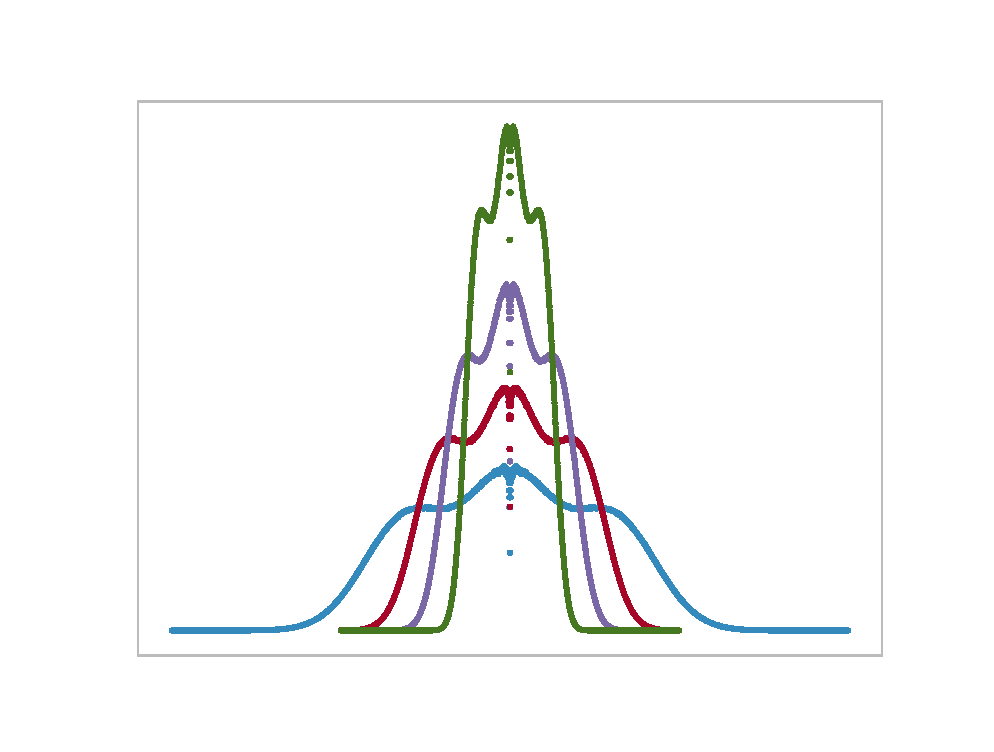
\includegraphics[scale=0.55]{../Images/art.eps}
	\caption{Radial one-body density profiles for two-dimensional quantum dots with $N=12$ electrons, popularly titled an artificial Magnesium atom. The four graphs correspond to four different oscillator frequencies, where the weakest oscillator gives the broadest density distribution.}
\end{figure}

We are finally ready to discuss the most exciting part of this thesis, namely the results. Since this work is associated with a degree in physics, the physical insights should be our focus and in this chapter we finally get the opportunity to discuss various physical interpretations of the results. Moreover, the various trial wave function ansätze used in variational Monte Carlo simulations (henceforth merely simulations) are discussed and compared. The Slater-Jastrow wave function is the \textit{de facto} standard ansatz used in variational Monte Carlo calculations of electronic structure problems. This ansatz, thoroughly discussed in chapter \ref{chp:methods}, is used as reference for our machine learning ansätze. Additionally, it is used for simulations of atomic systems, and will hereafter be abbreviated as the VMC ansatz. The most basic machine learning ansatz consists of a Slater determinant where the single-particle functions are determined by the marginal distributions of the visible nodes of a Gaussian-binary restricted Boltzmann machine. This is abbreviated as the RBM ansatz. When adding a simple Jastrow factor to this ansatz, we obtain the RBM+SJ ansatz. The RBM+PJ ansatz means that the Padé-Jastrow factor is added to the RBM ansatz. The respective Jastrow factors were discussed in section \ref{sec:jastrow}.

By using the implemented variational Monte Carlo framework described in chapter \ref{chp:WFE}, we can examine a large number of different systems. For quantum dot systems, the number of electrons, number of dimensions and oscillator frequency can all be varied. In total, we have looked at more than 150 different quantum dot systems using the four wave function ansätze mentioned above, which means that we have generated a large set of results. A selection of these results will be presented and discussed in this chapter, while a more extensive collection of results is presented in appendix \ref{chp:totalresults}. The results presented below have been selected since they describe physically interesting properties and allow for a comparison of the various ansätze. We will choose systems and configurations that can be compared with existing results. Our primary focus will be on ground state energy and electron density calculations, and we will stick to natural units as discussed in appendix \ref{app:units}. A brief recapitulation is that for quantum dots, the energy is given in units of Planck's reduced constant, $E'=E/\hbar$, and length is scaled as $x'=x/\sqrt{\hbar/m}$ with $m$ as the mass of an electron. This implies that the $d$-dimensional density, $\rho_d(\bs{r})$, is given in units of $(\hbar/m)^{-d/2}$. For atoms, we use Hartree atomic units, meaning that the length is given in units of the Bohr radius, $a_0$, the $d$-dimensional density is given in units of $a_0^{-d}$ and the energy is scaled as $E'=E/(\hbar^2/m_ea_0)$.

Before we move on to the physical results, we will take a quick look at some more technical results. More precisely, we will discuss the computational cost of the various ansätze and the energy convergence using various optimization tools. For validation purposes, we will present a few selected results on the case without repulsive interaction and compare it to analytical results. After that, we study the case with repulsive interaction on a much larger scale, where we first look at quantum dots and then on atoms. 

\begin{figure}
	\centering 
	% This file was created by matplotlib2tikz v0.7.4.
\begin{tikzpicture}[scale=0.9]

\begin{axis}[name=2D, xlabel=$N$, ylabel={CPU-time [s]}, grid=major, 
legend cell align={left},
legend style={at={(1.68,1.10)}, anchor=south east, draw=white!80.0!black},
legend columns = 6, 
clip=false,
xtick=data] 
\addplot[color=color0,mark=oplus*, dashed] coordinates { 
	(2,6.05)
	(6,11.25)
	(12,20.53) 
	(20,38.99) 
	(30,73.73) 
	(42,130.49) 
	(56,213.47)
	(72,360.22)
	(90,856.84) }; 
\addlegendentry{RBM};

\addplot[color=color1,mark=oplus*, dash dot] coordinates { 
	(2,7.12) 
	(6,14.07) 
	(12,28.42) 
	(20,63.27) 
	(30,122.93) 
	(42,199.60)
	(56,349.22)}; 
\addlegendentry{RBM+SJ};

\addplot[color=color2,mark=oplus*, dotted] coordinates { 
	(2,7.26)
	(6,13.50)
	(12,27.68)
	(20,57.09) 
	(30,119.17) 
	(42,212.53) 
	(56,382.13) }; 
\addlegendentry{RBM+PJ};

\addplot[color=color3,mark=oplus*] coordinates { 
	(2,5.11)
	(6,10.51)
	(12,20.85) 
	(20,41.20) 
	(30,76.26) 
	(42,137.39) 
	(56,230.63)
	(72,355.81)
	(90,544.03) }; 
\addlegendentry{VMC};

\node[] at (axis cs: 44,978) {2D};
\end{axis}

\begin{axis}[name=2D, 
xshift=7.9cm, 
xlabel=$N$, 
grid=major, 
clip=false,
xtick=data] 
\addplot[color=color0,mark=oplus*, dashed] coordinates { 
	(2,7.69)
	(8,20.92)
	(20,59.67) 
	(40,171.84) 
	(70,586.39) }; 
%\addlegendentry{RBM};

\addplot[color=color1,mark=oplus*, dash dot] coordinates { 
	(2,8.95)
	(8,26.86)
	(20,94.64) 
	(40,270.92) }; 
%\addlegendentry{RBM+SJ};

\addplot[color=color2,mark=oplus*, dotted] coordinates { 
	(2,8.87)
	(8,26.36)
	(20,91.40) 
	(40,293.25) }; 
%\addlegendentry{RBM+PJ};

\addplot[color=color3,mark=oplus*] coordinates { 
	(2,6.70)
	(8,20.99)
	(20,62.54) 
	(40,185.65) 
	(70,486.02) };
%\addlegendentry{VMC};

\node[] at (axis cs: 35,670) {3D};
\end{axis}
\end{tikzpicture}
	\caption{CPU-time per iteration as a function of the number of electrons, $N$, for two-dimensional (2D) and three-dimensional (3D) quantum dots. The number of Monte Carlo cycles per iteration is $M=2^{20}=1,048,576$. For more details see the text and appendix \ref{chp:totalresults}.}
	\label{fig:cpu_time}
\end{figure} 

\section{Computational cost}
Quantum many-body simulations are frequently ranked among the most computationally intensive fields. A reason for this is the large amount of information stored in the wave function. Albeit the VMC ansatz is known to have a high performance-to-cost ratio, it is still not cheap. In this section, we will find the average cost of the VMC ansatz and compare it to the cost of the machine learning ansätze described above. In figure \eqref{fig:cpu_time}, the CPU-time is plotted as a function of the number of electrons, $N$, for two-dimensional (left) and three-dimensional (right) quantum dots. To obtain accurate CPU-times, all the simulations were run on the Abel computer cluster with $M=2^{20}=1,048,576$ Monte Carlo cycles per iteration. The time presented is the average time over at least four independent runs with thousands of iterations each. For more details, see appendix \ref{chp:totalresults}, section \ref{sec:cputime}.

\begin{table}
	\caption{The scaling of the computational cost for two-dimensional (2D) and three-dimensional (3D) quantum dots as a function of the number of electrons, $N$. The numbers presented in the table are the optimal $b$-value found from fitting the power function $f(N)=0.5N^b$ to the cost graph. For abbreviations see the text.}
	\begin{tabularx}{\textwidth}{CCCCC} \hline\hline
		\label{tab:cputimefit}
		\makecell{\\ \phantom{=}} & RBM & RBM+SJ & RBM+PJ & VMC \\ \hline \\
		2D & 1.498 & 1.639 & 1.621 & 1.515 \\ 
		3D & 1.584 & 1.710 & 1.729 & 1.605 \\ \hline\hline
	\end{tabularx}
\end{table} 

Our immediate observation is that the ansätze are pairwise quite similar, with the RBM and VMC as the cheapest ones, and the RBM+SJ and RBM+PJ as the most expensive. This is not surprising, as RBM requires a neural network, VMC requires a Jastrow factor while RBM+SJ and RBM+PJ require both a neural network and a Jastrow factor. For two-dimensional dots, RBM is the cheapest among all the ansätze, but for larger systems ($N=42,56$), VMC is cheaper due to an explosion in CPU-time for the RBM ansatz. This explosion can be explained by our choice of the number of hidden nodes, $H$, which consequently is set to the number of electrons, i.e. $H=N$, which was found to give the lowest energy for small quantum dots\supercite{flugsrud_vilde_moe_solving_nodate}. Since the RBM ansatz has $N\cdot d\cdot (1+H)+H$ variational parameters with $d$ as the number of dimensions, the number of variational parameters for a two-dimensional dot with $N=90$ electrons is 16,470. On the other hand, the VMC ansatz is equipped with two variational parameters for all system sizes, which obviously makes the parameter update less costly. We also observe that the RBM+PJ ansatz is cheaper than the RBM+SJ ansatz for systems up to $N=42$, but after that, the RBM+SJ ansatz is slightly cheaper. This might be surprising, as the simple Jastrow factor contains $N^2$ variational parameters, but a possible explanation is that BLAS is optimized for large matrix-vector operations and is thus fully utilized first when the matrices get large. We observe the same behavior for the three-dimensional dots as for the two-dimensional dots, and the discussion above is representative for them as well.

The standard way of estimating the scaling of variational Monte Carlo simulations is to fit the power functions, $f(x)=ax^b$, to the cost graphs. As all the simulations were performed with the same hyper-parameters and with equal external factors. We fix the first parameter by setting $a=0.5$, as this was found to be a reasonable average value based on two-parameter fitting. In that manner, we can focus on optimizing $b$ only, which is the parameter that specifies the scaling, i.e.; we say that the method scales as $N^b$. In table \eqref{tab:cputimefit}, the optimal $b$ from linear regression is presented for our four ansätze for two- and three-dimensional quantum dots. We want to emphasize that we only did the regression for CPU-times up to $N=56$ in two-dimensional dots and $N=40$ in three-dimensional dots, partly because we only have data for all methods in this interval and partly because the CPU-time for the RBM explodes for large dots. We believe that this was the best way to do it in order to make the various methods comparable. 

The numbers in the table match our impression from figure \eqref{fig:cpu_time}, where RBM and VMC were found to be more expensive than RBM+SJ and RBM+PJ. For all the ansätze, the scaling was found to be between linear and quadratic as a function of the number of electrons, which is surprising as the update of the Slater matrix scales as $\sim N^2$. 

\section{Energy convergence}
We always want our simulations to converge fast and to be stable, which the optimization tool is responsible for. In figure \eqref{fig:convergenceoptimization}, we compare standard gradient descent (GD) to stochastic gradient descent (SGD) and ADAM for two- and three-dimensional quantum dots with $N=2$ interacting electrons. The optimization algorithms were detailed in section \ref{sec:optimizationalgorithms}. The gradient descent methods are plain, meaning it is without momentum and adaptive learning rate, while the ADAM optimizer has momentum and adaptivity by nature. The frequency $\omega=1.0$ is used for the two-dimensional case since the analytical energy, $E=3.0$, is available \supercite{taut_two_1993}. Similarly, we use the frequency $\omega=0.5$ for the three-dimensional case since the exact energy is $E=2.0$ \supercite{taut_two_1994}. 

\begin{figure}
	\centering 
	\subfloat{{\begin{tikzpicture} [scale=0.9, spy using outlines=
	{rectangle, magnification=8,size=2cm, height=1cm, connect spies}]
	\begin{axis} [name=2D, 
	xlabel=Iteration, 
	ylabel={Energy [Ha]}, 
	grid=major, 
	clip=false,
	every axis plot/.append style={thick},
	legend cell align={left},
	legend style={at={(1.45,1.1)}, anchor=south east, draw=white!80.0!black},
	legend columns = 6
	]
	
	\addplot[color2] table [x expr=\coordindex+1, 
	y index=0, 
	mark=none] {/home/evenmn/VMC/data/int1/quantumdot/energy/VMC/2D/2P/1.000000w/GD_MC16777216.dat};
	\addlegendentry{GD};
	
	\addplot[color1] table [x expr=\coordindex+1, 
	y index=0, 
	mark=none] {/home/evenmn/VMC/data/int1/quantumdot/energy/VMC/2D/2P/1.000000w/SGD_MC16777216.dat}; 
	\addlegendentry{SGD};
	
	\addplot[color0] table [x expr=\coordindex+1, 
	y index=0, 
	mark=none, 
	color=blue] {/home/evenmn/VMC/data/int1/quantumdot/energy/VMC/2D/2P/1.000000w/ADAM_MC16777216.dat}; 
	\addlegendentry{ADAM};
	
	\addplot [dashed,mark=none,black] coordinates {(0,3) (100,3)};
	\addlegendentry{Exact};
	
	\node[] at (axis cs: 50,3.178) {2D, $\omega=1.0$};
	\coordinate (spypoint1) at (axis cs:75,2.995001);
	\coordinate (magnifyglass1) at (axis cs:50,3.1);
	\end{axis}
	\spy [size=2.0cm] on (spypoint1)
	in node[fill=white] at (magnifyglass1);
	
	\begin{axis} [name=3D, 
	xshift=7.9cm, 
	xlabel=Iteration, 
	grid=major, 
	clip=false,
	every axis plot/.append style={thick}]	
	\addplot[color2] table[x expr=\coordindex+1, y index=0, mark=none] {/home/evenmn/VMC/data/int1/quantumdot/energy/VMC/3D/2P/0.500000w/GD_MC16777216.dat};  
	%\addlegendentry{GD};
	
	\addplot[color1] table[x expr=\coordindex+1, y index=0, mark=none] {/home/evenmn/VMC/data/int1/quantumdot/energy/VMC/3D/2P/0.500000w/SGD_MC16777216.dat};  
	%\addlegendentry{SGD};
	
	\addplot[color0] table[x expr=\coordindex+1, y index=0, mark=none] {/home/evenmn/VMC/data/int1/quantumdot/energy/VMC/3D/2P/0.500000w/ADAM_MC16777216.dat}; 
	%\addlegendentry{ADAM};
	
	\addplot+ [dashed,mark=none,color=black] coordinates {(0,2) (100,2)};
	%\addlegendentry{Exact};
	
	\node[] at (axis cs: 50,2.1355) {3D, $\omega=0.5$};
	\coordinate (spypoint2) at (axis cs:75,1.997);
	\coordinate (magnifyglass2) at (axis cs:50,2.077);
	\end{axis} 
	\spy [size=2.0cm] on (spypoint2)
	in node[fill=white] at (magnifyglass2);
\end{tikzpicture}}}
	\caption{Convergence of the obtained ground state energy, $E$, for quantum dots with $N=2$ in two dimensions (2D) with frequency $\omega=1.0$ (left) and in three dimensions (3D) with frequency $\omega=0.5$ (right). The VMC ansatz was used, described in the text, and the optimization tools gradient descent (GD), stochastic gradient descent with 10 batches (SGD) and the ADAM optimizer are all compared. Semi-analytical energies (Exact) are taken from \citet{taut_two_1993} (2D) and \citet{taut_two_1994} (3D). The learning rate was set to $\eta=0.5$ and the number of Metropolis steps was $M=2^{24}=16,777,216$. All energies are given in units of $\hbar$ (natural units).}
	\label{fig:convergenceoptimization}
\end{figure} 

The first thing we observe is that all three optimization tools manage to converge to a value close to the exact energy (see spy window). The stochastic and non-stochastic gradient descent methods behave similarly, but we observe that the SGD goes below the exact energy before it stabilizes. The ADAM optimizer, fluctuates much more, which can be explained by the momentum, as discussed in section \ref{sec:momentum}. It is also important to remember that we use the VMC ansatz, which is equipped with two variational parameters only, and thus is easier to control. The ADAM optimizer is known to be good at minimizing functions with many variational parameters, so we will stick to it even though gradient descent seems like a clever choice seen from the figure. Another point is that the quantum dots have neat potentials without local minima. When we move on to more complex systems, ADAM generally works better according to the literature \supercite{kingma_adam:_2014}.

\begin{figure}
	\centering 
	\subfloat{{% This file was created by tikzplotlib v0.8.1.
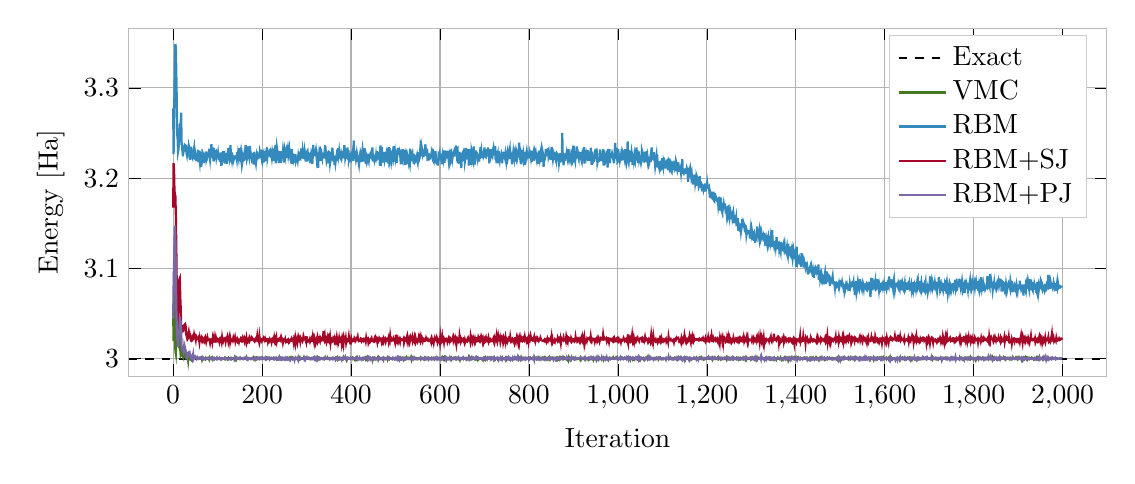
\begin{tikzpicture}

\definecolor{color0}{rgb}{0.203921568627451,0.541176470588235,0.741176470588235}
\definecolor{color1}{rgb}{0.650980392156863,0.0235294117647059,0.156862745098039}
\definecolor{color2}{rgb}{0.47843137254902,0.407843137254902,0.650980392156863}
\definecolor{color3}{rgb}{0.274509803921569,0.470588235294118,0.129411764705882}

\begin{axis}[
axis line style={white!73.72549019607844!black},
legend cell align={left},
legend style={draw=white!80.0!black},
tick pos=both,
x grid style={white!69.80392156862744!black},
xlabel={Iteration},
xmajorgrids,
xmin=-99.9499999999999, xmax=2098.95,
width=14cm,
height=6cm,
xtick style={color=black},
y grid style={white!69.80392156862744!black},
ylabel={Energy [Ha]},
ymajorgrids,
ymin=2.9807755, ymax=3.3660945,
ytick style={color=black}
]
\addplot [thick, black, dashed]
table {%
-99.9499999999999 3
2098.95 3
};
\addlegendentry{Exact}
\addplot [thick, color3]
table {%
-1.98991768347129e-15 3.04959
0.999999999999998 3.01958
2 3.09682
3 3.08172
4 3.04253
5 3.0082
6 3.00532
7 3.02106
8 3.03036
9 3.03826
10 3.02706
11 3.01589
12 3.01468
13 3.02001
14 3.03229
15 3.02307
16 3.00997
17 3.00401
18 3.00495
19 3.0102
20 3.00783
21 3.0048
22 3.002
23 3.00101
24 3.00527
24.9999999999995 3.00544
25.9999999999995 3.00456
26.9999999999995 3.00586
27.9999999999994 3.00346
28.9999999999994 3.00136
29.9999999999994 3.00207
30.9999999999994 3.00605
31.9999999999994 3.00601
32.9999999999993 3.00376
33.9999999999993 2.9984
34.9999999999993 3.00272
35.9999999999993 3.00149
36.9999999999993 3.00122
37.9999999999992 3.00043
38.9999999999992 3.0019
39.9999999999992 3.00017
40.9999999999992 2.99925
41.9999999999992 3.00079
42.9999999999991 3.0015
43.9999999999991 3.00268
44.9999999999991 3.00125
45.9999999999991 3.00077
46.9999999999991 3.00108
47.999999999999 3.00081
48.999999999999 3.00069
49.999999999999 3.0012
50.999999999999 3.00091
51.999999999999 3.00107
52.9999999999989 3.00045
53.9999999999989 3.00096
54.9999999999989 3.00126
55.9999999999989 3.00055
56.9999999999989 3.00051
57.9999999999988 3.00077
58.9999999999988 3.00047
59.9999999999988 2.99992
60.9999999999988 3.00023
61.9999999999988 3.00115
62.9999999999987 3.00086
63.9999999999987 3.0013
64.9999999999987 2.99916
65.9999999999987 3.00076
66.9999999999987 3.00077
67.9999999999986 2.99959
68.9999999999986 2.99972
69.9999999999986 3.00035
70.9999999999986 3.0005
71.9999999999986 2.99972
72.9999999999985 3.00071
73.9999999999985 2.99981
74.9999999999985 3.00037
75.9999999999985 3.00064
76.9999999999985 3.001
77.9999999999984 3.0008
78.9999999999984 3.00024
79.9999999999984 3.00066
80.9999999999984 2.99937
81.9999999999984 3.00116
82.9999999999983 3.00023
83.9999999999983 3.00099
84.9999999999983 3.00101
85.9999999999983 3.00018
86.9999999999983 2.99954
87.9999999999982 2.99974
88.9999999999982 3.00119
89.9999999999982 3.00059
90.9999999999982 3.00008
91.9999999999982 2.99958
92.9999999999982 3.00056
93.9999999999981 2.99999
94.9999999999981 3.00059
95.9999999999981 3.00049
96.9999999999981 3.00068
97.999999999998 3.00095
98.999999999998 3.0011
99.999999999998 3.00066
100.999999999998 2.99999
101.999999999998 3.0002
102.999999999998 2.99977
103.999999999998 2.99986
104.999999999998 2.99996
105.999999999998 2.99957
106.999999999998 3.00038
107.999999999998 3.00063
108.999999999998 3.00069
109.999999999998 3.00033
110.999999999998 3.00007
111.999999999998 2.99969
112.999999999998 2.99967
113.999999999998 2.99986
114.999999999998 3.00042
115.999999999998 3.00102
116.999999999998 2.99985
117.999999999998 3.00066
118.999999999998 3.00076
119.999999999998 3.00062
120.999999999998 3.00065
121.999999999998 2.99976
122.999999999998 3.00064
123.999999999998 3.00107
124.999999999998 2.99983
125.999999999997 3.00025
126.999999999997 3.00057
127.999999999997 3.00052
128.999999999997 3.00074
129.999999999997 3.001
130.999999999997 3.00044
131.999999999997 3.0009
132.999999999997 3.00051
133.999999999997 3.00059
134.999999999997 3.00068
135.999999999997 3.00059
136.999999999997 3.00024
137.999999999997 3.00033
138.999999999997 3.00023
139.999999999997 2.99941
140.999999999997 3.00082
141.999999999997 2.99928
142.999999999997 3.0004
143.999999999997 3.00078
144.999999999997 3.00102
145.999999999997 3.00004
146.999999999997 3.00006
147.999999999997 3.00042
148.999999999997 3.00075
149.999999999997 3.00121
150.999999999997 3.00014
151.999999999997 3.00038
152.999999999997 3.00035
153.999999999997 3.00059
154.999999999997 3.00063
155.999999999997 2.99972
156.999999999997 2.99978
157.999999999997 3.00029
158.999999999997 3.0003
159.999999999997 3.00087
160.999999999997 3.00058
161.999999999997 3.00013
162.999999999997 3.00025
163.999999999997 3.00131
164.999999999997 3.0008
165.999999999997 2.99977
166.999999999997 3.00037
167.999999999997 3.00065
168.999999999997 3.00004
169.999999999997 3.00055
170.999999999997 3.00078
171.999999999997 3.0004
172.999999999997 3.00006
173.999999999997 3.00036
174.999999999996 3.00023
175.999999999996 3.0002
176.999999999996 2.99961
177.999999999996 2.99979
178.999999999996 3.00008
179.999999999996 3.00116
180.999999999996 3.00009
181.999999999996 3.00093
182.999999999996 3.00048
183.999999999996 2.99932
184.999999999996 3.00074
185.999999999996 3.00032
186.999999999996 2.99986
187.999999999996 3.00151
188.999999999996 3.00124
189.999999999996 3.00039
190.999999999996 2.99968
191.999999999996 2.99979
192.999999999996 2.99993
193.999999999996 3.00056
194.999999999996 2.99974
195.999999999996 3.00003
196.999999999996 2.99999
197.999999999996 3.00008
198.999999999996 2.99965
199.999999999996 2.99952
200.999999999996 2.99966
201.999999999996 3.00087
202.999999999996 3.0002
203.999999999996 3.00023
204.999999999996 3.00071
205.999999999996 3.00084
206.999999999996 3.00019
207.999999999996 3.00083
208.999999999996 3.00021
209.999999999996 3.00161
210.999999999996 3.0014
211.999999999996 3.00093
212.999999999996 3.00067
213.999999999996 3.00072
214.999999999996 3.00047
215.999999999996 3.00116
216.999999999996 3.00057
217.999999999996 3.00099
218.999999999996 3.00083
219.999999999996 3.00017
220.999999999996 3.00061
221.999999999996 3.00011
222.999999999996 3.00008
223.999999999996 3.00072
224.999999999995 3.00051
225.999999999995 3.001
226.999999999995 2.99968
227.999999999995 3.0001
228.999999999995 2.99996
229.999999999995 3.00096
230.999999999995 3.00069
231.999999999995 3.00017
232.999999999995 3.00013
233.999999999995 3.00029
234.999999999995 2.99987
235.999999999995 2.99951
236.999999999995 2.99928
237.999999999995 2.99985
238.999999999995 3.00149
239.999999999995 3.00013
240.999999999995 3.00063
241.999999999995 3.00052
242.999999999995 2.99984
243.999999999995 3.00073
244.999999999995 3.0003
245.999999999995 3.00071
246.999999999995 3.0004
247.999999999995 3.00014
248.999999999995 3.00035
249.999999999995 3.00049
250.999999999995 3.00084
251.999999999995 3.00062
252.999999999995 2.99993
253.999999999995 2.99999
254.999999999995 3.00009
255.999999999995 2.99968
256.999999999995 3.00057
257.999999999995 2.99973
258.999999999995 3.00023
259.999999999995 3.00008
260.999999999995 3.00069
261.999999999995 2.99974
262.999999999995 2.99909
263.999999999995 3.00078
264.999999999995 3.00003
265.999999999995 3.0003
266.999999999995 3.00118
267.999999999995 3.00026
268.999999999995 3.00108
269.999999999995 3.0005
270.999999999995 3.00086
271.999999999995 3.00032
272.999999999995 2.99996
273.999999999995 3.00031
274.999999999994 3.00049
275.999999999994 3.0004
276.999999999994 2.99972
277.999999999994 2.99981
278.999999999994 3.00009
279.999999999994 3.0008
280.999999999994 3.00134
281.999999999994 2.99921
282.999999999994 3.00043
283.999999999994 2.99989
284.999999999994 3.00122
285.999999999994 2.99993
286.999999999994 3.00067
287.999999999994 3.00084
288.999999999994 3.00074
289.999999999994 3.0003
290.999999999994 3.00023
291.999999999994 3.00006
292.999999999994 2.99994
293.999999999994 3.00127
294.999999999994 2.99978
295.999999999994 2.99995
296.999999999994 3.00058
297.999999999994 3.00063
298.999999999994 3.00099
299.999999999994 3.00037
300.999999999994 2.99998
301.999999999994 3
302.999999999994 3.00027
303.999999999994 3.00065
304.999999999994 3.00115
305.999999999994 3.00079
306.999999999994 2.99971
307.999999999994 2.99951
308.999999999994 3.00035
309.999999999994 3.00046
310.999999999994 3.00071
311.999999999994 3.00005
312.999999999994 3.00053
313.999999999994 3.00034
314.999999999994 3.00092
315.999999999994 3.00006
316.999999999994 2.99984
317.999999999994 2.99995
318.999999999994 3.00052
319.999999999994 2.99981
320.999999999994 3.00075
321.999999999994 3.00063
322.999999999994 3.00086
323.999999999993 3.00146
324.999999999994 2.99934
325.999999999994 3.00023
326.999999999993 3.00002
327.999999999993 2.99969
328.999999999993 3.00117
329.999999999993 3.00083
330.999999999993 3.00055
331.999999999993 3.00028
332.999999999993 3.00071
333.999999999993 3.00057
334.999999999993 3.00039
335.999999999993 3.00028
336.999999999993 3.00048
337.999999999993 3.00048
338.999999999993 3.0005
339.999999999993 2.99931
340.999999999993 2.9997
341.999999999993 3.00011
342.999999999993 3.00046
343.999999999993 3.00032
344.999999999993 3.00035
345.999999999993 3.00053
346.999999999993 3.00146
347.999999999993 3.00063
348.999999999993 2.99984
349.999999999993 2.99974
350.999999999993 2.99991
351.999999999993 3.0007
352.999999999993 3.00045
353.999999999993 3.0001
354.999999999993 2.99971
355.999999999993 2.99988
356.999999999993 2.99984
357.999999999993 2.99996
358.999999999993 3.00102
359.999999999993 3.00093
360.999999999993 3.00079
361.999999999993 2.99995
362.999999999993 2.99982
363.999999999993 3.0008
364.999999999993 3.00117
365.999999999993 2.9997
366.999999999993 3.00013
367.999999999993 3.00017
368.999999999993 2.99938
369.999999999993 3.00128
370.999999999993 3.00061
371.999999999993 3.00068
372.999999999993 2.99975
373.999999999993 3.00025
374.999999999992 3.00094
375.999999999992 3.00014
376.999999999992 3.00048
377.999999999992 2.99996
378.999999999992 3.00032
379.999999999992 3.00029
380.999999999992 3.00065
381.999999999992 3.00008
382.999999999992 3.00158
383.999999999992 3.0006
384.999999999992 3.0001
385.999999999992 2.99983
386.999999999992 3.00084
387.999999999992 3.00007
388.999999999992 3.00045
389.999999999992 2.99889
390.999999999992 3.00046
391.999999999992 3.00032
392.999999999992 3.00082
393.999999999992 3.00015
394.999999999992 3.00046
395.999999999992 3.00014
396.999999999992 3.00029
397.999999999992 3.00036
398.999999999992 3.00107
399.999999999992 3.00057
400.999999999992 3.00062
401.999999999992 3.00031
402.999999999992 3.00086
403.999999999992 2.9996
404.999999999992 2.9998
405.999999999992 3.00076
406.999999999992 3.00047
407.999999999992 2.99939
408.999999999992 3.00018
409.999999999992 3.00075
410.999999999992 2.99936
411.999999999992 3.00044
412.999999999992 2.99971
413.999999999992 3.00112
414.999999999992 2.99984
415.999999999992 2.99946
416.999999999992 3.00029
417.999999999992 3.00045
418.999999999992 2.99998
419.999999999992 3
420.999999999992 3.00029
421.999999999992 3.00055
422.999999999992 3.00008
423.999999999991 3.00002
424.999999999991 2.99984
425.999999999991 3.00051
426.999999999991 2.99987
427.999999999991 2.99984
428.999999999991 3.00067
429.999999999991 2.99974
430.999999999991 2.99977
431.999999999991 3.00064
432.999999999991 2.99956
433.999999999991 3.00072
434.999999999991 2.99988
435.999999999991 3.00107
436.999999999991 2.9997
437.999999999991 3.00013
438.999999999991 3.00016
439.999999999991 3.00027
440.999999999991 3.00019
441.999999999991 3.00079
442.999999999991 3.00011
443.999999999991 2.99942
444.999999999991 3.00052
445.999999999991 3.00037
446.999999999991 3.00064
447.999999999991 3.00009
448.999999999991 2.99953
449.999999999991 3.00039
450.999999999991 2.99952
451.999999999991 3.00041
452.999999999991 3.00085
453.999999999991 3.0004
454.999999999991 2.99956
455.999999999991 3.00005
456.999999999991 2.99998
457.999999999991 3.00076
458.999999999991 3.00093
459.999999999991 3.00163
460.999999999991 2.99961
461.999999999991 3.00127
462.999999999991 3.00037
463.999999999991 3.00101
464.999999999991 3
465.999999999991 3.00035
466.999999999991 3.00031
467.999999999991 3.0005
468.999999999991 3.00046
469.999999999991 2.99984
470.999999999991 3.00073
471.999999999991 3.00054
472.999999999991 3.00012
473.999999999991 3.00086
474.99999999999 3.00006
475.99999999999 3.00008
476.99999999999 2.99979
477.99999999999 3.00058
478.99999999999 3.00039
479.99999999999 3
480.99999999999 3.00073
481.99999999999 2.99938
482.99999999999 3.00118
483.99999999999 3.00047
484.99999999999 3.00008
485.99999999999 3.00041
486.99999999999 2.99986
487.99999999999 3.0007
488.99999999999 3.00069
489.99999999999 3.00027
490.99999999999 2.99984
491.99999999999 2.99976
492.99999999999 3.00008
493.99999999999 3.00012
494.99999999999 3.00074
495.99999999999 3.0006
496.99999999999 3.00067
497.99999999999 2.99977
498.99999999999 3.00051
499.99999999999 2.99986
500.99999999999 2.99957
501.99999999999 3.00048
502.99999999999 3.00069
503.99999999999 3.00008
504.99999999999 3.00098
505.99999999999 3.00009
506.99999999999 2.99986
507.99999999999 3.001
508.99999999999 3.00026
509.99999999999 2.99974
510.99999999999 3.00079
511.99999999999 3.00014
512.99999999999 3.0002
513.99999999999 3.00062
514.99999999999 2.99998
515.99999999999 3.00008
516.99999999999 2.99993
517.99999999999 2.99986
518.99999999999 3.00072
519.99999999999 2.99974
520.99999999999 3.00084
521.99999999999 3.00087
522.99999999999 3.00011
523.99999999999 2.99989
524.999999999989 3.00115
525.999999999989 2.99985
526.99999999999 3
527.99999999999 3.00041
528.999999999989 3.0012
529.999999999989 3.00122
530.999999999989 3.00087
531.999999999989 3.0005
532.999999999989 2.99982
533.999999999989 2.99986
534.999999999989 3.00136
535.999999999989 2.99942
536.999999999989 3.00139
537.999999999989 3.00069
538.999999999989 3.00015
539.999999999989 3.00037
540.999999999989 3.00016
541.999999999989 3.00122
542.999999999989 3.00034
543.999999999989 2.9996
544.999999999989 2.9997
545.999999999989 2.99957
546.999999999989 3.00051
547.999999999989 3.00006
548.999999999989 2.99989
549.999999999989 3.00045
550.999999999989 3.00064
551.999999999989 2.9999
552.999999999989 2.99998
553.999999999989 2.99998
554.999999999989 2.99976
555.999999999989 3.00075
556.999999999989 2.99952
557.999999999989 3.00022
558.999999999989 2.99982
559.999999999989 3.00007
560.999999999989 3.00034
561.999999999989 2.99978
562.999999999989 3.00056
563.999999999989 3.00016
564.999999999989 2.99957
565.999999999989 3.00108
566.999999999989 3.00056
567.999999999989 3.00023
568.999999999989 3.00051
569.999999999989 3.00014
570.999999999989 3.00001
571.999999999989 3.00065
572.999999999989 3.00054
573.999999999989 3.00118
574.999999999988 3.00044
575.999999999988 3.00007
576.999999999988 3.00066
577.999999999989 3.00052
578.999999999988 3.0003
579.999999999989 3
580.999999999988 3.0007
581.999999999988 2.99961
582.999999999988 3.00031
583.999999999988 3.00059
584.999999999988 3.00109
585.999999999988 3.00057
586.999999999988 3.00047
587.999999999988 2.99994
588.999999999988 3.0007
589.999999999988 3.00089
590.999999999988 3.00084
591.999999999988 3.00052
592.999999999988 3.00113
593.999999999988 3.00044
594.999999999988 3.00018
595.999999999988 2.99952
596.999999999988 2.99992
597.999999999988 3.00087
598.999999999988 3.00047
599.999999999988 2.99971
600.999999999988 3.00028
601.999999999988 3.00021
602.999999999988 3.00071
603.999999999988 2.99994
604.999999999988 2.9997
605.999999999988 3.00102
606.999999999988 3.00004
607.999999999988 3.00096
608.999999999988 3.00157
609.999999999988 2.99919
610.999999999988 2.99994
611.999999999988 3.00061
612.999999999988 3.00088
613.999999999988 3.00039
614.999999999988 3.00034
615.999999999988 3.00075
616.999999999988 3.00095
617.999999999988 3.00038
618.999999999988 3.0005
619.999999999987 3.00032
620.999999999987 3.0012
621.999999999987 3.00135
622.999999999987 3.0008
623.999999999987 3.00006
624.999999999987 2.99927
625.999999999987 3.00077
626.999999999988 2.99992
627.999999999987 2.99978
628.999999999987 2.99999
629.999999999987 3.0007
630.999999999987 3.00011
631.999999999987 3.00074
632.999999999987 3.00038
633.999999999987 2.99997
634.999999999987 3.00103
635.999999999987 3.00041
636.999999999987 3.00064
637.999999999987 3.00103
638.999999999987 2.99977
639.999999999987 2.99959
640.999999999987 3.00022
641.999999999987 3.00011
642.999999999987 3.00063
643.999999999987 3.00066
644.999999999987 2.99905
645.999999999987 3.00067
646.999999999987 3.00069
647.999999999987 3.00048
648.999999999987 3.00045
649.999999999987 3.00053
650.999999999987 3.00029
651.999999999987 3.00012
652.999999999987 3
653.999999999987 3.00027
654.999999999987 3.00031
655.999999999987 3.0007
656.999999999987 3.00011
657.999999999987 3.00071
658.999999999987 3.0009
659.999999999987 3.00054
660.999999999987 3.00045
661.999999999987 2.99981
662.999999999987 3.00054
663.999999999987 2.99998
664.999999999987 3.00175
665.999999999987 3.00041
666.999999999987 3.00039
667.999999999987 3.00096
668.999999999987 3.00048
669.999999999987 3.00043
670.999999999987 3.00127
671.999999999987 2.99965
672.999999999987 2.9995
673.999999999986 3.00004
674.999999999986 3.00086
675.999999999986 3.00038
676.999999999986 3.00065
677.999999999986 3.00037
678.999999999986 3.00009
679.999999999986 2.99952
680.999999999986 3.00046
681.999999999986 3.00035
682.999999999986 3.00093
683.999999999986 2.99962
684.999999999986 3.00101
685.999999999986 3.00047
686.999999999986 2.9995
687.999999999986 3.00024
688.999999999986 3.0004
689.999999999986 3.00071
690.999999999986 3.00017
691.999999999986 3.00029
692.999999999986 3.00061
693.999999999986 3.00012
694.999999999986 3.00017
695.999999999986 3.00039
696.999999999986 2.99918
697.999999999986 3.00067
698.999999999986 2.99997
699.999999999986 2.99963
700.999999999986 3.00041
701.999999999986 2.99954
702.999999999986 3.00112
703.999999999986 3.00036
704.999999999986 3.00004
705.999999999986 2.99953
706.999999999986 2.99993
707.999999999986 3.00124
708.999999999986 3.00071
709.999999999986 3.00109
710.999999999986 3.00139
711.999999999986 3.00027
712.999999999986 3.00035
713.999999999986 3.0006
714.999999999986 2.99989
715.999999999986 3.00092
716.999999999986 3.00034
717.999999999986 3.0002
718.999999999986 3.00004
719.999999999986 3.0001
720.999999999986 2.99987
721.999999999986 3.00118
722.999999999986 3
723.999999999986 2.99944
724.999999999985 3.00086
725.999999999986 3.00095
726.999999999985 3.00086
727.999999999986 3.00016
728.999999999985 3.00045
729.999999999985 2.99998
730.999999999985 3.00017
731.999999999985 2.99915
732.999999999985 3.00031
733.999999999985 3.00059
734.999999999985 3.00064
735.999999999985 3.00049
736.999999999985 3.00006
737.999999999985 3.00043
738.999999999985 2.99981
739.999999999985 3.00091
740.999999999985 2.99955
741.999999999985 2.99979
742.999999999985 2.9998
743.999999999985 3.00068
744.999999999985 3.0006
745.999999999985 3.00055
746.999999999985 2.99969
747.999999999985 3.0008
748.999999999985 2.99954
749.999999999985 3.00098
750.999999999985 3.00041
751.999999999985 3.00082
752.999999999985 2.99992
753.999999999985 3.00048
754.999999999985 3.00062
755.999999999985 3.00075
756.999999999985 3.00045
757.999999999985 2.99955
758.999999999985 3.00029
759.999999999985 3.00011
760.999999999985 3.00065
761.999999999985 3.00065
762.999999999985 3.00014
763.999999999985 2.99981
764.999999999985 3.00077
765.999999999985 3.00045
766.999999999985 3.00101
767.999999999985 3.00023
768.999999999985 3.00022
769.999999999985 3.00066
770.999999999985 3.00066
771.999999999985 3.00005
772.999999999985 2.99957
773.999999999984 2.99991
774.999999999985 3.0011
775.999999999985 2.99986
776.999999999984 3.0013
777.999999999984 3.00007
778.999999999984 2.99982
779.999999999984 3.00018
780.999999999984 3.00017
781.999999999984 3.00133
782.999999999984 2.99931
783.999999999984 2.99997
784.999999999984 2.99981
785.999999999984 2.99996
786.999999999984 3.00109
787.999999999984 3.00079
788.999999999984 3.00014
789.999999999984 3.0006
790.999999999984 3.00106
791.999999999984 3.0008
792.999999999984 3.00044
793.999999999984 3.00058
794.999999999984 3.00063
795.999999999984 3.00011
796.999999999984 3.0002
797.999999999984 3.0007
798.999999999984 3.00137
799.999999999984 3.00085
800.999999999984 2.99954
801.999999999984 3.00025
802.999999999984 3.00085
803.999999999984 3.00029
804.999999999984 3.0001
805.999999999984 3.00025
806.999999999984 3.00058
807.999999999984 3.00039
808.999999999984 3.00103
809.999999999984 3.00044
810.999999999984 3.00044
811.999999999984 3.00008
812.999999999984 3.00042
813.999999999984 3.00037
814.999999999984 3.00113
815.999999999984 3.00118
816.999999999984 3.00013
817.999999999984 3.00105
818.999999999984 2.99985
819.999999999984 3.00001
820.999999999984 3.00008
821.999999999984 3.00104
822.999999999983 2.9995
823.999999999984 2.99991
824.999999999984 3.0007
825.999999999983 3.00035
826.999999999984 3.00029
827.999999999983 2.99992
828.999999999984 3.00042
829.999999999983 3.00136
830.999999999983 3.00157
831.999999999983 3.00076
832.999999999983 2.99934
833.999999999983 2.99928
834.999999999983 3.00064
835.999999999983 2.99959
836.999999999983 3.00088
837.999999999983 3.00008
838.999999999983 3.00047
839.999999999983 2.99957
840.999999999983 3.00026
841.999999999983 3.00047
842.999999999983 3.00104
843.999999999983 3.0001
844.999999999983 3.0009
845.999999999983 3.00014
846.999999999983 2.99933
847.999999999983 3.00061
848.999999999983 2.99965
849.999999999983 3.00011
850.999999999983 3.0008
851.999999999983 3.00125
852.999999999983 3.00055
853.999999999983 3.00075
854.999999999983 3.001
855.999999999983 3.00105
856.999999999983 3.00018
857.999999999983 3.00014
858.999999999983 3.00048
859.999999999983 3.00072
860.999999999983 3.00081
861.999999999983 3.00046
862.999999999983 3.00103
863.999999999983 2.99938
864.999999999983 3.00043
865.999999999983 3.00068
866.999999999983 2.99987
867.999999999983 3.00081
868.999999999983 2.99944
869.999999999983 3.00017
870.999999999982 3.00118
871.999999999983 3.00046
872.999999999983 3.00098
873.999999999983 3.00007
874.999999999982 3.00034
875.999999999982 3.00009
876.999999999982 3.00112
877.999999999982 3.00008
878.999999999982 3.00065
879.999999999982 3.00115
880.999999999982 3.00028
881.999999999982 3.0001
882.999999999982 2.99955
883.999999999982 2.99998
884.999999999982 3.00034
885.999999999982 2.99934
886.999999999982 3.00041
887.999999999982 3.00104
888.999999999982 2.9992
889.999999999982 3.0015
890.999999999982 3.00031
891.999999999982 2.9999
892.999999999982 3.00076
893.999999999982 3.00105
894.999999999982 2.99962
895.999999999982 3.0007
896.999999999982 3.00074
897.999999999982 2.99992
898.999999999982 3.00013
899.999999999982 3.001
900.999999999982 3.00019
901.999999999982 2.99991
902.999999999982 3.00049
903.999999999982 3.00092
904.999999999982 3.00102
905.999999999982 2.9995
906.999999999982 2.99967
907.999999999982 3.0003
908.999999999982 3.00058
909.999999999982 2.99979
910.999999999982 2.99996
911.999999999982 3.00037
912.999999999982 3.00087
913.999999999982 3.00099
914.999999999982 2.99969
915.999999999982 3.00088
916.999999999982 2.99938
917.999999999982 3.00061
918.999999999982 3.00078
919.999999999982 3.00034
920.999999999982 2.99995
921.999999999981 3.00073
922.999999999981 3.00081
923.999999999982 3.00107
924.999999999981 3.00005
925.999999999981 3.0007
926.999999999981 3.00013
927.999999999981 3.00089
928.999999999981 3.00052
929.999999999981 3.00033
930.999999999981 3.00021
931.999999999981 3.00001
932.999999999981 2.9993
933.999999999981 3.00092
934.999999999981 3.00046
935.999999999981 2.99976
936.999999999981 3.00059
937.999999999981 2.9999
938.999999999981 2.99991
939.999999999981 3.00058
940.999999999981 3.00104
941.999999999981 3.00042
942.999999999981 2.99978
943.999999999981 3.00055
944.999999999981 2.99914
945.999999999981 3.00067
946.999999999981 2.99984
947.999999999981 3.00051
948.999999999981 3.00096
949.999999999981 3.0006
950.999999999981 2.99999
951.999999999981 3.00003
952.999999999981 2.99913
953.999999999981 3.00009
954.999999999981 3.00131
955.999999999981 3.00063
956.999999999981 2.99955
957.999999999981 3.00098
958.999999999981 3.00017
959.999999999981 3.00004
960.999999999981 2.99987
961.999999999981 3.00045
962.999999999981 3.00046
963.999999999981 3.00066
964.999999999981 3.00059
965.999999999981 2.99987
966.999999999981 3.00072
967.999999999981 2.99931
968.999999999981 3.00114
969.999999999981 3.00065
970.999999999981 3.00061
971.999999999981 2.99983
972.999999999981 2.99971
973.999999999981 3.00091
974.99999999998 3.0001
975.999999999981 2.99956
976.99999999998 3.0004
977.99999999998 3.00068
978.99999999998 2.99933
979.999999999981 3.0006
980.99999999998 3.0003
981.99999999998 3.00105
982.99999999998 3.00092
983.99999999998 3.00008
984.99999999998 3.00004
985.99999999998 3.00047
986.99999999998 3.00081
987.99999999998 2.99995
988.99999999998 2.99995
989.99999999998 3.00131
990.99999999998 3.0003
991.99999999998 3.0005
992.99999999998 3.00025
993.99999999998 3.0002
994.99999999998 3.00066
995.99999999998 3.00143
996.99999999998 3.00041
997.99999999998 3.00065
998.99999999998 3.00074
999.99999999998 3.00073
1000.99999999998 2.99967
1001.99999999998 3.00043
1002.99999999998 3.00084
1003.99999999998 2.99979
1004.99999999998 2.99994
1005.99999999998 2.99981
1006.99999999998 3.00058
1007.99999999998 3.0012
1008.99999999998 3.00099
1009.99999999998 3.00034
1010.99999999998 3.00084
1011.99999999998 3.00013
1012.99999999998 2.99991
1013.99999999998 3.00029
1014.99999999998 3.001
1015.99999999998 3.00051
1016.99999999998 3.00036
1017.99999999998 3.00047
1018.99999999998 3.00057
1019.99999999998 3.00014
1020.99999999998 3.00085
1021.99999999998 3.00028
1022.99999999998 3.00002
1023.99999999998 3.00076
1024.99999999998 3.00035
1025.99999999998 3.00054
1026.99999999998 3.00061
1027.99999999998 2.99901
1028.99999999998 3.00055
1029.99999999998 3.00069
1030.99999999998 3.00064
1031.99999999998 3.00044
1032.99999999998 3.00075
1033.99999999998 2.99919
1034.99999999998 2.99984
1035.99999999998 2.99934
1036.99999999998 3.00046
1037.99999999998 2.99999
1038.99999999998 3.00037
1039.99999999998 3.00092
1040.99999999998 3.00022
1041.99999999998 2.99981
1042.99999999998 3.00071
1043.99999999998 2.99984
1044.99999999998 3.00047
1045.99999999998 2.99937
1046.99999999998 3.00125
1047.99999999998 3.00086
1048.99999999998 2.99947
1049.99999999998 3.00055
1050.99999999998 2.99939
1051.99999999998 3.0006
1052.99999999998 3.00039
1053.99999999998 3.00009
1054.99999999998 2.99984
1055.99999999998 2.99989
1056.99999999998 2.9999
1057.99999999998 2.99915
1058.99999999998 2.99965
1059.99999999998 3.00017
1060.99999999998 3.00042
1061.99999999998 3.00104
1062.99999999998 3.00123
1063.99999999998 3.00043
1064.99999999998 3.00028
1065.99999999998 3.00139
1066.99999999998 2.99984
1067.99999999998 3.00075
1068.99999999998 3.00026
1069.99999999998 3.00111
1070.99999999998 3.00014
1071.99999999998 3.00011
1072.99999999998 3.00005
1073.99999999998 3.00103
1074.99999999998 3.00033
1075.99999999998 3.00034
1076.99999999998 2.99984
1077.99999999998 3.00048
1078.99999999998 3.0002
1079.99999999998 3.00019
1080.99999999998 3.00062
1081.99999999998 3.00087
1082.99999999998 3.00029
1083.99999999998 3.00049
1084.99999999998 3.00043
1085.99999999998 3.00038
1086.99999999998 2.99981
1087.99999999998 2.99995
1088.99999999998 3.00077
1089.99999999998 3.00028
1090.99999999998 2.99941
1091.99999999998 3.00093
1092.99999999998 3.00054
1093.99999999998 3.00136
1094.99999999998 3.00132
1095.99999999998 3.00028
1096.99999999998 3.00071
1097.99999999998 3.00017
1098.99999999998 2.99956
1099.99999999998 3.00013
1100.99999999998 2.99976
1101.99999999998 3.00032
1102.99999999998 2.99969
1103.99999999998 2.99986
1104.99999999998 3
1105.99999999998 3.00025
1106.99999999998 3.00006
1107.99999999998 2.99991
1108.99999999998 3.00086
1109.99999999998 3.00059
1110.99999999998 3.00039
1111.99999999998 3.00066
1112.99999999998 3.00007
1113.99999999998 2.99969
1114.99999999998 2.99994
1115.99999999998 3.0005
1116.99999999998 3.00075
1117.99999999998 3.00143
1118.99999999998 3.0003
1119.99999999998 3.00083
1120.99999999998 3.00056
1121.99999999998 3.00022
1122.99999999998 2.99998
1123.99999999998 3.00052
1124.99999999998 3.00032
1125.99999999998 2.99954
1126.99999999998 3.00026
1127.99999999998 3.00103
1128.99999999998 3.00039
1129.99999999998 3.00085
1130.99999999998 3.00036
1131.99999999998 3.00049
1132.99999999998 3.00044
1133.99999999998 3.00044
1134.99999999998 3.00007
1135.99999999998 3.00099
1136.99999999998 3.00003
1137.99999999998 3.00072
1138.99999999998 3.0012
1139.99999999998 3.00002
1140.99999999998 3.0001
1141.99999999998 3.00104
1142.99999999998 2.99992
1143.99999999998 3.00057
1144.99999999998 2.99984
1145.99999999998 3.00031
1146.99999999998 3.00067
1147.99999999998 2.99968
1148.99999999998 3.00006
1149.99999999998 3.00095
1150.99999999998 2.99957
1151.99999999998 3.00087
1152.99999999998 3.00052
1153.99999999998 3.00111
1154.99999999998 3.00039
1155.99999999998 3.00046
1156.99999999998 3.00012
1157.99999999998 2.99998
1158.99999999998 3.00013
1159.99999999998 3.00004
1160.99999999998 3.00002
1161.99999999998 2.99927
1162.99999999998 3.00076
1163.99999999998 3.00046
1164.99999999998 2.99983
1165.99999999998 2.99943
1166.99999999998 2.99995
1167.99999999998 3.0002
1168.99999999998 2.99987
1169.99999999998 3.00015
1170.99999999998 3.00077
1171.99999999998 3.00049
1172.99999999998 3.00022
1173.99999999998 3.00053
1174.99999999998 3.00099
1175.99999999998 3.00146
1176.99999999998 3.00013
1177.99999999998 3.00066
1178.99999999998 3.00008
1179.99999999998 3.00042
1180.99999999998 3.00024
1181.99999999998 3.00095
1182.99999999998 3.00053
1183.99999999998 3.00034
1184.99999999998 3.00114
1185.99999999998 3.00104
1186.99999999998 3.00158
1187.99999999998 3.00022
1188.99999999998 3.00057
1189.99999999998 3.00014
1190.99999999998 3.00076
1191.99999999998 3.0005
1192.99999999998 2.99961
1193.99999999998 3.00059
1194.99999999998 3.0006
1195.99999999998 2.99982
1196.99999999998 3.00023
1197.99999999998 3.00058
1198.99999999998 3.00005
1199.99999999998 2.99974
1200.99999999998 3.00009
1201.99999999998 3.00067
1202.99999999998 3.00013
1203.99999999998 3.00031
1204.99999999998 3.00051
1205.99999999998 3.00018
1206.99999999998 3.00095
1207.99999999998 3.00008
1208.99999999998 2.99993
1209.99999999998 3.00091
1210.99999999998 3.00082
1211.99999999998 3.00127
1212.99999999998 2.99959
1213.99999999998 3.00085
1214.99999999998 3.00001
1215.99999999998 2.99982
1216.99999999998 3.00034
1217.99999999998 3.00136
1218.99999999998 3.00064
1219.99999999998 2.99999
1220.99999999998 3.00045
1221.99999999998 3.00066
1222.99999999998 3.00038
1223.99999999998 3.00107
1224.99999999998 3.00004
1225.99999999998 3.00114
1226.99999999998 2.9999
1227.99999999998 3.00045
1228.99999999998 3.00111
1229.99999999998 3.00097
1230.99999999998 3.00101
1231.99999999998 2.99953
1232.99999999998 3.00022
1233.99999999998 3.00057
1234.99999999998 3.00077
1235.99999999998 3.00007
1236.99999999998 3.00073
1237.99999999998 3.00024
1238.99999999998 3.0007
1239.99999999997 3.00032
1240.99999999998 2.99998
1241.99999999997 2.99975
1242.99999999998 2.99975
1243.99999999997 3.00098
1244.99999999998 2.99936
1245.99999999997 3.00046
1246.99999999998 3.00111
1247.99999999997 3.00087
1248.99999999997 3.00121
1249.99999999997 3.00026
1250.99999999997 3.00091
1251.99999999997 3.00059
1252.99999999997 2.99998
1253.99999999998 3.00015
1254.99999999997 3.00111
1255.99999999997 3.00089
1256.99999999997 3.00143
1257.99999999997 2.99947
1258.99999999997 2.99985
1259.99999999997 3.00053
1260.99999999997 2.99966
1261.99999999997 2.99999
1262.99999999997 3.00002
1263.99999999997 3.00047
1264.99999999997 3.00063
1265.99999999997 2.99989
1266.99999999997 3.0009
1267.99999999997 3.0003
1268.99999999997 3.00069
1269.99999999997 2.99982
1270.99999999997 3.00053
1271.99999999997 2.99947
1272.99999999997 3.00042
1273.99999999997 3.00079
1274.99999999997 2.9999
1275.99999999997 3.00071
1276.99999999997 3.00017
1277.99999999997 3.00055
1278.99999999997 3.0007
1279.99999999997 3.00086
1280.99999999997 3.00058
1281.99999999997 2.99981
1282.99999999997 3.00068
1283.99999999997 3.00059
1284.99999999997 3.00023
1285.99999999997 3.00091
1286.99999999997 2.99944
1287.99999999997 3.00062
1288.99999999997 2.99949
1289.99999999997 3.00094
1290.99999999997 3.00017
1291.99999999997 3.00023
1292.99999999997 3.00027
1293.99999999997 3.0004
1294.99999999997 3.00044
1295.99999999997 3.00013
1296.99999999997 3.00066
1297.99999999997 3.00112
1298.99999999997 2.99983
1299.99999999997 3.00075
1300.99999999997 2.99968
1301.99999999997 3.00007
1302.99999999997 3.001
1303.99999999997 3.00018
1304.99999999997 3.00053
1305.99999999997 3.00084
1306.99999999997 3.00109
1307.99999999997 3.00003
1308.99999999997 3.00037
1309.99999999997 3.00015
1310.99999999997 3.00056
1311.99999999997 2.99937
1312.99999999997 3.00093
1313.99999999997 2.99961
1314.99999999997 3.00063
1315.99999999997 3.00102
1316.99999999997 3.00039
1317.99999999997 3.00012
1318.99999999997 3.00072
1319.99999999997 3.00048
1320.99999999997 3.00015
1321.99999999997 3.00113
1322.99999999997 3.00037
1323.99999999997 2.99992
1324.99999999997 3.00037
1325.99999999997 3.00016
1326.99999999997 2.99984
1327.99999999997 3.00023
1328.99999999997 3.00014
1329.99999999997 2.99975
1330.99999999997 3.00008
1331.99999999997 2.99957
1332.99999999997 2.99956
1333.99999999997 3.00103
1334.99999999997 3.00052
1335.99999999997 3.00059
1336.99999999997 3.00096
1337.99999999997 3.00043
1338.99999999997 3.00047
1339.99999999997 3.00122
1340.99999999997 3.0009
1341.99999999997 3.00077
1342.99999999997 2.9998
1343.99999999997 3.00077
1344.99999999997 3.00042
1345.99999999997 3.00076
1346.99999999997 3.00011
1347.99999999997 3.00055
1348.99999999997 2.99982
1349.99999999997 3.00005
1350.99999999997 2.99921
1351.99999999997 3.00026
1352.99999999997 3.00042
1353.99999999997 2.99977
1354.99999999997 2.99972
1355.99999999997 2.99898
1356.99999999997 3.0005
1357.99999999997 3.00037
1358.99999999997 3.00109
1359.99999999997 3.00015
1360.99999999997 3.0003
1361.99999999997 3.00041
1362.99999999997 3.00008
1363.99999999997 2.9994
1364.99999999997 2.99959
1365.99999999997 3.00113
1366.99999999997 3.00012
1367.99999999997 2.99923
1368.99999999997 3.00069
1369.99999999997 3.0008
1370.99999999997 3.00079
1371.99999999997 2.99961
1372.99999999997 3.00057
1373.99999999997 3.00079
1374.99999999997 3.00146
1375.99999999997 3.00072
1376.99999999997 3.00015
1377.99999999997 3.0005
1378.99999999997 3.00005
1379.99999999997 3.00097
1380.99999999997 3.00029
1381.99999999997 3.0008
1382.99999999997 2.99878
1383.99999999997 3.00061
1384.99999999997 3.00092
1385.99999999997 3.00125
1386.99999999997 3.00015
1387.99999999997 3.00086
1388.99999999997 3.00032
1389.99999999997 2.99981
1390.99999999997 3.00041
1391.99999999997 3.00051
1392.99999999997 3.00026
1393.99999999997 2.9995
1394.99999999997 2.99959
1395.99999999997 3.00079
1396.99999999997 3.00012
1397.99999999997 3.00123
1398.99999999997 3.00022
1399.99999999997 3.00005
1400.99999999997 2.99966
1401.99999999997 3.00145
1402.99999999997 3.00146
1403.99999999997 3.00085
1404.99999999997 3.0015
1405.99999999997 3.00041
1406.99999999997 3.00057
1407.99999999997 3.00002
1408.99999999997 3.00041
1409.99999999997 3.0009
1410.99999999997 3.00003
1411.99999999997 2.99996
1412.99999999997 3.00051
1413.99999999997 3.00055
1414.99999999997 3.0004
1415.99999999997 3.0001
1416.99999999997 3.00034
1417.99999999997 3.00054
1418.99999999997 3.00022
1419.99999999997 3.0013
1420.99999999997 3.00109
1421.99999999997 3.00067
1422.99999999997 3.00115
1423.99999999997 3.00048
1424.99999999997 3.00096
1425.99999999997 3.00002
1426.99999999997 3.00001
1427.99999999997 2.9997
1428.99999999997 2.99945
1429.99999999997 3
1430.99999999997 3.00026
1431.99999999997 3.00091
1432.99999999997 3.00131
1433.99999999997 2.99964
1434.99999999997 3.00062
1435.99999999997 3.00097
1436.99999999997 3.00046
1437.99999999997 2.99994
1438.99999999997 3.00087
1439.99999999997 3.00015
1440.99999999997 2.99973
1441.99999999997 3.00058
1442.99999999997 3.00033
1443.99999999997 2.99999
1444.99999999997 3.00012
1445.99999999997 3.00154
1446.99999999997 3.00083
1447.99999999997 2.99976
1448.99999999997 3.00043
1449.99999999997 3.00078
1450.99999999997 3.00071
1451.99999999997 2.99926
1452.99999999997 3.00046
1453.99999999997 3.00006
1454.99999999997 3.00115
1455.99999999997 3.00032
1456.99999999997 3.00008
1457.99999999997 3.00075
1458.99999999997 3.00003
1459.99999999997 2.99991
1460.99999999997 2.99975
1461.99999999997 2.99994
1462.99999999997 3.00004
1463.99999999997 3.00063
1464.99999999997 2.99948
1465.99999999997 3.00037
1466.99999999997 3.00046
1467.99999999997 2.99955
1468.99999999997 3.00024
1469.99999999997 3.00015
1470.99999999997 3.00087
1471.99999999997 2.99999
1472.99999999997 3.00073
1473.99999999997 3.00016
1474.99999999997 3.00028
1475.99999999997 3.00051
1476.99999999997 3.00031
1477.99999999997 3.00046
1478.99999999997 2.99997
1479.99999999997 3.0005
1480.99999999997 2.99992
1481.99999999997 3.0005
1482.99999999997 2.99981
1483.99999999997 3.00065
1484.99999999997 3.00053
1485.99999999997 3.00038
1486.99999999997 3.00014
1487.99999999997 3.00037
1488.99999999997 3.00074
1489.99999999997 3.00059
1490.99999999997 2.99977
1491.99999999997 3.00043
1492.99999999997 3.00111
1493.99999999997 2.99966
1494.99999999997 3.00085
1495.99999999997 3.00039
1496.99999999997 3.00023
1497.99999999997 3.00012
1498.99999999997 3.00139
1499.99999999997 3.00079
1500.99999999997 3.00052
1501.99999999997 3.00074
1502.99999999997 2.99974
1503.99999999997 3.00112
1504.99999999997 3.00121
1505.99999999997 2.9997
1506.99999999997 2.99953
1507.99999999997 3.00031
1508.99999999997 3.00028
1509.99999999997 3.00011
1510.99999999997 3.00003
1511.99999999997 3.00058
1512.99999999997 3.00087
1513.99999999997 3.00088
1514.99999999997 3.00039
1515.99999999997 3.00084
1516.99999999997 3.00058
1517.99999999997 3.00115
1518.99999999997 2.99942
1519.99999999997 2.99985
1520.99999999997 3.00004
1521.99999999997 3.00068
1522.99999999997 2.99992
1523.99999999997 3.00093
1524.99999999997 2.99998
1525.99999999997 2.99988
1526.99999999997 3.00025
1527.99999999997 3.00011
1528.99999999997 3.00108
1529.99999999997 3.00034
1530.99999999997 3.00082
1531.99999999997 3.0012
1532.99999999997 2.99949
1533.99999999997 3.00056
1534.99999999997 3.00096
1535.99999999997 3.00035
1536.99999999997 3.0011
1537.99999999997 3.00052
1538.99999999997 3.00086
1539.99999999997 2.99996
1540.99999999997 3.00029
1541.99999999997 3.00035
1542.99999999997 3.00049
1543.99999999997 3.00017
1544.99999999997 3.00027
1545.99999999997 3.00052
1546.99999999997 3.00122
1547.99999999997 3.00101
1548.99999999997 3.00016
1549.99999999997 3.00066
1550.99999999997 3.00061
1551.99999999997 3.00063
1552.99999999997 3.00116
1553.99999999997 3.00066
1554.99999999997 3.00034
1555.99999999997 3.00092
1556.99999999997 3.00122
1557.99999999997 2.99997
1558.99999999997 3.00028
1559.99999999997 3.00095
1560.99999999997 3.00059
1561.99999999997 3.00068
1562.99999999997 3.00115
1563.99999999997 3.00067
1564.99999999997 3.00017
1565.99999999997 3.00043
1566.99999999997 3.00084
1567.99999999997 2.99956
1568.99999999997 3.00061
1569.99999999997 2.99984
1570.99999999997 3.00003
1571.99999999997 3.00102
1572.99999999997 3.00092
1573.99999999997 3.00012
1574.99999999997 2.999
1575.99999999997 3.00107
1576.99999999997 3.00019
1577.99999999997 3.00021
1578.99999999997 3.00093
1579.99999999997 3.0008
1580.99999999997 3.00022
1581.99999999997 3.00031
1582.99999999997 3.00086
1583.99999999997 2.99956
1584.99999999997 2.99983
1585.99999999997 3.00073
1586.99999999997 3.00018
1587.99999999997 2.99996
1588.99999999997 2.99998
1589.99999999997 3.00118
1590.99999999997 3.00089
1591.99999999997 3.00026
1592.99999999997 3.00085
1593.99999999997 3.00129
1594.99999999997 3.00116
1595.99999999997 3.00176
1596.99999999997 3.0002
1597.99999999997 3.0002
1598.99999999997 2.99984
1599.99999999997 3.00031
1600.99999999997 3.00077
1601.99999999997 3.00107
1602.99999999997 3.00076
1603.99999999997 2.99987
1604.99999999997 3.00104
1605.99999999997 3.00052
1606.99999999997 3.00037
1607.99999999997 3.00001
1608.99999999997 3.00076
1609.99999999997 2.99977
1610.99999999997 3.00037
1611.99999999997 3.00168
1612.99999999997 2.99948
1613.99999999997 3.00038
1614.99999999997 3.0008
1615.99999999997 2.99963
1616.99999999997 2.99936
1617.99999999997 3.00061
1618.99999999997 3.00052
1619.99999999997 3.00058
1620.99999999997 3.00033
1621.99999999997 3.00032
1622.99999999997 3.0005
1623.99999999997 3.0004
1624.99999999997 3.00054
1625.99999999997 3.00057
1626.99999999997 3.0006
1627.99999999997 3.00032
1628.99999999997 3.00049
1629.99999999997 3.0006
1630.99999999997 3.0004
1631.99999999997 3.0009
1632.99999999997 3.00112
1633.99999999997 2.99944
1634.99999999997 3.00098
1635.99999999997 2.99931
1636.99999999997 2.99999
1637.99999999997 3.00056
1638.99999999997 3.00012
1639.99999999997 2.99988
1640.99999999997 3.00112
1641.99999999997 3.00079
1642.99999999997 3.0004
1643.99999999997 2.99959
1644.99999999997 3.00023
1645.99999999997 3.0005
1646.99999999997 2.99978
1647.99999999997 3.00024
1648.99999999997 2.99958
1649.99999999997 3.00032
1650.99999999997 3.00102
1651.99999999997 3.00034
1652.99999999997 3.00084
1653.99999999997 3.00088
1654.99999999997 3.0013
1655.99999999997 3.00005
1656.99999999997 3.00068
1657.99999999997 3.00108
1658.99999999997 3.00034
1659.99999999997 3.00006
1660.99999999997 2.99902
1661.99999999997 3.00058
1662.99999999997 2.99978
1663.99999999997 3.0002
1664.99999999997 3.00028
1665.99999999997 3.0007
1666.99999999997 2.99981
1667.99999999997 3.00043
1668.99999999997 3.00026
1669.99999999997 3.00028
1670.99999999997 3.00045
1671.99999999997 3.00006
1672.99999999997 2.99936
1673.99999999997 3.00098
1674.99999999997 3.0013
1675.99999999997 3.0005
1676.99999999997 3.00087
1677.99999999997 3.00031
1678.99999999997 3.00033
1679.99999999997 2.99978
1680.99999999997 3.00046
1681.99999999997 3.0003
1682.99999999997 3.00054
1683.99999999997 3.00047
1684.99999999997 3.00084
1685.99999999997 2.99967
1686.99999999997 2.99977
1687.99999999997 3.00101
1688.99999999997 3.00073
1689.99999999997 3.00039
1690.99999999997 3.00039
1691.99999999997 3.00045
1692.99999999997 3.00048
1693.99999999997 3.0011
1694.99999999997 3.00064
1695.99999999997 3.00016
1696.99999999997 3.00073
1697.99999999997 3.00033
1698.99999999997 3.00035
1699.99999999997 3.00082
1700.99999999997 3.00089
1701.99999999997 3.00063
1702.99999999997 3.00049
1703.99999999997 2.99987
1704.99999999997 3.0003
1705.99999999997 3.0007
1706.99999999997 3.00141
1707.99999999997 2.99953
1708.99999999997 3.00037
1709.99999999997 3.00099
1710.99999999997 3.00055
1711.99999999997 3.0008
1712.99999999997 3.00103
1713.99999999997 2.99976
1714.99999999997 3.00013
1715.99999999997 3.00072
1716.99999999997 3.00103
1717.99999999997 3.00042
1718.99999999997 3.0001
1719.99999999997 3.00039
1720.99999999997 2.9994
1721.99999999997 3.0001
1722.99999999997 3.00061
1723.99999999997 3.00088
1724.99999999997 2.99996
1725.99999999997 2.99989
1726.99999999997 3.00041
1727.99999999997 2.99993
1728.99999999997 2.99924
1729.99999999997 3.00037
1730.99999999997 3.00022
1731.99999999997 3.00072
1732.99999999997 3.0002
1733.99999999997 3.00085
1734.99999999997 3.00035
1735.99999999997 3.00072
1736.99999999996 3.00021
1737.99999999997 3.00116
1738.99999999996 3.0005
1739.99999999997 3.00064
1740.99999999997 3.00069
1741.99999999996 3
1742.99999999996 3.00037
1743.99999999997 3.00032
1744.99999999996 3.00032
1745.99999999997 3.00066
1746.99999999996 3.00056
1747.99999999997 2.99979
1748.99999999997 3.00003
1749.99999999996 3.00007
1750.99999999996 3.00058
1751.99999999996 3.00006
1752.99999999996 3.00009
1753.99999999996 3.00118
1754.99999999996 3.001
1755.99999999996 3.00092
1756.99999999996 3.00023
1757.99999999996 2.9999
1758.99999999996 3.00078
1759.99999999996 3.00012
1760.99999999996 2.99997
1761.99999999996 2.99998
1762.99999999996 2.99964
1763.99999999996 2.99975
1764.99999999996 2.99989
1765.99999999996 2.99996
1766.99999999996 3.00005
1767.99999999996 2.99946
1768.99999999996 3.00146
1769.99999999996 3.00049
1770.99999999996 3.00011
1771.99999999996 3.00069
1772.99999999996 3.00113
1773.99999999996 3.00063
1774.99999999996 3.00046
1775.99999999996 3.00055
1776.99999999996 2.99936
1777.99999999996 2.99992
1778.99999999996 2.9995
1779.99999999996 3.00148
1780.99999999996 3.00151
1781.99999999996 3.00015
1782.99999999996 3.00016
1783.99999999996 3.00041
1784.99999999996 2.99975
1785.99999999996 3.00109
1786.99999999996 3.00078
1787.99999999996 3.00009
1788.99999999996 3.00061
1789.99999999996 2.99974
1790.99999999996 3.00028
1791.99999999996 2.99973
1792.99999999996 3.00146
1793.99999999996 3.00043
1794.99999999996 3.00005
1795.99999999996 2.99977
1796.99999999996 3.00009
1797.99999999996 3.00073
1798.99999999996 3.0004
1799.99999999996 3.00094
1800.99999999996 3.00097
1801.99999999996 3.00064
1802.99999999996 3.00013
1803.99999999996 3.00022
1804.99999999996 2.99879
1805.99999999996 3.00016
1806.99999999996 3.00023
1807.99999999996 3.00099
1808.99999999996 3.00043
1809.99999999996 3.00142
1810.99999999996 3.00051
1811.99999999996 2.99978
1812.99999999996 3.00047
1813.99999999996 3.00045
1814.99999999996 3.00123
1815.99999999996 3.00098
1816.99999999996 2.99998
1817.99999999996 3.00084
1818.99999999996 3.00083
1819.99999999996 3.00128
1820.99999999996 3.00023
1821.99999999996 3.00023
1822.99999999996 3.00048
1823.99999999996 3.00078
1824.99999999996 2.99954
1825.99999999996 2.9998
1826.99999999996 3.00082
1827.99999999996 3.00062
1828.99999999996 3.00022
1829.99999999996 3.00075
1830.99999999996 3.00018
1831.99999999996 3.00064
1832.99999999996 3.001
1833.99999999996 3.00018
1834.99999999996 3.0009
1835.99999999996 3.00002
1836.99999999996 3.00033
1837.99999999996 3.00031
1838.99999999996 3.00005
1839.99999999996 3.00071
1840.99999999996 3.00176
1841.99999999996 2.99986
1842.99999999996 3.00159
1843.99999999996 3.00071
1844.99999999996 3.00086
1845.99999999996 2.99988
1846.99999999996 3.00083
1847.99999999996 3.00014
1848.99999999996 3.00061
1849.99999999996 3.00008
1850.99999999996 2.99963
1851.99999999996 3.00068
1852.99999999996 3.00065
1853.99999999996 3.00011
1854.99999999996 3.00054
1855.99999999996 2.99974
1856.99999999996 3.00044
1857.99999999996 3.0014
1858.99999999996 2.99962
1859.99999999996 2.99954
1860.99999999996 3.00035
1861.99999999996 3.00073
1862.99999999996 3.00042
1863.99999999996 3.00042
1864.99999999996 3.00038
1865.99999999996 3.00037
1866.99999999996 3.00147
1867.99999999996 3.00056
1868.99999999996 3.00026
1869.99999999996 3.00083
1870.99999999996 2.99965
1871.99999999996 3.00073
1872.99999999996 3.00009
1873.99999999996 3.00033
1874.99999999996 3.00022
1875.99999999996 3.00095
1876.99999999996 3.00108
1877.99999999996 3.00101
1878.99999999996 3.00028
1879.99999999996 3.00064
1880.99999999996 2.99966
1881.99999999996 3.00002
1882.99999999996 3.00059
1883.99999999996 2.99958
1884.99999999996 3.00046
1885.99999999996 2.99999
1886.99999999996 3.00082
1887.99999999996 3.00024
1888.99999999996 3.0001
1889.99999999996 3.00009
1890.99999999996 2.99992
1891.99999999996 3.00051
1892.99999999996 3
1893.99999999996 3.00038
1894.99999999996 3.00122
1895.99999999996 3.00003
1896.99999999996 2.99994
1897.99999999996 3.00074
1898.99999999996 2.99971
1899.99999999996 3.00063
1900.99999999996 3.00019
1901.99999999996 3.00132
1902.99999999996 3.00025
1903.99999999996 3.00022
1904.99999999996 2.99976
1905.99999999996 3.00025
1906.99999999996 3.00076
1907.99999999996 2.99922
1908.99999999996 3.00079
1909.99999999996 3.00096
1910.99999999996 3.00084
1911.99999999996 2.9998
1912.99999999996 3.0003
1913.99999999996 2.99979
1914.99999999996 3.00093
1915.99999999996 3.00052
1916.99999999996 3.00153
1917.99999999996 3.0004
1918.99999999996 2.99964
1919.99999999996 2.99908
1920.99999999996 3.0011
1921.99999999996 3.00057
1922.99999999996 3.00074
1923.99999999996 3.00111
1924.99999999996 3.00028
1925.99999999996 3.00013
1926.99999999996 3.00027
1927.99999999996 3.00057
1928.99999999996 3.0004
1929.99999999996 3.00019
1930.99999999996 3.00113
1931.99999999996 3.00064
1932.99999999996 3.00054
1933.99999999996 3.00031
1934.99999999996 2.99944
1935.99999999996 3.00024
1936.99999999996 3.00067
1937.99999999996 2.9998
1938.99999999996 3.00071
1939.99999999996 3.00074
1940.99999999996 3.00042
1941.99999999996 3.00136
1942.99999999996 3.00034
1943.99999999996 3.00119
1944.99999999996 3.00008
1945.99999999996 3.00121
1946.99999999996 3.00145
1947.99999999996 3.00027
1948.99999999996 2.99958
1949.99999999996 3.00082
1950.99999999996 3.00079
1951.99999999996 3.00065
1952.99999999996 3.00064
1953.99999999996 2.99997
1954.99999999996 3.00094
1955.99999999996 2.99984
1956.99999999996 3.00083
1957.99999999996 3.0001
1958.99999999996 3.00109
1959.99999999996 3.00124
1960.99999999996 3.00069
1961.99999999996 2.99968
1962.99999999996 3.00049
1963.99999999996 3.00049
1964.99999999996 3.00032
1965.99999999996 2.9997
1966.99999999996 3.00116
1967.99999999996 3.00063
1968.99999999996 3.00022
1969.99999999996 3.00051
1970.99999999996 3.00028
1971.99999999996 3.00001
1972.99999999996 3.0008
1973.99999999996 3.00113
1975 3.00052
1976 3.00092
1977 3.00005
1978 3.00024
1979 3.00013
1980 3.00073
1981 3.0009
1982 3.00041
1983 3.00053
1984 3.00075
1985 3.00079
1986 3.00024
1987 2.99998
1988 3.00042
1989 3.00036
1990 3.00034
1991 3.00024
1992 3.00041
1993 3.0004
1994 3.00025
1995 3.0004
1996 3.0003
1997 3.00036
1998 3.00028
1999 3.00032
};
\addlegendentry{VMC}
\addplot [thick, color0]
table {%
-1.98991768347129e-15 3.27723
0.999999999999998 3.22663
2 3.25768
3 3.30204
4 3.33419
5 3.34858
6 3.34521
7 3.32
8 3.29089
9 3.24921
10 3.24335
11 3.22945
12 3.23229
13 3.23757
14 3.25087
15 3.25938
16 3.26009
17 3.26082
18 3.2727
19 3.23988
20 3.23438
21 3.22966
22 3.2242
23 3.22885
24 3.23018
24.9999999999995 3.23336
25.9999999999995 3.23714
26.9999999999995 3.2368
27.9999999999994 3.23593
28.9999999999994 3.23216
29.9999999999994 3.2279
30.9999999999994 3.22543
31.9999999999994 3.23006
32.9999999999993 3.22823
33.9999999999993 3.23209
34.9999999999993 3.23636
35.9999999999993 3.23385
36.9999999999993 3.23047
37.9999999999992 3.22041
38.9999999999992 3.22769
39.9999999999992 3.23494
40.9999999999992 3.231
41.9999999999992 3.22391
42.9999999999991 3.22276
43.9999999999991 3.23131
44.9999999999991 3.22208
45.9999999999991 3.22978
46.9999999999991 3.23282
47.999999999999 3.22247
48.999999999999 3.22178
49.999999999999 3.22662
50.999999999999 3.2235
51.999999999999 3.2206
52.9999999999989 3.22072
53.9999999999989 3.22013
54.9999999999989 3.2252
55.9999999999989 3.2238
56.9999999999989 3.22986
57.9999999999988 3.22947
58.9999999999988 3.22159
59.9999999999988 3.21763
60.9999999999988 3.22385
61.9999999999988 3.22555
62.9999999999987 3.21259
63.9999999999987 3.22046
64.9999999999987 3.2191
65.9999999999987 3.22212
66.9999999999987 3.22721
67.9999999999986 3.22587
68.9999999999986 3.21664
69.9999999999986 3.22245
70.9999999999986 3.22493
71.9999999999986 3.22404
72.9999999999985 3.22239
73.9999999999985 3.22959
74.9999999999985 3.21983
75.9999999999985 3.22124
76.9999999999985 3.22365
77.9999999999984 3.22852
78.9999999999984 3.22329
79.9999999999984 3.22811
80.9999999999984 3.23252
81.9999999999984 3.22507
82.9999999999983 3.22101
83.9999999999983 3.2266
84.9999999999983 3.22857
85.9999999999983 3.23767
86.9999999999983 3.22706
87.9999999999982 3.22541
88.9999999999982 3.22722
89.9999999999982 3.23403
90.9999999999982 3.2185
91.9999999999982 3.23332
92.9999999999982 3.22057
93.9999999999981 3.23078
94.9999999999981 3.22713
95.9999999999981 3.22827
96.9999999999981 3.22346
97.999999999998 3.22688
98.999999999998 3.22501
99.999999999998 3.22492
100.999999999998 3.22799
101.999999999998 3.22368
102.999999999998 3.2246
103.999999999998 3.22438
104.999999999998 3.2197
105.999999999998 3.21993
106.999999999998 3.22851
107.999999999998 3.21483
108.999999999998 3.21493
109.999999999998 3.21987
110.999999999998 3.22077
111.999999999998 3.22995
112.999999999998 3.21745
113.999999999998 3.22235
114.999999999998 3.22977
115.999999999998 3.22291
116.999999999998 3.2162
117.999999999998 3.22394
118.999999999998 3.22406
119.999999999998 3.22756
120.999999999998 3.21593
121.999999999998 3.2259
122.999999999998 3.22907
123.999999999998 3.23328
124.999999999998 3.22497
125.999999999997 3.22261
126.999999999997 3.23406
127.999999999997 3.22104
128.999999999997 3.2366
129.999999999997 3.22027
130.999999999997 3.2191
131.999999999997 3.22839
132.999999999997 3.22135
133.999999999997 3.22478
134.999999999997 3.22377
135.999999999997 3.21992
136.999999999997 3.22169
137.999999999997 3.22207
138.999999999997 3.22321
139.999999999997 3.22429
140.999999999997 3.22426
141.999999999997 3.22375
142.999999999997 3.22084
143.999999999997 3.22888
144.999999999997 3.22172
145.999999999997 3.22695
146.999999999997 3.22372
147.999999999997 3.23332
148.999999999997 3.22328
149.999999999997 3.2221
150.999999999997 3.22929
151.999999999997 3.23127
152.999999999997 3.22466
153.999999999997 3.22775
154.999999999997 3.21581
155.999999999997 3.21868
156.999999999997 3.22363
157.999999999997 3.22028
158.999999999997 3.22116
159.999999999997 3.22077
160.999999999997 3.22306
161.999999999997 3.2299
162.999999999997 3.2369
163.999999999997 3.22067
164.999999999997 3.22931
165.999999999997 3.22189
166.999999999997 3.22411
167.999999999997 3.22608
168.999999999997 3.23521
169.999999999997 3.22467
170.999999999997 3.22253
171.999999999997 3.23565
172.999999999997 3.22745
173.999999999997 3.22923
174.999999999996 3.22599
175.999999999996 3.22444
176.999999999996 3.22097
177.999999999996 3.22248
178.999999999996 3.22378
179.999999999996 3.22766
180.999999999996 3.21495
181.999999999996 3.22918
182.999999999996 3.22583
183.999999999996 3.2214
184.999999999996 3.21887
185.999999999996 3.21625
186.999999999996 3.22198
187.999999999996 3.22564
188.999999999996 3.22299
189.999999999996 3.22487
190.999999999996 3.2224
191.999999999996 3.22226
192.999999999996 3.22399
193.999999999996 3.22393
194.999999999996 3.22956
195.999999999996 3.22747
196.999999999996 3.22846
197.999999999996 3.22507
198.999999999996 3.231
199.999999999996 3.22496
200.999999999996 3.22136
201.999999999996 3.22645
202.999999999996 3.22782
203.999999999996 3.22118
204.999999999996 3.21751
205.999999999996 3.22611
206.999999999996 3.22528
207.999999999996 3.22982
208.999999999996 3.21933
209.999999999996 3.23093
210.999999999996 3.23414
211.999999999996 3.22307
212.999999999996 3.22606
213.999999999996 3.2265
214.999999999996 3.22724
215.999999999996 3.22639
216.999999999996 3.23078
217.999999999996 3.23141
218.999999999996 3.22907
219.999999999996 3.22643
220.999999999996 3.22771
221.999999999996 3.22357
222.999999999996 3.22843
223.999999999996 3.22554
224.999999999995 3.21921
225.999999999995 3.2256
226.999999999995 3.2316
227.999999999995 3.23226
228.999999999995 3.22549
229.999999999995 3.23674
230.999999999995 3.21643
231.999999999995 3.22808
232.999999999995 3.23449
233.999999999995 3.23069
234.999999999995 3.22288
235.999999999995 3.21967
236.999999999995 3.2303
237.999999999995 3.21688
238.999999999995 3.22101
239.999999999995 3.2227
240.999999999995 3.22979
241.999999999995 3.21675
242.999999999995 3.22736
243.999999999995 3.22733
244.999999999995 3.22478
245.999999999995 3.22642
246.999999999995 3.23133
247.999999999995 3.22698
248.999999999995 3.21737
249.999999999995 3.22167
250.999999999995 3.22902
251.999999999995 3.22546
252.999999999995 3.23076
253.999999999995 3.23206
254.999999999995 3.2224
255.999999999995 3.23382
256.999999999995 3.22664
257.999999999995 3.23079
258.999999999995 3.22552
259.999999999995 3.22854
260.999999999995 3.23175
261.999999999995 3.22528
262.999999999995 3.22313
263.999999999995 3.22534
264.999999999995 3.21987
265.999999999995 3.21588
266.999999999995 3.23214
267.999999999995 3.2158
268.999999999995 3.22292
269.999999999995 3.22098
270.999999999995 3.22582
271.999999999995 3.22552
272.999999999995 3.21946
273.999999999995 3.22018
274.999999999994 3.22679
275.999999999994 3.21996
276.999999999994 3.22219
277.999999999994 3.22249
278.999999999994 3.22138
279.999999999994 3.21902
280.999999999994 3.22324
281.999999999994 3.21888
282.999999999994 3.22947
283.999999999994 3.22097
284.999999999994 3.22128
285.999999999994 3.22105
286.999999999994 3.22539
287.999999999994 3.23281
288.999999999994 3.22214
289.999999999994 3.22609
290.999999999994 3.23069
291.999999999994 3.22556
292.999999999994 3.22114
293.999999999994 3.22976
294.999999999994 3.22254
295.999999999994 3.22939
296.999999999994 3.22573
297.999999999994 3.2183
298.999999999994 3.22656
299.999999999994 3.22775
300.999999999994 3.2185
301.999999999994 3.22397
302.999999999994 3.22656
303.999999999994 3.222
304.999999999994 3.22261
305.999999999994 3.22124
306.999999999994 3.22823
307.999999999994 3.22397
308.999999999994 3.22565
309.999999999994 3.21712
310.999999999994 3.22537
311.999999999994 3.22308
312.999999999994 3.21565
313.999999999994 3.22499
314.999999999994 3.23697
315.999999999994 3.22572
316.999999999994 3.2267
317.999999999994 3.23195
318.999999999994 3.22455
319.999999999994 3.22831
320.999999999994 3.23109
321.999999999994 3.22658
322.999999999994 3.22081
323.999999999993 3.22399
324.999999999994 3.22061
325.999999999994 3.21136
326.999999999993 3.22386
327.999999999993 3.22426
328.999999999993 3.23034
329.999999999993 3.22898
330.999999999993 3.21913
331.999999999993 3.23195
332.999999999993 3.23101
333.999999999993 3.22405
334.999999999993 3.22194
335.999999999993 3.22812
336.999999999993 3.22333
337.999999999993 3.224
338.999999999993 3.22351
339.999999999993 3.22402
340.999999999993 3.23221
341.999999999993 3.23638
342.999999999993 3.22139
343.999999999993 3.22514
344.999999999993 3.21943
345.999999999993 3.22157
346.999999999993 3.22447
347.999999999993 3.22966
348.999999999993 3.22113
349.999999999993 3.21616
350.999999999993 3.22881
351.999999999993 3.22842
352.999999999993 3.21705
353.999999999993 3.21998
354.999999999993 3.22393
355.999999999993 3.22543
356.999999999993 3.22451
357.999999999993 3.23378
358.999999999993 3.21942
359.999999999993 3.22304
360.999999999993 3.21821
361.999999999993 3.22505
362.999999999993 3.21456
363.999999999993 3.22177
364.999999999993 3.21735
365.999999999993 3.22148
366.999999999993 3.22412
367.999999999993 3.21925
368.999999999993 3.23141
369.999999999993 3.22562
370.999999999993 3.23318
371.999999999993 3.22621
372.999999999993 3.2297
373.999999999993 3.22345
374.999999999992 3.22833
375.999999999992 3.22285
376.999999999992 3.22187
377.999999999992 3.22622
378.999999999992 3.22353
379.999999999992 3.22697
380.999999999992 3.22918
381.999999999992 3.22937
382.999999999992 3.22323
383.999999999992 3.22322
384.999999999992 3.23665
385.999999999992 3.23109
386.999999999992 3.22295
387.999999999992 3.22575
388.999999999992 3.2242
389.999999999992 3.22356
390.999999999992 3.22802
391.999999999992 3.23405
392.999999999992 3.22566
393.999999999992 3.23134
394.999999999992 3.22048
395.999999999992 3.2231
396.999999999992 3.22172
397.999999999992 3.22501
398.999999999992 3.22618
399.999999999992 3.22354
400.999999999992 3.2217
401.999999999992 3.22431
402.999999999992 3.22684
403.999999999992 3.22996
404.999999999992 3.21911
405.999999999992 3.24147
406.999999999992 3.22133
407.999999999992 3.2307
408.999999999992 3.22422
409.999999999992 3.22467
410.999999999992 3.22104
411.999999999992 3.22398
412.999999999992 3.22777
413.999999999992 3.22459
414.999999999992 3.21802
415.999999999992 3.22526
416.999999999992 3.21843
417.999999999992 3.21501
418.999999999992 3.21963
419.999999999992 3.22557
420.999999999992 3.22862
421.999999999992 3.2267
422.999999999992 3.21785
423.999999999991 3.22715
424.999999999991 3.22661
425.999999999991 3.23147
426.999999999991 3.22743
427.999999999991 3.21836
428.999999999991 3.23327
429.999999999991 3.22151
430.999999999991 3.22489
431.999999999991 3.22474
432.999999999991 3.21556
433.999999999991 3.22546
434.999999999991 3.22347
435.999999999991 3.21805
436.999999999991 3.21972
437.999999999991 3.22713
438.999999999991 3.22246
439.999999999991 3.21973
440.999999999991 3.22497
441.999999999991 3.22463
442.999999999991 3.22617
443.999999999991 3.22441
444.999999999991 3.2234
445.999999999991 3.22456
446.999999999991 3.22941
447.999999999991 3.23396
448.999999999991 3.21866
449.999999999991 3.22752
450.999999999991 3.22141
451.999999999991 3.2197
452.999999999991 3.22578
453.999999999991 3.22085
454.999999999991 3.22016
455.999999999991 3.2243
456.999999999991 3.21893
457.999999999991 3.22978
458.999999999991 3.22221
459.999999999991 3.2294
460.999999999991 3.22218
461.999999999991 3.22173
462.999999999991 3.22494
463.999999999991 3.22409
464.999999999991 3.2137
465.999999999991 3.23624
466.999999999991 3.22886
467.999999999991 3.22459
468.999999999991 3.23464
469.999999999991 3.22388
470.999999999991 3.22674
471.999999999991 3.22544
472.999999999991 3.21724
473.999999999991 3.22186
474.99999999999 3.22895
475.99999999999 3.22022
476.99999999999 3.22229
477.99999999999 3.22448
478.99999999999 3.22661
479.99999999999 3.21959
480.99999999999 3.21896
481.99999999999 3.22635
482.99999999999 3.23332
483.99999999999 3.22258
484.99999999999 3.2344
485.99999999999 3.22119
486.99999999999 3.22365
487.99999999999 3.21827
488.99999999999 3.22054
489.99999999999 3.22861
490.99999999999 3.22743
491.99999999999 3.2203
492.99999999999 3.22354
493.99999999999 3.22451
494.99999999999 3.23176
495.99999999999 3.23549
496.99999999999 3.22279
497.99999999999 3.22507
498.99999999999 3.22868
499.99999999999 3.22425
500.99999999999 3.22928
501.99999999999 3.22109
502.99999999999 3.21695
503.99999999999 3.2264
504.99999999999 3.23344
505.99999999999 3.22852
506.99999999999 3.23016
507.99999999999 3.23134
508.99999999999 3.22919
509.99999999999 3.22762
510.99999999999 3.22259
511.99999999999 3.21549
512.99999999999 3.2315
513.99999999999 3.2211
514.99999999999 3.21979
515.99999999999 3.23209
516.99999999999 3.22719
517.99999999999 3.22136
518.99999999999 3.22684
519.99999999999 3.22229
520.99999999999 3.21454
521.99999999999 3.23154
522.99999999999 3.21497
523.99999999999 3.2223
524.999999999989 3.21908
525.999999999989 3.21567
526.99999999999 3.22486
527.99999999999 3.22278
528.999999999989 3.21962
529.999999999989 3.22594
530.999999999989 3.21795
531.999999999989 3.21576
532.999999999989 3.23272
533.999999999989 3.2194
534.999999999989 3.22242
535.999999999989 3.23042
536.999999999989 3.22515
537.999999999989 3.22691
538.999999999989 3.21851
539.999999999989 3.22679
540.999999999989 3.21554
541.999999999989 3.2252
542.999999999989 3.22468
543.999999999989 3.21799
544.999999999989 3.2187
545.999999999989 3.2222
546.999999999989 3.2224
547.999999999989 3.22458
548.999999999989 3.21939
549.999999999989 3.21714
550.999999999989 3.22275
551.999999999989 3.22873
552.999999999989 3.22015
553.999999999989 3.22136
554.999999999989 3.22632
555.999999999989 3.23388
556.999999999989 3.23064
557.999999999989 3.22415
558.999999999989 3.23398
559.999999999989 3.23118
560.999999999989 3.22663
561.999999999989 3.2287
562.999999999989 3.22689
563.999999999989 3.22502
564.999999999989 3.22528
565.999999999989 3.22574
566.999999999989 3.23748
567.999999999989 3.23314
568.999999999989 3.23169
569.999999999989 3.22567
570.999999999989 3.23276
571.999999999989 3.21912
572.999999999989 3.22358
573.999999999989 3.2254
574.999999999988 3.22594
575.999999999988 3.22433
576.999999999988 3.22229
577.999999999989 3.22306
578.999999999988 3.22256
579.999999999989 3.22453
580.999999999988 3.22765
581.999999999988 3.23055
582.999999999988 3.229
583.999999999988 3.2323
584.999999999988 3.21909
585.999999999988 3.21809
586.999999999988 3.22295
587.999999999988 3.22281
588.999999999988 3.22135
589.999999999988 3.2298
590.999999999988 3.22053
591.999999999988 3.21903
592.999999999988 3.22092
593.999999999988 3.22037
594.999999999988 3.21415
595.999999999988 3.21868
596.999999999988 3.22639
597.999999999988 3.22559
598.999999999988 3.22758
599.999999999988 3.21985
600.999999999988 3.22717
601.999999999988 3.22096
602.999999999988 3.22513
603.999999999988 3.21531
604.999999999988 3.22243
605.999999999988 3.22601
606.999999999988 3.22276
607.999999999988 3.23019
608.999999999988 3.22229
609.999999999988 3.21705
610.999999999988 3.23074
611.999999999988 3.21962
612.999999999988 3.23008
613.999999999988 3.22415
614.999999999988 3.22522
615.999999999988 3.22437
616.999999999988 3.22663
617.999999999988 3.23052
618.999999999988 3.2227
619.999999999987 3.21821
620.999999999987 3.22196
621.999999999987 3.21567
622.999999999987 3.21725
623.999999999987 3.22991
624.999999999987 3.23047
625.999999999987 3.22188
626.999999999988 3.22817
627.999999999987 3.22195
628.999999999987 3.22533
629.999999999987 3.22748
630.999999999987 3.22884
631.999999999987 3.224
632.999999999987 3.23096
633.999999999987 3.23093
634.999999999987 3.23144
635.999999999987 3.23631
636.999999999987 3.23071
637.999999999987 3.23486
638.999999999987 3.2253
639.999999999987 3.22748
640.999999999987 3.21754
641.999999999987 3.21716
642.999999999987 3.2201
643.999999999987 3.229
644.999999999987 3.22019
645.999999999987 3.22804
646.999999999987 3.22244
647.999999999987 3.21132
648.999999999987 3.22445
649.999999999987 3.22439
650.999999999987 3.22804
651.999999999987 3.2291
652.999999999987 3.21882
653.999999999987 3.22639
654.999999999987 3.23172
655.999999999987 3.21854
656.999999999987 3.22151
657.999999999987 3.23343
658.999999999987 3.22206
659.999999999987 3.22221
660.999999999987 3.22337
661.999999999987 3.22261
662.999999999987 3.23228
663.999999999987 3.228
664.999999999987 3.21409
665.999999999987 3.23214
666.999999999987 3.21771
667.999999999987 3.23131
668.999999999987 3.22347
669.999999999987 3.21484
670.999999999987 3.2307
671.999999999987 3.22843
672.999999999987 3.22015
673.999999999986 3.22212
674.999999999986 3.21963
675.999999999986 3.23507
676.999999999986 3.2229
677.999999999986 3.215
678.999999999986 3.22547
679.999999999986 3.22414
680.999999999986 3.23077
681.999999999986 3.22655
682.999999999986 3.22719
683.999999999986 3.22681
684.999999999986 3.22222
685.999999999986 3.22519
686.999999999986 3.22433
687.999999999986 3.21857
688.999999999986 3.224
689.999999999986 3.22363
690.999999999986 3.23471
691.999999999986 3.22582
692.999999999986 3.22931
693.999999999986 3.22229
694.999999999986 3.22869
695.999999999986 3.22231
696.999999999986 3.23017
697.999999999986 3.22452
698.999999999986 3.22592
699.999999999986 3.23413
700.999999999986 3.22866
701.999999999986 3.22375
702.999999999986 3.2233
703.999999999986 3.22807
704.999999999986 3.23192
705.999999999986 3.22407
706.999999999986 3.22894
707.999999999986 3.23393
708.999999999986 3.22784
709.999999999986 3.2258
710.999999999986 3.21634
711.999999999986 3.22916
712.999999999986 3.22325
713.999999999986 3.23199
714.999999999986 3.22492
715.999999999986 3.2267
716.999999999986 3.22646
717.999999999986 3.22495
718.999999999986 3.23033
719.999999999986 3.23286
720.999999999986 3.22754
721.999999999986 3.22643
722.999999999986 3.22647
723.999999999986 3.2356
724.999999999985 3.22053
725.999999999986 3.23037
726.999999999985 3.21638
727.999999999986 3.22354
728.999999999985 3.22284
729.999999999985 3.22567
730.999999999985 3.21646
731.999999999985 3.22977
732.999999999985 3.22174
733.999999999985 3.21934
734.999999999985 3.22476
735.999999999985 3.22387
736.999999999985 3.22461
737.999999999985 3.22705
738.999999999985 3.22475
739.999999999985 3.21658
740.999999999985 3.229
741.999999999985 3.22412
742.999999999985 3.2235
743.999999999985 3.2262
744.999999999985 3.22529
745.999999999985 3.22308
746.999999999985 3.22682
747.999999999985 3.22251
748.999999999985 3.21863
749.999999999985 3.22328
750.999999999985 3.22677
751.999999999985 3.22938
752.999999999985 3.22348
753.999999999985 3.2261
754.999999999985 3.22844
755.999999999985 3.22906
756.999999999985 3.23171
757.999999999985 3.22115
758.999999999985 3.22789
759.999999999985 3.22604
760.999999999985 3.22374
761.999999999985 3.21549
762.999999999985 3.225
763.999999999985 3.22526
764.999999999985 3.22941
765.999999999985 3.22585
766.999999999985 3.22219
767.999999999985 3.22731
768.999999999985 3.22499
769.999999999985 3.22803
770.999999999985 3.22178
771.999999999985 3.22019
772.999999999985 3.2272
773.999999999984 3.22509
774.999999999985 3.22979
775.999999999985 3.22277
776.999999999984 3.22892
777.999999999984 3.2393
778.999999999984 3.22636
779.999999999984 3.22292
780.999999999984 3.22546
781.999999999984 3.21531
782.999999999984 3.22501
783.999999999984 3.22765
784.999999999984 3.2313
785.999999999984 3.22203
786.999999999984 3.22002
787.999999999984 3.22693
788.999999999984 3.22395
789.999999999984 3.22883
790.999999999984 3.21467
791.999999999984 3.22399
792.999999999984 3.2234
793.999999999984 3.22746
794.999999999984 3.23001
795.999999999984 3.22504
796.999999999984 3.22773
797.999999999984 3.2264
798.999999999984 3.22348
799.999999999984 3.22377
800.999999999984 3.22341
801.999999999984 3.22887
802.999999999984 3.22705
803.999999999984 3.2238
804.999999999984 3.23051
805.999999999984 3.22479
806.999999999984 3.21778
807.999999999984 3.22418
808.999999999984 3.22574
809.999999999984 3.22798
810.999999999984 3.21945
811.999999999984 3.22308
812.999999999984 3.23076
813.999999999984 3.22915
814.999999999984 3.22213
815.999999999984 3.22596
816.999999999984 3.22224
817.999999999984 3.21956
818.999999999984 3.22242
819.999999999984 3.22066
820.999999999984 3.22274
821.999999999984 3.22957
822.999999999983 3.21602
823.999999999984 3.23073
824.999999999984 3.22373
825.999999999983 3.22728
826.999999999984 3.23012
827.999999999983 3.2178
828.999999999984 3.22584
829.999999999983 3.2312
830.999999999983 3.22885
831.999999999983 3.22394
832.999999999983 3.21257
833.999999999983 3.22133
834.999999999983 3.22281
835.999999999983 3.22202
836.999999999983 3.22472
837.999999999983 3.23223
838.999999999983 3.22767
839.999999999983 3.22557
840.999999999983 3.2256
841.999999999983 3.23197
842.999999999983 3.23223
843.999999999983 3.22509
844.999999999983 3.22766
845.999999999983 3.22329
846.999999999983 3.22253
847.999999999983 3.22457
848.999999999983 3.22032
849.999999999983 3.22823
850.999999999983 3.23464
851.999999999983 3.22914
852.999999999983 3.22533
853.999999999983 3.22112
854.999999999983 3.22441
855.999999999983 3.22027
856.999999999983 3.2293
857.999999999983 3.22334
858.999999999983 3.22803
859.999999999983 3.22265
860.999999999983 3.2246
861.999999999983 3.22105
862.999999999983 3.22717
863.999999999983 3.22628
864.999999999983 3.22165
865.999999999983 3.22064
866.999999999983 3.22744
867.999999999983 3.21727
868.999999999983 3.22032
869.999999999983 3.22269
870.999999999982 3.22768
871.999999999983 3.22221
872.999999999983 3.22151
873.999999999983 3.21762
874.999999999982 3.25018
875.999999999982 3.22439
876.999999999982 3.2228
877.999999999982 3.21418
878.999999999982 3.22595
879.999999999982 3.22614
880.999999999982 3.21934
881.999999999982 3.22365
882.999999999982 3.223
883.999999999982 3.2231
884.999999999982 3.22712
885.999999999982 3.22382
886.999999999982 3.22135
887.999999999982 3.2264
888.999999999982 3.23209
889.999999999982 3.2266
890.999999999982 3.22229
891.999999999982 3.22502
892.999999999982 3.22438
893.999999999982 3.2216
894.999999999982 3.22593
895.999999999982 3.22374
896.999999999982 3.22671
897.999999999982 3.21741
898.999999999982 3.21849
899.999999999982 3.22099
900.999999999982 3.23606
901.999999999982 3.22653
902.999999999982 3.22116
903.999999999982 3.21894
904.999999999982 3.2278
905.999999999982 3.22765
906.999999999982 3.22824
907.999999999982 3.23506
908.999999999982 3.22638
909.999999999982 3.22757
910.999999999982 3.22375
911.999999999982 3.22153
912.999999999982 3.22818
913.999999999982 3.22793
914.999999999982 3.22794
915.999999999982 3.22427
916.999999999982 3.2253
917.999999999982 3.22016
918.999999999982 3.21828
919.999999999982 3.2237
920.999999999982 3.22073
921.999999999981 3.22116
922.999999999981 3.23133
923.999999999982 3.23423
924.999999999981 3.21612
925.999999999981 3.22083
926.999999999981 3.23072
927.999999999981 3.22282
928.999999999981 3.22668
929.999999999981 3.22404
930.999999999981 3.22737
931.999999999981 3.23106
932.999999999981 3.21929
933.999999999981 3.22849
934.999999999981 3.22494
935.999999999981 3.21895
936.999999999981 3.22861
937.999999999981 3.22316
938.999999999981 3.23376
939.999999999981 3.22437
940.999999999981 3.21477
941.999999999981 3.22947
942.999999999981 3.2216
943.999999999981 3.22579
944.999999999981 3.21849
945.999999999981 3.21936
946.999999999981 3.21953
947.999999999981 3.22382
948.999999999981 3.23179
949.999999999981 3.22157
950.999999999981 3.22699
951.999999999981 3.23284
952.999999999981 3.22706
953.999999999981 3.21733
954.999999999981 3.21973
955.999999999981 3.21939
956.999999999981 3.22089
957.999999999981 3.22207
958.999999999981 3.22309
959.999999999981 3.23191
960.999999999981 3.22029
961.999999999981 3.22063
962.999999999981 3.22036
963.999999999981 3.22575
964.999999999981 3.22523
965.999999999981 3.22047
966.999999999981 3.23211
967.999999999981 3.21406
968.999999999981 3.22099
969.999999999981 3.21636
970.999999999981 3.2224
971.999999999981 3.21986
972.999999999981 3.22219
973.999999999981 3.22109
974.99999999998 3.23036
975.999999999981 3.21956
976.99999999998 3.21168
977.99999999998 3.23245
978.99999999998 3.22194
979.999999999981 3.22109
980.99999999998 3.23207
981.99999999998 3.21648
982.99999999998 3.22556
983.99999999998 3.22585
984.99999999998 3.2242
985.99999999998 3.22514
986.99999999998 3.22751
987.99999999998 3.22537
988.99999999998 3.22278
989.99999999998 3.22667
990.99999999998 3.21676
991.99999999998 3.2203
992.99999999998 3.23002
993.99999999998 3.23904
994.99999999998 3.22587
995.99999999998 3.22544
996.99999999998 3.22147
997.99999999998 3.23383
998.99999999998 3.2177
999.99999999998 3.21832
1000.99999999998 3.23223
1001.99999999998 3.21965
1002.99999999998 3.22284
1003.99999999998 3.22741
1004.99999999998 3.2201
1005.99999999998 3.2224
1006.99999999998 3.22553
1007.99999999998 3.22281
1008.99999999998 3.21948
1009.99999999998 3.23033
1010.99999999998 3.22913
1011.99999999998 3.22527
1012.99999999998 3.22578
1013.99999999998 3.22296
1014.99999999998 3.22079
1015.99999999998 3.23202
1016.99999999998 3.2188
1017.99999999998 3.22292
1018.99999999998 3.21961
1019.99999999998 3.2267
1020.99999999998 3.22124
1021.99999999998 3.2407
1022.99999999998 3.21936
1023.99999999998 3.2175
1024.99999999998 3.22891
1025.99999999998 3.22754
1026.99999999998 3.22253
1027.99999999998 3.21804
1028.99999999998 3.23049
1029.99999999998 3.22335
1030.99999999998 3.22876
1031.99999999998 3.2255
1032.99999999998 3.21605
1033.99999999998 3.21623
1034.99999999998 3.22652
1035.99999999998 3.22077
1036.99999999998 3.22487
1037.99999999998 3.22025
1038.99999999998 3.21806
1039.99999999998 3.22173
1040.99999999998 3.22971
1041.99999999998 3.23408
1042.99999999998 3.22294
1043.99999999998 3.23072
1044.99999999998 3.22277
1045.99999999998 3.21679
1046.99999999998 3.22949
1047.99999999998 3.22156
1048.99999999998 3.22418
1049.99999999998 3.22352
1050.99999999998 3.22051
1051.99999999998 3.2173
1052.99999999998 3.22002
1053.99999999998 3.23069
1054.99999999998 3.22862
1055.99999999998 3.22669
1056.99999999998 3.22144
1057.99999999998 3.22054
1058.99999999998 3.21733
1059.99999999998 3.22923
1060.99999999998 3.22249
1061.99999999998 3.22379
1062.99999999998 3.21802
1063.99999999998 3.22976
1064.99999999998 3.22421
1065.99999999998 3.22605
1066.99999999998 3.21915
1067.99999999998 3.21563
1068.99999999998 3.21835
1069.99999999998 3.21578
1070.99999999998 3.21778
1071.99999999998 3.22076
1072.99999999998 3.22344
1073.99999999998 3.21815
1074.99999999998 3.2291
1075.99999999998 3.23412
1076.99999999998 3.22192
1077.99999999998 3.22119
1078.99999999998 3.221
1079.99999999998 3.22468
1080.99999999998 3.22893
1081.99999999998 3.22042
1082.99999999998 3.21907
1083.99999999998 3.21293
1084.99999999998 3.21626
1085.99999999998 3.22133
1086.99999999998 3.22502
1087.99999999998 3.21854
1088.99999999998 3.22014
1089.99999999998 3.21186
1090.99999999998 3.21741
1091.99999999998 3.21302
1092.99999999998 3.21111
1093.99999999998 3.21885
1094.99999999998 3.20854
1095.99999999998 3.21255
1096.99999999998 3.21943
1097.99999999998 3.21068
1098.99999999998 3.21139
1099.99999999998 3.22219
1100.99999999998 3.21617
1101.99999999998 3.21306
1102.99999999998 3.2193
1103.99999999998 3.21761
1104.99999999998 3.21921
1105.99999999998 3.21758
1106.99999999998 3.2107
1107.99999999998 3.21472
1108.99999999998 3.21614
1109.99999999998 3.21757
1110.99999999998 3.21555
1111.99999999998 3.21738
1112.99999999998 3.20863
1113.99999999998 3.21544
1114.99999999998 3.2133
1115.99999999998 3.222
1116.99999999998 3.21129
1117.99999999998 3.22009
1118.99999999998 3.21135
1119.99999999998 3.20752
1120.99999999998 3.20673
1121.99999999998 3.21596
1122.99999999998 3.21032
1123.99999999998 3.21866
1124.99999999998 3.20933
1125.99999999998 3.2133
1126.99999999998 3.21128
1127.99999999998 3.21388
1128.99999999998 3.21142
1129.99999999998 3.20761
1130.99999999998 3.21822
1131.99999999998 3.21605
1132.99999999998 3.21383
1133.99999999998 3.20994
1134.99999999998 3.21262
1135.99999999998 3.21772
1136.99999999998 3.20719
1137.99999999998 3.21115
1138.99999999998 3.20882
1139.99999999998 3.2081
1140.99999999998 3.21026
1141.99999999998 3.20617
1142.99999999998 3.21146
1143.99999999998 3.21382
1144.99999999998 3.22099
1145.99999999998 3.20665
1146.99999999998 3.20705
1147.99999999998 3.20588
1148.99999999998 3.20842
1149.99999999998 3.20968
1150.99999999998 3.20968
1151.99999999998 3.20602
1152.99999999998 3.20631
1153.99999999998 3.20823
1154.99999999998 3.21094
1155.99999999998 3.20906
1156.99999999998 3.20403
1157.99999999998 3.19599
1158.99999999998 3.2113
1159.99999999998 3.20379
1160.99999999998 3.21014
1161.99999999998 3.21152
1162.99999999998 3.20057
1163.99999999998 3.20646
1164.99999999998 3.20213
1165.99999999998 3.20489
1166.99999999998 3.1983
1167.99999999998 3.19732
1168.99999999998 3.1931
1169.99999999998 3.199
1170.99999999998 3.20264
1171.99999999998 3.20265
1172.99999999998 3.20143
1173.99999999998 3.19482
1174.99999999998 3.19821
1175.99999999998 3.19159
1176.99999999998 3.20277
1177.99999999998 3.20122
1178.99999999998 3.19734
1179.99999999998 3.19805
1180.99999999998 3.19366
1181.99999999998 3.1905
1182.99999999998 3.19206
1183.99999999998 3.20241
1184.99999999998 3.18994
1185.99999999998 3.1966
1186.99999999998 3.19076
1187.99999999998 3.18935
1188.99999999998 3.19309
1189.99999999998 3.19248
1190.99999999998 3.19079
1191.99999999998 3.18835
1192.99999999998 3.19273
1193.99999999998 3.18655
1194.99999999998 3.18711
1195.99999999998 3.1942
1196.99999999998 3.18523
1197.99999999998 3.18877
1198.99999999998 3.18836
1199.99999999998 3.18992
1200.99999999998 3.1944
1201.99999999998 3.19025
1202.99999999998 3.19001
1203.99999999998 3.18929
1204.99999999998 3.19019
1205.99999999998 3.18417
1206.99999999998 3.18585
1207.99999999998 3.18375
1208.99999999998 3.17768
1209.99999999998 3.18202
1210.99999999998 3.18073
1211.99999999998 3.18498
1212.99999999998 3.17674
1213.99999999998 3.18055
1214.99999999998 3.18499
1215.99999999998 3.17499
1216.99999999998 3.17443
1217.99999999998 3.18095
1218.99999999998 3.18151
1219.99999999998 3.17988
1220.99999999998 3.1773
1221.99999999998 3.17623
1222.99999999998 3.17737
1223.99999999998 3.1772
1224.99999999998 3.17519
1225.99999999998 3.169
1226.99999999998 3.17215
1227.99999999998 3.17946
1228.99999999998 3.16413
1229.99999999998 3.17306
1230.99999999998 3.1788
1231.99999999998 3.16988
1232.99999999998 3.16895
1233.99999999998 3.16325
1234.99999999998 3.16152
1235.99999999998 3.17249
1236.99999999998 3.1688
1237.99999999998 3.172
1238.99999999998 3.16868
1239.99999999997 3.1678
1240.99999999998 3.17202
1241.99999999997 3.16498
1242.99999999998 3.16091
1243.99999999997 3.1683
1244.99999999998 3.15986
1245.99999999997 3.15472
1246.99999999998 3.1566
1247.99999999997 3.16825
1248.99999999997 3.16871
1249.99999999997 3.15938
1250.99999999997 3.15631
1251.99999999997 3.16144
1252.99999999997 3.15435
1253.99999999998 3.16139
1254.99999999997 3.15895
1255.99999999997 3.15805
1256.99999999997 3.15957
1257.99999999997 3.15454
1258.99999999997 3.15642
1259.99999999997 3.16048
1260.99999999997 3.15643
1261.99999999997 3.15015
1262.99999999997 3.15719
1263.99999999997 3.1567
1264.99999999997 3.15487
1265.99999999997 3.15732
1266.99999999997 3.14661
1267.99999999997 3.15362
1268.99999999997 3.15433
1269.99999999997 3.15444
1270.99999999997 3.14162
1271.99999999997 3.14597
1272.99999999997 3.14319
1273.99999999997 3.14241
1274.99999999997 3.14816
1275.99999999997 3.14761
1276.99999999997 3.14114
1277.99999999997 3.14445
1278.99999999997 3.14751
1279.99999999997 3.15494
1280.99999999997 3.1471
1281.99999999997 3.15116
1282.99999999997 3.14935
1283.99999999997 3.14637
1284.99999999997 3.14435
1285.99999999997 3.1402
1286.99999999997 3.1464
1287.99999999997 3.14538
1288.99999999997 3.13798
1289.99999999997 3.14158
1290.99999999997 3.13958
1291.99999999997 3.14097
1292.99999999997 3.14111
1293.99999999997 3.14114
1294.99999999997 3.13979
1295.99999999997 3.13937
1296.99999999997 3.13311
1297.99999999997 3.13889
1298.99999999997 3.14386
1299.99999999997 3.13917
1300.99999999997 3.14281
1301.99999999997 3.13926
1302.99999999997 3.13763
1303.99999999997 3.13132
1304.99999999997 3.13917
1305.99999999997 3.13994
1306.99999999997 3.13025
1307.99999999997 3.1368
1308.99999999997 3.12806
1309.99999999997 3.13677
1310.99999999997 3.13654
1311.99999999997 3.1352
1312.99999999997 3.14663
1313.99999999997 3.13394
1314.99999999997 3.14106
1315.99999999997 3.14049
1316.99999999997 3.13672
1317.99999999997 3.1404
1318.99999999997 3.13332
1319.99999999997 3.13683
1320.99999999997 3.13116
1321.99999999997 3.13274
1322.99999999997 3.13899
1323.99999999997 3.13619
1324.99999999997 3.13379
1325.99999999997 3.13398
1326.99999999997 3.13569
1327.99999999997 3.13004
1328.99999999997 3.13835
1329.99999999997 3.13831
1330.99999999997 3.12961
1331.99999999997 3.13079
1332.99999999997 3.13194
1333.99999999997 3.12506
1334.99999999997 3.13037
1335.99999999997 3.12704
1336.99999999997 3.13193
1337.99999999997 3.13448
1338.99999999997 3.12866
1339.99999999997 3.13137
1340.99999999997 3.12905
1341.99999999997 3.13128
1342.99999999997 3.12862
1343.99999999997 3.13424
1344.99999999997 3.13042
1345.99999999997 3.12399
1346.99999999997 3.14247
1347.99999999997 3.13114
1348.99999999997 3.12952
1349.99999999997 3.12863
1350.99999999997 3.12567
1351.99999999997 3.13014
1352.99999999997 3.12197
1353.99999999997 3.12822
1354.99999999997 3.12396
1355.99999999997 3.12856
1356.99999999997 3.13493
1357.99999999997 3.12762
1358.99999999997 3.1212
1359.99999999997 3.12867
1360.99999999997 3.12289
1361.99999999997 3.12975
1362.99999999997 3.12177
1363.99999999997 3.12457
1364.99999999997 3.12202
1365.99999999997 3.11935
1366.99999999997 3.12952
1367.99999999997 3.12448
1368.99999999997 3.12279
1369.99999999997 3.1203
1370.99999999997 3.12017
1371.99999999997 3.12435
1372.99999999997 3.12687
1373.99999999997 3.12277
1374.99999999997 3.12572
1375.99999999997 3.11914
1376.99999999997 3.11998
1377.99999999997 3.11859
1378.99999999997 3.1205
1379.99999999997 3.12327
1380.99999999997 3.11507
1381.99999999997 3.11318
1382.99999999997 3.12754
1383.99999999997 3.12051
1384.99999999997 3.11635
1385.99999999997 3.12436
1386.99999999997 3.11554
1387.99999999997 3.1143
1388.99999999997 3.11351
1389.99999999997 3.11953
1390.99999999997 3.1218
1391.99999999997 3.11553
1392.99999999997 3.11129
1393.99999999997 3.11533
1394.99999999997 3.11982
1395.99999999997 3.11643
1396.99999999997 3.11043
1397.99999999997 3.11706
1398.99999999997 3.11849
1399.99999999997 3.10983
1400.99999999997 3.10152
1401.99999999997 3.12406
1402.99999999997 3.11203
1403.99999999997 3.11263
1404.99999999997 3.10795
1405.99999999997 3.11011
1406.99999999997 3.10893
1407.99999999997 3.11111
1408.99999999997 3.10873
1409.99999999997 3.11041
1410.99999999997 3.11009
1411.99999999997 3.10196
1412.99999999997 3.1169
1413.99999999997 3.1132
1414.99999999997 3.10661
1415.99999999997 3.106
1416.99999999997 3.10997
1417.99999999997 3.10097
1418.99999999997 3.10766
1419.99999999997 3.10535
1420.99999999997 3.1056
1421.99999999997 3.10201
1422.99999999997 3.10454
1423.99999999997 3.10424
1424.99999999997 3.10513
1425.99999999997 3.1027
1426.99999999997 3.09343
1427.99999999997 3.09794
1428.99999999997 3.10016
1429.99999999997 3.10002
1430.99999999997 3.09853
1431.99999999997 3.10072
1432.99999999997 3.10238
1433.99999999997 3.09759
1434.99999999997 3.0966
1435.99999999997 3.10143
1436.99999999997 3.0989
1437.99999999997 3.09216
1438.99999999997 3.09183
1439.99999999997 3.09526
1440.99999999997 3.08975
1441.99999999997 3.10195
1442.99999999997 3.09336
1443.99999999997 3.09809
1444.99999999997 3.10104
1445.99999999997 3.10019
1446.99999999997 3.09771
1447.99999999997 3.10043
1448.99999999997 3.10048
1449.99999999997 3.0933
1450.99999999997 3.10442
1451.99999999997 3.0874
1452.99999999997 3.09347
1453.99999999997 3.09796
1454.99999999997 3.0891
1455.99999999997 3.09207
1456.99999999997 3.08772
1457.99999999997 3.08629
1458.99999999997 3.0919
1459.99999999997 3.0894
1460.99999999997 3.09146
1461.99999999997 3.0907
1462.99999999997 3.08254
1463.99999999997 3.08919
1464.99999999997 3.09261
1465.99999999997 3.09548
1466.99999999997 3.08894
1467.99999999997 3.08288
1468.99999999997 3.08888
1469.99999999997 3.09662
1470.99999999997 3.08629
1471.99999999997 3.08675
1472.99999999997 3.09211
1473.99999999997 3.09106
1474.99999999997 3.08649
1475.99999999997 3.08489
1476.99999999997 3.08088
1477.99999999997 3.08804
1478.99999999997 3.08659
1479.99999999997 3.08603
1480.99999999997 3.08529
1481.99999999997 3.08844
1482.99999999997 3.09125
1483.99999999997 3.086
1484.99999999997 3.0849
1485.99999999997 3.08322
1486.99999999997 3.08261
1487.99999999997 3.07882
1488.99999999997 3.08565
1489.99999999997 3.08145
1490.99999999997 3.08117
1491.99999999997 3.08004
1492.99999999997 3.08087
1493.99999999997 3.08356
1494.99999999997 3.08314
1495.99999999997 3.08077
1496.99999999997 3.08307
1497.99999999997 3.07914
1498.99999999997 3.0813
1499.99999999997 3.0854
1500.99999999997 3.08575
1501.99999999997 3.08408
1502.99999999997 3.08282
1503.99999999997 3.08505
1504.99999999997 3.08157
1505.99999999997 3.08222
1506.99999999997 3.07915
1507.99999999997 3.08135
1508.99999999997 3.08057
1509.99999999997 3.07381
1510.99999999997 3.07579
1511.99999999997 3.08045
1512.99999999997 3.08243
1513.99999999997 3.08081
1514.99999999997 3.08239
1515.99999999997 3.07972
1516.99999999997 3.07864
1517.99999999997 3.07703
1518.99999999997 3.07781
1519.99999999997 3.08314
1520.99999999997 3.07523
1521.99999999997 3.0827
1522.99999999997 3.07972
1523.99999999997 3.08171
1524.99999999997 3.08321
1525.99999999997 3.08386
1526.99999999997 3.081
1527.99999999997 3.08137
1528.99999999997 3.08125
1529.99999999997 3.08415
1530.99999999997 3.07748
1531.99999999997 3.07653
1532.99999999997 3.07062
1533.99999999997 3.07878
1534.99999999997 3.08122
1535.99999999997 3.0858
1536.99999999997 3.07382
1537.99999999997 3.07672
1538.99999999997 3.08054
1539.99999999997 3.08527
1540.99999999997 3.08249
1541.99999999997 3.07984
1542.99999999997 3.07698
1543.99999999997 3.07947
1544.99999999997 3.08821
1545.99999999997 3.08093
1546.99999999997 3.0809
1547.99999999997 3.07915
1548.99999999997 3.07687
1549.99999999997 3.08057
1550.99999999997 3.08375
1551.99999999997 3.08158
1552.99999999997 3.07832
1553.99999999997 3.08341
1554.99999999997 3.07803
1555.99999999997 3.07781
1556.99999999997 3.0808
1557.99999999997 3.08191
1558.99999999997 3.07648
1559.99999999997 3.07602
1560.99999999997 3.08384
1561.99999999997 3.07956
1562.99999999997 3.08028
1563.99999999997 3.08536
1564.99999999997 3.08041
1565.99999999997 3.0762
1566.99999999997 3.07564
1567.99999999997 3.06827
1568.99999999997 3.07666
1569.99999999997 3.08841
1570.99999999997 3.08824
1571.99999999997 3.08272
1572.99999999997 3.0797
1573.99999999997 3.07789
1574.99999999997 3.07855
1575.99999999997 3.08297
1576.99999999997 3.08092
1577.99999999997 3.08218
1578.99999999997 3.0854
1579.99999999997 3.07677
1580.99999999997 3.07731
1581.99999999997 3.08357
1582.99999999997 3.08822
1583.99999999997 3.07988
1584.99999999997 3.07927
1585.99999999997 3.0808
1586.99999999997 3.07667
1587.99999999997 3.08191
1588.99999999997 3.07942
1589.99999999997 3.0756
1590.99999999997 3.07642
1591.99999999997 3.08152
1592.99999999997 3.08099
1593.99999999997 3.08259
1594.99999999997 3.07989
1595.99999999997 3.0778
1596.99999999997 3.08004
1597.99999999997 3.08254
1598.99999999997 3.07636
1599.99999999997 3.0813
1600.99999999997 3.0756
1601.99999999997 3.08472
1602.99999999997 3.07894
1603.99999999997 3.07702
1604.99999999997 3.08137
1605.99999999997 3.08303
1606.99999999997 3.08134
1607.99999999997 3.08415
1608.99999999997 3.082
1609.99999999997 3.09117
1610.99999999997 3.08464
1611.99999999997 3.08341
1612.99999999997 3.08824
1613.99999999997 3.08176
1614.99999999997 3.08044
1615.99999999997 3.08123
1616.99999999997 3.08775
1617.99999999997 3.08137
1618.99999999997 3.07762
1619.99999999997 3.08454
1620.99999999997 3.08788
1621.99999999997 3.08184
1622.99999999997 3.07657
1623.99999999997 3.08045
1624.99999999997 3.0806
1625.99999999997 3.08081
1626.99999999997 3.08299
1627.99999999997 3.08341
1628.99999999997 3.08147
1629.99999999997 3.07972
1630.99999999997 3.08343
1631.99999999997 3.08171
1632.99999999997 3.07928
1633.99999999997 3.07733
1634.99999999997 3.08172
1635.99999999997 3.08746
1636.99999999997 3.07571
1637.99999999997 3.08276
1638.99999999997 3.08446
1639.99999999997 3.08017
1640.99999999997 3.07868
1641.99999999997 3.08541
1642.99999999997 3.07448
1643.99999999997 3.08051
1644.99999999997 3.08341
1645.99999999997 3.07607
1646.99999999997 3.07737
1647.99999999997 3.08461
1648.99999999997 3.07995
1649.99999999997 3.08103
1650.99999999997 3.08195
1651.99999999997 3.07764
1652.99999999997 3.07769
1653.99999999997 3.08238
1654.99999999997 3.08424
1655.99999999997 3.07851
1656.99999999997 3.07694
1657.99999999997 3.07773
1658.99999999997 3.07844
1659.99999999997 3.08135
1660.99999999997 3.0764
1661.99999999997 3.0794
1662.99999999997 3.08051
1663.99999999997 3.08481
1664.99999999997 3.0763
1665.99999999997 3.07903
1666.99999999997 3.0744
1667.99999999997 3.08012
1668.99999999997 3.07815
1669.99999999997 3.08459
1670.99999999997 3.07815
1671.99999999997 3.08123
1672.99999999997 3.0846
1673.99999999997 3.08097
1674.99999999997 3.08425
1675.99999999997 3.07675
1676.99999999997 3.08597
1677.99999999997 3.0777
1678.99999999997 3.0764
1679.99999999997 3.07965
1680.99999999997 3.08135
1681.99999999997 3.08395
1682.99999999997 3.07689
1683.99999999997 3.07928
1684.99999999997 3.07545
1685.99999999997 3.08366
1686.99999999997 3.07872
1687.99999999997 3.08061
1688.99999999997 3.07589
1689.99999999997 3.07495
1690.99999999997 3.08103
1691.99999999997 3.08423
1692.99999999997 3.0754
1693.99999999997 3.07665
1694.99999999997 3.07639
1695.99999999997 3.07849
1696.99999999997 3.07374
1697.99999999997 3.07667
1698.99999999997 3.08186
1699.99999999997 3.07721
1700.99999999997 3.08276
1701.99999999997 3.07961
1702.99999999997 3.08411
1703.99999999997 3.09117
1704.99999999997 3.07865
1705.99999999997 3.07724
1706.99999999997 3.08658
1707.99999999997 3.08473
1708.99999999997 3.08218
1709.99999999997 3.08007
1710.99999999997 3.07828
1711.99999999997 3.07957
1712.99999999997 3.08374
1713.99999999997 3.08002
1714.99999999997 3.0783
1715.99999999997 3.08542
1716.99999999997 3.07949
1717.99999999997 3.07508
1718.99999999997 3.07909
1719.99999999997 3.07971
1720.99999999997 3.08213
1721.99999999997 3.09054
1722.99999999997 3.08327
1723.99999999997 3.08379
1724.99999999997 3.07487
1725.99999999997 3.07609
1726.99999999997 3.08227
1727.99999999997 3.07517
1728.99999999997 3.08089
1729.99999999997 3.07859
1730.99999999997 3.07655
1731.99999999997 3.08376
1732.99999999997 3.07721
1733.99999999997 3.07827
1734.99999999997 3.08204
1735.99999999997 3.07934
1736.99999999996 3.08328
1737.99999999997 3.08469
1738.99999999996 3.08044
1739.99999999997 3.08367
1740.99999999997 3.07797
1741.99999999996 3.07251
1742.99999999996 3.07655
1743.99999999997 3.07649
1744.99999999996 3.08048
1745.99999999997 3.07712
1746.99999999996 3.08274
1747.99999999997 3.08106
1748.99999999997 3.07999
1749.99999999996 3.07608
1750.99999999996 3.07834
1751.99999999996 3.08332
1752.99999999996 3.07691
1753.99999999996 3.08385
1754.99999999996 3.07878
1755.99999999996 3.08125
1756.99999999996 3.08048
1757.99999999996 3.07884
1758.99999999996 3.08766
1759.99999999996 3.07889
1760.99999999996 3.08152
1761.99999999996 3.0762
1762.99999999996 3.07682
1763.99999999996 3.08536
1764.99999999996 3.07909
1765.99999999996 3.08842
1766.99999999996 3.08232
1767.99999999996 3.08172
1768.99999999996 3.08398
1769.99999999996 3.08164
1770.99999999996 3.07859
1771.99999999996 3.08316
1772.99999999996 3.08192
1773.99999999996 3.08582
1774.99999999996 3.08127
1775.99999999996 3.07583
1776.99999999996 3.07768
1777.99999999996 3.08186
1778.99999999996 3.08316
1779.99999999996 3.07273
1780.99999999996 3.08677
1781.99999999996 3.07885
1782.99999999996 3.07876
1783.99999999996 3.0834
1784.99999999996 3.08158
1785.99999999996 3.0794
1786.99999999996 3.07635
1787.99999999996 3.08397
1788.99999999996 3.07565
1789.99999999996 3.08081
1790.99999999996 3.0838
1791.99999999996 3.08702
1792.99999999996 3.0806
1793.99999999996 3.07769
1794.99999999996 3.08091
1795.99999999996 3.07692
1796.99999999996 3.07841
1797.99999999996 3.08289
1798.99999999996 3.07794
1799.99999999996 3.0783
1800.99999999996 3.08235
1801.99999999996 3.08444
1802.99999999996 3.07971
1803.99999999996 3.08385
1804.99999999996 3.08574
1805.99999999996 3.07844
1806.99999999996 3.07842
1807.99999999996 3.0817
1808.99999999996 3.08583
1809.99999999996 3.07881
1810.99999999996 3.07968
1811.99999999996 3.07706
1812.99999999996 3.08334
1813.99999999996 3.08152
1814.99999999996 3.07712
1815.99999999996 3.07894
1816.99999999996 3.09039
1817.99999999996 3.0834
1818.99999999996 3.07768
1819.99999999996 3.08017
1820.99999999996 3.08256
1821.99999999996 3.07536
1822.99999999996 3.08296
1823.99999999996 3.08172
1824.99999999996 3.07966
1825.99999999996 3.07692
1826.99999999996 3.07821
1827.99999999996 3.07988
1828.99999999996 3.08045
1829.99999999996 3.07961
1830.99999999996 3.09161
1831.99999999996 3.082
1832.99999999996 3.08
1833.99999999996 3.0811
1834.99999999996 3.08175
1835.99999999996 3.07986
1836.99999999996 3.09384
1837.99999999996 3.08609
1838.99999999996 3.07887
1839.99999999996 3.08485
1840.99999999996 3.08143
1841.99999999996 3.08213
1842.99999999996 3.07631
1843.99999999996 3.0801
1844.99999999996 3.08055
1845.99999999996 3.08376
1846.99999999996 3.07693
1847.99999999996 3.0843
1848.99999999996 3.08026
1849.99999999996 3.07836
1850.99999999996 3.08167
1851.99999999996 3.08325
1852.99999999996 3.07915
1853.99999999996 3.08074
1854.99999999996 3.08058
1855.99999999996 3.08456
1856.99999999996 3.08122
1857.99999999996 3.08427
1858.99999999996 3.08883
1859.99999999996 3.07994
1860.99999999996 3.08449
1861.99999999996 3.08526
1862.99999999996 3.07457
1863.99999999996 3.07835
1864.99999999996 3.07773
1865.99999999996 3.08498
1866.99999999996 3.08458
1867.99999999996 3.08249
1868.99999999996 3.07947
1869.99999999996 3.0846
1870.99999999996 3.07973
1871.99999999996 3.07681
1872.99999999996 3.08242
1873.99999999996 3.07889
1874.99999999996 3.07516
1875.99999999996 3.07777
1876.99999999996 3.08155
1877.99999999996 3.08312
1878.99999999996 3.08082
1879.99999999996 3.08131
1880.99999999996 3.08111
1881.99999999996 3.07845
1882.99999999996 3.08604
1883.99999999996 3.08334
1884.99999999996 3.08231
1885.99999999996 3.08604
1886.99999999996 3.07366
1887.99999999996 3.07991
1888.99999999996 3.08014
1889.99999999996 3.07842
1890.99999999996 3.08018
1891.99999999996 3.07844
1892.99999999996 3.08091
1893.99999999996 3.07924
1894.99999999996 3.07611
1895.99999999996 3.07418
1896.99999999996 3.08117
1897.99999999996 3.07858
1898.99999999996 3.07578
1899.99999999996 3.08056
1900.99999999996 3.08063
1901.99999999996 3.08124
1902.99999999996 3.07708
1903.99999999996 3.0864
1904.99999999996 3.07914
1905.99999999996 3.07875
1906.99999999996 3.07648
1907.99999999996 3.07779
1908.99999999996 3.07945
1909.99999999996 3.07814
1910.99999999996 3.08137
1911.99999999996 3.07
1912.99999999996 3.08235
1913.99999999996 3.07895
1914.99999999996 3.07884
1915.99999999996 3.07706
1916.99999999996 3.08075
1917.99999999996 3.07763
1918.99999999996 3.08354
1919.99999999996 3.08584
1920.99999999996 3.07901
1921.99999999996 3.07867
1922.99999999996 3.08257
1923.99999999996 3.07891
1924.99999999996 3.07656
1925.99999999996 3.08804
1926.99999999996 3.07763
1927.99999999996 3.07851
1928.99999999996 3.08789
1929.99999999996 3.07602
1930.99999999996 3.08255
1931.99999999996 3.07676
1932.99999999996 3.07559
1933.99999999996 3.08392
1934.99999999996 3.08386
1935.99999999996 3.07652
1936.99999999996 3.08246
1937.99999999996 3.08033
1938.99999999996 3.07963
1939.99999999996 3.07626
1940.99999999996 3.07708
1941.99999999996 3.07501
1942.99999999996 3.08492
1943.99999999996 3.08025
1944.99999999996 3.08195
1945.99999999996 3.07407
1946.99999999996 3.07758
1947.99999999996 3.08562
1948.99999999996 3.07826
1949.99999999996 3.07896
1950.99999999996 3.08672
1951.99999999996 3.08522
1952.99999999996 3.08489
1953.99999999996 3.07754
1954.99999999996 3.07597
1955.99999999996 3.07771
1956.99999999996 3.08055
1957.99999999996 3.08078
1958.99999999996 3.07822
1959.99999999996 3.08319
1960.99999999996 3.07799
1961.99999999996 3.0785
1962.99999999996 3.0762
1963.99999999996 3.07685
1964.99999999996 3.08191
1965.99999999996 3.0809
1966.99999999996 3.08005
1967.99999999996 3.09291
1968.99999999996 3.08774
1969.99999999996 3.08431
1970.99999999996 3.08253
1971.99999999996 3.07741
1972.99999999996 3.08562
1973.99999999996 3.08336
1975 3.08125
1976 3.07963
1977 3.07983
1978 3.07821
1979 3.08047
1980 3.08443
1981 3.08232
1982 3.07979
1983 3.07781
1984 3.07907
1985 3.08362
1986 3.0752
1987 3.08092
1988 3.08494
1989 3.07983
1990 3.08256
1991 3.07926
1992 3.08025
1993 3.08083
1994 3.08049
1995 3.07913
1996 3.0796
1997 3.07993
1998 3.07995
1999 3.08058
};
\addlegendentry{RBM}
\addplot [thick, color1]
table {%
-1.98991768347129e-15 3.16745
0.999999999999998 3.21662
2 3.20925
3 3.18648
4 3.18155
5 3.18096
6 3.16159
7 3.12811
8 3.08499
9 3.04401
10 3.0252
11 3.03253
12 3.05737
13 3.08082
14 3.08817
15 3.08934
16 3.06881
17 3.05674
18 3.03666
19 3.03631
20 3.03153
21 3.03752
22 3.03327
23 3.0346
24 3.03287
24.9999999999995 3.03425
25.9999999999995 3.03803
26.9999999999995 3.0385
27.9999999999994 3.03672
28.9999999999994 3.02761
29.9999999999994 3.02615
30.9999999999994 3.02369
31.9999999999994 3.02165
32.9999999999993 3.02252
33.9999999999993 3.02741
34.9999999999993 3.02979
35.9999999999993 3.02599
36.9999999999993 3.02711
37.9999999999992 3.02396
38.9999999999992 3.0224
39.9999999999992 3.02418
40.9999999999992 3.02269
41.9999999999992 3.02119
42.9999999999991 3.02267
43.9999999999991 3.02411
44.9999999999991 3.02253
45.9999999999991 3.0237
46.9999999999991 3.02656
47.999999999999 3.02374
48.999999999999 3.02284
49.999999999999 3.02399
50.999999999999 3.02118
51.999999999999 3.02463
52.9999999999989 3.02361
53.9999999999989 3.02311
54.9999999999989 3.02196
55.9999999999989 3.02209
56.9999999999989 3.02327
57.9999999999988 3.02161
58.9999999999988 3.01851
59.9999999999988 3.02271
60.9999999999988 3.02017
61.9999999999988 3.0207
62.9999999999987 3.02017
63.9999999999987 3.02229
64.9999999999987 3.02025
65.9999999999987 3.02192
66.9999999999987 3.02052
67.9999999999986 3.02233
68.9999999999986 3.02198
69.9999999999986 3.02033
70.9999999999986 3.02263
71.9999999999986 3.02373
72.9999999999985 3.02075
73.9999999999985 3.01883
74.9999999999985 3.02172
75.9999999999985 3.02119
76.9999999999985 3.02352
77.9999999999984 3.02126
78.9999999999984 3.02185
79.9999999999984 3.02153
80.9999999999984 3.021
81.9999999999984 3.02019
82.9999999999983 3.01777
83.9999999999983 3.02072
84.9999999999983 3.02009
85.9999999999983 3.02079
86.9999999999983 3.0215
87.9999999999982 3.01856
88.9999999999982 3.02234
89.9999999999982 3.01944
90.9999999999982 3.01931
91.9999999999982 3.02291
92.9999999999982 3.01913
93.9999999999981 3.01894
94.9999999999981 3.02014
95.9999999999981 3.02328
96.9999999999981 3.02076
97.999999999998 3.01991
98.999999999998 3.02172
99.999999999998 3.02087
100.999999999998 3.02031
101.999999999998 3.02119
102.999999999998 3.0217
103.999999999998 3.019
104.999999999998 3.02139
105.999999999998 3.02252
106.999999999998 3.02162
107.999999999998 3.02137
108.999999999998 3.01891
109.999999999998 3.0234
110.999999999998 3.02007
111.999999999998 3.01894
112.999999999998 3.02078
113.999999999998 3.0207
114.999999999998 3.02203
115.999999999998 3.02124
116.999999999998 3.02185
117.999999999998 3.01912
118.999999999998 3.02192
119.999999999998 3.02139
120.999999999998 3.02328
121.999999999998 3.02485
122.999999999998 3.02172
123.999999999998 3.01908
124.999999999998 3.02221
125.999999999997 3.02129
126.999999999997 3.02383
127.999999999997 3.0192
128.999999999997 3.02214
129.999999999997 3.01996
130.999999999997 3.02138
131.999999999997 3.02104
132.999999999997 3.02126
133.999999999997 3.02019
134.999999999997 3.02248
135.999999999997 3.01986
136.999999999997 3.02024
137.999999999997 3.02124
138.999999999997 3.02342
139.999999999997 3.0197
140.999999999997 3.02192
141.999999999997 3.02077
142.999999999997 3.02053
143.999999999997 3.01961
144.999999999997 3.02206
145.999999999997 3.02116
146.999999999997 3.02043
147.999999999997 3.01849
148.999999999997 3.0203
149.999999999997 3.02042
150.999999999997 3.02154
151.999999999997 3.02001
152.999999999997 3.01966
153.999999999997 3.02254
154.999999999997 3.02219
155.999999999997 3.02349
156.999999999997 3.02126
157.999999999997 3.02225
158.999999999997 3.02202
159.999999999997 3.01995
160.999999999997 3.02277
161.999999999997 3.02169
162.999999999997 3.02148
163.999999999997 3.01885
164.999999999997 3.02242
165.999999999997 3.01893
166.999999999997 3.02068
167.999999999997 3.01964
168.999999999997 3.0217
169.999999999997 3.02154
170.999999999997 3.02299
171.999999999997 3.02058
172.999999999997 3.022
173.999999999997 3.02105
174.999999999996 3.02164
175.999999999996 3.02312
176.999999999996 3.02196
177.999999999996 3.02283
178.999999999996 3.02206
179.999999999996 3.02179
180.999999999996 3.02094
181.999999999996 3.01973
182.999999999996 3.0192
183.999999999996 3.02102
184.999999999996 3.02053
185.999999999996 3.02188
186.999999999996 3.02086
187.999999999996 3.02103
188.999999999996 3.02482
189.999999999996 3.0204
190.999999999996 3.0208
191.999999999996 3.02157
192.999999999996 3.01931
193.999999999996 3.02428
194.999999999996 3.01965
195.999999999996 3.02174
196.999999999996 3.02176
197.999999999996 3.0218
198.999999999996 3.0219
199.999999999996 3.01952
200.999999999996 3.0202
201.999999999996 3.02085
202.999999999996 3.02096
203.999999999996 3.02301
204.999999999996 3.02214
205.999999999996 3.02074
206.999999999996 3.02217
207.999999999996 3.02063
208.999999999996 3.02009
209.999999999996 3.02043
210.999999999996 3.02163
211.999999999996 3.02178
212.999999999996 3.01887
213.999999999996 3.02087
214.999999999996 3.02108
215.999999999996 3.01984
216.999999999996 3.0213
217.999999999996 3.01966
218.999999999996 3.01959
219.999999999996 3.0203
220.999999999996 3.01847
221.999999999996 3.02155
222.999999999996 3.02241
223.999999999996 3.02183
224.999999999995 3.02028
225.999999999995 3.02109
226.999999999995 3.02356
227.999999999995 3.02017
228.999999999995 3.02177
229.999999999995 3.01944
230.999999999995 3.02147
231.999999999995 3.02358
232.999999999995 3.0188
233.999999999995 3.02041
234.999999999995 3.01957
235.999999999995 3.01975
236.999999999995 3.01992
237.999999999995 3.02223
238.999999999995 3.02255
239.999999999995 3.0217
240.999999999995 3.02293
241.999999999995 3.02147
242.999999999995 3.02403
243.999999999995 3.02241
244.999999999995 3.02169
245.999999999995 3.02166
246.999999999995 3.0181
247.999999999995 3.02042
248.999999999995 3.01956
249.999999999995 3.01957
250.999999999995 3.02033
251.999999999995 3.0219
252.999999999995 3.01953
253.999999999995 3.02047
254.999999999995 3.02054
255.999999999995 3.01944
256.999999999995 3.02027
257.999999999995 3.01938
258.999999999995 3.01853
259.999999999995 3.02102
260.999999999995 3.02037
261.999999999995 3.01932
262.999999999995 3.02049
263.999999999995 3.02032
264.999999999995 3.02122
265.999999999995 3.02227
266.999999999995 3.02032
267.999999999995 3.02057
268.999999999995 3.0215
269.999999999995 3.02095
270.999999999995 3.01792
271.999999999995 3.02175
272.999999999995 3.02045
273.999999999995 3.02322
274.999999999994 3.01878
275.999999999994 3.02314
276.999999999994 3.02149
277.999999999994 3.02041
278.999999999994 3.0182
279.999999999994 3.02199
280.999999999994 3.02424
281.999999999994 3.02171
282.999999999994 3.02319
283.999999999994 3.02158
284.999999999994 3.02279
285.999999999994 3.01938
286.999999999994 3.02222
287.999999999994 3.02095
288.999999999994 3.0218
289.999999999994 3.0212
290.999999999994 3.01987
291.999999999994 3.02153
292.999999999994 3.02499
293.999999999994 3.02321
294.999999999994 3.02153
295.999999999994 3.02135
296.999999999994 3.02223
297.999999999994 3.02076
298.999999999994 3.01886
299.999999999994 3.02485
300.999999999994 3.02027
301.999999999994 3.02059
302.999999999994 3.01966
303.999999999994 3.02071
304.999999999994 3.02047
305.999999999994 3.01968
306.999999999994 3.02125
307.999999999994 3.01901
308.999999999994 3.02019
309.999999999994 3.02035
310.999999999994 3.022
311.999999999994 3.02058
312.999999999994 3.02118
313.999999999994 3.02454
314.999999999994 3.02132
315.999999999994 3.02186
316.999999999994 3.01874
317.999999999994 3.02312
318.999999999994 3.02154
319.999999999994 3.01832
320.999999999994 3.02085
321.999999999994 3.02122
322.999999999994 3.02196
323.999999999993 3.02376
324.999999999994 3.01796
325.999999999994 3.01896
326.999999999993 3.02043
327.999999999993 3.02212
328.999999999993 3.02097
329.999999999993 3.01965
330.999999999993 3.02324
331.999999999993 3.02229
332.999999999993 3.02144
333.999999999993 3.02253
334.999999999993 3.0222
335.999999999993 3.02335
336.999999999993 3.01927
337.999999999993 3.03092
338.999999999993 3.02293
339.999999999993 3.02122
340.999999999993 3.02433
341.999999999993 3.01903
342.999999999993 3.01858
343.999999999993 3.02088
344.999999999993 3.0184
345.999999999993 3.02023
346.999999999993 3.02041
347.999999999993 3.02361
348.999999999993 3.02157
349.999999999993 3.02333
350.999999999993 3.02029
351.999999999993 3.01884
352.999999999993 3.02295
353.999999999993 3.01785
354.999999999993 3.02116
355.999999999993 3.02172
356.999999999993 3.02071
357.999999999993 3.01967
358.999999999993 3.02048
359.999999999993 3.02268
360.999999999993 3.02155
361.999999999993 3.02004
362.999999999993 3.02211
363.999999999993 3.01929
364.999999999993 3.02054
365.999999999993 3.01851
366.999999999993 3.01991
367.999999999993 3.02336
368.999999999993 3.01967
369.999999999993 3.02274
370.999999999993 3.02295
371.999999999993 3.01971
372.999999999993 3.02238
373.999999999993 3.01854
374.999999999992 3.0187
375.999999999992 3.02185
376.999999999992 3.02277
377.999999999992 3.02161
378.999999999992 3.0174
379.999999999992 3.02143
380.999999999992 3.0185
381.999999999992 3.02112
382.999999999992 3.01741
383.999999999992 3.02284
384.999999999992 3.02064
385.999999999992 3.02195
386.999999999992 3.02059
387.999999999992 3.02294
388.999999999992 3.018
389.999999999992 3.02054
390.999999999992 3.02127
391.999999999992 3.02154
392.999999999992 3.02044
393.999999999992 3.02117
394.999999999992 3.02446
395.999999999992 3.02029
396.999999999992 3.01901
397.999999999992 3.02125
398.999999999992 3.02135
399.999999999992 3.02282
400.999999999992 3.01958
401.999999999992 3.02111
402.999999999992 3.02023
403.999999999992 3.02072
404.999999999992 3.01969
405.999999999992 3.01991
406.999999999992 3.01986
407.999999999992 3.02295
408.999999999992 3.02225
409.999999999992 3.01968
410.999999999992 3.02051
411.999999999992 3.02184
412.999999999992 3.02278
413.999999999992 3.02211
414.999999999992 3.02411
415.999999999992 3.0209
416.999999999992 3.01979
417.999999999992 3.02024
418.999999999992 3.01997
419.999999999992 3.01988
420.999999999992 3.02115
421.999999999992 3.02252
422.999999999992 3.0222
423.999999999991 3.01973
424.999999999991 3.02067
425.999999999991 3.0218
426.999999999991 3.02179
427.999999999991 3.02061
428.999999999991 3.02227
429.999999999991 3.02218
430.999999999991 3.02083
431.999999999991 3.0213
432.999999999991 3.01927
433.999999999991 3.02288
434.999999999991 3.02003
435.999999999991 3.02065
436.999999999991 3.02198
437.999999999991 3.02242
438.999999999991 3.01839
439.999999999991 3.02021
440.999999999991 3.0207
441.999999999991 3.02106
442.999999999991 3.01878
443.999999999991 3.01952
444.999999999991 3.02208
445.999999999991 3.02299
446.999999999991 3.02085
447.999999999991 3.02137
448.999999999991 3.02135
449.999999999991 3.01926
450.999999999991 3.01891
451.999999999991 3.02076
452.999999999991 3.0225
453.999999999991 3.0212
454.999999999991 3.02281
455.999999999991 3.02021
456.999999999991 3.01986
457.999999999991 3.02123
458.999999999991 3.0188
459.999999999991 3.0223
460.999999999991 3.02182
461.999999999991 3.02038
462.999999999991 3.02202
463.999999999991 3.02027
464.999999999991 3.02054
465.999999999991 3.0219
466.999999999991 3.02134
467.999999999991 3.02171
468.999999999991 3.01864
469.999999999991 3.02026
470.999999999991 3.01879
471.999999999991 3.02063
472.999999999991 3.01899
473.999999999991 3.02198
474.99999999999 3.02046
475.99999999999 3.02023
476.99999999999 3.02137
477.99999999999 3.01923
478.99999999999 3.02149
479.99999999999 3.02073
480.99999999999 3.02048
481.99999999999 3.02143
482.99999999999 3.02103
483.99999999999 3.02281
484.99999999999 3.01884
485.99999999999 3.02115
486.99999999999 3.01963
487.99999999999 3.02459
488.99999999999 3.02031
489.99999999999 3.02035
490.99999999999 3.02163
491.99999999999 3.02032
492.99999999999 3.0208
493.99999999999 3.02068
494.99999999999 3.0222
495.99999999999 3.02048
496.99999999999 3.02061
497.99999999999 3.02037
498.99999999999 3.01822
499.99999999999 3.02214
500.99999999999 3.02674
501.99999999999 3.02069
502.99999999999 3.02249
503.99999999999 3.02049
504.99999999999 3.02211
505.99999999999 3.0195
506.99999999999 3.02175
507.99999999999 3.02228
508.99999999999 3.02009
509.99999999999 3.01853
510.99999999999 3.02201
511.99999999999 3.02113
512.99999999999 3.02087
513.99999999999 3.02137
514.99999999999 3.021
515.99999999999 3.02077
516.99999999999 3.0209
517.99999999999 3.02207
518.99999999999 3.01818
519.99999999999 3.02064
520.99999999999 3.02176
521.99999999999 3.0206
522.99999999999 3.0206
523.99999999999 3.02007
524.999999999989 3.02236
525.999999999989 3.01984
526.99999999999 3.02344
527.99999999999 3.02025
528.999999999989 3.02097
529.999999999989 3.0186
530.999999999989 3.0212
531.999999999989 3.01885
532.999999999989 3.02119
533.999999999989 3.0233
534.999999999989 3.02133
535.999999999989 3.02208
536.999999999989 3.02151
537.999999999989 3.02367
538.999999999989 3.01934
539.999999999989 3.02075
540.999999999989 3.02022
541.999999999989 3.01925
542.999999999989 3.02285
543.999999999989 3.01999
544.999999999989 3.02267
545.999999999989 3.02001
546.999999999989 3.02211
547.999999999989 3.02179
548.999999999989 3.02087
549.999999999989 3.01921
550.999999999989 3.02075
551.999999999989 3.02314
552.999999999989 3.02048
553.999999999989 3.01978
554.999999999989 3.02278
555.999999999989 3.02056
556.999999999989 3.02351
557.999999999989 3.02
558.999999999989 3.0195
559.999999999989 3.02168
560.999999999989 3.01978
561.999999999989 3.02237
562.999999999989 3.02243
563.999999999989 3.0223
564.999999999989 3.02173
565.999999999989 3.01987
566.999999999989 3.01996
567.999999999989 3.0203
568.999999999989 3.02289
569.999999999989 3.02168
570.999999999989 3.0221
571.999999999989 3.02224
572.999999999989 3.02007
573.999999999989 3.01969
574.999999999988 3.01975
575.999999999988 3.02042
576.999999999988 3.02131
577.999999999989 3.02131
578.999999999988 3.01981
579.999999999989 3.0216
580.999999999988 3.01898
581.999999999988 3.02149
582.999999999988 3.01936
583.999999999988 3.02055
584.999999999988 3.02106
585.999999999988 3.01826
586.999999999988 3.0215
587.999999999988 3.02304
588.999999999988 3.02087
589.999999999988 3.02107
590.999999999988 3.02157
591.999999999988 3.0206
592.999999999988 3.02333
593.999999999988 3.02188
594.999999999988 3.01839
595.999999999988 3.01989
596.999999999988 3.02056
597.999999999988 3.01956
598.999999999988 3.02137
599.999999999988 3.01825
600.999999999988 3.02418
601.999999999988 3.02003
602.999999999988 3.01839
603.999999999988 3.01922
604.999999999988 3.02296
605.999999999988 3.01748
606.999999999988 3.02539
607.999999999988 3.02157
608.999999999988 3.01852
609.999999999988 3.02235
610.999999999988 3.02229
611.999999999988 3.02145
612.999999999988 3.02048
613.999999999988 3.0211
614.999999999988 3.02183
615.999999999988 3.02121
616.999999999988 3.01831
617.999999999988 3.01963
618.999999999988 3.01938
619.999999999987 3.02311
620.999999999987 3.02239
621.999999999987 3.02015
622.999999999987 3.02238
623.999999999987 3.02136
624.999999999987 3.02018
625.999999999987 3.02095
626.999999999988 3.02211
627.999999999987 3.02224
628.999999999987 3.02373
629.999999999987 3.02077
630.999999999987 3.02327
631.999999999987 3.02133
632.999999999987 3.02053
633.999999999987 3.01915
634.999999999987 3.02243
635.999999999987 3.0207
636.999999999987 3.01641
637.999999999987 3.01987
638.999999999987 3.02225
639.999999999987 3.02122
640.999999999987 3.02004
641.999999999987 3.01893
642.999999999987 3.01962
643.999999999987 3.02527
644.999999999987 3.02203
645.999999999987 3.01964
646.999999999987 3.02179
647.999999999987 3.02024
648.999999999987 3.0217
649.999999999987 3.02086
650.999999999987 3.0217
651.999999999987 3.02208
652.999999999987 3.02032
653.999999999987 3.02108
654.999999999987 3.01865
655.999999999987 3.021
656.999999999987 3.0191
657.999999999987 3.02068
658.999999999987 3.02074
659.999999999987 3.01976
660.999999999987 3.01931
661.999999999987 3.02189
662.999999999987 3.02298
663.999999999987 3.02098
664.999999999987 3.02167
665.999999999987 3.02167
666.999999999987 3.02224
667.999999999987 3.01973
668.999999999987 3.02512
669.999999999987 3.02252
670.999999999987 3.0234
671.999999999987 3.02102
672.999999999987 3.01838
673.999999999986 3.0202
674.999999999986 3.02244
675.999999999986 3.02048
676.999999999986 3.02098
677.999999999986 3.01886
678.999999999986 3.02166
679.999999999986 3.01952
680.999999999986 3.02126
681.999999999986 3.02201
682.999999999986 3.02116
683.999999999986 3.02008
684.999999999986 3.02081
685.999999999986 3.02327
686.999999999986 3.02139
687.999999999986 3.02227
688.999999999986 3.02079
689.999999999986 3.02218
690.999999999986 3.02011
691.999999999986 3.02123
692.999999999986 3.02444
693.999999999986 3.02289
694.999999999986 3.02176
695.999999999986 3.01904
696.999999999986 3.02174
697.999999999986 3.01926
698.999999999986 3.02197
699.999999999986 3.02265
700.999999999986 3.02069
701.999999999986 3.02218
702.999999999986 3.02337
703.999999999986 3.01922
704.999999999986 3.01939
705.999999999986 3.02225
706.999999999986 3.02274
707.999999999986 3.02084
708.999999999986 3.02298
709.999999999986 3.01983
710.999999999986 3.02162
711.999999999986 3.02189
712.999999999986 3.02214
713.999999999986 3.01955
714.999999999986 3.01981
715.999999999986 3.01957
716.999999999986 3.02026
717.999999999986 3.02081
718.999999999986 3.02151
719.999999999986 3.02261
720.999999999986 3.02018
721.999999999986 3.02205
722.999999999986 3.01864
723.999999999986 3.02072
724.999999999985 3.022
725.999999999986 3.02279
726.999999999985 3.02555
727.999999999986 3.02015
728.999999999985 3.01846
729.999999999985 3.02096
730.999999999985 3.02432
731.999999999985 3.02097
732.999999999985 3.0206
733.999999999985 3.02053
734.999999999985 3.02278
735.999999999985 3.01865
736.999999999985 3.02084
737.999999999985 3.02087
738.999999999985 3.02328
739.999999999985 3.0223
740.999999999985 3.02335
741.999999999985 3.01896
742.999999999985 3.02194
743.999999999985 3.0195
744.999999999985 3.02115
745.999999999985 3.02111
746.999999999985 3.02358
747.999999999985 3.01925
748.999999999985 3.02217
749.999999999985 3.02093
750.999999999985 3.02102
751.999999999985 3.01918
752.999999999985 3.02067
753.999999999985 3.02229
754.999999999985 3.02118
755.999999999985 3.02017
756.999999999985 3.0202
757.999999999985 3.02418
758.999999999985 3.02081
759.999999999985 3.01891
760.999999999985 3.01955
761.999999999985 3.02135
762.999999999985 3.02212
763.999999999985 3.02093
764.999999999985 3.01932
765.999999999985 3.01991
766.999999999985 3.01793
767.999999999985 3.02116
768.999999999985 3.02269
769.999999999985 3.02265
770.999999999985 3.01981
771.999999999985 3.02244
772.999999999985 3.02476
773.999999999984 3.02272
774.999999999985 3.0209
775.999999999985 3.01753
776.999999999984 3.02032
777.999999999984 3.0175
778.999999999984 3.02182
779.999999999984 3.01938
780.999999999984 3.0195
781.999999999984 3.02276
782.999999999984 3.02038
783.999999999984 3.01995
784.999999999984 3.02373
785.999999999984 3.02365
786.999999999984 3.02164
787.999999999984 3.02282
788.999999999984 3.02074
789.999999999984 3.02005
790.999999999984 3.02385
791.999999999984 3.02134
792.999999999984 3.02106
793.999999999984 3.02234
794.999999999984 3.02268
795.999999999984 3.01837
796.999999999984 3.01899
797.999999999984 3.02113
798.999999999984 3.01853
799.999999999984 3.02279
800.999999999984 3.02065
801.999999999984 3.01993
802.999999999984 3.02148
803.999999999984 3.02507
804.999999999984 3.02302
805.999999999984 3.02114
806.999999999984 3.02061
807.999999999984 3.02026
808.999999999984 3.02167
809.999999999984 3.02103
810.999999999984 3.02191
811.999999999984 3.02412
812.999999999984 3.02142
813.999999999984 3.01956
814.999999999984 3.02274
815.999999999984 3.02206
816.999999999984 3.02144
817.999999999984 3.02285
818.999999999984 3.02115
819.999999999984 3.02211
820.999999999984 3.0208
821.999999999984 3.01984
822.999999999983 3.02125
823.999999999984 3.02102
824.999999999984 3.02126
825.999999999983 3.02322
826.999999999984 3.02196
827.999999999983 3.02065
828.999999999984 3.02027
829.999999999983 3.02007
830.999999999983 3.02009
831.999999999983 3.01972
832.999999999983 3.02016
833.999999999983 3.02062
834.999999999983 3.0199
835.999999999983 3.02165
836.999999999983 3.02138
837.999999999983 3.02017
838.999999999983 3.0209
839.999999999983 3.01861
840.999999999983 3.01962
841.999999999983 3.02204
842.999999999983 3.02052
843.999999999983 3.02239
844.999999999983 3.02221
845.999999999983 3.02108
846.999999999983 3.02164
847.999999999983 3.02096
848.999999999983 3.02254
849.999999999983 3.02063
850.999999999983 3.02417
851.999999999983 3.01967
852.999999999983 3.02172
853.999999999983 3.01898
854.999999999983 3.02034
855.999999999983 3.01986
856.999999999983 3.01858
857.999999999983 3.0181
858.999999999983 3.02109
859.999999999983 3.02037
860.999999999983 3.02044
861.999999999983 3.0208
862.999999999983 3.02132
863.999999999983 3.02025
864.999999999983 3.02355
865.999999999983 3.0224
866.999999999983 3.02092
867.999999999983 3.02188
868.999999999983 3.0202
869.999999999983 3.01896
870.999999999982 3.02179
871.999999999983 3.01785
872.999999999983 3.02168
873.999999999983 3.0203
874.999999999982 3.02054
875.999999999982 3.02036
876.999999999982 3.02089
877.999999999982 3.02327
878.999999999982 3.02102
879.999999999982 3.02175
880.999999999982 3.02155
881.999999999982 3.02192
882.999999999982 3.01997
883.999999999982 3.02431
884.999999999982 3.02192
885.999999999982 3.01956
886.999999999982 3.01831
887.999999999982 3.02259
888.999999999982 3.02159
889.999999999982 3.02295
890.999999999982 3.02235
891.999999999982 3.02072
892.999999999982 3.02103
893.999999999982 3.02015
894.999999999982 3.02301
895.999999999982 3.02181
896.999999999982 3.01996
897.999999999982 3.02095
898.999999999982 3.02031
899.999999999982 3.02161
900.999999999982 3.02168
901.999999999982 3.02071
902.999999999982 3.01924
903.999999999982 3.01978
904.999999999982 3.024
905.999999999982 3.02115
906.999999999982 3.02117
907.999999999982 3.02178
908.999999999982 3.01896
909.999999999982 3.01942
910.999999999982 3.02213
911.999999999982 3.02258
912.999999999982 3.02054
913.999999999982 3.01898
914.999999999982 3.01785
915.999999999982 3.01893
916.999999999982 3.02267
917.999999999982 3.02383
918.999999999982 3.02215
919.999999999982 3.02443
920.999999999982 3.02129
921.999999999981 3.02316
922.999999999981 3.02129
923.999999999982 3.01774
924.999999999981 3.02238
925.999999999981 3.01842
926.999999999981 3.02114
927.999999999981 3.02083
928.999999999981 3.02063
929.999999999981 3.01937
930.999999999981 3.02203
931.999999999981 3.02118
932.999999999981 3.02141
933.999999999981 3.02245
934.999999999981 3.023
935.999999999981 3.02329
936.999999999981 3.02166
937.999999999981 3.02065
938.999999999981 3.02439
939.999999999981 3.02037
940.999999999981 3.01927
941.999999999981 3.02158
942.999999999981 3.02059
943.999999999981 3.02107
944.999999999981 3.02221
945.999999999981 3.02216
946.999999999981 3.02127
947.999999999981 3.01904
948.999999999981 3.02137
949.999999999981 3.02187
950.999999999981 3.0198
951.999999999981 3.02038
952.999999999981 3.022
953.999999999981 3.01898
954.999999999981 3.01979
955.999999999981 3.02097
956.999999999981 3.02282
957.999999999981 3.0215
958.999999999981 3.01939
959.999999999981 3.02135
960.999999999981 3.02161
961.999999999981 3.02283
962.999999999981 3.02228
963.999999999981 3.02248
964.999999999981 3.02123
965.999999999981 3.02132
966.999999999981 3.02645
967.999999999981 3.02302
968.999999999981 3.02334
969.999999999981 3.02151
970.999999999981 3.0217
971.999999999981 3.02166
972.999999999981 3.02161
973.999999999981 3.0224
974.99999999998 3.02015
975.999999999981 3.02282
976.99999999998 3.02284
977.99999999998 3.02143
978.99999999998 3.02039
979.999999999981 3.01841
980.99999999998 3.0217
981.99999999998 3.02117
982.99999999998 3.02122
983.99999999998 3.02081
984.99999999998 3.0221
985.99999999998 3.02184
986.99999999998 3.02067
987.99999999998 3.01992
988.99999999998 3.02242
989.99999999998 3.02307
990.99999999998 3.02135
991.99999999998 3.02284
992.99999999998 3.02134
993.99999999998 3.01937
994.99999999998 3.01956
995.99999999998 3.02211
996.99999999998 3.0222
997.99999999998 3.02268
998.99999999998 3.02039
999.99999999998 3.02127
1000.99999999998 3.02006
1001.99999999998 3.02162
1002.99999999998 3.01988
1003.99999999998 3.02081
1004.99999999998 3.02099
1005.99999999998 3.02094
1006.99999999998 3.01874
1007.99999999998 3.02107
1008.99999999998 3.02083
1009.99999999998 3.02022
1010.99999999998 3.02089
1011.99999999998 3.02113
1012.99999999998 3.02293
1013.99999999998 3.02178
1014.99999999998 3.02034
1015.99999999998 3.02148
1016.99999999998 3.02175
1017.99999999998 3.02207
1018.99999999998 3.01934
1019.99999999998 3.0188
1020.99999999998 3.02152
1021.99999999998 3.01898
1022.99999999998 3.01705
1023.99999999998 3.02685
1024.99999999998 3.02116
1025.99999999998 3.01981
1026.99999999998 3.02081
1027.99999999998 3.0222
1028.99999999998 3.02024
1029.99999999998 3.02151
1030.99999999998 3.02168
1031.99999999998 3.02551
1032.99999999998 3.01985
1033.99999999998 3.01753
1034.99999999998 3.01859
1035.99999999998 3.02226
1036.99999999998 3.01911
1037.99999999998 3.02198
1038.99999999998 3.02117
1039.99999999998 3.02192
1040.99999999998 3.01997
1041.99999999998 3.02158
1042.99999999998 3.02271
1043.99999999998 3.02348
1044.99999999998 3.02131
1045.99999999998 3.02164
1046.99999999998 3.02134
1047.99999999998 3.01988
1048.99999999998 3.02161
1049.99999999998 3.02256
1050.99999999998 3.02272
1051.99999999998 3.02262
1052.99999999998 3.02275
1053.99999999998 3.0232
1054.99999999998 3.01941
1055.99999999998 3.01975
1056.99999999998 3.01934
1057.99999999998 3.0208
1058.99999999998 3.01946
1059.99999999998 3.02138
1060.99999999998 3.02376
1061.99999999998 3.02057
1062.99999999998 3.02133
1063.99999999998 3.0211
1064.99999999998 3.02184
1065.99999999998 3.02088
1066.99999999998 3.02036
1067.99999999998 3.01839
1068.99999999998 3.01952
1069.99999999998 3.02134
1070.99999999998 3.02038
1071.99999999998 3.02027
1072.99999999998 3.01879
1073.99999999998 3.02187
1074.99999999998 3.02615
1075.99999999998 3.0215
1076.99999999998 3.01921
1077.99999999998 3.02125
1078.99999999998 3.01864
1079.99999999998 3.02437
1080.99999999998 3.0208
1081.99999999998 3.02142
1082.99999999998 3.02147
1083.99999999998 3.02016
1084.99999999998 3.0212
1085.99999999998 3.01885
1086.99999999998 3.01912
1087.99999999998 3.02028
1088.99999999998 3.02088
1089.99999999998 3.01811
1090.99999999998 3.01908
1091.99999999998 3.02012
1092.99999999998 3.02001
1093.99999999998 3.0218
1094.99999999998 3.02004
1095.99999999998 3.02187
1096.99999999998 3.02005
1097.99999999998 3.02207
1098.99999999998 3.01877
1099.99999999998 3.01924
1100.99999999998 3.01946
1101.99999999998 3.02185
1102.99999999998 3.0219
1103.99999999998 3.01968
1104.99999999998 3.02033
1105.99999999998 3.02012
1106.99999999998 3.02066
1107.99999999998 3.0217
1108.99999999998 3.01889
1109.99999999998 3.01998
1110.99999999998 3.02146
1111.99999999998 3.02154
1112.99999999998 3.0191
1113.99999999998 3.0242
1114.99999999998 3.02108
1115.99999999998 3.02126
1116.99999999998 3.0207
1117.99999999998 3.02087
1118.99999999998 3.02158
1119.99999999998 3.02028
1120.99999999998 3.02057
1121.99999999998 3.02025
1122.99999999998 3.02051
1123.99999999998 3.01964
1124.99999999998 3.02042
1125.99999999998 3.01846
1126.99999999998 3.02114
1127.99999999998 3.02167
1128.99999999998 3.02071
1129.99999999998 3.02035
1130.99999999998 3.02249
1131.99999999998 3.02361
1132.99999999998 3.023
1133.99999999998 3.02233
1134.99999999998 3.02211
1135.99999999998 3.02268
1136.99999999998 3.02133
1137.99999999998 3.01944
1138.99999999998 3.0202
1139.99999999998 3.01947
1140.99999999998 3.02075
1141.99999999998 3.01865
1142.99999999998 3.02204
1143.99999999998 3.01952
1144.99999999998 3.02128
1145.99999999998 3.02222
1146.99999999998 3.01962
1147.99999999998 3.02112
1148.99999999998 3.021
1149.99999999998 3.02596
1150.99999999998 3.02334
1151.99999999998 3.0205
1152.99999999998 3.02234
1153.99999999998 3.02143
1154.99999999998 3.01914
1155.99999999998 3.02074
1156.99999999998 3.0215
1157.99999999998 3.0198
1158.99999999998 3.02074
1159.99999999998 3.02152
1160.99999999998 3.02438
1161.99999999998 3.02109
1162.99999999998 3.02006
1163.99999999998 3.01818
1164.99999999998 3.02371
1165.99999999998 3.02291
1166.99999999998 3.02489
1167.99999999998 3.02139
1168.99999999998 3.02298
1169.99999999998 3.02058
1170.99999999998 3.02273
1171.99999999998 3.0203
1172.99999999998 3.02104
1173.99999999998 3.02186
1174.99999999998 3.02174
1175.99999999998 3.02115
1176.99999999998 3.02109
1177.99999999998 3.02166
1178.99999999998 3.02151
1179.99999999998 3.02174
1180.99999999998 3.02088
1181.99999999998 3.02024
1182.99999999998 3.02023
1183.99999999998 3.02173
1184.99999999998 3.02093
1185.99999999998 3.02105
1186.99999999998 3.02074
1187.99999999998 3.02143
1188.99999999998 3.02228
1189.99999999998 3.02205
1190.99999999998 3.02289
1191.99999999998 3.02037
1192.99999999998 3.01995
1193.99999999998 3.0197
1194.99999999998 3.02162
1195.99999999998 3.02129
1196.99999999998 3.02287
1197.99999999998 3.01977
1198.99999999998 3.02093
1199.99999999998 3.02174
1200.99999999998 3.02194
1201.99999999998 3.02097
1202.99999999998 3.02358
1203.99999999998 3.02
1204.99999999998 3.02034
1205.99999999998 3.01963
1206.99999999998 3.02136
1207.99999999998 3.02292
1208.99999999998 3.02135
1209.99999999998 3.0208
1210.99999999998 3.0255
1211.99999999998 3.02276
1212.99999999998 3.02005
1213.99999999998 3.01979
1214.99999999998 3.02223
1215.99999999998 3.02057
1216.99999999998 3.02159
1217.99999999998 3.02201
1218.99999999998 3.02256
1219.99999999998 3.02132
1220.99999999998 3.01995
1221.99999999998 3.02059
1222.99999999998 3.02174
1223.99999999998 3.02045
1224.99999999998 3.019
1225.99999999998 3.02149
1226.99999999998 3.0207
1227.99999999998 3.01971
1228.99999999998 3.01716
1229.99999999998 3.02341
1230.99999999998 3.02139
1231.99999999998 3.02135
1232.99999999998 3.0207
1233.99999999998 3.02296
1234.99999999998 3.0193
1235.99999999998 3.0216
1236.99999999998 3.0173
1237.99999999998 3.02157
1238.99999999998 3.02142
1239.99999999997 3.02317
1240.99999999998 3.02244
1241.99999999997 3.02134
1242.99999999998 3.01917
1243.99999999997 3.01984
1244.99999999998 3.01975
1245.99999999997 3.02388
1246.99999999998 3.0224
1247.99999999997 3.01751
1248.99999999997 3.02375
1249.99999999997 3.02136
1250.99999999997 3.02315
1251.99999999997 3.02002
1252.99999999997 3.02081
1253.99999999998 3.01935
1254.99999999997 3.0221
1255.99999999997 3.02175
1256.99999999997 3.01895
1257.99999999997 3.01983
1258.99999999997 3.01987
1259.99999999997 3.02315
1260.99999999997 3.0211
1261.99999999997 3.01938
1262.99999999997 3.02062
1263.99999999997 3.02038
1264.99999999997 3.0215
1265.99999999997 3.02025
1266.99999999997 3.01961
1267.99999999997 3.02165
1268.99999999997 3.02104
1269.99999999997 3.01986
1270.99999999997 3.02237
1271.99999999997 3.02152
1272.99999999997 3.02239
1273.99999999997 3.01979
1274.99999999997 3.02077
1275.99999999997 3.02258
1276.99999999997 3.02161
1277.99999999997 3.02035
1278.99999999997 3.02098
1279.99999999997 3.02212
1280.99999999997 3.01986
1281.99999999997 3.02028
1282.99999999997 3.02328
1283.99999999997 3.01988
1284.99999999997 3.02184
1285.99999999997 3.02024
1286.99999999997 3.02139
1287.99999999997 3.01987
1288.99999999997 3.01955
1289.99999999997 3.02278
1290.99999999997 3.01998
1291.99999999997 3.02269
1292.99999999997 3.01854
1293.99999999997 3.02108
1294.99999999997 3.02029
1295.99999999997 3.02102
1296.99999999997 3.02129
1297.99999999997 3.02074
1298.99999999997 3.02081
1299.99999999997 3.02067
1300.99999999997 3.0195
1301.99999999997 3.02231
1302.99999999997 3.0205
1303.99999999997 3.02135
1304.99999999997 3.02272
1305.99999999997 3.01976
1306.99999999997 3.02112
1307.99999999997 3.02192
1308.99999999997 3.02128
1309.99999999997 3.02018
1310.99999999997 3.02167
1311.99999999997 3.02328
1312.99999999997 3.01985
1313.99999999997 3.02127
1314.99999999997 3.02353
1315.99999999997 3.01834
1316.99999999997 3.02304
1317.99999999997 3.02329
1318.99999999997 3.01921
1319.99999999997 3.02385
1320.99999999997 3.01993
1321.99999999997 3.02112
1322.99999999997 3.01932
1323.99999999997 3.02408
1324.99999999997 3.02257
1325.99999999997 3.02219
1326.99999999997 3.01909
1327.99999999997 3.02273
1328.99999999997 3.01765
1329.99999999997 3.0219
1330.99999999997 3.0218
1331.99999999997 3.0188
1332.99999999997 3.01983
1333.99999999997 3.02143
1334.99999999997 3.02056
1335.99999999997 3.02137
1336.99999999997 3.02135
1337.99999999997 3.02087
1338.99999999997 3.02136
1339.99999999997 3.0197
1340.99999999997 3.02226
1341.99999999997 3.02282
1342.99999999997 3.02218
1343.99999999997 3.024
1344.99999999997 3.02035
1345.99999999997 3.01924
1346.99999999997 3.02163
1347.99999999997 3.02224
1348.99999999997 3.02112
1349.99999999997 3.02271
1350.99999999997 3.02781
1351.99999999997 3.02196
1352.99999999997 3.02136
1353.99999999997 3.02211
1354.99999999997 3.02165
1355.99999999997 3.0207
1356.99999999997 3.02214
1357.99999999997 3.02301
1358.99999999997 3.02247
1359.99999999997 3.02381
1360.99999999997 3.02287
1361.99999999997 3.01844
1362.99999999997 3.0231
1363.99999999997 3.02237
1364.99999999997 3.01806
1365.99999999997 3.01906
1366.99999999997 3.01882
1367.99999999997 3.01934
1368.99999999997 3.01966
1369.99999999997 3.02227
1370.99999999997 3.02163
1371.99999999997 3.02318
1372.99999999997 3.01945
1373.99999999997 3.02261
1374.99999999997 3.02084
1375.99999999997 3.0228
1376.99999999997 3.02319
1377.99999999997 3.02089
1378.99999999997 3.01967
1379.99999999997 3.02069
1380.99999999997 3.02164
1381.99999999997 3.02201
1382.99999999997 3.02227
1383.99999999997 3.02087
1384.99999999997 3.01914
1385.99999999997 3.0197
1386.99999999997 3.0207
1387.99999999997 3.02253
1388.99999999997 3.02221
1389.99999999997 3.02146
1390.99999999997 3.0184
1391.99999999997 3.01782
1392.99999999997 3.0204
1393.99999999997 3.0216
1394.99999999997 3.02277
1395.99999999997 3.02155
1396.99999999997 3.01727
1397.99999999997 3.02089
1398.99999999997 3.01992
1399.99999999997 3.02185
1400.99999999997 3.02156
1401.99999999997 3.01901
1402.99999999997 3.02097
1403.99999999997 3.02053
1404.99999999997 3.02129
1405.99999999997 3.0211
1406.99999999997 3.02023
1407.99999999997 3.02177
1408.99999999997 3.02048
1409.99999999997 3.02481
1410.99999999997 3.0194
1411.99999999997 3.02126
1412.99999999997 3.02164
1413.99999999997 3.01958
1414.99999999997 3.01985
1415.99999999997 3.01985
1416.99999999997 3.02457
1417.99999999997 3.02076
1418.99999999997 3.02116
1419.99999999997 3.02121
1420.99999999997 3.02203
1421.99999999997 3.01743
1422.99999999997 3.02236
1423.99999999997 3.02087
1424.99999999997 3.02075
1425.99999999997 3.0222
1426.99999999997 3.0202
1427.99999999997 3.01881
1428.99999999997 3.02003
1429.99999999997 3.02056
1430.99999999997 3.01851
1431.99999999997 3.01832
1432.99999999997 3.01949
1433.99999999997 3.02364
1434.99999999997 3.02254
1435.99999999997 3.02116
1436.99999999997 3.02029
1437.99999999997 3.01968
1438.99999999997 3.02146
1439.99999999997 3.02166
1440.99999999997 3.0199
1441.99999999997 3.01973
1442.99999999997 3.02029
1443.99999999997 3.01988
1444.99999999997 3.01964
1445.99999999997 3.01864
1446.99999999997 3.02066
1447.99999999997 3.02337
1448.99999999997 3.02065
1449.99999999997 3.02269
1450.99999999997 3.0205
1451.99999999997 3.02162
1452.99999999997 3.02153
1453.99999999997 3.02048
1454.99999999997 3.02195
1455.99999999997 3.01977
1456.99999999997 3.02144
1457.99999999997 3.02216
1458.99999999997 3.02069
1459.99999999997 3.02143
1460.99999999997 3.02172
1461.99999999997 3.02077
1462.99999999997 3.02005
1463.99999999997 3.01954
1464.99999999997 3.02003
1465.99999999997 3.0222
1466.99999999997 3.01984
1467.99999999997 3.02197
1468.99999999997 3.01964
1469.99999999997 3.02066
1470.99999999997 3.02494
1471.99999999997 3.01931
1472.99999999997 3.02316
1473.99999999997 3.02203
1474.99999999997 3.02137
1475.99999999997 3.01913
1476.99999999997 3.02301
1477.99999999997 3.02261
1478.99999999997 3.01879
1479.99999999997 3.02167
1480.99999999997 3.02078
1481.99999999997 3.02167
1482.99999999997 3.02124
1483.99999999997 3.02031
1484.99999999997 3.02207
1485.99999999997 3.02194
1486.99999999997 3.02253
1487.99999999997 3.02193
1488.99999999997 3.02091
1489.99999999997 3.02391
1490.99999999997 3.01927
1491.99999999997 3.0201
1492.99999999997 3.02219
1493.99999999997 3.0234
1494.99999999997 3.02294
1495.99999999997 3.01973
1496.99999999997 3.02347
1497.99999999997 3.02001
1498.99999999997 3.02164
1499.99999999997 3.01986
1500.99999999997 3.01974
1501.99999999997 3.02228
1502.99999999997 3.02178
1503.99999999997 3.02041
1504.99999999997 3.02345
1505.99999999997 3.02043
1506.99999999997 3.01816
1507.99999999997 3.02301
1508.99999999997 3.0201
1509.99999999997 3.02192
1510.99999999997 3.02087
1511.99999999997 3.01978
1512.99999999997 3.02534
1513.99999999997 3.02096
1514.99999999997 3.02273
1515.99999999997 3.02066
1516.99999999997 3.02003
1517.99999999997 3.02248
1518.99999999997 3.02043
1519.99999999997 3.02179
1520.99999999997 3.02395
1521.99999999997 3.02133
1522.99999999997 3.02168
1523.99999999997 3.02253
1524.99999999997 3.0174
1525.99999999997 3.01895
1526.99999999997 3.0228
1527.99999999997 3.02173
1528.99999999997 3.02268
1529.99999999997 3.02199
1530.99999999997 3.02152
1531.99999999997 3.01971
1532.99999999997 3.02364
1533.99999999997 3.02316
1534.99999999997 3.01998
1535.99999999997 3.0199
1536.99999999997 3.02148
1537.99999999997 3.02179
1538.99999999997 3.02139
1539.99999999997 3.01993
1540.99999999997 3.02154
1541.99999999997 3.02213
1542.99999999997 3.02264
1543.99999999997 3.02415
1544.99999999997 3.02101
1545.99999999997 3.0232
1546.99999999997 3.02401
1547.99999999997 3.02247
1548.99999999997 3.02052
1549.99999999997 3.01883
1550.99999999997 3.0209
1551.99999999997 3.02397
1552.99999999997 3.02302
1553.99999999997 3.02215
1554.99999999997 3.02112
1555.99999999997 3.02234
1556.99999999997 3.02141
1557.99999999997 3.01972
1558.99999999997 3.02084
1559.99999999997 3.0184
1560.99999999997 3.02205
1561.99999999997 3.02082
1562.99999999997 3.02289
1563.99999999997 3.01943
1564.99999999997 3.02112
1565.99999999997 3.02099
1566.99999999997 3.02124
1567.99999999997 3.02046
1568.99999999997 3.02134
1569.99999999997 3.02368
1570.99999999997 3.02032
1571.99999999997 3.02023
1572.99999999997 3.02022
1573.99999999997 3.02174
1574.99999999997 3.02008
1575.99999999997 3.02117
1576.99999999997 3.02091
1577.99999999997 3.01715
1578.99999999997 3.02429
1579.99999999997 3.02231
1580.99999999997 3.02072
1581.99999999997 3.02134
1582.99999999997 3.01988
1583.99999999997 3.01907
1584.99999999997 3.02121
1585.99999999997 3.02033
1586.99999999997 3.02105
1587.99999999997 3.01841
1588.99999999997 3.01971
1589.99999999997 3.02037
1590.99999999997 3.02024
1591.99999999997 3.02195
1592.99999999997 3.02144
1593.99999999997 3.01795
1594.99999999997 3.0215
1595.99999999997 3.01987
1596.99999999997 3.02007
1597.99999999997 3.0205
1598.99999999997 3.02237
1599.99999999997 3.02215
1600.99999999997 3.01923
1601.99999999997 3.02181
1602.99999999997 3.02087
1603.99999999997 3.01888
1604.99999999997 3.02317
1605.99999999997 3.02101
1606.99999999997 3.02161
1607.99999999997 3.0216
1608.99999999997 3.01863
1609.99999999997 3.02201
1610.99999999997 3.02195
1611.99999999997 3.02294
1612.99999999997 3.02212
1613.99999999997 3.02369
1614.99999999997 3.02295
1615.99999999997 3.02064
1616.99999999997 3.02041
1617.99999999997 3.02201
1618.99999999997 3.0214
1619.99999999997 3.02158
1620.99999999997 3.02167
1621.99999999997 3.02152
1622.99999999997 3.02479
1623.99999999997 3.02168
1624.99999999997 3.02093
1625.99999999997 3.0215
1626.99999999997 3.02073
1627.99999999997 3.02233
1628.99999999997 3.02199
1629.99999999997 3.02667
1630.99999999997 3.02106
1631.99999999997 3.02011
1632.99999999997 3.02015
1633.99999999997 3.02034
1634.99999999997 3.0239
1635.99999999997 3.02077
1636.99999999997 3.02187
1637.99999999997 3.02256
1638.99999999997 3.02119
1639.99999999997 3.02159
1640.99999999997 3.02143
1641.99999999997 3.02088
1642.99999999997 3.01987
1643.99999999997 3.02234
1644.99999999997 3.01934
1645.99999999997 3.02082
1646.99999999997 3.02066
1647.99999999997 3.02131
1648.99999999997 3.02154
1649.99999999997 3.02084
1650.99999999997 3.0202
1651.99999999997 3.01977
1652.99999999997 3.02244
1653.99999999997 3.0196
1654.99999999997 3.02378
1655.99999999997 3.02372
1656.99999999997 3.02011
1657.99999999997 3.01936
1658.99999999997 3.02169
1659.99999999997 3.02121
1660.99999999997 3.02176
1661.99999999997 3.02521
1662.99999999997 3.02383
1663.99999999997 3.02282
1664.99999999997 3.01886
1665.99999999997 3.02282
1666.99999999997 3.02184
1667.99999999997 3.02049
1668.99999999997 3.02187
1669.99999999997 3.02365
1670.99999999997 3.02576
1671.99999999997 3.02005
1672.99999999997 3.02147
1673.99999999997 3.01917
1674.99999999997 3.01901
1675.99999999997 3.02167
1676.99999999997 3.02094
1677.99999999997 3.01884
1678.99999999997 3.01988
1679.99999999997 3.02195
1680.99999999997 3.02042
1681.99999999997 3.02195
1682.99999999997 3.02145
1683.99999999997 3.02208
1684.99999999997 3.02102
1685.99999999997 3.02202
1686.99999999997 3.02336
1687.99999999997 3.02315
1688.99999999997 3.02063
1689.99999999997 3.02176
1690.99999999997 3.02154
1691.99999999997 3.02185
1692.99999999997 3.02236
1693.99999999997 3.01781
1694.99999999997 3.02133
1695.99999999997 3.02028
1696.99999999997 3.02187
1697.99999999997 3.01875
1698.99999999997 3.01981
1699.99999999997 3.02278
1700.99999999997 3.02149
1701.99999999997 3.01768
1702.99999999997 3.02089
1703.99999999997 3.02092
1704.99999999997 3.02276
1705.99999999997 3.02363
1706.99999999997 3.02307
1707.99999999997 3.02052
1708.99999999997 3.01793
1709.99999999997 3.02128
1710.99999999997 3.02057
1711.99999999997 3.02103
1712.99999999997 3.02128
1713.99999999997 3.01959
1714.99999999997 3.01924
1715.99999999997 3.02037
1716.99999999997 3.02059
1717.99999999997 3.01837
1718.99999999997 3.01932
1719.99999999997 3.0217
1720.99999999997 3.02143
1721.99999999997 3.02197
1722.99999999997 3.01947
1723.99999999997 3.01964
1724.99999999997 3.02264
1725.99999999997 3.02125
1726.99999999997 3.01821
1727.99999999997 3.01945
1728.99999999997 3.02121
1729.99999999997 3.01965
1730.99999999997 3.02451
1731.99999999997 3.0219
1732.99999999997 3.02012
1733.99999999997 3.02456
1734.99999999997 3.01857
1735.99999999997 3.021
1736.99999999996 3.02402
1737.99999999997 3.02042
1738.99999999996 3.02228
1739.99999999997 3.025
1740.99999999997 3.01973
1741.99999999996 3.02033
1742.99999999996 3.0213
1743.99999999997 3.02056
1744.99999999996 3.02097
1745.99999999997 3.02249
1746.99999999996 3.02329
1747.99999999997 3.02122
1748.99999999997 3.01967
1749.99999999996 3.02013
1750.99999999996 3.01999
1751.99999999996 3.01978
1752.99999999996 3.02255
1753.99999999996 3.02288
1754.99999999996 3.02279
1755.99999999996 3.02247
1756.99999999996 3.0193
1757.99999999996 3.02031
1758.99999999996 3.02109
1759.99999999996 3.01924
1760.99999999996 3.01982
1761.99999999996 3.02265
1762.99999999996 3.02196
1763.99999999996 3.02138
1764.99999999996 3.02201
1765.99999999996 3.02217
1766.99999999996 3.02319
1767.99999999996 3.02138
1768.99999999996 3.01932
1769.99999999996 3.02388
1770.99999999996 3.02195
1771.99999999996 3.01978
1772.99999999996 3.02276
1773.99999999996 3.02263
1774.99999999996 3.02264
1775.99999999996 3.0213
1776.99999999996 3.02262
1777.99999999996 3.02146
1778.99999999996 3.02378
1779.99999999996 3.02358
1780.99999999996 3.02266
1781.99999999996 3.02035
1782.99999999996 3.0235
1783.99999999996 3.02136
1784.99999999996 3.02253
1785.99999999996 3.01919
1786.99999999996 3.02191
1787.99999999996 3.02092
1788.99999999996 3.02389
1789.99999999996 3.02069
1790.99999999996 3.02125
1791.99999999996 3.0209
1792.99999999996 3.019
1793.99999999996 3.02237
1794.99999999996 3.0209
1795.99999999996 3.01988
1796.99999999996 3.02239
1797.99999999996 3.02018
1798.99999999996 3.02104
1799.99999999996 3.0193
1800.99999999996 3.02034
1801.99999999996 3.01941
1802.99999999996 3.02306
1803.99999999996 3.02179
1804.99999999996 3.02196
1805.99999999996 3.02122
1806.99999999996 3.02077
1807.99999999996 3.02175
1808.99999999996 3.02228
1809.99999999996 3.0188
1810.99999999996 3.02221
1811.99999999996 3.02211
1812.99999999996 3.02137
1813.99999999996 3.02184
1814.99999999996 3.0221
1815.99999999996 3.01988
1816.99999999996 3.02268
1817.99999999996 3.02008
1818.99999999996 3.02071
1819.99999999996 3.02277
1820.99999999996 3.02334
1821.99999999996 3.02017
1822.99999999996 3.02074
1823.99999999996 3.02115
1824.99999999996 3.02222
1825.99999999996 3.02089
1826.99999999996 3.02109
1827.99999999996 3.0208
1828.99999999996 3.02123
1829.99999999996 3.02036
1830.99999999996 3.02184
1831.99999999996 3.02047
1832.99999999996 3.02017
1833.99999999996 3.01867
1834.99999999996 3.02416
1835.99999999996 3.02034
1836.99999999996 3.01874
1837.99999999996 3.0236
1838.99999999996 3.02426
1839.99999999996 3.02253
1840.99999999996 3.02206
1841.99999999996 3.02175
1842.99999999996 3.02207
1843.99999999996 3.0202
1844.99999999996 3.02222
1845.99999999996 3.02003
1846.99999999996 3.02117
1847.99999999996 3.02344
1848.99999999996 3.0214
1849.99999999996 3.02007
1850.99999999996 3.02276
1851.99999999996 3.02218
1852.99999999996 3.02174
1853.99999999996 3.02047
1854.99999999996 3.02085
1855.99999999996 3.02308
1856.99999999996 3.02081
1857.99999999996 3.02032
1858.99999999996 3.02027
1859.99999999996 3.019
1860.99999999996 3.02256
1861.99999999996 3.02083
1862.99999999996 3.02196
1863.99999999996 3.01974
1864.99999999996 3.02046
1865.99999999996 3.02006
1866.99999999996 3.02127
1867.99999999996 3.021
1868.99999999996 3.02354
1869.99999999996 3.01887
1870.99999999996 3.02148
1871.99999999996 3.0209
1872.99999999996 3.02097
1873.99999999996 3.02399
1874.99999999996 3.02318
1875.99999999996 3.02337
1876.99999999996 3.02167
1877.99999999996 3.02066
1878.99999999996 3.02391
1879.99999999996 3.0189
1880.99999999996 3.01838
1881.99999999996 3.01909
1882.99999999996 3.01918
1883.99999999996 3.01872
1884.99999999996 3.02085
1885.99999999996 3.01696
1886.99999999996 3.0201
1887.99999999996 3.0205
1888.99999999996 3.02167
1889.99999999996 3.02064
1890.99999999996 3.02137
1891.99999999996 3.01951
1892.99999999996 3.02216
1893.99999999996 3.02192
1894.99999999996 3.02017
1895.99999999996 3.01949
1896.99999999996 3.02104
1897.99999999996 3.02168
1898.99999999996 3.02139
1899.99999999996 3.01991
1900.99999999996 3.02182
1901.99999999996 3.02209
1902.99999999996 3.0213
1903.99999999996 3.01879
1904.99999999996 3.02158
1905.99999999996 3.02199
1906.99999999996 3.02563
1907.99999999996 3.02216
1908.99999999996 3.02128
1909.99999999996 3.01826
1910.99999999996 3.02418
1911.99999999996 3.02235
1912.99999999996 3.0209
1913.99999999996 3.02214
1914.99999999996 3.0202
1915.99999999996 3.02219
1916.99999999996 3.02028
1917.99999999996 3.02342
1918.99999999996 3.02346
1919.99999999996 3.02139
1920.99999999996 3.02099
1921.99999999996 3.01938
1922.99999999996 3.0226
1923.99999999996 3.02092
1924.99999999996 3.02132
1925.99999999996 3.01886
1926.99999999996 3.02142
1927.99999999996 3.02177
1928.99999999996 3.025
1929.99999999996 3.02087
1930.99999999996 3.02075
1931.99999999996 3.02044
1932.99999999996 3.02067
1933.99999999996 3.02203
1934.99999999996 3.02219
1935.99999999996 3.02195
1936.99999999996 3.02067
1937.99999999996 3.02238
1938.99999999996 3.01894
1939.99999999996 3.02081
1940.99999999996 3.01942
1941.99999999996 3.02017
1942.99999999996 3.02122
1943.99999999996 3.01971
1944.99999999996 3.01856
1945.99999999996 3.01902
1946.99999999996 3.02261
1947.99999999996 3.02493
1948.99999999996 3.02299
1949.99999999996 3.02
1950.99999999996 3.02249
1951.99999999996 3.0204
1952.99999999996 3.02185
1953.99999999996 3.01836
1954.99999999996 3.02167
1955.99999999996 3.02239
1956.99999999996 3.01998
1957.99999999996 3.02172
1958.99999999996 3.02136
1959.99999999996 3.01989
1960.99999999996 3.02318
1961.99999999996 3.01982
1962.99999999996 3.02212
1963.99999999996 3.02218
1964.99999999996 3.02095
1965.99999999996 3.02142
1966.99999999996 3.02156
1967.99999999996 3.0238
1968.99999999996 3.01981
1969.99999999996 3.0208
1970.99999999996 3.01973
1971.99999999996 3.02084
1972.99999999996 3.01925
1973.99999999996 3.02066
1975 3.02389
1976 3.02721
1977 3.02079
1978 3.02057
1979 3.02002
1980 3.02257
1981 3.01977
1982 3.02105
1983 3.0212
1984 3.02144
1985 3.02009
1986 3.02323
1987 3.02097
1988 3.02044
1989 3.02134
1990 3.02167
1991 3.02128
1992 3.02236
1993 3.02083
1994 3.02122
1995 3.02108
1996 3.02169
1997 3.02241
1998 3.02208
1999 3.02108
};
\addlegendentry{RBM+SJ}
\addplot [thick, color2]
table {%
-1.98991768347129e-15 3.04487
0.999999999999998 3.07969
2 3.10706
3 3.13251
4 3.14676
5 3.13254
6 3.09983
7 3.05811
8 3.03891
9 3.02508
10 3.01811
11 3.01335
12 3.02405
13 3.02978
14 3.03262
15 3.04663
16 3.03873
17 3.03946
18 3.03197
19 3.01475
20 3.01168
21 3.00963
22 3.00853
23 3.00745
24 3.01036
24.9999999999995 3.01538
25.9999999999995 3.01354
26.9999999999995 3.01123
27.9999999999994 3.00917
28.9999999999994 3.00796
29.9999999999994 3.00209
30.9999999999994 3.002
31.9999999999994 3.00041
32.9999999999993 3.004
33.9999999999993 3.00473
34.9999999999993 3.00648
35.9999999999993 3.00586
36.9999999999993 3.00667
37.9999999999992 3.00361
38.9999999999992 3.00341
39.9999999999992 3.00129
40.9999999999992 3.00062
41.9999999999992 3.002
42.9999999999991 2.99995
43.9999999999991 3.00184
44.9999999999991 3.00457
45.9999999999991 2.99973
46.9999999999991 3.0008
47.999999999999 3.00146
48.999999999999 3.00227
49.999999999999 3.00091
50.999999999999 3.00085
51.999999999999 3.00112
52.9999999999989 3.00006
53.9999999999989 3.00126
54.9999999999989 2.99998
55.9999999999989 2.99982
56.9999999999989 3.00073
57.9999999999988 3.00078
58.9999999999988 3.00115
59.9999999999988 3.00021
60.9999999999988 3.00027
61.9999999999988 3.00015
62.9999999999987 3.00072
63.9999999999987 3.00061
64.9999999999987 3.00141
65.9999999999987 2.99953
66.9999999999987 3.00037
67.9999999999986 3.00081
68.9999999999986 2.99946
69.9999999999986 2.99961
70.9999999999986 3.00043
71.9999999999986 3.00051
72.9999999999985 3.00056
73.9999999999985 3.00034
74.9999999999985 3.00009
75.9999999999985 2.99996
76.9999999999985 3.00001
77.9999999999984 3.0008
78.9999999999984 3.00118
79.9999999999984 3.00112
80.9999999999984 3.00017
81.9999999999984 2.99993
82.9999999999983 3.00023
83.9999999999983 2.99988
84.9999999999983 3.00013
85.9999999999983 3.00094
86.9999999999983 3.0001
87.9999999999982 3.00027
88.9999999999982 2.99924
89.9999999999982 3.00019
90.9999999999982 3.00059
91.9999999999982 2.9998
92.9999999999982 3.00024
93.9999999999981 3.00031
94.9999999999981 3.00039
95.9999999999981 2.99999
96.9999999999981 3.00034
97.999999999998 3.0011
98.999999999998 2.99944
99.999999999998 2.99974
100.999999999998 3.00048
101.999999999998 3.00028
102.999999999998 3.00079
103.999999999998 3.00123
104.999999999998 3.00042
105.999999999998 2.99981
106.999999999998 3.00027
107.999999999998 3.00057
108.999999999998 2.99966
109.999999999998 3.00055
110.999999999998 3.00075
111.999999999998 3.00029
112.999999999998 3.00017
113.999999999998 3.00033
114.999999999998 3.00033
115.999999999998 3.00017
116.999999999998 3.0006
117.999999999998 2.9995
118.999999999998 2.99955
119.999999999998 3.00013
120.999999999998 3.00003
121.999999999998 3.0004
122.999999999998 3.00052
123.999999999998 2.99976
124.999999999998 3.00009
125.999999999997 2.99987
126.999999999997 2.99963
127.999999999997 2.99936
128.999999999997 2.99979
129.999999999997 2.99934
130.999999999997 3.00033
131.999999999997 2.99999
132.999999999997 3.00042
133.999999999997 3.00039
134.999999999997 3.00053
135.999999999997 3.00033
136.999999999997 2.99934
137.999999999997 3.00092
138.999999999997 2.99936
139.999999999997 3.00007
140.999999999997 2.99992
141.999999999997 3.00031
142.999999999997 3.00112
143.999999999997 3.00048
144.999999999997 3.00045
145.999999999997 3.00064
146.999999999997 3.00035
147.999999999997 3.00017
148.999999999997 2.99948
149.999999999997 2.99955
150.999999999997 3.00058
151.999999999997 2.99974
152.999999999997 2.99988
153.999999999997 3.00007
154.999999999997 3.0007
155.999999999997 3.00085
156.999999999997 3.0005
157.999999999997 2.99978
158.999999999997 3.00023
159.999999999997 3.00113
160.999999999997 3.00107
161.999999999997 2.99991
162.999999999997 3.00007
163.999999999997 3.00003
164.999999999997 3.00143
165.999999999997 2.99982
166.999999999997 3.00011
167.999999999997 2.99928
168.999999999997 3.00034
169.999999999997 3.00031
170.999999999997 3.00057
171.999999999997 3.0002
172.999999999997 3.00001
173.999999999997 2.99958
174.999999999996 2.99975
175.999999999996 3.00001
176.999999999996 3.00055
177.999999999996 3.00089
178.999999999996 3.00048
179.999999999996 2.99991
180.999999999996 2.99989
181.999999999996 3.00003
182.999999999996 2.99953
183.999999999996 3.00082
184.999999999996 3.00011
185.999999999996 3.00056
186.999999999996 2.99961
187.999999999996 3.00017
188.999999999996 3.00007
189.999999999996 3.00017
190.999999999996 3.00113
191.999999999996 3.00044
192.999999999996 3.00047
193.999999999996 2.99965
194.999999999996 2.99985
195.999999999996 2.99985
196.999999999996 3.00116
197.999999999996 3.00086
198.999999999996 3.00132
199.999999999996 3.00014
200.999999999996 3.00002
201.999999999996 3.00043
202.999999999996 3.00066
203.999999999996 3.0003
204.999999999996 2.99965
205.999999999996 2.99957
206.999999999996 3.00083
207.999999999996 2.99971
208.999999999996 3.00025
209.999999999996 2.99972
210.999999999996 3.0009
211.999999999996 3.00065
212.999999999996 3.00097
213.999999999996 3.00045
214.999999999996 3.00089
215.999999999996 3.00042
216.999999999996 2.99918
217.999999999996 2.99979
218.999999999996 2.99994
219.999999999996 3.00043
220.999999999996 3.001
221.999999999996 3.00074
222.999999999996 3.00062
223.999999999996 3.00001
224.999999999995 3.00028
225.999999999995 3.00049
226.999999999995 3.00032
227.999999999995 2.9998
228.999999999995 3.00068
229.999999999995 3.00065
230.999999999995 3.00097
231.999999999995 2.99982
232.999999999995 3.00069
233.999999999995 2.9995
234.999999999995 3.00002
235.999999999995 2.99959
236.999999999995 3.00033
237.999999999995 3.00113
238.999999999995 2.99996
239.999999999995 3.0005
240.999999999995 2.99985
241.999999999995 3.00119
242.999999999995 3.00086
243.999999999995 2.99979
244.999999999995 3.00064
245.999999999995 2.99995
246.999999999995 3.00093
247.999999999995 3.00077
248.999999999995 3.00101
249.999999999995 2.99947
250.999999999995 3.00009
251.999999999995 3.00009
252.999999999995 3.00084
253.999999999995 2.99932
254.999999999995 2.99993
255.999999999995 3.00064
256.999999999995 2.99985
257.999999999995 3.00062
258.999999999995 2.99952
259.999999999995 3.00011
260.999999999995 3.0005
261.999999999995 3.0005
262.999999999995 2.99893
263.999999999995 2.99998
264.999999999995 2.99986
265.999999999995 2.99982
266.999999999995 2.99984
267.999999999995 2.9994
268.999999999995 3.00044
269.999999999995 3.00071
270.999999999995 3.00031
271.999999999995 3.0005
272.999999999995 2.99867
273.999999999995 3.00056
274.999999999994 3.00128
275.999999999994 3.00026
276.999999999994 3.00035
277.999999999994 3.00069
278.999999999994 3.00055
279.999999999994 2.99957
280.999999999994 3.00113
281.999999999994 2.9991
282.999999999994 3.00095
283.999999999994 3.0006
284.999999999994 3.0003
285.999999999994 2.99977
286.999999999994 3.00037
287.999999999994 3.0005
288.999999999994 3.00038
289.999999999994 3.00045
290.999999999994 3.00055
291.999999999994 3.00016
292.999999999994 3.00042
293.999999999994 3.00101
294.999999999994 2.99949
295.999999999994 3.0004
296.999999999994 2.9992
297.999999999994 3.00049
298.999999999994 2.99978
299.999999999994 2.9999
300.999999999994 3.00116
301.999999999994 2.99993
302.999999999994 2.99978
303.999999999994 2.99989
304.999999999994 2.99999
305.999999999994 3.00017
306.999999999994 3.00073
307.999999999994 3.0003
308.999999999994 2.99987
309.999999999994 3.00024
310.999999999994 2.99989
311.999999999994 3.00011
312.999999999994 2.99951
313.999999999994 2.99962
314.999999999994 3.00092
315.999999999994 3.00043
316.999999999994 2.99966
317.999999999994 3.00131
318.999999999994 3.00045
319.999999999994 3.00035
320.999999999994 2.99925
321.999999999994 3.00115
322.999999999994 3.00014
323.999999999993 2.99905
324.999999999994 2.99967
325.999999999994 3.00074
326.999999999993 2.99995
327.999999999993 3.00109
328.999999999993 3.00105
329.999999999993 2.99984
330.999999999993 2.99949
331.999999999993 2.99994
332.999999999993 3.00051
333.999999999993 3.00073
334.999999999993 3.00039
335.999999999993 2.99988
336.999999999993 3.00036
337.999999999993 3.00012
338.999999999993 3.00078
339.999999999993 2.99997
340.999999999993 3.00011
341.999999999993 3.00136
342.999999999993 3.00007
343.999999999993 2.99982
344.999999999993 2.99972
345.999999999993 3.00008
346.999999999993 3.00021
347.999999999993 2.99992
348.999999999993 3.00027
349.999999999993 3.00041
350.999999999993 3.00015
351.999999999993 2.99937
352.999999999993 3.00009
353.999999999993 3.00067
354.999999999993 3.00021
355.999999999993 3.00049
356.999999999993 3.00048
357.999999999993 3.00076
358.999999999993 2.99992
359.999999999993 3.00109
360.999999999993 3.00078
361.999999999993 3.00002
362.999999999993 2.9999
363.999999999993 3.00017
364.999999999993 2.99902
365.999999999993 3.00014
366.999999999993 3.00108
367.999999999993 3.00047
368.999999999993 2.99994
369.999999999993 2.99944
370.999999999993 2.99995
371.999999999993 2.99922
372.999999999993 2.99947
373.999999999993 3.00064
374.999999999992 2.99993
375.999999999992 3.00049
376.999999999992 3.0008
377.999999999992 3.00016
378.999999999992 2.999
379.999999999992 3.00082
380.999999999992 3.00104
381.999999999992 2.99996
382.999999999992 3.00061
383.999999999992 3.00023
384.999999999992 3.00068
385.999999999992 3.00079
386.999999999992 3.00198
387.999999999992 3.00025
388.999999999992 3.00043
389.999999999992 3.0003
390.999999999992 2.99942
391.999999999992 3.00072
392.999999999992 3.00007
393.999999999992 3.00025
394.999999999992 3.00088
395.999999999992 3.00075
396.999999999992 3.00033
397.999999999992 2.99988
398.999999999992 3.00064
399.999999999992 3.00026
400.999999999992 2.99982
401.999999999992 2.99987
402.999999999992 3.00079
403.999999999992 3.0008
404.999999999992 3.00029
405.999999999992 3.00056
406.999999999992 3.00017
407.999999999992 3.00015
408.999999999992 2.99975
409.999999999992 2.99968
410.999999999992 3.00037
411.999999999992 3.00018
412.999999999992 3.00126
413.999999999992 3.00036
414.999999999992 2.99953
415.999999999992 3.00028
416.999999999992 3.00023
417.999999999992 2.99985
418.999999999992 3.00105
419.999999999992 2.99987
420.999999999992 3.00032
421.999999999992 2.99978
422.999999999992 3.00052
423.999999999991 3.00072
424.999999999991 2.99907
425.999999999991 2.99956
426.999999999991 2.99929
427.999999999991 3.00063
428.999999999991 3.001
429.999999999991 3.00038
430.999999999991 3.00041
431.999999999991 3.00055
432.999999999991 3.00096
433.999999999991 3.00097
434.999999999991 3.00055
435.999999999991 3.00104
436.999999999991 2.99978
437.999999999991 3.00169
438.999999999991 3.00091
439.999999999991 2.99988
440.999999999991 3.00157
441.999999999991 3.00095
442.999999999991 3.0005
443.999999999991 3.00094
444.999999999991 3.00033
445.999999999991 3.00023
446.999999999991 3.00069
447.999999999991 2.99864
448.999999999991 3.00085
449.999999999991 3.00034
450.999999999991 3.00037
451.999999999991 3.00086
452.999999999991 3.00138
453.999999999991 3.00045
454.999999999991 2.99979
455.999999999991 2.99989
456.999999999991 3.00025
457.999999999991 2.99923
458.999999999991 2.99914
459.999999999991 3.00037
460.999999999991 3.00083
461.999999999991 2.99944
462.999999999991 2.99998
463.999999999991 3.00043
464.999999999991 3.00031
465.999999999991 3.00044
466.999999999991 3.0006
467.999999999991 2.99938
468.999999999991 2.99952
469.999999999991 3.00036
470.999999999991 2.99979
471.999999999991 3.00059
472.999999999991 2.99913
473.999999999991 3.00079
474.99999999999 3.00022
475.99999999999 3.00013
476.99999999999 2.99959
477.99999999999 2.99964
478.99999999999 3.00052
479.99999999999 3.00068
480.99999999999 3.00003
481.99999999999 3.00022
482.99999999999 3.00017
483.99999999999 2.99966
484.99999999999 2.9994
485.99999999999 3.00137
486.99999999999 3.0007
487.99999999999 3.00005
488.99999999999 3.00016
489.99999999999 3.0002
490.99999999999 3.00044
491.99999999999 3.00027
492.99999999999 3.00079
493.99999999999 2.99947
494.99999999999 2.99969
495.99999999999 3.00073
496.99999999999 3.00031
497.99999999999 3.00021
498.99999999999 3.00075
499.99999999999 2.99997
500.99999999999 3.0006
501.99999999999 3.00017
502.99999999999 2.9995
503.99999999999 3.001
504.99999999999 2.99993
505.99999999999 3.00125
506.99999999999 3.00003
507.99999999999 3.00076
508.99999999999 2.99908
509.99999999999 3.00019
510.99999999999 3.00091
511.99999999999 2.99901
512.99999999999 2.99889
513.99999999999 2.99951
514.99999999999 2.99993
515.99999999999 3.00094
516.99999999999 3.00036
517.99999999999 2.99898
518.99999999999 2.99992
519.99999999999 3.00017
520.99999999999 3.00017
521.99999999999 2.99954
522.99999999999 3.00047
523.99999999999 2.99977
524.999999999989 2.99981
525.999999999989 3.00024
526.99999999999 3.00025
527.99999999999 3.00068
528.999999999989 2.99982
529.999999999989 3.00014
530.999999999989 3.00002
531.999999999989 2.99977
532.999999999989 3.00012
533.999999999989 2.99991
534.999999999989 2.99986
535.999999999989 2.9997
536.999999999989 3.00081
537.999999999989 2.99952
538.999999999989 2.99909
539.999999999989 3.00064
540.999999999989 3.00017
541.999999999989 3.00112
542.999999999989 3.00044
543.999999999989 3.00103
544.999999999989 3.00092
545.999999999989 3.00078
546.999999999989 3.00024
547.999999999989 3.00027
548.999999999989 2.99955
549.999999999989 2.99996
550.999999999989 2.99999
551.999999999989 2.99975
552.999999999989 2.99967
553.999999999989 2.99991
554.999999999989 2.99977
555.999999999989 2.99977
556.999999999989 3.00017
557.999999999989 3.00136
558.999999999989 3.0011
559.999999999989 3.00001
560.999999999989 2.99992
561.999999999989 2.99992
562.999999999989 2.99983
563.999999999989 3.00018
564.999999999989 3.00079
565.999999999989 3.00135
566.999999999989 3.00021
567.999999999989 3.0009
568.999999999989 2.99978
569.999999999989 3.00063
570.999999999989 3.00014
571.999999999989 3.00065
572.999999999989 2.99992
573.999999999989 2.99925
574.999999999988 3.00083
575.999999999988 3.00031
576.999999999988 2.99959
577.999999999989 2.99952
578.999999999988 2.99995
579.999999999989 3.00057
580.999999999988 3.00073
581.999999999988 2.9996
582.999999999988 2.99963
583.999999999988 3.0003
584.999999999988 3.00007
585.999999999988 2.99962
586.999999999988 3.00041
587.999999999988 2.99956
588.999999999988 3.00085
589.999999999988 3.00118
590.999999999988 3.00054
591.999999999988 3.00006
592.999999999988 3.00129
593.999999999988 2.99982
594.999999999988 3.00071
595.999999999988 3.00072
596.999999999988 3.00071
597.999999999988 3.00081
598.999999999988 2.99954
599.999999999988 2.99977
600.999999999988 2.99955
601.999999999988 2.99888
602.999999999988 2.9998
603.999999999988 3.00104
604.999999999988 3.00037
605.999999999988 3
606.999999999988 3.00036
607.999999999988 2.99994
608.999999999988 3.00022
609.999999999988 3.00045
610.999999999988 3.0007
611.999999999988 3.0016
612.999999999988 3.00026
613.999999999988 2.99869
614.999999999988 3.00013
615.999999999988 2.99912
616.999999999988 2.99959
617.999999999988 2.99996
618.999999999988 2.99945
619.999999999987 2.99983
620.999999999987 2.99968
621.999999999987 3.00114
622.999999999987 2.99967
623.999999999987 3.001
624.999999999987 3.00061
625.999999999987 3.00044
626.999999999988 3.00062
627.999999999987 2.99985
628.999999999987 3.00034
629.999999999987 3.00038
630.999999999987 3
631.999999999987 3.00086
632.999999999987 3.00022
633.999999999987 3.00035
634.999999999987 2.99984
635.999999999987 3.00047
636.999999999987 2.99955
637.999999999987 3.00018
638.999999999987 3.00015
639.999999999987 3.00052
640.999999999987 3.00128
641.999999999987 2.99946
642.999999999987 2.99961
643.999999999987 3.00072
644.999999999987 3.00033
645.999999999987 3.00008
646.999999999987 3.0002
647.999999999987 2.99956
648.999999999987 2.99982
649.999999999987 3.00079
650.999999999987 3.00037
651.999999999987 3.00124
652.999999999987 3
653.999999999987 3.00087
654.999999999987 3.0004
655.999999999987 3.00059
656.999999999987 3.00007
657.999999999987 2.99972
658.999999999987 2.99925
659.999999999987 3.00075
660.999999999987 3.00062
661.999999999987 3.00021
662.999999999987 3.00028
663.999999999987 2.99982
664.999999999987 2.99985
665.999999999987 3.00124
666.999999999987 2.9997
667.999999999987 3.00064
668.999999999987 2.99996
669.999999999987 2.99942
670.999999999987 3.00004
671.999999999987 3.00112
672.999999999987 3.00075
673.999999999986 3.00127
674.999999999986 3.00063
675.999999999986 3.00072
676.999999999986 2.99999
677.999999999986 2.9995
678.999999999986 3.00042
679.999999999986 3.00132
680.999999999986 3.00057
681.999999999986 3.00165
682.999999999986 3.00079
683.999999999986 2.99995
684.999999999986 3.0002
685.999999999986 3.00083
686.999999999986 3.0002
687.999999999986 2.99995
688.999999999986 2.99982
689.999999999986 2.99987
690.999999999986 3.00027
691.999999999986 3.00058
692.999999999986 3.00066
693.999999999986 3.00004
694.999999999986 2.99922
695.999999999986 3.00036
696.999999999986 3.00058
697.999999999986 3.00112
698.999999999986 3.00131
699.999999999986 2.99993
700.999999999986 3.00079
701.999999999986 3.00037
702.999999999986 3.00047
703.999999999986 3.00045
704.999999999986 3.00043
705.999999999986 2.99963
706.999999999986 3.00114
707.999999999986 3.0006
708.999999999986 3.00081
709.999999999986 3.00053
710.999999999986 2.99992
711.999999999986 2.99983
712.999999999986 3.00079
713.999999999986 3.00129
714.999999999986 2.99913
715.999999999986 2.99958
716.999999999986 2.99971
717.999999999986 3.00087
718.999999999986 3.00028
719.999999999986 3.00086
720.999999999986 2.99921
721.999999999986 3.00044
722.999999999986 2.99915
723.999999999986 2.99982
724.999999999985 3.0003
725.999999999986 3.00056
726.999999999985 3.00069
727.999999999986 3.00107
728.999999999985 2.99997
729.999999999985 3.00052
730.999999999985 2.99916
731.999999999985 3.00059
732.999999999985 3.00091
733.999999999985 3.00094
734.999999999985 2.99997
735.999999999985 2.99947
736.999999999985 3.00128
737.999999999985 3.00042
738.999999999985 3.00055
739.999999999985 2.99919
740.999999999985 3.00026
741.999999999985 3.00026
742.999999999985 3.00051
743.999999999985 3.0006
744.999999999985 3.00055
745.999999999985 3.00057
746.999999999985 2.99917
747.999999999985 3.0005
748.999999999985 3.00135
749.999999999985 3.00141
750.999999999985 3.00035
751.999999999985 2.99981
752.999999999985 3.00045
753.999999999985 3.00145
754.999999999985 3.00005
755.999999999985 3.0007
756.999999999985 2.99964
757.999999999985 3.00016
758.999999999985 2.99899
759.999999999985 2.99988
760.999999999985 3.00031
761.999999999985 2.99965
762.999999999985 3.00085
763.999999999985 2.99931
764.999999999985 3.00008
765.999999999985 3.00049
766.999999999985 2.99996
767.999999999985 3.00108
768.999999999985 2.99958
769.999999999985 2.99952
770.999999999985 3.00066
771.999999999985 3.00007
772.999999999985 3.00087
773.999999999984 3.00022
774.999999999985 3.00199
775.999999999985 3.00068
776.999999999984 2.99948
777.999999999984 3.00041
778.999999999984 3.00122
779.999999999984 3.00067
780.999999999984 2.99942
781.999999999984 3.00062
782.999999999984 2.99999
783.999999999984 3.00018
784.999999999984 3.00009
785.999999999984 2.9995
786.999999999984 3.00047
787.999999999984 3.00005
788.999999999984 2.99971
789.999999999984 3.00006
790.999999999984 2.99939
791.999999999984 3.0006
792.999999999984 2.99999
793.999999999984 3.00103
794.999999999984 3.00092
795.999999999984 3.00006
796.999999999984 3.00037
797.999999999984 3.00077
798.999999999984 3.00104
799.999999999984 2.99922
800.999999999984 2.99992
801.999999999984 3.00037
802.999999999984 3.00102
803.999999999984 3.00001
804.999999999984 2.99975
805.999999999984 3.00053
806.999999999984 3.00038
807.999999999984 2.99956
808.999999999984 2.99916
809.999999999984 2.99926
810.999999999984 3.00114
811.999999999984 2.99903
812.999999999984 3.00151
813.999999999984 3.00053
814.999999999984 2.99998
815.999999999984 3.00039
816.999999999984 2.99982
817.999999999984 3.00086
818.999999999984 3.00098
819.999999999984 3.00004
820.999999999984 3.00069
821.999999999984 3.00068
822.999999999983 3.00102
823.999999999984 3.00025
824.999999999984 2.99941
825.999999999983 3.00062
826.999999999984 3.00008
827.999999999983 3.00018
828.999999999984 2.99958
829.999999999983 3.00037
830.999999999983 3.00065
831.999999999983 3.00021
832.999999999983 3.00075
833.999999999983 3.00091
834.999999999983 2.99949
835.999999999983 3.00006
836.999999999983 3.00022
837.999999999983 3.00026
838.999999999983 3.00028
839.999999999983 3.00051
840.999999999983 2.99995
841.999999999983 2.9993
842.999999999983 2.99999
843.999999999983 3.00025
844.999999999983 3.00024
845.999999999983 3.0014
846.999999999983 2.99998
847.999999999983 3.00079
848.999999999983 3.00067
849.999999999983 3.00084
850.999999999983 2.99991
851.999999999983 3.00003
852.999999999983 3.00032
853.999999999983 3.00048
854.999999999983 2.99922
855.999999999983 3.00054
856.999999999983 3.00106
857.999999999983 3.00062
858.999999999983 2.99973
859.999999999983 2.99894
860.999999999983 3.00027
861.999999999983 2.99942
862.999999999983 3.00118
863.999999999983 3.00093
864.999999999983 3.001
865.999999999983 3.00047
866.999999999983 2.99996
867.999999999983 3.00002
868.999999999983 3.00026
869.999999999983 2.99957
870.999999999982 3.00014
871.999999999983 2.99975
872.999999999983 3.00017
873.999999999983 3.00045
874.999999999982 3.00032
875.999999999982 3.00137
876.999999999982 2.99973
877.999999999982 3.00031
878.999999999982 3.0008
879.999999999982 3.00065
880.999999999982 3.00093
881.999999999982 3.0008
882.999999999982 2.99998
883.999999999982 3.0001
884.999999999982 3.00139
885.999999999982 2.99994
886.999999999982 3.00061
887.999999999982 3.00046
888.999999999982 3.00024
889.999999999982 3.00005
890.999999999982 3.00037
891.999999999982 3.00008
892.999999999982 2.99882
893.999999999982 2.99994
894.999999999982 2.99941
895.999999999982 3.00148
896.999999999982 3.00042
897.999999999982 3.00026
898.999999999982 3.00004
899.999999999982 3.00032
900.999999999982 2.9997
901.999999999982 2.99912
902.999999999982 2.99997
903.999999999982 3.00112
904.999999999982 3.00022
905.999999999982 2.99979
906.999999999982 2.99976
907.999999999982 3.00085
908.999999999982 3.00079
909.999999999982 3.00058
910.999999999982 3.00057
911.999999999982 3.00044
912.999999999982 3.00021
913.999999999982 3.00038
914.999999999982 3.00103
915.999999999982 3.00082
916.999999999982 3.00089
917.999999999982 3.0011
918.999999999982 3.00043
919.999999999982 3.00005
920.999999999982 3.00032
921.999999999981 3.00042
922.999999999981 3.00099
923.999999999982 3.00122
924.999999999981 3.00013
925.999999999981 3.00121
926.999999999981 2.99923
927.999999999981 3.00011
928.999999999981 2.99981
929.999999999981 3.00064
930.999999999981 3.00031
931.999999999981 3.00046
932.999999999981 3.00077
933.999999999981 3.00075
934.999999999981 3.00086
935.999999999981 2.99962
936.999999999981 2.99951
937.999999999981 3.00011
938.999999999981 2.99978
939.999999999981 3.0014
940.999999999981 3.00045
941.999999999981 3.00056
942.999999999981 2.99985
943.999999999981 2.99989
944.999999999981 3.00144
945.999999999981 3.00112
946.999999999981 3.0007
947.999999999981 3.00032
948.999999999981 2.99937
949.999999999981 2.99974
950.999999999981 3.00086
951.999999999981 2.99905
952.999999999981 3.00055
953.999999999981 2.99996
954.999999999981 2.99961
955.999999999981 3.00157
956.999999999981 3.00053
957.999999999981 3.001
958.999999999981 3.00046
959.999999999981 3.00028
960.999999999981 3.00053
961.999999999981 2.99998
962.999999999981 2.99929
963.999999999981 3.0017
964.999999999981 3.00047
965.999999999981 3.00072
966.999999999981 3.00018
967.999999999981 2.99965
968.999999999981 2.99994
969.999999999981 2.99998
970.999999999981 3.00066
971.999999999981 2.99936
972.999999999981 3.00012
973.999999999981 2.99978
974.99999999998 3.00138
975.999999999981 2.99946
976.99999999998 2.99957
977.99999999998 2.99885
978.99999999998 2.99991
979.999999999981 3.00012
980.99999999998 3.00086
981.99999999998 3.00044
982.99999999998 2.99983
983.99999999998 3.00087
984.99999999998 3.00068
985.99999999998 3.00062
986.99999999998 3.00044
987.99999999998 3.00015
988.99999999998 3.00036
989.99999999998 3.00041
990.99999999998 2.99985
991.99999999998 2.99993
992.99999999998 2.99972
993.99999999998 3.00031
994.99999999998 3.00006
995.99999999998 3.00017
996.99999999998 3.00032
997.99999999998 2.99979
998.99999999998 3.00098
999.99999999998 2.99947
1000.99999999998 2.99953
1001.99999999998 3.00006
1002.99999999998 3.00055
1003.99999999998 3.00026
1004.99999999998 3.00075
1005.99999999998 2.99996
1006.99999999998 3.00191
1007.99999999998 3.00124
1008.99999999998 3.00079
1009.99999999998 3.00101
1010.99999999998 2.99988
1011.99999999998 2.99991
1012.99999999998 2.99949
1013.99999999998 2.99999
1014.99999999998 3.00026
1015.99999999998 3.00086
1016.99999999998 3.00015
1017.99999999998 3.00001
1018.99999999998 2.99952
1019.99999999998 3.00104
1020.99999999998 2.99994
1021.99999999998 2.99985
1022.99999999998 3.00102
1023.99999999998 2.9993
1024.99999999998 3.00077
1025.99999999998 2.99999
1026.99999999998 3.00078
1027.99999999998 2.99988
1028.99999999998 3.00107
1029.99999999998 3.00036
1030.99999999998 3.00036
1031.99999999998 3.00086
1032.99999999998 3.00127
1033.99999999998 2.99997
1034.99999999998 3
1035.99999999998 3.00039
1036.99999999998 3.00032
1037.99999999998 2.99943
1038.99999999998 3.00066
1039.99999999998 3.00137
1040.99999999998 3.00031
1041.99999999998 2.99996
1042.99999999998 3.00062
1043.99999999998 2.99931
1044.99999999998 2.99926
1045.99999999998 3.00108
1046.99999999998 2.99953
1047.99999999998 3.00164
1048.99999999998 3.00065
1049.99999999998 2.99941
1050.99999999998 3.00051
1051.99999999998 3.00016
1052.99999999998 3.00086
1053.99999999998 3.00019
1054.99999999998 3.00056
1055.99999999998 3.00019
1056.99999999998 3.00035
1057.99999999998 3.00098
1058.99999999998 3.00046
1059.99999999998 2.99935
1060.99999999998 3.00056
1061.99999999998 3.00092
1062.99999999998 2.99989
1063.99999999998 3.00045
1064.99999999998 3.00049
1065.99999999998 2.9997
1066.99999999998 2.99938
1067.99999999998 2.99989
1068.99999999998 2.99964
1069.99999999998 3.00173
1070.99999999998 3.0003
1071.99999999998 2.99974
1072.99999999998 3.00142
1073.99999999998 3.0006
1074.99999999998 3.00092
1075.99999999998 3.00084
1076.99999999998 3.00002
1077.99999999998 2.99992
1078.99999999998 2.99988
1079.99999999998 2.99916
1080.99999999998 3.00051
1081.99999999998 3.00023
1082.99999999998 3.00005
1083.99999999998 3.00046
1084.99999999998 2.99938
1085.99999999998 2.99961
1086.99999999998 3.0008
1087.99999999998 3.00018
1088.99999999998 3.00035
1089.99999999998 2.99992
1090.99999999998 2.99973
1091.99999999998 3.00031
1092.99999999998 3.00111
1093.99999999998 3.00131
1094.99999999998 3.0003
1095.99999999998 3.00072
1096.99999999998 2.99995
1097.99999999998 3.00025
1098.99999999998 2.99976
1099.99999999998 2.99991
1100.99999999998 2.99967
1101.99999999998 3.00067
1102.99999999998 3.00041
1103.99999999998 2.99996
1104.99999999998 2.99988
1105.99999999998 2.99996
1106.99999999998 3.00029
1107.99999999998 2.99918
1108.99999999998 3.00105
1109.99999999998 3.00062
1110.99999999998 3.00023
1111.99999999998 3.00009
1112.99999999998 2.99989
1113.99999999998 3.00197
1114.99999999998 2.99968
1115.99999999998 3.00015
1116.99999999998 3.00091
1117.99999999998 3.00123
1118.99999999998 3.00013
1119.99999999998 2.99972
1120.99999999998 3.00058
1121.99999999998 3.00082
1122.99999999998 3.00041
1123.99999999998 2.99943
1124.99999999998 2.99972
1125.99999999998 2.99997
1126.99999999998 3.00038
1127.99999999998 3.00008
1128.99999999998 3.00003
1129.99999999998 2.99965
1130.99999999998 3.00004
1131.99999999998 2.99938
1132.99999999998 3.00081
1133.99999999998 2.99953
1134.99999999998 3.00056
1135.99999999998 3.00136
1136.99999999998 3.00004
1137.99999999998 2.99961
1138.99999999998 2.99993
1139.99999999998 3.00023
1140.99999999998 3.00109
1141.99999999998 2.99977
1142.99999999998 2.99997
1143.99999999998 3.00016
1144.99999999998 2.99893
1145.99999999998 3.00014
1146.99999999998 3.00111
1147.99999999998 3.00124
1148.99999999998 3.00078
1149.99999999998 2.99898
1150.99999999998 3.00041
1151.99999999998 2.99926
1152.99999999998 3.00062
1153.99999999998 3.00108
1154.99999999998 3.00167
1155.99999999998 3.00072
1156.99999999998 3.00047
1157.99999999998 3.00028
1158.99999999998 2.99998
1159.99999999998 2.99883
1160.99999999998 3.00098
1161.99999999998 3.00054
1162.99999999998 3.00044
1163.99999999998 3.00103
1164.99999999998 3.00081
1165.99999999998 2.99991
1166.99999999998 3.00052
1167.99999999998 3.00068
1168.99999999998 3.00005
1169.99999999998 3.00036
1170.99999999998 3.00114
1171.99999999998 3.00014
1172.99999999998 3.00002
1173.99999999998 3.00069
1174.99999999998 3.00061
1175.99999999998 3.00001
1176.99999999998 2.99887
1177.99999999998 2.99947
1178.99999999998 3.00048
1179.99999999998 3.00022
1180.99999999998 2.9991
1181.99999999998 3.00077
1182.99999999998 3.00093
1183.99999999998 3.00134
1184.99999999998 3.00061
1185.99999999998 3.00042
1186.99999999998 3.00021
1187.99999999998 2.9996
1188.99999999998 2.99941
1189.99999999998 2.99972
1190.99999999998 3.00076
1191.99999999998 3.00055
1192.99999999998 3.00068
1193.99999999998 3.00104
1194.99999999998 3.00051
1195.99999999998 3.00076
1196.99999999998 3.00082
1197.99999999998 3.00021
1198.99999999998 3.00032
1199.99999999998 3.00025
1200.99999999998 3.00131
1201.99999999998 3.00089
1202.99999999998 3.00054
1203.99999999998 3.0017
1204.99999999998 3.00039
1205.99999999998 3.0003
1206.99999999998 3.00039
1207.99999999998 3.00034
1208.99999999998 3.00083
1209.99999999998 3.00034
1210.99999999998 2.99984
1211.99999999998 3.00096
1212.99999999998 3.0001
1213.99999999998 2.99988
1214.99999999998 3.00049
1215.99999999998 3.00004
1216.99999999998 3.00063
1217.99999999998 3.00125
1218.99999999998 3.00032
1219.99999999998 3.00021
1220.99999999998 3.00008
1221.99999999998 3.00042
1222.99999999998 3.00023
1223.99999999998 3.00029
1224.99999999998 3.00087
1225.99999999998 3.00052
1226.99999999998 3.00046
1227.99999999998 3.00097
1228.99999999998 3.00055
1229.99999999998 2.99987
1230.99999999998 3.0009
1231.99999999998 3.00115
1232.99999999998 3.00021
1233.99999999998 3.0008
1234.99999999998 3.00087
1235.99999999998 3.00032
1236.99999999998 3.00013
1237.99999999998 2.99962
1238.99999999998 2.99985
1239.99999999997 3.00006
1240.99999999998 3.00127
1241.99999999997 3.00102
1242.99999999998 3.00071
1243.99999999997 3.00054
1244.99999999998 3.00045
1245.99999999997 3.00035
1246.99999999998 3.00132
1247.99999999997 2.99995
1248.99999999997 3.00022
1249.99999999997 2.99942
1250.99999999997 2.99987
1251.99999999997 3.00017
1252.99999999997 2.99932
1253.99999999998 2.99978
1254.99999999997 3.00008
1255.99999999997 3.00085
1256.99999999997 3.00122
1257.99999999997 3.00005
1258.99999999997 3.00042
1259.99999999997 3.00106
1260.99999999997 2.99948
1261.99999999997 2.99994
1262.99999999997 3.00056
1263.99999999997 3.00013
1264.99999999997 3.00038
1265.99999999997 3.00089
1266.99999999997 3.00063
1267.99999999997 3.00012
1268.99999999997 3.00068
1269.99999999997 3.00067
1270.99999999997 2.99962
1271.99999999997 3.00031
1272.99999999997 2.99977
1273.99999999997 2.99947
1274.99999999997 2.99927
1275.99999999997 2.99965
1276.99999999997 3.00021
1277.99999999997 3.00038
1278.99999999997 2.99969
1279.99999999997 3.00042
1280.99999999997 3.00002
1281.99999999997 3.00144
1282.99999999997 3.00077
1283.99999999997 3.00064
1284.99999999997 3.00005
1285.99999999997 3.00105
1286.99999999997 2.99929
1287.99999999997 2.99984
1288.99999999997 3.00036
1289.99999999997 3.00082
1290.99999999997 3.00063
1291.99999999997 3.00061
1292.99999999997 3.00028
1293.99999999997 3.00088
1294.99999999997 3.001
1295.99999999997 3.00042
1296.99999999997 3.00025
1297.99999999997 3.0007
1298.99999999997 2.99963
1299.99999999997 3.0008
1300.99999999997 3.00076
1301.99999999997 3.00032
1302.99999999997 2.99993
1303.99999999997 3.00097
1304.99999999997 3.00051
1305.99999999997 2.99969
1306.99999999997 3.00066
1307.99999999997 2.99935
1308.99999999997 2.99996
1309.99999999997 3.00127
1310.99999999997 2.99935
1311.99999999997 3.00051
1312.99999999997 3.00011
1313.99999999997 2.99974
1314.99999999997 3.00038
1315.99999999997 3.00038
1316.99999999997 3.00015
1317.99999999997 3.0003
1318.99999999997 3.00017
1319.99999999997 2.99973
1320.99999999997 3.00148
1321.99999999997 2.99971
1322.99999999997 3.00225
1323.99999999997 3.00033
1324.99999999997 3.00126
1325.99999999997 3.00101
1326.99999999997 3.00081
1327.99999999997 2.99987
1328.99999999997 3.00019
1329.99999999997 2.99889
1330.99999999997 3.0001
1331.99999999997 3.00024
1332.99999999997 3.00115
1333.99999999997 2.99951
1334.99999999997 3.0006
1335.99999999997 3.00086
1336.99999999997 2.99978
1337.99999999997 3.00001
1338.99999999997 3.00073
1339.99999999997 2.99981
1340.99999999997 3.00063
1341.99999999997 2.9999
1342.99999999997 3.00042
1343.99999999997 3.00112
1344.99999999997 3.00071
1345.99999999997 2.99957
1346.99999999997 3.00009
1347.99999999997 2.99956
1348.99999999997 3.00026
1349.99999999997 3.00102
1350.99999999997 3.00138
1351.99999999997 2.9992
1352.99999999997 2.99971
1353.99999999997 3.00025
1354.99999999997 3.00022
1355.99999999997 3.00054
1356.99999999997 3.00049
1357.99999999997 3.00017
1358.99999999997 3.00016
1359.99999999997 3.0005
1360.99999999997 3.00057
1361.99999999997 3.00098
1362.99999999997 3.00057
1363.99999999997 3.00072
1364.99999999997 3.00038
1365.99999999997 3.00031
1366.99999999997 2.99982
1367.99999999997 3
1368.99999999997 3.00034
1369.99999999997 3.00034
1370.99999999997 2.99939
1371.99999999997 3.0001
1372.99999999997 3.00061
1373.99999999997 3.00053
1374.99999999997 3.00025
1375.99999999997 2.99952
1376.99999999997 3.00077
1377.99999999997 2.99981
1378.99999999997 3.00065
1379.99999999997 3.00035
1380.99999999997 2.99984
1381.99999999997 3.00006
1382.99999999997 3.00056
1383.99999999997 3.00042
1384.99999999997 3.00111
1385.99999999997 2.99985
1386.99999999997 3.001
1387.99999999997 3.00077
1388.99999999997 2.99933
1389.99999999997 3.00094
1390.99999999997 3.00174
1391.99999999997 3.00007
1392.99999999997 3.00016
1393.99999999997 3.0001
1394.99999999997 3.0002
1395.99999999997 3.00073
1396.99999999997 3.00012
1397.99999999997 3.0002
1398.99999999997 3.00017
1399.99999999997 2.99979
1400.99999999997 2.99936
1401.99999999997 3.0006
1402.99999999997 2.99892
1403.99999999997 3.00048
1404.99999999997 3.00033
1405.99999999997 2.99957
1406.99999999997 2.99953
1407.99999999997 2.9993
1408.99999999997 3.00107
1409.99999999997 3.00097
1410.99999999997 2.99975
1411.99999999997 3.00024
1412.99999999997 3.00086
1413.99999999997 3.00087
1414.99999999997 3.00094
1415.99999999997 2.99969
1416.99999999997 3.00033
1417.99999999997 3.00117
1418.99999999997 3.00102
1419.99999999997 3.00073
1420.99999999997 3.00052
1421.99999999997 2.99994
1422.99999999997 3.00028
1423.99999999997 3.00078
1424.99999999997 3.00086
1425.99999999997 2.99914
1426.99999999997 3.00035
1427.99999999997 3.00015
1428.99999999997 3.00027
1429.99999999997 2.99927
1430.99999999997 3.00031
1431.99999999997 2.99953
1432.99999999997 3.0006
1433.99999999997 3.00051
1434.99999999997 3.00073
1435.99999999997 2.99969
1436.99999999997 2.99898
1437.99999999997 2.9995
1438.99999999997 2.99958
1439.99999999997 3.00078
1440.99999999997 2.99997
1441.99999999997 2.9991
1442.99999999997 2.99989
1443.99999999997 3.00015
1444.99999999997 3.00024
1445.99999999997 2.9995
1446.99999999997 3.00004
1447.99999999997 2.99996
1448.99999999997 3.00037
1449.99999999997 3.0001
1450.99999999997 2.99996
1451.99999999997 3.00002
1452.99999999997 2.99896
1453.99999999997 2.99979
1454.99999999997 2.99926
1455.99999999997 2.99969
1456.99999999997 3.00091
1457.99999999997 3.00018
1458.99999999997 3.00135
1459.99999999997 2.99998
1460.99999999997 3.00059
1461.99999999997 3.00038
1462.99999999997 2.99985
1463.99999999997 3.00072
1464.99999999997 2.99989
1465.99999999997 2.99989
1466.99999999997 3.00027
1467.99999999997 3.00019
1468.99999999997 3.00078
1469.99999999997 3.00024
1470.99999999997 2.99964
1471.99999999997 3.00049
1472.99999999997 2.99983
1473.99999999997 3.00006
1474.99999999997 3.00016
1475.99999999997 3.00096
1476.99999999997 3.00012
1477.99999999997 3.0005
1478.99999999997 2.99995
1479.99999999997 2.9996
1480.99999999997 2.99983
1481.99999999997 2.99962
1482.99999999997 2.99942
1483.99999999997 3.00034
1484.99999999997 3.0004
1485.99999999997 3.00042
1486.99999999997 2.9997
1487.99999999997 3.00006
1488.99999999997 2.99967
1489.99999999997 3.0001
1490.99999999997 2.99995
1491.99999999997 3.0005
1492.99999999997 2.99984
1493.99999999997 3.00084
1494.99999999997 3.00037
1495.99999999997 2.99899
1496.99999999997 3.00118
1497.99999999997 3.00001
1498.99999999997 2.99969
1499.99999999997 2.99829
1500.99999999997 3.00002
1501.99999999997 3.00074
1502.99999999997 3.00118
1503.99999999997 3.0007
1504.99999999997 3.0001
1505.99999999997 3.0006
1506.99999999997 3.00136
1507.99999999997 3.00049
1508.99999999997 3.00129
1509.99999999997 2.99968
1510.99999999997 2.99989
1511.99999999997 3.0008
1512.99999999997 3.00022
1513.99999999997 2.9999
1514.99999999997 2.99988
1515.99999999997 3.00038
1516.99999999997 3.00024
1517.99999999997 3.00008
1518.99999999997 3.00021
1519.99999999997 3.00032
1520.99999999997 3.00066
1521.99999999997 2.99969
1522.99999999997 2.99989
1523.99999999997 3.00137
1524.99999999997 3.00039
1525.99999999997 3.00054
1526.99999999997 2.99995
1527.99999999997 3.00069
1528.99999999997 3.00005
1529.99999999997 3.00072
1530.99999999997 3.00052
1531.99999999997 3.00123
1532.99999999997 3.00008
1533.99999999997 3.00115
1534.99999999997 3.00005
1535.99999999997 3.00072
1536.99999999997 3.00031
1537.99999999997 2.99995
1538.99999999997 3.00039
1539.99999999997 3.00002
1540.99999999997 3.00033
1541.99999999997 2.9993
1542.99999999997 3.0007
1543.99999999997 2.99971
1544.99999999997 3.00144
1545.99999999997 3.0012
1546.99999999997 3.00019
1547.99999999997 3.00091
1548.99999999997 3.00087
1549.99999999997 2.99933
1550.99999999997 2.99989
1551.99999999997 3.00078
1552.99999999997 3.00007
1553.99999999997 2.99898
1554.99999999997 2.99911
1555.99999999997 3.0015
1556.99999999997 3.00037
1557.99999999997 3.00136
1558.99999999997 2.9997
1559.99999999997 3.00024
1560.99999999997 3.00041
1561.99999999997 2.99941
1562.99999999997 3.00003
1563.99999999997 2.99975
1564.99999999997 3.00087
1565.99999999997 3.00114
1566.99999999997 2.99918
1567.99999999997 3.0001
1568.99999999997 3.00084
1569.99999999997 3.00101
1570.99999999997 3.00031
1571.99999999997 2.99995
1572.99999999997 2.99978
1573.99999999997 3.00026
1574.99999999997 3.00143
1575.99999999997 3.00037
1576.99999999997 2.99968
1577.99999999997 3.00012
1578.99999999997 2.99974
1579.99999999997 3.00053
1580.99999999997 2.99913
1581.99999999997 2.99976
1582.99999999997 3.00036
1583.99999999997 2.99968
1584.99999999997 3.00068
1585.99999999997 3.00039
1586.99999999997 3.00046
1587.99999999997 3.00081
1588.99999999997 3.00132
1589.99999999997 3.00009
1590.99999999997 2.99925
1591.99999999997 3.00009
1592.99999999997 3.00087
1593.99999999997 2.99957
1594.99999999997 3.00071
1595.99999999997 3.00006
1596.99999999997 2.9995
1597.99999999997 3.00011
1598.99999999997 2.99984
1599.99999999997 3.00002
1600.99999999997 3.00044
1601.99999999997 3.00046
1602.99999999997 3.00092
1603.99999999997 3.0009
1604.99999999997 3.00052
1605.99999999997 3.00039
1606.99999999997 3.0007
1607.99999999997 3.00052
1608.99999999997 2.99941
1609.99999999997 3.00068
1610.99999999997 3.00012
1611.99999999997 2.99844
1612.99999999997 3.00047
1613.99999999997 2.99981
1614.99999999997 3.00038
1615.99999999997 2.99895
1616.99999999997 2.99926
1617.99999999997 2.9999
1618.99999999997 3.00048
1619.99999999997 3.00039
1620.99999999997 3.00009
1621.99999999997 3.00031
1622.99999999997 3.00039
1623.99999999997 2.99888
1624.99999999997 3.00036
1625.99999999997 3.00093
1626.99999999997 3.00058
1627.99999999997 3.00109
1628.99999999997 2.99887
1629.99999999997 3.0003
1630.99999999997 3.0008
1631.99999999997 3.00082
1632.99999999997 2.99997
1633.99999999997 3.00086
1634.99999999997 2.99941
1635.99999999997 3.00034
1636.99999999997 3.00003
1637.99999999997 3.00048
1638.99999999997 3.0002
1639.99999999997 3.00144
1640.99999999997 3.00133
1641.99999999997 3.00031
1642.99999999997 3.00045
1643.99999999997 2.99985
1644.99999999997 3.00091
1645.99999999997 2.99961
1646.99999999997 3.00065
1647.99999999997 3.00011
1648.99999999997 2.99946
1649.99999999997 2.99985
1650.99999999997 3.00003
1651.99999999997 3.00022
1652.99999999997 3.00047
1653.99999999997 3.0006
1654.99999999997 2.99984
1655.99999999997 3.00077
1656.99999999997 3.00062
1657.99999999997 2.99927
1658.99999999997 3.00074
1659.99999999997 3.00057
1660.99999999997 3.00058
1661.99999999997 3.00074
1662.99999999997 3.00028
1663.99999999997 3.00062
1664.99999999997 2.99985
1665.99999999997 2.99986
1666.99999999997 3.00149
1667.99999999997 2.99972
1668.99999999997 3.00026
1669.99999999997 3.0004
1670.99999999997 2.99907
1671.99999999997 3.00018
1672.99999999997 2.99954
1673.99999999997 3.00069
1674.99999999997 3.0001
1675.99999999997 2.99964
1676.99999999997 3.00089
1677.99999999997 3.0007
1678.99999999997 2.99991
1679.99999999997 3.00087
1680.99999999997 3.00084
1681.99999999997 3.0005
1682.99999999997 2.99975
1683.99999999997 2.99999
1684.99999999997 3.00106
1685.99999999997 2.99964
1686.99999999997 2.99964
1687.99999999997 3.00093
1688.99999999997 3.00026
1689.99999999997 3.00076
1690.99999999997 3.00039
1691.99999999997 3.00109
1692.99999999997 3.00018
1693.99999999997 2.99914
1694.99999999997 2.99963
1695.99999999997 3.00118
1696.99999999997 3.00024
1697.99999999997 3.00053
1698.99999999997 3.00041
1699.99999999997 3.00012
1700.99999999997 2.99993
1701.99999999997 3.00018
1702.99999999997 2.99975
1703.99999999997 3.00038
1704.99999999997 3.00174
1705.99999999997 2.99918
1706.99999999997 2.99952
1707.99999999997 2.99974
1708.99999999997 3.00056
1709.99999999997 3.00093
1710.99999999997 3.00053
1711.99999999997 3.00029
1712.99999999997 3.0005
1713.99999999997 3.00073
1714.99999999997 2.99978
1715.99999999997 2.99942
1716.99999999997 3.00016
1717.99999999997 3.00005
1718.99999999997 2.99957
1719.99999999997 3.00089
1720.99999999997 3.00088
1721.99999999997 3.00034
1722.99999999997 3.00051
1723.99999999997 3.00091
1724.99999999997 3.00066
1725.99999999997 3.00141
1726.99999999997 3.00068
1727.99999999997 2.99897
1728.99999999997 3.00101
1729.99999999997 3.0012
1730.99999999997 3.00023
1731.99999999997 3.00001
1732.99999999997 2.99998
1733.99999999997 3.0004
1734.99999999997 3.00005
1735.99999999997 3.00057
1736.99999999996 3.00041
1737.99999999997 3.00007
1738.99999999996 2.99964
1739.99999999997 2.9992
1740.99999999997 2.99969
1741.99999999996 3.00059
1742.99999999996 2.9996
1743.99999999997 2.99987
1744.99999999996 3.00074
1745.99999999997 3.00062
1746.99999999996 2.99916
1747.99999999997 3.00036
1748.99999999997 2.99979
1749.99999999996 3.00119
1750.99999999996 3.00039
1751.99999999996 2.99994
1752.99999999996 3.00075
1753.99999999996 2.99961
1754.99999999996 3.00038
1755.99999999996 3.00067
1756.99999999996 3.0003
1757.99999999996 2.99961
1758.99999999996 3.00175
1759.99999999996 2.99929
1760.99999999996 3.00075
1761.99999999996 3.00006
1762.99999999996 3.0002
1763.99999999996 3.00046
1764.99999999996 2.99996
1765.99999999996 2.99984
1766.99999999996 2.99992
1767.99999999996 2.99943
1768.99999999996 3.00079
1769.99999999996 2.99987
1770.99999999996 3.00008
1771.99999999996 3.00053
1772.99999999996 3.00011
1773.99999999996 2.9995
1774.99999999996 3.00017
1775.99999999996 2.99933
1776.99999999996 3.00016
1777.99999999996 3.00027
1778.99999999996 2.99894
1779.99999999996 3.00056
1780.99999999996 3.00062
1781.99999999996 3.00104
1782.99999999996 3.00059
1783.99999999996 3.00044
1784.99999999996 3.00022
1785.99999999996 3.00062
1786.99999999996 2.99996
1787.99999999996 3.00048
1788.99999999996 3.00112
1789.99999999996 3.00036
1790.99999999996 3.00045
1791.99999999996 2.99963
1792.99999999996 3.00025
1793.99999999996 3.0003
1794.99999999996 3.00103
1795.99999999996 3.00059
1796.99999999996 3.00073
1797.99999999996 3.0005
1798.99999999996 3.00052
1799.99999999996 2.99887
1800.99999999996 2.99994
1801.99999999996 3.00006
1802.99999999996 3.00032
1803.99999999996 3.00065
1804.99999999996 2.99993
1805.99999999996 3.00045
1806.99999999996 3.00021
1807.99999999996 3.00015
1808.99999999996 3.00051
1809.99999999996 3.00105
1810.99999999996 2.9996
1811.99999999996 3.0006
1812.99999999996 3.0011
1813.99999999996 3.00008
1814.99999999996 3.00035
1815.99999999996 3.00034
1816.99999999996 2.99999
1817.99999999996 3.00065
1818.99999999996 3.00043
1819.99999999996 2.99992
1820.99999999996 3.00007
1821.99999999996 2.99936
1822.99999999996 3.00083
1823.99999999996 3.00043
1824.99999999996 3.00058
1825.99999999996 2.99936
1826.99999999996 2.99997
1827.99999999996 2.99976
1828.99999999996 3.00062
1829.99999999996 3.00092
1830.99999999996 3.00006
1831.99999999996 3.00049
1832.99999999996 3.00199
1833.99999999996 2.99955
1834.99999999996 3.00016
1835.99999999996 3.00077
1836.99999999996 3.00023
1837.99999999996 3.0019
1838.99999999996 3.00044
1839.99999999996 3.00035
1840.99999999996 3.00012
1841.99999999996 3.00029
1842.99999999996 2.99915
1843.99999999996 3.00069
1844.99999999996 3.00062
1845.99999999996 3.00126
1846.99999999996 2.99986
1847.99999999996 3.00046
1848.99999999996 3.00091
1849.99999999996 3.00023
1850.99999999996 2.9997
1851.99999999996 3.00071
1852.99999999996 2.99951
1853.99999999996 3.00078
1854.99999999996 3.00038
1855.99999999996 3.00054
1856.99999999996 2.99995
1857.99999999996 2.99949
1858.99999999996 3.00107
1859.99999999996 2.99949
1860.99999999996 3.00066
1861.99999999996 3.00011
1862.99999999996 3.00078
1863.99999999996 3.00015
1864.99999999996 2.99999
1865.99999999996 3.00018
1866.99999999996 3.00025
1867.99999999996 3.00029
1868.99999999996 3.00125
1869.99999999996 3.00132
1870.99999999996 3.00061
1871.99999999996 3.0001
1872.99999999996 2.99972
1873.99999999996 3.00058
1874.99999999996 3.00086
1875.99999999996 3.00019
1876.99999999996 3.00011
1877.99999999996 3.00078
1878.99999999996 3.00037
1879.99999999996 2.99964
1880.99999999996 2.99961
1881.99999999996 2.99992
1882.99999999996 2.99984
1883.99999999996 3.00019
1884.99999999996 3.0003
1885.99999999996 3.00064
1886.99999999996 3.00015
1887.99999999996 3.00162
1888.99999999996 3.00036
1889.99999999996 3.00011
1890.99999999996 3
1891.99999999996 3.00038
1892.99999999996 2.9999
1893.99999999996 2.99985
1894.99999999996 3.00026
1895.99999999996 3.00041
1896.99999999996 3.00053
1897.99999999996 2.99979
1898.99999999996 3.00067
1899.99999999996 3.00028
1900.99999999996 3.00059
1901.99999999996 3.00002
1902.99999999996 3.00038
1903.99999999996 2.99989
1904.99999999996 2.99988
1905.99999999996 3.00066
1906.99999999996 3.00126
1907.99999999996 3.00001
1908.99999999996 3.00063
1909.99999999996 2.99895
1910.99999999996 3.00044
1911.99999999996 3.00109
1912.99999999996 2.99965
1913.99999999996 3.00041
1914.99999999996 2.99975
1915.99999999996 3.00056
1916.99999999996 3.00029
1917.99999999996 2.99996
1918.99999999996 2.99945
1919.99999999996 3.00046
1920.99999999996 3.00072
1921.99999999996 3.00062
1922.99999999996 3.00077
1923.99999999996 2.99942
1924.99999999996 2.99919
1925.99999999996 2.99947
1926.99999999996 3.00013
1927.99999999996 2.9998
1928.99999999996 2.99969
1929.99999999996 3.00015
1930.99999999996 3.00052
1931.99999999996 3.00003
1932.99999999996 2.99999
1933.99999999996 2.99997
1934.99999999996 3.00028
1935.99999999996 3.00011
1936.99999999996 3.00029
1937.99999999996 3.00066
1938.99999999996 2.9998
1939.99999999996 2.9999
1940.99999999996 2.99943
1941.99999999996 3.00031
1942.99999999996 3.00029
1943.99999999996 2.99973
1944.99999999996 3.0008
1945.99999999996 3.00065
1946.99999999996 2.99964
1947.99999999996 3.00132
1948.99999999996 2.99939
1949.99999999996 2.99954
1950.99999999996 2.9998
1951.99999999996 3.0008
1952.99999999996 3.00065
1953.99999999996 3.00094
1954.99999999996 3.00057
1955.99999999996 2.99936
1956.99999999996 3.00052
1957.99999999996 3.00171
1958.99999999996 3.00006
1959.99999999996 2.9999
1960.99999999996 3.00011
1961.99999999996 3.0017
1962.99999999996 2.99932
1963.99999999996 3.00119
1964.99999999996 3.00116
1965.99999999996 3.00029
1966.99999999996 3.00147
1967.99999999996 3.00015
1968.99999999996 2.99931
1969.99999999996 3.0008
1970.99999999996 3.0003
1971.99999999996 3.00009
1972.99999999996 3.00014
1973.99999999996 2.99996
1975 2.99947
1976 3.00055
1977 3.00115
1978 3.00041
1979 3.00003
1980 3.00089
1981 3.0008
1982 3.00044
1983 3.0004
1984 3.00101
1985 2.99968
1986 3.00037
1987 3.00021
1988 3.00019
1989 3.00024
1990 3.00019
1991 3.0002
1992 3.00034
1993 3.00025
1994 3.00019
1995 2.99985
1996 3.00035
1997 3.00017
1998 3.00044
1999 3.00024
};
\addlegendentry{RBM+PJ}
\end{axis}

\end{tikzpicture}}}
	\caption{Convergence of the obtained ground state energy, $E$, for a two-dimensional quantum dot with $N=2$ and frequency $\omega=1.0$. The energy is obtained using various trial wave function ansätze detailed in the text. The learning rate was set to $\eta=0.5$ and the number of Metropolis steps used for each iteration was $M=2^{20}=1,048,576$. We use the ADAM algorithm for optimization. The semi-analytical energy, $E=3.0$, (Exact) is taken from \citet{taut_two_1993}, and all energies are given in units of $\hbar$ (natural units).}
	\label{fig:convergence42}
\end{figure} 

Further, we compare the energy convergence of the various trial wave function ansätze in figure \eqref{fig:convergence42}. VMC and RBM+PJ apparently give the lowest energy, followed by the RBM+SJ and RBM. Also the scale of the fluctuations (noise) seems to be in the same order, agreeing with the zero-variance property \supercite{assaraf_zero-variance_2003}. While VMC, RBM+SJ and RBM+PJ all immediately converge and stabilize, the RBM ansatz first converges to a value before it after more than 1000 iterations converges further to a new value. This illustrates that it can be hard to decide whether or not the simulation has converged when using machine learning ansätze, and an intelligent convergence criterion is needed in order to reveal if the simulation can be stopped or not. In practice, we often turn of the convergence check and let the simulation run the maximum number of iterations. We also observe that RBM is harder to train than the other methods, which is a result of the absence of a Jastrow factor.

\section{No repulsive interaction} \label{sec:norepulsive}
We start with the non-interacting case in order to validate the implemented code. For this case, we can calculate the energy and the electron density analytically for both quantum dots and atoms. It therefore serves as an excellent benchmark and validation for our code. The physical significance is though limited as non-interacting systems do not appear in the real world.

\subsection{Quantum dots} \label{sec:noninteractingquantumdots}
The quantum dot system is the system we will keep most of the attention on, and for that reason, we will also validate the implemented quantum dot code thoroughly. As we use the harmonic oscillator potential to describe the external potential in the quantum dots, the system has well-known analytical results for the energy and other observables. The quantum dots have analytical expressions for the ground state energy given by equation \eqref{eq:HOenergies}. The number of electrons in closed-shell are given by the magic numbers in equation \eqref{eq:HOclosedshell}. In table \eqref{tab:quantumdotswointeraction}, we compare the energies obtained using the VMC and RBM ansätze to the analytical energy. The system we look at is a quantum dots with some selected numbers of electrons and the frequencies $\omega=0.5$ and $\omega=1.0$. From the results, it is clear that both the VMC and RBM ansätze reproduce the analytical expression when all the parameters are set to 1 and 0, respectively. This is expected as the exact wave functions are found when the parameters have these particular values. RBM+SJ and RBM+PJ were not included in the comparison as we expect them to give similar results to RBM and VMC.

\begin{table}
	\caption{The ground state energy of two-dimensional (2D) and three-dimensional (3D) quantum dots with $N$ non-interacting electrons and frequencies $\omega=0.5$, 1.0. Analytical values (Exact) are obtained by $E_n=\omega(n+1/2)$, and all values are given in units of $\hbar$ (natural units). The standard error is zero down to machine precision, and for abbreviations see the text.}
	\label{tab:quantumdotswointeraction}
	\begin{tabularx}{\textwidth}{r|rR{2cm}R{2cm}R{2cm}|R{2cm}R{2cm}R{2cm}} \hline\hline
		&& \multicolumn{3}{c}{$\omega=0.5$}&\multicolumn{3}{c}{$\omega=1.0$}\\ \hline
		\makecell{\\ \phantom{=}}& $N$ & \multicolumn{1}{c}{RBM} & \multicolumn{1}{c}{VMC} & \multicolumn{1}{c}{Exact} & \multicolumn{1}{c}{RBM} & \multicolumn{1}{c}{VMC} & \multicolumn{1}{c}{Exact} \\ \hline
		
		\parbox[t]{2mm}{\multirow{4}{*}{\rotatebox[origin=c]{90}{2D}}} \\
		&2 & 1.0 & 1.0 & 1 & 2.0 & 2.0 & 2\\
		%&6 & 5.0 & 5.0 & 5 & 10.0 & 10.0 & 10 \\
		&12 & 14.0 & 14.0 & 14 & 28.0 & 28.0 & 28\\
		%&20 & 30.0 & 30.0 & 30 & 60.0 & 60.0 & 60\\
		&30 & 55.0 & 55.0 & 55 & 110.0 & 110.0 & 110\\ \hline
		
		\parbox[t]{2mm}{\multirow{4}{*}{\rotatebox[origin=c]{90}{3D}}} \\
		&2 & 1.5 & 1.5 & 1.5 & 3.0 & 3.0 & 3 \\
		%&8 & 9.0 & 9.0 & 9 & 18.0 & 18.0 & 18 \\
		&20 & 30.0 & 30.0 & 30 & 60.0 & 60.0 & 60 \\
		%&40 & 75.0 & 75.0 & 75 & 150.0 & 150.0 & 150 \\
		&70 & 157.5 & 157.5 & 157.5 & 315.0 & 315.0 & 315 \\ \hline\hline
	\end{tabularx}
\end{table}

Electron density is another observable that we will devote particular attention to in this chapter. Comparing the obtained density to the analytical density gives a good indication of whether the implementation is correct or not. In figure \eqref{fig:OB_nointeraction}, the radial one-body density is plotted for two-dimensional (left) and three-dimensional (right) quantum dots with $N=2$ non-interacting electrons and frequency $\omega=1.0$. The VMC and RBM ansätze are used, and the density is compared to the exact density profile found from the definition of the one-body density in equation \ref{eq:onebody_density}. The results demonstrate that both ansätze are able to reproduce the exact density profile. This indicates that we have done the implementation correctly. However, the densities get noisy when they approach $r=0$, most notably in three dimensions, which can be explained by the way we calculate the radial one-body density. In section \ref{sec:electrondensityimplementation}, we saw that the innermost bins are also the smallest. This means that electrons are less likely to be observed there when the number of Monte Carlo cycles is finite. Apart from this noise, the density plot in two and three dimensions are identical, which can be explained mathematically by the fact that the electron density for non-interacting systems is trivially separable.

\begin{figure}
	\centering
	\captionsetup[subfigure]{labelformat=empty}
	\subfloat[2D]{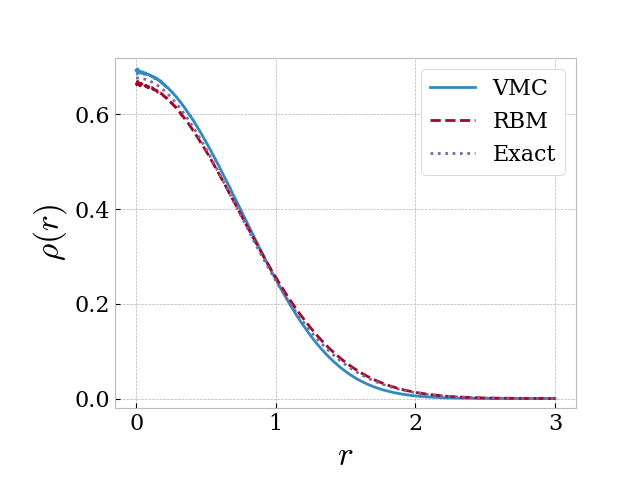
\includegraphics[width=7cm]{../plots/int0/onebody/2D/2P/GD_MC2pow30_w1p0.png}}
	\subfloat[3D]{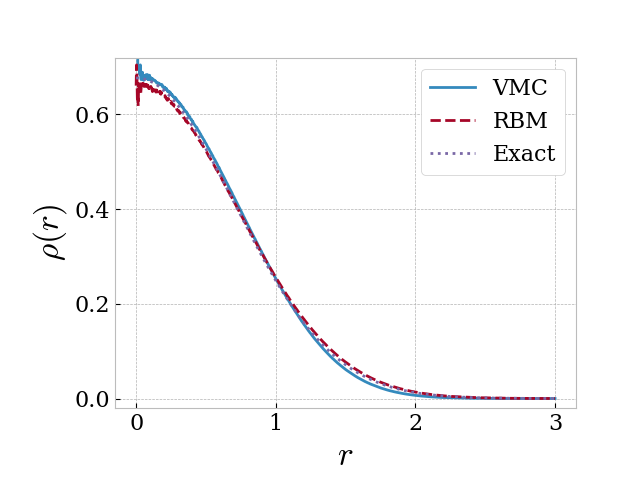
\includegraphics[width=7cm]{../plots/int0/onebody/3D/2P/GD_MC2pow30_w1p0.png}}
	\caption{Plots of the radial one-body density profile for quantum dots with $N=2$ non-interacting electrons and frequency $\omega=1.0$. Both two-dimensional (2D) and three-dimensional (3D) dots are simulated using the VMC and RBM ansätze, and they are compared to the analytical case $\rho(r)\propto\exp(-r^2)$ (Exact). For abbreviations and description of the natural units used, see the text.}
	\label{fig:OB_nointeraction}
\end{figure}

Furthermore, we examine the spatial one-body density and radial two-body density. For the same quantum dot system as above, the density profiles are compared to analytical results in figure \eqref{fig:ED_nointeraction}. For the one-body density plots, we observe that both the RBM and VMC ansätze provide density profiles similar the exact profile. Also the two-body densities match the analytical density profile for both ansätze, but we observe a suspicious cross on the obtained two-body density profiles. This cross occurs since we in practice calculate the density for positive $r_i$ and $r_j$. We then get the density profile presented in the first quadrant of the plots, and simply rotate the same density around origin ($r_i=r_j=0$) to get intuitive and illustrative plots. This also explains the negative values of $r_i$ and $r_j$, which otherwise would not make sense. 

\begin{figure}
	\centering
	\captionsetup[subfigure]{labelformat=empty}
	\subfloat{\raisebox{2.cm}{\rotatebox[origin=t]{90}{one-body}}}\hspace{0.1cm}
	\subfloat{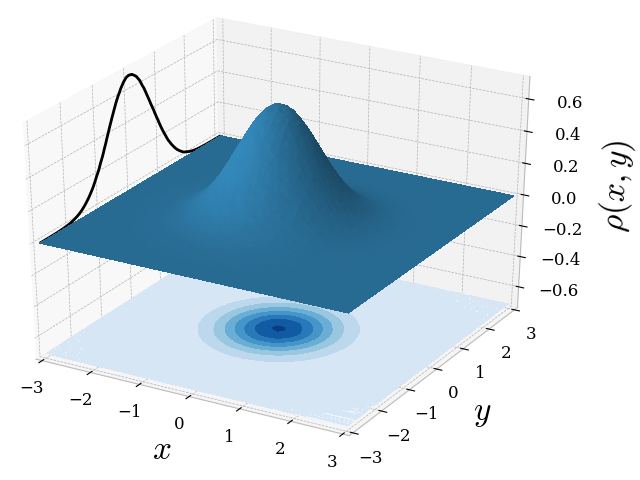
\includegraphics[width=5.1cm]{../plots/int0/onebody2/2D/2P/1.000000w/RBM_ADAM_MC268435456.png}}
	\subfloat{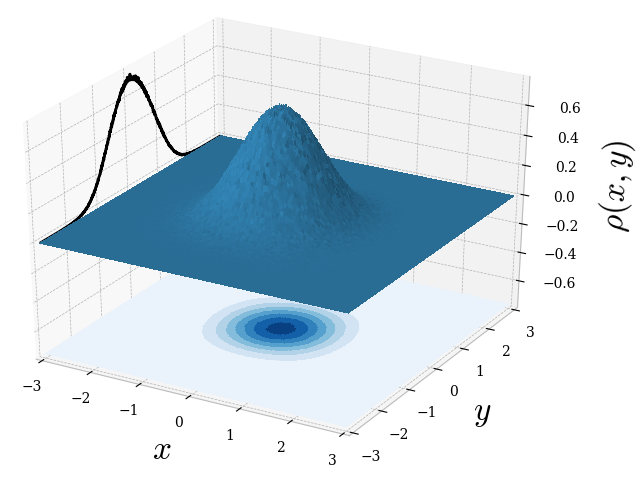
\includegraphics[width=5.1cm]{../plots/int0/onebody2/2D/2P/1.000000w/VMC_GD_MC2pow30_blue_small.png}}
	\subfloat{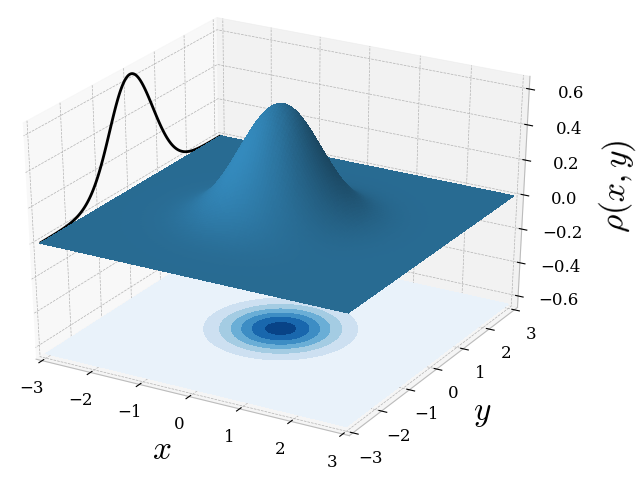
\includegraphics[width=5.1cm]{../plots/int0/onebody2/2D/2P/1.000000w/Exact.png}}
	
	\subfloat{\raisebox{2.cm}{\rotatebox[origin=t]{90}{two-body}}}\hspace{0.1cm}
	\subfloat[RBM]{{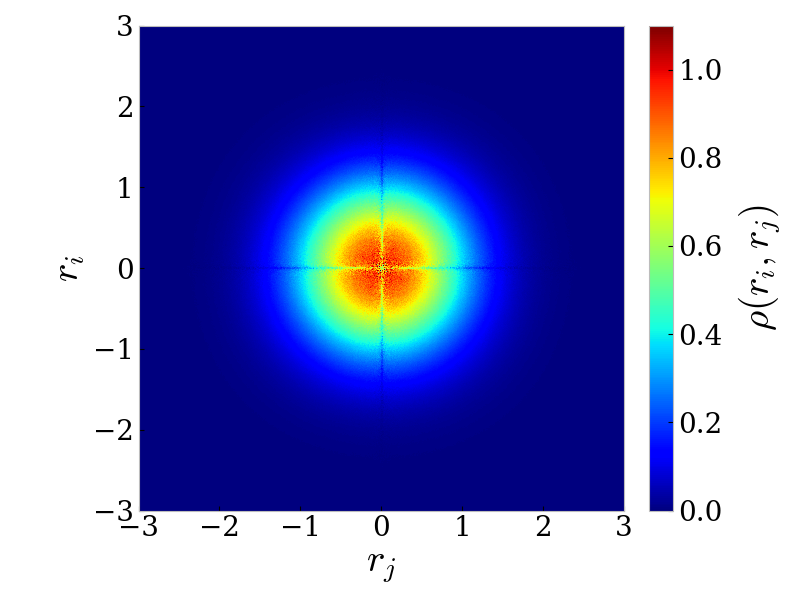
\includegraphics[width=5.1cm]{../plots/int0/twobody/RBM/2D/2P/1.000000w/RBM_GD_MC2pow30.png}}}
	\subfloat[VMC]{{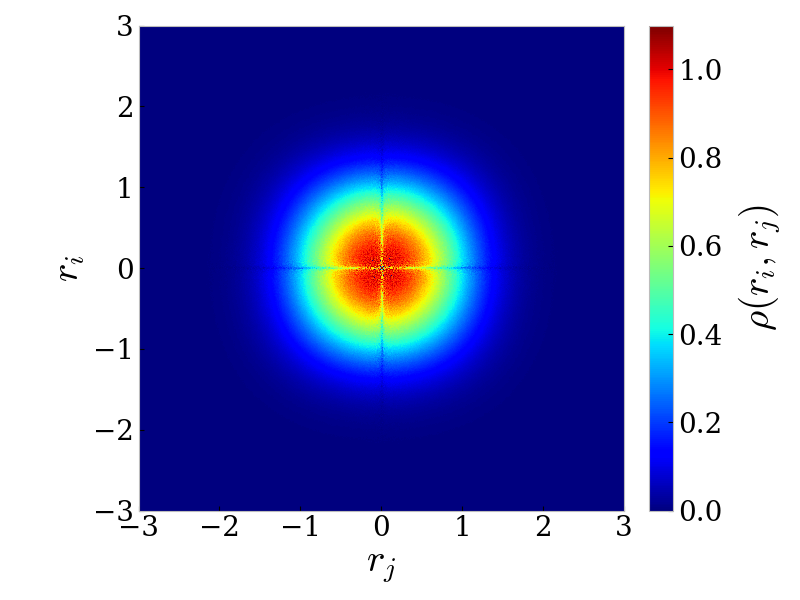
\includegraphics[width=5.1cm]{../plots/int0/twobody/VMC/2D/2P/1.000000w/VMC_GD_MC2pow30.png}}}
	\subfloat[Exact]{{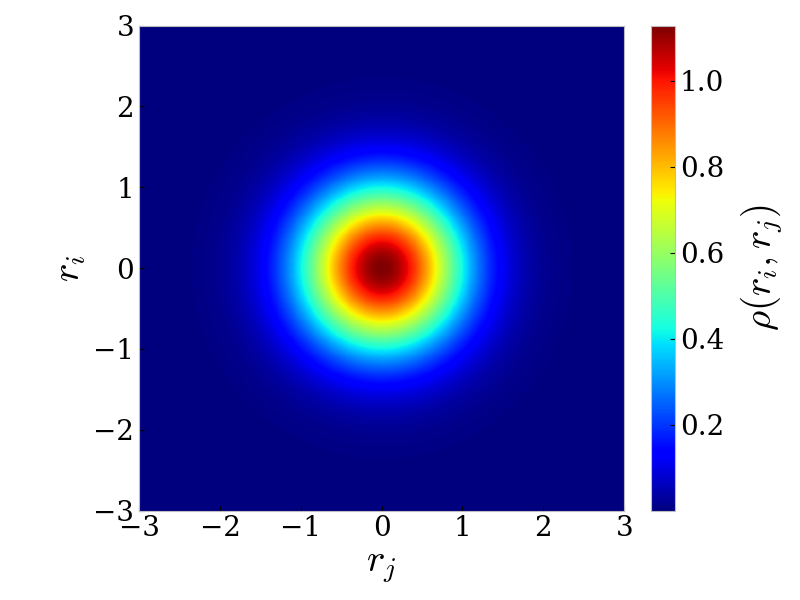
\includegraphics[width=5.1cm]{../plots/int0/twobody/VMC/2D/2P/1.000000w/exact.png}}}
	
	\caption{Plots of the electron density profile, $\rho$, of a two-dimensional quantum dot with $N=2$ non-interacting electrons and frequency $\omega=1.0$. The upper plots are the (spatial) one-body density distribution (one-body), where the surface plot and the contour plot on the $xy$-plane illustrate the density, and the graph on the $yz$-plane represents the cross-section through $x=0$. The lower plots are the radial two-body density distributions (two-body). Besides, we compare the results to the analytical densities (Exact), given by $\rho(x,y)\propto\exp(-x^2-y^2)$ and $\rho(r_i,r_j)\propto\text{exp}(-r_i^2-r_j^2)$, respectively. For  abbreviations and description of the natural units used, see the text.}
	\label{fig:ED_nointeraction}
\end{figure}

As discussed in section \ref{sec:electrondensity}, the electron density should be normalized such that the integral over the density function, $\rho$, corresponds to the number of electrons. \iffalse For the one-body density, this corresponds to $\int dr\rho(r)=N$ for the radial density profile and $\int dxdy\rho(x,y)=N$ for the spatial density distribution and for the two-body radial density profile the normalization condition is $\int dr_idr_j\rho(r_i,r_j)=N$.\fi However, there is no standard way of normalizing these densities when they are calculated using bins, as the normalization constant depends on the number of bins. This is not very important either; we are only interested in the relative densities and the shapes of the density plots. We have been consequent when normalizing the density plots, such that the various density magnitudes can be compared to each other.

\subsection{Atoms}
To further verify the implementation, we address atomic systems with non-interacting electrons. For these systems, the variational Monte Carlo simulations are based on a trial wave function ansatz consisting of a single Slater determinant with the hydrogen-like orbitals as the single-particle functions. In table \eqref{tab:atomswointeraction}, the ground state energy of some selected atoms are listed with the exact energies, given by the Bohr formula presented in equation \eqref{eq:bohrformula}. Besides, we add calculations of the hydrogen ground state energy as another simple validation of the code. It is apparent that the obtained energies are in line with the exact energies, indicating that the code simulates atomic systems correctly.

\begin{table}
	\caption{Ground state energy of neutral atoms with atomic number $Z$ and non-interacting electrons. A single Slater determinant with hydrogen-like orbitals was used as the trial wave function ansatz. The analytical energy (Exact) is obtained by the Bohr formula, $E_n=Z^2/2n^2$. The variance is zero to machine-precision for all listed results. For abbreviations and description of the Hartree atomic units used, see the text.}
	\label{tab:atomswointeraction}
	\begin{tabularx}{\textwidth}{R{3.5cm}lrrR{2.5cm}R{2.5cm}} \hline\hline
		& Atom & $Z$ & \makecell{\\ \phantom{=}} & VMC & Exact \\ \hline \\
		
		& H & 1 && -0.5 & -0.5 \\
		& He & 2 && -4.0 & -4 \\
		& Be & 4 && -20.0 & -20 \\
		& Ne & 10 && -200.0 & -200 \\ \hline\hline
	\end{tabularx}
\end{table}

For completeness, we present the radial one-body density of the helium atom in figure \eqref{fig:helium_nointeraction}. The density is multiplied by $r^2$ as this allows us to clarify the peaks in the one-body density. We see that the produced density curve is more or less identical to the exact density curve, found from the definition in section \ref{eq:onebody_density}.

\begin{figure}[H]
	\centering
	\captionsetup[subfigure]{labelformat=empty}
	\subfloat{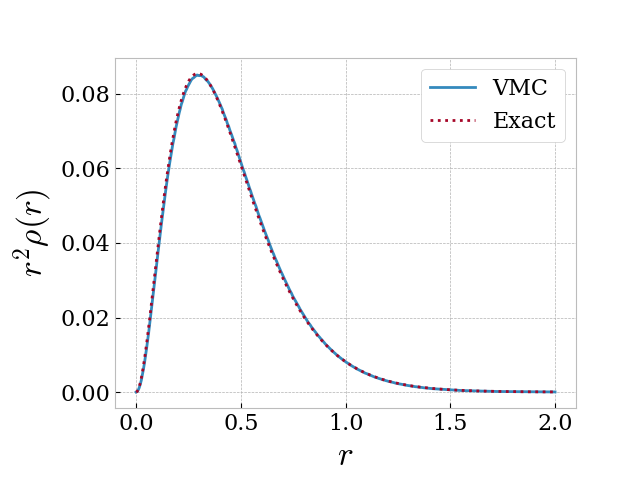
\includegraphics[width=9cm]{../plots/int0/onebody/helium.png}}
	\caption{Plot of the radial one-body density profile for the non-interacting helium atom. A single Slater determinant with hydrogen-like orbitals was used as the trial wave function ansatz. The analytical density (Exact) was obtained by the formula $\rho(r)\propto\exp(-2r)$, and the densities were multiplied with the radius squared. For abbreviations and description of the Hartree atomic units used, see the text.}
	\label{fig:helium_nointeraction}
\end{figure}

\cleardoublepage
\section{Quantum dots} \label{sec:quantumdotresults}
We now move on to the more interesting case with repulsive interaction between the electrons. Analytical results are in general unavailable for this case, apart from a few semi-analytical energies and wave functions for the two- and three-dimensional quantum dots. We will for this system calculate the ground state energy, the one-body density, and the two-body density. 

The simulations depend on an array of hyper-parameters, which need to be reasonable in order to achieve acceptable results. Firstly, the simulations are very sensitive to the learning rate. On one hand, it has to be large enough for the simulation to converge in an adequate number of steps. On the other hand, it needs to be small to avoid the gradients to explode as discussed in chapter \ref{chp:machinelearning}. Appropriate learning rates were found to be in the range $\eta\in\{10^{-5}, 10^{0}\}$, where large systems and/or systems with low frequency required the lowest learning rates. Also, the step length needs to be set cleverly, as we want to sample over the space where the electrons physically can be located in a reasonable number of cycles. For a narrow oscillator potential (high frequency), the step length is typically smaller than for a wide oscillator (low frequency). The acceptance ratio is directly dependent on the step length, where we want a high acceptance ratio to keep the computational cost low. However, we experienced that a too high acceptance ratio is neither favorable, as it makes the simulation diverge. Keeping an acceptance ratio at around 0.995 was found to be optimal, with a step length in the range $\Delta x\in\{10^{-2},10^0\}$. The initial electron and parameter configurations are crucial in order to make the simulations converge rapidly. Furthermore, the statistical error depends on the number of Monte Carlo cycles, where a large number of cycles is preferred as discussed in section \ref{sec:vmc}. 

We have applied an adaptive number of cycles, which means that the number of Monte Carlo cycles per iteration is increased for the last iterations. Firstly, this makes the final energy more accurate due to more statistics. Secondly, we obtain less noisy convergence and density plots with this technique. All results below are produced using $M=2^{20}=1,048,576$ number of cycles per iteration until the energy has converged. Then, we run 10 more iterations with the number of cycles increased to $M=2^{24}=16,777,216$ and for the very last iteration we run $M=2^{28}=268,435,456$ or $M=2^{30}=1,073,741,824$ cycles.

Initially, we look at two-dimensional quantum dots with up to $N=56$ electrons and three-dimensional quantum dots with up to $N=40$ electrons. The frequencies span from  $\omega=0.1$ to $\omega=1.0$. For these systems, we will compute the ground state energy, the one-body density, and the two-body density. After that, we move on to some special cases where the dots have low frequency ($\omega=0.01$) and large dots ($N>56$) to test how far we can go. We also have a thorough discussion of how the energy is distributed between kinetic and potential energy, and compare the kinetic-potential energy ratio to the virial theorem.

\afterpage{
	\begin{landscape}
		\begin{table}
			\captionsetup{width=0.9\hsize}
			\caption{The ground state energy of two-dimensional quantum dots with $N$ electrons and frequency $\omega$. The HF results are taken from \citet{mariadason_quantum_2018}, the DMC results are taken from \citet{hogberget_quantum_2013} and semi-analytical results (Exact) are taken from \citet{taut_two_1994}. The energy is given in units of $\hbar$ (natural units), and the numbers in parenthesis are the statistical uncertainties in the last digit. Empty cells in the table imply that the result is not available. For abbreviations see the text. $*$ For $N=2$ and $\omega=1/6$, the HF result was generated using the code developed by \citet{mariadason_hartreefock_2018}.}
			\begin{tabularx}{\hsize}{llR{2.65cm}R{2.65cm}R{2.65cm}R{2.65cm}R{2.65cm}R{2.65cm}R{2.65cm}} \hline\hline
				\label{tab:quantumdotswinteraction2D1}
				\makecell{\\ $N$ \\ \phantom{=}} & $\omega$ & \multicolumn{1}{c}{RBM} & \multicolumn{1}{c}{RBM+SJ} & \multicolumn{1}{c}{RBM+PJ} & \multicolumn{1}{c}{\makecell{HF \\ (Ref.\cite{mariadason_quantum_2018})}} & \multicolumn{1}{c}{VMC} & \multicolumn{1}{c}{\makecell{DMC \\ (Ref.\cite{hogberget_quantum_2013})}} & \multicolumn{1}{c}{\makecell{Exact \\ (Ref.\cite{taut_two_1994})}} \\ \hline \\
				2 & 0.1 & 0.4728(1) & 0.44856(1) & 0.440975(8) & 0.525635\phantom{$^*$} & 0.44129(1) & 0.44079(1) \\ 
				& 1/6 & 0.7036(1) & 0.67684(7) & 0.66715(6) & 0.768675$^*$ & 0.66710(1) & & 2/3 \\
				& 0.28 & 1.07050(4) & 1.03470(7) & 1.021668(7) & 1.14171\phantom{$^*$} & 1.02192(1) & 1.02164(1) \\
				& 0.5 & 1.72293(7) & 1.67739(9) & 1.659637(6) & 1.79974\phantom{$^*$} & 1.65974(1) & 1.65977(1)  \\
				& 1.0 & 3.0803(2) & 3.02108(5) & 2.999587(5) & 3.16190\phantom{$^*$} & 2.99936(1) & 3.00000(1) & 3.0 \\ 
				\hline \\
				
				6 & 0.1 & 3.697(1) & 3.63825(9) & 3.5700(2) & 3.85238\phantom{$^*$} & 3.5695(1) & 3.55385(5) \\ 
				& 0.28 & 7.9273(9) & 7.7313(2) & 7.6203(2) & 8.01957\phantom{$^*$} & 7.6219(1) & 7.60019(6) \\
				& 0.5 & 12.241(1) & 11.9659(5) & 11.8074(2) & 12.2713\phantom{$^*$} & 11.8104(2) & 11.78484(6) \\
				& 1.0 & 20.716(1) & 20.3393(8) & 20.1832(2) & 20.7192\phantom{$^*$} & 20.1918(2) & 20.15932(8) \\ \hline \\
				
				12 & 0.1 & 12.679(1) & 12.5964(7) & 12.3416(4) & 12.9247\phantom{$^*$} & 12.29962(9) & 12.26984(8) \\ 
				& 0.28 & 26.389(2) & 26.051(1) & 25.7331(5) & 26.5500\phantom{$^*$} & 25.7049(4) & 25.63577(9) \\
				& 0.5 & 40.440(3) & 39.6340(7) & 39.2743(6) & 40.2161\phantom{$^*$} & 39.2421(5) & 39.1596(1) \\
				& 1.0 & 67.632(3) & 66.1898(8) & 65.7911(7) & 66.9113\phantom{$^*$} & 65.7026(4) & 65.7001(1) \\ \hline
			\end{tabularx}
		\end{table}
		
		\begin{table}
			\label{tab:quantumdotswinteraction2D2}
			\begin{tabularx}{\hsize}{llR{2.65cm}R{2.65cm}R{2.65cm}R{2.65cm}R{2.65cm}R{2.65cm}R{2.65cm}} \\
				20 & 0.1 & 30.824(2) & 30.567(3) & 30.1553(9) & 31.1902\phantom{$^*$} & 30.0403(2) & 29.9779(1) \\ 
				& 0.28 & 63.788(4) & 62.786(3) & 62.148(1) & 63.5390\phantom{$^*$} & 62.0755(7) & 61.9268(1) \\
				& 0.5 & 96.410(1) & 94.920(4) & 94.104(1) & 95.7328\phantom{$^*$} & 94.0433(9) & 93.8752(1) \\
				& 1.0 & 159.428(3) & 156.816(4) & 156.104(1) & 158.004\phantom{$^*$} & 155.8900(4) & 155.8822(1) & \phantom{=} \\ 
				\hline \\
				
				30 & 0.1 & 61.829(5) & 61.198(2) & 60.774(2) & & 60.585(1) & 60.4205(2) \\ 
				& 0.28 & 126.958(6) & 125.413(2) & 124.437(2) & & 124.195(2) & 123.9683(2) \\
				& 0.5 & 191.495(7) & 188.995(5) & 187.488(2) & & 187.325(3) & 187.0426(2) \\
				& 1.0 & 315.364(8) & 309.997(6) & 308.989(2) & & 308.576(1) & 308.5627(2) \\ \hline \\
				
				42 & 0.1 & 109.892(6) & 109.48(2) & 108.183(1) & &  107.928(2) & 107.6389(2) \\ 
				& 0.28 & 224.462(8) & 224.184(9) & 222.200(5) & & 220.224(2) & 219.8426(2) \\
				& 0.5 & 337.523(8) & 333.582(9) & 331.410(3) & & 331.276(3) & 330.6306(2) \\
				& 1.0 & 553.40(1) & 545.817(9) & 543.746(3) & & 542.977(2) & 542.9428(8) \\ \hline \\
				
				56 & 0.1 & 179.789(6) & 179.59(1) & 178.501(5) & & 176.774(3) & 175.9553(7) \\ 
				& 0.28 & 364.85(1) & 364.165(9) & 359.83(2) & & 359.63(1) & 358.145(2) \\
				& 0.5 & 547.46(1) & 545.74(1) & 538.810(7) & & 538.686(9) & 537.353(2) \\
				& 1.0 & 894.12(2) & 882.93(1) & 881.010(5) & & 879.514(3) & 879.3986(6) \\ \hline\hline
			\end{tabularx}
		\end{table}
		
		\begin{table}
			\captionsetup{width=0.9\hsize}
			\caption{The ground state energy of three-dimensional quantum dots with $N$ electrons and frequency $\omega$.  The HF results are taken from \citet{mariadason_quantum_2018}, the DMC results are taken from \citet{hogberget_quantum_2013} and semi-analytical results (Exact) are taken from \citet{taut_two_1993}. The energy is given in units of $\hbar$ (natural units), and the numbers in parenthesis are the statistical uncertainties in the last digit. Empty cells in the table imply that the result is not available. For abbreviations see the text.} 
			\begin{tabularx}{\hsize}{llR{2.65cm}R{2.65cm}R{2.65cm}R{2.65cm}R{2.65cm}R{2.65cm}R{2.65cm}} \hline\hline
				\label{tab:quantumdotswinteraction3D1}
				\makecell{\\ $N$ \\ \phantom{=}} & $\omega$ & \multicolumn{1}{c}{RBM} & \multicolumn{1}{c}{RBM+SJ} & \multicolumn{1}{c}{RBM+PJ} & \multicolumn{1}{c}{\makecell{HF \\ (Ref.\cite{mariadason_quantum_2018})}} & \multicolumn{1}{c}{VMC} & \multicolumn{1}{c}{\makecell{DMC \\ (Ref.\cite{hogberget_quantum_2013})}} & \multicolumn{1}{c}{\makecell{Exact \\ (Ref.\cite{taut_two_1993})}} \\ \hline \\
				2 & 0.1 & 0.5177(1) & 0.50214(3) & 0.500080(6) & 0.529065 & 0.500083(7) & 0.499997(3) & 0.5 \\
				& 0.28 & 1.2261(1) & 1.20475(4) & 1.201710(6) & 1.23722 & 1.201752(6) & 1.201725(2) \\
				& 0.5 & 2.0269(1) & 2.00371(4) & 1.999912(5) & 2.03851 & 1.999977(5) & 2.000000(2) & 2.0 \\
				& 1.0 & 3.7574(1) & 3.73543(4) & 3.729827(5) & 3.77157 & 3.730030(5) & 3.730123(3) \\ 
				\hline \\
				
				8 & 0.1 & 5.8910(6) & 5.7498(4) & 5.718(4) & 5.86255 & 5.7126(1) & 5.7028(1) \\ 
				& 0.28 & 12.650(1) & 12.2492(4) & 12.2056(2) & 12.3987 & 12.2050(2) & 12.1927(1) \\
				& 0.5 & 19.487(2) & 19.0241(4) & 18.9747(2) & 19.1916 & 18.9759(1) & 18.9611(1) \\
				& 1.0 & 33.302(1) & 32.7159(6) & 32.6820(2) & 32.9246 & 32.6863(2) & 32.6680(1) \\ 
				\hline \\
				
				20 & 0.1 & 27.813(2) & 27.470(1) & 27.3382(8) & & 27.3144(5) & 27.2717(2) \\ 
				& 0.28 & 57.700(4) & 56.600(1) & 56.4477(6) & & 56.4297(5) & 56.3868(2) \\
				& 0.5 & 87.840(4) & 85.893(1) & 85.7153(6) & & 85.7161(5) & 85.6555(2) \\
				& 1.0 & 146.292(4) & 143.209(2) & 142.9409(6) & & 142.9560(7) & 142.8875(2) \\ \hline \\
				
				40 & 0.1 & 89.45(8) & 89.618(4) & 88.596(4) & & 88.182(1) \\ 
				& 0.28 & 182.714(6) & 181.877(4) & 179.630(1) & & 179.567(1) \\
				& 0.5 & 275.262(7) & 271.030(4) & 269.782(2) & & 269.746(1) \\
				& 1.0 & 452.732(8) & 442.874(4) & 442.630(1) & & 442.602(2) \\ \hline\hline
			\end{tabularx}
		\end{table}
	\end{landscape}
}

\subsection{Ground state energy} \label{sec:groundstateenergy}
The ground state energy is a natural starting point as the simulations are based on energy minimization. Moreover, the energy can easily be compared to benchmarks. By exploiting the symmetry of quantum dots with $n=2$ electrons, \citeauthor{taut_two_1993} was able to obtain semi-analytical energies for quantum dots of certain frequencies $\omega$. For two-dimensional dots, he found the energy to be $E=3$ for the frequency $\omega=1$ and $E=2/3$ with $\omega=1/6$ as the frequency \supercite{taut_two_1993}. Additionally, his studies of three-dimensional dots revealed the energy $E=2$ for the frequency $\omega=1/2$ and $E=1/2$ with $\omega=1/10$ as the frequency \supercite{taut_two_1994}. For other references we need to rely on earlier research, usually other simulations. Since diffusion Monte Carlo (DMC) simulations are known to give very accurate results, we will mainly compare our results to the DMC computations by \citet{hogberget_quantum_2013}. These results exist for quantum dots with up to $N=56$ electrons in two dimensions and with up to $N=20$ electrons in three dimensions. Another important reference is the Hartree-Fock (HF) limit, as the HF method approximates the electron-electron correlations by a mean-field. This is a particular interesting reference for simulations with the RBM ansatz, as both the methods approximate the many-body wave function with a single Slater determinant only. Practically, RBM should give a lower energy than the HF limit as the latter is known to be computationally cheap. We use the HF computations from \citet{mariadason_quantum_2018} for two-dimensional quantum dots with up to $N=20$ electrons and three-dimensional quantum dots with up to $N=8$ electrons. For the two-dimensional quantum dot with $N=2$ and frequency $\omega=1/6$, we obtained the HF energy using the code developed by \citet{mariadason_hartreefock_2018}.

Ground state energy computations of two- and three dimensional quantum dots are found in tables \eqref{tab:quantumdotswinteraction2D1} and \eqref{tab:quantumdotswinteraction3D1}, respectively. They are computed using the RBM, RBM+SJ, RBM+PJ and VMC ansätze, and the HF limit and DMC are present for reference purposes. The analytical values are found in the last column. We observe that the ansatz that requires least physical intuition is used, RBM, is the one that gives the highest energies among the ansätze. This is expected as no Jastrow factor is added to account for the correlations. 

For small quantum dots ($N<8$), the RBM ansatz provides a lower energy than the HF limit, and for low frequencies ($\omega<0.5$) the obtained energy is generally also lower. This indicates that simulations with the RBM ansatz is better at modeling the correlations compared to the HF method. Nevertheless, for higher frequencies and larger dots, the HF limit is lower than the energy obtained using the RBM ansatz. When we add more intuition to the trial wave function ansatz in the form of a simple Jastrow factor (RBM+SJ), the energy drops significantly, especially for high frequencies. It is, therefore, lower than the HF limit for all simulations, and surprisingly close to the reference considering the simple form of the Jastrow factor. The statistical errors of RBM+SJ is in general smaller than for RBM, which is a good indication that the method provides a better ground state estimate as the actual ground state obeys a zero-variance property \supercite{assaraf_zero-variance_2003}. 

Furthermore, we add a more complex Jastrow factor in the form of a Padé-Jastrow factor to the RBM ansatz, and we observe that the energy drops further. The RBM+PJ ansatz provides energies entirely on par with VMC, in many cases even lower. Notably, RBM+PJ provides the lowest energies among our implemented methods for dots with $N=2$ electrons, and the statistical errors are also the lowest. This hints that RBM+PJ can obtain a better ground state estimate than VMC for the smallest dots. However, for large dots, RBM+PJ provides slightly higher energies than VMC. We speculate that this might be due to the large number of variational parameters residing in the trial wave function, resulting in a too complex model for the problem. If we recall that the number of hidden units is set to the number of electrons, the number of variational parameters increases rapidly as the number of electrons increases. 

A further novel finding is that all the methods and ansätze provide energies closer to the reference energy in three dimensions compared to two dimensions. For three-dimensional dots, we have a phase space of higher dimensionality than for two-dimensional dots, allowing a larger set of particle configurations. Obtaining an adequate estimate of the ground state energy is therefore more accessible in three dimensions compared to two dimensions.

\begin{figure}
	\centering
	\captionsetup[subfigure]{labelformat=empty}
	\subfloat{\raisebox{2.5cm}{\rotatebox[origin=t]{90}{$N=2$}}}\hspace{0.1cm}
	\subfloat{{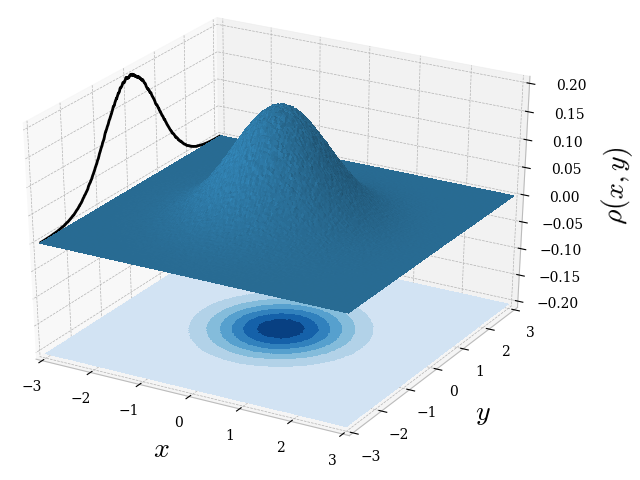
\includegraphics[width=7.8cm]{../plots/int1/onebody2/2D/2P/1.000000w/RBM_ADAM_MC2pow28_smooth_blue.png}}}\hspace{-0.0cm}
	\subfloat{{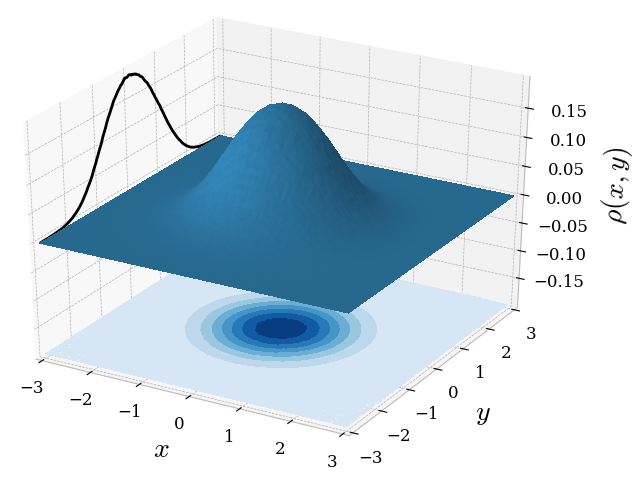
\includegraphics[width=7.8cm]{../plots/int1/onebody2/2D/2P/1.000000w/VMC_ADAM_MC2pow28_smooth_blue.png}}}\\
	
	\subfloat{\raisebox{2.5cm}{\rotatebox[origin=t]{90}{$N=6$}}}\hspace{0.05cm}
	\subfloat{{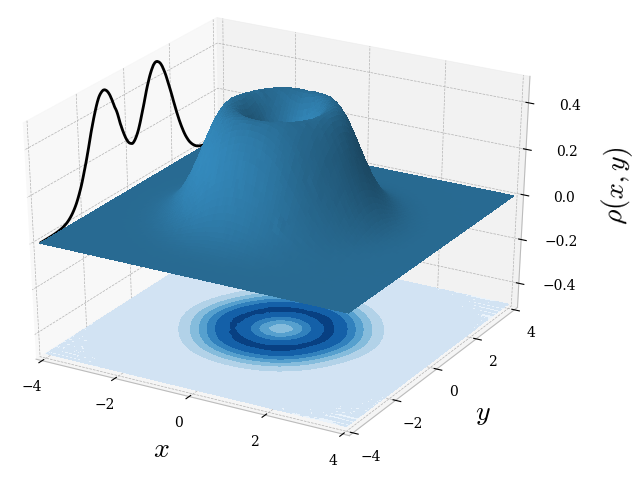
\includegraphics[width=7.8cm]{../plots/int1/onebody2/2D/6P/1.000000w/RBM_ADAM_MC2pow28_smooth_blue.png}}}\hspace{-0.0cm}
	\subfloat{{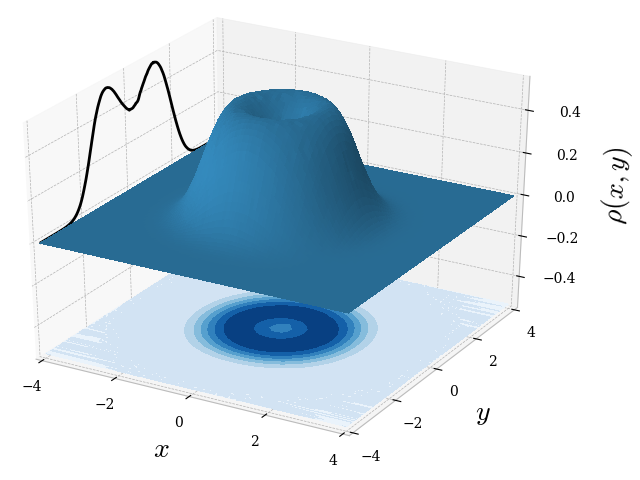
\includegraphics[width=7.8cm]{../plots/int1/onebody2/2D/6P/1.000000w/VMC_ADAM_MC2pow28_smooth_blue.png}}}\\
	
	\subfloat{\raisebox{2.5cm}{\rotatebox[origin=t]{90}{$N=12$}}}\hspace{0.1cm}
	\subfloat[RBM]{{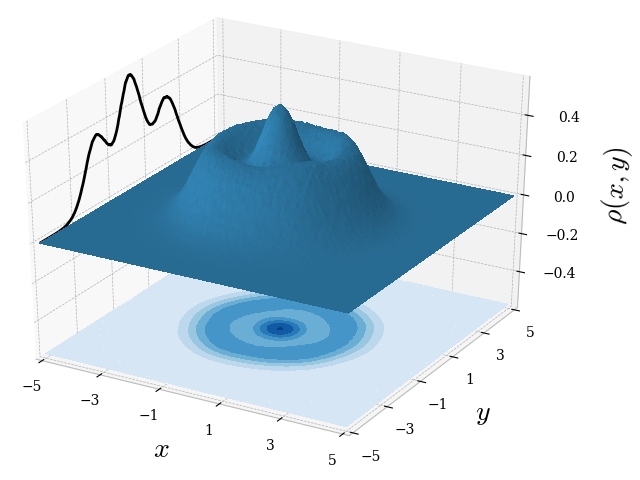
\includegraphics[width=7.8cm]{../plots/int1/onebody2/2D/12P/1.000000w/RBM_ADAM_MC2pow28_smooth_blue.png}}}\hspace{-0.0cm}
	\subfloat[VMC]{{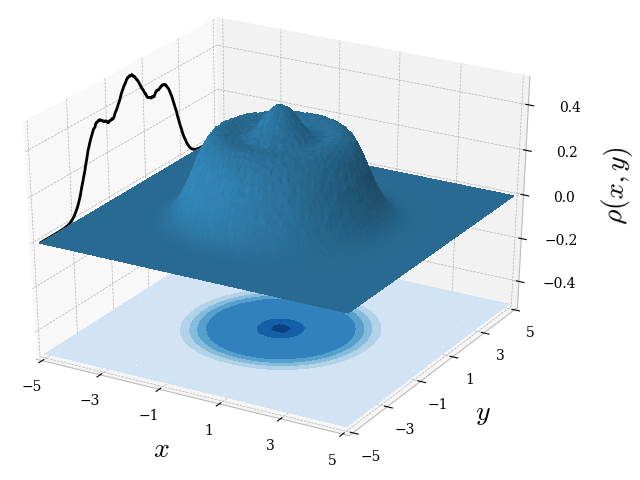
\includegraphics[width=7.8cm]{../plots/int1/onebody2/2D/12P/1.000000w/VMC_ADAM_MC2pow28_smooth_blue.png}}}
	
	\caption{Plots of the one-body density profiles, $\rho(x,y)$, for two-dimensional quantum dots with frequency $\omega=1.0$ and $N=2$, 6 and 12 electrons seen from the top. The surface plot and the contour plot on the $xy$-plane illustrate the density, and the graph on the $yz$-plane represents the cross-section through $x=0$. They were obtained using RBM (left column) and VMC (right column), with the ADAM optimizer and $M=2^{30}=1,073,741,824$ Monte Carlo cycles after convergence. The plots are noise-reduced using a Savitzky-Golay filter. For abbreviations and description of the natural units used, see the text.}
	\label{fig:OB_interaction_1p0w1}
\end{figure}
\begin{figure}
	\centering
	\captionsetup[subfigure]{labelformat=empty}
	\subfloat{\raisebox{2.5cm}{\rotatebox[origin=t]{90}{$N=20$}}}\hspace{0.1cm}
	\subfloat{{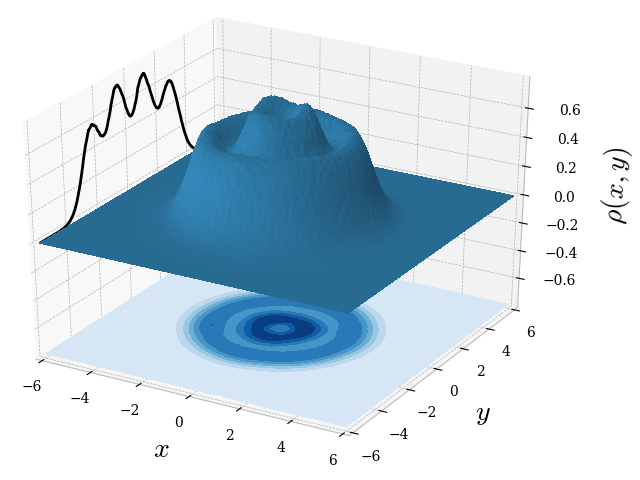
\includegraphics[width=7.8cm]{../plots/int1/onebody2/2D/20P/1.000000w/RBM_ADAM_MC2pow28_smooth_blue.png}}}\hspace{-0.0cm}
	\subfloat{{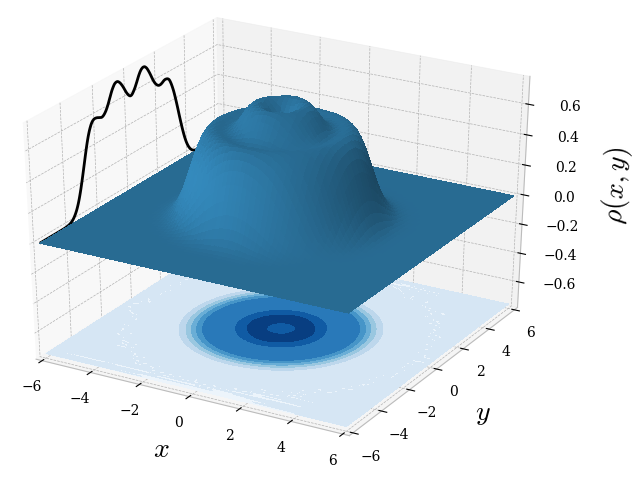
\includegraphics[width=7.8cm]{../plots/int1/onebody2/2D/20P/1.000000w/VMC_ADAM_MC2pow28_smooth_blue.png}}}\\
	
	\subfloat{\raisebox{2.5cm}{\rotatebox[origin=t]{90}{$N=30$}}}\hspace{0.1cm}
	\subfloat{{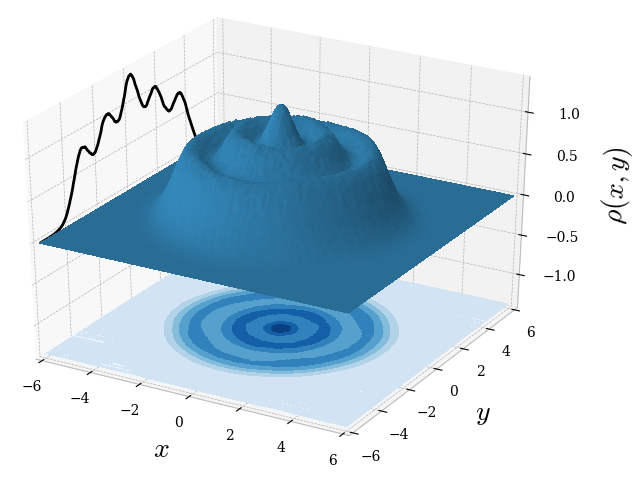
\includegraphics[width=7.8cm]{../plots/int1/onebody2/2D/30P/1.000000w/RBM_ADAM_MC2pow28_smooth_blue.png}}}\hspace{-0.0cm}
	\subfloat{{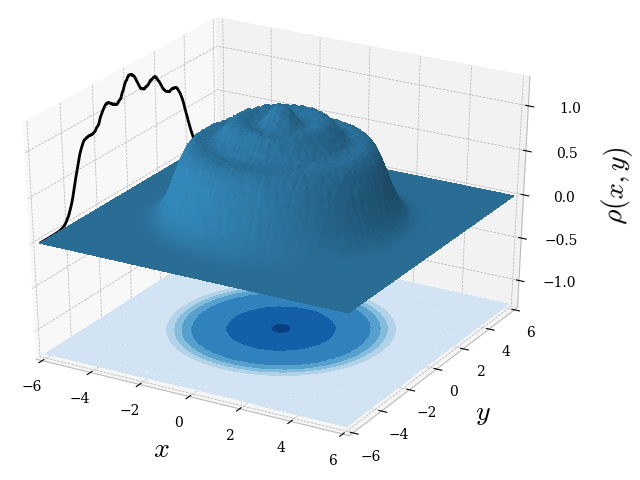
\includegraphics[width=7.8cm]{../plots/int1/onebody2/2D/30P/1.000000w/VMC_ADAM_MC2pow28_smooth_blue.png}}}\\
	
	\subfloat{\raisebox{2.5cm}{\rotatebox[origin=t]{90}{$N=42$}}}\hspace{0.1cm}
	\subfloat[RBM]{{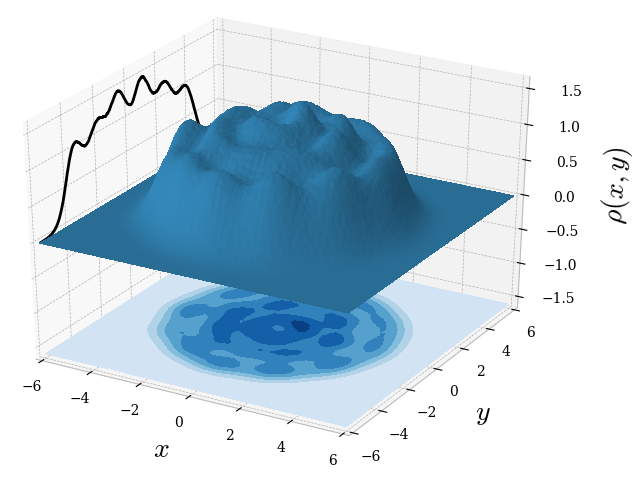
\includegraphics[width=7.8cm]{../plots/int1/onebody2/2D/42P/1.000000w/RBM_ADAM_MC2pow28_smooth_blue.png}}}\hspace{-0.0cm}
	\subfloat[VMC]{{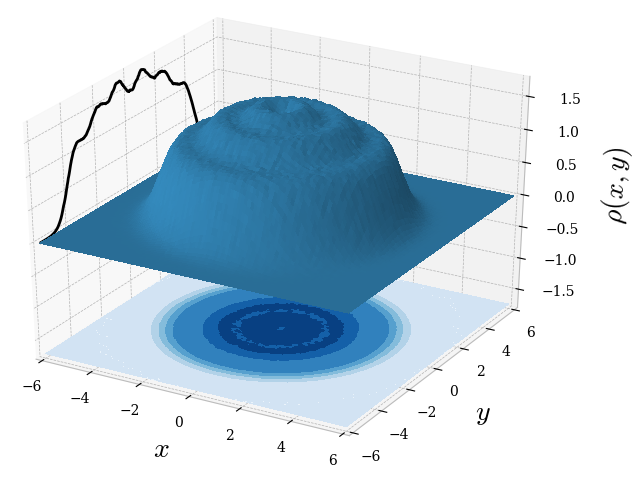
\includegraphics[width=7.8cm]{../plots/int1/onebody2/2D/42P/1.000000w/VMC_ADAM_MC2pow28_smooth_blue.png}}}
	
	\caption{Plots of the one-body density profiles, $\rho(x,y)$, for two-dimensional quantum dots with frequency $\omega=1.0$ and $N=20$, 30 and 42 electrons seen from the top. The surface plot and the contour plot on the $xy$-plane illustrate the density, and the graph on the $yz$-plane represents the cross-section through $x=0$. They were obtained using RBM (left column) and VMC (right column), with the ADAM optimizer and $M=2^{30}=1,073,741,824$ Monte Carlo cycles after convergence. The plots are noise-reduced using a Savitzky-Golay filter. For abbreviations and description of the natural units used, see the text.}
	\label{fig:OB_interaction_1p0w2}
\end{figure}

\subsection{One-body density} \label{sec:onebodyresults}
Another quantity of particular interest is the one-body density. For all the systems presented in tables \eqref{tab:quantumdotswinteraction2D1} and \eqref{tab:quantumdotswinteraction3D1} we have also calculated the one-body density. However, since this results in a large number of plots, the total collection is moved to appendix \ref{chp:totalresults}. Instead, we present the (arguably) most interesting plots of the one-body density here. 

We have computed the one-body density in two different ways: The radial one-body density profile is obtained by dividing the space into plural annuluses, as discussed in section \ref{sec:electrondensityimplementation}. The spatial one-body density profile is obtained by dividing the space into a grid of equally sized bins and counting the number of times an electrons occurs in each bin. The radial density is computationally beneficial as the density typically is stored in $n$ bins compared to $n^2$ bins for the second method, while the spatial density profile can clearly store more information. The spatial profile thereby gives more informative plots, but a radial profile is more convenient when we want to compare multiple ansätze. In other words, there are advantages and disadvantages associated with both methods, and we will, therefore, present both to give an as comprehensive description of the results as possible. 

Initially, we will present the spatial density profiles of two-dimensional quantum dots with frequency $\omega=1.0$. In figure \eqref{fig:OB_interaction_1p0w1} and \eqref{fig:OB_interaction_1p0w2}, the evolution of the one-body density for dots of sizes $N=2$, 6, 12, 20, 30 and 42 are presented, produced using the RBM and VMC trial wave function ansätze. To maximize the amount of information in the plots, we have included a graph presenting the cross-section through $x=0$ on the $yz$-plane and a contour plot of the density on the $xy$-plane, in addition to a 3D surface plot of the density. We observe that the density profile is smooth, with more peaks as the number of electrons increases, representing high densities. For an odd number of shells ($N=2$, 12 and 30) the density has its maximum at the center of the dot, resulting in equal shapes where for example the shape of $N=12$ is seen as the top of $N=30$. On the other hand, for an even number of shells ($N=6$, 20 and 42) the highest density is found at a ridge that encircles the center. Also here the shape of for example $N=20$ is seen as the top of $N=42$. It is apparent that these are the configurations that minimize the energy, with a structure following directly from the Pauli principle, as the electrons are forced to distribute over multiple shells. We have seen that even when we remove the electron-electron interaction, we get the same characteristic wave shape, though narrower. The RBM ansatz provides sharper and more distinct peaks than the VMC ansatz, but the extrema seem to be located at the same radii. These differences may be caused by the way the ansätze model the correlations, where VMC employs the Padé-Jastrow factor and RBM needs to find the best way to account for the correlations itself. 

To connect the observations to something everyone is familiar with, we can draw parallels between the density plots and water ripples. \citet{hogberget_quantum_2013} discusses this in his work, and his plots of the one-body density are consistent with what we have obtained. However, for $N=42$ the RBM ansatz provides a density profile that has ripples in both radial and angular direction, indicating that the simulation has not fully converged to the minimum. This may be an effect of the large number of variational parameters in the trial wave function. Plots of the one-body density profile for the same systems using RBM+SJ and RBM+PJ were generated, but in order to limit us to a few plots we decided move the others in appendix \ref{chp:totalresults}.

In figure \eqref{fig:OB_interaction_23D}, we stick to the frequency $\omega=1.0$ for small two- and three-dimensional quantum dots and compare the results obtained by the VMC, RBM, RBM+SJ, and RBM+PJ ansätze. We investigate dots with $N=2$, 6 and 12 in two dimensions and $N=2$, 8 and 20 in three dimensions. This corresponds to one shell ($S=1$), two shells ($S=2$) and three shells ($S=3$), respectively. For all the numbers of shells, we immediately see that the density plots are similar for two- and three-dimensional dots. The same phenomenon was observed for quantum dots with non-interacting electrons in figure \eqref{fig:OB_nointeraction}, where we argued that the wave function is trivially separable. However, this is not the situation when we look at the interacting case, and it was therefore not obvious to us that the same phenomenon would occur here. Physically, this means that the electrons configure in the same way in three dimensions as in two dimensions, where the average distance from a shell to the center of the dot is dimensionless. Besides the physics, we are also interested in analyzing the performance of the various ansätze. We observe that they all give similar radial density profiles, but the RBM ansatz stands out. Apparently, RBM tends to exaggerate the peaks discussed above and gives a more wavy density plot, as also observed in figures \eqref{fig:OB_interaction_1p0w1} and \eqref{fig:OB_interaction_1p0w2}. Further, RBM+SJ provides results similar to VMC and RBM+PJ. This is consistent with the energy analysis in section \ref{sec:groundstateenergy}, where we found VMC and
\begin{figure}[H]
	\centering
	\captionsetup[subfigure]{labelformat=empty}
	\subfloat{\raisebox{1.5cm}{\rotatebox[origin=t]{90}{$S=1$}}}\hspace{0.1cm}
	\subfloat{{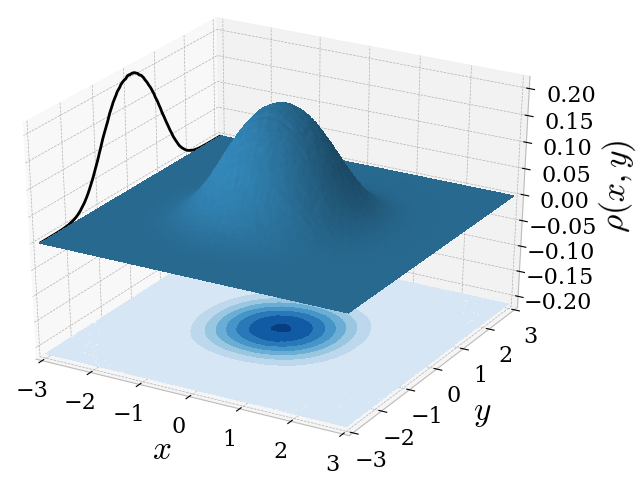
\includegraphics[width=5.1cm]{../plots/int1/onebody2/2D/2P/1.000000w/VMC_ADAM_MC2pow28_smooth_blue_small.png}}}\hspace{-0.0cm}
	\subfloat{{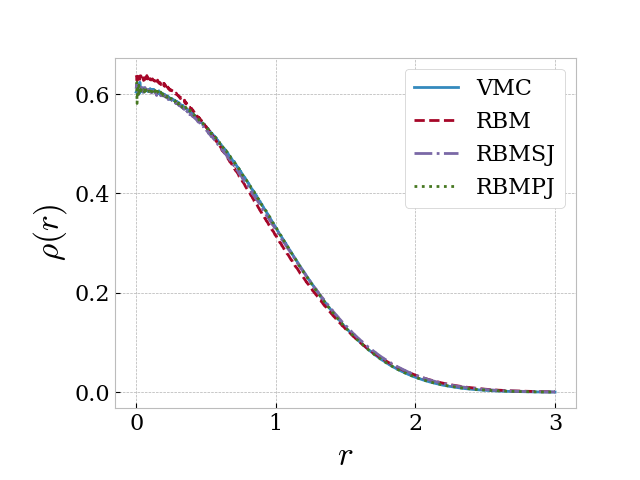
\includegraphics[width=5.1cm]{../plots/int1/onebody/2D/2P/1.000000w/ADAM_MC1048576.png}}}\hspace{-0.5cm}
	\subfloat{{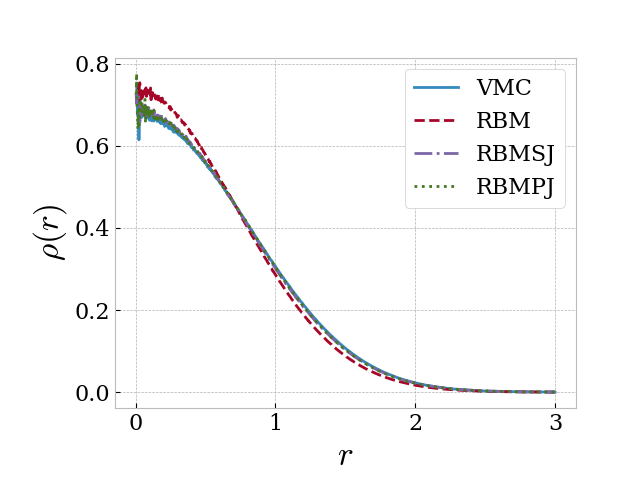
\includegraphics[width=5.1cm]{../plots/int1/onebody/3D/2P/1.000000w/ADAM_MC1048576.png}}}\\ [-0.2cm]
	
	\subfloat{\raisebox{1.5cm}{\rotatebox[origin=t]{90}{$S=2$}}}\hspace{0.1cm}
	\subfloat{{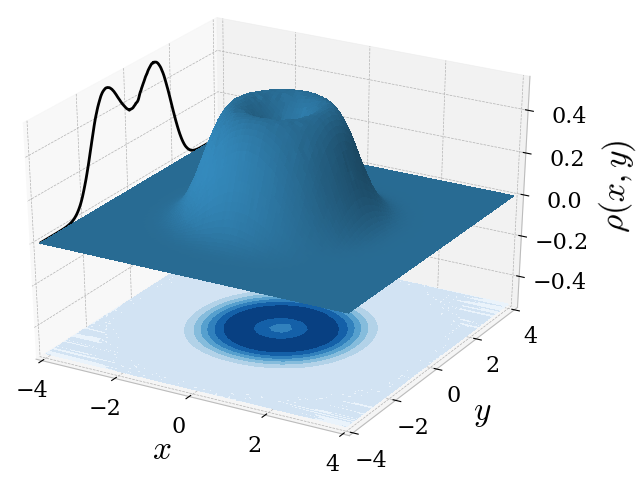
\includegraphics[width=5.1cm]{../plots/int1/onebody2/2D/6P/1.000000w/VMC_ADAM_MC2pow28_smooth_blue_small.png}}}\hspace{-0.0cm}
	\subfloat{{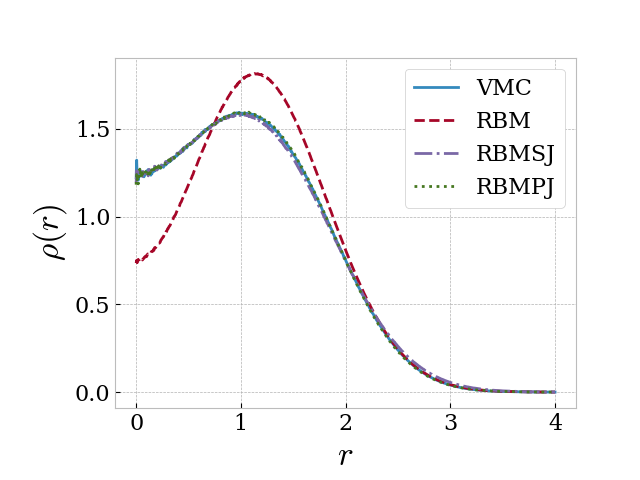
\includegraphics[width=5.1cm]{../plots/int1/onebody/2D/6P/1.000000w/ADAM_MC1048576.png}}}\hspace{-0.5cm}
	\subfloat{{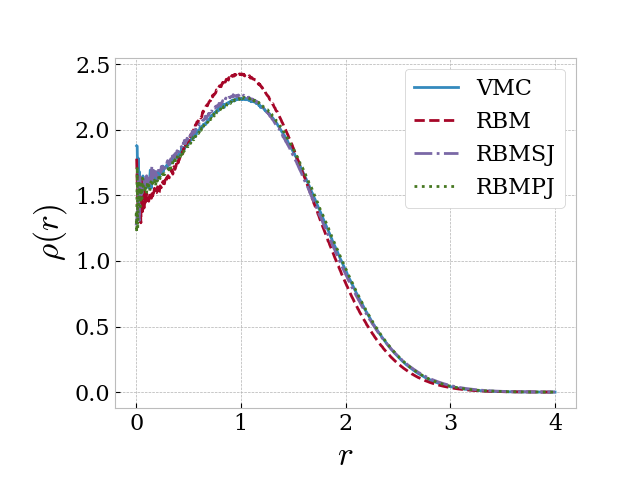
\includegraphics[width=5.1cm]{../plots/int1/onebody/3D/8P/1.000000w/ADAM_MC1048576.png}}}\\ [-0.2cm]
	
	\subfloat{\raisebox{1.5cm}{\rotatebox[origin=t]{90}{$S=3$}}}\hspace{0.1cm}
	\subfloat[VMC, 2D]{{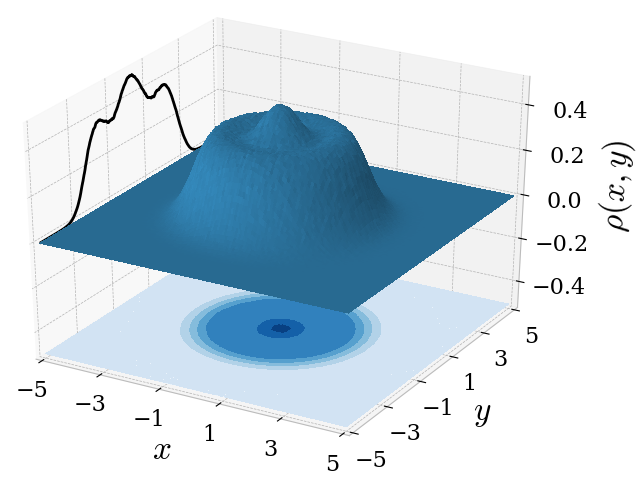
\includegraphics[width=5.1cm]{../plots/int1/onebody2/2D/12P/1.000000w/VMC_ADAM_MC2pow28_smooth_blue_small.png}}}\hspace{-0.0cm}
	\subfloat[2D]{{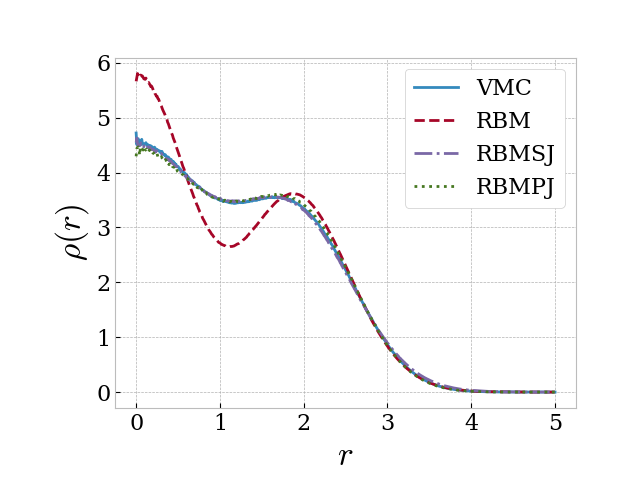
\includegraphics[width=5.1cm]{../plots/int1/onebody/2D/12P/1.000000w/ADAM_MC1048576.png}}}\hspace{-0.5cm}
	\subfloat[3D]{{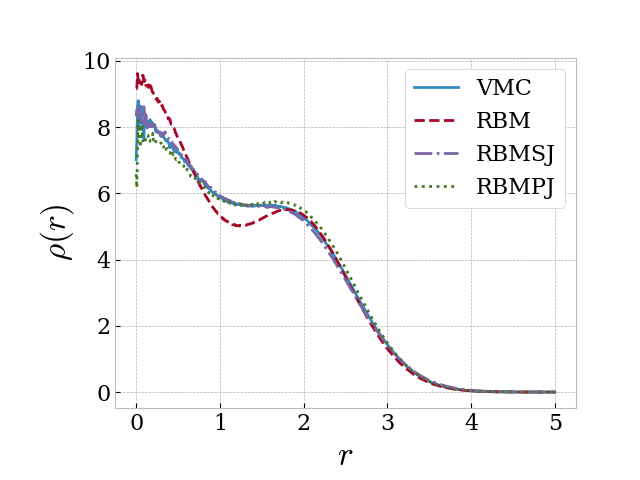
\includegraphics[width=5.1cm]{../plots/int1/onebody/3D/20P/1.000000w/ADAM_MC1048576.png}}}
	
	\caption{Plots of the one-body density profile, $\rho$, for small quantum dots with frequency $\omega=1.0$. We look at the three lowest shells $S=1$, 2 and 3 seen from the top, corresponding to $N=2$, 6, and 12 electrons in two dimensions (2D) and $N=2$, 8 and 20 electrons in three dimensions (3D). In the first column, the surface plot and the contour plot on the $xy$-plane illustrate the density and the graph on the $yz$-plane represents the cross-section through $x=0$. In the middle column, the corresponding radial density profiles are obtained using RBM, RBM+SJ, RBM+PJ and VMC. In the last column, the radial density profiles for the three-dimensional dots are given using the same methods. ADAM optimizer was used, and after convergence, the number of Monte Carlo cycles was $M=2^{30}=1,073,741,824$. The surface plots are noise-reduced using a Savitzky-Golay filter. For  abbreviations and description of the natural units used, see the text.}
	\label{fig:OB_interaction_23D}
\end{figure}
\noindent
RBM+PJ to be the most accurate ansätze, followed by RBM+SJ and RBM in that order. We also observe some noise close to $r=0$, which is caused by the fact that the number of Monte Carlo cycles is finite and we in practice have bins of different sizes.

\begin{figure}
	\centering
	\captionsetup[subfigure]{labelformat=empty}
	\subfloat{\raisebox{3cm}{\rotatebox[origin=t]{90}{$\omega=0.1$}}}\hspace{0.1cm}
	\subfloat{{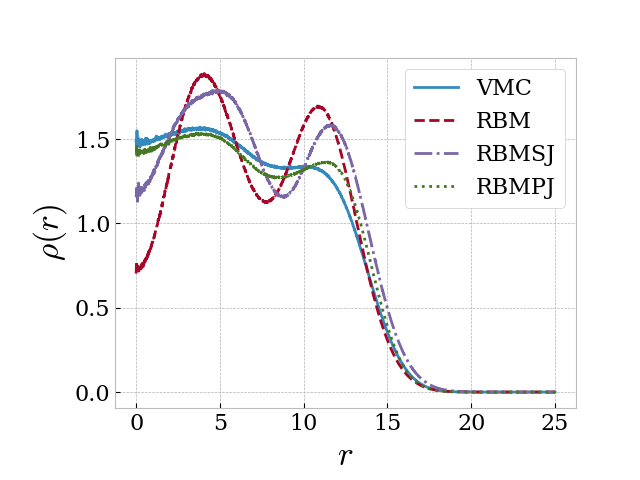
\includegraphics[width=8cm]{../plots/int1/onebody/2D/20P/0.100000w/ADAM_MC1048576.png}}}\hspace{-0.5cm}
	\subfloat{{\includegraphics[width=8cm]{../plots/int1/onebody/2D/42P/0.100000w/ADAM_MC1048576.png}}}\\
	
	\subfloat{\raisebox{3cm}{\rotatebox[origin=t]{90}{$\omega=0.5$}}}\hspace{0.1cm}
	\subfloat{{\includegraphics[width=8cm]{../plots/int1/onebody/2D/20P/0.500000w/ADAM_MC1048576.png}}}\hspace{-0.5cm}
	\subfloat{{\includegraphics[width=8cm]{../plots/int1/onebody/2D/42P/0.500000w/ADAM_MC1048576.png}}}\\
	
	\subfloat{\raisebox{3cm}{\rotatebox[origin=t]{90}{$\omega=1.0$}}}\hspace{0.1cm}
	\subfloat[20P]{{\includegraphics[width=8cm]{../plots/int1/onebody/2D/20P/1.000000w/ADAM_MC1048576.png}}}\hspace{-0.5cm}
	\subfloat[42P]{{\includegraphics[width=8cm]{../plots/int1/onebody/2D/42P/1.000000w/ADAM_MC1048576.png}}}
	
	\caption{Plots of the one-body density profiles, $\rho(r)$, for two-dimensional quantum dots with $N=20$ (left column) and $N=42$ (right column) and oscillator frequencies $\omega=0.1$, 0.5 and 1.0 seen from the top. The ADAM optimizer was used, and after convergence the number of Monte Carlo cycles was $M=2^{28}=268,435,456$. For  abbreviations and description of the natural units used, see the text.}
	\label{fig:OB_interaction}
\end{figure}

We now move on to larger two-dimensional dots and frequencies lower than $\omega=1.0$ to see if the observed behavior is conserved also when the correlations get stronger. In figure \eqref{fig:OB_interaction}, we plot the radial density profile for two-dimensional quantum dots with $N=20$ and 42, and frequencies $\omega=0.1$, 0.5 and 1.0. The results demonstrate that the peaks discussed above are conserved for lower frequencies, and their shapes change slightly as the frequency drops. Also, the density distribution is spatially expanded as the frequency drops, since the force pushing the electrons towards the center of the dot gets weaker. For high frequencies, the VMC, RBM+PJ, and RBM+SJ ansätze appear to give similar density plots. When lowering the frequency, the difference gets gradually more visible. In particular, the peaks for frequency $\omega=0.1$ do no longer match for the various ansätze. Especially, RBM and RBM+SJ differ from VMC and RBM+PJ, indicating that the final results are heavily dependent on the way the ansatz account for the correlations. RBM+SJ tends to slightly exaggerate the peaks in the density plots, and RBM takes the exaggeration to the next level. This trend was also observed in the plots in figures (\ref{fig:OB_interaction_1p0w1}, \ref{fig:OB_interaction_1p0w2}, \ref{fig:OB_interaction_23D}), and technically speaking, this means that the RBM ansatz determines the most likely places to find the electrons, but fails to determine the actual density there. We have also seen that the one-body density is shape-invariant for the frequencies $\omega=0.5$ and 1.0 except for their radial extent. For that reason, it is not very exciting to study these high frequencies further, and in section \ref{sec:lowfrequencies} we move on to low-frequency dots.

\subsection{Two-body density}
Electron density has been discussed on several occasions in this thesis, and also the two-body density has been mentioned. The two-body density gives the probability of finding an electron at a certain position, given the position of another electron. Unlike the one-body density, this density gives, for example, information about how the electrons distribute pairwise, and how they correlate. This may leads to a better understanding of electron-electron correlations. Similar to the one-body density, we can plot both the radial two-body density profile and the spatial two-body density distribution. However, since the latter results in a higher-dimensional object, we stick to the radial density profile in this work. The radial density is obtained as a function of the distance from particles $i$ and $j$ to the center of the dots, $r_i$ and $r_j$ respectively. The plots are created in the same way as for the non-interacting case discussed in section \ref{sec:noninteractingquantumdots}. By means of this we rotate the density profile around origin ($r_i=r_j=0$) to make the plots more informative. Unlike the results presented above, we do not have any reference for our plots of the two-body density. We will focus on the two-dimensional systems, as the three-dimensional systems have similar two-body density profiles. This was also seen for the one-body density.

In figure \eqref{fig:TB_interaction_2P}, we plot the two-body density for a two-dimensional quantum dot with $N=2$ and frequencies $\omega=0.1$, 0.5 and 1.0. For the frequency $\omega=1.0$, the density profiles are similar for the four trial wave function ansätze covered in this work, but RBM gives a higher two-body density in the middle of the quantum dot, compared to the other ansätze. The higher density can be seen from the magnitude of the density at the center, but also the density itself is narrower than for its fellow methods, making it more compact. Also, the RBM+SJ ansatz gives a slightly narrower distribution than the RBM+PJ and VMC ansätze, hinting that the Padé-Jastrow factor results in a stronger repulsive force between the electrons. The same indication can be seen from the density at the origin, which is low for RBM+PJ and VMC, but high for RBM and RBM+SJ. Furthermore, we know that the potential, and thus the interaction energy, gets more dominating as the frequency drops. For VMC and RBM+PJ, this can be observed by a circle of significantly higher density at a certain distance from the origin, most notably for $\omega=0.1$, meaning that both electrons are less likely to be found at the center of the dot at the same time. If an electron is close to the center, the other electron is likely to be far from the center and \textit{vice versa}. For the RBM+SJ ansatz, this behavior can only be observed for $\omega=0.1$, while the RBM ansatz is not able to reproduce this phenomenon at all. This indicates that RBM does not model the correlations correctly, and it needs a Jastrow factor to account for them. The resolutions of the plots is reduced for lower frequencies, as the electrons spread over a larger area.

We also present plots of the two-body density of two-dimensional quantum dots with frequency $\omega=0.5$ and an even number of closed shells ($N=6$, 20 and 42). For the simulations, we use the RBM and VMC ansätze, and the plots are found in figure \eqref{fig:TB_interaction_20P}. The first thing we observe is that RBM manages to obtain the same peaks as VMC, but all the peaks are circular, unlike VMC. The peaks are also more distinct and higher than for VMC. This is the same effect
\begin{landscape}
	\begin{figure}
		\centering
		\captionsetup{width=0.9\hsize}
		\captionsetup[subfigure]{labelformat=empty}
		\subfloat{\raisebox{2cm}{\rotatebox[origin=t]{90}{$\omega=0.1$}}}\hspace{0.1cm}
		\subfloat{{\includegraphics[width=5.7cm]{../plots/int1/twobody/2D/2P/0.100000w/RBM_ADAM_MC1048576.png}}}
		\subfloat{{\includegraphics[width=5.7cm]{../plots/int1/twobody/2D/2P/0.100000w/RBMSJ_ADAM_MC1048576.png}}}
		\subfloat{\includegraphics[width=5.7cm]{../plots/int1/twobody/2D/2P/0.100000w/RBMPJ_ADAM_MC1048576.png}}
		\subfloat{{\includegraphics[width=5.7cm]{../plots/int1/twobody/2D/2P/0.100000w/VMC_ADAM_MC1048576.png}}}
		
		\subfloat{\raisebox{2cm}{\rotatebox[origin=t]{90}{$\omega=0.5$}}}\hspace{0.1cm}
		\subfloat{{\includegraphics[width=5.7cm]{../plots/int1/twobody/2D/2P/0.500000w/RBM_ADAM_MC1048576_zoomed.png}}}
		\subfloat{{\includegraphics[width=5.7cm]{../plots/int1/twobody/2D/2P/0.500000w/RBMSJ_ADAM_MC1048576_zoomed.png}}}
		\subfloat{\includegraphics[width=5.7cm]{../plots/int1/twobody/2D/2P/0.500000w/RBMPJ_ADAM_MC1048576_zoomed.png}}
		\subfloat{{\includegraphics[width=5.7cm]{../plots/int1/twobody/2D/2P/0.500000w/VMC_ADAM_MC1048576_zoomed.png}}}\\
		
		\subfloat{\raisebox{2cm}{\rotatebox[origin=t]{90}{$\omega=1.0$}}}\hspace{0.1cm}
		\subfloat[RBM]{{\includegraphics[width=5.7cm]{../plots/int1/twobody/2D/2P/1.000000w/RBM_ADAM_MC1048576_zoomed.png}}}
		\subfloat[RBM+SJ]{{\includegraphics[width=5.7cm]{../plots/int1/twobody/2D/2P/1.000000w/RBMSJ_ADAM_MC1048576_zoomed.png}}}
		\subfloat[RBM+PJ]{{\includegraphics[width=5.7cm]{../plots/int1/twobody/2D/2P/1.000000w/RBMPJ_ADAM_MC1048576_zoomed.png}}}
		\subfloat[VMC]{{\includegraphics[width=5.7cm]{../plots/int1/twobody/2D/2P/1.000000w/VMC_ADAM_MC1048576_zoomed.png}}}
		
		\caption{Plots of the radial two-body density profiles, $\rho(r_i, r_j)$, for two-dimensional quantum dots with $N=2$ electrons and oscillator frequencies $\omega=0.1$, 0.5 and 1.0 seen from the top. The RBM, RBM+SJ, RBM+PJ and VMC ansätze (from the left) were used, with the ADAM optimizer and $M=2^{28}=268,435,456$ Monte Carlo cycles after convergence. For  abbreviations and description of the natural units used, see the text.}%
		\label{fig:TB_interaction_2P}
	\end{figure}
\end{landscape}
\begin{figure}[H]
	\centering
	\captionsetup{width=0.9\hsize}
	\captionsetup[subfigure]{labelformat=empty}
	\subfloat{\raisebox{2.5cm}{\rotatebox[origin=t]{90}{$N=6$}}}\hspace{0.1cm}
	\subfloat{{\includegraphics[width=7cm]{../plots/int1/twobody/2D/6P/0.500000w/RBM_ADAM_MC1048576.png}}}
	\subfloat{{\includegraphics[width=7cm]{../plots/int1/twobody/2D/6P/0.500000w/VMC_ADAM_MC1048576.png}}}\\
	
	\subfloat{\raisebox{2.5cm}{\rotatebox[origin=t]{90}{$N=20$}}}\hspace{0.1cm}
	\subfloat{{\includegraphics[width=7cm]{../plots/int1/twobody/2D/20P/0.500000w/RBM_ADAM_MC1048576.png}}}
	\subfloat{{\includegraphics[width=7cm]{../plots/int1/twobody/2D/20P/0.500000w/VMC_ADAM_MC1048576.png}}}\\
	
	\subfloat{\raisebox{2.5cm}{\rotatebox[origin=t]{90}{$N=42$}}}\hspace{0.1cm}
	\subfloat[RBM]{\includegraphics[width=7cm]{../plots/int1/twobody/2D/42P/0.500000w/RBM_ADAM_MC1048576.png}}
	\subfloat[VMC]{{\includegraphics[width=7cm]{../plots/int1/twobody/2D/42P/0.500000w/VMC_ADAM_MC1048576.png}}}
	
	\caption{Plots of the two-body density profiles, $\rho(r_i, r_j)$, for two-dimensional quantum dots with an even number of closed shells ($N=6$, 20 and 42 electrons from the top) and oscillator frequency $\omega=0.5$. The RBM (left column) and VMC (right column) ansätze were used, with the ADAM optimizer and $M=2^{28}=268,435,456$ Monte Carlo cycles after convergence. For  abbreviations and description of the natural units used, see the text.}%
	\label{fig:TB_interaction_20P}
\end{figure}
\noindent
as we saw from the one-body density plots, where we argued the the effect was caused by the different ways of modeling the correlations. If we now keep our attention on plots produced by the VMC ansatz, it is apparent that two electrons will not be observed in the center of the dot at the same time, as the density there is almost absent. For $N=6$, an electron pair is most likely to be found at the same radius around $r=2$, which matches the one-body density plot. When we move on to $N=20$, the most probable location is not ambiguous anymore, but an electron pair is likely to be found at the same radius at around $r=1$, which matches the highest peak in the one-body density plot. However, the density is also high along both axes, which means that if one of the electrons moves towards the center of the dot, the other will also move towards the center. This is probably a consequence of the repulsive interactions. For $N=42$, finding two electrons at the same radius is not the most likely case anymore. This is because the electrons now spread over a large area. The density plot clearly has some distinct peaks around $r_i\sim 2.5$ and $r_j\sim 1$, matching the peaks found in the one-body density plots. For dots with an odd number of closed shells, the same tendency was found, but the peaks were found at the intersection between the quadrants, again matching the one-body density.

\iffalse
\begin{figure}[H]
	\centering 
	\captionsetup[subfigure]{labelformat=empty}
	\subfloat[RBM]{{% This file was created by tikzplotlib v0.8.1.
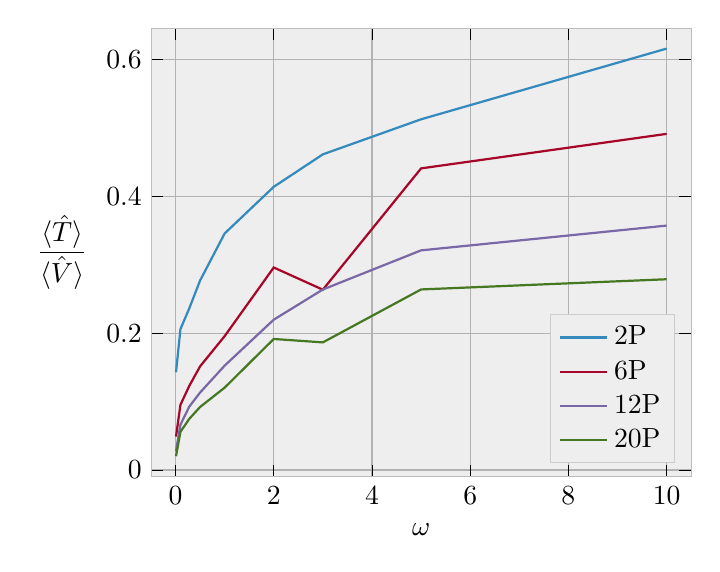
\begin{tikzpicture}

\definecolor{color0}{rgb}{0.203921568627451,0.541176470588235,0.741176470588235}
\definecolor{color1}{rgb}{0.650980392156863,0.0235294117647059,0.156862745098039}
\definecolor{color2}{rgb}{0.47843137254902,0.407843137254902,0.650980392156863}
\definecolor{color3}{rgb}{0.274509803921569,0.470588235294118,0.129411764705882}

\begin{axis}[
axis background/.style={fill=white!93.33333333333333!black},
axis line style={white!73.72549019607844!black},
legend cell align={left},
legend style={at={(0.97,0.03)}, anchor=south east, draw=white!80.0!black, fill=white!93.33333333333333!black},
tick pos=both,
x grid style={white!69.80392156862744!black},
xlabel={\(\displaystyle \omega\)},
xmajorgrids,
xmin=-0.4895, xmax=10.4995,
xtick style={color=black},
y grid style={white!69.80392156862744!black},
ylabel style={rotate=-90.0},
ylabel={\(\displaystyle \frac{\langle\hat{T}\rangle}{\langle\hat{V}\rangle}\)},
ymajorgrids,
ymin=-0.00950153433365221, ymax=0.645814840406007,
ytick style={color=black}
]
\addplot [thick, color0]
table {%
0.01 0.14292980671414
0.1 0.206000508517671
0.28 0.236346842166032
0.5 0.277065579844387
1 0.345784185233727
2 0.41399969664796
3 0.461449773987519
5 0.512681528738802
10 0.616027732463295
};
\addlegendentry{2P}
\addplot [thick, color1]
table {%
0.01 0.0489614243323442
0.1 0.0953652097389264
0.28 0.123020257826888
0.5 0.151552210724365
1 0.195728715728716
2 0.296060131091479
3 0.263623577547628
5 0.440925380415408
10 0.491388484677367
};
\addlegendentry{6P}
\addplot [thick, color2]
table {%
0.01 0.0279279279279279
0.1 0.0663141106354403
0.28 0.0927190456602221
0.5 0.113307273027584
1 0.152620094780267
2 0.21978952717725
3 0.263891885843983
5 0.321107495449782
10 0.357318784099766
};
\addlegendentry{12P}
\addplot [thick, color3]
table {%
0.01 0.0202855736090596
0.1 0.0558188176084186
0.28 0.0748673013733255
0.5 0.092181964299863
1 0.120447174205168
2 0.191577362501107
3 0.186589637000426
5 0.263982205508037
10 0.278872126802915
};
\addlegendentry{20P}
\end{axis}

\end{tikzpicture}}}
	\subfloat[RBM+SJ]{{% This file was created by tikzplotlib v0.8.1.
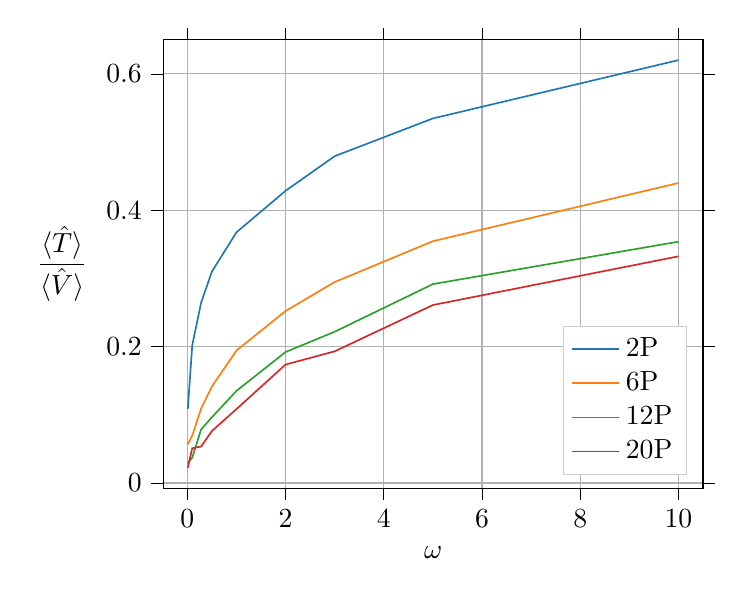
\begin{tikzpicture}

\definecolor{color0}{rgb}{0.12156862745098,0.466666666666667,0.705882352941177}
\definecolor{color1}{rgb}{1,0.498039215686275,0.0549019607843137}
\definecolor{color2}{rgb}{0.172549019607843,0.627450980392157,0.172549019607843}
\definecolor{color3}{rgb}{0.83921568627451,0.152941176470588,0.156862745098039}

\begin{axis}[
legend cell align={left},
legend style={at={(0.97,0.03)}, anchor=south east, draw=white!80.0!black},
tick align=outside,
tick pos=both,
x grid style={white!69.01960784313725!black},
xlabel={\(\displaystyle \omega\)},
xmajorgrids,
xmin=-0.4895, xmax=10.4995,
xtick style={color=black},
y grid style={white!69.01960784313725!black},
ylabel style={rotate=-90.0},
ylabel={\(\displaystyle \frac{\langle\hat{T}\rangle}{\langle\hat{V}\rangle}\)},
ymajorgrids,
ymin=-0.00739548914049018, ymax=0.649881709767761,
ytick style={color=black}
]
\addplot [semithick, color0]
table {%
0.01 0.108705258506407
0.1 0.202009646302251
0.28 0.264296187683284
0.5 0.310018755861207
1 0.367553865652725
2 0.428427393293865
3 0.479188481675393
5 0.534512711346008
10 0.620005473453749
};
\addlegendentry{2P}
\addplot [semithick, color1]
table {%
0.01 0.0567119155354449
0.1 0.0697142186491403
0.28 0.109019214224262
0.5 0.141514485132422
1 0.194234043802478
2 0.252176075603084
3 0.294666494223597
5 0.354539716887567
10 0.439893538370546
};
\addlegendentry{6P}
\addplot [semithick, color2]
table {%
0.01 0.0288659793814433
0.1 0.0372200263504611
0.28 0.0784915858002702
0.5 0.096412072256494
1 0.135095692138839
2 0.192092791484218
3 0.221784714644907
5 0.291641379310345
10 0.353855680855225
};
\addlegendentry{12P}
\addplot [semithick, color3]
table {%
0.01 0.0224807471735212
0.1 0.0510365183964855
0.28 0.0535270823545204
0.5 0.0761996706229769
1 0.108428284656055
2 0.17366909653192
3 0.19307880632568
5 0.260942252768941
10 0.332349732889548
};
\addlegendentry{20P}
\end{axis}

\end{tikzpicture}}}\\
	\subfloat[RBM+PJ]{{% This file was created by tikzplotlib v0.8.1.
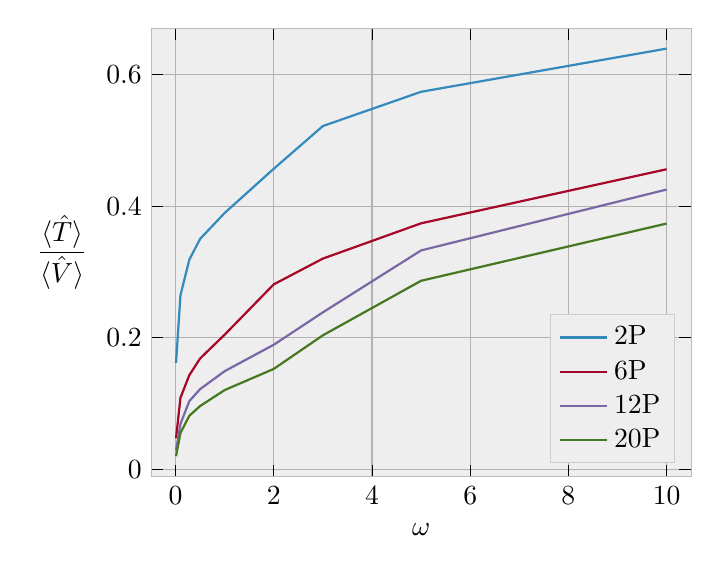
\begin{tikzpicture}

\definecolor{color0}{rgb}{0.203921568627451,0.541176470588235,0.741176470588235}
\definecolor{color1}{rgb}{0.650980392156863,0.0235294117647059,0.156862745098039}
\definecolor{color2}{rgb}{0.47843137254902,0.407843137254902,0.650980392156863}
\definecolor{color3}{rgb}{0.274509803921569,0.470588235294118,0.129411764705882}

\begin{axis}[
axis background/.style={fill=white!93.33333333333333!black},
axis line style={white!73.72549019607844!black},
legend cell align={left},
legend style={at={(0.97,0.03)}, anchor=south east, draw=white!80.0!black, fill=white!93.33333333333333!black},
tick pos=both,
x grid style={white!69.80392156862744!black},
xlabel={\(\displaystyle \omega\)},
xmajorgrids,
xmin=-0.4895, xmax=10.4995,
xtick style={color=black},
y grid style={white!69.80392156862744!black},
ylabel style={rotate=-90.0},
ylabel={\(\displaystyle \frac{\langle\hat{T}\rangle}{\langle\hat{V}\rangle}\)},
ymajorgrids,
ymin=-0.011155128448522, ymax=0.670716886119897,
ytick style={color=black}
]
\addplot [thick, color0]
table {%
0.01 0.161598746081505
0.1 0.264466364626943
0.28 0.318533815178111
0.5 0.350256285086649
1 0.389730328777244
2 0.456965583072599
3 0.52190696776684
5 0.574018126888218
10 0.639722703639515
};
\addlegendentry{2P}
\addplot [thick, color1]
table {%
0.01 0.0468986384266263
0.1 0.108489101409675
0.28 0.142927927927928
0.5 0.168400011874487
1 0.204595643091614
2 0.281150742944763
3 0.320306803143652
5 0.373984932084395
10 0.456212770963223
};
\addlegendentry{6P}
\addplot [thick, color2]
table {%
0.01 0.0287417763157895
0.1 0.0689267491135519
0.28 0.103510351035104
0.5 0.121754035137837
1 0.149081447331657
2 0.189290836653386
3 0.238556500646571
5 0.332749562171629
10 0.425379527774922
};
\addlegendentry{12P}
\addplot [thick, color3]
table {%
0.01 0.0198390540318607
0.1 0.0550696242390316
0.28 0.0812272164373049
0.5 0.0960548685344326
1 0.120346512979882
2 0.152555093728466
3 0.20363356015151
5 0.286590458917023
10 0.373618884667807
};
\addlegendentry{20P}
\end{axis}

\end{tikzpicture}}}
	\subfloat[VMC]{{% This file was created by tikzplotlib v0.8.1.
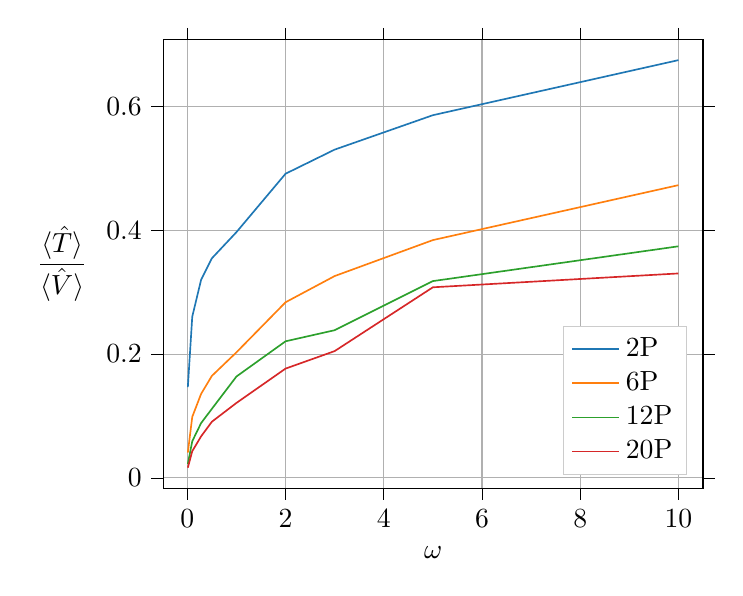
\begin{tikzpicture}

\definecolor{color0}{rgb}{0.12156862745098,0.466666666666667,0.705882352941177}
\definecolor{color1}{rgb}{1,0.498039215686275,0.0549019607843137}
\definecolor{color2}{rgb}{0.172549019607843,0.627450980392157,0.172549019607843}
\definecolor{color3}{rgb}{0.83921568627451,0.152941176470588,0.156862745098039}

\begin{axis}[
legend cell align={left},
legend style={at={(0.97,0.03)}, anchor=south east, draw=white!80.0!black},
tick align=outside,
tick pos=both,
x grid style={white!69.01960784313725!black},
xlabel={\(\displaystyle \omega\)},
xmajorgrids,
xmin=-0.4895, xmax=10.4995,
xtick style={color=black},
y grid style={white!69.01960784313725!black},
ylabel style={rotate=-90.0},
ylabel={\(\displaystyle \frac{\langle\hat{T}\rangle}{\langle\hat{V}\rangle}\)},
ymajorgrids,
ymin=-0.0164668337421715, ymax=0.707728537231861,
ytick style={color=black}
]
\addplot [semithick, color0]
table {%
0.01 0.146594427244582
0.1 0.260418749464423
0.28 0.319901846829394
0.5 0.354717597127
1 0.396972519795063
2 0.491318502441671
3 0.53027950310559
5 0.585870116692034
10 0.67481056582395
};
\addlegendentry{2P}
\addplot [semithick, color1]
table {%
0.01 0.0407722122838402
0.1 0.0985104942450914
0.28 0.135666711367395
0.5 0.164801025691602
1 0.202835527491511
2 0.28369079862382
3 0.326016767506851
5 0.384115256741781
10 0.472868887927304
};
\addlegendentry{6P}
\addplot [semithick, color2]
table {%
0.01 0.0225470925470925
0.1 0.0591952540624194
0.28 0.0885030700825746
0.5 0.111576919808515
1 0.163770657314416
2 0.220633968028807
3 0.238556500646571
5 0.317885405699147
10 0.37406475534662
};
\addlegendentry{12P}
\addplot [semithick, color3]
table {%
0.01 0.0164511376657391
0.1 0.0430938843433643
0.28 0.067074638154502
0.5 0.0907330085826954
1 0.121087634122869
2 0.176534004132603
3 0.20481414099371
5 0.307872099467483
10 0.330233868695407
};
\addlegendentry{20P}
\end{axis}

\end{tikzpicture}}}
	\caption{The kinetic-potential energy ratio $\langle\hat{T}\rangle/\langle\hat{V}\rangle$ plotted as a function of the oscillator frequency for two-dimensional circular quantum dots. The frequencies $\omega=0.01, 0.1, 0.28, 0.5, 1.0, 2.0, 3.0, 5.0, 10.0$ were run. For abbreviations see the text.}
	\label{fig:energysplitVMC2D}
\end{figure}
\fi

\subsection{Energy distribution} \label{sec:energydistributions}
If we now recall the general Hamiltonian presented in chapter \ref{chp:manybody}, the total energy is just the sum of the kinetic energy, harmonic oscillator potential energy and interaction energy. As the variational Monte Carlo method attempts to solve the Schrödinger equation directly, it is trivial to find the distribution between the various energy sources. Finding this is in general interesting when we want to exploit the most important contributions to the energy. Additionally, we can use these results to check the virial theorem presented in section \ref{sec:virial}. It is also interesting to see if the different ansätze give different energy distributions. We will denote the kinetic energy by $\langle\hat{T}\rangle$. The harmonic oscillator potential energy is associated with the more general term external potential energy, and is denoted by $\langle\hat{V}_{\text{ext}}\rangle$. The electron-electron interaction potential energy, or just the interaction energy, is denoted by $\langle\hat{V}_{\text{int}}\rangle$. In figure \eqref{fig:energydistribution}, we plot the ratio between the kinetic energy and total potential energy ($\langle\hat{V}\rangle=\langle\hat{V}_{\text{ext}}\rangle+\langle\hat{V}_{\text{int}}\rangle$) as a function of the oscillator frequency. The systems considered are two-dimensional quantum dots with up to $N=20$ electrons. We base the plots on the numbers in the tables (\ref{tab:splitfrequencyQDRBM}-\ref{tab:splitfrequencyQDVMC}) in appendix \ref{chp:totalresults}.

% This file was created by tikzplotlib v0.8.1.
\begin{figure}
\begin{tikzpicture}

\begin{axis}[
legend cell align={left},
legend style={at={(1.7,1.15)}, anchor=south east, draw=white!80.0!black},
legend columns = 4,
title={RBM},
title style={yshift=-1.5ex},
%tick align=outside,
tick pos=both,
x grid style={white!69.01960784313725!black},
%xlabel={\(\displaystyle \omega\)},
width=8cm,
height=5cm,
xmajorgrids,
xmin=-0.4895, xmax=10.4995,
xtick style={color=black},
y grid style={white!69.01960784313725!black},
ylabel style={rotate=-90.0},
ylabel={\(\displaystyle \frac{\langle\hat{T}\rangle}{\langle\hat{V}\rangle}\)},
ymajorgrids,
ymin=-0.03, ymax=0.7,
ytick style={color=black}
]
\addplot [thick, color0]
table {%
	0.01 0.14292980671414
	0.1 0.206000508517671
	0.28 0.236346842166032
	0.5 0.277065579844387
	1 0.345784185233727
	2 0.41399969664796
	3 0.461449773987519
	5 0.512681528738802
	10 0.616027732463295
};
\addlegendentry{$N=2$}
\addplot [thick, color1]
table {%
	0.01 0.0489614243323442
	0.1 0.0953652097389264
	0.28 0.123020257826888
	0.5 0.151552210724365
	1 0.195728715728716
	2 0.296060131091479
	3 0.363623577547628
	5 0.440925380415408
	10 0.491388484677367
};
\addlegendentry{$N=6$}
\addplot [thick, color2]
table {%
	0.01 0.0279279279279279
	0.1 0.0663141106354403
	0.28 0.0927190456602221
	0.5 0.113307273027584
	1 0.152620094780267
	2 0.21978952717725
	3 0.263891885843983
	5 0.321107495449782
	10 0.357318784099766
};
\addlegendentry{$N=12$}
\addplot [thick, color3]
table {%
	0.01 0.0202855736090596
	0.1 0.0558188176084186
	0.28 0.0748673013733255
	0.5 0.092181964299863
	1 0.120447174205168
	2 0.191577362501107
	3 0.2257693437
	5 0.263982205508037
	10 0.278872126802915
};
\addlegendentry{$N=20$}
\end{axis}

\begin{axis}[
xshift=7.7cm,
legend cell align={left},
legend style={at={(0.97,0.03)}, anchor=south east, draw=white!80.0!black},
%tick align=outside,
title={RBM+SJ},
title style={yshift=-1.5ex},
tick pos=both,
x grid style={white!69.01960784313725!black},
%xlabel={\(\displaystyle \omega\)},
xmajorgrids,
width=8cm,
height=5cm,
xmin=-0.4895, xmax=10.4995,
xtick style={color=black},
y grid style={white!69.01960784313725!black},
%ylabel style={rotate=-90.0},
%ylabel={\(\displaystyle \frac{\langle\hat{T}\rangle}{\langle\hat{V}\rangle}\)},
ymajorgrids,
ymin=-0.03, ymax=0.7,
ytick style={color=black}
]
\addplot [thick, color0]
table {%
	0.01 0.108705258506407
	0.1 0.202009646302251
	0.28 0.264296187683284
	0.5 0.310018755861207
	1 0.367553865652725
	2 0.428427393293865
	3 0.479188481675393
	5 0.534512711346008
	10 0.620005473453749
};
%\addlegendentry{2P}
\addplot [thick, color1]
table {%
	0.01 0.0567119155354449
	0.1 0.0697142186491403
	0.28 0.109019214224262
	0.5 0.141514485132422
	1 0.194234043802478
	2 0.252176075603084
	3 0.294666494223597
	5 0.354539716887567
	10 0.439893538370546
};
%\addlegendentry{6P}
\addplot [thick, color2]
table {%
	0.01 0.0288659793814433
	0.1 0.0372200263504611
	0.28 0.0784915858002702
	0.5 0.096412072256494
	1 0.135095692138839
	2 0.192092791484218
	3 0.221784714644907
	5 0.291641379310345
	10 0.353855680855225
};
%\addlegendentry{12P}
\addplot [thick, color3]
table {%
	0.01 0.0224807471735212
	0.1 0.0510365183964855
	0.28 0.0535270823545204
	0.5 0.0761996706229769
	1 0.108428284656055
	2 0.17366909653192
	3 0.19307880632568
	5 0.260942252768941
	10 0.332349732889548
};
%\addlegendentry{20P}
\end{axis}

\end{tikzpicture}

\begin{tikzpicture}

\begin{axis}[
legend cell align={left},
legend style={at={(0.97,1.03)}, anchor=south east, draw=white!80.0!black},
%tick align=outside,
title={RBM+PJ},
title style={yshift=-1.5ex},
tick pos=both,
x grid style={white!69.01960784313725!black},
xlabel={\(\displaystyle \omega\)},
width=8cm,
height=5cm,
xmajorgrids,
xmin=-0.4895, xmax=10.4995,
xtick style={color=black},
y grid style={white!69.01960784313725!black},
ylabel style={rotate=-90.0},
ylabel={\(\displaystyle \frac{\langle\hat{T}\rangle}{\langle\hat{V}\rangle}\)},
ymajorgrids,
ymin=-0.03, ymax=0.75,
ytick style={color=black}
]
\addplot [thick, color0]
table {%
	0.01 0.161598746081505
	0.1 0.264466364626943
	0.28 0.318533815178111
	0.5 0.350256285086649
	1 0.389730328777244
	2 0.456965583072599
	3 0.52190696776684
	5 0.574018126888218
	10 0.639722703639515
};
%\addlegendentry{2P}
\addplot [thick, color1]
table {%
	0.01 0.0468986384266263
	0.1 0.108489101409675
	0.28 0.142927927927928
	0.5 0.168400011874487
	1 0.204595643091614
	2 0.281150742944763
	3 0.320306803143652
	5 0.373984932084395
	10 0.456212770963223
};
%\addlegendentry{6P}
\addplot [thick, color2]
table {%
	0.01 0.0287417763157895
	0.1 0.0689267491135519
	0.28 0.103510351035104
	0.5 0.121754035137837
	1 0.149081447331657
	2 0.189290836653386
	3 0.238556500646571
	5 0.332749562171629
	10 0.425379527774922
};
%\addlegendentry{12P}
\addplot [thick, color3]
table {%
	0.01 0.0198390540318607
	0.1 0.0550696242390316
	0.28 0.0812272164373049
	0.5 0.0960548685344326
	1 0.120346512979882
	2 0.152555093728466
	3 0.20363356015151
	5 0.286590458917023
	10 0.373618884667807
};
%\addlegendentry{20P}
\node[] at (axis cs: 5,-.25) {RBM+PJ};
\end{axis}

\begin{axis}[
xshift=7.7cm,
legend cell align={left},
legend style={at={(0.97,0.03)}, anchor=south east, draw=white!80.0!black},
%tick align=outside,
title={VMC},
title style={yshift=-1.5ex},
tick pos=both,
x grid style={white!69.01960784313725!black},
xlabel={\(\displaystyle \omega\)},
xmajorgrids,
width=8cm,
height=5cm,
xmin=-0.4895, xmax=10.4995,
xtick style={color=black},
y grid style={white!69.01960784313725!black},
%ylabel style={rotate=-90.0},
%ylabel={\(\displaystyle \frac{\langle\hat{T}\rangle}{\langle\hat{V}\rangle}\)},
ymajorgrids,
ymin=-0.03, ymax=0.75,
ytick style={color=black}
]
\addplot [thick, color0]
table {%
	0.01 0.146594427244582
	0.1 0.260418749464423
	0.28 0.319901846829394
	0.5 0.354717597127
	1 0.396972519795063
	2 0.491318502441671
	3 0.53027950310559
	5 0.585870116692034
	10 0.67481056582395
};

\addplot [thick, color1]
table {%
	0.01 0.0407722122838402
	0.1 0.0985104942450914
	0.28 0.135666711367395
	0.5 0.164801025691602
	1 0.202835527491511
	2 0.28369079862382
	3 0.326016767506851
	5 0.384115256741781
	10 0.472868887927304
};

\addplot [thick, color2]
table {%
	0.01 0.0225470925470925
	0.1 0.0591952540624194
	0.28 0.0885030700825746
	0.5 0.111576919808515
	1 0.163770657314416
	2 0.220633968028807
	3 0.238556500646571
	5 0.317885405699147
	10 0.37406475534662
};

\addplot [thick, color3]
table {%
	0.01 0.0164511376657391
	0.1 0.0430938843433643
	0.28 0.067074638154502
	0.5 0.0907330085826954
	1 0.121087634122869
	2 0.176534004132603
	3 0.20481414099371
	5 0.307872099467483
	10 0.330233868695407
};
\end{axis}

\end{tikzpicture}
\caption{The kinetic-potential energy ratio, $\langle\hat{T}\rangle/\langle\hat{V}\rangle$, plotted as a function of the oscillator frequency for two-dimensional quantum dots with $N=2$, 6, 12 and 20 electrons. Simulations with frequencies $\omega=0.01,$ 0.1, 0.28, 0.5, 1.0, 2.0, 3.0, 5.0, 10.0 were performed, see appendix \ref{chp:totalresults} for exact energies. For  abbreviations and description of the natural units used, see the text.}
\label{fig:energydistribution}
\end{figure}

Firstly, the graphs are very similar for all the ansätze, which means that they all give the same distribution between kinetic energy and total potential energy, although they do not provide the same total energy. This is an interesting observation and indicates that both the obtained kinetic energy, total potential energy differ for the various ansätze when the total energy is different. Physically, this means that the electron configurations are fundamentally different for the different ansätze, as the electron configuration is the only factor that alters the potential energy. This was already observed in the one-body density plots. Further, we see a significant trend where the ratio drops as the frequency is decreased, implying that the total potential energy dominates over the kinetic energy at low frequencies. This is a known phenomenon already mentioned several times throughout this thesis. The ratio is consequently lower for larger dots. This is a result of gradually more interaction energy as we increase the number of electrons. 

\begin{table}
	\caption{The ground state energy, $E$, of two-dimensional quantum dots with $N=12$ electrons and frequency $\omega$. In the following columns, the distribution between kinetic, $\langle\hat{T}\rangle$, external potential, $\langle\hat{V}_{\text{ext}}\rangle$, and interaction, $\langle\hat{V}_{\text{int}}\rangle$, energy are presented. The energy is given in units of $\hbar$ (natural units), and the numbers in parenthesis are the statistical uncertainties in the last digit. For abbreviations see the text.}
	\label{tab:splitfrequencyQD20P}
	\begin{tabularx}{\textwidth}{R{0.5cm}rrcR{2.3cm}R{2.3cm}R{2.3cm}R{2.3cm}R{0.3cm}} \hline\hline
		&\makecell{\\ \phantom{$N$}} & $\omega$ && \multicolumn{1}{c}{$E$} & \multicolumn{1}{c}{$\langle \hat{T}\rangle$} & \multicolumn{1}{c}{$\langle \hat{V}_{\text{ext}} \rangle$} & \multicolumn{1}{c}{$\langle \hat{V}_{\text{int}} \rangle$} \\ \hline \\
		&RBM & 0.01 && 6.217(2) & 0.1236(4) & 2.244(2) & 3.849(2) \\
		&& 2.0 && 269.086(8) & 43.262(8) & 95.17(2) & 130.65(1) \\
		&& 10.0 && 961.03(4) & 260.2(1) & 364.8(1) & 336.06(7) \\
		\hline \\
		
		&RBM+SJ & 0.01 && 6.239(2) & 0.1372(6) & 2.184(2) & 3.919(3) \\
		&& 2.0 && 265.66(9) & 39.31(8) & 95.78(1) & 130.57(2) \\
		&& 10.0 && 952.71(2) & 237.65(4) & 392.06(7) & 323.00(3) \\
		\hline \\
		
		&RBM+PJ & 0.01 && 6.210(1) & 0.1208(5) & 2.189(2) & 3.900(2) \\
		&& 2.0 && 262.598(1) & 34.758(6) & 108.546(9) & 119.293(7) \\
		&& 10.0 && 947.33(2) & 257.67(5) & 348.35(6) & 341.31(3) \\ 
		\hline \\
		
		&VMC & 0.01 && 6.2097(8) & 0.1005(4) & 2.270(3) & 3.839(3) \\
		&& 2.0 && 262.5339(9) & 38.402(3) & 95.681(7) & 128.451(5) \\
		&& 10.0 && 945.596(8) & 231.56(4) & 389.26(7) & 324.77(3) \\
		\hline\hline
	\end{tabularx}
\end{table}

If we further recall the virial theorem presented in section \ref{sec:virial}, it states that the kinetic energy is related to the potential energies in a certain way. We have tested the virial theorem for non-interacting quantum dots and verified a modified virial theorem, $\langle\hat{T}\rangle=\langle\hat{V}_{\text{ext}}\rangle$, deduced from equation \eqref{eq:simplevirial}. When we do the same calculation for the correlated quantum dots, we find the relation to not be satisfied. This can be seen from table \eqref{tab:splitfrequencyQD20P}, where we present the energy distribution for two-dimensional quantum dots with $N=12$ and selected frequencies. Especially for low frequency dots, the kinetic energy is much smaller than the interaction energy. When the frequency is increased, the interacting energy contributes less. The kinetic and total potential energy then approach the same energy. This can also be seen from figure \eqref{fig:energydistribution}, as the graphs flatten out as the frequency increases. Based on this, we believe that $\langle\hat{T}\rangle\simeq\langle\hat{V}_{\text{ext}}\rangle$ when $\omega\rightarrow\infty$. This finding highlights that the behavior of the interacting system approaches the non-interacting behavior as the frequency increases, indicating that the one-body contributions dominate. The interaction contribution is apparently less important for high-frequency dots. This is paradoxical as the average electron-electron distance is small when the frequency is high. Contrarily, the interactions are more important for low-frequency dots. The range of the Coulomb interactions is infinite, making the electrons affect each other even at long distances. To reduce the range of the Coulomb potential, we can introduce a screened Coulomb potential. With $r_{ij}$ as the distance between two electrons $i$ and $j$, the effective interaction potential using screened potential may take the form
\begin{equation}
\hat{V}_{\text{int}}=\sum_{i=1}^N\sum_{j>i}^N\frac{\exp(-r_{ij}/\mu)}{r_{ij}}
\end{equation}
where $\mu$ is a screening parameter. Depending on the values of $\mu$, the screened potential can drop quickly to zero. This can, for instance, be representative for quantum dots in dielectric media. We have simulated low-frequency quantum dots using the Coulomb screening potential, and observed that the kinetic energy and the external potential energy are almost identical for appropriate values of $\mu$. We expected this to happen as the electron-electron distances are relatively large when the frequency is low, resulting in a minimum of interaction energy using the screened potential. \iffalse The findings are directly in line with observations in previous research.\fi

Another interesting aspect is how the energy is distributed for the various ansätze. Most notably, we see that VMC and RBM+PJ provide different kinetic and total potential energy distributions, albeit the total energy is more or less identical. Physically, this means that RBM+PJ finds another electron configuration than VMC to minimize the energy, which is exciting as the former ansatz is supposed to be more flexible than the latter. For more frequencies and system sizes, see appendix \ref{chp:totalresults}.

\begin{figure}
	\centering
	\captionsetup[subfigure]{labelformat=empty}
	\subfloat{\raisebox{1.5cm}{\rotatebox[origin=t]{90}{RBM}}}\hspace{0.1cm}
	\subfloat{{\includegraphics[width=5.1cm]{../plots/int1/onebody2/2D/2P/0.100000w/RBM_ADAM_MC1048576.png}}}\hspace{-0.cm}
	\subfloat{{\includegraphics[width=5.1cm]{../plots/int1/onebody2/2D/6P/0.100000w/RBM_ADAM_MC1048576.png}}}\hspace{-0.cm}
	\subfloat{{\includegraphics[width=5.1cm]{../plots/int1/onebody2/2D/12P/0.100000w/RBM_ADAM_MC1048576.png}}}\\ [-0.cm]
	
	\subfloat{\raisebox{1.5cm}{\rotatebox[origin=t]{90}{VMC}}}\hspace{0.1cm}
	\subfloat[$N=2$]{{\includegraphics[width=5.1cm]{../plots/int1/onebody2/2D/2P/0.100000w/VMC_ADAM_MC1048576.png}}}\hspace{-0.cm}
	\subfloat[$N=6$]{{\includegraphics[width=5.1cm]{../plots/int1/onebody2/2D/6P/0.100000w/VMC_ADAM_MC1048576.png}}}\hspace{-0.cm}
	\subfloat[$N=12$]{{\includegraphics[width=5.1cm]{../plots/int1/onebody2/2D/12P/0.100000w/VMC_ADAM_MC1048576.png}}}
	
	\caption{Plots of the one-body density profile, $\rho(x, y)$, of two-dimensional quantum dots with frequency $\omega=0.1$ and $N=2$, 6 and 12 electrons seen from left to right. The ansätze used are RBM (upper plots) and VMC (lower plots). The surface plot and the contour plot on the $xy$-plane illustrate the density, and the graph on the $yz$-plane represents the cross-section through $x=0$. The surface plots are noise-reduced using a Savitzky-Golay filter. For abbreviations and description of the natural units used, see the text.}
	\label{fig:lowfreqRBM}
\end{figure}

\newpage
\subsection{Low frequency dots} \label{sec:lowfrequencies}
In section \ref{sec:onebodyresults}, we found the one-body density to be shape-invariant for high-frequency dots with $\omega\geq0.28$. However, when we further decreased the frequency down to $\omega=0.1$, the density profiles changed significantly, and we got other extrema. This section aims to investigate the transitions between the various shapes with frequencies down to $\omega=0.01$. At this points, it is important to recall that our choice of the trial wave function is a single Slater determinant. This is not necessarily a good approximation for these low-frequency dots, as the energy gaps between the excited states around the Fermi level are small. 

We start by looking at quantum dots with frequency $\omega=0.1$, and in figure \eqref{fig:lowfreqRBM} we compare the spatial density profiles for $N=2$, 6 and 12 produced using RBM and VMC. The density profiles appear to be completely different. While VMC provides a single peak with some bumps on the top, RBM gives more distinct peaks. The numbers of peaks for the RBM ansatz is equal to the number of electrons, which indicates that the RBM finds the electrons to be localized at some fixed spots. The two ansätze model the correlations in completely different ways, and as the correlations become more important for low frequencies, it was expected that the results would also be different. However, the ground state energies obtained by the two ansätze do not differ this much for the same systems. This indicates that the electron density plots are better to reveal differences between the ansätze than the energy itself. 

\begin{figure}
	\centering
	\captionsetup[subfigure]{labelformat=empty}
	\subfloat{\raisebox{1.5cm}{\rotatebox[origin=t]{90}{RBM+PJ}}}\hspace{0.1cm}
	\subfloat{{\includegraphics[width=5.1cm]{../plots/int1/onebody2/2D/2P/0.280000w/RBMPJ_ADAM_MC1048576.png}}}\hspace{-0.cm}
	\subfloat{{\includegraphics[width=5.1cm]{../plots/int1/onebody2/2D/2P/0.100000w/RBMPJ_ADAM_MC1048576.png}}}\hspace{-0.cm}
	\subfloat{{\includegraphics[width=5.1cm]{../plots/int1/onebody2/2D/2P/0.010000w/RBMPJ_ADAM_MC2pow28_smooth_blue_small.png}}}\\ [-0.cm]
	
	\subfloat{\raisebox{1.5cm}{\rotatebox[origin=t]{90}{VMC}}}\hspace{0.1cm}
	\subfloat[$\omega=0.28$]{{\includegraphics[width=5.1cm]{../plots/int1/onebody2/2D/2P/0.280000w/VMC_ADAM_MC1048576.png}}}\hspace{-0.cm}
	\subfloat[$\omega=0.1$]{{\includegraphics[width=5.1cm]{../plots/int1/onebody2/2D/2P/0.100000w/VMC_ADAM_MC1048576.png}}}\hspace{-0.cm}
	\subfloat[$\omega=0.01$]{{\includegraphics[width=5.1cm]{../plots/int1/onebody2/2D/2P/0.010000w/VMC_ADAM_MC2pow28_smooth_blue_small.png}}}
	
	\caption{Plots of the one-body density profile, $\rho(x, y)$, of two-dimensional quantum dots with $N=2$ electrons and frequencies $\omega=0.28$, 0.1 and 0.01 from left to right. The ansätze used are RBM+PJ (upper plots) and VMC (lower plots). The surface plot and the contour plot on the $xy$-plane illustrate the density, and the graph on the $yz$-plane represents the cross-section through $x=0$. The surface plots are noise-reduced using a Savitzky-Golay filter. For  abbreviations and description of the natural units used, see the text.}
	\label{fig:lowfreq2P}
\end{figure}

Furthermore, in figure \eqref{fig:lowfreq2P} we fix the number of electrons to be $N=2$, and vary the frequency from $\omega=0.28$ down to $\omega=0.01$ with density profiles produced by VMC and RBM+PJ. These ansätze were selected as they hitherto have provided the lowest ground state energies and we want to see if RBM+PJ can reveal effects that VMC is not able to capture. We see that the two ansätze obtain very similar density plots, where they agree that a ridge around the center of the dot should be more distinct as the frequency drops. If we go back to figure \eqref{fig:energydistribution}, we saw that the kinetic energy was negligible for the lowest energies, and the effect is therefore an indication of the Wigner localization effect discussed in section \ref{sec:wigner}. As in the classical limit, the two electrons will repel each other and seldom be located at the same place when their kinetic energy is low. RBM+PJ possibly provides a sharper ridge for $\omega=0.01$, which is closer to the DMC results found in \citet{hogberget_quantum_2013} and thus perhaps more correct. However, the energy provided by RBM+PJ and VMC are more or less identical ($E=0.074107$ and $E=0.074070$, respectively), which means that the difference in one-body density does not affect energy.

\begin{figure}
	\centering
	\captionsetup[subfigure]{labelformat=empty}
	\subfloat{\raisebox{1.5cm}{\rotatebox[origin=t]{90}{RBM+PJ}}}\hspace{0.1cm}
	\subfloat{{\includegraphics[width=5.1cm]{../plots/int1/onebody2/2D/6P/0.280000w/RBMPJ_ADAM_MC1048576.png}}}\hspace{-0.cm}
	\subfloat{{\includegraphics[width=5.1cm]{../plots/int1/onebody2/2D/6P/0.100000w/RBMPJ_ADAM_MC1048576.png}}}\hspace{-0.cm}
	\subfloat{{\includegraphics[width=5.1cm]{../plots/int1/onebody2/2D/6P/0.010000w/RBMPJ_ADAM_MC1048576.png}}}\\ [-0.cm]
	
	\subfloat{\raisebox{1.5cm}{\rotatebox[origin=t]{90}{VMC}}}\hspace{0.1cm}
	\subfloat[$\omega=0.28$]{{\includegraphics[width=5.1cm]{../plots/int1/onebody2/2D/6P/0.280000w/VMC_ADAM_MC1048576.png}}}\hspace{-0.cm}
	\subfloat[$\omega=0.1$]{{\includegraphics[width=5.1cm]{../plots/int1/onebody2/2D/6P/0.100000w/VMC_ADAM_MC1048576.png}}}\hspace{-0.cm}
	\subfloat[$\omega=0.01$]{{\includegraphics[width=5.1cm]{../plots/int1/onebody2/2D/6P/0.010000w/VMC_ADAM_MC2pow28_smooth}}}
	
	\caption{Plots of the one-body density profile, $\rho(x, y)$, of two-dimensional quantum dots with $N=6$ electrons and frequencies $\omega=0.28$, 0.1 and 0.01 seen from left to right. The ansätze used are RBM+PJ (upper plots) and VMC (lower plots). The surface plot and the contour plot on the $xy$-plane illustrate the density, and the graph on the $yz$-plane represents the cross-section through $x=0$. The surface plots are noise-reduced using a Savitzky-Golay filter. For  abbreviations and description of the natural units used, see the text.}
	\label{fig:lowfreq6P}
\end{figure}

% Contrary to the findings of __ we did not find __
We repeat the exercise for quantum dots with $N=6$ electrons, and obtain the plots in figure \eqref{fig:lowfreq6P}. With VMC, we observe the same tendency as for the dots with $N=2$ electrons, where we get an additional peak in the density plot as the frequency decreases. However, for RBM+PJ we do not get this peak in the center, but rather a significant density drop. This is contrary to the DMC one-body density plots obtained by \citet{hogberget_quantum_2013}, where there is a sharp peak in the center. The density plot for quantum dots is also to approach the classical limit as the frequency is decreased \supercite{ghosal_incipient_2007}, where the potential energy is minimized when we have one electron in the center and five electrons surrounding it.

In order to give a more qualitative comparison of the various ansätze, we also present the radial one-body density profiles. In figure \eqref{fig:lowfreq}, the one-body density of quantum dots with frequency $\omega=0.01$ and $N=2$, 6 electrons is presented. We see that the ansätze agree on the density shape for $N=2$, where RBM+PJ gives the most distinct peak, followed by VMC, RBM+SJ and RBM, in that order. For $N=6$, the various ansätze give completely different density profiles. The variation might again be explained by different approaches to model the correlations, but future investigations on this is needed.

\begin{figure}
	\centering
	\captionsetup[subfigure]{labelformat=empty}
	\subfloat{{\includegraphics[width=\textwidth/2]{../plots/int1/onebody/2D/2P/0.010000w/ADAM_MC1048576.eps}}}
  	\subfloat{{\includegraphics[width=\textwidth/2]{../plots/int1/onebody/2D/6P/0.010000w/ADAM_MC10485762.eps}}}
	
	\caption{Plots of the one-body density profile, $\rho(r)$, of two-dimensional quantum dots of frequency $\omega=0.01$ and $N=72$, 90. The ADAM optimizer was used, and after convergence the number of Monte Carlo cycles was $M=2^{28}=268,435,456$. For abbreviations and description of the natural units used, see the text.}
	\label{fig:lowfreq}
\end{figure}

\subsection{Large dots}
In order to test the code, we also decided to run for systems with $N>56$. We do this for the sake of completeness and to test how far a VMC code can go. One thing is that the computations get extremely expensive as the number of electrons increases, but we have also seen that the statistical error increases as the system size increases. This means that we cannot just crack up the wall clock time and wait when studying large systems; at some point, the standard error gets too large and we need to increase the number of Monte Carlo cycles further. The learning rate also needs to be decreased as the system size increases, which requires more iterations. In table \eqref{tab:largeQD}, the ground state energy of two-dimensional quantum dots with frequency $\omega=1.0$, and $N=72$, 90 electrons and three-dimensional quantum dots with $N=70$ electrons is listed. We observe that the difference between the VMC ansatz and the RBM ansatz is significant, notably for $N=90$ electrons in two dimensions. We suspect that this simulation simply has not converged. 

\begin{table}
	\caption{Ground state energy of large quantum dots with frequency $\omega=1.0$ and $N=72$ and 90 electrons in two dimensions (2D) and $N=70$ electrons in three dimensions (3D). All energies are given in units of $\hbar$ (natural units), and the numbers in parenthesis are the statistical uncertainties in the last digit. For abbreviations see the text.}
	\label{tab:largeQD}
	\begin{tabularx}{\textwidth}{R{1.6cm}R{2cm}R{2cm}R{3cm}R{3cm}} \hline\hline
		& \makecell{\\ \phantom{$N$}} & $N$ & RBM & VMC \\ \hline \\
		& 2D & 72 & 1355.37(2) & 1340.520(7) \\
		&& 90 & 2194.12(9) & 1990.89(2) \\
		& 3D & 70 & 1129.40(2) & 1108.950(4) \\
		\hline \hline
	\end{tabularx}
\end{table}

In figure \eqref{fig:largedotsOB}, the radial one-body density profile is plotted for two-dimensional quantum dots with frequency $\omega=1.0$ and $N=72$, 90 electrons. Again, we observe the same peaks as we observed in section \ref{sec:onebodyresults}, and the number of peaks substantiates that we get an additional peak every time we add a closed-shell. However, for $N=90$, the peaks are not as significant as before, most notably for the RBM, which might be another indication that the simulation has not converged.

\begin{figure}
	\centering
	\captionsetup[subfigure]{labelformat=empty}
	\subfloat[$N=72$]{\includegraphics[width=8cm]{../plots/int1/onebody/2D/72P/1.000000w/ADAM_MC1048576.png}}\hspace{-0.5cm}
	\subfloat[$N=90$]{\includegraphics[width=8cm]{../plots/int1/onebody/2D/90P/1.000000w/ADAM_MC1048576.png}}\\
	\caption{Plots of the radial one-body density profile, $\rho(r)$, of large quantum dots with $N=72$ (left) and 90 (right), and frequency $\omega=1.0$ produced with RBM and VMC. For abbreviations and description of the natural units used, see the text.}
	\label{fig:largedotsOB}
\end{figure}

\section{Atoms}\label{sec:atomsresults}
The last systems we will address are the real atoms, which have been investigated by physicists since the childhood of quantum mechanics. This section is added to show the flexibility of the implemented code, which can easily be expanded to new systems. The simple hydrogen-like orbitals, detailed in section \ref{sec:atomic}, are used. We investigate four selected atoms: Helium, beryllium, neon and magnesium. These atoms were not selected arbitrary; helium and neon are the two smallest noble gases and are thus closed-shell systems. Beryllium and magnesium are, on the other hand, not closed-shell systems, but since the valence electrons might occupy the $s$-shell in the ground state, a single Slater determinant as the trial wave function guess might be a reasonable guess. In table \eqref{tab:atomswinteraction}, the obtained ground state energy is obtained, including an overview of how the energy is distributed. Also, the ratio between the kinetic energy ($\langle\hat{T}\rangle$) and total potential energy ($\langle\hat{V}\rangle=\langle\hat{V}_{\text{ext}}\rangle+\langle\hat{V}_{\text{int}}\rangle$) is presented, and we compare the obtained results to experimental values. 

We observe that the total energy is similar, but slightly higher than our reference. This is as expected considering the simple basis used. Magnesium is the atom where we get largest deviation between the obtained and the experimental energy, which indicates that the single Slater determinant is not a sufficient trial wave function ansatz for this system.

\begin{table}
	\caption{Ground state energy, $E$, of neutral atoms with atomic number, $Z$, produced by the VMC method. In the following columns, the distribution between kinetic, $\langle\hat{T}\rangle$, external potential, $\langle\hat{V}_{\text{ext}}\rangle$, and interaction, $\langle\hat{V}_{\text{int}}\rangle$, energy are presented, as well as the kinetic-potential energy ratio, $\langle\hat{T}\rangle/\langle\hat{V}\rangle$. The experimental energies (Expr.) are taken from \citet{degroote_faddeev_2013}, table 4.4. The energy is given in Hartree atomic units, and the numbers in parenthesis is the statistical error. For abbreviations and description of the units, see the text.}
	\label{tab:atomswinteraction}
	\begin{tabularx}{\textwidth}{lrrR{2cm}R{1.9cm}|R{1.7cm}R{1.7cm}R{1.7cm}R{1.7cm}} \hline\hline
		Atom & $Z$ & \makecell{\\ \phantom{=} \\ \phantom{=}} & 
		\multicolumn{1}{c}{\makecell{Expr.\\ (Ref.\cite{degroote_faddeev_2013})}} & \multicolumn{1}{c}{$E$} & \multicolumn{1}{c}{$\langle\hat{T}\rangle$} & \multicolumn{1}{c}{$\langle\hat{V}_{\text{ext}}\rangle$} & \multicolumn{1}{c}{$\langle\hat{V}_{\text{int}}\rangle$} & \multicolumn{1}{c}{$\langle\hat{T}\rangle/\langle\hat{V}\rangle $} \\ \hline \\
		
		He & 2 && -2.9037 & -2.8719(3) & 2.813(3) & -6.696(4) & 1.010(7) & -0.495 \\
		Be & 4 && -14.6674 & -14.4992(5) & 15.465(6) & -34.987(7) & 5.023(1) & -0.516 \\
		Ne & 10 && -128.9383 & -128.09(1) & 133.4(2) & -318.4(2) & 56.94(5) & -0.510 \\ 
		Mg & 12 && -200.054 & -196.81(4) & 251.9(2) & -557.0(2) & 108.23(6) & -0.379 \\ \hline\hline
	\end{tabularx}
\end{table}

If we once again recall the virial theorem, first introduced in section \ref{sec:virial}, it reads
\begin{empheq}[box={\mybluebox[5pt]}]{equation}
2\langle\hat{T}\rangle = -\langle\hat{V}_{\text{ext}}\rangle
\label{eq:virialatom}
\end{empheq}
for non-interaction atoms, for which the equation has been verified. For interacting atoms, equation \eqref{eq:virialatom} is not valid, but based on table \eqref{tab:atomswinteraction} it is closer than what we observed for the two-dimensional quantum dots in section \ref{sec:energydistributions}. As the quantum dots got weaker interactions, the modified virial theorem got more correct. Moreover, in section \ref{sec:groundstateenergy} we observed that a two-dimensional system is more sensitive on the wave function guess than a three-dimensional system. As atoms are three-dimensional, we expected the virial theorem to be more correct than for two-dimensional systems. 

\iffalse
If we once again recall the virial theorem first introduced in section \ref{sec:virial}, it reads
\begin{empheq}[box={\mybluebox[5pt]}]{equation}
2\langle\hat{T}\rangle = -(\langle\hat{V}_{\text{ext}}\rangle + \langle\hat{V}_{\text{int}}\rangle)
\label{eq:virialratio}
\end{empheq}
for atoms and molecules under the assumption that $V_{\text{int}}\propto r^{-1}$. For quantum dots, we found this assumption to be inaccurate, and our modified virial theorem broke down for strongly interacting systems. To see if the same happens fro atoms, we again introduce the ratio between the kinetic and potential energy, $R=\langle\hat{T}\rangle/\langle\hat{V}\rangle$, which for this system should be $R=-0.5$ in order to fulfill equation \eqref{eq:virialratio}. In the last column of table \ref{tab:atomswinteraction}, this ratio is presented for the various atoms, and for helium, beryllium and neon we see that the ratio actually is close to -0.5. However, for magnesium, the value is off, which could either be a result of too strong attraction force from the nucleus or some errors in the calculations. We believe that it is the latter, as we get an accurate result with neon, and perhaps the model has just not converged. 
\fi
\begin{figure}
	\centering
	\captionsetup[subfigure]{labelformat=empty}
	\subfloat[helium]{\includegraphics[width=\textwidth/2]{../plots/int1/atoms/He/ADAM_MC2pow28.png}}
	\subfloat[beryllium]{\includegraphics[width=\textwidth/2]{../plots/int1/atoms/Be/ADAM_MC2pow28.png}}\\
	\subfloat[neon]{\includegraphics[width=\textwidth/2]{../plots/int1/atoms/Ne/ADAM_MC2pow28.png}}
	\subfloat[magnesium]{\includegraphics[width=\textwidth/2]{../plots/int1/atoms/Mg/ADAM_MC2pow28.png}}
	\caption{Plots of the radial one-body density profiles, $\rho(r)$, as a function of the radial distance from the nucleus, multiplied with the radius squared. We look at the helium atom (upper left), the beryllium atom (upper right), the neon atom (lower left) and the magnesium atom (lower right). VMC was used, which is detailed in the text. The number of Monte Carlo cycles used was $M=2^{28}=268,435,456$ and the ADAM optimizer was used. Hartree atomic units were used, see the text.}
	\label{fig:atomsonebody}
\end{figure}

Furthermore, we look at the radial one-body density profiles, which are presented in figure \eqref{fig:atomsonebody} for our four selected atoms. To reveal peaks in the plots of the one-body density, they are multiplied with $r^2$, similar to previous studies \supercite{hogberget_quantum_2013}. Again comparing \citet{hogberget_quantum_2013} to, we observe that the densities agree with the diffusion Monte Carlo results, which again substantiates that our framework and electron density computations work as they should. However, for magnesium, the density plot is slightly different, which again indicates that the single Slater determinant is not a sufficient trial wave function ansatz for this system.

    
    \part{Conclusion} \label{part:conclusion}
    \chapter{Retrospect and Future Work} \label{sec:conclusion}
In this chapter, we will make an attempt to compress the relatively comprehensive discussion in the previous chapter down to a more tangible conclusion. Thereafter, we address some possible extensions of our work, how our contributions can be used to solve the many-body quantum puzzle and why it is important. 

We have seen that a single Slater determinant with the single-particle functions determined by the marginal distributions of a Gaussian-binary restricted Boltzmann machine (RBM) is capable of producing reasonable ground state energy estimates, and when we add more intuition in the form of Jastrow factors of different complexities the energy drops further towards the diffusion Monte Carlo (DMC) energy. Most notably, an RBM with the Padé-Jastrow  factor (RBM+PJ) provides ground state energies and statistical errors lower than the energies and errors of a variational Monte Carlo simulation with a standard Slater-Jastrow wave function (VMC) for the smallest dots. This indicates that the method can provide a wave function closer to the exact one than standard VMC. However, for larger quantum dots, the RBM+PJ gives a slightly higher energy than the VMC, but we suspect this is a consequence of a large number of variational parameters as we consequently set the number of hidden units, $H$, equal to the number of electrons in the dot, $N$. In machine learning terms, we use a too complex model for our problem. We decided to do this because \citet{nordhagen_computational_2018} found $H=N$ to be optimal for small quantum dots, but it could be different for larger dots. \citet{carleo_solving_2017} operate with a hidden variable density $\alpha=H/F$ with $F$ as the degrees of freedom (number of visible units), which they set to an integer number and thus end up with more variational parameters than we do. A conclusion is that the number of hidden nodes might not be optimal, and thus some more investigation is needed. We also observe that all the methods more or less give the same ratio between kinetic and potential energy for all system sizes and all frequencies, which means the electron configuration is fundamentally different for the different methods.

Throughout the results, we had a thorough discussion of the electron density provided by the various methods, which revealed some significant differences between the methods that cannot be seen just from the ground state energy. The most notable difference is found for the one-body density produced using VMC and RBM, where RBM tends to exaggerate the fluctuations compared to VMC. As discussed, this difference is probably caused by how the two methods model the electron-electron correlations. The same effect was found in the two-body density plots, where the difference between the various correlation models is even more significant. In general, the RBM+PJ and VMC give a more significant electron-electron repulsion than the fellow methods RBM and RBM with a simple Jastrow factor (RBM+SJ).

This announces that energy estimates are not necessarily the best way to compare various trial wave function ansätze, other observable are potentially more crucial. The RBM+SJ is an excellent example of this, as it provides energy estimates similar to the VMC, but the two-body density plots exploit that the correlations were somewhat weaker. In general, we believe that the Padé-Jastrow factor works better than the simple Jastrow factor as it provides a lower energy and is constructed to model the electron-electron cusp correctly. As the simple Jastrow factor is more or less as computationally expensive as the Padé-Jastrow factor, we see no reason to select RBM+SJ instead of RBM+PJ.

Based on the discussions above, the RBM provides exciting results, but at its current version it is not able to compete with the existing many-body methods neither when it comes to performance, nor computational cost. However, we see the outcome of this work as a step in the right direction, and with some more investigation we believe that the RBM can be an alternative to traditional methods. More precisely, the plain RBM has some properties that makes it able to estimate the ground state energy at a lower cost than the VMC, and other RBM structures, for instance based on spherical coordinates, might enhance the performance at the same cost. We also see a bright future for the RBM+PJ, which for some systems give a lower energy than VMC, and our thought is that it can outperform the VMC if the cost is reduced.

If we now recall the goals presented in the introduction, we see that the first goal was to develop a VMC framework for the studies of large fermionic systems. This framework has been validated in the results, and give consistent results with references. The next goal was to extend the code to include RBMs. As far as we know, no one has done anything comparable, and it is therefore hard to validate this specific implementation. However, when comparing to the results obtained using other methods, we are confident that also this implementation is correct. Thus, it implies that our 7000 lines of code is implemented correctly. The third goal was to use our framework to study ground state properties of atoms and quantum dots. The quantum dots were studied thoroughly, both using VMC and RBM with various correlation factors. Further, we studied selected atoms using VMC, but did not have time or manage to study them using the RBMs. We put some effort in trying to model the atoms using the same RBMs as for the quantum dots, but even with a large number of hidden nodes, these Gaussian-binary unit RBMs were not flexible enough to capture the properties of the atoms. Other possible attempts include expanding a Hartree-Fock basis in a set of RBMs, or simply choose another RBM structure which is not based on the Gaussian mapping. This is something that can and should be tried, and is one among many things that could be done in the future work. 

\section*{Future work}
As the use of machine learning for solving the many-body problem is just in the starting block, there are millions of things one could try. With the same approach as we did, there are plenty of structures, hyper-parameter setting and initial conditions that we did not have time to investigate. An example is to investigate RBMs with a smaller number of hidden nodes than we did. Also, writing an RBM code in spherical coordinates, instead of Cartesian coordinates, could be interesting as it might be easier to model the correlations in that coordinate system.

\citet{pfau2019abinitio} created a trial wave function ansatz based on Slater determinants, where the single-particle functions were determined by neural network and allowed to take the coordinates of all the electrons, in addition to the relative distances. Using a standard VMC simulation, they demonstrated ground state energies of atoms which were lower than the energies provided by traditional methods. Trying to reproduce this using Boltzmann machines would be interesting.

Moreover, investigating more complicated systems with an unknown wave function would be interesting, as we believe these systems are the primary applications of the RBMs. In the first place, multi-quantum dots (multiple quantum dots with intern connections) are good candidates as there exist comparable experiments \supercite{marzin_photoluminescence_1994,brunner_sharp-line_1994}. To simulate quantum dots in-medium, one can use a screening of the Coulomb interaction. As the RBM is able to model two-body correlations, it is also imaginable that it can model three-body correlations and therefore be used to simulate nuclear systems where the three-body component in the wave function is not properly understood in general \supercite{sauer_three-nucleon_2014}.

In section \ref{sec:dmc}, we discussed the sign-problem plaguing DMC, and that shadow wave functions can be used to bypass this problem. There are many similarities between the shadow wave functions and wave functions based on restricted Boltzmann machines, and it would be interesting to investigate this link further.

As the quantum simulations are costly, one should always try to find the bottleneck and optimize that part of the code in order to simulate larger systems. For RBMs, the bottleneck might be the neural networks, which can be evaluated extremely fast on a GPU. However, the remaining framework is probably faster to evaluate on CPUs, so a hybrid of GPU and CPU would might be optimal.
    
    \appendix
    %\chapter{Dirac Formalism} \label{app:dirac}
The Dirac formalism, also called bracket notation, was suggested by \citet{dirac_new_1939} in a 1939 paper to improve the reading ease. The notation unites the integral representation and the matrix representation in an elegant fashion by representing all wave functions as vectors in the \textit{Hilbert-space}. 

The Hilbert-space is a complete linear vector space, which allows length, inner products and angles between vectors to be measured. A column vector in the space is denoted by $\ket{\psi}$, which is called the \textit{ket}, and by taking the Hermitian conjugate of it we obtain the corresponding row vector, $(\ket{\psi})^+=\bra{\psi}$ called the \textit{bra}. As the Hilbert-space is characterized by linearity, it requires that the sum of two element in the space is also an element in the space,
\begin{equation}
\ket{\psi_1}+\ket{\psi_2}=\ket{\psi_1+\psi_2},
\end{equation}
and that two elements always \textit{commute},
\begin{equation}
\ket{\psi_1}+\ket{\psi_2}=\ket{\psi_2}+\ket{\psi_1}.
\end{equation}
Another important property is that an element of the space multiplied with a complex number is also an element of the space,
\begin{equation}
c\ket{\psi}=\ket{c\psi}\quad\quad\forall\quad c\in\mathbb{C}.
\end{equation}

To fully utilize the notation, orthogonality properties need to be taken into account. Assume that we have a orthogonal basis set 
\begin{equation}
\{\psi_1,\psi_2,\cdots,\psi_n\}.
\end{equation}
The inner product between two basis elements is then given by
\begin{equation}
\braket{\psi_i}{\psi_j}=
\begin{cases}
\neq 0\quad&\text{if}\quad i=j\\
=0\quad&\text{otherwise}
\end{cases}
\quad\equiv\delta_{ij}
\end{equation}
where we have introduced the Kronecker delta $\delta_{ij}$. If we further require that our basis is \textit{orthonormal}, the inner product is 1, and we can prove the \textit{completeness relation}. Assume we want to expand a vector $\ket{\chi}$ in our orthonormal basis set,
\begin{align}
\ket{\chi}&=\sum_{i=1}^nc_i\ket{\psi_i}.
\end{align}
By multiplying with one of the basis vectors, $\bra{\psi_j}$, on the left-hand side, the sum collapses, and we are just left with the coefficient $c_j$,
\begin{align}
\braket{\psi_j}{\chi} &= \sum_{i=1}^nc_i\braket{\psi_j}{\psi_i}=c_j.
\end{align}
If we now again insert this into the expansion, we obtain
\begin{equation}
\ket{\chi}=\sum_{i=1}^n\underbrace{\braket{\psi_i}{\chi}}_{c_i}\ket{\psi_i}=\bigg[\sum_{i=1}^n\ket{\psi_i}\bra{\psi_i}\bigg]\ket{\chi},
\end{equation}
which implies that the outer product is equal to 1 (vectorized equal to the identity matrix),
\begin{equation}
\sum_{i=1}^n\ket{\psi_i}\bra{\psi_i}=1.
\end{equation}

We can use these properties to demonstrate how the normalization constant can be obtained without explicitly solving any integrals. Consider two spin-1/2 particles, for example the electron and the proton in the ground state of hydrogen. The system can be found in four different states: the \textit{triplet} with $s=1$ and the \textit{singlet} with $s=0$. The latter has a wave function which can be expressed as \supercite{griffiths_introduction_2005}
\begin{equation}
\ket{00}=A\big(\ket{\uparrow\downarrow}-\ket{\downarrow\uparrow}\big),
\end{equation}
which is associated with the bra
\begin{equation}
\bra{00}=\big(\ket{00}\big)^+=A\big(\bra{\uparrow\downarrow}-\bra{\downarrow\uparrow}\big).
\end{equation}
The inner product is then given by
\begin{equation}
\begin{aligned}
\braket{00}{00}&=A\big(\bra{\uparrow\downarrow}-\bra{\downarrow\uparrow}\big)A\big(\ket{\uparrow\downarrow}-\ket{\downarrow\uparrow}\big)\\
&=A^2\big(\braket{\uparrow\downarrow}{\uparrow\downarrow}-\braket{\uparrow\downarrow}{\downarrow\uparrow}-\braket{\downarrow\uparrow}{\uparrow\downarrow}+\braket{\downarrow\uparrow}{\downarrow\uparrow}\big)\\
&=A^2\big(1-0-0+1\big)\\
&=2A^2=1,
\end{aligned}
\end{equation}
where we have assumed that also the states $\ket{\uparrow\downarrow}$ and $\ket{\downarrow\uparrow}$ are orthonormal. From this, we can see that the normalization constant $A$ must be equal to $1/\sqrt{2}$.

Further, we also use the Dirac notation as a short-hand notation for the Slater determinant, discussed in section \ref{sec:slater}. Instead of writing out the entire determinant, it is common to write it as
\begin{equation}
\ket{\psi_1\psi_2,\cdots,\psi_N}\equiv\frac{1}{\sqrt{N!}}
\begin{vmatrix}
\psi_1(\boldsymbol{r}_1,\sigma_1) & \psi_2(\boldsymbol{r}_1,\sigma_1) & \cdots & \psi_n(\boldsymbol{r}_1,\sigma_1)\\
\psi_1(\boldsymbol{r}_2,\sigma_2) & \psi_2(\boldsymbol{r}_2,\sigma_2) & \cdots & \psi_N(\boldsymbol{r}_2,\sigma_2)\\
\vdots & \vdots & \ddots & \vdots \\
\psi_1(\boldsymbol{r}_N,\sigma_N) & \psi_2(\boldsymbol{r}_N,\sigma_N) & \cdots & \psi_N(\boldsymbol{r}_N,\sigma_N)
\end{vmatrix},
\end{equation}
which is extensively used in for instance second quantization. This should not be confused with the Hartree product. 
    \chapter{Natural units} \label{app:units}
In the everyday life, we usually stick to the standard SI units when measuring or expressing distances, energies, weights, time and so on. A standard unit system is important because it is common to people around the world, so that people can communicate with each other conveniently across borders with a reduced risk of misconceptions. Another point is that people gradually develop an intuition about a set of units when they are frequency used, such that they immediately observe if a number makes sense or not when it is expressed in the preferred units. As an European, I always measure length in meters so when people say they are 1.80m tall I can easily imagine their height. On the other hand, when Americans tell their height, I do not have an intuition for what 5.0 feet is. 

However, in science the SI units are often not the preferred ones, especially when things get very large or very small. For instance, measuring cosmological distances in meters is very unpractical, as the distance to the Sun is $\sim1.5\cdot10^{11}$m and the distance to our closest neighbor galaxy Andromeda is $\sim 2.4\cdot10^{22}$m! Instead, we use units like the astronomical unit [a.u.] (should not be confused with atomic units) and light years. 

For small scales, the situation is similar. For instance, the most probable distance between the nucleus and the electron is the Bohr radius, which is $a_0\approx5.3\cdot10^{-11}$m, which again is very unpractical to work with. Instead, we define so-called natural units where $a_0=1$, and scale the other quantities after that. We will in this chapter present how the quantum dot and atomic Hamiltonian can be scaled in natural units. We will stick to Hartree atomic units, as it gives elegant expressions of the Hamiltonians.  

\section{Quantum dots}
For circular quantum dots, the one-dimensional Hamiltonian in SI units reads
\begin{equation}
\hat{\mathcal{H}}=-\frac{\hbar^2}{2m}\frac{\partial^2}{\partial x^2}+\frac{1}{2}m\omega^2x^2
\label{eq:HamiltonianHO}
\end{equation}
with $\hbar$ as the reduced Planck's constant, $m$ as the electron mass and $\omega$ as the oscillator frequency. The corresponding wave functions read
\begin{equation}
\phi_n(x)=\frac{1}{\sqrt{2^nn!}}\cdot\bigg(\frac{m\omega}{\pi\hbar}\bigg)^{1/4}\exp\Big(-\frac{m\omega}{2\hbar}x^2\Big)H_n\Big(\sqrt{\frac{m\omega}{\hbar}}x\Big).
\end{equation}
We want to get rid of $\hbar$ and $m$ in equation \eqref{eq:HamiltonianHO} to make it dimensionless, which can be accomplished by scaling  $\hat{\mathcal{H}}'= \hat{\mathcal{H}}/\hbar$, such that the Hamiltonian reduces to
\begin{equation}
\hat{\mathcal{H}}'=-\frac{\hbar}{2m}\frac{\partial^2}{\partial x^2}+\frac{1}{2}\frac{m\omega^2}{\hbar}x^2.
\end{equation}
Moreover, we observe that the fraction $\hbar/m$ comes in both terms, which can be avoided by introducing a characteristic length $x'= x/\sqrt{\hbar/m}$. The final Hamiltonian is
\begin{equation}
\hat{\mathcal{H}}=\frac{1}{2}\frac{\partial^2}{\partial x^2}+\frac{1}{2}\omega^2x^2
\end{equation}
which corresponds to setting $\hbar=m=1$. In natural units, one often sets $\omega=1$ as well by scaling $\hat{\mathcal{H}}'=\hat{\mathcal{H}}/\hbar\omega$, but since we want to keep the $\omega$-dependency, we do it slightly different. This means that the exact wave functions for the one-particle one-dimensional case goes as
\begin{equation}
\phi_n(x)\propto\exp\Big(-\frac{\omega}{2}x^2\Big)H_n(\sqrt{\omega}x)
\end{equation}
where we omit the normalization factor with the Metropolis algorithm in mind. 

\section{Atoms}
The atomic Hamiltonian for an electron in subshell $l$ affected by a nucleus with atomic number $Z$ reads
\begin{equation}
\hat{\mathcal{H}}=-\frac{\hbar^2}{2m_e}\nabla^2-\frac{1}{4\pi\epsilon_0}\frac{Ze^2}{r}+\frac{\hbar^2l(l+1)}{2m_er^2}.
\label{eq:HamiltonianAtomic}
\end{equation}
in SI units where $e$ is the elementary charge and $k_e=1/4\pi\epsilon_0$ is Coulomb's constant. Again we want to get rid of the reduced Planck's constant $\hbar$ and the electron mass $m_e$ in order to make the Hamiltonian dimensionless, which we do by multiplying all terms by $(4\pi\epsilon_0)^2\hbar^2/m_ee^4Z^2$,
\begin{equation}
\hat{\mathcal{H}}\cdot\frac{(4\pi\epsilon_0)^2\hbar^2}{m_ee^4Z^2}=-\frac{(4\pi\epsilon_0)^2\hbar^4}{2m_e^2e^4Z^2}\nabla^2+\frac{4\pi\epsilon_0\hbar^2}{m_ee^2Zr}-\frac{(4\pi\epsilon_0)^2\hbar^4}{m_e^2e^4Z^2}\frac{l(l+1)}{r^2}.
\end{equation}
This might look very chaotic, but by exploiting that the Bohr radius,
\begin{equation}
a_0\equiv\frac{4\pi\epsilon_0\hbar^2}{m_ee^2Z},
\end{equation}
is found in all the right hand side terms, we can simplify the Hamiltonian to be
\begin{equation}
\hat{\mathcal{H}}\cdot\frac{(4\pi\epsilon_0)^2\hbar^2}{m_ee^4Z^2}=-\frac{a_0^2}{2}\nabla^2+a_0\frac{Z}{r}-a_0^2\frac{l(l+1)}{2r^2}.
\end{equation}
We obtain the dimensionless Hamiltonian in Atomic units by scaling  $r'=r/a_0$ and $\hat{\mathcal{H}}'=\hat{\mathcal{H}}/(m_ee^4Z^2/(4\pi\epsilon_0)^2\hbar^2)$, getting
\begin{equation}
\hat{\mathcal{H}}=-\frac{1}{2}\nabla^2-\frac{Z}{r}+\frac{l(l+1)}{2r^2},
\end{equation}
which again corresponds to setting $\hbar=m_e=k_e=e=1$.
    \chapter{Evaluation of a general Gaussian-binary RBM wave function} \label{app:rbmderive}
In this appendix, we start from a general Gaussian-binary restricted Boltzmann machine (RBM) and set up the system energy and joint probability distribution. Thereafter, we derive the marginal distribution which will later be used as the wave function. Closed-form expressions for the logarithmic gradient and the Laplacian of the wave function to be used in the local energy calculations, as we as the parameter gradient used in the parameter update will be given. We start from the most basic Gaussian-binary restricted Boltzmann machine in the form of 
\begin{equation}
\begin{aligned}
E(\bs{x},\bs{h})&=\sum_{i=1}^{F}\frac{(x_i-a_i)^2}{2\sigma_i^2}-\sum_{j=1}^Hb_jh_j-\sum_{i=1}^F\sum_{j=1}^{H}\frac{x_iw_{ij}h_j}{\sigma_i^2}\\
&=\sum_{i=1}^{F}\frac{(x_i-a_i)^2}{2\sigma_i^2}-\sum_{j=1}^Hh_j\Big(b_j+\sum_{i=1}^{F}\frac{x_iw_{ij}}{\sigma_i^2}\Big)
\end{aligned}
\end{equation}
as discussed in chapter \ref{chp:machinelearning}. If we now denote the expression in the last parenthesis by $f_j(\bs{x};\bs{\theta})$ where $\bs{\theta}$ includes all the parameters, we end up with the expression of the general Gaussian-binary restricted Boltzmann machine,
\begin{equation}
E(\bs{x},\bs{h})=\sum_{i=1}^{F}\frac{(x_i-a_i)^2}{2\sigma_i^2}-\sum_{j=1}^Hh_jf_j(\bs{x};\bs{\theta})
\end{equation}
where $f_j(\bs{x};\bs{\theta})$ in principle can be any function of $\bs{x}$ and $\bs{\theta}$. From this expression, we obtain the joint probability distribution
\begin{equation}
\begin{aligned}
P(\bs{x},\bs{h})&=\frac{1}{Z}\exp(-\beta E(\bs{x},\bs{h}))\\
&\propto\exp(\sum_{i=1}^F \frac{(x_i - a_i)^2}{2\sigma^2}) \exp(\sum_{j=1}^H\Big(h_jf_j(\bs{x};\bs{\theta})\Big))\\
&\propto\exp(\sum_{i=1}^F \frac{(x_i - a_i)^2}{2\sigma^2}) \prod_{j=1}^H\exp\Big(h_jf_j(\bs{x};\bs{\theta})\Big)
\end{aligned}
\end{equation}
where we fix $\beta=1/k_BT=1$ and ignore the partition function $Z$. Our main interest is the marginal distribution, which we will derive in detail.

\section{Marginal distribution}\label{sec:derive}
In chapter \ref{chp:machinelearning}, we presented the marginal distribution of the visible nodes as 
\begin{equation}
P(\bs{x})=\sum_{\{\bs{h}\}}P(\bs{x},\bs{h})
\end{equation}
which for our function is 
\begin{equation}
\begin{aligned}
P(\boldsymbol{x})&\propto\sum_{\{\boldsymbol{h}\}}\exp\Big(\sum_{i=1}^F \frac{(x_i - a_i)^2}{2\sigma^2}\Big) \prod_{j=1}^H\exp\Big(h_jf_j(\bs{x},\bs{\theta})\Big)\\
&=\sum_{h_1=0}^1\sum_{h_2=0}^1\hdots\sum_{h_H=0}^1\exp\Big(\sum_{i=1}^F \frac{(x_i - a_i)^2}{2\sigma^2}\Big)\exp\Big(h_1f_1\Big)\exp\Big(h_2f_2\Big)\hdots\exp\Big(h_Hf_H\Big)\\
%&=\exp\Big(\sum_{i=1}^F \frac{(x_i - a_i)^2}{2\sigma^2}\Big)\sum_{h_1=0}^1\sum_{h_2=0}^1\hdots\sum_{h_H=0}^1\exp\Big(h_1f_1\Big)\exp\Big(h_2f_2\Big)\hdots\exp\Big(h_Hf_H\Big)\\
&=\exp\Big(\sum_{i=1}^F \frac{(x_i - a_i)^2}{2\sigma^2}\Big)\sum_{h_1=0}^1\exp\Big(h_1f_1\Big)\sum_{h_2=0}^1\exp\Big(h_2f_2\Big)\hdots\sum_{h_H=0}^1\exp\Big(h_Hf_H\Big)\\
&=\exp\Big(\sum_{i=1}^F \frac{(x_i - a_i)^2}{2\sigma^2}\Big)\prod_{j=1}^H\sum_{h_j=0}^1\exp\Big(h_jf_j\Big)\\
&=\exp\Big(\sum_{i=1}^F \frac{(x_i - a_i)^2}{2\sigma^2}\Big) \prod_{j=1}^H \bigg[1+ \exp\Big(f_j(\bs{x};\bs{\theta})\Big)\bigg]
\end{aligned}
\end{equation}
where we exploit that only an element in the product contains a certain hidden node $h_j$.

\section{Closed-form expressions of gradients}\label{sec:derivatives}
By defining the single-particle function as the marginal probability, we have seen that the wave function of a general Gaussian-binary restricted Boltzmann machine takes the form
\begin{equation}
\Psi(\bs{x};\bs{a},\bs{\theta})=\exp(-\sum_{i=1}^{F}\frac{(x_i-a_i)^2}{2\sigma^2})\prod_{j=1}^H\Big[1+\exp(f_j(\bs{x};\bs{\theta}))\Big]
\label{eq:GBRBM}
\end{equation}
where $f_j(\bs{x};\bs{\theta})$ is an arbitrary function of the coordinates $\bs{x}$ and the weights $\bs{\theta}$. The Gaussian part is straight-forward to differentiate, so we will keep our attention on the product,
\begin{equation}
\Psi_{rp}(\bs{x};\bs{\theta})=\prod_{j=1}^H\Big[1+\exp(f_j(\bs{x};\bs{\theta}))\Big].
\end{equation}
We will henceforth no longer specify the arguments $\bs{x}$ and $\bs{\theta}$ of the functions, as all the functions take the same arguments. By introducing the functions
\begin{equation}
p_j\equiv \frac{1}{1+\exp(+f_j)}\quad\wedge\quad n_j\equiv \frac{1}{1+\exp(-f_j)},
\end{equation}
where the last one is the sigmoid function, we find the gradient and Laplacian of $\ln\Psi_{rp}$ to be
\begin{empheq}[box={\mybluebox[5pt]}]{equation}
\nabla_k\ln\Psi_{rp}=\sum_{j=1}^Hn_j\nabla_k(f_j)
\end{empheq}
and
\begin{empheq}[box={\mybluebox[5pt]}]{equation}
\nabla_k^2\ln\Psi_{rp}=\sum_{j=1}^Hn_j\big[\nabla_k^2(f_j)+p_j\big(\nabla_k(f_j)\big)^2\big]
\end{empheq}
respectively. Those expressions can be used to find the kinetic energy directly, as the kinetic energy contribution from this specific element is just the sum over the gradients and Laplacians, $T=\sum_{k=1}^F[\nabla_k^2\ln\Psi_{rp}+(\nabla_k\ln\Psi_{rp})^2]$. An arbitrary parameter $\theta_i$ can be updated according to the log-likelihood function which turns out to be just the derivative of the log-likelihood function
\begin{empheq}[box={\mybluebox[5pt]}]{equation}
\frac{\partial}{\partial \theta_i}\ln \Psi_{rp}=\sum_{j=1}^Hn_j\frac{\partial}{\partial\theta_i}(f_j)
\end{empheq}
and the ratio between the new and the old wave function elements can be found by the product
\begin{empheq}[box={\mybluebox[5pt]}]{equation}
\frac{\Psi_{rp}^{\text{new}}}{\Psi_{rp}^{\text{old}}}=\prod_{j=1}^H\frac{p_j^{\text{old}}}{p_j^{\text{new}}}.
\end{empheq}
As a conclusion, what we actually need to calculate to find respective expressions for each wave function element is $\nabla_k(f_j)$, $\nabla_k^2(f_j)$ and $\partial_{\theta_i}(f_j)$, which is naturally simpler than differentiating the entire wave function element. This applies to all elements on the form presented in equation \eqref{eq:GBRBM}, including general Gaussian-binary restricted Boltzmann machines and deep Boltzmann machines as long as all the units are Gaussian-binary.
    \chapter{Collection of Results} \label{chp:totalresults}
In this appendix, we present a more or less complete collection of the results obtained through our work, including ground state energy and one-body and two-body density profiles. It is meant as a complementary part to substitute the selected results in chapter \ref{chp:results}, where the (arguably) most important results are presented and discussed. For that reason, the discussion above covers most of the results also in this appendix, and they will not be discussed further. The raw files, containing energies and standard errors directly from the Abel computer cluster, can be found in Ref. \cite{nordhagen_even_marius_2019_3477946}. A complete collection of the plots in this appendix can be found at \url{https://github.com/evenmn/Master-thesis/plots/}. 

We look at four different trial wave function ansätze, included three versions of the RBM; a Slater determinant with the Boltzmann machines as the single-particle functions (RBM), as described in chapter \ref{chp:rbmimplementation}, an RBM with the simple Jastrow factor described in section \ref{sec:rbmsj} (RBM+SJ) and an RBM with the Padé-Jastrow factor described in section \ref{sec:jastrow} (RBM+PJ). For VMC, we use the Slater-Jastrow ansatz, i.e., the trial wave function consists of a Padé-Jastrow factor and a Slater determinant containing standard single-particle functions, as detailed in chapter \ref{chp:WFE}. We will stick to natural units as discussed in appendix \ref{app:units}. A brief recap is that for quantum dots, the energy is given in units of Planck's reduced constant, $E'=E/\hbar$, length is scaled as $x'=x/\sqrt{\hbar/m}$ where $m$ is the mass of a particle, which implies that the $d$-dimensional density, $\rho_d(\bs{r})$, is given in units of $(\hbar/m)^{-d/2}$. For atoms, we use Hartree atomic units, meaning that the length is given in units of the Bohr radius, $a_0$, the $d$-dimensional density is given in units of $a_0^{-d}$ and the energy is scaled as $E'=E/(\hbar^2/m_ea_0)$.

First, the computational time for two- and three-dimensional quantum dots will be listed, which is just the information plotted in figure \eqref{fig:cpu_time}. After that, we list all the ground state obtained energies for quantum dots with up to $N=20$ electrons in two and three dimensions, included the distribution between potential and kinetic energy. Lastly, we present a complete set of the radial and spatial one-body density profiles and the radial two-body density profiles. 

\section{CPU time} \label{sec:cputime}
The CPU-time per iteration was calculated for all the quantum dot systems we have been looking at, i.e., two-dimensional dots containing up to $N=90$ electrons and three-dimensional quantum dots containing up to $N=70$ electrons. As we only consider closed-shell dots, the $N$'s in the tables do only include the magic numbers. Also, we assume that the CPU-time per iteration is independent of the frequency, such that the times are obtained using a variety of different oscillator frequencies. To make precise estimations of the CPU-time per iteration, all simulations were run with $M=2^{20}=1,048,576$ cycles per iteration on the computer cluster Abel. As not the entire code can be parallelized, and as the processes need to communicate, the parallelism is not 100\% efficient and we also need the same number of cores for all the simulations in order to get comparable times. We decided to use 8 nodes á 16 cores, giving 128 parallel processes in total. In order to obtain precise estimates, we performed at least four independent runs for each system, where the average time over thousands of iterations was calculated automatically by the program. The results can be found in the tables \eqref{tab:cputime2D} and \eqref{tab:cputime3D} for two- and three dimensional quantum dots, respectively. 

\begin{table}[H]
	\caption{The CPU time (in seconds) per iteration when simulating two-dimensional quantum dots with $N=2$, 6, 12, 20, 30, 42, 56, 72 and 90 electrons. The time was clocked for $M=2^{20}=1,048,576$ Monte Carlo cycles, and to get accurate times we took the average over at least four independent runs with thousands of iterations. For more information, see the text.}
	\label{tab:cputime2D}
	\begin{tabularx}{\textwidth}{lR{0.3cm}R{0.9cm}R{1.1cm}R{1.1cm}R{1.1cm}R{1.1cm}R{1.1cm}R{1.1cm}R{1.1cm}R{1.1cm}} \hline\hline
		$N\rightarrow$ & \makecell{\\ \phantom{=}} & 2 & 6 & 12 & 20 & 30 & 42 & 56 & 72 & 90 \\ \hline \\
		RBM && 6.05 & 11.25 & 20.53 & 38.99 & 73.72 & 130.49 & 213.47 & 360.22 & 856.84 \\
		RBM+SJ && 7.12 & 14.07 & 28.42 & 63.27 & 122.93 & 199.60 & 349.22 & - & - \\
		RBM+PJ && 7.26 & 13.50 & 27.68 & 57.09 & 119.17 & 212.53 & 382.13 & - & - \\
		VMC && 5.11 & 10.51 & 20.85 & 41.20 & 76.26 & 137.39 & 230.63 & 355.81 & 544.03 \\ \hline \hline
	\end{tabularx}
\end{table}

\begin{table}[H]
	\caption{The CPU time (in seconds) per iteration when simulating three-dimensional quantum dots with $N=2$, 8, 20, 40 and 70 electrons. The time was clocked for $M=2^{20}=1,048,576$ Monte Carlo cycles, and to get accurate times we took the average over at least four independent runs with thousands of iterations. For more information, see the text.}
	\label{tab:cputime3D}
	\begin{tabularx}{\textwidth}{lrR{2.1cm}R{2.1cm}R{2.1cm}R{2.1cm}R{2.1cm}} \hline\hline
		$N\rightarrow$ & \makecell{\\ \phantom{=}} & 2 & 8 & 20 & 40 & 70 \\ \hline \\
		RBM && 7.69 & 20.92 & 59.67 & 171.84 & 586.39 \\
		RBM+SJ && 8.95 & 26.86 & 94.64 & 270.92 & - \\
		RBM+PJ && 8.87 & 26.36 & 91.40 & 293.25 & - \\
		VMC && 6.70 & 20.99 & 62.54 & 185.65 & 486.02 \\ \hline \hline
	\end{tabularx}
\end{table}

\section{Ground state energy} \label{sec:energydistribution}
In this section, we present the ground state energy for two- and three-dimensional quantum dots with up to $N=20$ electrons with frequencies spanning from $\omega=0.01$ to $\omega=10$. We also list the distribution between kinetic energy, external potential energy and internal potential energy. This serves as another dimension of comparison for the various methods, at the same time as we can attempt to verify the virial theorem, described in section \ref{sec:virial}. In addition, one can also compare the energy of dots with the same number of electrons, but in different dimensions (for $N=2$ and $N=20$).

We have created respective tables for each of our four methods variational Monte Carlo with a Slater-Jastrow trial wave function (VMC), a Slater determinant with single-particle functions specified by a restricted Boltzmann machine (RBM), an RBM with a simple Jastrow factor (RBM+SJ), and an RBM with the Padé-Jastrow factor(RBM+PJ) in two and three dimensions, resulting in eight tables in total. We first present the energy of the two-dimensional dots, starting from the RBM and then RBM+SJ, RBM+PJ and VMC (\ref{tab:splitfrequencyQDRBM}-\ref{tab:splitfrequencyQDVMC}), and then the three-dimensional dots in the same order (\ref{tab:splitfrequencyQDRBM3D}-\ref{tab:splitfrequencyQDVMC3D}).

\subsection{Two dimensions}
\begin{table}[H]
	\caption{The ground state energy, $E$, of two-dimensional quantum dots with $N$ electrons and frequency $\omega$ obtained by RBM. In the following columns, the distribution between kinetic, $\langle\hat{T}\rangle$, external potential, $\langle\hat{V}_{\text{ext}}\rangle$, and interaction, $\langle\hat{V}_{\text{int}}\rangle$, energy are presented. The energy is given in units of $\hbar$ (natural units), and the numbers in parenthesis are the statistical uncertainties in the last digit. For abbreviations see the text.}
	\label{tab:splitfrequencyQDRBM}
	\begin{tabularx}{\textwidth}{R{1cm}rrcR{2.3cm}R{2.3cm}R{2.3cm}R{2.3cm}R{1cm}} \hline\hline
		\makecell{\\ \phantom{$N$}} & $N$ & $\omega$ && \multicolumn{1}{c}{$E$} & \multicolumn{1}{c}{$\langle \hat{T}\rangle$} & \multicolumn{1}{c}{$\langle \hat{V}_{\text{ext}} \rangle$} & \multicolumn{1}{c}{$\langle \hat{V}_{\text{int}} \rangle$} & \\ \hline \\
		&2 & 0.01 && 0.078643(5) & 0.009835(3) & 0.031930(8) & 0.03688(1) \\
		&& 0.1 && 0.4743(1) & 0.08102(8) & 0.2082(2) & 0.1851(2) \\
		&& 0.28 && 1.07050(4) & 0.20869(2) & 0.47103(7) & 0.39078(7) \\
		&& 0.5 && 1.72293(7) & 0.38006(6) & 0.75598(1) & 0.5869(1)\\
		&& 1.0 && 3.0803(2) & 0.7919(2) & 1.3657(4) & 0.9227(3)\\
		&& 2.0 && 5.5936(3) & 1.6377(4) & 2.5507(5) & 1.4051(4) \\
		&& 3.0 && 7.9859(2) & 2.5215(3) & 3.6733(4) & 1.7910(2) \\ 
		&& 5.0 && 12.6141(2) & 4.2752(4) & 5.9493(6) & 2.3896(3) \\
		&& 10.0 && 23.7748(7) & 9.063(3) & 11.132(4) & 3.580(1) \\
		\hline \\
		
		&6 & 0.01 && 0.7072(5) & 0.033(2) & 0.2660(4) & 0.4080(6) \\
		&& 0.1 && 3.7337(5) & 0.3251(3) & 1.4070(9) & 2.002(1) \\
		&& 0.28 && 7.9273(9) & 0.8684(6) & 3.009(1) & 4.050(2) \\
		&& 0.5 && 12.241(1) & 1.611(1) & 4.709(2) & 5.921(2)\\
		&& 1.0 && 20.716(1) & 3.391(1) & 7.914(3) & 9.411(2)\\
		&& 2.0 && 36.383(5) & 8.311(7) & 13.705(8) & 14.367(6) \\
		&& 3.0 && 49.415(1) & 10.309(3) & 21.456(4) & 17.649(2) \\ 
		&& 5.0 && 76.801(6) & 23.50(1) & 27.33(1) & 25.967(7) \\
		&& 10.0 && 137.338(4) & 45.25(1) & 55.75(1) & 36.336(6) \\
		\hline \\
		
		&12 & 0.01 && 2.5106(8) & 0.0682(2) & 0.893(1) & 1.549(1) \\
		&& 0.1 && 12.679(2) & 0.8141(7) & 4.692(1) & 7.173(2) \\
		&& 0.28 && 26.564(3) & 2.254(2) & 9.635(3) & 14.675(4) \\
		&& 0.5 && 40.442(3) & 4.116(2) & 14.868(4) & 21.458(4) \\
		&& 1.0 && 67.614(3) & 8.953(3) & 25.207(6) & 33.455(5) \\
		&& 2.0 && 115.214(5) & 20.760(6) & 43.69(1) & 50.764(7) \\
		&& 3.0 && 158.145(6) & 33.020(8) & 59.72(1) & 65.407(9) \\ 
		&& 5.0 && 239.527(8) & 58.22(1) & 93.92(2) & 87.39(1) \\
		&& 10.0 && 435.36(2) & 114.61(2) & 200.13(4) & 120.62(1) \\
		\hline \\
		
		&20 & 0.01 && 6.217(2) & 0.1236(4) & 2.244(2) & 3.849(2) \\
		&& 0.1 && 32.308(5) & 1.708(2) & 7.680(4) & 22.919(7) \\
		&& 0.28 && 63.788(4) & 4.443(3) & 22.707(6) & 36.638(7) \\
		&& 0.5 && 96.491(4) & 8.144(3) & 34.953(8) & 53.394(8) \\
		&& 1.0 && 159.645(5) & 17.12(5) & 58.74(5) & 83.397(9) \\
		&& 2.0 && 269.086(8) & 43.262(8) & 95.17(2) & 130.65(1) \\
		&& 3.0 && 362.52(1) & 57.005(9) & 148.08(2) & 157.43(1) \\ 
		&& 5.0 && 551.21(2) & 115.12(2) & 219.12(4) & 216.97(2) \\
		&& 10.0 && 961.03(4) & 260.2(1) & 364.8(1) & 336.06(7) \\
		\hline \hline
	\end{tabularx}
\end{table} 

\begin{table}[H]
	\caption{The ground state energy, $E$, of two-dimensional quantum dots with $N$ electrons and frequency $\omega$ obtained by RBM+SJ. In the following columns, the distribution between kinetic, $\langle\hat{T}\rangle$, external potential, $\langle\hat{V}_{\text{ext}}\rangle$, and interaction, $\langle\hat{V}_{\text{int}}\rangle$, energy are presented. The energy is given in units of $\hbar$ (natural units), and the numbers in parenthesis are the statistical uncertainties in the last digit. For abbreviations see the text.}
	\label{tab:splitfrequencyQDRBMSJ}
	\begin{tabularx}{\textwidth}{R{1cm}rrcR{2.3cm}R{2.3cm}R{2.3cm}R{2.3cm}R{1cm}} \hline\hline
		\makecell{\\ \phantom{$N$}} & $N$ & $\omega$ && \multicolumn{1}{c}{$E$} & \multicolumn{1}{c}{$\langle \hat{T}\rangle$} & \multicolumn{1}{c}{$\langle \hat{V}_{\text{ext}} \rangle$} & \multicolumn{1}{c}{$\langle \hat{V}_{\text{int}} \rangle$} & \\ \hline \\
		&2 & 0.01 && 0.074940(4) & 0.007688(2) & 0.029945(7) & 0.037307(8) \\
		&& 0.1 && 0.44856(1) & 0.07620(2) & 0.19318(4) & 0.17918(4) \\
		&& 0.28 && 1.03470(7) & 0.2163(1) & 0.4547(2) & 0.3637(2) \\
		&& 0.5 && 1.67636(8) & 0.3967(2) & 0.7366(3) & 0.5430(2)\\
		&& 1.0 && 3.02108(5) & 0.8139(1) & 1.3548(2) & 0.8524(1)\\
		&& 2.0 && 5.5254(1) & 1.6572(3) & 2.5447(5) & 1.3234(3) \\
		&& 3.0 && 7.9103(2) & 2.5627(7) & 3.664(1) & 1.6840(5) \\ 
		&& 5.0 && 12.5322(2) & 4.369(1) & 5.890(2) & 2.2838(7) \\
		&& 10.0 && 23.6773(3) & 9.062(3) & 11.208(3) & 3.408(1) \\
		\hline \\
		
		&6 & 0.01 && 0.7006(3) & 0.0376(2) & 0.2467(4) & 0.4163(4) \\
		&& 0.1 && 3.63825(9) & 0.23798(6) & 1.3992(2) & 1.3992(2) \\
		&& 0.28 && 7.7313(2) & 0.7703(1) & 2.9608(4) & 4.0002(4) \\
		&& 0.5 && 11.9392(5) & 1.4801(5) & 4.678(1) & 5.781(1) \\
		&& 1.0 && 20.3393(8) & 3.308(1) & 7.983(2) & 9.048(2) \\
		&& 2.0 && 35.2446(8) & 7.098(2) & 14.587(3) & 13.560(2) \\
		&& 3.0 && 49.050(1) & 11.164(3) & 20.6469(5) & 17.240(3) \\ 
		&& 5.0 && 75.116(1) & 19.661(5) & 32.283(7) & 23.172(3) \\
		&& 10.0 && 136.331(2) & 41.65(1) & 60.53(1) & 34.152(5) \\
		\hline \\
		
		&12 & 0.01 && 2.4950(5) & 0.07(2) & 0.845(4) & 1.58(2) \\
		&& 0.1 && 12.5964(7) & 0.4520(4) & 4.644(1) & 7.500(1) \\
		&& 0.28 && 26.051(1) & 1.7307(6) & 9.668(2) & 14.652(2) \\
		&& 0.5 && 39.6340(7) & 3.4852(5) & 14.948(2) & 21.201(2) \\
		&& 1.0 && 66.1898(8) & 7.8777(8) & 25.822(2) & 32.490(2) \\
		&& 2.0 && 112.502(2) & 18.118(4) & 44.118(4) & 50.201(6) \\
		&& 3.0 && 154.521(3) & 28.050(5) & 63.84(1) & 62.634(6) \\ 
		&& 5.0 && 234.110(6) & 52.86(1) & 94.50(2) & 86.75(1) \\
		&& 10.0 && 415.384(7) & 108.57(2) & 181.90(3) & 124.92(1) \\
		\hline \\
		
		&20 & 0.01 && 6.239(2) & 0.1372(6) & 2.184(2) & 3.919(3) \\
		&& 0.1 && 30.624(3) & 1.487(2) & 10.893(5) & 18.243(5) \\
		&& 0.28 && 62.786(3) & 3.190(2) & 22.782(7) & 36.814(6) \\
		&& 0.5 && 94.755(3) & 6.709(2) & 34.845(7) & 53.200(6) \\
		&& 1.0 && 156.816(4) & 15.340(3) & 59.931(9) & 81.545(7) \\
		&& 2.0 && 265.66(9) & 39.31(8) & 95.78(1) & 130.57(2) \\
		&& 3.0 && 360.630(6) & 58.36(1) & 141.54(2) & 160.72(2) \\ 
		&& 5.0 && 543.06(1) & 112.38(2) & 210.52(4) & 220.15(2) \\
		&& 10.0 && 952.71(2) & 237.65(4) & 392.06(7) & 323.00(3) \\
		\hline\hline
	\end{tabularx}
\end{table}

\begin{table}[H]
	\caption{The ground state energy, $E$, of two-dimensional quantum dots with $N$ electrons and frequency $\omega$ obtained by RBM+PJ. In the following columns, the distribution between kinetic, $\langle\hat{T}\rangle$, external potential, $\langle\hat{V}_{\text{ext}}\rangle$, and interaction, $\langle\hat{V}_{\text{int}}\rangle$, energy are presented. The energy is given in units of $\hbar$ (natural units), and the numbers in parenthesis are the statistical uncertainties in the last digit. For abbreviations see the text.}
	\label{tab:splitfrequencyQDRBMPJ}
	\begin{tabularx}{\textwidth}{R{1cm}rrcR{2.3cm}R{2.3cm}R{2.3cm}R{2.3cm}R{1cm}} \hline\hline
		\makecell{\\ \phantom{$N$}} & $N$ & $\omega$ && \multicolumn{1}{c}{$E$} & \multicolumn{1}{c}{$\langle \hat{T}\rangle$} & \multicolumn{1}{c}{$\langle \hat{V}_{\text{ext}} \rangle$} & \multicolumn{1}{c}{$\langle \hat{V}_{\text{int}} \rangle$} & \\ \hline \\
		&2 & 0.01 && 0.074107(8) & 0.01031(3) & 0.02703(4) & 0.03677(3) \\
		&& 0.1 && 0.440975(8) & 0.09223(9) & 0.1757(1) & 0.17304(9) \\
		&& 0.28 && 1.021668(7) & 0.2468(1) & 0.4258(2) & 0.3490(1) \\
		&& 0.5 && 1.659637(6) & 0.4305(2) & 0.7112(2) & 0.5179(2) \\
		&& 1.0 && 2.999587(5) & 0.8440(3) & 1.3418(3) & 0.8238(2) \\
		&& 2.0 && 5.49475(1) & 1.7234(4) & 2.4657(4) & 1.3057(3) \\
		&& 3.0 && 7.87961(1) & 2.3144(5) & 3.9349(6) & 1.6413(3) \\
		&& 5.0 && 12.49832(1) & 3.9569(7) & 6.3068(8) & 2.2347(4) \\
		&& 10.0 && 23.65275(7) & 9.228(3) & 11.059(3) & 3.366(1) \\
		\hline \\
		
		&6 & 0.01 && 0.6932(5) & 0.031(2) & 0.260(2) & 0.401(1) \\
		&& 0.1 && 3.5700(2) & 0.3494(3) & 1.2805(9) & 1.9401(8) \\
		&& 0.28 && 7.6203(2) & 0.9519(6) & 2.82(1) & 3.84(1) \\
		&& 0.5 && 11.8074(2) & 1.7018(7) & 4.513(1) & 5.5927(9) \\
		&& 1.0 && 20.1832(1) & 3.428(1) & 8.068(1) & 8.687(1) \\
		&& 2.0 && 35.0872(3) & 7.670(2) & 14.139(3) & 13.279(2) \\
		&& 3.0 && 48.9157(8) & 10.789(5) & 20.383(5) & 17.743(2) \\ 
		&& 5.0 && 74.9545(5) & 20.402(5) & 31.744(7) & 22.809(3) \\
		&& 10.0 && 136.1738(8) & 42.66(1) & 59.71(1) & 33.799(5) \\
		\hline \\
		
		&12 & 0.01 && 2.5019(4) & 0.0699(2) & 0.893(1) & 1.539(1) \\
		&& 0.1 && 12.361(1) & 0.797(1) & 4.394(3) & 7.169(3) \\
		&& 0.28 && 25.7461(6) & 2.415(1) & 9.050(2) & 14.281(2) \\
		&& 0.5 && 39.2661(6) & 4.262(2) & 14.277(2) & 20.728(2) \\
		&& 1.0 && 65.7911(5) & 8.537(3) & 25.197(4) & 32.067(3) \\
		&& 2.0 && 111.9426(5) & 17.817(3) & 46.532(4) & 47.593(3) \\
		&& 3.0 && 154.206(1) & 29.701(6) & 60.74(1) & 63.763(7) \\ 
		&& 5.0 && 233.633(4) & 58.33(1) & 84.76(1) & 90.537(9) \\
		&& 10.0 && 415.943(9) & 124.13(2) & 157.92(3) & 133.89(1) \\
		\hline \\
		
		&20 & 0.01 && 6.210(1) & 0.1208(5) & 2.189(2) & 3.900(2) \\
		&& 0.1 && 30.156(1) & 1.574(1) & 10.473(3) & 18.109(3) \\
		&& 0.28 && 62.210(1) & 4.657(2) & 21.227(4) & 36.106(4) \\
		&& 0.5 && 94.127(1) & 8.249(3) & 33.543(5) & 52.335(4) \\
		&& 1.0 && 156.099(1) & 16.768(6) & 58.513(8) & 80.818(6) \\
		&& 2.0 && 262.598(1) & 34.758(6) & 108.546(9) & 119.293(7) \\
		&& 3.0 && 359.072(4) & 60.75(2) & 140.51(4) & 157.82(2) \\ 
		&& 5.0 && 539.13(1) & 120.09(2) & 188.45(2) & 230.58(1) \\
		&& 10.0 && 947.33(2) & 257.67(5) & 348.35(6) & 341.31(3) \\
		\hline \hline
	\end{tabularx}
\end{table} 
\begin{table}[H]
	\caption{The ground state energy, $E$, of two-dimensional quantum dots with $N$ electrons and frequency $\omega$ obtained by VMC. In the following columns, the distribution between kinetic, $\langle\hat{T}\rangle$, external potential, $\langle\hat{V}_{\text{ext}}\rangle$, and interaction, $\langle\hat{V}_{\text{int}}\rangle$, energy are presented. The energy is given in units of $\hbar$ (natural units), and the numbers in parenthesis are the statistical uncertainties in the last digit. For abbreviations see the text.}
	\label{tab:splitfrequencyQDVMC}
	\begin{tabularx}{\textwidth}{R{1cm}rrcR{2.3cm}R{2.3cm}R{2.3cm}R{2.3cm}R{1cm}} \hline\hline
		\makecell{\\ \phantom{$N$}} & $N$ & $\omega$ && \multicolumn{1}{c}{$E$} & \multicolumn{1}{c}{$\langle \hat{T}\rangle$} & \multicolumn{1}{c}{$\langle \hat{V}_{\text{ext}} \rangle$} & \multicolumn{1}{c}{$\langle \hat{V}_{\text{int}} \rangle$} & \\ \hline \\
		&2 & 0.01 && 0.074070(8) & 0.00947(3) & 0.02732(5) & 0.03728(4) \\
		&& 0.1 && 0.44129(1) & 0.09117(9) & 0.1789(1) & 0.17119(9) \\
		&& 0.28 && 1.02192(1) & 0.2477(1) & 0.4256(2) & 0.3487(1) \\
		&& 0.5 && 1.65974(1) & 0.4346(2) & 0.7057(2) & 0.5195(2)\\
		&& 1.0 && 2.99936(1) & 0.8523(3) & 1.3149(3) & 0.8321(2)\\
		&& 2.0 && 5.49689(4) & 1.811(2) & 2.403(2) & 1.283(1) \\
		&& 3.0 && 7.88401(4) & 2.732(2) & 3.500(3) & 1.652(1) \\ 
		&& 5.0 && 12.50405(5) & 4.619(4) & 5.629(4) & 2.255(2) \\
		&& 10.0 && 23.65035(1) & 9.529(1) & 10.538(1) & 3.583(1) \\
		\hline \\
		
		&6 & 0.01 && 0.69647(2) & 0.02886(1) & 0.23363(5) & 0.43398(5) \\
		&& 0.1 && 3.5695(1) & 0.3201(3) & 1.2934(6) & 1.9560(5) \\
		&& 0.28 && 7.6219(1) & 0.9105(4) & 2.8821(9) & 3.8292(7) \\
		&& 0.5 && 11.8104(2) & 1.6710(7) & 4.535(1) & 5.6045(9) \\
		&& 1.0 && 20.1918(2) & 3.405(1) & 8.046(1) & 8.741(1) \\
		&& 2.0 && 35.0734(3) & 7.751(2) & 13.846(3) & 13.476(2) \\
		&& 3.0 && 48.8728(4) & 12.016(2) & 19.682(4) & 17.175(2) \\ 
		&& 5.0 && 74.9356(5) & 20.796(4) & 31.043(6) & 23.097(3) \\
		&& 10.0 && 136.1522(7) & 43.712(9) & 58.20(1) & 34.240(5) \\
		\hline \\
		
		&12 & 0.01 && 2.4972(3) & 0.05506(2) & 0.858(1) & 1.584(1)\\
		&& 0.1 && 12.29962(9) & 0.7524(2) & 4.2159(4) & 7.3312(4) \\
		&& 0.28 && 25.7049(4) & 2.090(1) & 9.355(2) & 14.260(2) \\
		&& 0.5 && 39.2421(5) & 3.939(2) & 14.564(3) & 20.739(3) \\
		&& 1.0 && 65.7026(4) & 9.246(2) & 23.079(3) & 33.378(3) \\
		&& 2.0 && 111.8377(3) & 19.678(2) & 41.349(3) & 50.811(2) \\
		&& 3.0 && 154.206(1) & 29.701(6) & 60.74(1) & 63.763(7) \\ 
		&& 5.0 && 232.818(2) & 56.157(9) & 88.18(1) & 88.478(9) \\
		&& 10.0 && 415.056(4) & 112.99(2) & 173.91(3) & 128.15(1) \\
		\hline \\
		
		&20 & 0.01 && 6.2097(8) & 0.1005(4) & 2.270(3) & 3.839(3) \\
		&& 0.1 && 30.0403(2) & 1.3743(3) & 10.206(1) & 18.4604(9) \\
		&& 0.28 && 62.0755(7) & 3.902(2) & 22.228(5) & 35.946(4) \\
		&& 0.5 && 94.0433(9) & 7.823(3) & 33.938(6) & 52.282(5) \\
		&& 1.0 && 155.8900(4) & 17.921(2) & 54.076(3) & 83.893(3) \\
		&& 2.0 && 262.5339(9) & 38.402(3) & 95.681(7) & 128.451(5) \\
		&& 3.0 && 358.927(1) & 61.017(5) & 133.99(1) & 163.924(7) \\ 
		&& 5.0 && 542.680(7) & 127.77(2) & 177.89(2) & 237.12(2) \\
		&& 10.0 && 945.596(8) & 231.56(4) & 389.26(7) & 324.77(3) \\
		\hline \hline
	\end{tabularx}
\end{table} 

\subsection{Three dimensions}
\begin{table}[H]
	\caption{The ground state energy, $E$, of three-dimensional quantum dots with $N$ electrons and frequency $\omega$ obtained by RBM. In the following columns, the distribution between kinetic, $\langle\hat{T}\rangle$, external potential, $\langle\hat{V}_{\text{ext}}\rangle$, and interaction, $\langle\hat{V}_{\text{int}}\rangle$, energy are presented. The energy is given in units of $\hbar$ (natural units), and the numbers in parenthesis are the statistical uncertainties in the last digit. For abbreviations see the text.}
	\label{tab:splitfrequencyQDRBM3D}
	\begin{tabularx}{\textwidth}{R{1cm}rrcR{2.3cm}R{2.3cm}R{2.3cm}R{2.3cm}R{1cm}} \hline\hline
		\makecell{\\ \phantom{$N$}} & $N$ & $\omega$ && \multicolumn{1}{c}{$E$} & \multicolumn{1}{c}{$\langle \hat{T}\rangle$} & \multicolumn{1}{c}{$\langle \hat{V}_{\text{ext}} \rangle$} & \multicolumn{1}{c}{$\langle \hat{V}_{\text{int}} \rangle$} & \\ \hline \\
		&2 & 0.01 && 0.85193(5) & 0.014853(4) & 0.03141(9) & 0.03893(1) \\
		&& 0.1 && 0.5177(1) & 0.1249(1) & 0.2065(2) & 0.1863(2) \\
		&& 0.28 && 1.22565(3) & 0.36111(4) & 0.51675(7) & 0.34779(4) \\
		&& 0.5 && 2.0269(1) & 0.6595(3) & 0.8778(4) & 0.4896(2) \\
		&& 1.0 && 3.7574(1) & 1.3224(5) & 1.7215(5) & 0.7136(2) \\
		&& 2.0 && 7.0870(1) & 2.7338(6) & 3.3183(7) & 1.0350(2) \\
		&& 3.0 && 10.2981(2) & 3.7507(8) & 5.2896(9) & 1.2578(2) \\ 
		&& 5.0 && 16.7018(1) & 6.211(1) & 8.890(1) & 1.6012(2) \\
		&& 10.0 && 32.2186(2) & 7.879(3) & 22.306(3) & 2.0343(2) \\
		\hline \\
		
		&8 & 0.01 && 1.1350(1) & 0.0626(2) & 0.3951(7) & 0.6774(7) \\
		&& 0.1 && 5.8910(6) & 0.6480(6) & 2.075(2) & 3.168(2) \\
		&& 0.28 && 12.650(1) & 1.931(1) & 4.641(2) & 6.078(2) \\
		&& 0.5 && 19.680(2) & 3.601(2) & 7.289(4) & 8.786(3) \\
		&& 1.0 && 33.305(1) & 7.032(2) & 12.267(3) & 14.006(2) \\
		&& 2.0 && 58.889(3) & 16.976(4) & 19.717(5) & 22.195(3) \\
		&& 3.0 && 81.648(3) & 23.987(6) & 31.157(8) & 26.504(4) \\ 
		&& 5.0 && 126.03(9) & 42.68(6) & 47.58(5) & 35.77(2) \\
		&& 10.0 && 231.410(6) & 85.62(2) & 95.00(2) & 50.789(7) \\
		\hline \\
		
		&20 & 0.01 && 5.6448(4) & 0.1624(4) & 1.955(2) & 3.527(2) \\
		&& 0.1 && 27.9277(5) & 1.7925(5) & 9.676(2) & 16.459(2) \\
		&& 0.28 && 57.822(1) & 5.240(1) & 20.384(4) & 32.198(3) \\
		&& 0.5 && 87.798(5) & 9.635(5) & 32.12(1) & 46.047(9) \\
		&& 1.0 && 147.407(3) & 22.085(5) & 52.32(1) & 73.003(8) \\
		&& 2.0 && 250.159(7) & 49.76(1) & 83.69(2) & 116.71(1) \\
		&& 3.0 && 335.440(5) & 64.59(1) & 130.27(2) & 140.578(9) \\ 
		&& 5.0 && 524.94(2) & 121.39(3) & 225.61(5) & 177.94(2) \\
		&& 10.0 && 1005.24(6) & 225.76(5) & 552.3(1) & 227.20(2) \\
		\hline \hline
	\end{tabularx}
\end{table}

\begin{table}[H]
	\caption{The ground state energy, $E$, of three-dimensional quantum dots with $N$ electrons and frequency $\omega$ obtained by RBM+SJ. In the following columns, the distribution between kinetic, $\langle\hat{T}\rangle$, external potential, $\langle\hat{V}_{\text{ext}}\rangle$, and interaction, $\langle\hat{V}_{\text{int}}\rangle$, energy are presented. The energy is given in units of $\hbar$ (natural units), and the numbers in parenthesis are the statistical uncertainties in the last digit. For abbreviations see the text.}
	\label{tab:splitfrequencyQDRBMSJ3D}
	\begin{tabularx}{\textwidth}{R{1cm}rrcR{2.3cm}R{2.3cm}R{2.3cm}R{2.3cm}R{1cm}} \hline\hline
		\makecell{\\ \phantom{$N$}} & $N$ & $\omega$ && \multicolumn{1}{c}{$E$} & \multicolumn{1}{c}{$\langle \hat{T}\rangle$} & \multicolumn{1}{c}{$\langle \hat{V}_{\text{ext}} \rangle$} & \multicolumn{1}{c}{$\langle \hat{V}_{\text{int}} \rangle$} \\ \hline \\
		&2 & 0.01 && 0.07994(2) & 0.01069(3) & 0.03190(8) & 0.03735(8) \\
		&& 0.1 && 0.50214(3) & 0.1178(1) & 0.2177(2) & 0.1666(1) \\
		&& 0.28 && 1.20475(4) & 0.3497(2) & 0.5326(3) & 0.3225(1) \\
		&& 0.5 && 2.00371(4) & 0.6340(3) & 0.9201(4) & 0.4496(2) \\
		&& 1.0 && 3.73543(4) & 1.2801(4) & 1.7871(5) & 0.6683(2) \\
		&& 2.0 && 7.06343(7) & 2.7117(7) & 3.3574(9) & 0.9944(2) \\
		&& 3.0 && 10.32289(5) & 3.5281(8) & 5.6147(9) & 1.1801(2) \\ 
		&& 5.0 && 16.7155(1) & 7.035(2) & 8.035(2) & 1.6462(4) \\
		&& 10.0 && 32.6045(9) & 14.568(4) & 15.613(5) & 2.4238(6) \\
		\hline \\
		
		&8 & 0.01 && 1.1371(5) & 0.02(1) & 0.388(6) & 0.73(2) \\
		&& 0.1 && 5.7498(4) & 0.4107(3) & 2.113(1) & 3.226(1) \\
		&& 0.28 && 12.2492(4) & 1.3909(6) & 4.756(2) & 6.101(1) \\
		&& 0.5 && 19.0241(4) & 2.7417(9) & 7.579(2) & 8.704(2) \\
		&& 1.0 && 32.7159(6) & 6.137(1) & 13.440(3) & 13.139(2) \\
		&& 2.0 && 57.4473(8) & 13.451(3) & 24.361(5) & 19.636(2) \\
		&& 3.0 && 80.6370(9) & 21.039(5) & 34.888(8) & 24.710(3) \\ 
		&& 5.0 && 124.955(1) & 37.126(9) & 54.81(1) & 33.020(5) \\
		&& 10.0 && 230.149(2) & 76.75(2) & 105.83(2) & 47.560(6) \\
		\hline \\
		
		&20 & 0.01 && 5.6448(4) & 0.1624(4) & 1.955(2) & 3.527(2) \\
		&& 0.1 && 27.470(1) & 0.9593(9) & 9.711(6) & 16.800(5) \\
		&& 0.28 && 56.600(1) & 3.515(1) & 20.616(7) & 32.469(6) \\
		&& 0.5 && 85.893(1) & 7.212(2) & 31.722(8) & 46.958(7) \\
		&& 1.0 && 143.209(2) & 16.531(7) & 54.86(1) & 71.819(7) \\
		&& 2.0 && 242.195(2) & 37.591(8) & 96.36(2) & 108.24(1) \\
		&& 3.0 && 333.07(6) & 53.2(5) & 138.0(5) & 141.835(9) \\ 
		&& 5.0 && 507.35(1) & 119.91(2) & 196.89(4) & 190.55(2) \\
		&& 10.0 && 903.79(2) & 253.59(5) & 372.83(7) & 277.37(3) \\
		\hline \hline
	\end{tabularx}
\end{table}

\begin{table}[H]
	\caption{The ground state energy, $E$, of three-dimensional quantum dots with $N$ electrons and frequency $\omega$ obtained by RBM+PJ. In the following columns, the distribution between kinetic, $\langle\hat{T}\rangle$, external potential, $\langle\hat{V}_{\text{ext}}\rangle$, and interaction, $\langle\hat{V}_{\text{int}}\rangle$, energy are presented. The energy is given in units of $\hbar$ (natural units), and the numbers in parenthesis are the statistical uncertainties in the last digit. For abbreviations see the text.}
	\label{tab:splitfrequencyQDRBMPJ3D}
	\begin{tabularx}{\textwidth}{R{1cm}rrcR{2.3cm}R{2.3cm}R{2.3cm}R{2.3cm}R{1cm}} \hline\hline
		\makecell{\\ \phantom{$N$}} & $N$ & $\omega$ && \multicolumn{1}{c}{$E$} & \multicolumn{1}{c}{$\langle \hat{T}\rangle$} & \multicolumn{1}{c}{$\langle \hat{V}_{\text{ext}} \rangle$} & \multicolumn{1}{c}{$\langle \hat{V}_{\text{int}} \rangle$} & \\ \hline \\
		&2 & 0.01 && 0.079312(6) & 0.01283(4) & 0.02987(6) & 0.03661(4) \\
		&& 0.1 && 0.500080(6) & 0.1271(1) & 0.2085(2) & 0.1644(1) \\
		&& 0.28 && 1.201710(6) & 0.3624(2) & 0.5253(3) & 0.3140(1) \\
		&& 0.5 && 1.999912(5) & 0.6515(3) & 0.9040(3) & 0.4444(1) \\
		&& 1.0 && 3.729827(5) & 1.2995(4) & 1.7688(5) & 0.6615(2) \\
		&& 2.0 && 7.05785(1) & 2.7017(6) & 3.3705(6) & 0.9856(1) \\
		&& 3.0 && 10.31271(4) & 3.5410(8) & 5.5989(9) & 1.1728(2) \\ 
		&& 5.0 && 16.7170(1) & 7.012(2) & 8.072(2) & 1.632(4) \\
		&& 10.0 && 32.44255(9) & 8.054(3) & 22.384(3) & 2.0042(2) \\
		\hline \\
		
		&8 & 0.01 && 1.1346(1) & 0.0624(2) & 0.3910(7) & 0.6812(7) \\
		&& 0.1 && 5.8562(9) & 0.6134(7) & 2.088(2) & 3.155(2) \\
		&& 0.28 && 12.2056(2) & 1.5665(7) & 4.605(1) & 6.034(1) \\
		&& 0.5 && 18.9747(2) & 2.972(1) & 7.344(2) & 8.659(1) \\
		&& 1.0 && 32.6820(2) & 6.266(2) & 13.390(3) & 13.026(1) \\
		&& 2.0 && 57.4148(3) & 13.744(3) & 24.205(5) & 19.466(2) \\
		&& 3.0 && 80.6280(3) & 18.35(2) & 38.64(2) & 23.627(2) \\ 
		&& 5.0 && 124.915(1) & 37.61(2) & 54.44(2) & 32.87(8) \\
		&& 10.0 && 230.186(1) & 78.64(4) & 103.59(5) & 47.95(1) \\
		\hline \\
		
		&20 & 0.01 && 5.6328(3) & 0.1621(4) & 1.923(2) & 3.558(2) \\
		&& 0.1 && 27.3382(8) & 1.336(3) & 9.408(4) & 16.595(3) \\
		&& 0.28 && 56.4477(6) & 4.157(2) & 20.124(4) & 32.167(4) \\
		&& 0.5 && 85.7153(6) & 8.028(2) & 31.333(6) & 46.354(4) \\
		&& 1.0 && 142.9409(6) & 17.603(3) & 54.592(7) & 70.746(5) \\
		&& 2.0 && 242.1168(8) & 38.487(5) & 96.23(1) & 107.403(7) \\
		&& 3.0 && 333.027(1) & 49.3(3) & 152.1(3) & 131.618(7) \\ 
		&& 5.0 && 506.58(1) & 130.79(3) & 172.35(3) & 203.45(2) \\
		&& 10.0 && 897.68(2) & 273.53(5) & 328.64(6) & 295.52(3) \\
		\hline \hline
	\end{tabularx}
\end{table}
\begin{table}[H]
	\caption{The ground state energy, $E$, of three-dimensional quantum dots with $N$ electrons and frequency $\omega$ obtained by VMC. In the following columns, the distribution between kinetic, $\langle\hat{T}\rangle$, external potential, $\langle\hat{V}_{\text{ext}}\rangle$, and interaction, $\langle\hat{V}_{\text{int}}\rangle$, energy are presented. The energy is given in units of $\hbar$ (natural units), and the numbers in parenthesis are the statistical uncertainties in the last digit. For abbreviations see the text.}
	\label{tab:splitfrequencyQDVMC3D}
	\begin{tabularx}{\textwidth}{R{1cm}rrcR{2.3cm}R{2.3cm}R{2.3cm}R{2.3cm}R{1cm}} \hline\hline
		\makecell{\\ \phantom{$N$}} & $N$ & $\omega$ && \multicolumn{1}{c}{$E$} & \multicolumn{1}{c}{$\langle \hat{T}\rangle$} & \multicolumn{1}{c}{$\langle \hat{V}_{\text{ext}} \rangle$} & \multicolumn{1}{c}{$\langle \hat{V}_{\text{int}} \rangle$} & \\ \hline \\
		&2 & 0.01 && 0.079284(6) & 0.01221(4) & 0.039757(6) & 0.036319(4) \\
		&& 0.1 && 0.500083(7) & 0.1263(1) & 0.2082(2) & 0.1656(1) \\
		&& 0.28 && 1.201752(6) & 0.3606(2) & 0.5272(3) & 0.3140(1) \\
		&& 0.5 && 1.999977(5) & 0.6517(3) & 0.9032(3) & 0.4451(1) \\
		&& 1.0 && 3.730030(5) & 1.3105(4) & 1.7551(5) & 0.6644(2) \\
		&& 2.0 && 7.065911(7) & 3.2766(4) & 2.6932(5) & 1.0961(2) \\
		&& 3.0 && 10.31717(1) & 3.8365(7) & 5.2770(8) & 1.2037(2) \\ 
		&& 5.0 && 16.713925(4) & 8.1523(8) & 6.7797(9) & 1.7819(2) \\
		&& 10.0 && 32.449053(8) & 14.586(2) & 15.470(2) & 2.3933(2) \\
		\hline \\
		
		&8 & 0.01 && 1.12283(7) & 0.04384(7) & 0.3832(2) & 0.6958(2) \\
		&& 0.1 && 5.7126(1) & 0.4930(4) & 2.085(1) & 3.1342(9) \\
		&& 0.28 && 12.2050(2) & 1.5332(7) & 4.630(2) & 6.041(1) \\
		&& 0.5 && 18.96747(8) & 3.2098(4) & 6.7892(8) & 8.9647(6) \\
		&& 1.0 && 32.6863(2) & 6.244(2) & 13.378(3) & 13.064(1) \\
		&& 2.0 && 57.4197(5) & 14.344(6) & 23.14(1) & 19.932(5) \\
		&& 3.0 && 80.6193(3) & 22.281(5) & 33.286(7) & 25.052(3) \\ 
		&& 5.0 && 124.9024(4) & 38.713(8) & 52.89(1) & 33.300(4) \\
		&& 10.0 && 230.1668(7) & 81.03(2) & 100.56(2) & 48.573(6) \\
		\hline \\
		
		&20 & 0.01 && 5.6428(3) & 0.1621(4) & 1.923(2) & 3.558(2) \\
		&& 0.1 && 27.3152(5) & 1.247(1) & 9.392(3) & 16.676(3) \\
		&& 0.28 && 56.4386(5) & 3.991(2) & 20.125(5) & 32.322(4) \\
		&& 0.5 && 85.7197(6) & 7.868(2) & 31.383(6) & 46.469(5) \\
		&& 1.0 && 142.9561(7) & 17.29(2) & 54.45(3) & 71.218(6) \\
		&& 2.0 && 242.0320(6) & 42.246(3) & 86.317(9) & 113.469(6) \\
		&& 3.0 && 332.6976(6) & 67.976(5) & 119.95(1) & 144.772(7) \\ 
		&& 5.0 && 509.45(1) & 137.93(2) & 163.28(3) & 208.24(2) \\
		&& 10.0 && 902.58(2) & 288.99(4) & 310.87(5) & 302.72(3) \\
		\hline \hline
	\end{tabularx}
\end{table}

\newpage
\section{One-body density plots} \label{sec:onebody}
The one-body density gives the probability of finding a particle at a certain position in the space. We have both calculated the radial one-body density profile and the actual one-body density profile throughout the space. The former contains all the information about the density as long as the distribution is symmetric around the origin, and is a compact and informative way of comparing the various methods. However, sometimes the densities are not symmetric around the origin, and then only the spatial profile contains all the information about the density. 

The density profile becomes identical for two- and three-dimensional quantum dots, and we will for that reason focus on the two-dimensional ones. In figure \eqref{fig:OB_interaction_2D_2}, we present the radial profile for quantum dots with $N=2-42$ electrons and frequencies $\omega=0.1$, 0.28, 0.5 and 1.0 produced with RBM, RBM+SJ, RBM+PJ and VMC. Further, in figures (\ref{fig:OB2_interaction_2P}-\ref{fig:OB2_interaction_20P}), we present the corresponding spatial density profiles, but the frequency $\omega=0.28$ is omitted because of layout challenges. Lastly, the spatial one-body density profile of large quantum dots with $N=30$, 42 and 56, and frequency $\omega=1.0$ is presented in figure \eqref{fig:OB2_interaction_large}. 

\begin{landscape}
	\begin{figure}[H]
		\centering
		\captionsetup[subfigure]{labelformat=empty}
		\captionsetup{width=0.9\hsize}
		\subfloat{\raisebox{2cm}{\rotatebox[origin=t]{90}{$N=2$}}}\hspace{0.1cm}
		\subfloat{{\includegraphics[width=5.7cm]{../plots/int1/onebody/2D/2P/0.100000w/ADAM_MC1048576.png}}}
		\subfloat{{\includegraphics[width=5.7cm]{../plots/int1/onebody/2D/2P/0.280000w/ADAM_MC1048576.png}}}
		\subfloat{{\includegraphics[width=5.7cm]{../plots/int1/onebody/2D/2P/0.500000w/ADAM_MC1048576.png}}}
		\subfloat{{\includegraphics[width=5.7cm]{../plots/int1/onebody/2D/2P/1.000000w/ADAM_MC1048576.png}}}\\ [-0.5cm]
		
		\subfloat{\raisebox{2cm}{\rotatebox[origin=t]{90}{$N=6$}}}\hspace{0.1cm}
		\subfloat{{\includegraphics[width=5.7cm]{../plots/int1/onebody/2D/6P/0.100000w/ADAM_MC1048576.png}}}
		\subfloat{{\includegraphics[width=5.7cm]{../plots/int1/onebody/2D/6P/0.280000w/ADAM_MC1048576.png}}}
		\subfloat{{\includegraphics[width=5.7cm]{../plots/int1/onebody/2D/6P/0.500000w/ADAM_MC1048576.png}}}
		\subfloat{{\includegraphics[width=5.7cm]{../plots/int1/onebody/2D/6P/1.000000w/ADAM_MC1048576.png}}}\\ [-0.5cm]
		
		\subfloat{\raisebox{2cm}{\rotatebox[origin=t]{90}{$N=12$}}}\hspace{0.1cm}
		\subfloat[$\omega=0.1$]{{\includegraphics[width=5.7cm]{../plots/int1/onebody/2D/12P/0.100000w/ADAM_MC1048576.png}}}
		\subfloat[$\omega=0.28$]{{\includegraphics[width=5.7cm]{../plots/int1/onebody/2D/12P/0.280000w/ADAM_MC1048576.png}}}
		\subfloat[$\omega=0.5$]{{\includegraphics[width=5.7cm]{../plots/int1/onebody/2D/12P/0.500000w/ADAM_MC1048576.png}}}
		\subfloat[$\omega=1.0$]{{\includegraphics[width=5.7cm]{../plots/int1/onebody/2D/12P/1.000000w/ADAM_MC1048576.png}}}
		
		%\caption{Radial one-body density plots for two-dimensional circular quantum dots with 2, 6 and 12 interacting electrons for the oscillator frequencies $\omega=0.1$, 0.28, 0.5, 1.0. ADAM optimizer was used and after convergence the number of Monte-Carlo cycles was $M=2^{28}=268,435,456$. The methods are detailed in the introductory words to chapter \ref{chp:results}.}
		\label{fig:OB_interaction_2D_1}
	\end{figure}
	\begin{figure}[H]
		\centering
		\captionsetup[subfigure]{labelformat=empty}
		\captionsetup{width=0.9\hsize}
		\subfloat{\raisebox{2cm}{\rotatebox[origin=t]{90}{$N=20$}}}\hspace{0.1cm}
		\subfloat{{\includegraphics[width=5.7cm]{../plots/int1/onebody/2D/20P/0.100000w/ADAM_MC1048576.png}}}
		\subfloat{{\includegraphics[width=5.7cm]{../plots/int1/onebody/2D/20P/0.280000w/ADAM_MC1048576.png}}}
		\subfloat{{\includegraphics[width=5.7cm]{../plots/int1/onebody/2D/20P/0.500000w/ADAM_MC1048576.png}}}
		\subfloat{{\includegraphics[width=5.7cm]{../plots/int1/onebody/2D/20P/1.000000w/ADAM_MC1048576.png}}}\\ [-0.5cm]
		
		\subfloat{\raisebox{2cm}{\rotatebox[origin=t]{90}{$N=30$}}}\hspace{0.1cm}
		\subfloat{{\includegraphics[width=5.7cm]{../plots/int1/onebody/2D/30P/0.100000w/ADAM_MC1048576.png}}}
		\subfloat{{\includegraphics[width=5.7cm]{../plots/int1/onebody/2D/30P/0.280000w/ADAM_MC1048576.png}}}
		\subfloat{{\includegraphics[width=5.7cm]{../plots/int1/onebody/2D/30P/0.500000w/ADAM_MC1048576.png}}}
		\subfloat{{\includegraphics[width=5.7cm]{../plots/int1/onebody/2D/30P/1.000000w/ADAM_MC1048576.png}}}\\ [-0.5cm]
		
		\subfloat{\raisebox{2cm}{\rotatebox[origin=t]{90}{$N=42$}}}\hspace{0.1cm}
		\subfloat[$\omega=0.1$]{{\includegraphics[width=5.7cm]{../plots/int1/onebody/2D/42P/0.100000w/ADAM_MC1048576.png}}}
		\subfloat[$\omega=0.28$]{{\includegraphics[width=5.7cm]{../plots/int1/onebody/2D/42P/0.280000w/ADAM_MC1048576.png}}}
		\subfloat[$\omega=0.5$]{{\includegraphics[width=5.7cm]{../plots/int1/onebody/2D/42P/0.500000w/ADAM_MC1048576.png}}}
		\subfloat[$\omega=1.0$]{{\includegraphics[width=5.7cm]{../plots/int1/onebody/2D/42P/1.000000w/ADAM_MC1048576.png}}}
		
		\caption{Plots of the one-body density profiles, $\rho(r)$, for two-dimensional quantum dots with $N=2$, 6, 12, 20, 30 and 42 electrons seen from the top and oscillator frequencies $\omega=0.1$, 0.28, 0.5 and 1.0 from left to right. The method used were RBM, RBM+SJ, RBM+PJ and VMC, the ADAM optimizer was used, and after convergence the number of Monte-Carlo cycles was $M=2^{28}=268,435,456$. For abbreviations and description of the natural units used, see the text.}
		\label{fig:OB_interaction_2D_2}
	\end{figure}
	\begin{figure} [H]%
		\centering
		\captionsetup[subfigure]{labelformat=empty}
		\captionsetup{width=0.9\hsize}
		\subfloat{\raisebox{2cm}{\rotatebox[origin=t]{90}{$\omega=0.1$}}}\hspace{0.cm}
		\subfloat{{\includegraphics[width=5.7cm]{../plots/int1/onebody2/2D/2P/0.100000w/RBM_ADAM_MC1048576.png}}}\hspace{-0.0cm}
		\subfloat{{\includegraphics[width=5.7cm]{../plots/int1/onebody2/2D/2P/0.100000w/RBMSJ_ADAM_MC1048576.png}}}\hspace{-0.0cm}
		\subfloat{\includegraphics[width=5.7cm]{../plots/int1/onebody2/2D/2P/0.100000w/RBMPJ_ADAM_MC1048576.png}}\hspace{-0.0cm}
		\subfloat{{\includegraphics[width=5.7cm]{../plots/int1/onebody2/2D/2P/0.100000w/VMC_ADAM_MC1048576.png}}}\\ [-0.3cm]
		
		\subfloat{\raisebox{2cm}{\rotatebox[origin=t]{90}{$\omega=0.5$}}}\hspace{0.1cm}
		\subfloat{{\includegraphics[width=5.7cm]{../plots/int1/onebody2/2D/2P/0.500000w/RBM_ADAM_MC1048576.png}}}\hspace{-0.0cm}
		\subfloat{{\includegraphics[width=5.7cm]{../plots/int1/onebody2/2D/2P/0.500000w/RBMSJ_ADAM_MC1048576.png}}}\hspace{-0.0cm}
		\subfloat{\includegraphics[width=5.7cm]{../plots/int1/onebody2/2D/2P/0.500000w/RBMPJ_ADAM_MC1048576.png}}\hspace{-0.0cm}
		\subfloat{{\includegraphics[width=5.7cm]{../plots/int1/onebody2/2D/2P/0.500000w/VMC_ADAM_MC1048576.png}}}\\ [-0.3cm]
		
		\subfloat{\raisebox{2cm}{\rotatebox[origin=t]{90}{$\omega=1.0$}}}\hspace{0.1cm}
		\subfloat[RBM]{{\includegraphics[width=5.7cm]{../plots/int1/onebody2/2D/2P/1.000000w/RBM_ADAM_MC1048576.png}}}\hspace{-0.0cm}
		\subfloat[RBM+SJ]{{\includegraphics[width=5.7cm]{../plots/int1/onebody2/2D/2P/1.000000w/RBMSJ_ADAM_MC1048576.png}}}\hspace{-0.0cm}
		\subfloat[RBM+PJ]{{\includegraphics[width=5.7cm]{../plots/int1/onebody2/2D/2P/1.000000w/RBMPJ_ADAM_MC1048576.png}}}\hspace{-0.0cm}
		\subfloat[VMC]{{\includegraphics[width=5.7cm]{../plots/int1/onebody2/2D/2P/1.000000w/VMC_ADAM_MC1048576.png}}}
		
		\caption{Plots of the one-body density profiles, $\rho(x,y)$, for two-dimensional quantum dots with $N=2$ electrons and frequencies $\omega=0.1$, 0.5 and 1.0 seen from the top. The surface plot and the contour plot on the $xy$-plane illustrate the density, and the graph on the $yz$-plane represents the cross-section through $x=0$. They were obtained using the methods RBM, RBM+SJ, RBM+PJ and VMC from left to right, with the ADAM optimizer and $M=2^{30}=1,073,741,824$ Monte Carlo cycles after convergence. The plots are noise-reduced using a Savitzky-Golay filter. For abbreviations and description of the natural units used, see the text.}
		\label{fig:OB2_interaction_2P}
	\end{figure}
	\begin{figure} [H]%
		\centering
		\captionsetup[subfigure]{labelformat=empty}
		\captionsetup{width=0.9\hsize}
		\subfloat{\raisebox{2cm}{\rotatebox[origin=t]{90}{$\omega=0.1$}}}\hspace{0.cm}
		\subfloat{{\includegraphics[width=5.7cm]{../plots/int1/onebody2/2D/6P/0.100000w/RBM_ADAM_MC1048576.png}}}\hspace{-0.0cm}
		\subfloat{{\includegraphics[width=5.7cm]{../plots/int1/onebody2/2D/6P/0.100000w/RBMSJ_ADAM_MC1048576.png}}}\hspace{-0.0cm}
		\subfloat{\includegraphics[width=5.7cm]{../plots/int1/onebody2/2D/6P/0.100000w/RBMPJ_ADAM_MC1048576.png}}\hspace{-0.0cm}
		\subfloat{{\includegraphics[width=5.7cm]{../plots/int1/onebody2/2D/6P/0.100000w/VMC_ADAM_MC1048576.png}}}\\ [-0.3cm]
		
		\subfloat{\raisebox{2cm}{\rotatebox[origin=t]{90}{$\omega=0.5$}}}\hspace{0.1cm}
		\subfloat{{\includegraphics[width=5.7cm]{../plots/int1/onebody2/2D/6P/0.500000w/RBM_ADAM_MC1048576.png}}}\hspace{-0.0cm}
		\subfloat{{\includegraphics[width=5.7cm]{../plots/int1/onebody2/2D/6P/0.500000w/RBMSJ_ADAM_MC1048576.png}}}\hspace{-0.0cm}
		\subfloat{\includegraphics[width=5.7cm]{../plots/int1/onebody2/2D/6P/0.500000w/RBMPJ_ADAM_MC1048576.png}}\hspace{-0.0cm}
		\subfloat{{\includegraphics[width=5.7cm]{../plots/int1/onebody2/2D/6P/0.500000w/VMC_ADAM_MC1048576.png}}}\\ [-0.3cm]
		
		\subfloat{\raisebox{2cm}{\rotatebox[origin=t]{90}{$\omega=1.0$}}}\hspace{0.1cm}
		\subfloat[RBM]{{\includegraphics[width=5.7cm]{../plots/int1/onebody2/2D/6P/1.000000w/RBM_ADAM_MC1048576.png}}}\hspace{-0.0cm}
		\subfloat[RBM+SJ]{{\includegraphics[width=5.7cm]{../plots/int1/onebody2/2D/6P/1.000000w/RBMSJ_ADAM_MC1048576.png}}}\hspace{-0.0cm}
		\subfloat[RBM+PJ]{{\includegraphics[width=5.7cm]{../plots/int1/onebody2/2D/6P/1.000000w/RBMPJ_ADAM_MC1048576.png}}}\hspace{-0.0cm}
		\subfloat[VMC]{{\includegraphics[width=5.7cm]{../plots/int1/onebody2/2D/6P/1.000000w/VMC_ADAM_MC1048576.png}}}
		
		\caption{Plots of the one-body density profiles, $\rho(x,y)$, for two-dimensional quantum dots with $N=6$ electrons and frequencies $\omega=0.1$, 0.5 and 1.0 seen from the top. The surface plot and the contour plot on the $xy$-plane illustrate the density, and the graph on the $yz$-plane represents the cross-section through $x=0$. They were obtained using the methods RBM, RBM+SJ, RBM+PJ and VMC from left to right, with the ADAM optimizer and $M=2^{30}=1,073,741,824$ Monte Carlo cycles after convergence. The plots are noise-reduced using a Savitzky-Golay filter. For abbreviations and description of the natural units used, see the text.}%
		\label{fig:OB2_interaction_6P}
	\end{figure}
	\begin{figure} [H]%
		\centering
		\captionsetup[subfigure]{labelformat=empty}
		\captionsetup{width=0.9\hsize}
		\subfloat{\raisebox{2cm}{\rotatebox[origin=t]{90}{$\omega=0.1$}}}\hspace{0.1cm}
		\subfloat{{\includegraphics[width=5.7cm]{../plots/int1/onebody2/2D/12P/0.100000w/RBM_ADAM_MC1048576.png}}}\hspace{-0.0cm}
		\subfloat{{\includegraphics[width=5.7cm]{../plots/int1/onebody2/2D/12P/0.100000w/RBMSJ_ADAM_MC1048576.png}}}\hspace{-0.0cm}
		\subfloat{\includegraphics[width=5.7cm]{../plots/int1/onebody2/2D/12P/0.100000w/RBMPJ_ADAM_MC1048576.png}}\hspace{-0.0cm}
		\subfloat{{\includegraphics[width=5.7cm]{../plots/int1/onebody2/2D/12P/0.100000w/VMC_ADAM_MC1048576.png}}}\\ [-0.3cm]
		
		\subfloat{\raisebox{2cm}{\rotatebox[origin=t]{90}{$\omega=0.5$}}}\hspace{0.1cm}
		\subfloat{{\includegraphics[width=5.7cm]{../plots/int1/onebody2/2D/12P/0.500000w/RBM_ADAM_MC1048576.png}}}\hspace{-0.0cm}
		\subfloat{{\includegraphics[width=5.7cm]{../plots/int1/onebody2/2D/12P/0.500000w/RBMSJ_ADAM_MC1048576.png}}}\hspace{-0.0cm}
		\subfloat{\includegraphics[width=5.7cm]{../plots/int1/onebody2/2D/12P/0.500000w/RBMPJ_ADAM_MC1048576.png}}\hspace{-0.0cm}
		\subfloat{{\includegraphics[width=5.7cm]{../plots/int1/onebody2/2D/12P/0.500000w/VMC_ADAM_MC1048576.png}}}\\ [-0.3cm]
		
		\subfloat{\raisebox{2cm}{\rotatebox[origin=t]{90}{$\omega=1.0$}}}\hspace{0.1cm}
		\subfloat[RBM]{{\includegraphics[width=5.7cm]{../plots/int1/onebody2/2D/12P/1.000000w/RBM_ADAM_MC1048576.png}}}\hspace{-0.0cm}
		\subfloat[RBM+SJ]{{\includegraphics[width=5.7cm]{../plots/int1/onebody2/2D/12P/1.000000w/RBMSJ_ADAM_MC1048576.png}}}\hspace{-0.0cm}
		\subfloat[RBM+PJ]{{\includegraphics[width=5.7cm]{../plots/int1/onebody2/2D/12P/1.000000w/RBMPJ_ADAM_MC1048576.png}}}\hspace{-0.0cm}
		\subfloat[VMC]{{\includegraphics[width=5.7cm]{../plots/int1/onebody2/2D/12P/1.000000w/VMC_ADAM_MC1048576.png}}}
		
		\caption{Plots of the one-body density profiles, $\rho(x,y)$, for two-dimensional quantum dots with $N=12$ electrons and frequencies $\omega=0.1$, 0.5 and 1.0 seen from the top. The surface plot and the contour plot on the $xy$-plane illustrate the density, and the graph on the $yz$-plane represents the cross-section through $x=0$. They were obtained using the methods RBM, RBM+SJ, RBM+PJ and VMC from left to right, with the ADAM optimizer and $M=2^{30}=1,073,741,824$ Monte Carlo cycles after convergence. The plots are noise-reduced using a Savitzky-Golay filter. For abbreviations and description of the natural units used, see the text.}%
		\label{fig:OB2_interaction_12P}
	\end{figure}
	\begin{figure} [H]%
		\centering
		\captionsetup[subfigure]{labelformat=empty}
		\captionsetup{width=0.9\hsize}
		\subfloat{\raisebox{2cm}{\rotatebox[origin=t]{90}{$\omega=0.1$}}}\hspace{0.1cm}
		\subfloat{{\includegraphics[width=5.7cm]{../plots/int1/onebody2/2D/20P/0.100000w/RBM_ADAM_MC1048576.png}}}\hspace{-0.0cm}
		\subfloat{{\includegraphics[width=5.7cm]{../plots/int1/onebody2/2D/20P/0.100000w/RBMSJ_ADAM_MC1048576.png}}}\hspace{-0.0cm}
		\subfloat{\includegraphics[width=5.7cm]{../plots/int1/onebody2/2D/20P/0.100000w/RBMPJ_ADAM_MC1048576.png}}\hspace{-0.0cm}
		\subfloat{{\includegraphics[width=5.7cm]{../plots/int1/onebody2/2D/20P/0.100000w/VMC_ADAM_MC1048576.png}}}\\ [-0.3cm]
		
		\subfloat{\raisebox{2cm}{\rotatebox[origin=t]{90}{$\omega=0.5$}}}\hspace{0.1cm}
		\subfloat{{\includegraphics[width=5.7cm]{../plots/int1/onebody2/2D/20P/0.500000w/RBM_ADAM_MC1048576.png}}}\hspace{-0.0cm}
		\subfloat{{\includegraphics[width=5.7cm]{../plots/int1/onebody2/2D/20P/0.500000w/RBMSJ_ADAM_MC1048576.png}}}\hspace{-0.0cm}
		\subfloat{\includegraphics[width=5.7cm]{../plots/int1/onebody2/2D/20P/0.500000w/RBMPJ_ADAM_MC1048576.png}}\hspace{-0.0cm}
		\subfloat{{\includegraphics[width=5.7cm]{../plots/int1/onebody2/2D/20P/0.500000w/VMC_ADAM_MC1048576.png}}}\\ [-0.3cm]
		
		\subfloat{\raisebox{2cm}{\rotatebox[origin=t]{90}{$\omega=1.0$}}}\hspace{0.1cm}
		\subfloat[RBM]{{\includegraphics[width=5.7cm]{../plots/int1/onebody2/2D/20P/1.000000w/RBM_ADAM_MC1048576.png}}}\hspace{-0.0cm}
		\subfloat[RBM+SJ]{{\includegraphics[width=5.7cm]{../plots/int1/onebody2/2D/20P/1.000000w/RBMSJ_ADAM_MC1048576.png}}}\hspace{-0.0cm}
		\subfloat[RBM+PJ]{{\includegraphics[width=5.7cm]{../plots/int1/onebody2/2D/20P/1.000000w/RBMPJ_ADAM_MC1048576.png}}}\hspace{-0.0cm}
		\subfloat[VMC]{{\includegraphics[width=5.7cm]{../plots/int1/onebody2/2D/20P/1.000000w/VMC_ADAM_MC1048576.png}}}
		
		\caption{Plots of the one-body density profiles, $\rho(x,y)$, for two-dimensional quantum dots with $N=20$ electrons and frequencies $\omega=0.1$, 0.5 and 1.0 seen from the top. The surface plot and the contour plot on the $xy$-plane illustrate the density, and the graph on the $yz$-plane represents the cross-section through $x=0$. They were obtained using the methods RBM, RBM+SJ, RBM+PJ and VMC from left to right, with the ADAM optimizer and $M=2^{30}=1,073,741,824$ Monte Carlo cycles after convergence. The plots are noise-reduced using a Savitzky-Golay filter. For abbreviations and description of the natural units used, see the text.}%
		\label{fig:OB2_interaction_20P}
	\end{figure}
	\begin{figure} [H]%
		\centering
		\captionsetup[subfigure]{labelformat=empty}
		\captionsetup{width=0.9\hsize}
		\subfloat{\raisebox{2cm}{\rotatebox[origin=t]{90}{$N=30$}}}\hspace{0.1cm}
		\subfloat{{\includegraphics[width=5.7cm]{../plots/int1/onebody2/2D/30P/1.000000w/RBM_ADAM_MC1048576.png}}}\hspace{-0.0cm}
		\subfloat{{\includegraphics[width=5.7cm]{../plots/int1/onebody2/2D/30P/1.000000w/RBMSJ_ADAM_MC1048576.png}}}\hspace{-0.0cm}
		\subfloat{\includegraphics[width=5.7cm]{../plots/int1/onebody2/2D/30P/1.000000w/RBMPJ_ADAM_MC1048576.png}}\hspace{-0.0cm}
		\subfloat{{\includegraphics[width=5.7cm]{../plots/int1/onebody2/2D/30P/1.000000w/VMC_ADAM_MC1048576.png}}}\\ [-0.3cm]
		
		\subfloat{\raisebox{2cm}{\rotatebox[origin=t]{90}{$N=42$}}}\hspace{0.1cm}
		\subfloat{{\includegraphics[width=5.7cm]{../plots/int1/onebody2/2D/42P/1.000000w/RBM_ADAM_MC1048576.png}}}\hspace{-0.0cm}
		\subfloat{{\includegraphics[width=5.7cm]{../plots/int1/onebody2/2D/42P/1.000000w/RBMSJ_ADAM_MC1048576.png}}}\hspace{-0.0cm}
		\subfloat{\includegraphics[width=5.7cm]{../plots/int1/onebody2/2D/42P/1.000000w/RBMPJ_ADAM_MC1048576.png}}\hspace{-0.0cm}
		\subfloat{{\includegraphics[width=5.7cm]{../plots/int1/onebody2/2D/42P/1.000000w/VMC_ADAM_MC1048576.png}}}\\ [-0.3cm]
		
		\subfloat{\raisebox{2cm}{\rotatebox[origin=t]{90}{$N=56$}}}\hspace{0.1cm}
		\subfloat[RBM]{{\includegraphics[width=5.7cm]{../plots/int1/onebody2/2D/56P/1.000000w/RBM_ADAM_MC1048576.png}}}\hspace{-0.0cm}
		\subfloat[RBM+SJ]{{\includegraphics[width=5.7cm]{../plots/int1/onebody2/2D/56P/1.000000w/RBMSJ_ADAM_MC1048576.png}}}\hspace{-0.0cm}
		\subfloat[RBM+PJ]{{\includegraphics[width=5.7cm]{../plots/int1/onebody2/2D/56P/1.000000w/RBMPJ_ADAM_MC1048576.png}}}\hspace{-0.0cm}
		\subfloat[VMC]{{\includegraphics[width=5.7cm]{../plots/int1/onebody2/2D/56P/1.000000w/VMC_ADAM_MC1048576.png}}}
		
		\caption{Plots of the one-body density profiles, $\rho(x,y)$, for two-dimensional quantum dots with frequency $\omega=1.0$ and $N=20$, 30 and 42 electrons seen from the top. The surface plot and the contour plot on the $xy$-plane illustrate the density, and the graph on the $yz$-plane represents the cross-section through $x=0$. They were obtained using the methods RBM, RBM+SJ, RBM+PJ and VMC from left to right, with the ADAM optimizer and $M=2^{30}=1,073,741,824$ Monte Carlo cycles after convergence. The plots are noise-reduced using a Savitzky-Golay filter. For abbreviations and description of the natural units used, see the text.}%
		\label{fig:OB2_interaction_large}
	\end{figure}
\end{landscape}

\newpage
\section{Two-body density plots} \label{sec:twobody}
The two-body density gives the probability of finding a particle at a certain position in the space, given the position of another particle. Similarly to the one-body density, it is possible to calculate both the radial two-body density profile and the actual two-body density profile throughout the space. However, since it is hard to visualize the actual density throughout the space, as it turns out to be a multi-dimensional monster, we keep our focus on the radial profile. The density becomes identical in two- and three-dimensional quantum dots, and we therefore focus on the two-dimensional case. 

In figure (\ref{fig:TB_2D_0p1w}-\ref{fig:TB_2D_1p0w}), we present the two-body density for quantum dots with $N=2$, 6, 12, 20, 30 and 42 electrons and the frequencies $\omega=0.1$, 0.5 and 1.0 respectively. 

\begin{landscape}
	\begin{figure}[H]
		\centering
		\captionsetup[subfigure]{labelformat=empty}
		\subfloat{\raisebox{2cm}{\rotatebox[origin=t]{90}{$N=2$}}}\hspace{0.1cm}
		\subfloat{\includegraphics[width=5.7cm]{../plots/int1/twobody/2D/2P/0.100000w/RBM_ADAM_MC1048576.png}}
		\subfloat{\includegraphics[width=5.7cm]{../plots/int1/twobody/2D/2P/0.100000w/RBMSJ_ADAM_MC1048576.png}}
		\subfloat{\includegraphics[width=5.7cm]{../plots/int1/twobody/2D/2P/0.100000w/RBMPJ_ADAM_MC1048576.png}}
		\subfloat{\includegraphics[width=5.7cm]{../plots/int1/twobody/2D/2P/0.100000w/VMC_ADAM_MC1048576.png}}\\
		
		\subfloat{\raisebox{2cm}{\rotatebox[origin=t]{90}{$N=6$}}}\hspace{0.1cm}
		\subfloat{\includegraphics[width=5.7cm]{../plots/int1/twobody/2D/6P/0.100000w/RBM_ADAM_MC1048576.png}}
		\subfloat{\includegraphics[width=5.7cm]{../plots/int1/twobody/2D/6P/0.100000w/RBMSJ_ADAM_MC1048576.png}}
		\subfloat{\includegraphics[width=5.7cm]{../plots/int1/twobody/2D/6P/0.100000w/RBMPJ_ADAM_MC1048576.png}}
		\subfloat{\includegraphics[width=5.7cm]{../plots/int1/twobody/2D/6P/0.100000w/VMC_ADAM_MC1048576.png}}\\
		
		\subfloat{\raisebox{2cm}{\rotatebox[origin=t]{90}{$N=12$}}}\hspace{0.1cm}
		\subfloat[RBM]{\includegraphics[width=5.7cm]{../plots/int1/twobody/2D/12P/0.100000w/RBM_ADAM_MC1048576.png}}
		\subfloat[RBM+SJ]{\includegraphics[width=5.7cm]{../plots/int1/twobody/2D/12P/0.100000w/RBMSJ_ADAM_MC1048576.png}}
		\subfloat[RBM+PJ]{\includegraphics[width=5.7cm]{../plots/int1/twobody/2D/12P/0.100000w/RBMPJ_ADAM_MC1048576.png}}
		\subfloat[VMC]{\includegraphics[width=5.7cm]{../plots/int1/twobody/2D/12P/0.100000w/VMC_ADAM_MC1048576.png}}
	\end{figure}
	
	\begin{figure}[H]
		\centering
		\captionsetup{width=0.9\hsize}
		\captionsetup[subfigure]{labelformat=empty}
		\subfloat{\raisebox{2cm}{\rotatebox[origin=t]{90}{$N=20$}}}\hspace{0.1cm}
		\subfloat{{\includegraphics[width=5.7cm]{../plots/int1/twobody/2D/20P/0.100000w/RBM_ADAM_MC1048576.png}}}
		\subfloat{{\includegraphics[width=5.7cm]{../plots/int1/twobody/2D/20P/0.100000w/RBMSJ_ADAM_MC1048576.png}}}
		\subfloat{{\includegraphics[width=5.7cm]{../plots/int1/twobody/2D/20P/0.100000w/RBMPJ_ADAM_MC1048576.png}}}
		\subfloat{{\includegraphics[width=5.7cm]{../plots/int1/twobody/2D/20P/0.100000w/VMC_ADAM_MC1048576.png}}}
		
		\subfloat{\raisebox{2cm}{\rotatebox[origin=t]{90}{$N=30$}}}\hspace{0.1cm}
		\subfloat{{\includegraphics[width=5.7cm]{../plots/int1/twobody/2D/30P/0.100000w/RBM_ADAM_MC1048576.png}}}
		\subfloat{{\includegraphics[width=5.7cm]{../plots/int1/twobody/2D/30P/0.100000w/RBMSJ_ADAM_MC1048576.png}}}
		\subfloat{{\includegraphics[width=5.7cm]{../plots/int1/twobody/2D/30P/0.100000w/RBMPJ_ADAM_MC1048576.png}}}
		\subfloat{{\includegraphics[width=5.7cm]{../plots/int1/twobody/2D/30P/0.100000w/VMC_ADAM_MC1048576.png}}}\\
		
		\subfloat{\raisebox{2cm}{\rotatebox[origin=t]{90}{$N=42$}}}\hspace{0.1cm}
		\subfloat[RBM]{{\includegraphics[width=5.7cm]{../plots/int1/twobody/2D/42P/0.100000w/RBM_ADAM_MC1048576.png}}}
		\subfloat[RBM+SJ]{{\includegraphics[width=5.7cm]{../plots/int1/twobody/2D/42P/0.100000w/RBMSJ_ADAM_MC1048576.png}}}
		\subfloat[RBM+PJ]{{\includegraphics[width=5.7cm]{../plots/int1/twobody/2D/42P/0.100000w/RBMPJ_ADAM_MC1048576.png}}}
		\subfloat[VMC]{{\includegraphics[width=5.7cm]{../plots/int1/twobody/2D/42P/0.100000w/VMC_ADAM_MC1048576.png}}}
		
		\caption{Plots of the radial two-body density profiles, $\rho(r_i, r_j)$, for two-dimensional quantum dots with $N=2$, 6, 12, 20, 30 and 42 electrons seen from the top and oscillator frequency $\omega=0.1$. The methods RBM, RBM+SJ, RBM+PJ and VMC (from the left) were used, with the ADAM optimizer and $M=2^{28}=268,435,456$ Monte-Carlo cycles after convergence. For abbreviations and description of the natural units used, see the text.}%
		\label{fig:TB_2D_0p1w}
	\end{figure}
	
	\begin{figure}
		\centering
		\captionsetup[subfigure]{labelformat=empty}
		\subfloat{\raisebox{2cm}{\rotatebox[origin=t]{90}{$N=2$}}}\hspace{0.1cm}
		\subfloat{\includegraphics[width=5.7cm]{../plots/int1/twobody/2D/2P/0.500000w/RBM_ADAM_MC1048576.png}}
		\subfloat{\includegraphics[width=5.7cm]{../plots/int1/twobody/2D/2P/0.500000w/RBMSJ_ADAM_MC1048576.png}}
		\subfloat{\includegraphics[width=5.7cm]{../plots/int1/twobody/2D/2P/0.500000w/RBMPJ_ADAM_MC1048576.png}}
		\subfloat{\includegraphics[width=5.7cm]{../plots/int1/twobody/2D/2P/0.500000w/VMC_ADAM_MC1048576.png}}\\
		
		\subfloat{\raisebox{2cm}{\rotatebox[origin=t]{90}{$N=6$}}}\hspace{0.1cm}
		\subfloat{\includegraphics[width=5.7cm]{../plots/int1/twobody/2D/6P/0.500000w/RBM_ADAM_MC1048576.png}}
		\subfloat{\includegraphics[width=5.7cm]{../plots/int1/twobody/2D/6P/0.500000w/RBMSJ_ADAM_MC1048576.png}}
		\subfloat{\includegraphics[width=5.7cm]{../plots/int1/twobody/2D/6P/0.500000w/RBMPJ_ADAM_MC1048576.png}}
		\subfloat{\includegraphics[width=5.7cm]{../plots/int1/twobody/2D/6P/0.500000w/VMC_ADAM_MC1048576.png}}\\
		
		\subfloat{\raisebox{2cm}{\rotatebox[origin=t]{90}{$N=12$}}}\hspace{0.1cm}
		\subfloat[RBM]{\includegraphics[width=5.7cm]{../plots/int1/twobody/2D/12P/0.500000w/RBM_ADAM_MC1048576.png}}
		\subfloat[RBM+SJ]{\includegraphics[width=5.7cm]{../plots/int1/twobody/2D/12P/0.500000w/RBMSJ_ADAM_MC1048576.png}}
		\subfloat[RBM+PJ]{\includegraphics[width=5.7cm]{../plots/int1/twobody/2D/12P/0.500000w/RBMPJ_ADAM_MC1048576.png}}
		\subfloat[VMC]{\includegraphics[width=5.7cm]{../plots/int1/twobody/2D/12P/0.500000w/VMC_ADAM_MC1048576.png}}
	\end{figure}
	
	
	\begin{figure}
		\centering
		\captionsetup{width=0.9\hsize}
		\captionsetup[subfigure]{labelformat=empty}
		\subfloat{\raisebox{2cm}{\rotatebox[origin=t]{90}{$N=20$}}}\hspace{0.1cm}
		\subfloat{{\includegraphics[width=5.7cm]{../plots/int1/twobody/2D/20P/0.500000w/RBM_ADAM_MC1048576.png}}}
		\subfloat{{\includegraphics[width=5.7cm]{../plots/int1/twobody/2D/20P/0.500000w/RBMSJ_ADAM_MC1048576.png}}}
		\subfloat{{\includegraphics[width=5.7cm]{../plots/int1/twobody/2D/20P/0.500000w/RBMPJ_ADAM_MC1048576.png}}}
		\subfloat{{\includegraphics[width=5.7cm]{../plots/int1/twobody/2D/20P/0.500000w/VMC_ADAM_MC1048576.png}}}
		
		\subfloat{\raisebox{2cm}{\rotatebox[origin=t]{90}{$N=30$}}}\hspace{0.1cm}
		\subfloat{{\includegraphics[width=5.7cm]{../plots/int1/twobody/2D/30P/0.500000w/RBM_ADAM_MC1048576.png}}}
		\subfloat{{\includegraphics[width=5.7cm]{../plots/int1/twobody/2D/30P/0.500000w/RBMSJ_ADAM_MC1048576.png}}}
		\subfloat{{\includegraphics[width=5.7cm]{../plots/int1/twobody/2D/30P/0.500000w/RBMPJ_ADAM_MC1048576.png}}}
		\subfloat{{\includegraphics[width=5.7cm]{../plots/int1/twobody/2D/30P/0.500000w/VMC_ADAM_MC1048576.png}}}\\
		
		\subfloat{\raisebox{2cm}{\rotatebox[origin=t]{90}{$N=42$}}}\hspace{0.1cm}
		\subfloat[RBM]{{\includegraphics[width=5.7cm]{../plots/int1/twobody/2D/42P/0.500000w/RBM_ADAM_MC1048576.png}}}
		\subfloat[RBM+SJ]{{\includegraphics[width=5.7cm]{../plots/int1/twobody/2D/42P/0.500000w/RBMSJ_ADAM_MC1048576.png}}}
		\subfloat[RBM+PJ]{{\includegraphics[width=5.7cm]{../plots/int1/twobody/2D/42P/0.500000w/RBMPJ_ADAM_MC1048576.png}}}
		\subfloat[VMC]{{\includegraphics[width=5.7cm]{../plots/int1/twobody/2D/42P/0.500000w/VMC_ADAM_MC1048576.png}}}
		
		\caption{Plots of the radial two-body density profiles, $\rho(r_i, r_j)$, for two-dimensional quantum dots with $N=2$, 6, 12, 20, 30 and 42 electrons seen from the top and oscillator frequency $\omega=0.5$. The methods RBM, RBM+SJ, RBM+PJ and VMC (from the left) were used, with the ADAM optimizer and $M=2^{28}=268,435,456$ Monte-Carlo cycles after convergence. For abbreviations and description of the natural units used, see the text.}%
		\label{fig:TB_2D_0p5w}
	\end{figure}
	\begin{figure}
		\centering
		\captionsetup[subfigure]{labelformat=empty}
		\subfloat{\raisebox{2cm}{\rotatebox[origin=t]{90}{$N=2$}}}\hspace{0.1cm}
		\subfloat{\includegraphics[width=5.7cm]{../plots/int1/twobody/2D/2P/1.000000w/RBM_ADAM_MC1048576.png}}
		\subfloat{\includegraphics[width=5.7cm]{../plots/int1/twobody/2D/2P/1.000000w/RBMSJ_ADAM_MC1048576.png}}
		\subfloat{\includegraphics[width=5.7cm]{../plots/int1/twobody/2D/2P/1.000000w/RBMPJ_ADAM_MC1048576.png}}
		\subfloat{\includegraphics[width=5.7cm]{../plots/int1/twobody/2D/2P/1.000000w/VMC_ADAM_MC1048576.png}}\\
		
		\subfloat{\raisebox{2cm}{\rotatebox[origin=t]{90}{$N=6$}}}\hspace{0.1cm}
		\subfloat{\includegraphics[width=5.7cm]{../plots/int1/twobody/2D/6P/1.000000w/RBM_ADAM_MC1048576.png}}
		\subfloat{\includegraphics[width=5.7cm]{../plots/int1/twobody/2D/6P/1.000000w/RBMSJ_ADAM_MC1048576.png}}
		\subfloat{\includegraphics[width=5.7cm]{../plots/int1/twobody/2D/6P/1.000000w/RBMPJ_ADAM_MC1048576.png}}
		\subfloat{\includegraphics[width=5.7cm]{../plots/int1/twobody/2D/6P/1.000000w/VMC_ADAM_MC1048576.png}}\\
		
		\subfloat{\raisebox{2cm}{\rotatebox[origin=t]{90}{$N=12$}}}\hspace{0.1cm}
		\subfloat[RBM]{\includegraphics[width=5.7cm]{../plots/int1/twobody/2D/12P/1.000000w/RBM_ADAM_MC1048576.png}}
		\subfloat[RBM+SJ]{\includegraphics[width=5.7cm]{../plots/int1/twobody/2D/12P/1.000000w/RBMSJ_ADAM_MC1048576.png}}
		\subfloat[RBM+PJ]{\includegraphics[width=5.7cm]{../plots/int1/twobody/2D/12P/1.000000w/RBMPJ_ADAM_MC1048576.png}}
		\subfloat[VMC]{\includegraphics[width=5.7cm]{../plots/int1/twobody/2D/12P/1.000000w/VMC_ADAM_MC1048576.png}}
	\end{figure}
	\begin{figure}
		\centering
		\captionsetup{width=0.9\hsize}
		\captionsetup[subfigure]{labelformat=empty}
		\subfloat{\raisebox{2cm}{\rotatebox[origin=t]{90}{$N=20$}}}\hspace{0.1cm}
		\subfloat{{\includegraphics[width=5.7cm]{../plots/int1/twobody/2D/20P/1.000000w/RBM_ADAM_MC1048576.png}}}
		\subfloat{{\includegraphics[width=5.7cm]{../plots/int1/twobody/2D/20P/1.000000w/RBMSJ_ADAM_MC1048576.png}}}
		\subfloat{{\includegraphics[width=5.7cm]{../plots/int1/twobody/2D/20P/1.000000w/RBMPJ_ADAM_MC1048576.png}}}
		\subfloat{{\includegraphics[width=5.7cm]{../plots/int1/twobody/2D/20P/1.000000w/VMC_ADAM_MC1048576.png}}}
		
		\subfloat{\raisebox{2cm}{\rotatebox[origin=t]{90}{$N=30$}}}\hspace{0.1cm}
		\subfloat{{\includegraphics[width=5.7cm]{../plots/int1/twobody/2D/30P/1.000000w/RBM_ADAM_MC1048576.png}}}
		\subfloat{{\includegraphics[width=5.7cm]{../plots/int1/twobody/2D/30P/1.000000w/RBMSJ_ADAM_MC1048576.png}}}
		\subfloat{{\includegraphics[width=5.7cm]{../plots/int1/twobody/2D/30P/1.000000w/RBMPJ_ADAM_MC1048576.png}}}
		\subfloat{{\includegraphics[width=5.7cm]{../plots/int1/twobody/2D/30P/1.000000w/VMC_ADAM_MC1048576.png}}}\\
		
		\subfloat{\raisebox{2cm}{\rotatebox[origin=t]{90}{$N=42$}}}\hspace{0.1cm}
		\subfloat[RBM]{{\includegraphics[width=5.7cm]{../plots/int1/twobody/2D/42P/1.000000w/RBM_ADAM_MC1048576.png}}}
		\subfloat[RBM+SJ]{{\includegraphics[width=5.7cm]{../plots/int1/twobody/2D/42P/1.000000w/RBMSJ_ADAM_MC1048576.png}}}
		\subfloat[RBM+PJ]{{\includegraphics[width=5.7cm]{../plots/int1/twobody/2D/42P/1.000000w/RBMPJ_ADAM_MC1048576.png}}}
		\subfloat[VMC]{{\includegraphics[width=5.7cm]{../plots/int1/twobody/2D/42P/1.000000w/VMC_ADAM_MC1048576.png}}}
		
		\caption{Plots of the radial two-body density profiles, $\rho(r_i, r_j)$, for two-dimensional quantum dots with $N=2$, 6, 12, 20, 30 and 42 electrons seen from the top and oscillator frequency $\omega=1.0$. The methods RBM, RBM+SJ, RBM+PJ and VMC (from the left) were used, with the ADAM optimizer and $M=2^{28}=268,435,456$ Monte-Carlo cycles after convergence. For abbreviations and description of the natural units used, see the text.}%
		\label{fig:TB_2D_1p0w}
	\end{figure}
\end{landscape}


    
    \newpage
    \nocite{*}
    %\printbibliography
    \printbibliography[type=article,title={Bibliography: Articles}]
    \printbibliography[type=book,title={Bibliography: Books}]
    \printbibliography[type=misc,title={Bibliography: Online}]
\end{document}
